%!TEX program = xelatex
\documentclass[cn,11pt,blue,hide]{elegantbook}
% \definecolor{structurecolor}{RGB}{34,87,126}
% \definecolor{main}{RGB}{85,132,172}    
% \definecolor{second}{RGB}{149,209,204}    
% \definecolor{third}{RGB}{34,87,126}

\title{《量子多体理论》笔记}
\subtitle{Quantum Theory of Many-Particle System}

\teacher{金彪}
\author{张迎姬~~李佩璇}
\institute{中国科学院物理研究所}
%\mail{lipeixuan21@mails.ucas.ac.cn}

\renewcommand{\today}{\number\year ~年 \number\month ~月 \number\day ~日}

\equote{\today}

\logo{ucas.pdf}
\cover{cover1.jpg}

\let\le\leqslant
\let\leq\leqslant
\let\ge\geqslant
\let\geq\geqslant

\usepackage{bbm}
\usepackage{cases}
\usepackage{multicol}%双栏
\usepackage{bm}
\usepackage{arydshln}%表格虚线
\usepackage{float}
\RequirePackage{cancel}
\usepackage{ulem}
\usepackage{simplewick}
\setCJKfamilyfont{kai}[BoldFont=Adobe Heiti Std]{Adobe Kaishu Std}

\newcommand{\kai}[1]{{\CJKfamily{kai}#1}}   	 
\newcommand{\hei}[1]{{\CJKfamily{hei}#1}}   	  
\newcommand{\fsong}[1]{{\CJKfamily{fsong}#1}}	 
\setCJKfamilyfont{kd}{华文行楷}
\usepackage{color}
\definecolor{structure}{RGB}{0,70,139}
\definecolor{thingray}{RGB}{230,226,221}
\usepackage{extarrows}
\usepackage{subfigure}% subfigure 环境对费曼图不友好.
% \usepackage{subfig}
\usepackage{tikz}
\usetikzlibrary{decorations}% 用于 tikz-feynman 的自定义相互作用线类型.
\usetikzlibrary{arrows.meta}
% \usepackage{tikz-feynman}
\usepackage{tikz-feynhand}% 可用于 lualatex 以外的编译环境, 但顶点的位置命令较麻烦, 代码较长.
% \tikzfeynmanset{compat=1.1.0}
\setlength{\feynhandlinesize}{1pt}
\usepackage{caption} 
\usepackage{tabu}
% \usetikzlibrary{arrows}
\usepackage{tcolorbox}
\tcbuselibrary{skins, breakable, theorems}
\usepackage{fancybox}
\definecolor{lightblue}{rgb}{0.9336,0.9961,0.9883}
\newtcbtheorem{question}{习题}%
  {enhanced, breakable,
    colback=lightblue, colframe = structure, colbacktitle = structure,
    attach boxed title to top left = {yshift = -2mm, xshift = 5mm},
    boxed title style = {sharp corners},
    fonttitle = \bfseries, separator sign = {~}}{qst}

\newtcbtheorem{question2}{习题}%
  {enhanced, breakable,
    colback=lightblue, colframe = structure, colbacktitle = structure,
    attach boxed title to top left = {yshift = -2mm, xshift = 5mm},
    boxed title style = {sharp corners},
    fonttitle = \bfseries, separator sign = {~}}{qst}


\DeclareSymbolFont{ugmL}{OMX}{mdugm}{m}{n}
\SetSymbolFont{ugmL}{bold}{OMX}{mdugm}{b}{n}
\DeclareMathAccent{\wideparen}{\mathord}{ugmL}{"F3}
\newcommand{\rmd}{\mathrm{d}}
\newcommand*{\circled}[1]{\lower.7ex\hbox{\tikz\draw (0pt, 0pt)%
    circle (.5em) node {\makebox[1em][c]{\small #1}};}}
\robustify{\circled}
\usepackage{esint}
\usepackage{wrapfig}
\usepackage{cite}
% \usepackage{pxfonts}
% \usepackage[math-style = TeX]{unicode-math}



%%%%%%%%newcommands%%%%%%%%%%%%%

\newcommand{\fun}[1]{\mathrm{#1}}
\newcommand{\vct}[1]{\boldsymbol{#1}}
\newcommand{\mat}[1]{\mathbf{#1}}
\newcommand{\ii}{\hspace{0.1em}\fun{i}\hspace{0.1em}}
\newcommand{\e}{\fun{e}}
\newcommand{\ve}{\varepsilon}
\newcommand{\lag}{\langle}
\newcommand{\rag}{\rangle}
\newcommand{\llag}{\left\langle}
\newcommand{\rrag}{\right\rangle}
\newcommand{\ts}{\thinspace}
\newcommand{\ls}{\left(}
\newcommand{\rs}{\right)}
\newcommand{\lmi}{\left[}
\newcommand{\rmi}{\right]}
\newcommand{\lb}{\left\{}
\newcommand{\rb}{\right\}}
\newcommand{\ua}{\uparrow}
\newcommand{\da}{\downarrow}
\newcommand{\dg}{\dagger}
\newcommand{\pt}{\partial}
\newcommand{\dd}{\fun{d}}
\newcommand{\lk}{\left|}
\newcommand{\rk}{\right|}

%%%%%%%%%%%%%%%%%%%%费曼图相关宏定义%%%%%%%%%%%%%%%%%%%%%%%%%%%%%%%%%%%%%%%%%%%%%%%%%%%%%%%%%%%%%%%%%%%%%%%%%

% 自定义双线箭头费曼图, 参考:https://github.com/JP-Ellis/tikz-feynman/issues/44 
\tikzfeynhandset{doublefermion/.style={
  /tikz/line width=\feynhandlinesize,%修改 feynhand 线宽时, 这里的线宽不会改变(tikz默认线宽是 0.4pt), 所以需要这一行. 其他在tikz环境内, feynhand环境外定义的图形同理.
  /tikz/double distance=2pt,
  /tikz/decoration={name=none},
  /tikz/postaction={
  /tikz/with arrow=0.53, % 箭头在正中间经常会怼到虚线末端, 不美观. 左移 0.03.
  /tikz/arrow size=8pt, % 箭头默认为 6pt, 双点线上不清晰, 手动调整成8pt. 同理, 单独使用 double 时也要修改箭头大小.
}
}
}


% 自定义 charged double photon, inspired by chatGPT.
\tikzset{doublepho/.style={
  thick,
  % with arrow=0.5,
  decorate,
  decoration={
    complete sines,
    amplitude=7pt,
    segment length=10pt,
  },
%   /tikz/postaction={
%     with arrow=0.5,
%     arrow size=10pt,
% }, % 箭头不能对准中点坐标, 手动用tikz控制.
  /tikz/double distance=2pt,
}
}

\newcommand{\arrowdoublepho}{
  \begin{tikzpicture}[baseline=(l.center)]
    \begin{feynhand}
      \vertex(l)at(0,-0.1);
      \propag[doublepho](1,0)to(-1,0);
      \draw [-{Latex[length=14pt, width=10pt]}] (-0.3,0) to (-0.3001,0);
    \end{feynhand}
  \end{tikzpicture}
}


% 注意: 实线需要标明\propag[plain]<code...>, 不写 plain 的话线宽默认为 0.4 pt, 写 plain 后线宽为\feynhandlinesize, 此处定义为 1pt.

% 费曼图环境, 已手动对齐.
\newcommand{\feyndiagram}[1]{
  \begin{tikzpicture}[baseline=(l.center)]
    \begin{feynhand}
      \vertex (l) at (0,-0.1);
      #1
    \end{feynhand}
  \end{tikzpicture}
}

%自能图
\newcommand{\selfenergy}{\tikz {\draw (-0.15,-0.25) -- (0.25,0.15);\draw (-0.25,-0.15) -- (0.15,0.25);\draw (-0.15,0.25) -- (0.25,-0.15);\draw (-0.25,0.15) -- (0.15,-0.25);}}%自能图里面的双叉

\newcommand{\singleselfenergy}{
  \feyndiagram{
        \vertex[ringblob]{\selfenergy};
  }
}% 不需要考虑位置和对齐方式的单只自能图(已居中对齐, 不需要写tikz/feynhand 环境)

\newcommand{\selfsigma}[2]{\vertex[ringblob] (#1) at (#2){\selfenergy}}%\selfsigma{顶点名}{坐标}, 要考虑位置的自能图, 画图时坐标要上下对称.

%正规自能图
\newcommand{\normalselfenergy}{\tikz {\draw (-0.15,0.25) -- (0.25,-0.15);\draw (-0.25,0.15) -- (0.15,-0.25);}}%正规自能图里面的双斜线

\newcommand{\singlenormalselfenergy}{
  \feyndiagram{
        \vertex[ringblob]{\normalselfenergy};
  }}%不需要考虑位置和对齐方式的单只正规自能图(已居中对齐)

\newcommand{\selfnormalsigma}[2]{\vertex[ringblob] (#1) at (#2){\normalselfenergy}}%\selfsigma{顶点名}{坐标}, 要考虑位置的正规自能图, 画图时坐标要上下对称.

%极化图
\newcommand{\polarize}{\tikz {
  \draw (-0.15,-0.3) -- (0.15,0.15);\draw (-0.15,-0.15) -- (0.15,0.3);\draw (-0.15,0.3) -- (0.15,-0.15);\draw (-0.15,0.15) -- (0.15,-0.3);
  \draw (-0.15,-0.3) -- (-0.15,0.3);
  \draw (0.15,-0.3) -- (0.15,0.3);
}}%极化图里面

\newcommand{\singlepolar}{
  \feyndiagram{
        \vertex[ringblob]{\polarize};
  }}%不需要考虑位置和对齐方式的单只极化图(已居中对齐)

  \newcommand{\polar}[2]{\vertex[ringblob] (#1) at (#2){\polarize}}%\selfsigma{顶点名}{坐标}, 要考虑位置的极化图, 画图时坐标要上下对称.

  %正规极化图
  \newcommand{\normalpolarize}{\tikz {
  \draw (-0.15,-0.3) -- (0.15,0.15);\draw (-0.15,-0.15) -- (0.15,0.3);
  \draw (-0.15,-0.3) -- (-0.15,0.3);
  \draw (0.15,-0.3) -- (0.15,0.3);
}}%正规极化图里面

\newcommand{\singlenormalpolar}{
  \feyndiagram{
        \vertex[ringblob]{\normalpolarize};
  }}%不需要考虑位置和对齐方式的单只正规极化图(已居中对齐)

  \newcommand{\normalpolar}[2]{\vertex[ringblob] (#1) at (#2){\normalpolarize}}%\normalpolar{顶点名}{坐标}, 要考虑位置的正规极化图, 画图时坐标要上下对称.

%%%%%%%%%%%%%%%%%%%%%%%%%%%%%%%%%%%%%%%%%%%%%%%%%%%%%%%%%%%%%%%%%%%%%%%%%%%%%%%%%%%%%%%%%%%%%%%%%%%%%%%%%%


% \setmathfont{Latin Modern Math}
\begin{document}

\maketitle
\thispagestyle{empty}

\newpage
\thispagestyle{empty}
~
\vspace{6.5cm}
\begin{center}
{\erhao\textit{This page is intentionally left blank.}}
\end{center}


\newpage
\pagenumbering{roman}
\chapter*{前\hspace{2em}言}
\addcontentsline{toc}{chapter}{前\hspace{2em}言} 
本资料是笔者2021-2022学年春季学期在中国科学院大学物理科学学院金彪老师讲授的《量子多体理论》课程上留下的笔记。

由于笔者能力有限，本资料中一定还存在着大量错误，欢迎勘误。

\newpage


\chapter*{致\hspace{2em}谢}
\addcontentsline{toc}{chapter}{致\hspace{2em}谢}
感谢中国科学院大学物理科学学院金彪老师的教导。

感谢中国科学院物理研究所2021级研究生管子卿提供了部分习题解答。

感谢中国科学院物理研究所2022级研究生白士聪、韩泓波；中国科学院大学物理科学学院2022级研究生李胜超、李明阳；中国科学院精密测量科学与技术创新研究院2022级研究生张煜基指出本资料中的错误。

感谢所有关注与使用本资料的同学和老师。

\tableofcontents


\mainmatter
\hypersetup{pageanchor=true}

%\chapter{note}


\begin{definition}{狭义磁学}{}
狭义磁学是研究凝聚态物质磁性的科学，一般称为{\textbf{磁学}}，是物理学的组成部分。

磁场是狭义磁学研究必备的重要物理条件，但不是狭义磁学的主要研究内容。
\end{definition}

\begin{definition}{definition}{}
definition
\end{definition}

\begin{theorem}{theorem}{}
theorem
\end{theorem}

\begin{proposition}{proposition}{}
proposition
\end{proposition}

\begin{corollary}{corollary}{}
corollary
\end{corollary}

\begin{lemma}{lemma}{}
lemma
\end{lemma}

\begin{question}{question}{}
question
\end{question}

\begin{example}
example
\end{example}

\begin{exercise}
exercise
\end{exercise}

\begin{problem}
problem
\end{problem}

\begin{note}
note
\end{note}

\begin{proof}
proof
\end{proof}

\begin{remark}
remark
\end{remark}

\begin{assumption}
assumption
\end{assumption}

\begin{conclusion}
conclusion
\end{conclusion}

\begin{solution}
solution
\end{solution}

\begin{property}
property
\end{property}

\begin{introduction}
\item introduction
\end{introduction}

\chapter{三个绘景, 诸量子力学场算符表达式及其表象}
\begin{introduction}
\item 薛定谔绘景
\item 海森伯绘景
\item 相互作用绘景
\item 绘景变换
\item 力学量算符的场算符表达式
\item 场算符的不同表象
\item 不同表象的实例
\end{introduction}
在高量课程中, 我们在进行绘景变换时, 考虑的只是单电子问题. 但在多体理论中, 我们将要考虑的是 $10^{23}$ 数量级的粒子相互作用的多体系统. 这与单电子问题不同, 但基本方法思路是一致的, 我们同样可以考虑多体波函数和多体算符等概念. 我们首先来回顾一下三个绘景的相关知识. 

\section{薛定谔绘景}

\subsection{态矢量}

在薛定谔绘景中, 态矢量 $|\Psi_S(t)\rangle$ 的演化由多体薛定谔方程来确定: 
\begin{equation}
   \mathrm{i}\hbar\frac{\mathrm{d}}{\mathrm dt}|\Psi_S(t)\rangle=\hat{H}(t)|\Psi_S(t)\rangle, 
\end{equation}

其中 $\hat H(t)$ 是多体系统的哈密顿量. 不同于牛顿方程需要两个初始条件, 薛定谔方程是一个一阶微分方程, 这也就是说, 只需要知道一个初值, 我们就能够唯一地确定方程的解. 

我们的主要任务是在 $|\Psi_S(t_0)\rangle$ 给定的情况下, 求解 $|\Psi_S(t)\rangle$ 的表达式 ($t_0>t$). 

为简化问题, 首先需要引入时间演化算符. 

\subsection{时间演化算符}

时间演化算符 $\hat U_S(t, t_0)$ 的定义式是
\begin{equation}
   |\Psi_S(t)\rangle=\hat U_S(t, t_0)|\Psi_S(t_0)\rangle, 
\end{equation}
将这个定义式应用到薛定谔方程中, 就可以得到时间演化算符满足的动力学方程
\begin{equation}
   \mathrm{i}\hbar\frac{\mathrm{d}}{\mathrm{d} t}\hat U_S(t, t_0)=\hat H(t)\hat U_S(t, t_0), 
\end{equation}
可以看出这个方程与薛定谔方程形式一致, 但是其中的变量是算符 $\hat U_S$ , 而初始条件也不同. 

令 $t=t_0$ , 得到时间演化算符的初始条件是
\begin{equation}
   \hat U_S(t_0, t_0)=\mathbbm{1}, 
\end{equation}
时间演化算符还是一个幺正算符, 即
\begin{equation}
   \hat U_S^{-1}(t, t_0)=\hat U_S^\dagger (t, t_0). 
\end{equation}
可以得到时间演化算符的两个重要性质: 
\begin{itemize}
\item $\hat U_S^{-1}(t, t_0)=\hat U_S(t_0, t)$, 
\item $\hat U_S(t, t')=\hat U_S(t, t'')\hat U_S(t'', t')$ (传递性). 
\end{itemize}

对时间演化算符满足的动力学方程积分, 可以用迭代法得到一般解的形式: 
\begin{equation}
   \hat U_S(t, t_0)=\mathbbm{1}+\sum_{n=1}^{\infty}\left( -\frac{\mathrm{i}}{\hbar} \right)^n \int_{t_0}^t \mathrm dt_1\int_{t_0}^{t_1}\mathrm dt_2\cdots\int_{t_0}^{t_{n-1}}\mathrm dt_n\hat H(t_1)\hat H(t_2)\cdots\hat H(t_n), 
\end{equation}
其中 $t>t_1>t_2>\cdots >t_n$, 但这样的形式解很难直接应用. 

为此, 引入编时算符 $\hat T$ . 它的作用相当于一个命令, 将不同的算符按时间先后顺序排序. 例如编时算符作用在两个哈密顿算符上, 得到的编时乘积是: 
\begin{equation}
   \hat T[\hat H(t_1)\hat H(t_2)]=\Theta(t_1-t_2)\hat H(t_1)\hat H(t_2)+\Theta(t_2-t_1)\hat H(t_2)\hat H(t_1), 
\end{equation}
其中 $\Theta(t_1-t_2)$ 是阶跃函数, 它的表达式是: 
\begin{equation}
   \Theta(x)=\left\{
\begin{aligned}
&1, \quad x>0, \\
&0, \quad x<0. 
\end{aligned}
\right. 
\end{equation}
它满足性质 $\Theta(x)+\Theta(-x)=1$. 

在这里, 我们描述的是粒子数不变的系统, 因此哈密顿算符中产生消灭算符两两出现, 总的哈密顿算符将始终是玻色型算符, 按时序对换时不会改变符号. 

于是时间演化算符的形式解可以简化为: 
\begin{equation}
   \hat U_S(t, t_0)=\hat T\exp\left[ -\frac{\mathrm i}{\hbar}\int_{t_0}^{t}\mathrm dt'\hat H(t') \right]. 
\end{equation}
利用这样的表达式, 我们可以考虑一些简单的情况. 

\begin{enumerate}
\item 如果 $\hat H(t_i)$ 之间相互对易, 那么有
\begin{equation}
   \hat U_S(t, t_0)=\exp\left[ -\frac{\mathrm i}{\hbar}\int_{t_0}^{t}\mathrm dt'\hat H(t') \right]. 
\end{equation}
\item 如果 $\hat H(t)=\hat H$ 不显含时, 那么有
\begin{equation}
   \hat U_S(t, t_0)=\exp\left[ -\frac{\mathrm i}{\hbar} \hat H(t-t_0)\right]. 
\end{equation}
\end{enumerate}

\subsection{力学量算符}

薛定谔绘景下, 力学量算符不显含时 $\hat A_S(t)=\hat A_S$ , 即
\begin{equation}
   \frac{\partial}{\partial t}\hat A_S(t)=0. 
\end{equation}

\subsection{力学量的平均值}

薛定谔绘景下的力学量平均值可以表示成
\begin{equation}
   \langle \hat A\rangle_t=\langle \Psi_S(t)|\hat A_S|\Psi_S(t) \rangle. 
\end{equation}


\section{海森伯绘景}

\subsection{ 态矢量}

海森伯绘景下, 态矢量可以表示为
\begin{equation}
   |\Psi_H(t)\rangle\equiv \hat U_S^\dagger (t, t_0)|\Psi_S(t)\rangle, 
\end{equation}
在 $t=t_0$ 时, 两个绘景重合
\begin{equation}
   |\Psi_H(t_0)\rangle=|\Psi_S(t_0)\rangle. 
\end{equation}

态矢量对时间微分, 得到
\begin{equation}
   \frac{\mathrm d}{\mathrm d t}|\Psi_H(t)\rangle=0, 
\end{equation}
态矢量不显含时, 即 
\begin{equation}
   |\Psi_H(t_1)\rangle=|\Psi_H(t_2)\rangle=|\Psi_H(t_0)\rangle. 
\end{equation}


\subsection{ 力学量算符}

海森伯绘景下的力学量算符的定义式是
\begin{equation}
   \hat A_H(t)\equiv\hat U_S^\dagger(t, t_0)\hat A_S\hat U_S(t, t_0), 
\end{equation}
对时间 $t$ 求导数, 就得到了(著名的)海森伯运动方程
\begin{equation}
   \mathrm i\hbar \frac{\mathrm d}{\mathrm dt}\hat A_H(t)=\left[ \hat A_H(t), \hat H_H(t) \right]_-, 
\end{equation}
其中对易式满足
\begin{equation}
   \left[ \hat A, \hat B \right]_-=\hat A\hat B-\hat B\hat A. 
\end{equation}


这也是一个一阶微分方程. 初始条件是
\begin{equation}
   \hat A_H(t_0)=\hat A_S. 
\end{equation}
考虑最简单情况, 哈密顿算符不显含时间 $\hat H(t)=\hat H$ , 此时有态矢量的形式解
\begin{equation}
   |\Psi_H(t)\rangle=\mathrm e^{\frac{\mathrm i}{\hbar}\hat H(t-t_0)}|\Psi_S(t)\rangle, 
\end{equation}
以及算符的表达式
\begin{equation}
   \hat A_H(t)=\mathrm e^{\frac{\mathrm i}{\hbar}\hat H(t-t_0)}\hat A_S\mathrm e^{-\frac{\mathrm i}{\hbar}\hat H(t-t_0)}, 
\end{equation}
用薛定谔绘景下的算符对易式表示海森伯方程就是
\begin{equation}
   \mathrm i\hbar \frac{\mathrm d}{\mathrm dt}\hat A_H(t)=\left[ \hat A_S, \hat H \right]_{-H}. 
\end{equation}

\subsection{ 力学量的平均值}

力学量平均值在不同绘景下是相同的, 即
   \begin{align}
      \langle\hat A\rangle_t&=\langle \Psi_H(t)|\hat A_H(t)|\Psi_H(t)\rangle\nonumber\\
      &=\langle\Psi_S(t)|\hat A_S|\Psi_S(t)\rangle. 
   \end{align}

\section{ 相互作用绘景}

哈密顿算符含时, 但可以分成已知的不含时部分 $\hat H_0$ , 和含时的微扰小量 $\hat V(t)$ , 即
\begin{equation}
   \hat H(t)=\hat H_0+\hat V(t), 
\end{equation}
这时可以用相互作用绘景, 对小量微扰展开进行求解. 

\subsection{ 态矢量}

相互作用绘景下, 态矢量表示成
\begin{equation}
   |\Psi_I(t)\rangle\equiv \exp\left[ \frac{\mathrm i}{\hbar}\hat H_0(t-t_0) \right]|\Psi_S(t)\rangle, 
\end{equation}
态矢量的演化方式由微扰量 $\hat V(t)$ 确定, 
\begin{equation}
   \mathrm i\hbar\frac{\mathrm d}{\mathrm dt}|\Psi_I(t)\rangle=\hat V_I(t)|\Psi_I(t)\rangle, 
\end{equation}
其中, 相互作用绘景下的微扰量表示为
\begin{equation}
   \hat V_I(t)\equiv\exp\left[ \frac{\mathrm i}{\hbar}\hat H_0(t-t_0) \right]\hat V(t)\exp\left[ -\frac{\mathrm i}{\hbar}\hat H_0(t-t_0) \right]. 
\end{equation}

\subsection{ 时间演化算符}

相互作用绘景下, 时间演化算符 $\hat U_I(t, t_0)$ 的定义式是
\begin{equation}
   |\Psi_I(t)\rangle=\hat U_I(t, t_0)|\Psi_I(t_0)\rangle, 
\end{equation}
相应满足的微分方程是
\begin{equation}
   \mathrm i\hbar\frac{\mathrm d}{\mathrm dt}\hat U_I(t, t_0)=\hat V_I(t)\hat U_I(t, t_0), 
\end{equation}
初始条件是 $\hat U_I(t_0, t_0)=\mathbbm 1$ . 时间演化算符具有形式解
\begin{equation}
   \hat U_I(t, t_0)=\mathbbm 1+\sum_{n=1}^\infty \left( -\frac{\mathrm i}{\hbar} \right)^n\int_{t_0}^t\mathrm dt_1\int_{t_0}^{t_1}\mathrm dt_2\cdots\int_{t_0}^{t_{n-1}}\mathrm dt_n\hat V_I(t_1)\hat V_I(t_2)\cdots\hat V_I(t_n), 
\end{equation}
其中 $t>t_1>t_2>\cdots >t_n$. 同样, 引入编时算符后, 形式解可以化简成
\begin{equation}
   \hat U_I(t, t_0)=\hat T\exp\left[ -\frac{\mathrm i}{\hbar}\int_{t_0}^t \mathrm dt'\hat V_I(t') \right]. 
\end{equation}

\subsection{ 力学量算符}

相互作用绘景下的力学量算符定义式是
\begin{equation}
   \hat A_I(t)\equiv \exp\left[ \frac{\mathrm i}{\hbar}\hat H_0(t-t_0) \right]\hat A_S\exp\left[ -\frac{\mathrm i}{\hbar}\hat H_0(t-t_0) \right], 
\end{equation}
取 $t=t_0$ 时刻, 三个绘景的力学量重合
\begin{equation}
   \hat A_I(t_0)=\hat A_S=\hat A_H(t_0). 
\end{equation}
相互作用绘景下的力学量算符 $\hat A_I(t)$ 的运动方程是
\begin{equation}
   \mathrm i\hbar\frac{\mathrm d}{\mathrm dt}\hat A_I(t)=\left[ \hat A_I(t), \hat H_0 \right]_-=\left[ \hat A_S, \hat H_0 \right]_{-I}. 
\end{equation}

\subsection{ 力学量平均值}

三个绘景中, 力学量平均值重合, 即
   \begin{align}
      \langle \hat A \rangle_t&=\langle \Psi_I(t)|\hat A_I(t)|\Psi_I(t) \rangle\nonumber\\
      &=\langle\Psi_S(t)|\hat A_S|\Psi_s(t)\rangle\nonumber\\
      &=\langle \Psi_H(t)|\hat A_H(t)|\Psi_H(t)\rangle. 
      \end{align}
\section{ 绘景变换}

这一部分已经在高等量子力学中详细讨论过, 在此主要给出结论. 

\subsection{ 时间演化算符之间的关系}

时间演化算符之间的关系为: 
\begin{equation}\label{huijingbianhuan}
   \hat U_I(t, t')=\mathrm e^{\frac{\mathrm i}{\hbar}\hat H_0(t-t_0)}\hat U_S(t, t')\mathrm e^{-\frac{\mathrm i}{\hbar}\hat H_0(t'-t_0)}. 
\end{equation}

\begin{question}{}{}
证明式\eqref{huijingbianhuan}.
\end{question}

通常取 $t_0=0$, 形式可以简化成
\begin{equation}
   \hat U_I(t, t')=\mathrm e^{\frac{\mathrm i}{\hbar}\hat H_0t}\hat U_S(t, t')\mathrm e^{-\frac{\mathrm i}{\hbar}\hat H_0t'}. 
\end{equation}
如果取 $t=0$, $t'=t$, 得到
\begin{equation}
   \hat U_I(0, t)=\hat U_S(0, t)\mathrm e^{-\frac{\mathrm i}{\hbar}\hat H_0t}=\hat U_S^{-1}(t, 0)\mathrm e^{-\frac{\mathrm i}{\hbar}\hat H_0t}, 
\end{equation}
如果取 $t=t$, $t'=0$, 得到
\begin{equation}
   \hat U_I(t, 0)=\mathrm e^{\frac{\mathrm i}{\hbar}\hat H_0t}\hat U_S(t, 0). 
\end{equation}

\subsection{ 算符之间的关系}

从相互作用绘景中的算符定义式
\begin{equation}
   \hat A_I(t)=\mathrm e^{\frac{\mathrm i}{\hbar}\hat H_0t}\hat A_S\mathrm e^{-\frac{\mathrm i}{\hbar}\hat H_0t}
\end{equation}
中, 反解出 $\hat A_S$ , 然后代入 $\hat A_H(t)$ 的表达式
\begin{align}
      \hat A_H(t)&=\hat U_S^\dagger (t, 0)\hat A_S\hat U_S(t, 0)\nonumber\\
      &=\hat U_S^\dagger(t, 0)\mathrm e^{-\frac{\mathrm i}{\hbar}\hat H_0t}\hat A_I(t)\mathrm e^{\frac{\mathrm i}{\hbar}\hat H_0t}\hat U_S(t, 0)\nonumber\\
      &=\hat U_I(0, t)\hat A_I(t)\hat U_I(t, 0), 
      \end{align}
即
\begin{equation}
   \boxed{\hat A_H(t)=\hat U_I^\dagger(t, 0)\hat A^{}_I(t)\hat U^{}_I(t, 0). }
\end{equation}

\subsection{态矢量之间的关系}

   \begin{align}
      |\Psi_H(t)\rangle&=|\Psi_H(0)\rangle
      =|\Psi_S(0)\rangle\nonumber\\
      &=\hat U_S^{-1}(t, 0)|\Psi^{}_S(t)\rangle\nonumber\\
      &=\hat U_S^{-1}(t, 0)\mathrm e^{-\frac{\mathrm i}{\hbar}\hat H_0t}|\Psi^{}_I(t)\rangle, 
      \end{align}

即
\begin{equation}
   \boxed{|\Psi_H(t)\rangle=\hat U_I(0, t)|\Psi_I(t)\rangle. }
\end{equation}


\section{ 力学量算符的场算符表达式}

\subsection{ 场算符(薛定谔绘景)}

给定自旋 ${\sigma}$ 的场算符 $\hat \Psi_{\sigma}(\vct x)$ 和 $\hat \Psi_{\sigma}^\dagger(\vct x)$ 满足的对易关系是
\begin{equation}
   \left\{\begin{aligned}
      \left[ \hat\Psi^{}_{\sigma}(\vct x), \hat \Psi_{{\sigma}'}^\dagger(\vct x') \right]_{\mp}&=\delta(\vct x-\vct x')\delta_{{\sigma}{\sigma}'}, \\
      \left[ \hat\Psi^\dagger_{\sigma}(\vct x), \hat\Psi_{{\sigma}'}^\dagger(\vct x') \right]_{\mp}&=\left[ \hat\Psi_{\sigma}(\vct x), \hat\Psi_{{\sigma}'}(\vct x') \right]_{\mp}=0. 
      \end{aligned}\right. 
\end{equation}
\subsection{ 单体算符}

定义单体密度算符 $\hat F^{(1)}(\vct x)$, 单体算符可以写成
\begin{equation}
   \hat F^{(1)}=\int\mathrm d\vct x \hat F^{(1)}(\vct x), 
\end{equation}
以下都考虑自旋相关, 比如电子系统中有 $S=1/2$. 单体算符在自旋空间下展开
\begin{equation}
   \hat F^{(1)}(\vct x)=\sum_\alpha\sum_{\beta}\hat \Psi_{\alpha}^\dagger(\vct x)\hat f^{}_{\alpha\beta}\hat \Psi^{}_\beta(\vct x), 
\end{equation}
其中 $\hat f_{\alpha\beta}(\vct x)$ 是 Pauli 空间下的矩阵元
\begin{equation}
   \hat f_{\alpha\beta}(\vct x)=\langle \alpha |\hat f(\vct x)| \beta\rangle. 
\end{equation}

以下是一些单体算符的常见例子. 

\begin{example}总动能算符

定义动能密度算符
\begin{equation}
   \hat F^{(1)}(\vct x)=\sum_\alpha\sum_\beta\hat\Psi^\dagger_{\alpha}(\vct x)\left( -\frac{\hbar^2}{2m}\nabla^2 \right)\delta^{}_{\alpha\beta}\hat \Psi^{}_\beta(\vct x), 
\end{equation}
总动能算符就可以写成
\begin{equation}
   \hat T=\int\mathrm d \vct x\sum_\alpha\sum_\beta\hat\Psi_\alpha^\dagger(\vct x)\left( -\frac{\hbar^2}{2m}\nabla^2 \right)\delta^{}_{\alpha\beta}\hat\Psi^{}_\beta(\vct x), 
\end{equation}
这里给出的表达式是一般情况, 总动能算符的具体形式取决于场算符的表象选取, 不同的表象对应着不同的表达式. 这一点将在稍后展开讨论. 
\end{example}

\begin{example}总粒子数算符

定义粒子数密度算符
\begin{equation}
   \hat F^{(1)}(\vct x)=\hat n(\vct x)=\sum_{\alpha\beta}\hat\Psi_{\alpha}^\dagger(\vct x)\hat\Psi^{}_\beta(\vct x)\delta^{}_{\alpha\beta}=\sum_\alpha\Psi_\alpha^\dagger(\vct x)\hat\Psi^{}_\alpha(\vct x), 
\end{equation}
于是有总粒子数算符
\begin{equation}
   \hat N=\sum_\alpha\int\mathrm d\vct x\hat\Psi_\alpha^\dagger(\vct x)\hat\Psi^{}_\alpha(\vct x). 
\end{equation}
\end{example}

\begin{example}总电流算符

在量子力学中已经讨论过, 电流密度的表达式是
\begin{equation}
   \hat F^{(1)}(\vct x)=\hat J(\vct x)=\frac{\mathrm ie\hbar}{2m}\sum_\alpha\sum_\beta\left[ \hat\Psi^\dagger_\alpha(\vct x)\nabla\hat\Psi_\beta(\vct x)-\nabla\hat\Psi_\alpha^\dagger(\vct x)\hat\Psi_\beta(\vct x) \right]\delta_{\alpha\beta}, 
\end{equation}
这也是电流连续性方程的结果. 于是有总电流算符
\begin{equation}
   \hat J=\frac{\mathrm ie\hbar}{2m}\sum_\alpha\int\mathrm d\vct x\left[ \hat\Psi_\alpha^\dagger(\vct x)\nabla\hat\Psi^{}_\alpha(\vct x)-\nabla\hat\Psi_\alpha^\dagger(\vct x)\hat\Psi^{}_\alpha(\vct x) \right]. 
\end{equation}
\end{example}

\begin{example}总自旋算符

定义自旋密度算符
\begin{equation}
   \hat S(\vct x)=\frac{\hbar}{2}\sum_\alpha\sum_\beta\hat\Psi_\alpha^\dagger(\vct x)\langle \alpha|\hat {\sigma}|\beta \rangle\hat\Psi^{}_\beta(\vct x), 
\end{equation}
于是得到总自旋算符
\begin{equation}
   \hat S=\frac{\hbar}{2}\sum_\alpha\sum_\beta\int\mathrm d\vct x\hat\Psi_\alpha^\dagger(\vct x)\langle \alpha|\hat {\sigma}|\beta\rangle\hat\Psi^{}_\beta(\vct x). 
\end{equation}
\end{example}

\subsection{ 二体算符}

二体算符的一般形式是
\begin{equation}
   \hat F^{(2)}=\frac{1}{2}\sum_\alpha \sum_{\alpha'}\sum_\beta\sum_{\beta'}\iint\mathrm d\vct x\mathrm d\vct x'\hat\Psi_\alpha^\dagger(\vct x)\hat\Psi_\beta^\dagger(\vct x')\hat V_{\alpha\alpha';\beta\beta'}(\vct x, \vct x')\hat\Psi_{\beta'}(\vct x')\hat\Psi_{\alpha'}(\vct x), 
\end{equation}

如果不考虑自旋-轨道耦合, 二体相互作用与自旋无关(例如库仑相互作用). 此时势场在粒子对换时保持不变: 
\begin{equation}
   V_{\alpha\alpha';\beta\beta'}(\vct x, \vct x')= V_{\beta\beta';\alpha\alpha'}(\vct x', \vct x), 
\end{equation}
则有
\begin{equation}
   \hat V_{_{\alpha\alpha';\beta\beta'}}(\vct x, \vct x')=\hat V(\vct x, \vct x')\delta_{\alpha\alpha'}\delta_{\beta\beta'}. 
\end{equation}
这样就得到了简化后的二体算符表达式
\begin{equation}
   \hat F^{(2)}=\frac{1}{2}\sum_\alpha\sum_\beta\iint\mathrm d\vct x\mathrm d\vct x'\hat \Psi_\alpha^\dagger(\vct x)\hat\Psi_\beta^\dagger(\vct x')\hat V(\vct x, \vct x')\hat\Psi_\beta(\vct x')\hat\Psi_\alpha(\vct x). 
\end{equation}

如果系统的哈密顿量也与自旋无关, 那么可以写成两项和的形式, 即
\begin{align}
   \hat H=&\sum_\alpha\int\mathrm d\vct x\hat\Psi_\alpha^\dagger(\vct x)\left( -\frac{\hbar^2\nabla^2}{2m} \right)\hat\Psi_\alpha(\vct x)\nonumber\\
&+\frac{1}{2}\sum_\alpha\sum_\beta\iint \mathrm d\vct x\mathrm d\vct x'\hat\Psi_\alpha^\dagger(\vct x)\hat\Psi_\beta^\dagger(\vct x')\hat V(\vct x, \vct x')\hat\Psi_\beta(\vct x')\hat\Psi_\alpha(\vct x), 
\end{align}
其中第一项是单体项, 即动能项; 第二项是两体相互作用项. 

\subsection{哈密顿算符}
\begin{equation}
   \hat H=\sum_\alpha\int\mathrm d\vct x\hat\Psi_\alpha^\dagger(\vct x)  \hat h (\vct x) \hat\Psi_\alpha(\vct x)+\hat{H}^{\prime}, 
\end{equation}
其中$\hat h (\vct x)$是单体算符, $\hat{H}^{\prime}$是两体哈密顿量. 

\section{ 场算符的不同表象}
\remark{以下都是在薛定谔绘景下展开的讨论. }
\subsection{平面波表象}

如果考虑在整个固体材料中运动的巡游电子, 我们常采用场算符的平面波表象来描述具体问题, 平面波函数是单粒子动能算符与动量算符的共同本征态. 如果考虑局域在原子附近的电子, 则需要考虑瓦尼尔表象或其他表象, 这种情况将在后面讨论. 

在平面波表象中, 常采用箱归一化和周期性边界条件. 即系统的体积 $V=L^3$, 可以看成长度为 $L$ 的立方体. 最简单的情况是单粒子薛定谔方程的平面波解
\begin{equation}
   \phi_{{k}}(\vct x)=\frac{1}{\sqrt V}\mathrm e^{\mathrm i\vct k\cdot\vct x}, \quad k_x=\frac{2\pi n_x}{L}, k_y=\frac{2\pi n_y}{L}, k_z=\frac{2\pi n_z}{L}, 
\end{equation}
其中 $\phi_{{k}}(\vct x)$ 是动量算符 $\vct{\hat p}$ 的本征态, 由于动量算符是厄米算符, 它的本征态具有正交性和完备性等很好的性质, 即
\begin{equation}
   \left\{
\begin{aligned}
&\int\phi_{ k'}^*(\vct x)\phi_{ k}^{ }(\vct x)\mathrm d\vct x =\delta_{ k k'}, \\
&\sum_{k}\phi_{k}^*(\vct x')\phi_{ k}^{}(\vct x)=\delta(\vct x-\vct x'), 
\end{aligned}
\right. 
\end{equation}
于是场算符可以很方便地利用 $\phi_{ k}(\vct x)$ 展开. 

我们定义
\begin{equation}
   \hat\Psi_{\sigma}(\vct x)=\sum_k\hat C_{ k{\sigma}}\phi_{ k}(\vct x), 
\end{equation}
 其中 $\hat C_{ k{\sigma}}$ 是动量为 $\vct k$ , 自旋为 ${\sigma}$ 的粒子的消灭算符(产生算符同理), 如果考虑电子(费米子)系统, 那么它们之间的对易关系是
\begin{equation}
   \left\{
\begin{aligned}
&\left[ \hat C_{ k{\sigma}}^{ }, \hat C_{ k', {\sigma}'}^\dagger \right]_+=\delta_{{kk}'}\delta_{{\sigma}{\sigma}'}, \\
&\left[ \hat C^{}_{ k{\sigma}}, \hat C_{ k'{\sigma}'} \right]_+=\left[ \hat C_{ k{\sigma}}^\dagger, \hat C_{ k'{\sigma}'}^\dagger \right]=0. 
\end{aligned}
\right. 
\end{equation}
由于算符在自身表象下是对角的, 总动量算符可以写成
\begin{equation}
   \vct{\hat p}=\sum_{ k{\sigma}}\hbar\vct k\;\hat C_{ k{\sigma}}^\dagger\hat C_{ k{\sigma}}^{ }, 
\end{equation}
以及总动能算符
\begin{equation}
   \hat T=\sum_{k{\sigma}}\frac{\hbar^2\vct k^2}{2m}\hat C_{ k{\sigma}}^\dagger \hat C_{ k{\sigma}}^{}, 
\end{equation}
还有总粒子数算符
\begin{equation}
   \hat N=\sum_{ k{\sigma}}\hat C_{ k{\sigma}}^\dagger \hat C_{ k{\sigma}}^{}. 
\end{equation}
但是有外场作用下的单体算符是非对角的. 例如
\begin{align}
      \hat V&=\sum_\sigma \int\hat\Psi_\sigma^\dg(\vct{x})\hat{V}(\vct{x})\hat{\Psi}_\sigma(\vct{x})\fun{d}\vct{x}\nonumber\\
      &=\sum_\sigma\sum_{ k}\sum_{k'}V^{}_{kk'}\hat C_{ k'\sigma}^\dg\hat C^{}_{ k\sigma}, 
   \end{align}
其中有
\begin{equation}
   V_{{kk'}}=\int \phi^*_{ k'}(\vct x)\hat V(\vct x)\phi^{}_k(\vct x)\fun d\vct x. 
\end{equation}

下面来考虑一些相应的密度算符进行傅里叶变换后的表达式. 

\begin{example}粒子数算符

对于粒子数算符 
\begin{equation}
   \hat n(\vct x)=\sum_\alpha\hat \Psi_\alpha^\dagger(\vct x)\hat\Psi_\alpha(\vct x), 
\end{equation}
有傅里叶变换以及逆变换: 
\begin{equation}
   \left\{
\begin{aligned}
&\hat n(\vct x)=\frac{1}{V}\sum_{ q}\hat n(\vct q)\mathrm e^{\mathrm i\vct q\cdot \vct x}, \\
&\hat n(\vct q)=\int \hat n(\vct x)\mathrm e^{-\mathrm i\vct q\cdot\vct x}\mathrm d\vct x=\sum_{ k{\sigma}}\hat C_{ k{\sigma}}^\dagger\hat C_{{k+q}, {\sigma}}^{}\;. 
\end{aligned}
\right. 
\end{equation}
\end{example}

\begin{example}电流密度算符

对于电流密度算符, 有傅里叶变换及逆变换: 
\begin{equation}\label{dianliumidu}
   \left\{
\begin{aligned}
&\hat J(\vct x)=\frac{1}{V}\sum_{ q}\hat J(\vct q)\mathrm e^{\mathrm i\vct q\cdot \vct x}, \\
&\hat J(\vct q)=-\frac{e\hbar}{m}\sum_{ k}\sum_{\sigma}\left( \vct k+\frac{\vct q}{2} \right)\hat C_{ k{\sigma}}^\dagger \hat{C}_{{k+q}, {\sigma}}^{}\;. 
\end{aligned}
\right. 
\end{equation}
\end{example}

\begin{example}自旋密度算符

对于自旋密度算符 
\begin{equation}
   \hat S(\vct x)=\frac{\hbar}{2}\sum_\alpha\sum_\beta\hat\Psi_\alpha^\dagger(\vct x)\langle \alpha|\hat{\sigma}|\beta \rangle \hat\Psi_\beta(\vct x), 
\end{equation}
有傅里叶变换及逆变换: 
\begin{equation}\label{zixuanmidu}
   \left\{
\begin{aligned}
&\hat S(\vct x)=\frac{1}{V}\sum_{{q}} \hat S(\vct q)\mathrm e^{\mathrm i\vct q\cdot\vct x}, \\
&\hat S(\vct q)=\sum_{{k}}\sum_\alpha\sum_\beta\hat C_{ k\alpha}^\dagger\left( \frac{\hbar}{2}\langle \alpha|\hat {\sigma}|\beta \rangle \right)\hat C_{{k+q}, \beta}^{}\;. 
\end{aligned}
\right. 
\end{equation}
\end{example}

\begin{question}{}{}
证明式\eqref{dianliumidu}和\eqref{zixuanmidu}.
\end{question}

平面波表象下的哈密顿算符是
\begin{align}
      \hat H=&\sum_{ k\sigma}\frac{\hbar^2\vct{k}^2}{2m}\hat C_{ k\sigma}^\dg \hat C_{ k\sigma}^{}\nonumber\\
      &+\frac{1}{2V}\sum_{k}\sum_{k'}\sum_{q}\sum_\alpha\sum_\beta \hat{V}({\boldsymbol q})\hat{C}_{{k+q}, \alpha}^\dg\hat{C}_{{k'-q}, \beta}^\dg \hat{C}^{}_{k', \beta}\hat C^{}_{k, \alpha}, 
   \end{align}
其中, 动能和自旋是守恒量. 

平面波表象是一种比较极端的巡游电子情形. 这一表象的物理含义是, 多体系统中的电子处于巡游状态, 此时认为电子的动能远大于受到的势能. 如果讨论固体中“不那么自由”的巡游电子(比如固体中受周期势调制的波函数), 就需要采用下面将要讨论的布洛赫表象. 

\subsection{布洛赫表象}
考虑这样一个单体哈密顿量: 
\begin{equation}
   \hat h^B(\vct x)=-\frac{\hbar^2\nabla^2}{2m}+\hat{V}(\vct x), 
\end{equation}
其中 $\hat V(\vct x)$ 是晶格周期势, 它是关于正格矢的周期函数, 即有
\begin{equation}
   \hat V(\vct x+\vct R_l)=\hat V(\vct x). 
\end{equation}
它的本征态就是布洛赫函数 $\psi_{ k}^B(\vct x)$, 其中的 $\vct k$ 是属于第一布里渊区的箱归一化波矢. 本征方程是
\begin{equation}
   \hat h^B(\vct x)\psi_{ k}^B(\vct x)=E^{}_{ k}\psi_{ k}^B(\vct x), \quad \vct k\in \fun{1\;BZ}. 
\end{equation} 

根据布洛赫定理, 布洛赫函数可以写成一个平面波与一个关于正格矢的周期函数之积, 有
\begin{equation}
   \psi_{ k}^B(\vct x)=u_{ k}(\vct x)\e^{\ii\vct k\cdot\vct x}, \quad u_{ k}(\vct x+\vct R_l)=u_{k}(\vct x). 
\end{equation}
此外, 在倒格矢中, 布洛赫函数具有如下性质: 
\begin{equation}
   \psi_{{k+K}}^B(\vct x)=\psi_{{k}}^B(\vct x), 
\end{equation}
其中 $\vct K$ 是倒格矢. 

布洛赫函数同样具有正交性和完备性关系, 即
\begin{equation}
   \left\{
\begin{aligned}
   &\int\psi_{ k'}^{B*}(\vct x)\psi_{ k}^B(\vct x)\fun{d}\vct x=\delta_{{kk'}}, \\
   &\sum_{ k}\psi_{ k}^{B*}(\vct{x}')\psi_{ k}^B(\vct x)=\delta(\vct x-\vct x'). 
\end{aligned}
   \right. 
\end{equation}
因此场算符也可以用布洛赫函数展开, 即
\begin{equation}
   \hat\psi_\sigma(\vct{x})=\sum_{ k}\psi_{ k}^B(\vct x)\hat b^{}_{ k\sigma}, \quad \hat\psi_{\sigma}^\dg (\vct x)=\sum_{ k}\psi_{ k}^{B*}(\vct x)\hat b_{ k\sigma}^\dg, 
\end{equation}
其中 $\hat b^{}_{k\sigma}$ 和 $\hat b_{ k\sigma}^\dg$ 是布洛赫电子对应的消灭、产生算符. 它们之间的对易关系是
\begin{equation}
   \left\{
\begin{aligned}
   &\left[ \hat b^{}_{ k\sigma}, \hat b_{k'\sigma'}^\dg \right]_+=\delta_{{kk}'}\delta_{\sigma\sigma'}, \\
   &\left[ \hat b_{ k\sigma}, \hat b_{k'\sigma'} \right]_+=\left[ \hat b_{ k\sigma}^\dg, \hat b_{{k'}\sigma'}^\dg \right]_+=0. 
\end{aligned}
   \right. 
\end{equation}

这就是我们考虑的布洛赫表象. 在实际模型中, 我们主要考虑的是最接近费米面的能带, 这是最重要的. 
\subsection{瓦尼尔表象}

前面提到, 布洛赫表象是关于倒格矢的周期性函数. 对于这样的函数, 我们可以用正格矢中的波函数展开, 也就是对它作傅里叶变换. 即
\begin{equation}
   \psi_{ k}^B(\vct x)=\frac{1}{\sqrt{N}}\sum_{ R_l}a(\vct x, \vct R_l)\e^{\ii\vct k\cdot \vct R_l}, 
\end{equation}
其中, 展开系数 $a(\vct x, \vct R_l)$ 称为瓦尼尔函数, 它是局域在某一个格点上的函数. 与布洛赫函数相比, 这是另一种极端情况的电子(定域的波函数). 根据固体理论中的结论, 布洛赫函数只是 $\vct x-\vct R_l$ 的函数, 即
\begin{equation}
   a(\vct x, \vct R_l)=a(\vct x-\vct R_l). 
\end{equation}
对于这样的局域在格点上的波函数, 它的量子数是格点 $\vct R_l$. 这一波函数也满足正交性和完备性条件, 即
\begin{equation}
   \left\{
\begin{aligned}
   &\int a^*(\vct x-\vct R_{l'})a(\vct x-\vct R_l)\fun{d}\vct x=\delta_{ R_l R_{l'}}, \\
   &\sum_{ R_l}a^*(\vct x'-\vct R_l)a(\vct x-\vct R_l)=\delta(\vct x-\vct x'). 
\end{aligned}
   \right. 
\end{equation}

场算符在瓦尼尔表象下的表达式是
\begin{equation}
   \hat\psi_\alpha(\vct x)=\sum_{ R_l}a(\vct x-\vct R_l)\hat a_{l\alpha}, \quad \hat\psi_\alpha^\dg(\vct x)=\sum_{ R_l}a^*(\vct x-\vct R_l)\hat a_{l\alpha}^\dg. 
\end{equation}

同一个场算符既可以用布洛赫函数展开, 也可以用瓦尼尔函数展开, 而两种表象之间可以通过傅里叶变换联系. 因此两种表象下的产生消灭算符之间的变换关系应该是反向的傅里叶变换, 即
\begin{equation}
   \hat b_{ k\sigma}=\frac{1}{\sqrt{N}}\sum_{ R_l}\hat a_{l\sigma}\e^{-\ii \vct {k\cdot R_l}}, \quad \hat a_{l\sigma}=\frac{1}{\sqrt{N}}\sum_{ k}\hat b_{k\sigma}\e^{\ii\vct {k\cdot R_l}}. 
\end{equation}

利用这些结论, 下面我们讨论一些不同表象中的实例. 

\section{不同表象的实例}
\subsection{凝胶模型(Jellium model)}
首先考虑金属材料. 认为价电子是近自由的, 电子间库仑相互作用和电子动能处于相同数量级. 此外, 离子间相互作用也很大, 这些相互作用都不能忽略. 因此如果我们采用平面波表象, 并仅仅认为其中电子是近自由的, 将不够准确. 
在固体中, 我们感兴趣的是电子和电子之间的关联作用. 直观来说, 就是一个电子的运动轨迹会受到周围许多电子运动的影响. 这样的关联效应很容易产生一些集体运动, 比如等离子体振荡、屏蔽作用等等. 
这样的关联相互作用使得体系的模型十分复杂, 难以直接求解. 为了简化问题, 我们就要做出合适的近似来研究问题. 

出于上述考虑, 人们提出了凝胶模型. 凝胶模型的近似处理如下: 假设格点上的离子是经典的, 保持静止不动, 那么就可以把离散分布的正电荷看作均匀抹平的正电背景, 然后讨论其中的电子关联效应. 

在此我们仅考虑单价金属. 电子(离子)数为 $N$, 体积为 $V$, 近似认为离子系统是均匀抹平的正电背景, 它的作用是保持系统电中性. 那么离子数密度就是
\begin{equation}
   n(\vct x)=\frac{N}{V}, 
\end{equation}
从而这一模型的哈密顿量是
\begin{equation}
   \hat H=\hat H_{\fun{electron}}+\hat H_{\fun{ion}}+\hat H_{\fun{electron-ion}}, 
\end{equation}
其中第一项是电子的哈密顿量, 可表示为电子的动能项+电子间库仑相互作用项. 严格的表达式是
\begin{equation}
   \hat H_{\fun{electron}}=\sum_{i=1}^N\left(-\frac{\hbar^2\nabla_i^2}{2m}\right)+\frac{1}{2}\sum_{i\ne j}\frac{e^2}{|\vct r_i-\vct r_j|}, 
\end{equation}
第二项是离子-离子相互作用的哈密顿量, 严格的表达式是
\begin{equation}
   \hat H_{\fun{ion}}=\frac{e^2}{2}\iint \frac{n_{\fun{ion}}(\vct x) n_{\fun{ion}}(\vct x')}{|\vct x-\vct x'|}\fun d\vct x\fun{d}\vct{x}', 
\end{equation}
第三项是电子和离子之间相互作用的哈密顿量, 这一项需要作近似处理, 即
\begin{align}
      \hat H_{\fun{electron-ion}}&=-e^2\iint\frac{n_{\fun{ion}}(\vct x)n_{\fun{electron}}(\vct r)}{|\vct x-\vct r|}\fun{d}\vct r\fun{d}\vct x\nonumber\\
      &\approx -e^2\frac{N}{V}\iint\frac{ \sum_{i=1}^N\delta(\vct r-\vct r_i) }{|\vct x-\vct r|}\fun{d}\vct r\fun{d}\vct x\nonumber\\
      &=-e^2\frac{N}{V}\sum_{i=1}^N\int\frac{\fun{d}\vct x}{|\vct x-\vct r_i|}.
   \end{align}

在哈密顿量的这三项中, 被积函数都出现了形如 $1/|\vct r|$ 的形式. 为了处理这一项, 我们在箱归一化和周期边界条件下进行傅里叶变换. 即对于任意函数, 认为它满足
\begin{equation}
   f(\vct r+\hat iL)=f(\vct r+\hat jL)=f(\vct r+\hat kL), 
\end{equation}
其中, $\hat i, \hat j, \hat k$ 是三个方向的单位矢量. 这样的规定确定了函数傅里叶变换及其逆变换的形式, 即
\begin{equation}
   \left\{
      \begin{aligned}
         &f(\vct r)=\frac{1}{V}\sum_{k}f(\vct k)\e^{\ii\vct k\cdot \vct r}, \\
         &f(\vct k)=\int f(\vct r)\e^{-\ii\vct k\cdot \vct r}\fun{d}\vct r. 
      \end{aligned}
   \right. 
\end{equation}
当 $f(\vct r)=1/r$ 时, 有
\begin{equation}
   \left\{
      \begin{aligned}
         &\frac{1}{r}=\frac{1}{V}\sum_{ k}V(\vct k)\e^{\ii\vct k\cdot\vct r}, \\
         &V(\vct k)=\int\frac{1}{ r}\e^{-\ii\vct k\cdot\vct r}\fun{d}\vct r, 
      \end{aligned}
   \right. 
\end{equation}
但是这里的逆变换在数学上是发散的, 物理上我们称它紫外发散. 然而在实际的凝胶模型中, 不应该出现这样的发散项. 为在数学上处理这一问题, 我们引入收敛因子, 做变换
\begin{equation}\label{shoulianyinzi}
   V(\vct k)=\int\frac{1}{r}\e^{-\ii\vct k\cdot \vct r}\fun{d}\vct r\Rightarrow \int\frac{1}{r}\e^{-\ii\vct k\cdot\vct r}\e^{-\eta r}\fun{d}\vct r=\frac{4\pi}{k^2+\eta^2}. 
\end{equation}
这样, 哈密顿量中的离子-离子相互作用项可以写成
\begin{equation}
   \hat H_{\fun{ion-ion}}=\frac{1}{2}\left( \frac{eN}{V} \right)^2\frac{4\pi}{\eta^2}V, 
\end{equation}
电子-离子相互作用项是
\begin{equation}
   \hat H_{\fun{electron-ion}}=-\left( \frac{eN}{V} \right)^2\frac{4\pi}{\eta^2}V, 
\end{equation}
$\hat H_{\fun{electron}}$ 中的二体部分是
\begin{align}
      \frac{1}{2}\sum_{i\ne j}\frac{e^2}{|\vct r_i-\vct r_j|}&=\frac{e^2}{2}\sum_{i\ne j}\frac{1}{V}\sum_{ k}\frac{4\pi}{k^2+\eta^2}\e^{\ii\vct k\cdot(\vct r_i-\vct r_j)}\nonumber\\
      &=\frac{e^2}{2}\sum_{i\ne j}\frac{1}{V}\left[ \frac{4\pi}{\eta^2}+\sum_{{k}\ne 0}\frac{4\pi}{k^2}\e^{\ii\vct k\cdot (\vct r_i-\vct r_j)} \right]\nonumber\\
      &=\frac{e^2}{2}\sum_{i\ne j}\frac{1}{V}\frac{4\pi}{\eta^2}+\frac{e^2}{2}\sum_{i\ne j}\frac{1}{V}\sum_{k\ne 0}\frac{4\pi}{k^2}\e^{\ii\vct k\cdot(\vct r_i-\vct r_j)}\nonumber\\
      &=\frac{e^2}{2}(N^2-N)\frac{1}{V}\frac{4\pi}{\eta^2}+\frac{e^2}{2}\sum_{i\ne j}\frac{1}{V}\sum_{ k\ne 0}\frac{4\pi}{k^2}\e^{\ii\vct k\cdot(\vct r_i-\vct r_j)}\nonumber\\
      &=\frac{e^2}{2}N(N-1)\frac{1}{V}\frac{4\pi}{\eta^2}+\frac{e^2}{2}\sum_{i\ne j}\frac{1}{V}\sum_{ k\ne 0}\frac{4\pi}{k^2}\e^{\ii\vct k\cdot(\vct r_i-\vct r_j)}\nonumber\\
      &\approx \frac{e^2}{2}N^2\frac{1}{V}\frac{4\pi}{\eta^2}+\frac{e^2}{2}\sum_{i\ne j}\frac{1}{V}\sum_{k\ne 0}\frac{4\pi}{k^2}\e^{\ii\vct k\cdot(\vct r_i-\vct r_j)}\nonumber\\
      &= \frac{1}{2}\left( \frac{eN}{V} \right)^2 \frac{4\pi}{\eta^2}V+\frac{e^2}{2}\sum_{i\ne j}\frac{1}{V}\sum_{ k\ne 0}\frac{4\pi}{k^2}\e^{\ii\vct k\cdot(\vct r_i-\vct r_j)}. 
   \end{align}
综合上述三项可以看到, 三个发散项会相互抵消, 这与实际的物理模型相符. 

\begin{question}{}{}
证明式\eqref{shoulianyinzi}.
\end{question}

这样我们就得到了坐标表象下一次量子化的凝胶模型哈密顿量, 即
\begin{equation}
   \hat H=\sum_{i=1}^N\left( -\frac{\hbar^2\nabla_i^2}{2m} \right)+\frac{1}{2V}\sum_{i\ne j}\sum_{q\ne 0}\frac{4\pi e^2}{q^2}\e^{\ii \vct q\cdot(\vct r_i-\vct r_j)}. 
   \label{1qtH_jellium}
\end{equation}
对比前面给出的两体算符的一般表达式, 可以写出两体相互作用是
\begin{equation}
   v(\vct r_i-\vct r_j)=\frac{1}{V}\sum_{q\ne 0}\frac{4\pi e^2}{q^2}\e^{\ii\vct q\cdot (\vct r_i-\vct r_j)}. 
\end{equation}
这样, 就能够写出场算符下的凝胶模型哈密顿量表达式, 即
 \begin{align}
      \hat H=&\sum_{\alpha}\int\hat\psi_\alpha^\dg(\vct x)\left( -\frac{\hbar^2\nabla^2}{2m} \right)\hat \psi_\alpha(\vct x)\fun{d}\vct x\nonumber\\
      &+\frac{1}{2}\sum_\alpha\sum_\beta\iint\hat\psi_\alpha^\dg(\vct x)\hat\psi_\beta^\dagger(\vct x')\frac{1}{V}\sum_{ q\ne 0}\frac{4\pi e^2}{q^2}\e^{\ii\vct q\cdot(\vct x-\vct x')}\hat\psi_\beta(\vct x')\hat\psi_\alpha(\vct x)\fun{d}\vct x\fun{d}\vct x'. 
   \end{align}

如果采用平面波表象, 根据场算符的平面波表象表达式
\begin{equation}
   \hat\psi_\alpha(\vct x)=\sum_{ k}\frac{\e^{\ii\vct k\cdot\vct r}}{\sqrt{V}}\hat C_{ k\alpha}, \quad \hat\psi_{\alpha}^\dg(\vct x)=\sum_{k}\frac{\e^{-\ii\vct k\cdot \vct r}}{\sqrt{V}}\hat C_{ k\alpha}^\dg, 
\end{equation}
就可以把哈密顿量可以写成
\begin{align}\label{bH_jellium}
      \hat H=&\sum_{k}\sum_\alpha\frac{\hbar^2 k^2}{2m}\hat C_{k\alpha}^\dg \hat C_{k\alpha}^{} \nonumber    \\ 
&+\frac{1}{2V}\sum_\alpha\sum_\beta\sum_{k}\sum_{k'}\sum_{q\ne 0}\frac{4\pi e^2}{q^2}\hat C_{{k+q}, \alpha}^\dg \hat C_{{k'-q}, \beta}^\dg \hat C^{}_{k'\beta}\hat C^{}_{ k \alpha}. 
   \end{align}
一般根据实际情况, \eqref{1qtH_jellium} 或 \eqref{bH_jellium} 都可以作为哈密顿量的具体形式. 

\subsection{Hubbard 模型}
Hubbard 模型是一个十分著名的模型. 它出现于上世纪六十年代, 人们最初用它来讨论过渡金属化合物中的金属-绝缘体转变问题. 除此之外, Hubbard 模型还可以用来描述铜氧化物高温超导体, 巡游磁性体中的铁磁性等重要模型. 
在这个模型中, 首先我们做如下近似. 只考虑简单金属, 即一个原胞上只有一个离子. 假设每个格点上只有 $s$-波电子轨道, 那么它对应的希尔伯特空间只能有四个态矢量 $\{\mid\ua\da\rag, \mid\ua 0\rag, |0\da\rag, |00\rag \}$. 设系统的原胞数为 $N$, 电子数为 $N_e$ (原胞数和电子数不一定相同. 如果相同, 那么对应的模型具有一个半满的能带, 将体现出金属性. 如果 $N_e=2N$, 是一个全满的能带. 对应的体系是绝缘体). 材料的体积是 $V=N\Omega$, 其中 $\Omega$ 是原胞体积. 那么哈密顿量可以写成
\begin{equation}
   \hat H=\sum_{i=1}^N \hat h(\vct r_i)+\frac{1}{2}\sum_{i\ne j}\hat v(\vct r_i-\vct r_j), 
\end{equation}
在这里我们仍然不考虑格点上离子振动. 离子和电子间相互作用可以用周期势来描述, 把这一项归到哈密顿量的单体项中, 即
\begin{equation}
   \hat h(\vct r)=-\frac{\hbar^2\nabla^2}{2m}+\hat V(\vct r), 
\end{equation}
它的本征态就是布洛赫函数. 形式上我们可以写出布洛赫表象下的本征方程(这里我们用布洛赫表象的讨论并不准确, 因为这种模型的电子的局域性很强): 
\begin{equation}
   \hat h(\vct r)\psi_{k}^B(\vct r)=E^{}_k\psi_{ k}^B(\vct r).
\end{equation}

那么布洛赫表象下的模型哈密顿量可以写成
\begin{align}
      \hat H=&\sum_{ k}\sum_{\alpha}E^{}_{k}\hat b_{ k\alpha}^\dg \hat b_{k\alpha}^{}\nonumber\\
      &+\frac{1}{2}\sum_{ k_1}\sum_{k_2}\sum_{k_3}\sum_{ k_4}\sum_\alpha\sum_\beta\lag k_1 k_2|\hat v| k_3 k_4 \rag\hat b_{k_1, \alpha}^\dg \hat b_{k_2, \beta}^\dg \hat b_{k_3, \beta}^{}\hat b_{k_4, \alpha}^{}. 
   \end{align}
两体相互作用的矩阵元按定义是
\begin{equation}
   \lag \vct{k_1k_2}|\hat v |\vct{k_3k_4} \rag\equiv \iint \psi_{{k_1}}^{B*}(\vct x)\psi_{{k_2}}^{B*}(\vct{x}')\hat{v}(\vct{x}-\vct x')\psi_{k_3}^B(\vct x')\psi_{k_4}^B(\vct x)\fun d\vct x\fun d\vct x'. 
\end{equation}

在瓦尼尔表象下,
\begin{equation} \hat H=\sum_\alpha\sum_l\sum_{l'}J^{}_{ll'}\hat a_{l\alpha}^\dg \hat a_{l'\alpha}^{ }+\frac{1}{2}\sum_{i}\sum_{j}\sum_{l}\sum_{m}\sum_{\alpha}\sum_{\beta}\langle ij |\hat v|lm\rangle \hat{a}^{\dagger}_{i\alpha}\hat{a}^{\dagger}_{j\beta}\hat{a}^{}_{m\beta}\hat{a}^{}_{l\alpha},\end{equation}
其中$J_{ll'}$ 是交叠积分, 表达式是
\begin{equation}
   J_{ll'}\equiv \int a^*(\vct r-\vct R_l)\hat h(\vct r)a(\vct r-\vct R_{l'})\fun{d}\vct r. 
\end{equation}

哈密顿量中的单体算符可以拆分成 $l=l'$ 和 $l\ne l'$ 两项, 即
   \begin{align}
      \hat H_0&=\sum_\alpha\sum_l\sum_{l'}J^{}_{ll'}\hat a_{l\alpha}^\dg \hat a_{l'\alpha}^{ }\nonumber\\
      &=\sum_{\alpha}\sum_{l}J^{}_{ll}\hat a_{l\alpha}^\dg \hat a_{l\alpha}^{ }+\sum_\alpha\sum_{l\ne l'}J^{}_{ll'}\hat a_{l\alpha}^\dg \hat a_{l'\alpha}^{ }, 
   \end{align}
其中
\begin{equation}
   J_{ll}\equiv \int a^*(\vct r-\vct R_l)\hat h(\vct r)a(\vct r-\vct R_l)\fun{d}\vct r=\frac{1}{N}\sum_{ k}E_{k}\equiv T_0, 
\end{equation}
可以认为这一项的物理含义是局域在每个格点上的 $s$-波电子的轨道能量, 在此我们把它当作一个常量. 于是哈密顿量的第一项就可以写成
\begin{equation}
   T^{}_0\sum_\alpha \sum_l\hat a_{l\alpha}^\dg \hat a_{l\alpha}^{}. 
\end{equation}
下面再来看第二项. 我们考虑的是局域电子, 因此可以近似认为只有最近邻电子间存在跃迁, 即采用紧束缚近似. 于是有
\begin{equation}
   J^{}_{ll'}=\sum_{\alpha}\sum_l\sum_\rho J^{}_{l, l+\rho}\hat a_{l, \alpha}^\dg \hat a^{}_{l+\rho, \alpha}\approx -t\sum_\alpha\sum_l\sum_\rho \hat a_{l\alpha}^\dg \hat a^{}_{l+\rho, \alpha}, 
\end{equation}
其中 $\rho$ 是对 $l$ 的最近邻格点求和. 考虑各向同性, $J_{l, l+\rho}$ 是一个常量. 

而矩阵元可以表示成
\begin{equation}
   \lag ij|\hat v|lm \rag=\iint a^*(\vct r-\vct R_i)a^*(\vct r'-\vct R_j)\hat v(\vct r-\vct r')a(\vct r'-\vct R_l)a(\vct r-\vct R_m)\fun{d}\vct r\fun d\vct r'. 
\end{equation}
如果 $\vct R_i\ne \vct R_j\ne \vct R_m\ne \vct R_m$, 那么积分有四个中心, 我们称这种情况为四中心积分. 当且仅当四个瓦尼尔函数都不等于零, 积分才不等于零. 所以一般来说这一项非常小. 同理也会有三中心积分、双中心积分和单中心积分. 其中只有单中心积分的贡献最大. 所以下面我们略去其他积分, 只考虑这一项. 

忽略单中心积分以外的积分, 瓦尼尔表象下哈密顿量的第二项可以继续表示为
 \begin{align}
{}&\frac{1}{2}\sum_{i}\sum_{j}\sum_{l}\sum_{m}\sum_{\alpha}\sum_{\beta}\langle ij |\hat v|lm\rangle \hat{a}^{\dagger}_{i\alpha}\hat{a}^{\dagger}_{j\beta}\hat{a}_{m\beta}\hat{a}_{l\alpha}\nonumber\\    
\approx & \frac{1}{2}\sum_i\sum_\alpha\sum_\beta\lag ii|\hat v|ii \rag \hat a_{i\alpha}^\dg \hat a_{i\beta}^\dg \hat a_{i\beta}^{} \hat a_{i\alpha}^{}\nonumber\\
      \equiv& \frac{U}{2}\sum_i\sum_\alpha\sum_\beta\hat a_{i\alpha}^\dg \hat a_{i\beta}^\dg \hat a_{i\beta}^{}\hat a_{i\alpha}^{}\nonumber\\
      =&\frac{U}{2}\sum_i\sum_\alpha\left( \hat a_{i\alpha}^\dg \hat a_{i\alpha}^\dg \hat a_{i\alpha}^{} \hat a_{i\alpha}^{} +\hat a_{i\alpha}^{\dg}\hat a_{i\bar\alpha}^\dg \hat a_{i\bar\alpha}^{}\hat a_{i\alpha}^{} \right)\nonumber\\
      =&\frac{U}{2}\sum_i\left( \hat a_{i\ua}^\dg \hat a_{i\da}^\dg \hat a_{i\da}^{}\hat a_{i\ua}^{}+\hat a_{i\da}^\dg \hat a_{i\ua}^\dg\hat a_{i\ua}^{}\hat a_{i\da}^{} \right)\nonumber\\
      =&U\sum_i\hat a_{i\ua}^\dg \hat a_{i\da}^\dg \hat a_{i\da}^{}\hat a_{i\ua}^{}\nonumber\\
      =&U\sum_i\ls \hat a_{i\ua}^\dg \hat a_{i\ua}^{} \rs\ls \hat a_{i\da}^\dg \hat a_{i\da}^{} \rs\nonumber\\
      =&U\sum_i\hat n_{i\ua}\hat n_{i\da}. 
   \end{align}
这里的第一步是认为矩阵元是一个常数$U\equiv \lag ii|\hat v|ii \rag$ . 第二步是对 $\beta$ 求和, 分别取 $\beta=\alpha$ 和 $\beta=\bar \alpha$ 两种情况. 其中第一种情况根据费米子 Pauli 原理得零, 第二项对 $\alpha=\ua, \da$ 两种情况求和, 得到的两项经过简单对易计算后会发现是相同的. 进而可以写成粒子数算符 $\hat n_{i\ua}$ 和 $\hat n_{i\da}$ 乘积的形式. 
我们称 $U$ 为同位排斥能, 这一项只有在双占据态才会出现. 

这样, 我们就得到了单带 Hubbard 模型的哈密顿量在瓦尼尔表象下的表达式, 即
\begin{equation}
   \hat H=T^{}_0\sum_l\sum_\alpha \hat a_{l\alpha}^\dg \hat a_{l\alpha}^{}-t\sum_l\sum_\rho\sum_\alpha\hat a_{l\alpha}^\dg \hat a_{l+\rho, \alpha}^{}+U\sum_i\hat n_{i\ua}\hat n_{i\da}. 
\end{equation}
这一模型哈密顿量只有一维情况下有严格解. 我们定义 $t/U\equiv \delta$ , 并用它用来表示体系中电子的关联作用强弱. 当 $\delta\gg 1$ 时, 认为体系是弱关联系统;当 $\delta\ll 1$ 时, 认为体系是强关联系统. 

此外, 布洛赫表象下的单带 Hubbard 模型哈密顿量是
\begin{equation}
   \hat H=\sum_{ k\alpha}E_{k}^{ }\hat b_{ k \alpha}^\dg \hat b_{ k \alpha}^{ }+U\sum_i\hat n^{}_{i\ua}\hat n^{}_{i\da}, \quad E^{}_k=T^{}_0-t\sum_\rho\e^{\ii\vct k\cdot \vct \rho}. 
\end{equation}

\chapter{双时推迟(超前)格林函数及其应用}
\begin{introduction}
\item 双时推迟(超前)格林函数的定义
\item 双时推迟(超前)格林函数的若干性质
\item $G_{AB}^{\mathrm {R}}(\omega )$ 的若干应用
\item 运动方程法
\item 格林函数方法的实际应用
\item Mermin-Wagner 定理
\end{introduction}
在多体系统中, 相互作用的粒子在量子场中的性质由二次量子化形式的哈密顿量(或拉格朗日量)来描述. 在这样粒子数众多的系统中, 人们通常只对物理量的渐进性质感兴趣, 也就是在体积为 $V$ 的系统中, 保持 $V/N=\mathrm{const.}$ 时粒子数取极限 $N\to \infty$. 这会造成的问题是, 在进行微扰处理时, 微扰量不再是小量, 而会成为正比于 $V$ 幂次的量. 此时系统的能级差很小, 能谱趋于连续. 在这种情况下, 微扰能量将大于相邻能级的能量差. 因此人们需要重新考虑处理连续谱时的微扰方法. 

在量子场论中, 一个重要的概念是格林函数. 格林函数在多粒子系统中的应用使得能量的正规展开不再含有体积的高幂次项, 从而解决了使用微扰论处理这类问题时遇到的问题. 此外, 在某些情况下, 格林函数可以简化微扰圈图求和的问题. 在实际应用中, 格林函数结合 Lehmann 谱表示方法使用将卓有成效. 下面介绍双时推迟(超前)格林函数的基本性质及其在多体物理中的应用.

\section{双时推迟(超前)格林函数的定义}
设有薛定谔绘景下的算符 $\hat A_S$ 和 $\hat B_S$, 体系的哈密顿量不显含时间, 即$\hat H(t)=\hat H$. 取初始时刻 $t_0=0$, 在不引起歧义的前提下, 简记 $\hat A_S$ 为 $\hat A$, 并记 $\hat A_H(t)$ 为 $\hat A(t)$. 有算符在不同绘景下的变换关系
\begin{equation}
    \left\{
        \begin{aligned}
            &\hat A(t)=\exp\left( \frac{\mathrm{i}}{\hbar}\hat Ht \right) \hat A\exp\left( -\frac{\mathrm{i}}{\hbar}\hat Ht \right), \\
            &\hat B(t)=\exp\left( \frac{\mathrm{i}}{\hbar}\hat Ht \right) \hat B\exp\left( -\frac{\mathrm{i}}{\hbar}\hat Ht \right). 
        \end{aligned}
    \right. 
\end{equation}

下面给出处于热平衡态下的有限温双时推迟(超前)格林函数的定义. 
\begin{definition}{双时推迟格林函数}{}
    \begin{equation}
        G_{AB}^{\mathrm R}(t, t')\equiv -\mathrm{i}\theta(t-t')\left\langle \left[ \hat A(t), \hat B(t') \right]_\epsilon \right\rangle_T, 
    \end{equation}
\end{definition}
\begin{definition}{双时超前格林函数}{}
    \begin{equation}
        G_{AB}^{\mathrm{A}}(t,t')=\mathrm{i}\theta(t'-t)\left\langle \left[ \hat A(t), \hat B(t') \right]_\epsilon \right\rangle_T. 
    \end{equation}
\end{definition}
其中上标 $\mathrm R$ 标记“推迟”(Retarted), 上标 $\mathrm A$ 标记“超前”(Advanced). $\theta(t-t')$ 是阶跃函数. $\epsilon=\pm 1$ 分别对应对易式和反对易式, 对于不同粒子系统中的算符, 有
\begin{equation}
    \hat A,\hat B:\left\{\begin{aligned}
       & \mathrm{bosonic}&\longrightarrow&&\epsilon=-1,\\
        &\mathrm{fermionic}&\longrightarrow&&\epsilon=+1.
    \end{aligned}\right.
\end{equation}
如果算符 $\hat A$ 和 $\hat B$ 不是费米型或玻色型(比如自旋算符), 一般要根据实际情况选取不同的对易式. 自旋算符选取 $\epsilon=-1$ 处理问题比较简单.

$\langle\cdots\rangle_T$ 表示一个量子统计平均. 根据选取的系综不同, 有不同的表达式. 一般选择正则系综, 此时系综平均应表示为:
\begin{equation}
    \langle \cdots \rangle_T\equiv\mathrm{Tr}\left[ \hat\rho \cdots \right],
\end{equation}
其中 $\hat\rho$ 是密度算符, 在正则系综下表示为
\begin{equation}
    \hat\rho\equiv \frac{\mathrm{e}^{-\beta\hat H}}{\mathcal{Z} },
\end{equation}
其中 $\beta=1/(k_{\mathrm{B}}T)$, $\mathcal{Z}=\mathrm{Tr}\left[\exp(-\beta\hat H)\right]$ 是系统的配分函数. 如果作代换: $\hat H\to \hat H-\hat N\mu$, 那么相应的系统就称为巨正则系综.

\section{双时推迟(超前)格林函数的若干性质}
\subsection{$\hat H$ 不显含时}
当系统的哈密顿量不显含时间时, 格林函数只是时间差 $t-t'$ 的函数, 即
\begin{equation}
    G_{AB}^{\mathrm{R,A}}(t,t')=G_{AB}^{\mathrm{R,A}}(t-t').
\end{equation}
为了证明这一点, 首先我们引入两个关联函数,
\begin{equation}
    \hat F_{AB}(t,t')\equiv\langle \hat A(t)\hat B(t') \rangle_T,\quad \hat F_{BA}(t',t)\equiv \langle \hat B(t')\hat A(t) \rangle_T,
\end{equation}
格林函数就可以写成
\begin{equation}
    G_{AB}^{\mathrm{R}}(t,t')=-\mathrm{i}\theta(t-t')\left[ \hat F_{AB}(t,t')+\epsilon\hat F_{BA}(t',t) \right],
\end{equation}
也就是要证明上式是关于 $(t-t')$ 的函数. 根据系综平均的定义, 首先有
    \begin{align}
    \hat F_{AB}(t,t')&=\mathrm{Tr}\left[ \mathrm{e}^{\mathrm{i}\hat Ht}\hat A\mathrm{e}^{-\mathrm{i}\hat H t}\mathrm{e}^{\mathrm{i}\hat Ht'}\hat B\mathrm{e}^{-\mathrm{i}\hat Ht'}\frac{\mathrm{e}^{-\beta\hat H}}{\mathcal{Z}} \right]\nonumber\\
    &=\mathrm{Tr}\left[ \mathrm{e}^{-\mathrm{i}\hat Ht'}\mathrm{e}^{\mathrm{i}\hat Ht}\hat A\mathrm{e}^{-\mathrm{i}\hat Ht}\mathrm{e}^{\mathrm{i}\hat Ht'}\hat B\frac{\mathrm{e}^{-\beta \hat H}}{\mathcal{Z}} \right]\nonumber\\
    &=\mathrm{Tr}\left[ \mathrm{e}^{\mathrm{i}\hat H(t-t')}\hat A\mathrm{e}^{-\mathrm{i}\hat H(t-t')}\hat B\frac{\mathrm{e}^{-\beta\hat H}}{\mathcal{Z}} \right]\nonumber\\
    &=\hat F_{AB}(t-t',0)\nonumber\\
    &\equiv \hat F_{AB}(t-t'),
    \end{align}
其中利用了求迹的轮换不变性 $\mathrm{Tr}[abc]=\mathrm{Tr}[bca]=\mathrm{Tr}[cab]$, 并取自然单位 $\hbar=1$. 类似地, 可以得到
\begin{equation}
    \hat F_{BA}(t',t)=\hat F_{BA}(t'-t,0)\equiv \hat F_{BA}(t'-t).
\end{equation}
重新表示出格林函数, 有
\begin{equation}
    G_{AB}^{\mathrm{R}}(t,t')=G_{AB}^{\mathrm{R}}(t-t')=-\mathrm{i}\theta(t-t')\left[ \hat F_{AB}(t-t')+\epsilon \hat F_{BA}(t'-t) \right],
\end{equation}
进一步,如果取 $t'=0$, 有
\begin{equation}
    G_{AB}^{\mathrm{R}}(t)=-\mathrm{i}\theta(t)\left[ \hat F_{AB}(t)+\epsilon \hat F_{BA}(-t) \right],
\end{equation}
其中,关联函数相应地简化为
\begin{equation}
    \hat{F}_{AB}(t)=\langle \hat{A}(t)\hat{B} \rangle_T.
\end{equation}
于是两种格林函数就简化成
    \begin{align}
        G_{AB}^{\mathrm{R}}(t)&=-\mathrm{i}\theta(t)\left\langle \left[ \hat A(t),\hat B \right]_\epsilon \right\rangle_T,\\
        G_{AB}^{\mathrm{A}}(t)&=\mathrm{i}\theta(-t)\left\langle \left[ \hat A(t),\hat B \right]_\epsilon \right\rangle_T.
    \end{align}

\subsection{$G_{AB}^{\mathrm{R}}(t)$ 的傅里叶变换及其 Lehmann 表示}
\subsubsection{傅里叶变换的定义}
首先来介绍一下格林函数傅里叶变换的定义(在此只给出推迟格林函数, 超前格林函数同理):
\begin{equation}
    \left\{  
        \begin{aligned}
            G_{AB}^{\mathrm{R}}(t)&=\frac{1}{2\pi}\int_{-\infty}^\infty G_{AB}^{\mathrm{R}}(\omega)\mathrm{e}^{-\mathrm{i}\omega t}\mathrm{d}\omega,\\
            G_{AB}^{\mathrm{R}}(\omega)&=\int_{-\infty}^\infty G_{AB}^{\mathrm{R}}(t)\mathrm{e}^{\mathrm{i}\omega t}\mathrm{d}t.
        \end{aligned}
    \right.
\end{equation}
\subsubsection{$G_{AB}^{\mathrm{R}}(\omega)$ 的 Lehmann 表示}
通过 Lehmann 表示, 可以得到格林函数不依赖于哈密顿量, 或 $\hat{A}$ 和 $\hat B$ 具体形式的性质, 在处理实际问题时是一种很重要的方法.

首先写出 $G_{AB}^{\mathrm{R}}(\omega)$ 的表达式,
 \begin{align}
        G_{AB}^{\mathrm{R}}(\omega)&=\int_{-\infty}^\infty G_{AB}^{\mathrm{R}}(t)\mathrm{e}^{\mathrm{i}\omega t}\mathrm{d}t\nonumber\\
        &=\int_{-\infty}^\infty\left[ -\mathrm{i}\theta(t)\left\langle \left[ \hat A(t),\hat B \right]_\epsilon \right\rangle_T \right]\mathrm{e}^{\mathrm{i}\omega t}\mathrm{d}t.
    \end{align}
哈密顿量的本征方程是 $\hat H|m\rangle=E_m|m\rangle$, 基态是 $|0\rangle$, 对应的基态能是 $E_0$. 激发态 $|m\ne 0\rangle$, 激发态能量是 $E_m$. 注意激发态能量和激发能是两个不同的概念, 激发能是指相对于基态的能量, 即 $\omega_{m0}=E_m-E_0\;(m\ne 0)$. 
另外, 格林函数中对算符求系综平均时, 需要选用合适的完备基并求迹. 用哈密顿算符的本征态来求迹最方便. 哈密顿算符是厄米算符, 它的本征态具有正交性和完备性, 即
\begin{equation}
    \left\{ 
        \begin{aligned}
            &\langle m|n \rangle=\delta_{mn},\\
            &\sum_m|m\rangle\langle m|=\mathbbm 1.
        \end{aligned}
    \right.
\end{equation}
在这一组基下, 格林函数的具体形式可以写成
    \begin{align}
        G_{AB}^{\mathrm{R}}(\omega)&=\int_{-\infty}^\infty\left[ -\mathrm{i}\theta(t)\sum_m\left\langle m\left|\frac{\mathrm{e}^{-\beta\hat H}}{\mathcal{Z}}\left( \hat{A}(t)\hat{B}+\epsilon\hat{B}\hat{A}(t) \right)\right|m\right\rangle \right] \mathrm{e}^{\mathrm{i}\omega t}\mathrm{d}t\nonumber\\
        &=-\frac{\mathrm{i}}{\mathcal{Z}}\sum_m\int_{-\infty}^\infty \theta(t)\mathrm{e}^{-\beta E_m}\left\langle m\left| \left( \hat{A}(t)\hat{B}+\epsilon\hat{B}\hat{A}(t) \right) \right| m\right\rangle\mathrm{e}^{\mathrm{i}\omega t}\mathrm{d}t,
    \end{align}
其中,第一项可以用海森伯绘景展开, 并插入单位算符, 得到
    \begin{align}
        \left\langle m\left| \hat{A}(t)\hat{B} \right|m \right\rangle&=\left\langle m\left|\mathrm{e}^{\mathrm{i}\hat{H}t}\hat{A}\mathrm{e}^{-\mathrm{i}\hat{H}t}\hat{B} \right| m\right\rangle\nonumber\\
        &=\sum_n\left\langle m\left| \mathrm{e}^{\mathrm{i}\hat{H}t}\hat{A}\mathrm{e}^{-\mathrm{i}\hat{H}t} \right| n \right\rangle\left\langle n\left| \hat{B} \right|m \right\rangle\nonumber\\
        &=\sum_n \mathrm{e}^{\mathrm{i}(E_m-E_n)t}\langle m|\hat{A}|n \rangle\langle n|\hat{B}|m \rangle\nonumber\\
        &=\sum_n\mathrm{e}^{\mathrm{i}(E_m-E_n)t}A_{mn}B_{nm},
    \end{align}
第二项通过类似的运算可以写成(具体运算过程略)
\begin{equation}
    \left\langle m\left| \epsilon\hat{B}\hat{A}(t) \right|m \right\rangle=\epsilon\sum_n\mathrm{e}^{-\mathrm{i}(E_m-E_n)t}B_{mn}A_{nm}.
\end{equation}
于是格林函数可以写成
\begin{align}
    G_{AB}^{\mathrm{R}}(\omega)=-\frac{\mathrm{i}}{\mathcal{Z}}\sum_{mn}\int_{-\infty}^{\infty}\theta(t)\mathrm{e}^{-\beta E_m}&\left[ \mathrm{e}^{\mathrm{i}(E_m-E_n)t}A_{mn}B_{nm}\right.\nonumber\\
    &\;\left. +\epsilon\mathrm{e}^{-\mathrm{i}(E_m-E_n)t}B_{mn}A_{nm} \right] \mathrm{e}^{\mathrm{i}\omega t}\mathrm{d}t,
\end{align}
其中, 如果交换第一项的 $m$ 和 $n$ 指标, 并带入阶跃函数的傅里叶变换表达式
\begin{equation}
    \theta(t)=-\frac{1}{2\pi\mathrm{i}}\int_{-\infty}^\infty\frac{\mathrm{e}^{-\mathrm{i} xt}}{x+\mathrm{i}\eta}\mathrm{d}x,
\end{equation}
那么格林函数可以进一步写成
    \begin{align}
        G_{AB}^{\mathrm{R}}(\omega)=\frac{1}{\mathcal{Z}}\sum_m\sum_n&\left( \mathrm{e}^{-\beta E_n}+\epsilon\mathrm{e}^{-\beta E_m} \right) B_{mn}A_{nm}\nonumber\\
        &\times\int_{-\infty}^\infty \frac{\mathrm{d}x}{x+\mathrm{i}\eta}\underbrace{\frac{1}{2\pi}\int_{-\infty}^\infty \mathrm{d}t\; \mathrm{e}^{-\mathrm{i} xt}\mathrm{e}^{-\mathrm{i} (E_m-E_n)t}\mathrm{e}^{\mathrm{i}\omega t}}_{=\delta(x+E_m-E_n-\omega)}.
    \end{align}
令 $x-\omega\equiv -\omega'$, 有
\begin{align}
        G_{AB}^{\mathrm{R}}(\omega)=\frac{1}{\mathcal{Z}}\sum_m\sum_n&\left( \mathrm{e}^{-\beta E_n}+\epsilon\mathrm{e}^{-\beta E_m} \right) B_{mn}A_{nm}\nonumber\\
        &\times\int_{-\infty}^\infty \frac{\mathrm{d}\omega'}{\omega-\omega'+\mathrm{i}\eta}\delta(E_m-E_n-\omega'),
    \end{align}
其中, 作变量代换后, 积分上下限会取反, 但微分算符 $\dd \omega'$ 同时会多出一个负号, 二者抵消. 然后定义谱函数 $A(\omega')$
\begin{equation}
    A(\omega')=\frac{1}{\mathcal{Z}}\sum_m\sum_n\left( \mathrm{e}^{-\beta E_n}+\epsilon\mathrm{e}^{-\beta E_m} \right) B_{mn}A_{nm}\delta(E_m-E_n-\omega'),
\end{equation}
格林函数就可以用谱函数简单地表示成
\begin{equation}
\boxed{  \left\{  \begin{aligned}
    G_{AB}^{\mathrm{R}}(\omega)&=\int_{-\infty}^\infty\frac{A(\omega')}{\omega-\omega'+\mathrm{i}\eta}\mathrm{d}\omega',\\
    G_{AB}^{\mathrm{A}}(\omega)&=\int_{-\infty}^\infty\frac{A(\omega')}{\omega-\omega'-\mathrm{i}\eta}\mathrm{d}\omega'.
\end{aligned}\right. }
    \label{spectrum1}
\end{equation}
超前格林函数的谱函数表示证明过程略.
\subsection{$G_{AB}^{\mathrm{R,A}}$ 的若干性质}
在实际问题中, 我们往往会把格林函数从实数解析延拓到整个复平面上, 然后研究它的解析性质.

    (1)  $G_{AB}^{\mathrm{R,A}}(z)$ 的解析性:
    \begin{equation}
        \left\{
            \begin{aligned}
                G_{AB}^{\mathrm{R}}(z)&=\int_{-\infty}^\infty\frac{A(\omega')}{z-\omega'+\mathrm{i}\eta}\mathrm{d}\omega',\quad\mbox{是上半平面的解析函数,}\\
                G_{AB}^{\mathrm{A}}(z)&=\int_{-\infty}^\infty\frac{A(\omega')}{z-\omega'-\mathrm{i}\eta}\dd \omega',\quad \mbox{是下半平面的解析函数.}
            \end{aligned}
        \right.
    \end{equation}  

    (2)  $G_{AB}^{\mathrm{R,A}}(\omega)$ 之间的关系:
        \begin{align}
            G_{AB}^{\mathrm{R}}(\omega)&=\int_{-\infty}^\infty\frac{A(\omega')}{\omega-\omega'+\mathrm{i}\eta}\dd\omega'\nonumber\\
            &=\int_{-\infty}^\infty A(\omega')\left[ \frac{\mathcal{P}}{\omega-\omega'}-\mathrm{i}\pi\delta(\omega-\omega') \right]\dd\omega'\nonumber\\
            &=\mathcal{P}\int_{-\infty}^\infty\frac{A(\omega')\dd\omega'}{\omega-\omega'}-\mathrm{i}\pi A(\omega),
        \end{align}
    超前格林函数形式类似, 最后一项 $\mathrm{i}\pi A(\omega)$ 前系数为正. 作差得到
    \begin{equation}
        G_{AB}^{\mathrm{R}}(\omega)-G_{AB}^{\mathrm{A}}(\omega)=-\mathrm{i} 2\pi A(\omega),
    \end{equation}
    从式中反解出谱函数, 就得到了谱函数与推迟、超前格林函数之间的关系式:
    \begin{equation}
       A(\omega)=-\frac{1}{2\pi\mathrm{i}}\left[ G_{AB}^{\mathrm{R}}(\omega)-G_{AB}^{\mathrm{A}}(\omega) \right].
        \label{spectrum2}
    \end{equation}
    将上式带入 \eqref{spectrum1}, 得到
    \begin{equation}
        G_{AB}^{\mathrm{R,A}}(\omega)=-\frac{1}{2\pi\mathrm{i}}\int_{-\infty}^\infty \frac{\left[ G_{AB}^{\mathrm{R}}(\omega')-G_{AB}^{\mathrm{A}}(\omega') \right]}{\omega-\omega'\pm \mathrm{i}\eta}\dd\omega'.
    \end{equation}

    (3)  当 $|\omega|\to \infty$ 时的渐近性质:
    \begin{equation}
        \begin{aligned}
            \lim_{\omega\to\infty}G_{AB}^{\mathrm{R}}(\omega)&=\frac{1}{\omega}\int_{-\infty}^{\infty}A(\omega')\dd\omega'\\
            &=\frac{1}{\omega}\int_{-\infty}^{\infty}\frac{1}{\mathcal{Z}}\sum_m\sum_n\left( \mathrm{e}^{-\beta E_n}+\epsilon \mathrm{e}^{-\beta E_m} \right) B_{mn}A_{nm}\delta(E_m-E_n-\omega')\dd\omega'\\
            &=\frac{1}{\omega}\frac{1}{\mathcal{Z}}\sum_m\sum_n\left( \mathrm{e}^{-\beta E_n}+\epsilon \mathrm{e}^{-\beta E_m} \right) B_{mn}A_{nm}\\
            &=\frac{1}{\omega}\sum_n\sum_m \left\langle n\left|\frac{\mathrm{e}^{-\beta\hat H}}{\mathcal{Z}}\hat A\right|m \right\rangle \langle m|\hat B |n \rangle +\frac{\epsilon}{\omega}\sum_n\sum_m \left\langle m\left|\frac{\mathrm{e}^{-\beta\hat H}}{\mathcal{Z}}\hat B\right|n \right\rangle \langle n|\hat A |m \rangle\\
            &=\frac{1}{\omega}\sum_n\left\langle  n \left| \frac{\mathrm{e}^{-\beta\hat H}}{\mathcal{Z}}\hat A\hat B \right| n \right\rangle +\frac{\epsilon}{\omega}\sum_m\left\langle  m \left| \frac{\mathrm{e}^{-\beta\hat H}}{\mathcal{Z}}\hat B\hat A \right| m \right\rangle \\
            &=\frac{1}{\omega}\langle \hat{A}\hat{B} \rangle_T+\frac{\epsilon}{\omega}\langle \hat B\hat A \rangle_T\\
            &=\frac{1}{\omega}\left\langle \left[ \hat A,\hat B \right]_\epsilon \right\rangle_T,
        \end{aligned}
    \end{equation} 
    其中 $\left\langle \left[ \hat A,\hat B \right]_\epsilon \right\rangle_T$ 在 $O(1)$ 量级, 因此整个函数将以 $\displaystyle{\frac{1}{|\omega|}}$ 的形式趋于零, 不会发散.
  
    (4)  Kramers-Kronig 色散关系:
    
    \begin{figure}[htbp]
        \centering
        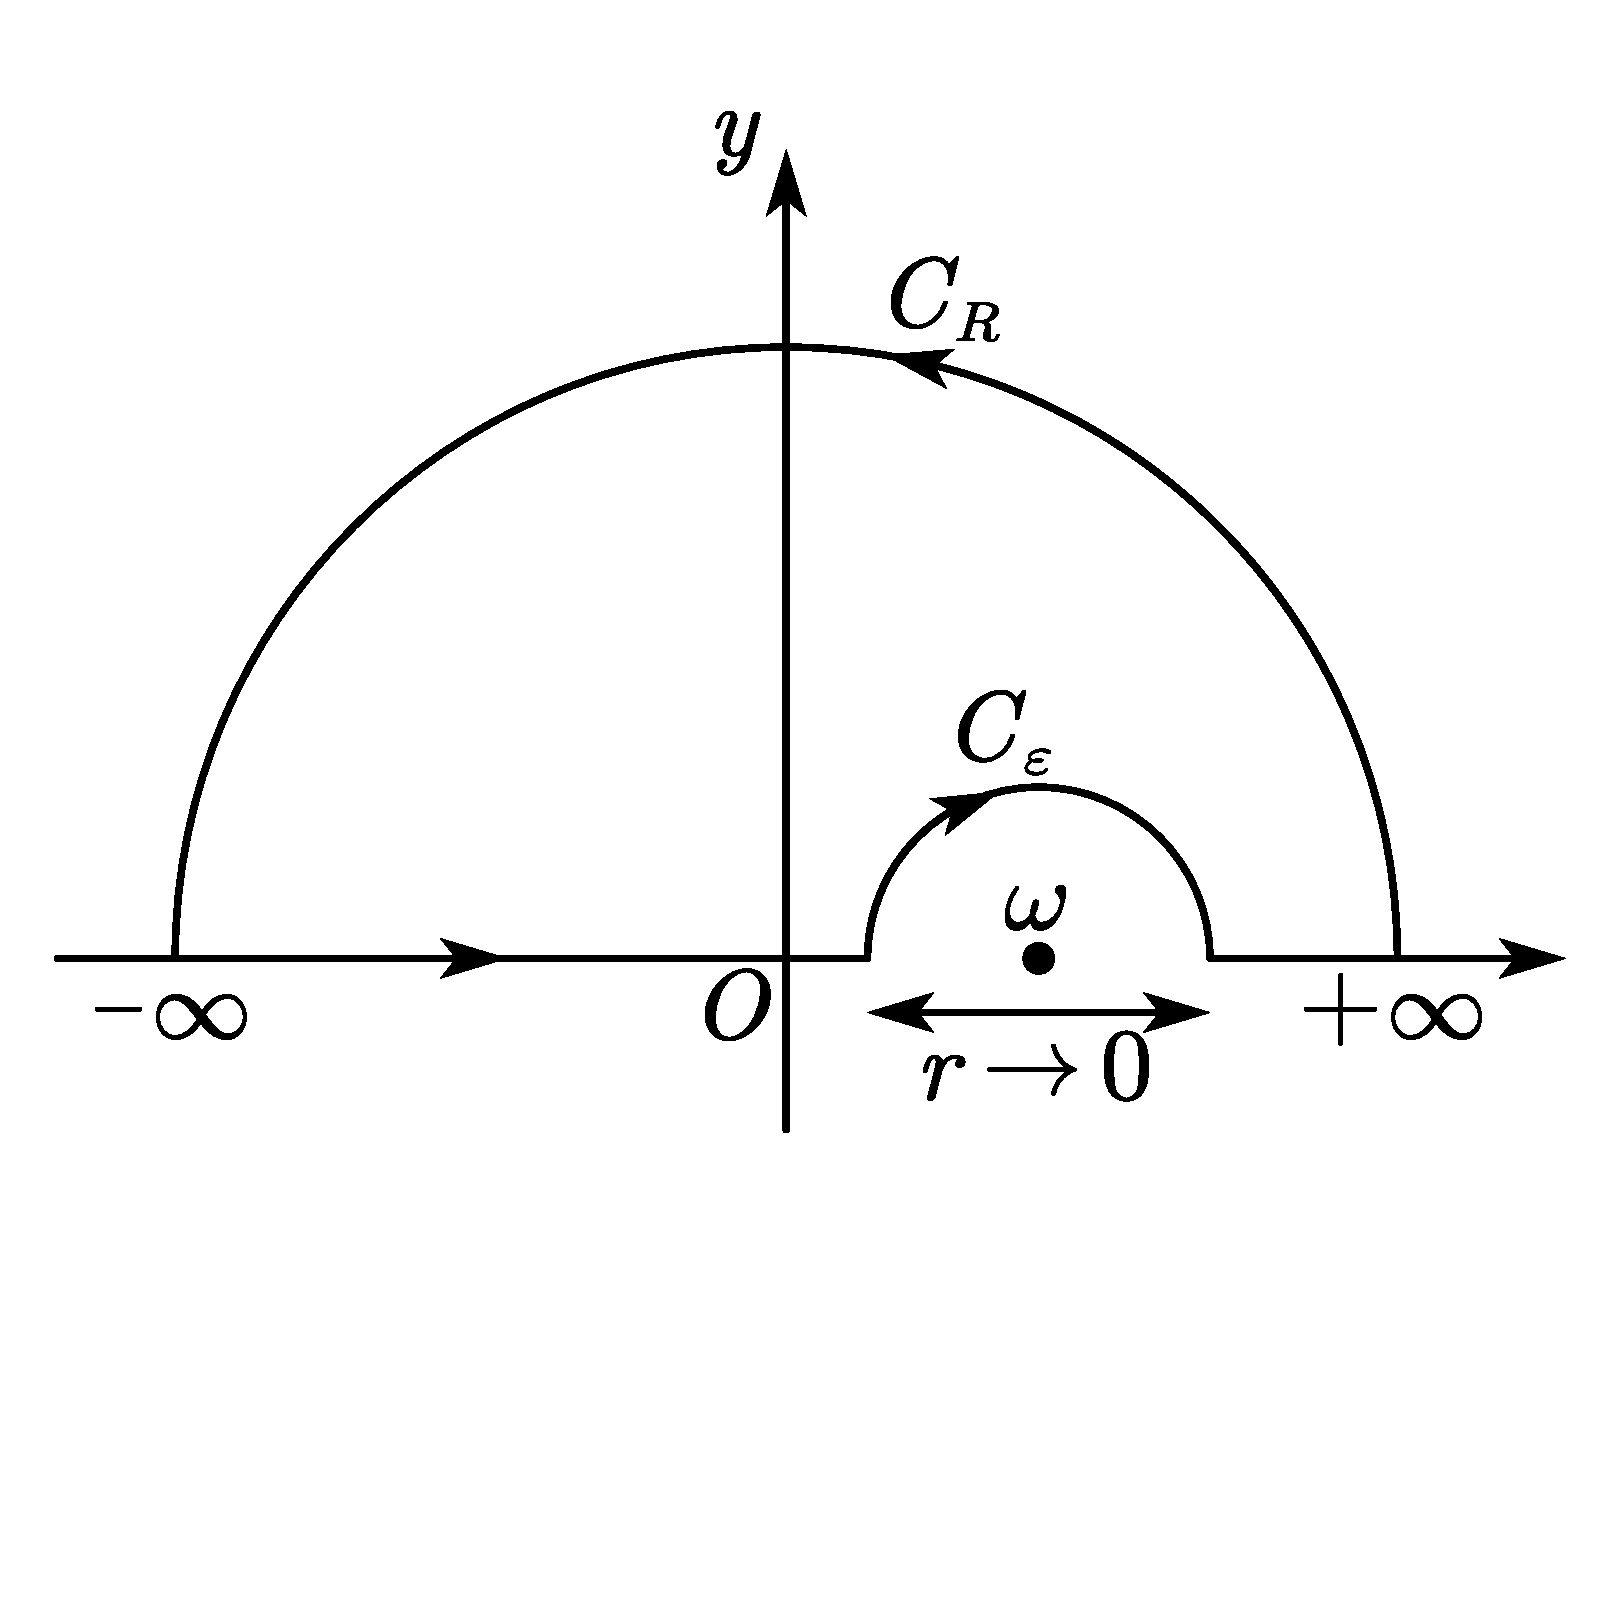
\includegraphics[width=7cm]{figure/k-k-relation.pdf}
        \caption{上半平面的围道积分}
        \end{figure}
     考虑如图的回路积分, 积分回路不包含实轴上的奇点, 所以如果函数是解析的, 积分应当等于零. 根据上面的分析, 推迟格林函数在上半复平面上解析, 且在无穷远处渐近地趋于零, 所以有
     \begin{equation}
         \oint \frac{G_{AB}^{\mathrm{R}}(z)}{z-\omega}\dd z=0,
     \end{equation}
回路积分可以分成三部分:
     \begin{equation}
        \left\{
            \begin{aligned}
                &\mbox{沿大圆积分}=0,\\
                &\mbox{沿实轴积分}=\mathcal{P}\int_{-\infty}^{\infty}\frac{G_{AB}^{\mathrm{R}}(\omega')}{\omega'-\omega}\dd\omega',\\
                &\mbox{沿小圆积分(由留数定理)}=-\mathrm{i}\pi G_{AB}^{\mathrm{R}}(\omega),
            \end{aligned}
        \right.
     \end{equation}
     于是得到
     \begin{equation}
         \mathcal{P}\int_{-\infty}^{\infty}\frac{G_{AB}^{\mathrm{R}}(\omega')}{\omega'-\omega}\dd\omega'-\mathrm{i}\pi G_{AB}^{\mathrm{R}}(\omega)=0.\label{k-k-relation1}
     \end{equation}
     如果把推迟格林函数拆分成实部和虚部两部分, 即
     \begin{equation}
         G_{AB}^{\mathrm{R}}(\omega)=\mathrm{Re}G_{AB}^{\mathrm{R}}(\omega)+\mathrm{i}\mathrm{Im}G_{AB}^{\mathrm{R}}(\omega),
     \end{equation}
    对比式中的实部和虚部, 就得到了推迟格林函数的 Kramers-Kronig 色散关系:
    \begin{equation}
        \boxed{\left\{ \begin{aligned}
                    \mathrm{Re}G_{AB}^{\mathrm{R}}(\omega)&=\frac{1}{\pi}\int_{-\infty}^\infty\frac{\mathrm{Im}G_{AB}^{\mathrm{R}}(\omega')}{\omega'-\omega}\dd \omega',\\
                    \mathrm{Im}G_{AB}^{\mathrm{R}}(\omega)&=-\frac{1}{\pi}\int_{-\infty}^{\infty}\frac{\mathrm{Re}G_{AB}^{\mathrm{R}}(\omega')}{\omega'-\omega}\dd \omega'.
        \end{aligned}\right.}
    \end{equation}
    \begin{question}{}{}
        推导超前格林函数 $G_{AB}^{\mathrm{A}}(\omega)$ 的 Kramers-Kronig 色散关系.
    \end{question}

\section{$G_{AB}^{\mathrm{R}}(\omega)$ 的若干应用}

    (1)  $G_{AB}^{\mathrm{R}}$ 本身即为某种关联函数或者传播子. 
    
    (2)  $\langle \hat{B}\hat{A} \rangle_T$ 用 $G_{AB}^{\mathrm{R,A}}(\omega)$ 表示 (谱定理).
    
    由谱函数表达式出发,
        \begin{align}
            A(\omega)&=\frac{1}{\mathcal{Z}}\sum_m\sum_n\mathrm{e}^{-\beta E_m}\left( \mathrm{e}^{-\beta(E_n-E_m)}+\epsilon \right) B_{mn}A_{nm}\delta(E_m-E_n-\omega)\nonumber\\
            &=\frac{1}{\mathcal{Z}}\sum_m\sum_n\mathrm{e}^{-\beta E_m}\left( \mathrm{e}^{\beta\omega}+\epsilon \right) B_{mn}A_{nm}\delta(E_m-E_n-\omega),
        \end{align}
    然后考虑下面的函数:
 \begin{align}\label{average1}
            \int_{-\infty}^{\infty}\frac{A(\omega')}{\mathrm{e}^{\beta\omega'}+\epsilon}\dd\omega'&=\int_{-\infty}^{\infty}\frac{1}{\mathcal{Z}}\sum_m\sum_n\mathrm{e}^{-\beta E_m}B_{mn}A_{nm}\delta(E_m-E_n-\omega')\dd\omega'\nonumber\\
            &=\frac{1}{\mathcal{Z}}\sum_m\sum_n\mathrm{e}^{-\beta E_m}B_{mn}A_{nm}\nonumber\\
            &=\sum_m\sum_n\left\langle m \left| \frac{\mathrm{e}^{-\beta E_m}}{\mathcal{Z}}\hat B \right| n \right\rangle \langle n|\hat A |m \rangle\nonumber\\
            &=\sum_m\left\langle m\left| \frac{\mathrm{e}^{-\beta E_m}}{\mathcal{Z}}\hat B\hat A \right|m \right\rangle\nonumber\\
            &=\mathrm{Tr}\left[ \frac{\mathrm{e}^{-\beta E_m}}{\mathcal{Z}}\hat B\hat A \right]\nonumber\\
            &=\left\langle \hat B\hat A \right\rangle_T,
        \end{align}
这样就得到了用谱函数计算任意两算符关联函数的表达式, 这一关系式也经常被称为\textbf{谱定理}, 即:
\begin{equation}\label{eq242}
\boxed{
\left\langle \hat B\hat A \right\rangle_T=\int_{-\infty}^{\infty}\frac{A(\omega')}{\mathrm{e}^{\beta\omega'}+\epsilon}\dd\omega'.
}
\end{equation}
将式 \eqref{spectrum2} 带入上式, 就得到了
    \begin{equation}
        \left\langle \hat{B}\hat{A} \right\rangle_T=-\frac{1}{2\pi\mathrm{i}}\int_{-\infty}^{\infty}\frac{G_{AB}^{\mathrm{R}}(\omega')-G_{BA}^{\mathrm{A}}(\omega')}{\mathrm{e}^{\beta\omega'}+\epsilon}\dd\omega'.
    \end{equation}

    (3)  $G_{AB}^{\mathrm{R}}(\omega)$ 与多体系统激发谱之间的关系.
    \begin{equation}
        \begin{aligned}
            G_{AB}^{\mathrm{R}}(\omega)&=\int_{-\infty}^{\infty}\frac{A(\omega')}{\omega-\omega'+\mathrm{i}\eta}\dd\omega'\\
            &=\int_{-\infty}^{\infty}\frac{\mathrm{d}\omega'}{\omega-\omega'+\mathrm{i}\eta}\cdot \frac{1}{\mathcal{Z}}\sum_n\sum_m\left( \mathrm{e}^{-\beta E_n}+\epsilon \mathrm{e}^{-\beta E_m} \right) B_{mn}A_{nm} \delta(E_m-E_n-\omega')\\
            &=\frac{1}{\mathcal{Z}}\sum_m\sum_n\frac{1}{\omega-(E_m-E_n)+\mathrm{i}\eta}\left( \mathrm{e}^{-\beta E_n}+\epsilon \mathrm{e}^{-\beta E_m} \right) B_{mn}A_{nm},
        \end{aligned}\label{excite1}
    \end{equation} 
    其中, 取零温极限 $T\to 0$, $\beta\to\infty$, 只保留最大项 $m=0$ 和 $n=0$, 配分函数可以表示成
\begin{align}
            \mathcal{Z}&=\mathrm{Tr}\left[ \mathrm{e}^{-\beta \hat{H}} \right]=\sum_m \langle m|\mathrm{e}^{-\beta\hat H}|m \rangle\nonumber\\
            &=\sum_m\mathrm{e}^{-\beta E_m}=\mathrm{e}^{-\beta E_0}+\mathrm{e}^{-\beta E_1}+\cdots\nonumber\\
            &\approx \mathrm{e}^{-\beta E_0},
        \end{align}
    于是式 \eqref{excite1} 中两项分别可以写成
    \begin{equation}
        \left\{
        \begin{aligned}
            \mbox{第一项}&=\frac{1}{\mathrm{e}^{-\beta E_0}}\sum_m\frac{\mathrm{e}^{-\beta E_0}}{\omega-(E_m-E_0)+\mathrm{i}\eta}B_{m0}A_{0m},\\
            \mbox{第二项}&=\frac{\epsilon}{\mathrm{e}^{-\beta E_0}}\sum_n\frac{\mathrm{e}^{-\beta E_0}}{\omega-(E_0-E_n)+\mathrm{i}\eta}B_{0n}A_{n0},
        \end{aligned}
        \right.
    \end{equation}
    于是格林函数可以表示成
    \begin{equation}
        G_{AB}^{\mathrm{R}}(\omega)=\sum_n\left[ \frac{B_{n0}A_{0n}}{\omega-(E_n-E_0)+\mathrm{i}\eta}+\frac{\epsilon B_{0n}A_{n0}}{\omega+(E_n-E_0)+\mathrm{i}\eta} \right],
    \end{equation}
    相应地有
    \begin{equation}
        G_{AB}^{\mathrm{R}}(t)=-\mathrm{i}\theta(t)\langle 0|[\hat{A}(t),\hat{B}]_\epsilon|0 \rangle.
    \end{equation}
    
选取合适的表象, 使得矩阵元非零并给出低能激发态, 那么 $G_{AB}^{\mathrm{R}}(z)$ 的极点正的实坐标确定多体系统的激发谱.
   
    (4)  $\hat{A}\hat{B}$ 是厄米算符的情况.
     
    考虑算符的系综平均应当是实值, 有
    \begin{equation}
        \left\langle \hat{B}\hat{A} \right\rangle_T=\int_{-\infty}^{\infty}\frac{A(\omega')}{\mathrm{e}^{\beta \omega'}+\epsilon}\dd\omega',
    \end{equation} 
    等式右边 $A(\omega')$ 应当也是实量, 或者虚部积分为零, 即
    \begin{equation}
        \int_{-\infty}^{\infty}\frac{\mathrm{Im}A(\omega')}{\mathrm{e}^{\beta\omega'}+\epsilon}\dd \omega'=0.
    \end{equation}
    下面我们考虑 $A(\omega')$ 为实量的情况. 根据推迟和超前格林函数的谱表示,
    \begin{equation}
        G_{AB}^{\mathrm{R}}(\omega)=\int_{-\infty}^{\infty}\frac{A(\omega')}{\omega-\omega'+\mathrm{i}\eta}\dd\omega',\quad G_{AB}^{\mathrm{A}}(\omega)=\int_{-\infty}^{\infty}\frac{A(\omega')}{\omega-\omega'-\mathrm{i}\eta}\dd\omega',
    \end{equation}
    可以得到
    \begin{equation}
        \left[ G_{AB}^{\mathrm{R}}(\omega) \right]^*=G_{AB}^{\mathrm{A}}(\omega),
    \end{equation}
    所以两格林函数的实部和虚部之间的关系是
    \begin{equation}
        \left\{
            \begin{aligned}
                \mathrm{Re}G_{AB}^{\mathrm{R}}(\omega)&=\mathrm{Re}G_{AB}^{\mathrm{A}}(\omega),\\
                \mathrm{Im}G_{AB}^{\mathrm{R}}(\omega)&=-\mathrm{Im}G_{AB}^{\mathrm{A}}(\omega),
            \end{aligned}
        \right.
    \end{equation}
    带入谱定理式 \eqref{spectrum2}, 得到
   \begin{align}
            A(\omega)&=-\frac{1}{2\pi \mathrm{i}}\left[ G_{AB}^{\mathrm{R}}(\omega)-G_{AB}^{\mathrm{A}}(\omega) \right]\nonumber\\
            &=-\frac{1}{2\pi\mathrm{i}}\left[ G_{AB}^{\mathrm{R}}(\omega)-\left( G_{AB}^{\mathrm{R}}(\omega) \right)^* \right]\nonumber\\
            &=-\frac{1}{2\pi\mathrm{i}}\left[ \mathrm{i} 2\mathrm{Im}G_{AB}^{\mathrm{R}}(\omega) \right]\nonumber\\
            &=-\frac{1}{\pi}\mathrm{Im}G_{AB}^{\mathrm{R}}(\omega),
        \end{align}
    代回 \eqref{spectrum1} 及 \eqref{eq242}, 就得到两个十分重要的表达式
    \begin{equation}
        \boxed{G_{AB}^{\mathrm{R,A}}(\omega)=\int_{-\infty}^{\infty}\left( \mp\frac{1}{\pi} \right) \frac{\mathrm{Im} G_{AB}^{\mathrm{R,A}}(\omega')\dd \omega'}{\omega-\omega'\pm \mathrm{i}\eta},}
    \end{equation}
    以及
    \begin{equation}
        \boxed{\left\langle \hat{B}\hat{A} \right\rangle_T=\int_{-\infty}^{\infty}-\frac{1}{\pi}\frac{\mathrm{Im}G_{AB}^{\mathrm{R}}(\omega')}{\mathrm{e}^{\beta\omega'}+\epsilon}\dd\omega'.}
    \end{equation}
    \begin{note}
        特别地, 下面简单讨论一下当 $\hat{F}=\hat{B}\hat{A}$ 是厄米算符时, 在什么情况下谱函数 $A(\omega)$ 会是实数. 我们考虑以下两种情况:
        
        (i) $\hat{A}$ 和 $\hat{B}$ 都不是厄米算符, 但 $\hat{B}\hat{A}$ 是厄米算符.

        在这种情况下, 算符具有性质
        \begin{equation}
            \left( \hat{B}\hat{A} \right)^\dagger =\hat{A}^\dagger \hat{B}^\dagger =\hat{B}\hat{A},
        \end{equation}
        具有这种性质的算符对的例子有 $\hat{A}=\hat{C}_{k\sigma}$ 和 $\hat{B}=\hat{C}_{k\sigma}^\dagger$ 等. 谱函数可以表示成
        \begin{equation}
            A(\omega)=\frac{1}{\mathcal{Z}}\sum_n\sum_m\left( \mathrm{e}^{-\beta E_n}+\epsilon \mathrm{e}^{-\beta E_m} \right) B_{mn}A_{nm}\delta\left( E_m-E_n-\omega \right),
        \end{equation}
        谱函数的厄米共轭:
        \begin{equation}
            A^*(\omega)=\frac{1}{\mathcal{Z}}\sum_n\sum_m\left( \mathrm{e}^{-\beta E_n}+\epsilon \mathrm{e}^{-\beta E_m} \right) (B_{mn})^* (A_{nm})^*\delta\left( E_m-E_n-\omega \right),
        \end{equation}
        其中算符矩阵元的乘积具体表示为
        \begin{equation}
            B_{mn}A_{nm}=\langle m|\hat{B}|n \rangle\langle n|\hat{A}|m \rangle,
        \end{equation}
        以及
     \begin{align}
                (B_{mn})^* (A_{nm})^*=&\langle m|\hat{B}|n \rangle^*\langle n|\hat{A}|m \rangle^*\nonumber\\
                =&\langle n|\hat{B}^\dagger |m \rangle \langle m|\hat{A}^\dagger |n \rangle\nonumber\\
                =&\langle n|\hat{A}|m \rangle\langle m|\hat{B}|n \rangle\nonumber\\
                =&B_{mn}A_{nm}.
     \end{align}
        因此在这种情况下, 谱函数满足
        \begin{equation}
            A^*(\omega)=A(\omega)
        \end{equation}
        是实数.

        (ii) 如果算符 $\hat{A}$ 和 $\hat{B}$ 都是厄米算符, 且 $\left[ \hat{A},\hat{B} \right]=0$, 从而 $\hat{F}=\hat{B}\hat{A}$ 是厄米算符.

        此时考虑算符矩阵元的乘积, 有
        \begin{equation}
            (B_{mn})^* (A_{nm})^*=\langle n|\hat{B}|m \rangle \langle m|\hat{A}|n \rangle\ne B_{mn}A_{nm},
        \end{equation}
        因此这种情况下不满足 $\hat{A}(\omega)=\hat{A}^*(\omega)$, 谱函数不是实数.

        综上讨论, 只有当算符 $\hat{A}$ 和 $\hat{B}$ 都不是厄米算符, 但 $\hat{B}\hat{A}$ 是厄米算符时, 谱函数是实数.
    \end{note}

\section{运动方程法}
以全同自由费米子系统为例, 设系统的粒子数为 $N$, 哈密顿量是
\begin{equation}
    \hat{H}=\sum_{k\sigma}E^{}_k\hat{C}_{k\sigma}^\dagger \hat{C}_{k\sigma}^{ },
\end{equation}
下面讨论如何求解这一系统的格林函数具体形式. 

格林函数的表达式是
\begin{equation}
    G_{AB}^{\mathrm{R}}(t)=-\mathrm{i}\theta(t)\left\langle \left[ \hat{C}_{k\sigma}^{ }(t),\hat{C}_{k\sigma}^{\dagger} \right]_+ \right\rangle_T,
\end{equation}
上式对时间求导数, 有
  \begin{align}\label{motion-eq1}
        \mathrm{i}\frac{\dd}{\dd t}G^{\mathrm{R}}(t)&=\mathrm{i}\frac{\dd}{\dd t}\left\{ -\mathrm{i}\theta(t)\left\langle \left[ \hat{C}_{k\sigma}^{ }(t),\hat{C}_{k\sigma}^{\dagger} \right]_+ \right\rangle_T \right\}\nonumber\\
        &=\left( \frac{\dd}{\dd t}\theta(t) \right) \left\langle \left[ \hat{C}_{k\sigma}^{ }(t),\hat{C}_{k\sigma}^{\dagger} \right]_+ \right\rangle_T-\mathrm{i}\theta(t)\left\langle \left[ \mathrm{i}\frac{\dd}{\dd t}\hat{C}_{k\sigma}^{ }(t),\hat{C}_{k\sigma}^{\dagger} \right]_+ \right\rangle_T,
    \end{align}
其中, 阶跃函数 $\theta(t)$ 的傅里叶变换是
\begin{equation}
    \theta(t)=-\frac{1}{2\pi \mathrm{i}}\int_{-\infty}^{\infty}\frac{\mathrm{e}^{-\mathrm{i} xt}}{x+\mathrm{i}\eta}\dd x,
\end{equation}
对时间的导数就是
   \begin{align}\label{theta-fourier}
        \frac{\dd}{\dd t}\theta(t)&=-\frac{1}{2\pi\mathrm{i}}\int_{-\infty}^{\infty}\frac{(-\mathrm{i} x)\mathrm{e}^{-\mathrm{i} xt}}{x+\mathrm{i}\eta}\dd x\nonumber\\
        &=\frac{1}{2\pi}\int_{-\infty}^{\infty}\frac{x\mathrm{e}^{-\mathrm{i} xt}}{x+\mathrm{i}\eta}\dd x\nonumber\\
        &=\frac{1}{2\pi}\int_{-\infty}^{\infty}\frac{(x+\mathrm{i}\eta-\mathrm{i}\eta)\mathrm{e}^{-\mathrm{i} xt}}{x+\mathrm{i} \eta}\dd x\nonumber\\
        &=\frac{1}{2\pi}\int_{-\infty}^{\infty}\mathrm{e}^{-\mathrm{i} xt}\dd x-\frac{\mathrm{i}\eta}{2\pi}\int_{-\infty}^{\infty}\frac{\mathrm{e}^{-\mathrm{i} xt}}{x+\mathrm{i}\eta}\dd x\nonumber\\
        &=\delta(t)-\eta\theta(t),
    \end{align}
此外,式 \eqref{motion-eq1} 中第二项可以利用海森伯方程写成
  \begin{align}\label{heisenberg1}
        \mathrm{i}\frac{\dd}{\dd t}\hat{C}_{k\sigma}^{ }(t)&=\left[ \hat{C}_{k\sigma}(t),\hat{H} \right]_-\nonumber\\
        &=\left[ \mathrm{e}^{\mathrm{i}\hat{H}t}\hat{C}_{k\sigma}^{ }\mathrm{e}^{-\mathrm{i}\hat{H}t},\hat{H} \right]_-\nonumber\\
        &=\mathrm{e}^{\mathrm{i}\hat{H}t}\left[ \hat{C}_{k\sigma},\hat{H} \right]_-\mathrm{e}^{-\mathrm{i}\hat{H}t},
    \end{align}
其中, 考虑到在费米子系统中, 利用反对易式 $[\; ,\;]_+$ 计算更方便, 可以利用恒等式
\begin{equation}
    \left[ \hat{A},\hat{B}\hat{C} \right]_-=\left[ \hat{A},\hat{B} \right]_+\hat{C}-\hat{B}\left[ \hat{A},\hat{C} \right]_+,
\end{equation}
将对易式简化成
   \begin{align}
        \left[ \hat{C}_{k\sigma}^{ },\hat{H} \right]_- &=\left[ \hat{C}_{k\sigma},\sum_{k^\prime}\sum_{\sigma'}E_{k'}\hat{C}_{k^\prime\sigma'}^{\dagger} \hat{C}_{k^\prime\sigma'}^{ } \right]_-\nonumber\\
        &=\sum_{k^\prime}\sum_{\sigma'}E_{k'}\left[ \hat{C}_{k\sigma}^{ },\hat{C}_{k^\prime\sigma'}^{\dagger}\hat{C}_{k'\sigma'}^{ } \right]_-\nonumber\\
        &=\sum_{k'}\sum_{\sigma'}E_{k'}\left( \underbrace{\left[ \hat{C}_{k\sigma}^{ },\hat{C}_{k'\sigma'}^{\dagger} \right]_+}_{=\delta_{kk'}\delta_{\sigma\sigma'}} \hat{C}_{k'\sigma'}^{ }-\hat{C}_{k'\sigma'}^{\dagger}\underbrace{\left[ \hat{C}_{k\sigma}^{ },\hat{C}_{k'\sigma'}^{ } \right]_+}_{=0} \right)\nonumber\\
        &=\sum_{k'}\sum_{\sigma'}E_{k'}\delta_{kk'}\delta_{\sigma\sigma'}\hat{C}_{k'\sigma'}^{ }\nonumber\\
        &=E^{}_{k}\hat{C}_{k\sigma}^{ }.
    \end{align}
代回海森伯方程 \eqref{heisenberg1}, 得到
\begin{equation}
    \mathrm{i}\frac{\dd}{\dd t}\hat{C}_{k\sigma}(t)=E_k\hat{C}_{k\sigma}(t),\label{heisenberg2}
\end{equation}
将 \eqref{theta-fourier} 的结果和式 \eqref{heisenberg1} 带入格林函数对时间的导数 \eqref{motion-eq1}, 有
  \begin{align}
        \mathrm{i}\frac{\dd}{\dd t}G^{\mathrm{R}}(t)&=\left( \delta(t)-\eta\theta(t) \right)\left\langle \left[ \hat{C}_{k\sigma}^{ }(t),\hat{C}_{k\sigma}^{\dagger} \right]_+ \right\rangle_T-\mathrm{i}\theta(t)\left\langle \left[ E_k\hat{C}_{k\sigma}^{ }(t),\hat{C}_{k\sigma}^{\dagger} \right]_+ \right\rangle_T\nonumber\\
        &=\delta(t)\underbrace{\left\langle \left[ \hat{C}_{k\sigma}^{ },\hat{C}_{k\sigma}^{\dagger} \right]_+ \right\rangle_T}_{=1}-\mathrm{i}\eta G^{\mathrm{R}}(t)+E_kG^{\mathrm{R}}(t)\nonumber\\
        &=\delta(t)-\mathrm{i}\eta G^{\mathrm{R}}(t)+E_kG^{\mathrm{R}}(t),
    \end{align}
这样就得到了自由费米子系统的格林函数运动方程, 即
\begin{equation}
    \mathrm{i}\frac{\dd}{\dd t}G^{\mathrm{R}}(t)=\delta(t)-\mathrm{i}\eta G^{\mathrm{R}}(t)+E_kG^{\mathrm{R}}(t).\label{motion-eq2}
\end{equation}

如果考虑傅里叶变换
\begin{equation}
    \left\{\begin{aligned}
        G^{\mathrm{R}}(t)&=\frac{1}{2\pi}\int_{-\infty}^{\infty}G^{\mathrm{R}}(\omega)\mathrm{e}^{-\mathrm{i}\omega t}\dd \omega,\\
        \delta(t)&=\frac{1}{2\pi}\int_{-\infty}^{\infty}\mathrm{e}^{-\mathrm{i}\omega t}\dd \omega,
    \end{aligned}\right.
\end{equation}
带入式 \eqref{motion-eq2}, 就得到了
 \begin{align}
        \omega G^{\mathrm{R}}(\omega)&=-\mathrm{i}\eta G^{\mathrm{R}}(\omega)+E_k G^{\mathrm{R}}(\omega)+1\nonumber\\
        \Rightarrow G^{\mathrm{R}}(\omega)&=\frac{1}{\omega-E_k+\mathrm{i}\eta},
    \end{align}
于是谱函数可以表示成
\begin{equation}
    A(\omega)=-\frac{1}{\pi}\mathrm{Im}G^{\mathrm{R}}(\omega)=\delta(\omega-E_k).
\end{equation}

另外, 根据式 \eqref{average1}, 系统的粒子数密度平均值可以表示成
\begin{equation}
    \langle \hat{n}_{k\sigma} \rangle_T=\int\frac{\delta(\omega'-E_k)}{\mathrm{e}^{\beta\omega'}+1}\dd\omega'=\frac{1}{\mathrm{e}^{\beta E_k}+1},
\end{equation}
此即费米分布函数. 
\begin{question}{}{}
自由费米子系统中, 利用对易子 $[\; ,\;]_{-}$ 重新计算格林函数运动方程.
\end{question}

需要注意的是:
\begin{itemize}
\item 求系统的激发谱, 总粒子数不变, 选择的算符 $\hat A$ 和 $\hat B$ 也必须保持粒子数不变.
\item 对于有限温度下全同费米子系统或全同玻色子系统的一些量子统计, 考虑巨正则系综非常方便. 正则系综也能算出来, 但更复杂.
\end{itemize}

下面计算粒子态密度. 考虑巨正则系综, 总粒子数可以表示为:
\begin{align}
N= &\langle\hat{N}\rangle_{\mu}=\left\langle\sum_{k  \sigma} \hat{n}_{k  \sigma}\right\rangle_{\mu}=\sum_{k  \sigma}\left\langle\hat{n}_{k  \sigma}\right\rangle_{\mu} \nonumber\\
=&\sum_{k  \sigma} \int_{-\infty}^{\infty} \frac{-\frac{1}{\pi} \operatorname{Im} G^{\mathrm{R}}_{k }(\omega)}{\mathrm{e}^{\beta \omega}+1} \mathrm{d} \omega\nonumber \\
\xlongequal[]{\omega \rightarrow \omega-\mu}& \sum_{k  \sigma} \int_{-\infty}^{\infty} \frac{-\frac{1}{\pi} \operatorname{Im} G^{\mathrm{R}}_{k }(\omega-\mu)}{\mathrm{e}^{\beta(\omega-\mu)}+1} \mathrm{~d} \omega\nonumber \\
\equiv&\int_{-\infty}^{\infty} n_{\mathrm{F}}(\omega) \rho(\omega) \mathrm{d} \omega ,
\end{align}
其中 $\displaystyle n_{\mathrm{F}}(\omega)=\frac{1}{\mathrm{e}^{\beta (\omega-\mu)}+1}$ 是费米子分布概率(平均占据数). $\rho(\omega)$ 就是粒子态密度, 也称为态密度, 具体表达式为:
\begin{equation}
\rho(\omega) =\sum_{k  \sigma}\left[-\frac{1}{\pi} \operatorname{Im} G^{\mathrm{R}}_{k }(\omega-\mu)\right] .
\end{equation}
虽然这个结果是用无相互作用系统推出的, 但其是普适的. 对于有相互作用系统, 只需要将 $G^{\mathrm{R}}_{k }$ 替换为有相互作用的格林函数即可.

回到无相互作用系统, 在三维情况下 
\begin{equation}
\rho(\omega) =\sum_{k  \sigma} \delta\left(\omega-E_{k}^0 \right)\propto \sqrt{\omega}.
\end{equation}

\begin{question}{}{}
已知相互作用系统的哈密顿量
\begin{equation}
\hat{H}=\sum_{k  \sigma} (E_{k}^{(1)}-\mu) \hat{a}_{k  \sigma}^{\dagger} \hat{a}_{k  \sigma}^{}+\sum_{k  \sigma} (E_{k}^{(2)}-\mu) \hat{b}_{k  \sigma}^{\dagger} \hat{b}_{k  \sigma}^{}+V\sum_{k  \sigma} \left(\hat{a}_{k  \sigma}^{\dagger} \hat{b}_{k  \sigma}^{}+\hat{b}_{k  \sigma}^{\dagger} \hat{a}_{k  \sigma}^{}\right),
\end{equation}
分别计算 $a$ 带和 $b$ 带的粒子态密度.
\end{question}

\section{格林函数方法的实际应用}
\subsection{对铁磁海森伯模型的应用}
在固体中, 处于格点上的原子核和电子都带有自旋, 因此每个格点上会呈现出磁矩. 磁矩不为零的格点称为磁性格点. 多数情况下, 不同磁性格点上磁矩的取向不同. 当有外磁场时, 磁矩倾向于平行外磁场排列. 但某些铁磁体物质(如铁, 钴, 镍等)在温度不太高时, 即使无外磁场, 每个磁性格点上磁矩也会平行排列, 在宏观上表现出磁化强度, 这种情况称为自发磁化. 有的物质在自发磁化时, 相邻磁性格点上的磁矩取向相反, 这种物质称为反铁磁体.
如果相邻磁性格点的磁矩取向相反, 但大小不等, 则称为亚铁磁体. 

铁磁性是一种量子力学效应, 由于电子的全同性, 两个电子体系的波函数必须反对称. 如果两电子自旋同向(自旋波函数对称), 则其轨道波函数反对称; 如果自旋反向, 轨道波函数应该对称. 由波函数的对称性, 造成两个电子间库仑作用的一种特殊贡献, 称为交换能, 以下记作 $J$. 这一物理量与两电子的自旋状态有关. 下面具体讨论铁磁海森伯模型的应用.
\subsubsection{海森伯模型}
海森伯模型是描述量子磁性的基本模型, 这一模型同时可以很好地描述一些由量子自旋算符带来的效应. 通过研究海森伯模型的基态, 激发态和热力学相, 人们得到了很多重要的物理概念和技术. 该模型由海森伯于1928年提出, 后来Dirac于1929年给出自旋为 $1 / 2$ 时该模型哈密顿量的证明, 1963年Anderson证明了自旋大于 $1 / 2$ 时的海森伯模型. 


海森伯模型的哈密顿量为:
\begin{equation}
\hat{H}=-{\sum_{ll^{\prime}}}^{\prime} J_{l l^{\prime}} \hat{\boldsymbol{S}}_{l} \cdot \hat{\boldsymbol{S}}_{l^{\prime}},
\end{equation}
其中 $\displaystyle{\sum_{ll^{\prime}}}^{\prime}$ 表示对 $l\neq l'$ 的全部格点求和, $\hat{\boldsymbol{S}}_{l}$ 表示第 $l$ 个格点的自旋算符. $J_{l l^{\prime}}$ 从泡利不相容原理来, 是交换积分. 当$J_{l l^{\prime}}>0$ 时可以描述铁磁体, $J_{l l^{\prime}}<0$ 时可以描述反铁磁体. 下面给出几个常见的“海森伯”模型.

设哈密顿量为:
\begin{equation}
\hat{H}=-{\sum_{ll^{\prime}}}^{\prime} J_{l l^{\prime}}\left[\alpha\left(\hat{S}_{l}^{x} \hat{S}_{l^{\prime}}^{x}+\hat{S}_{l}^{y} \hat{S}_{l^{\prime}}^{y}\right)+\beta \hat{S}_{l}^{z} \hat{S}_{l^{\prime}}^{z}\right],
\end{equation}
其中 $\alpha\left(\hat{S}_{l}^{x} \hat{S}_{l^{\prime}}^{x}+\hat{S}_{l}^{y} \hat{S}_{l^{\prime}}^{y}\right)$ 是横向部分, $\beta \hat{S}_{l}^{z} \hat{S}_{l^{\prime}}^{z}$ 是纵向部分, 两部分在自旋动力学中作用不同. 有如下几种情况: 
\begin{itemize}
\item $\alpha=\beta=1$, 海森伯模型——无严格解; 
\item $\alpha=1, \beta=0$,  X-Y 模型——部分(低维)有严格解;
\item $\alpha=0, \beta=1$, Ising 模型——部分(低维)有严格解.
\end{itemize}
对于海森伯模型, 如果
\begin{equation}
\alpha=\beta=1, J_{l l^{\prime}}=J \delta_{l^{\prime}, l+\rho},
\end{equation}
其中 $\rho$ 表示最近邻格点的矢差, 这时的模型称为各向同性紧束缚海森伯模型. 下面我们主要讨论该模型, 其哈密顿量为:
\begin{equation}
\hat{H}=-J \sum_{l} \sum_{\rho} \hat{\boldsymbol{S}}_{l} \cdot \hat{\boldsymbol{S}}_{l+\rho}.
\end{equation}

在进一步讨论这个模型前, 我们先回顾一下有关自旋算符的内容:
\begin{itemize}
\item 自旋算符间的对易关系
\begin{equation}
\left[\hat{S}_{l}^{\alpha}, \hat{S}_{l^{\prime}}^{\beta}\right]_{-}=\mathrm{i} \varepsilon_{\alpha \beta \gamma} \hat{S}_{l}^{\gamma} \delta_{l l^{\prime}}, \quad \alpha, \beta, \gamma=x, y, z.
\end{equation}

\item 升降算符
\begin{equation}
\hat{S}_{l}^{\pm}=\hat{S}_{l}^{x} \pm \mathrm{i} \hat{S}_{l}^{y},
\end{equation}
满足对易式
\begin{equation}\label{sjsfdy}
\left[\hat{S}_{l}^{\pm}, \hat{S}_{l^{\prime}}^{z}\right]_{-}=\mp \hat{S}_{l}^{\pm} \delta_{l l^{\prime}}, \quad\left[\hat{S}_{l}^{+}, \hat{S}_{l^{\prime}}^{-}\right]_{-}=2 \hat{S}_{l}^{z} \delta_{l l^{\prime}}.
\end{equation}

\item $\hat{S}_{l}^{2}$ 和 $\hat{S}_{l}^{z}$的共同本征态 $|S, m\rangle_{l}$
\begin{align}
\hat{S}_{l}^{2}|S, m\rangle_{l}&=S(S+1)|S, m\rangle_{l} , \nonumber\\
\hat{S}_{l}^{z}|S, m\rangle_{l}&=m|S, m\rangle_{l} , \nonumber\\
\hat{S}_{l}^{+}|S, m\rangle_{l}&=\sqrt{(S-m)(S+m+1)}|S, m+1\rangle_{l} ,\nonumber \\
\hat{S}_{l}^{-}|S, m\rangle_{l}&=\sqrt{(S+m)(S-m+1)}|S, m-1\rangle_{l} .
\end{align}
其中 $m=-S,-S+1,\cdots,S$, 且有
\begin{equation}
\hat{S}_{l}^{+}|S, m=S\rangle_{l}=0, \quad \hat{S}_{l}^{-}|S,m=-S\rangle_{l}=0.
\end{equation}
对于含有 $N$ 个格点的体系, 体系自旋空间的维数(本征态的个数)将是 $(2 S+1)^{N}$.
\end{itemize}

\subsubsection{铁磁海森伯模型的若干理论结果}
考虑各向同性的铁磁海森伯模型, 其哈密顿量为:
\begin{align}
\hat{H} &=-J \sum_{l} \sum_{\rho} \hat{\boldsymbol{S}}_l \cdot \hat{\boldsymbol{S}}_{l+\rho}\nonumber \\
&=-J \sum_{l} \sum_{\rho}\left[\hat{S}_{l}^{z} \hat{S}_{l+\rho}^{z}+\frac{1}{2}\left(\hat{S}_{l}^{+} \hat{S}_{l+\rho}^{-}+\hat{S}_{l}^{-} \hat{S}_{l+\rho}^{+}\right)\right] \nonumber\\
&=-J \sum_{l} \sum_{\rho}\left(\hat{S}_{l}^{z} \hat{S}_{l+\rho}^{z}+\hat{S}_{l}^{-} \hat{S}_{l+\rho}^{+}\right) .
\end{align}
对于铁磁海森伯模型, $J>0$. 上式最后一行利用了不同格点间算符的对易关系\eqref{sjsfdy}, 同时考虑到求和是对全体格点进行的. 下面简单讨论一下铁磁海森伯模型的基态和激发态.

(a) 基态、激发态

1. 基态

直接考虑能量的基态并不容易, 通常我们寻找与哈密顿量对易的算符, 求得共同本征态, 进而确定能量本征态. 这里我们可以考虑总自旋算符和沿 $z$ 方向的总自旋算符:
\begin{equation}
\hat{\boldsymbol{S}}_{\mathrm{tot}}=\sum_{l} \hat{\boldsymbol{S}}_{l}, \quad \hat{S}_{\mathrm{tot}}^{z}=\sum_{l} \hat{S}_{l}^{z} .
\end{equation}
注意到:
\begin{align} 
{\left[\sum_{l, \rho} \hat{S}_{l}^{-} \hat{S}_{l+\rho}^{+}, \sum_{l^{\prime}} \hat{S}_{l^{\prime}}^{z}\right]_{-} } 
&=\sum_{l, \rho} \sum_{l^{\prime}}\left[\hat{S}_{l}^{-} \hat{S}_{l+\rho}^{+}, \hat{S}_{l^{\prime}}^{z}\right]_{-} \nonumber\\ 
&=\sum_{l, \rho} \sum_{l^{\prime}}\left(\hat{S}_{l}^{-}\left[\hat{S}_{l+\rho}^{+}, \hat{S}_{l^{\prime}}^{z}\right]_{-}+\left[\hat{S}_{l}^{-}, \hat{S}_{l^{\prime}}^{z} \right]_{-}\hat{S}_{l+\rho}^{+}\right)\nonumber\\ 
&=\sum_{l, \rho} \sum_{l^{\prime}}\left(-\hat{S}_{l}^{-} \hat{S}_{l^{\prime}}^{+} \delta_{l+\rho,l^{\prime}}+\hat{S}_{l^{\prime}}^{-} \hat{S}_{l+\rho}^{+} \delta_{l l^{\prime}}\right)\nonumber \\ 
&=0 ,
\end{align}
可以得到: 
\begin{equation}
\left[\hat{H}, \hat{S}_{\text {tot }}^{z}\right]_{-}=0. 
\end{equation}
所以 $\hat{H}$ 和 $\hat{S}_{\text {tot }}^{z}$ 有共同本征态, 利用前面给出的 $\hat{S}_{l}^{2}$ 和 $\hat{S}_{l}^{z}$ 的共同本征态, 可以得到体系的本征态为: $\displaystyle\prod_{l}|S, m\rangle_{l}$, 可以预期体系的基态是自旋全部同向排列, 即 $\displaystyle\prod_{l}|S, S\rangle_{l}$:
\begin{equation}
\hat{S}_{\text{tot}}^{z} \prod_{l}|S, S\rangle_{l}=N S \prod_{l}|S, S\rangle_{l}.
\end{equation}
\begin{figure}[htbp]
    \centering
    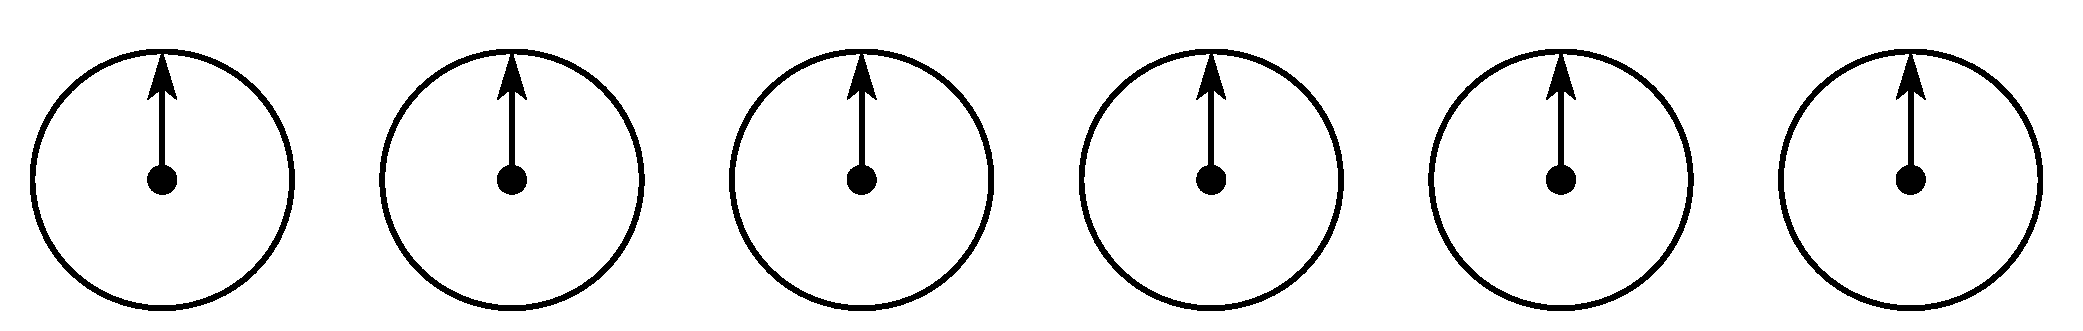
\includegraphics[width=10cm]{figure/ground-state.pdf}
    \caption{铁磁海森伯模型的基态.}
\end{figure}
\\将 $\displaystyle\prod_{l}|S, S\rangle_{l}$ 记为 $|g\rangle$, 可以证明 $|g\rangle$ 也是哈密顿算符 $\hat{H}$ 的本征态, 对应的本征值为 $E_g$:
\begin{equation}\label{HW7}
\hat{H}|g\rangle=E_{g}|g\rangle=-J S^{2} N Z |g\rangle,
\end{equation}
其中 $Z$ 为配位数.
\begin{question}{}{}
证明式\eqref{HW7}.
\end{question}

2. 自旋缺陷态

考虑某一个格点上的自旋偏转, 此时相当于基态模型在某一个格矢 $\boldsymbol{l}$ 所标记的格点上产生了一个自旋缺陷.
\begin{figure}[htbp]
    \centering
    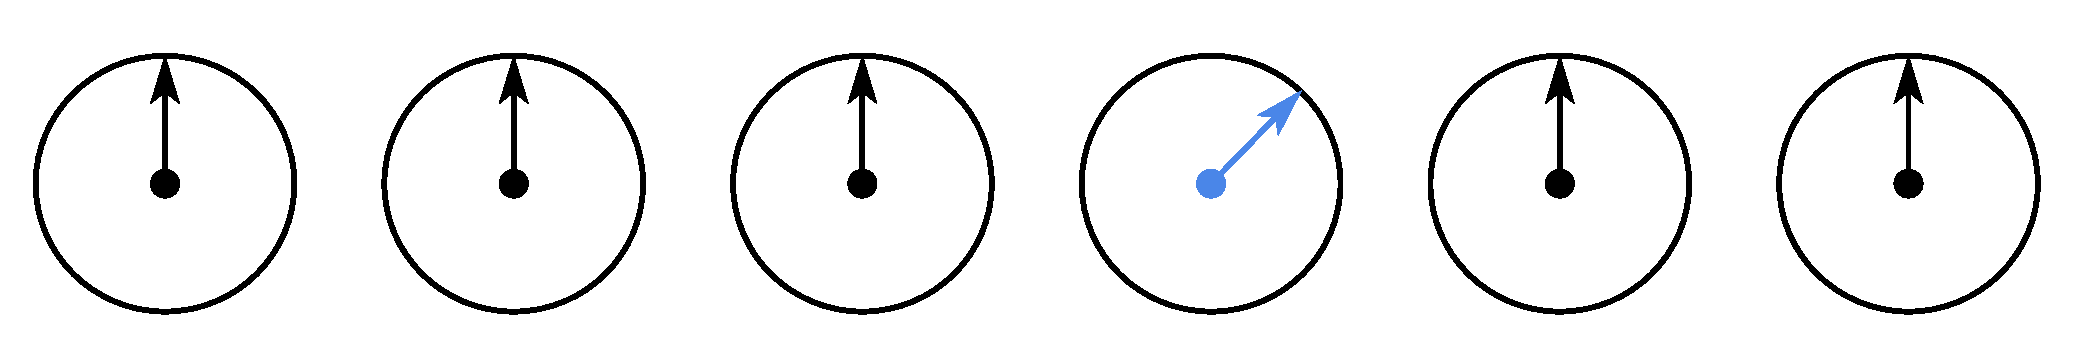
\includegraphics[width=10cm]{figure/excite-state.pdf}
    \caption{铁磁海森伯模型的自旋缺陷态.}
\end{figure}
\\ 记这一自旋缺陷态为 $|\boldsymbol{l}\rangle$, 满足
\begin{equation}
|\boldsymbol{l}\rangle \propto \hat{S}_{l}^{-}|g\rangle.
\end{equation}
可以证明, 归一化后的自旋缺陷态是
\begin{equation}
|\boldsymbol{l}\rangle = \frac{1}{\sqrt{2S}}\hat{S}_{l}^{-}|g\rangle.
\end{equation}
\begin{proof}
    设自旋缺陷态为
    \begin{equation}
        |\boldsymbol{l}\rangle=C\hat{S}_l^-|g\rangle,
    \end{equation}
    其中 $C$ 是待定常系数. 由归一化条件 $\langle l|l \rangle=\mathbbm{1}$, 得到
    \begin{equation}
        \begin{aligned}
            \left\langle g \left|\left( \hat{S}_l^- \right)^\dagger \hat{S}_l^- \right| g \right\rangle |C|^2=&\left(\sqrt{2S}\right)^2 |C|^2\\
            =&2S|C|^2=1,
        \end{aligned}
    \end{equation}
    从而 $C=1/\sqrt{2S}$. 故有
    \begin{equation}
        |\boldsymbol{l}\rangle = \frac{1}{\sqrt{2S}}\hat{S}_{l}^{-}|g\rangle.
        \end{equation}
\end{proof}

自选缺陷态具有性质
\begin{equation}
\hat{S}_{\text{tot}}^{z}|\boldsymbol{l}\rangle=(N S-1) |\boldsymbol{l}\rangle.
\end{equation}

\begin{question}{}{}
证明 $|\boldsymbol{l}\rangle$ 不是 $\hat{H}$ 本征态.
\end{question}

3. 低能激发态

可用 $N$ 个简并态的线性组合构造 $\hat{H}$ 和 $\hat{S}_{\text{tot}}^{z}$ 的共同本征态:
\begin{equation}
|\boldsymbol{k}\rangle=\frac{1}{\sqrt{2 S N}} \sum_{l} \mathrm{e}^{\mathrm{i} \boldsymbol{k} \cdot \boldsymbol{l}} \hat{S}_{l}^{-}|g\rangle,
\end{equation}
其中波矢 $\boldsymbol{k}$ 在第一布里渊区内. $|\boldsymbol{k}\rangle$ 叫做\textbf{自旋波态}, 本征方程为:
\begin{equation}
\hat{H}|\boldsymbol k \rangle=E_{k}|\boldsymbol{k}\rangle,
\end{equation}
其中
\begin{equation}\label{2821}
E_{k}=E_{g}+\omega_{k},\quad\omega_{k} \equiv 2 J Z S\left(1-\gamma_{k}\right),
\end{equation}
$\gamma_{k}$ 为结构因子: 
\begin{equation}
\gamma_{k} \equiv \frac{1}{Z} \sum_{\rho} \mathrm{e}^{\mathrm{i} \boldsymbol{k} \cdot \boldsymbol{\rho}}.
\end{equation}
对于三种立方晶格, 结构常数 $\gamma_{k}$ 的取值 (取 $a$ 为晶格常量):
\begin{equation}
\gamma_{k}= \left\{\begin{aligned}
&\displaystyle\frac{1}{3}\left[\cos \left(a k_{x}\right)+\cos \left(a k_{y}\right)+\cos\left( a k_{z}\right)\right] & \text {(简单立方,SC)}, \\ 
&\displaystyle\cos \left(\frac{1}{2} a k_{x}\right) \cos \left(\frac{1}{2} a k_{y}\right) \cos \left(\frac{1}{2} a k_{z}\right) & \text {(体心立方,BCC)}, \\ 
&\displaystyle\frac{1}{3}\left[\cos\left( \frac{1}{2} a k_{x}\right) \cos\left( \frac{1}{2} a k_{y}\right)+\cos \left(\frac{1}{2} a k_{y}\right) \cos \left(\frac{1}{2} a k_{z}\right)\right. &\\
&\displaystyle\qquad\left. +\cos \left(\frac{1}{2} a k_{z} \right)\cos \left(\frac{1}{2} a k_{x}\right)\right] & \text {(面心立方,FCC)}.\end{aligned}\right.
\end{equation}
考虑 $k \rightarrow 0$ 时的渐进性质, 有:
\begin{equation}
\lim_{k\to 0}\gamma_{k}= \left\{\begin{aligned}
\displaystyle 1-\frac{a^2 k^2}{6} \quad& \text {(简单立方,SC)}, \\ 
\displaystyle 1-\frac{a^2 k^2}{8}\quad& \text {(体心立方,BCC)}, \\ 
\displaystyle 1-\frac{a^2 k^2}{12}\quad& \text {(面心立方,FCC)}.\end{aligned}\right.
\end{equation}
对三种晶格, 均有
\begin{equation}
\lim _{k \rightarrow 0} \omega_{k} \propto k^{2} ,
\end{equation}
在此极限下, 系统无限接近基态, 故称 $|\boldsymbol{k}\rangle$ 为\textbf{低能激发态}.

(b) 铁磁自旋波理论

铁磁自旋波理论只能描述低温区 $T\ll T_\mathrm{C}$.

哈密顿量为:
\begin{equation}
\hat{H}=-J \sum_{l} \sum_{\rho} \hat{\boldsymbol{S}}_{l} \cdot \hat{\boldsymbol{S}}_{l+\rho} \quad(J>0).
\end{equation}
做Holstein-Primakoff变换(H-P变换): 
\begin{equation}
\left\{\begin{aligned}
\hat{S}_{l}^{+}&=\sqrt{2 S-\hat{a}^{\dagger}_{l} \hat{a}^{}_{l}} ~\hat{a}^{}_{l} ,\\ 
\hat{S}_{l}^{-}&=\hat{a}_{l}^{\dagger} \sqrt{2 S-\hat{a}_{l}^{\dagger} \hat{a}^{}_{l}} ,\\ 
\hat{S}_{l}^{z}&=S-\hat{a}_{l}^{\dagger} \hat{a}^{}_{l}.
\end{aligned}\right.
\end{equation}
其中引入了玻色型算符 $\hat{a}^{}_{l}, \hat{a}_{l}^{\dagger}$, 满足如下对易关系:
\begin{equation}
\left[\hat{a}_{l}^{}, \hat{a}_{l^{\prime}}^{\dagger}\right]_{-}=\delta_{l l^{\prime}}, \quad\left[\hat{a}_{l}, \hat{a}_{l^{\prime}}\right]_{-}=\left[\hat{a}_{l}^{\dagger}, \hat{a}_{l^{\prime}}^{\dagger}\right]_{-}=0.
\end{equation}
\begin{equation}
\left[\hat{S}_{l}^{\pm} ,\hat{S}_{l'}^{z} \right]_{-}=\mp\hat{S}_{l}^{\pm}\delta_{l l^{\prime}}^{},\quad
\left[\hat{S}_{l}^{+} ,\hat{S}_{l'}^{-} \right]_{-}=2\hat{S}_{l}^{z}\delta_{l l^{\prime}}^{}.
\end{equation}
再通过点阵傅里叶变换引入新的玻色算符:
\begin{equation}
\left\{\begin{aligned}
\displaystyle \hat{a}_{l}&=\frac{1}{\sqrt{N}} \sum_{ k} \mathrm{e}^{\mathrm{i} \boldsymbol {k} \cdot \boldsymbol {l}} \hat{b}_{k} ,\\
\displaystyle \hat{a}_{l}^{\dagger}&=\frac{1}{\sqrt{N}} \sum_{ k} \mathrm{e}^{-\mathrm{i} \boldsymbol {k} \cdot \boldsymbol {l}} \hat{b}_{k}^{\dagger},
\end{aligned}\right.
\end{equation}
其中 $\boldsymbol{l}=\boldsymbol{R}_{l}$ 表示正格矢. 新引入的算符同样满足玻色子的对易关系:
\begin{equation}
\left[\hat{b}^{}_{k}, \hat{b}_{k^{\prime}}^{\dagger}\right]_{-}=\delta_{k k^{\prime}}, \quad\left[\hat{b}_{k}, \hat{b}_{k^{\prime}}\right]_{-}=\left[\hat{b}_{k}^{\dagger}, \hat{b}_{k^{\prime}}^{\dagger}\right]_{-}=0.
\end{equation}
这样, 在自旋波近似下, 铁磁海森伯模型的哈密顿量可以写为自旋算符微扰展开的形式:
\begin{align}
\hat{H}=& E_{g}+\sum_{k} \omega_{k} \hat{b}_{k}^{\dagger} \hat{b}^{}_{k} \nonumber\\
&+\frac{Z J}{2 N} \sum_{k k^{\prime}} \sum_{q}\left(\gamma_{k-q}+\gamma_{k^{\prime}}-2 \gamma_{k+q-k^{\prime}}\right) \hat{b}_{k-q}^{\dagger} \hat{b}^{\dagger}_{k^{\prime}+q} \hat{b}^{}_{k^{\prime}} \hat{b}^{}_{k}+\cdots,
\end{align}
其中 $E_{g}$ 是式\eqref{HW7}中的基态能, $\omega_{k}$ 是式 \eqref{2821} 中磁振子的能量, 玻色子算符 $\hat{b}_{k}^{\dagger}$ 和 $\hat{b}^{}_{k}$ 是磁振子的产生湮灭算符. 上述哈密顿量也被称为自旋波哈密顿量, 这种处理方法就是\textbf{铁磁自旋波理论}, 在自旋波无相互作用时通常只考虑前两项, 但是处理一些非线性问题时需要考虑高阶项.

\begin{note}
    考虑自旋波态
    \begin{equation}
        |\boldsymbol{k}\rangle=\frac{1}{\sqrt{N}}\sum_l\mathrm{e}^{\mathrm{i}\boldsymbol{k}\cdot \boldsymbol{l}}|\boldsymbol{l}\rangle,
    \end{equation}
    其中
    \begin{equation}
        |\boldsymbol{l} \rangle\equiv \frac{1}{\sqrt{2S}} \hat{S}_l^-|g\rangle
    \end{equation}
    表示在第 $l$ 个格点上有自旋偏转的自旋缺陷态(已归一化). 
    下面讨论自旋波态中, 归一化系数的确定, 以及这一态函数的物理含义. 

    在自旋波态的本征方程中, 取试探解
    \begin{equation}
        |e\rangle = \sum_l C_l|\boldsymbol{l}\rangle
    \end{equation}
    代入本征方程, 得到 
   \begin{align}
            \hat{H}|e\rangle =&\sum_l C_l\hat{H}|\boldsymbol{l}\rangle\nonumber\\
            =&\sum_l C_l\left[ \left( E_g+2ZJS \right)|\boldsymbol{l}\rangle-2JS\sum_\rho |\boldsymbol{l+\rho}\rangle \right],
        \end{align}
    其中 
    \begin{align}
            \text{第二项}=&-2JS\sum_\rho\sum_l C_l|\boldsymbol{l+\rho}\rangle\nonumber\\
            =&-2JS\sum_\rho \sum_{l}C_{l-\rho} |\boldsymbol{l}\rangle ~~\quad\text{(作代换 $l+\rho\to l$)}\nonumber\\
            =&-2JS\sum_\rho f_\rho\sum_l C_l|\boldsymbol{l}\rangle,  \quad\text{(设 $C_{l-\rho}=C_lf_\rho$ 可以写成分离变量的形式)}
        \end{align}
    能够分离变量的系数最简单形式是指数函数, 即满足条件的 $C_l$ 是
    \begin{equation}
        C_l=A\mathrm{e}^{\mathrm{i}\boldsymbol{p}\cdot \boldsymbol{l}},
    \end{equation}
    从而有
    \begin{equation}
        C_{l-\rho}=A\mathrm{e}^{\mathrm{i}\boldsymbol{p}\cdot(\boldsymbol{l}-\boldsymbol{\rho})}=A\mathrm{e}^{\mathrm{i}\boldsymbol{p}\cdot \boldsymbol{l}}\cdot \mathrm{e}^{-\mathrm{i}\boldsymbol{p}\cdot \boldsymbol{\rho}},
    \end{equation}
    前面的常系数 $A$ 可以利用波恩-卡门边界条件来确定, 即
    \begin{equation}
        C_{l}=C_{l\pm a_iN_i},\quad i=1,2,3.
    \end{equation}
    $\boldsymbol{p}$ 是倒格矢, 如果限制在第一布里渊区中, 有
    \begin{equation}
        \boldsymbol{p}\Rightarrow \boldsymbol{k}=\frac{n_i\boldsymbol{b}_1}{N_i},\quad n_1=0,\pm 1,\pm 2,\cdots,
    \end{equation}
    其中 $\boldsymbol{b}_i$ 是倒点阵基矢. 倒点阵基矢和正点阵基矢之间满足
    \begin{equation}
        \boldsymbol{a}_i\cdot \boldsymbol{b}_i=2\pi\delta_{ij}.
    \end{equation}
    由归一化条件 $\langle k|k\rangle=\mathbf{1}$ 得到
    \begin{equation}
        \sum_l |A|^2\langle \boldsymbol{l}|\boldsymbol{l}\rangle=N|A|^2=\mathbf{1},
    \end{equation}
    从而定下系数 $A=1/\sqrt{N}$. 所以有归一化后的自旋波态
    \begin{equation}
        |\boldsymbol{k}\rangle=\frac{1}{\sqrt{N}}\sum_l\mathrm{e}^{\mathrm{i}\boldsymbol{k}\cdot \boldsymbol{l}}|\boldsymbol{l}\rangle.
    \end{equation}
    之所以称其为自旋波态, 是因为 $|\boldsymbol{k}\rangle$ 代表一个集体激发的态. 考虑这个态在 $z$ 方向的自旋分量, 应有 
    \begin{equation}
        \langle \boldsymbol{k}|\hat{S}_l^z |\boldsymbol{k}\rangle=S-\frac{1}{N},
    \end{equation}
    这与基态只差一个自旋量子数, 而它被 $N$ 个格点分担, 每个格点分担 $1/N$. 所以这个态应与格点指标 $l$ 无关. 引入算符 
    \begin{equation}
        \hat{S}_{k}^-\equiv \frac{1}{\sqrt{N}}\sum_l \mathrm{e}^{\mathrm{i}\boldsymbol{k}\cdot \boldsymbol{l}}\hat{S}_l^-,
    \end{equation}
    自旋波态可以改写为不带格点指标 $l$ 的形式
    \begin{equation}
        |\boldsymbol{k}\rangle=\frac{1}{\sqrt{2SN}}\sum_l\mathrm{e}^{\mathrm{i}\boldsymbol{k}\cdot \boldsymbol{l}}\hat{S}_l^-|g\rangle =\frac{1}{\sqrt{2S}}\hat{S}_{k}^-|g\rangle.
    \end{equation}
    各个格点的自旋沿 $z$ 方向的投影应当是一样的, 但在 $x-y$ 平面上的自旋方向不同. 如果把自旋箭头连起来, 就形成了一个自旋波, 这是一种集体激发.
    自旋波所对应的准粒子称为磁振子(magnon). 自旋波态的波长 $\lambda=\pi/k$. 哈密顿量的本征态可以由磁振子的量子数来确定, 自旋波态的能量就对应着磁振子的能量.      
    \begin{figure}[htbp]
        \centering
        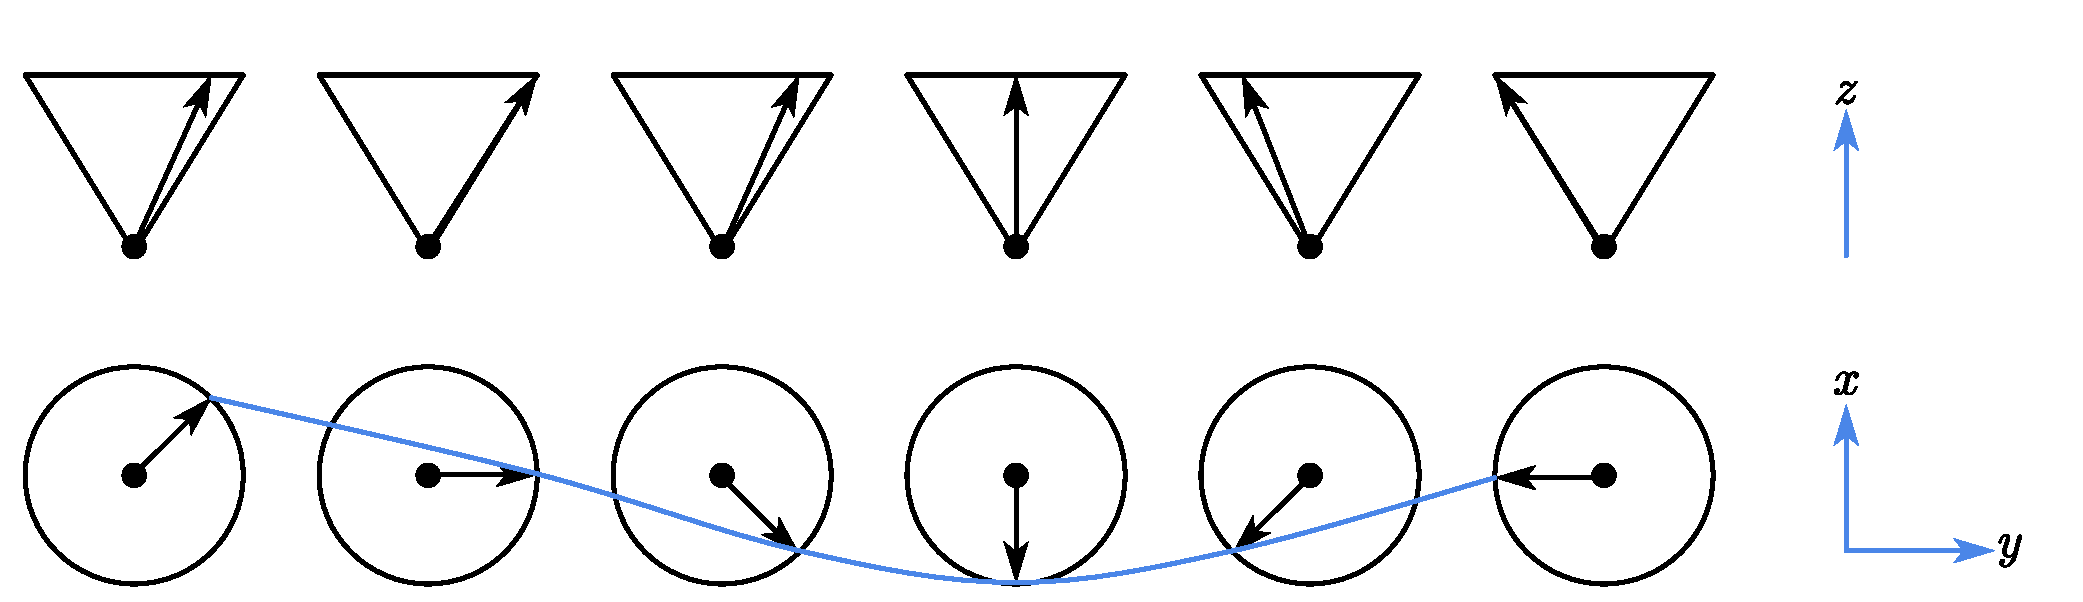
\includegraphics[width=12cm]{figure/spin-wave.pdf}
        \caption{铁磁海森伯模型的自旋波态在 $z$ 方向的投影和在 $x-y$ 平面上的自旋波.}
    \end{figure}
    
在铁磁自旋波理论中, 哈密顿量 
    \begin{equation}
        \hat{H}=E_g+\sum_{k}\omega_{k}\hat{b}_k^\dagger \hat{b}_k^{ },
    \end{equation}
    其中 $\hat{b}_k^\dagger$ 和 $\hat{b}_k^{ }$ 是磁振子的产生消灭算符. 所以应有自旋波理论的基态
    \begin{equation}
        |g\rangle\to |0\rangle,
    \end{equation}
    其中 $|0\rangle$ 代表磁振子的真空态. 这一真空态同时也是 H-P 玻色子算符的真空态, 即 
    \begin{equation}
        \hat{a}_l|0\rangle=0, \quad \hat{b}_{k}|0\rangle=0.
    \end{equation}
    此外, 还可以证明, 在 H-P 变换后, 自旋波态可以写成 
    \begin{equation}
        |\boldsymbol{k}\rangle\to \hat{b}^+_{k}|0\rangle
    \end{equation}
    的形式. 
    \begin{proof}
     \begin{align}
                |\boldsymbol{k}\rangle=&\frac{1}{\sqrt{2SN}}\sum_l\mathrm{e}^{\mathrm{i}\boldsymbol{k}\cdot \boldsymbol{l}}\hat{S}_l^-|g\rangle\nonumber\\
                =&\frac{1}{\sqrt{2SN}}\sum_l\mathrm{e}^{\mathrm{i}\boldsymbol{k}\cdot \boldsymbol{l}}\hat{a}_l^\dagger \sqrt{2S-\hat{a}^\dagger_l \hat{a}_l^{ }}|0\rangle\nonumber\\
                =&\frac{1}{\sqrt{2SN}}\sum_l\mathrm{e}^{\mathrm{i}\boldsymbol{k}\cdot \boldsymbol{l}}\hat{a}_l^\dagger \sqrt{2S}|0\rangle,
            \end{align}
        其中, 第二步到第三步按级数展开的形式理解根号下的算符, 展开式中除了零阶项 $\sqrt{2S}$ 外, 每一项都带有一个消灭算符 $\hat{a}_l$ 在最右边, 利用 $\hat{a}_l|0\rangle=0$, 就只剩下了零阶项. 再利用变换关系
        \begin{equation}
            \hat{b}^\dagger_{k}=\frac{1}{\sqrt{N}}\sum_l\mathrm{e}^{\mathrm{i}\boldsymbol{k}\cdot\boldsymbol{l}}\hat{a}_l^\dagger,
        \end{equation}
        就得到了
        \begin{equation}
            |\boldsymbol{k}\rangle=\hat{b}_{k}^\dagger |0\rangle.
        \end{equation}
    \end{proof}
\end{note}

下面简单讨论一下低温磁化率的计算. 实验中发现磁矩在低温区以 $T^{3 / 2}$ 趋近于饱和, 在临界温度处以 $\sqrt{1-T / T_\mathrm{C}}$ 趋于0(这里 $T_\mathrm{C}$ 为居里温度, 是铁磁和顺磁相变的临界温度). 先考虑总磁矩的计算, 利用H-P变换可以得到:
\begin{align}
\hat{M}^{z}_{\text{tot}} &\equiv g \mu_\mathrm{B} \sum_{l} \hat{S}_{l}^{z} \nonumber\\
&=g \mu_\mathrm{B} \sum_{l}\left(S-\hat{a}_{l}^{\dagger} \hat{a}^{}_{l}\right) \nonumber\\
&=g \mu_\mathrm{B} S N-g \mu_{B} \sum_{l} \hat{a}_{l}^{\dagger} \hat{a}^{}_{l} \nonumber\\
&=M^{z}(0)-g \mu_\mathrm{B} \sum_{k} \hat{b}_{k}^{\dagger} \hat{b}^{}_{k},
\end{align}
其中利用了
\begin{equation}
\sum_{l} \hat{a}_{l}^{\dagger} \hat{a}^{}_{l}=\sum_{k} \hat{b}_{k}^{\dagger} \hat{b}^{}_{k}.
\end{equation}
两边取均值便得到:
\begin{equation}
\left\langle\hat{M}^{z}_{\text{tot}} \right\rangle_{T}=M^{z}_{0}-g \mu_\mathrm{B} \sum_{k}\left\langle\hat{b}_{k}^{\dagger} \hat{b}_{k}^{}\right\rangle_{T}.
\end{equation}

为计算 $\displaystyle\left\langle\hat{b}_{k}^{\dagger} \hat{b}^{}_{k}\right\rangle_{T}$, 可以采用格林函数:
\begin{equation}
G_{k}^\mathrm{R}(t)=-\mathrm{i}\theta(t)\left\langle\left[\hat{b}^{}_{k}(t),\hat{b}_{k}^{\dagger}\right]_{-}\right\rangle_{T}.
\end{equation}
仿照自由电子体系的求解可以得到格林函数的傅里叶变换为:
\begin{equation}
G_{k}^\mathrm{R}(\omega)=\frac{1}{\omega-\omega_{k}+\mathrm{i} \eta},
\end{equation}
利用谱定理可以得到均值 $\left\langle\hat{b}_{k}^{\dagger} \hat{b}_{k}^{}\right\rangle_{T}$ 为:
\begin{equation}
\left\langle\hat{b}_{k}^{\dagger} \hat{b}_{k}^{}\right\rangle_{T} \equiv \int_{-\infty}^{\infty} \frac{-\frac{1}{\pi} \operatorname{Im} G_{k}^\mathrm{R}(\omega)}{\mathrm{e}^{\beta \omega}-1} \mathrm{d} \omega =\frac{1}{\mathrm{e}^{\beta \omega_{k}}-1}.
\end{equation}
这就是自由玻色子的分布函数. 

考虑到自旋波理论只适用于低能态, 类比德拜模型, 可以近似计算:
\begin{equation}\label{HW9}
\sum_{k}\left\langle\hat{b}_{k}^{\dagger} \hat{b}^{}_{k}\right\rangle_{T}\propto T^{3 / 2}.
\end{equation}
这里的 $k$ 属于第一布里渊区. 代回到磁矩均值的表达式中可以得到:
\begin{equation}
\left\langle\hat{M}^{z}(0)\right\rangle_{T}=M^{z}(0)-\alpha T^{3 / 2}.
\end{equation}
$\alpha$ 是前面的系数. 这一结果与实验上得到的结果是符合的, 由布洛赫首次得到, 因此也被称为\textbf{布洛赫 $T^{3 / 2}$ 定律}.

\begin{question}{}{}
证明关系式\eqref{HW9}.
\end{question}


需要注意的是, 虽然采用格林函数计算 $\displaystyle\left\langle\hat{b}_{k}^{\dagger} \hat{b}^{}_{k}\right\rangle_{T}$, 但其并不是格林函数方法, 而仍然是铁磁自旋波近似方法. 下面我们来介绍格林函数方法.

(c) 格林函数理论(考虑$S=1/2$)

格林函数方法适用于任何情况, 但是有时无法严格求解, 所以需要做一些近似. 回到初始时铁磁海森伯模型的哈密顿量:
\begin{equation}
\hat{H}=-J \sum_{l} \sum_{\rho}\left(\hat{S}_{l}^{z} \hat{S}_{l+\rho}^{z}+\hat{S}_{l}^{-} \hat{S}_{l+\rho}^{+}\right) ,
\end{equation}
同样 $z$ 方向的磁矩为:
\begin{equation}
M^{z}(T)=\left\langle\hat{M}^{z}\right\rangle_{T}=g \mu_\mathrm{B} \sum_{l}\left\langle\hat{S}_{l}^{z}\right\rangle_{T}.
\end{equation}
这里我们不考虑自旋波理论中的H-P变换(即不对哈密顿量做近似), 而是通过自旋算符间的关系简化上式. 考虑自旋算符的平方:
\begin{equation}
\hat{\boldsymbol{S}}_{l} \cdot \hat{\boldsymbol{S}}_{l}=\hat{S}_{l}^{z} \hat{S}_{l}^{z}+\frac{1}{2}\left(\hat{S}_{l}^{+} \hat{S}_{l}^{-}+\hat{S}_{l}^{-} \hat{S}_{l}^{+}\right),
\end{equation}
利用升降算符间的对易关系可以得到:
\begin{equation}
\left[\hat{S}_{l}^{+}, \hat{S}_{l}^{-}\right]_{-}=2 \hat{S}_{l}^{z} \Rightarrow \hat{S}_{l}^{+} \hat{S}_{l}^{-}=2 \hat{S}_{l}^{z}+\hat{S}_{l}^{-} \hat{S}_{l}^{+},
\end{equation}
代回到自旋算符的平方中并利用算符恒等式我们得到:
\begin{equation}
\hat{\boldsymbol{S}}_{l} \cdot \hat{\boldsymbol{S}}_{l} =\hat{S}_{l}^{z} \hat{S}_{l}^{z}+\hat{S}_{l}^{z}+\hat{S}_{l}^{-} \hat{S}_{l}^{+}.
\end{equation}
考虑 $(S=1 / 2)$, 有
\begin{equation}
\frac{3}{4} =\frac{1}{4}+\hat{S}_{l}^{z}+\hat{S}_{l}^{-} \hat{S}_{l}^{+} \Rightarrow \hat{S}_{l}^{z} =\frac{1}{2}-\hat{S}_{l}^{-} \hat{S}_{l}^{+} ,
\end{equation}
两边取平均值, 则有
\begin{equation}
\left\langle\hat{S}_{l}^{z}\right\rangle_{T} =\frac{1}{2}-\left\langle\hat{S}_{l}^{-} \hat{S}_{l}^{+}\right\rangle_{T}.
\end{equation}
这样问题就转化为计算 $\left\langle\hat{S}_{l}^{-} \hat{S}_{l}^{+}\right\rangle_{T}$:
\begin{equation}
\left\langle\hat{M}^{z}\right\rangle_{T}=g \mu_\mathrm{B} \sum_{l}\left[\frac{1}{2}-\left\langle\hat{S}_{l}^{-} \hat{S}_{l}^{+}\right\rangle_{T}\right]=M_z(0)-g \mu_\mathrm{B} \sum_{l}\left\langle\hat{S}_{l}^{-} \hat{S}_{l}^{+}\right\rangle_{T}.
\end{equation}

引入如下格林函数:
\begin{equation}
G_{ll}^\mathrm{R}(t)=-\mathrm{i} \theta(t)\left\langle\left[\hat{S}_{l}^{+}(t), \hat{S}_{l}^{-}\right]_{-}\right\rangle_{T} ,
\end{equation}
再通过傅里叶变换, 就可以计算 $G_{ll}^\mathrm{R}(\omega)$. 然后利用谱定理
\begin{equation}
    \langle \hat{S}_l^-\hat{S}_l ^+\rangle_T=\int_{-\infty}^\infty\frac{-\frac{1}{\pi}\mathrm{Im}G_{ll}^{\mathrm{R}}(\omega)}{\mathrm{e}^{\beta\omega}-1}\dd\omega
\end{equation}
计算均值. 

我们先讨论更一般的情况. 考虑如下双时格林函数:
\begin{equation}
G_{l^{\prime} l}^\mathrm{R}(t)=-\mathrm{i} \theta(t)\left\langle\left[\hat{S}_{l^{\prime}}^{+}(t), \hat{S}_{l}^{-}\right]_{-}\right\rangle_{T} .
\end{equation}
当温度 $T=0$ 时, 格林函数要在基态下求平均值, 即
 \begin{align}
        G_{l^{\prime}l}^{\mathrm{R}}(t)=&-\mathrm{i}\theta(t)\left\langle g\left| \left[ \hat{S}_{l^\prime}^+(t),\hat{S}_l^- \right]_- \right|g \right\rangle\nonumber\\
        &=-\mathrm{i}\theta(t)\left\{ \left\langle g\left|\hat{S}^+_{l^\prime}(t)\hat{S}_{l}^- \right| g \right\rangle -\left\langle g \left| \hat{S}_l^-\hat{S}_{l^\prime}^+(t) \right| g \right\rangle \right\},
    \end{align}
其中, 由于自旋上升算符 $\hat{S}^+_{l^\prime}$ 作用在基态 $\displaystyle |g\rangle = \prod_l |S,S\rangle_l$ 上得零, 因此上式第二项取值为零. 在时间 $t>0$ 时, 
 \begin{align}
        \text{第一项}\propto &\left\langle g\left| \hat{S}_{l^\prime}^+(t)\hat{S}_l^- \right| g \right\rangle\nonumber\\
        =&\left\langle g\left| \mathrm{e}^{\mathrm{i}\hat{H}t}\hat{S}_{l^\prime}^+\mathrm{e}^{-\mathrm{i}\hat{H}t}\hat{S}_l^- \right| g \right\rangle\nonumber\\
        =&\mathrm{e}^{\mathrm{i} E_gt}\left\langle g\left| \hat{S}_{l^\prime}^+\mathrm{e}^{-\mathrm{i}\hat{H}t}\hat{S}_l^- \right| g \right\rangle,
    \end{align}
上式的物理含义是, 初始在 $t=0$ 时刻用 $\hat{S}_l^-$ 对基态 $|g\rangle$ 作用一次, 在格点 $l$ 上产生一个自旋缺陷, 经过了 $t$ 时间的演化和传播在 $l^\prime$ 格点上产生缺陷的几率幅. 因此上式相当于一个传播子, 它对时间的傅里叶变换的极点应该能够给出系统元激发的相关结论.
下面利用运动方程法求解这一格林函数. 

对时间求导数, 得到
 \begin{align}
        \mathrm{i}\frac{\dd}{\dd t}G_{l^{\prime} l}^{\mathrm{R}}(t)=&\left( \delta(t)-\eta\theta(t) \right)\left\langle \left[ \hat{S}_{l^\prime}^+(t),\hat{S}_l^- \right]_- \right\rangle_T\nonumber\\
        &-\mathrm{i}\theta(t)\left\langle \left[ \mathrm{i}\frac{\dd}{\dd t}\hat{S}_{l^\prime}^+(t),\hat{S}_l^- \right]_- \right\rangle_T\nonumber\\
        =&\delta(t)\left\langle \left[ \hat{S}_{l^\prime}^+(t),\hat{S}_l^- \right]_- \right\rangle_T-\mathrm{i}\eta G_{l^\prime l}^{\mathrm{R}}(t)\nonumber\\
        &-\mathrm{i}\theta(t)\left\langle \left[ \left[ \hat{S}_{l^\prime}^+(t),\hat{H} \right]_-, \hat{S}_l^- \right]_- \right\rangle_T,
    \end{align}
其中, $\eta=0^+$ 是一个正无穷小量. 根据对易关系, 上式第一项中的均值可以化简成
\begin{equation}
    \left\langle\left[ \hat{S}_{l^\prime}^+(t),\hat{S}_l^- \right]_-\right\rangle_T=\left\langle 2 \hat S_l^z\right\rangle_T \delta_{ll^\prime}.
\end{equation}
运动方程中第三项需要做适当的近似处理, 以使得运动方程闭合. 考虑对易关系:
\begin{align}
        \left[ \hat{S}_{l^\prime}^+(t),\hat{H} \right]_-=&\left[ \mathrm{e}^{\mathrm{i}\hat{H}t}\hat{S}_{l^\prime}^+\mathrm{e}^{-\mathrm{i}\hat{H}t},\hat{H} \right]_-\nonumber\\
        =&\mathrm{e}^{\mathrm{i}\hat{H}t}\left[ \hat{S}_{l^\prime}^+,\hat{H} \right]_-\mathrm{e}^{-\mathrm{i}\hat{H}t}\nonumber\\
        =&\mathrm{e}^{\mathrm{i}\hat{H}t}\left\{ -2J\sum_\rho\left[ \hat{S}_{l^\prime}^z\hat{S}_{l^\prime+\rho}^+-\hat{S}_{l^\prime}^+\hat{S}_{l^\prime+\rho}^z \right] \right\}\mathrm{e}^{-\mathrm{i}\hat{H}t}\nonumber\\
        =&-2J\sum_\rho\left[ \hat{S}_{l^\prime}^z(t)\hat{S}_{l^\prime+\rho}^+(t)-\hat{S}_{l^\prime}^+(t)\hat{S}_{l^\prime+\rho}^z(t) \right],
    \end{align}
代入运动方程的第三项, 得到
\begin{equation}
        \text{第三项}=-2J\sum_\rho \left\{ -\mathrm{i}\theta(t)\left\langle \left[ \hat{S}_{l^\prime}^z(t)\hat{S}_{l^\prime+\rho}^+(t),\hat{S}_l^- \right]_- \right\rangle_T +\mathrm{i}\theta(t)\left\langle \left[ \hat{S}_{l^\prime}^+(t)\hat{S}_{l^\prime+\rho}^z(t),\hat{S}_l^- \right]_- \right\rangle_T \right\},
\end{equation}
为了使上式尽可能地接近格林函数的原始形式, 从而方便求解, 需要作出大胆近似. 1959 年 恰布里科夫(Tyablikov) 提出一种切断近似, 将自旋沿 $z$ 方向分量 $\hat{S}_l^z(t)$ 用其平均值 $\langle \hat{S}_l^z(t) \rangle_T$ 替代. 此外, 由于不同绘景下的力学量平均值相同, 近似处理还可以写成 $\langle \hat{S}_l^z \rangle_T$. 由于格点具有平移对称性, 平均值与指标 $l$ 无关, 因此还可以略去下标. 
\begin{question}{}{}
    验证:
    \begin{equation}
        \left[ \hat{S}_{l^\prime}^+,\hat{H} \right]_-=-2J\sum_\rho\left[ \hat{S}_{l^\prime}^z\hat{S}_{l^\prime+\rho}^+-\hat{S}_{l^\prime}^+\hat{S}_{l^\prime+\rho}^z \right].
    \end{equation}
\end{question}

经过上述处理, 运动方程可以改写为
   \begin{align}
        \mathrm{i}\frac{\dd}{\dd t}G_{l^\prime l}^{\mathrm{R}}(t)=&2\delta(t)\langle \hat{S}^z \rangle_T\delta_{ll^\prime}-\mathrm{i}\eta G_{l^{\prime} l}^{\mathrm{R}}(t)\nonumber\\
        &-2J\langle \hat{S}^z \rangle_T\sum_\rho \left[ G_{l^\prime+\rho,l}^{\mathrm{R}}(t)-G_{l^\prime l }^{\mathrm{R}}(t) \right],
    \end{align}
为处理最后一项中的 $G_{l^\prime+\rho\; l}^{\mathrm{R}}$, 引入对时间的傅里叶变换
\begin{equation}
    G_{l^\prime l}^{\mathrm{R}}(t)=\frac{1}{2\pi}\int_{-\infty}^{\infty}G_{ l^\prime l}^{\mathrm{R}}(\omega)\mathrm{e}^{-\mathrm{i}\omega t}\dd \omega,\quad \delta(t)=\frac{1}{2\pi}\int_{-\infty}^\infty \mathrm{e}^{-\mathrm{i}\omega t}\dd \omega,
\end{equation}
将上式代入, 就得到了频率表象下的格林函数运动方程:
\begin{align}
        \omega G_{l^\prime l}^{\mathrm{R}}(\omega)=&2\langle \hat{S}^z \rangle_T\delta_{ ll^\prime}-\mathrm{i}\eta G_{l^\prime l}^{\mathrm{R}}(\omega)\nonumber\\
        &-2J\langle \hat{S}^z \rangle_T\sum_{\rho}\left[ G_{l^\prime+\rho,l}^\mathrm{R}(\omega)-G_{l^\prime l }^{\mathrm{R}}(\omega) \right].
    \end{align}
考虑到平移不变性, 格林函数 $G_{l^\prime l}$ 是关于变量 $l^\prime-l$ 的函数, 于是可以进一步引入空间点阵的傅里叶变换, 有
\begin{equation}
    \left\{
        \begin{aligned}
            G_{l^\prime l}^{\mathrm{R}}(\omega)&=\frac{1}{N}\sum_{k\in 1\;\mathrm{BZ}} G_k^{\mathrm{R}}(\omega)\mathrm{e}^{\mathrm{i}\boldsymbol{k}\cdot (\boldsymbol{l}^\prime-\boldsymbol{l})},\\
            G_k^{\mathrm{R}}(\omega)&=\sum_{l^\prime -l}G_{l^\prime l }^{\mathrm{R}}(\omega)\mathrm{e}^{-\mathrm{i}\boldsymbol{k}\cdot(\boldsymbol{l}^\prime-\boldsymbol{l})},
        \end{aligned}
    \right.
\end{equation}
于是格林函数变成
\begin{equation}
    G_k^{\mathrm{R}}(\omega)=\frac{2\langle \hat{S}^z \rangle_T}{\omega-\tilde{\omega}_k+\mathrm{i}\eta},
\end{equation}
其中:
\begin{equation}
    \tilde{\omega}_k\equiv 2Jz\langle \hat{S}_z \rangle_T(1-\gamma_k),
\end{equation}
$\gamma_k$ 是结构因子, $\gamma_k=\sum_\rho \mathrm{e}^{\mathrm{i}\boldsymbol{k}\cdot \boldsymbol\rho}/Z$. 根据格林函数的表达式, $\tilde{\omega}_k$ 是 $G_k^{\mathrm{R}}(\omega)$ 的极点实值, 考虑其物理意义, 应该与近似处理后系统的激发能有关.

当温度 $T\to 0$ 时, 自旋沿 $z$ 方向分量应趋于常量, 即 $\langle \hat{S}^z \rangle_T\to S$, 因此有 
\begin{equation}
    \tilde{\omega}_k\to \omega_k=2JZS(1-\gamma_k).
\end{equation}

格林函数的傅里叶变换形式为
 \begin{align}
        G_{l^\prime l }^{\mathrm{R}}(\omega)=&\frac{1}{N}\sum_k G_k^{\mathrm{R}}(\omega)\mathrm{e}^{\mathrm{i}\boldsymbol{k}\cdot (\boldsymbol{l}^\prime -\boldsymbol{l})}\nonumber\\
        =&\frac{1}{N}\sum_k\left[ \frac{2\langle \hat{S}_z \rangle_T}{\omega-\tilde{\omega}_k+\mathrm{i}\eta} \right] \mathrm{e}^{\mathrm{i}\boldsymbol{k}\cdot (\boldsymbol{l}^\prime-\boldsymbol{l})},
    \end{align}
如果取 $l^\prime=l$, 就得到与自旋均值相关的格林函数
\begin{equation}
    G_{ll}^{\mathrm{R}}(\omega)=\frac{1}{N}\sum_k\frac{2\langle \hat{S}_z \rangle_T}{\omega-\tilde{\omega}_k+\mathrm{i}\eta},
\end{equation}
由此可以得到
  \begin{align}
        \left\langle \hat{S}_l^-\hat{S}_l^+ \right\rangle_T=&\int_{-\infty}^\infty\frac{-\frac{1}{\pi}\mathrm{Im}G_{ll}^{\mathrm{R}}(\omega)}{\mathrm{e}^{\beta\omega}-1}\dd\omega\nonumber\\
        =&2\left\langle \hat{S}^z \right\rangle_T\frac{1}{N}\sum_k\int_{-\infty}^{\infty}\frac{\delta(\omega-\tilde{\omega}_k)}{\mathrm{e}^{\beta\omega}-1}\dd\omega\nonumber\\
        =&2\left\langle \hat{S}^z \right\rangle_T\frac{1}{N}\sum_k\frac{1}{\mathrm{e}^{\beta\tilde{\omega}_k}-1},
    \end{align}
其中第二步利用了
\begin{equation}
    \mathrm{Im}G_{ll}^{\mathrm{R}}(\omega)=2\left\langle \hat{S}^z \right\rangle_T\frac{1}{N}\sum_k(-\pi)\delta(\omega-\tilde{\omega}_k).
\end{equation}
这样就得到了算符 $\hat{S}^z$ 平均值的表达式(取 $S=1/2$)
\begin{equation}
    \left\langle \hat{S}^z \right\rangle_T=\frac{1}{2}-2\left\langle \hat{S}^z \right\rangle_T\frac{1}{N}\sum_{k}\frac{1}{\mathrm{e}^{\beta\tilde{\omega}_k}-1},
\end{equation}
由于 $\tilde{\omega}_k$ 中含有 $\langle \hat{S}^z \rangle_T$, 所以这是一个超越方程. 如果引入一个函数
\begin{equation}
    \psi(T)\equiv\frac{1}{N}\sum_k\frac{1}{\mathrm{e}^{\beta\tilde{\omega}_k}-1},
\end{equation}
可以得到形式解
\begin{equation}
    \left\langle \hat{S}^z \right\rangle_T=\frac{1}{2}\frac{1}{ 1+2\psi(T) }.
\end{equation}
上式在取低温和高温极限后, 可以得到解析解, 在中间温度则需要数值求解. 下面考虑低温区和高温区解的情况.

(i) 低温区($T/T_{\mathrm{C}}\ll 1$)

在低温近似下, 有
 \begin{align}
        \tilde \omega_k&=2JZ\left\langle \hat{S}^z \right\rangle_T(1-\gamma_k)\nonumber\\
        &\to 2JZS(1-\gamma_k)\nonumber\\
&\to \omega_k.
    \end{align}
这样, 函数 $\psi(T)$ 变成
\begin{equation}
    \psi(T)=\frac{1}{N}\sum_{k}\frac{1}{\mathrm{e}^{\beta\omega_k}-1}\propto T^{3/2},
\end{equation}
可以作为小量进行展开, $\left\langle\hat{S}^z\right\rangle_T$ 变成
 \begin{align}
        \left\langle \hat{S}^z \right\rangle_T&\approx \frac{1}{2}\left( 1-2\psi(T) \right)\nonumber\\
        &\approx \frac{1}{2}\left( 1-A T^{3/2} \right)\nonumber\\
        &=S\left( 1-A T^{3/2} \right),
    \end{align}
相应地有 $z$ 方向磁矩可以写成
\begin{equation}
    \left\langle \hat{M}^z \right\rangle_T=g\mu_{\mathrm{B}}N\left\langle \hat{S}^z \right\rangle_T =M^z(0)-\alpha T^{3/2},
\end{equation}
其中 $M^z(0)$ 是固有磁矩的值. 这一结果与前面给出的自旋波理论结果一致, 区别仅在于近似方法不同.

(ii) 高温区 ($T_{\mathrm{C}}-T\ll T_{\mathrm{C}}$)

自旋形式解的分母可以用双曲余弦函数写出, 即
  \begin{align}
        1+2\psi(T)&=1+\frac{2}{N}\sum_k\frac{1}{\mathrm{e}^{\beta\tilde{\omega}_k}-1}\nonumber\\
        &=\frac{1}{N}\sum_k\left[ 1+\frac{2}{\mathrm{e}^{\beta\tilde{\omega}_k}-1} \right]\nonumber\\
        &=\frac{1}{N}\sum_k\coth\left( \frac{\beta\tilde{\omega}_k}{2} \right),
    \end{align}
利用双曲余弦的展开式 $\coth x\approx \frac{1}{x}+\frac{x}{3}$, 得到解的近似形式
\begin{equation}
    \left\langle \hat{S}^z \right\rangle_T=\frac{1}{2} \left\{ \frac{1}{N}\sum_k\left[ \frac{2k_{\mathrm{B}}T}{ 2JZ\langle \hat{S}^z \rangle_T(1-\gamma_k)}+\frac{2JZ\langle \hat{S}^z \rangle_T(1-\gamma_k)}{6k_{\mathrm{B}}T} \right] \right\}^{-1},
\end{equation}
其中, 考虑到 
  \begin{align}
        \frac{1}{N}\sum_k\gamma_k&=\frac{1}{N}\sum_k\frac{1}{Z}\sum_\rho \mathrm{e}^{\mathrm{i}\boldsymbol{k}\cdot \boldsymbol{\rho}}\nonumber\\
        &=\frac{1}{NZ}\sum_k\sum_\rho \mathrm{e}^{\mathrm{i}\boldsymbol{k}\cdot \boldsymbol{\rho}}\nonumber\\
        &=\frac{1}{Z}\sum_{\rho}\delta_{\rho,0}\nonumber\\
        &=0,
    \end{align}
再令 
\begin{equation}
    F\equiv \frac{1}{N}\sum_k\frac{1}{1-\gamma_k},
\end{equation}
超越方程就可以写成
\begin{equation}
    \left\langle \hat{S}^z \right\rangle_T=\frac{1}{2}\left( \frac{k_{\mathrm{B}}TF}{JZ\langle \hat{S}^z \rangle_T}+\frac{JZ\langle \hat S^z \rangle_T}{3k_{\mathrm{B}}T} \right)^{-1},
\end{equation}
对等式右边分子分母同乘以 $\left\langle \hat{S}^z \right\rangle_T$, 得到
\begin{equation}
    \left\langle \hat{S}^z \right\rangle_T=\frac{1}{2}\left\langle \hat{S}^z \right\rangle_T \left( \frac{k_{\mathrm{B}}TF}{JZ}+\frac{JZ\langle\hat{S}^z\rangle_T^2}{3k_{\mathrm{B}}T} \right)^{-1},
\end{equation}
可以利用二次式求根公式得到这一方程的解(略去无物理含义的负根), 即
\begin{equation}
    \left\langle \hat{S}^z \right\rangle_T=\sqrt{\left( \frac{1}{2}-\frac{k_{\mathrm{B}}TF}{JZ} \right)\frac{3k_{\mathrm{B}}T}{JZ}}.
\end{equation}

为确定 $T_{\mathrm{C}}$ 的值, 利用 $\left\langle \hat{S}^z \right\rangle_{T=T_{\mathrm{C}}}=0$, 即
\begin{equation}
    \left\langle \hat{S}^z \right\rangle_{T_{\mathrm{C}}}=\sqrt{\left( \frac{1}{2}-\frac{k_{\mathrm{B}}T_{\mathrm{C}}F}{JZ} \right)\frac{3k_{\mathrm{B}}T_{\mathrm{C}}}{JZ}}=0,
\end{equation}
由此解得:
\begin{equation}
    T_{\mathrm{C}}=\frac{JZ}{2k_{\mathrm{B}}F}.
\end{equation}
对 $\langle \hat{S}^z \rangle_T$ 取近似, 取括号外的 $T\to T_{\mathrm{C}}$, 有
 \begin{align}
        \left\langle \hat{S}^z \right\rangle_T&\approx\sqrt{\left[ \frac{1}{2}-\frac{k_{\mathrm{B}}F}{JZ}\left( T-T_{\mathrm{C}}+T_{\mathrm{C}} \right) \right]\frac{3k_{\mathrm{B}}T_{\mathrm{C}}}{JZ}}\nonumber\\
        &=\sqrt{\frac{k_{\mathrm{B}}F}{JZ}\left( T_{\mathrm{C}}-T \right)\frac{3}{2F}}\nonumber\\
        &=\sqrt{\frac{3k_{\mathrm{B}}T_{\mathrm{C}}}{2JZ}\left( 1-\frac{T}{T_{\mathrm{C}}} \right)}.
    \end{align}
\begin{question}{}{}
    证明 $\displaystyle F=\frac{1}{N}\sum_k\frac{1}{1-\gamma_k}$ 在三维情况收敛, 而在一维和二维情况下发散.
\end{question}
\begin{question}{}{}
    证明在低温区:
    \begin{equation}
        \psi(T)=\frac{1}{N}\sum_k\frac{1}{\mathrm{e}^{\beta\omega_k}-1}
    \end{equation}
    在三维情况下收敛, 在一维和二维情况下发散.
\end{question}

\subsection{对反铁磁海森伯模型的应用}
\subsubsection{双子格模型}
当海森伯哈密顿量中 $J<0$ 时, 近邻格点上的自旋趋于反平行排列, 这时可以把晶格分为两个子格, 在每个子格中自旋平行排列与铁磁情况一样, 但两个子格的自旋取向相反, 因此总的自发磁化相互抵消, 这就是反铁磁体的双子格模型:
$$
\begin{array}{cc:cc}
a&b&a&b\\
b&a&b&a\\
\hdashline 
a&b&a&b\\
b&a&b&a
\end{array}
$$
其中 $a$ 子格表示自旋向上, $b$ 子格表示自旋向下.

下面我们从双子格模型出发, 讨论海森伯哈密顿量的基态和激发态. 设每个子格中自旋数为 $N$, 总的磁离子数为 $2 N$, 并取体积 $V=1$ . 则 $\hat H$ 可以用 $a , b$ 两子格的自旋算符表示为:

\begin{align}\label{antiferro-H}
\hat H=&|J| \sum_{i \rho}\left\{\hat{S}_{a i}^{z} \hat{S}_{b, i+\rho}^{z}+\frac{1}{2}\left(\hat{S}_{a i}^{+} \hat{S}_{b, i+\rho}^{-}+\hat{S}_{a i}^{-} \hat{S}_{b, i+\rho}^{+}\right)\right\}\nonumber\\
&+|J| \sum_{j \rho}\left\{\hat{S}_{b j}^{z} \hat{S}_{a, j+\rho}^{z}+\frac{1}{2}\left(\hat{S}_{b j}^{+} \hat{S}_{a, j+\rho}^{-}+\hat{S}_{b j}^{-} \hat{S}_{a, j+\rho}^{+}\right)\right\},
\end{align}
其中 $\hat{\boldsymbol{S}}_{a i}$ 代表子格 $a$ 中 $i$ 格点上自旋算符, $\hat{\boldsymbol{S}}_{b j}$ 为 $b$ 子格中 $j$ 格点上自旋. 
%%%%%%%%%%%%%%%%% 22.4.5 新增内容 %%%%%%%%%%%%%%%%%%%%%%%%%%%%%%%%%%%%%%%%%%%%%%%%%%%%%%%%%%%%%%
\begin{note}
    这里的反铁磁双子格模型哈密顿量的横向分量可以写成更简单的形式:
    \begin{equation}
        \hat H_T=|J|\sum_i\sum_\rho \hat{S}_{ai}^+\hat{S}_{b, i+\rho}^-+|J|\sum_j\sum_\rho \hat{S}_{bj}^+\hat{S}_{a, j+\rho}^-.
    \end{equation}
    \begin{proof}
        在式\eqref{antiferro-H}给出的哈密顿量中, 若对第二项的求和下标做代换, 令 $\boldsymbol{i}+\boldsymbol{\rho}=\boldsymbol{j}$, 有
     \begin{align}
                \sum_i\sum_\rho\hat{S}_{ai}^-\hat{S}_{b, i+\rho}^+=&\sum_i\sum_\rho\hat{S}_{b, i+\rho}^+\hat{S}_{ai}^-\nonumber\\
                =&\sum_j\sum_\rho\hat{S}_{bj}^+\hat{S}_{a, j-\rho}^-\nonumber\\
                =&\sum_j\sum_\rho\hat{S}_{bj}^+\hat{S}_{a, j+\rho}^-,
            \end{align}
        其中, 最后一步利用了近邻格点的中心对称性, 对 $\boldsymbol j+\boldsymbol \rho$ 格点和 $\boldsymbol j-\boldsymbol \rho$ 格点求和相等. 这样, 原来由四项组成的哈密顿量就可以重新归并为两项, 有
        \begin{equation}
            \begin{aligned}
                \hat{H}_T=&\frac{1}{2}|J|\sum_i\sum_\rho{\left(\uline{ \hat{S}_{ai}^+\hat{S}_{b, i+\rho}^-}+\uwave{\hat{S}_{ai}^-\hat{S}_{b, i+\rho}^+ }\right)+\frac{1}{2}|J|\sum_j\sum_\rho\left( \uwave{\hat{S}_{bj}^+\hat{S}_{a, j+\rho}^-} +\uline{\hat{S}_{bj}^-\hat{S}_{a, j+\rho}^+ }\right)}\\
                =&|J|\sum_i\sum_\rho\hat{S}_{ai}^+\hat{S}_{b, i+\rho}^-+|J|\sum_j\sum_\rho\hat{S}_{bj}^+\hat{S}_{a,j+\rho}^-.
            \end{aligned}
        \end{equation} 
    \end{proof}
\end{note}
%%%%%%%%%%%%%%%%%%%%%%%%%%%%%%%%%%%%%%%%%%%%%%%%%%%%%%%%%%%%%%%%%%%%%%%%%%%%%%%%%%%%%%%%%%%%%%%%
假设子格 $a$ 的量子化轴沿 $(+z)$ 方向, $b$ 沿 $(-z)$ 方向, 我们将所有 $a$ 子格中自旋沿 $(+z)$ 向排列, $b$ 中沿 $(-z)$ 向排列的状态称为出发状态 $|\text{Néel}\rangle$:
\begin{equation}
|\text{Néel}\rangle\equiv\prod_{i}|S, S\rangle_{a i} \otimes \prod_{j}|S, -S\rangle_{b j} ,
\end{equation}
有关系
\begin{equation}
\hat{S}_{a i}^{+} |\text{Néel}\rangle=\hat{S}_{b j}^{-} |\text{Néel}\rangle=0,
\end{equation}
说明 $\hat{S}_{a i}^{+}$ 对应于子格 $a$ 中的消灭算符, $\hat{S}_{b j}^{-}$ 对应于子格 $b$ 的消灭算符.

分别定义子格总自旋算符:
\begin{equation}
\hat{\boldsymbol S}_{\mathrm{tot}}^{(a)}=\sum_{i} \hat{\boldsymbol S}_{a i}, \quad\hat{S}_{\mathrm{tot}}^{z(a)}=\sum_{i} \hat{S}_{a i}^{z} ;
\end{equation}
\begin{equation}
\hat{\boldsymbol S}_{\mathrm{tot}}^{(b)}=\sum_{j} \hat{\boldsymbol S}_{b j}, \quad\hat{S}_{\mathrm{tot}}^{z(b)}=\sum_{j} \hat{S}_{b j}^{z} .
\end{equation}
可以得到Néel态是子格总自旋算符的本征态:
\begin{equation}
\hat{S}_{\mathrm{tot}}^{z(a)}|\text{Néel}\rangle=N S|\text{Néel}\rangle, \quad\hat{S}_{\mathrm{tot}}^{z(b)}|\text{Néel}\rangle=-N S|\text{Néel}\rangle.
\end{equation}
但遗憾的是 Néel 态并不是哈密顿量的严格本征态, 因为:
\begin{equation}
\left[\hat{H},\hat{S}_{\mathrm{tot}}^{z(a, b)}\right] _-\neq 0 .
\end{equation}

为了确定反铁磁海森堡模型的基态, 我们首先要确定基态能的范围. 根据变分法, 哈密顿量在任意态下的均值一定大于等于基态能, 这里可以用哈密顿量在 Néel 态下的均值作为基态能上限:
\begin{equation}\label{neelsx}
\langle\text{Néel}|\hat{H}|\text{Néel}\rangle=-2 N Z|J| S^{2} .
\end{equation}
\begin{question}{}{}
    证明式\eqref{neelsx}.
\end{question}

参考 PW. Anderson. phys. Rev. 83(1951)1260, Anderson 给出了基态能下限为: $\displaystyle -2 N Z|J| S^{2}\left(1+\frac{1}{Z S}\right)$. 最终可以得到反铁磁基态能在如下范围内:
\begin{equation}
-2 N Z|J| S^{2}\left(1+\frac{1}{Z S}\right)<E_{g}<-2 N Z|J| S^{2}.
\end{equation}
特别地, 当 $S=1 / 2$, 体系是简单立方晶格 $(Z=6)$ 时, 反铁磁基态能在如下范围:
\begin{equation}
-2 N Z|J| \frac{1}{3}<E_{g}<-2 N Z|J| \frac{1}{4}.
\end{equation}

下面分别用自旋波理论和格林函数理论讨论反铁磁海森堡模型.

\subsubsection{反铁磁海森伯模型的若干理论结果}
(a) 反铁磁自旋波理论

该节参考 R. Kubo. Phys. Rev. 87. (1957)568.

分别对两个子格引入玻色子算符 $\hat{a}^{}_{i}, \hat{a}_{i}^{\dagger}, \hat{b}^{}_{j}, \hat{b}_{j}^{\dagger}$, 满足
\begin{equation}
\left[\hat{a}^{}_{i}, \hat{a}_{j}^{\dagger}\right]_-=\delta_{i j}, \quad\left[\hat{a}_{i}, \hat{a}_{j}\right]_-=\left[\hat{a}_{i}^{\dagger}, \hat{a}_{j}^{\dagger}\right]_-=0;
\end{equation}
\begin{equation}
\left[\hat{b}^{}_{i}, \hat{b}_{j}^{\dagger}\right]_-=\delta_{i j}, \quad\left[\hat{b}_{i}, \hat{b}_{j}\right]_-=\left[\hat{b}_{i}^{\dagger}, \hat{b}_{j}^{\dagger}\right]_-=0;
\end{equation}
\begin{equation}
\left[\hat{a}^{}_{i}, \hat{b}_{j}^{}\right]_-=\left[\hat{a}^{\dagger}_{i}, \hat{b}^{}_{j}\right]_-=\left[\hat{a}_{i}^{}, \hat{b}_{j}^{\dagger}\right]_-=\left[\hat{a}_{i}^{\dagger}, \hat{b}_{j}^{\dagger}\right]_-=0.
\end{equation}
由于 $a$ 子格自旋朝上, 可仿铁磁情况作 H-P 变换, 引入子格 $a$ 的产生及消灭算符
\begin{equation}
\left\{\begin{array}{l}
\hat{S}_{a i}^{+}=\left(\sqrt{2 S-\hat a_{i}^{\dagger} \hat a^{}_{i}}\right) \hat a^{}_{i}\approx \sqrt{2 S} \hat{a}_{i},\\
\hat{S}_{a i}^{-}=\hat a_{i}^{\dagger} \sqrt{2 S-\hat a_{i}^{\dagger} \hat a^{}_{i}} \approx \sqrt{2 S} \hat{a}_{i}^{\dagger} ,\\
\hat{S}_{a i}^{z}=S-\hat a_{i}^{\dagger} \hat a^{}_{i}.
\end{array}\right.
\end{equation}
对于 $b$ 子格 $\hat{S}^{+}$ 与 $\hat{S}^{-}$ 的作用将颠倒, 应定义
\begin{equation}
\left\{\begin{array}{l}
\hat{S}_{b j}^{+}=\hat b_{j}^{\dagger} \sqrt{2 S-\hat b_{j}^{\dagger} \hat b^{}_{j}}\approx \sqrt{2 S} \hat{b}_{j}^{\dagger}, \\
\hat{S}_{b j}^{-}=\left(\sqrt{2 S-\hat b_{j}^{\dagger} \hat b^{}_{j}}\right) \hat b^{}_{j}\approx \sqrt{2 S} \hat{b}_{j}, \\
\hat{S}_{b j}^{z}=\hat b_{j}^{\dagger} \hat b^{}_{j}-S.
\end{array}\right.
\end{equation}
代入哈密顿量, 并略去算符的四次项, 求得低温近似的哈密顿量:
\begin{align}
\hat H=&-2 N Z S^{2}|J|+2 Z S|J|\left(\sum_{i} \hat a_{i}^{\dagger} \hat a^{}_{i}+\sum_{j} \hat b_{j}^{\dagger} \hat b^{}_{j}\right)\nonumber\\
&+2|J| S \sum_{i, \rho}\left(\hat a^{}_{i} \hat b^{}_{i+\rho}+\hat a_{i}^{\dagger} \hat b_{i+\rho}^{\dagger}\right),
\end{align}
其中 $N$ 为子格中自旋数. 

引入傅里叶变换(平面波展开):
\begin{equation}
\left\{\begin{aligned}
&\hat{a}_{i}=\frac{1}{\sqrt{N}} \sum_{k} \hat{a}_{k} \e^{\mathrm{i} \boldsymbol{k} \cdot \boldsymbol{i}}, \\
&\hat{a}_{i}^{\dagger}=\frac{1}{\sqrt{N}} \sum_{k} \hat{a}_{k}^{\dagger} \e^{-\mathrm{i} \boldsymbol{k} \cdot \boldsymbol{i}},
\end{aligned}\right.
\end{equation}
和
\begin{equation}
\left\{\begin{aligned}
&\hat{b}_{j}=\frac{1}{\sqrt{N}} \sum_{k} \hat{b}_{k} \e^{\mathrm{i} \boldsymbol{k} \cdot \boldsymbol{j}},\\
&\hat{b}_{j}^{\dagger}=\frac{1}{\sqrt{N}} \sum_{k} \hat{b}_{k}^{\dagger} \e^{-\mathrm{i} \boldsymbol{k} \cdot \boldsymbol{j}},
\end{aligned}\right.
\end{equation}
可以证明 $\hat{a}^{}_{k}, \hat{a}_{k}^{\dagger}, \hat{b}^{}_{k}, \hat{b}_{k}^{\dagger}$ 也满足玻色子对易关系. 这样反铁磁海森堡模型的哈密顿量可以化为:
\begin{align}
\hat{H}=&-2 N Z|J| S^{2}+2 Z S|J| \sum_{k}\left(\hat{a}_{k}^{\dagger} \hat{a}^{}_{k}+\hat{b}_{k}^{\dagger} \hat{b}^{}_{k}\right) \nonumber\\
&+2 Z S|J| \sum_{k} \gamma_{k}\left(\hat{a}_{k} \hat{b}_{k}+\hat{b}_{k}^{\dagger} \hat{a}_{k}^{\dagger}\right) ,
\end{align}
其中略去了高阶项. 上式中第一项是出发状态的能量, 第二项代表各子格中自旋波, 第三项为交叉项代表两子格自旋波的相互作用. 该式说明本征模式应当是两个子格自旋波的组合. 下面用Bogoliubov变换方法及格林函数方法处理这个近似哈密顿量.

1. Bogoliubov变换方法

Bogoliubov变换的本质思想是引入组合的自旋波算符, 消除交叉项, 使 $\hat H$ 对角化.

第一步: 考虑如何组合两个子格中的自旋波算符. 先考察子格算符的运动方程:
\begin{equation}
\left\{\begin{aligned}
&\mathrm{i} \frac{\dd}{\dd t}\hat{a}_{k}(t)=\left[\hat a_{k}(t),\hat H\right]_-=\e^{\mathrm{i}\hat{H}t}\left[\hat a_{k},\hat H\right]_- \e^{-\mathrm{i}\hat{H}t}=\e^{\mathrm{i}\hat{H}t} \left[  2 Z S|J|\left(\hat a_{k}+\gamma^{}_{k} \hat b_{k}^{\dagger}\right) \right] \e^{-\mathrm{i}\hat{H}t},\\
&\mathrm{i} \frac{\dd}{\dd t}\hat{b}_{k}(t)=\left[\hat b_{k}(t),\hat H\right]_-=\e^{\mathrm{i}\hat{H}t}\left[\hat b_{k},\hat H\right]_- \e^{-\mathrm{i}\hat{H}t}=\e^{\mathrm{i}\hat{H}t} \left[  2 Z S|J|\left(\hat b_{k}+\gamma^{}_{k} \hat a_{k}^{\dagger}\right) \right] \e^{-\mathrm{i}\hat{H}t}.
\end{aligned}\right.
\end{equation}
上式说明, 应当组合 $\hat a^{}_{k}$ 与 $\hat b_{k}^{\dagger}$ 以及 $\hat b^{}_{k}$ 与 $\hat a_{k}^{\dagger}$ 构成两套新的自旋波算符 $\hat \alpha_{k}$ 和 $\hat \beta_{k}$:
\begin{equation}
\left\{\begin{aligned}
&\hat \alpha^{}_{k}=u^{}_{k} \hat a^{}_{k}-v^{}_{k} \hat b_{k}^{\dagger}, & \hat \alpha_{k}^{\dagger}=u^{}_{k} \hat a_{k}^{\dagger}-v^{}_{k} \hat b^{}_{k}, \\
&\hat \beta^{}_{k}=u^{}_{k} \hat b^{}_{k}-v^{}_{k} \hat a_{k}^{\dagger}, & \hat \beta_{k}^{\dagger}=u^{}_{k} \hat b_{k}^{\dagger}-v^{}_{k} \hat a^{}_{k}.
\end{aligned}\right.
\end{equation}
这里 $u_{k}$ 和 $v_{k}$ 设为实函数, 上式为正则变换. 应当指出, 作正则变换时要保证所有的对易关系在形式上不改变, 这是检验变换式的一个重要物理条件.

第二步: 要求变换后新算符仍满足玻色对易式, 即
\begin{equation}
\left[\hat \alpha^{}_{k}, \hat \alpha_{k^{\prime}}^{\dagger}\right]_-=\delta_{k k^{\prime}},\left[\hat \beta^{}_{k}, \hat \beta_{k^{\prime}}^{\dagger}\right]_-=\delta_{k k^{\prime}},
\end{equation}
\begin{equation}
\left[\hat \alpha_{k}, \hat \beta_{k^{\prime}}\right]_-=\left[\hat \alpha^{}_{k}, \hat \beta_{k^{\prime}}^{\dagger}\right]_-=\left[\hat \alpha_{k}^{\dagger}, \hat \beta^{}_{k^{\prime}}\right]_-=\left[\hat \alpha_{k}^{\dagger}, \hat \beta_{k^{\prime}}^{\dagger}\right]_-=0.
\end{equation}

用 $\left[\hat \alpha^{}_{k}, \hat \alpha_{k^{\prime}}^{\dagger}\right]_-=\delta_{k k^{\prime}}$ 举例. 将上面的变换代入, 可得:
\begin{align}
\left[\hat \alpha^{}_{k}, \hat \alpha_{k^{\prime}}^{\dagger}\right]_-&=\left[u_{k} \hat a_{k}-v^{}_{k} \hat b_{k}^{\dagger}, u^{}_{k^{\prime}} \hat a_{k^{\prime}}^{\dagger}-v_{k^{\prime}} \hat b_{k^{\prime}}\right]_-\nonumber\\
&=u_{k}u_{k^{\prime}}\left[\hat a^{}_{k}, \hat a_{k^{\prime}}^{\dagger}\right]_- + v_{k}v_{k^{\prime}}\left[\hat b^{\dagger}_{k}, \hat b^{}_{k^{\prime}}\right]_-\nonumber\\
&=u_{k}u_{k^{\prime}}\delta_{k k^{\prime}}+v_{k}v_{k^{\prime}}(-\delta_{k k^{\prime}})\nonumber\\
&=(u_{k}^2-v_{k}^2)\delta_{k k^{\prime}}\nonumber\\
&=\delta_{k k^{\prime}},
\end{align}
即可求得 $u_{k}$ 与 $v_{k}$ 的一个关系式:
\begin{equation}
u_{k}^{2}-v_{k}^{2}=1.
\end{equation}

利用上式可以写出逆变换:
\begin{equation}
\left\{\begin{aligned}
&\hat a^{}_{k}=u^{}_{k} \hat \alpha^{}_{k}+v_{k} \hat \beta_{k}^{\dagger}, & \hat a_{k}^{\dagger}=u^{}_{k} \hat \alpha_{k}^{\dagger}+v^{}_{k} \hat \beta^{}_{k} ,\\
&\hat b^{}_{k}=u^{}_{k} \hat \beta^{}_{k}+v_{k} \hat \alpha_{k}^{\dagger}, & \hat b_{k}^{\dagger}=u^{}_{k} \hat \beta_{k}^{\dagger}+v^{}_{k} \hat \alpha^{}_{k}.
\end{aligned}\right.
\end{equation}

第三步: 要求用新算符 $\hat \alpha_{k},\hat \beta_{k}$ 表示的哈密顿量 $\hat H$ 对角化, 将得到 $u_{k}$ 与 $v_{k}$ 的另一个关系式, 从而具体解出 $u_{k}$ 与 $v_{k}$. 

将逆变换代入哈密顿量表达式, 得:
\begin{align}
\hat H=&-2 N Z|J| S(S+1)\nonumber\\
&+ 2 Z|J| S \sum_{k}\left\{\left(u_{k}^{2}+v_{k}^{2}+2 \gamma_{k} u_{k} v_{k}\right)\left(\hat \alpha_{k}^{\dagger} \hat \alpha^{}_{k}+\hat \beta_{k}^{\dagger} \hat \beta^{}_{k}+1\right)\right.\nonumber\\
&+\left.\left[\left(u_{k}^{2}+v_{k}^{2}\right) \gamma_{k}+2 u_{k} v_{k}\right]\left(\hat \alpha_{k} \hat \beta_{k}+\hat \alpha_{k}^{\dagger} \hat \beta_{k}^{\dagger}\right)\right\}.
\end{align}
为使 $\hat H$ 对角化, 要求非对角项 $\left(\hat \alpha_{k} \hat \beta_{k}+\hat \alpha_{k}^{\dagger} \hat \beta_{k}^{\dagger}\right)$ 的系数等于零, 即
\begin{equation}
\left(u_{k}^{2}+v_{k}^{2}\right) \gamma_{k}+2 u_{k} v_{k}=0.
\end{equation}
上式与$u_{k}^{2}-v_{k}^{2}=1$联立可解出
\begin{align}
&u_{k}^{2}=\frac{1}{2}(1+\Delta), \\
&v_{k}^{2}=-\frac{1}{2}(1-\Delta), \\
&\Delta=\frac{1}{\sqrt{1-\gamma_{k}^{2}}}.
\end{align}
将此结果代入, 求得对角化哈密顿量
\begin{align}
\hat H=&-2 N Z|J| S(S+1)+ \sum_{k}\omega_{k}\left(\hat \alpha_{k}^{\dagger} \hat \alpha^{}_{k}+\hat \beta_{k}^{\dagger} \hat \beta^{}_{k}+1\right)\nonumber\\
=&E_0+\sum_{k}\omega_{k}\left(\hat \alpha_{k}^{\dagger} \hat \alpha^{}_{k}+\hat \beta_{k}^{\dagger} \hat \beta^{}_{k}\right)\nonumber\\
=&E_0+\sum_{k}\omega_{k}\left(\hat n_{\alpha_{k}}+\hat n_{\beta_{k}}\right),
\end{align}
其中 $\displaystyle E_0=-2 N Z|J| S(S+1)+ \sum_{k}\omega_{k}$ 为常数. 这里的$\omega_{k}$ 代表反铁磁自旋波量子:
\begin{equation}
\omega_{k}\equiv 2 Z|J| S \sqrt{1-\gamma_{k}^{2}}.
\end{equation}
可以看出, 对于每个 $\boldsymbol{k}$ 存在两支简并的反铁磁自旋波, 分别由 $\hat \alpha_{k}^{\dagger} \hat \alpha^{}_{k}$ 和 $\hat \beta_{k}^{\dagger} \hat \beta^{}_{k}$ 代表其准粒子数算符, 记为 $\hat n_{\alpha_{k}}$ 和 $\hat n_{\beta_{k}}$.

将反铁磁自旋波哈密顿量作用到本征态 $|E\rangle$ 上, 有本征方程
\begin{equation}
\hat H |E\rangle=E |E\rangle.
\end{equation}
可在粒子数表象下标记 $|E\rangle$:
\begin{equation}
|E\rangle=\left|\left\{ n_{\alpha_{k}},n_{\beta_{k}}\right\}\right\rangle.
\end{equation}
对于磁振子真空态 $|0\rangle$, 有
\begin{equation}
\hat \alpha_{k}|0\rangle=0,\quad \hat \beta_{k}|0\rangle=0, \quad\langle 0| 0\rangle=\mathbbm{1}.
\end{equation}
则
\begin{equation}
|E\rangle=\left|\left\{ n_{\alpha_{k}},n_{\beta_{k}}\right\}\right\rangle=\prod_{k}\frac{\left(\hat\alpha_{k}^{\dagger}\right)^{n_{\alpha_{k}}}}{\sqrt{n_{\alpha_{k}}!}}\frac{\left(\hat\beta_{k}^{\dagger}\right)^{n_{\beta_{k}}}}{\sqrt{n_{\beta_{k}}!}}|0\rangle.
\end{equation}

现在讨论反铁磁体的基态. 基态能量 $E_{0}$ 应当是无准粒子激发时 $\hat H$ 的本征值:
\begin{equation}
E_{g}=E_{0} =-2 N Z|J| S(S+1)+ \sum_{k}\omega_{k}=-2 N Z|J| S(S+\lambda),
\end{equation}
其中
\begin{equation}
\lambda=\frac{1}{N} \sum_{k}\left(1-\sqrt{1-\gamma_{k}^{2}}\right).
\end{equation}
由于 $\left|\gamma_{k}\right|< 1$, 故 $0 < \lambda < 1$. 反铁磁体的基态能量介乎出发状态 $|\text{Néel}\rangle$ 的能量 $\left(-2 N Z|J| S^{2}\right)$ 与 $-2 N Z|J| S(S+1)$ 之间. 下面我们以简单立方为例验证这点.对简单立方, 考虑 $S=1/2$, 配位数 $Z=6$, $\lambda=0.097\approx 0.1$, 则
\begin{equation}
E_{g}=-2 N Z|J| S(S+\lambda)=-2 N Z|J|\frac{3}{10}.
\end{equation}
这个数据在前面得到的 $\displaystyle -2 N Z|J| \frac{1}{3}< E_{g}< -2 N Z|J| \frac{1}{4}$ 范围中. 可以看到, 基态并不完全像双子格模型所建议的磁有序状态. 在基态每一子格中自旋不是完全平行的, 而是存在着取向的不一致性.

下面讨论 $a$ 子格的饱和磁化强度. 总自旋的 $z$ 分量算符可表示为
\begin{align}
\hat{S}_\mathrm{tot}^{z(a)} & \equiv \sum_{i=1}^{N} \hat{S}_{a i}^{z}=\sum_{i=1}^{N}\left(S-\hat a_{i}^{\dagger} \hat a^{}_{i}\right)=N S-\sum_{k} \hat a_{k}^{\dagger} \hat a^{}_{k}\nonumber \\
&=NS-\sum_{k}\left[u_{k}^{2} \hat \alpha_{k}^{\dagger} \hat \alpha^{}_{k}+v_{k}^{2} \hat \beta^{}_{k} \hat \beta_{k}^{\dagger}+u_{k} v_{k}\left(\hat \alpha_{k} \hat \beta_{k}+\hat \alpha_{k}^{\dagger} \hat \beta_{k}^{\dagger}\right)\right],
\end{align}
则基态 $a$ 子格自旋平均值为
\begin{align}
&\left\langle0\left|\hat{S}_\mathrm{tot}^{z(a)} \right|0\right\rangle \nonumber\\
=&NS-\sum_{k}\left\langle0\left|\left[u_{k}^{2} \hat \alpha_{k}^{\dagger} \hat \alpha^{}_{k}+v_{k}^{2} \hat \beta^{}_{k} \hat \beta_{k}^{\dagger}+u_{k} v_{k}\left(\hat \alpha_{k} \hat \beta_{k}+\hat \alpha_{k}^{\dagger} \hat \beta_{k}^{\dagger}\right)\right] \right|0\right\rangle \nonumber\\
=&NS- \sum_{k} v_{k}^{2}\left\langle0\left|\hat \beta^{}_{k} \hat \beta_{k}^{\dagger}\right|0\right\rangle\nonumber \\
=&NS-\sum_{k} v_{k}^{2}\nonumber\\
=&N\left[S+\frac{1}{N}\sum_{k}\frac{1}{2}\left(1-\frac{1}{\sqrt{1-\gamma_{k}^{2}}}\right)\right].
\end{align}
上式右边第一项代表子格 $a$ 中所有自旋取向完全一致时的贡献, 对应于子格的饱和磁化. 第二项为子格中自旋取向的平均偏离量. Anderson算出对于简单立方晶格, 有
\begin{equation}
\left\langle0\left|\hat{S}_\mathrm{tot}^{z(a)} \right|0\right\rangle=N[S-0.078],
\end{equation}
其中 $-0.078$ 来自量子效应. 由此可知在基态中子格的自旋并非绝对取向一致, 而是相对饱和值 $N S$ 有少量的平均偏离, 这种取向的无序性与反铁磁体中自旋波量子的零点运动有关. 

零温情况下, 磁矩
\begin{equation}
M_{\mathrm{tot}}^{z(a)}(0) =g \mu_{\mathrm{B}} N\left[S+\frac{1}{N} \sum_{k} \frac{1}{2}\left(1-\frac{1}{\sqrt{1-\gamma_{k}^{2}}}\right)\right].
\end{equation}

下面考虑有限温度(接近0 K), 此时 
\begin{align}
        M_{\mathrm{tot}}^{z(a)}(T)&=g \mu_{\mathrm{B}} \sum_{i}\left\langle\hat{S}_{a i}^{z}\right\rangle_{T}=g \mu_{\mathrm{B}} \sum_{i}\left({S}-\left\langle\hat{a}_{i}^{\dagger} \hat{a}^{}_{i}\right\rangle_{T}\right) \nonumber\\
        &=g \mu_{\mathrm{B}} N S-g \mu_{\mathrm{B}} \sum_{k}\left\langle\hat{a}_{k}^{\dagger} \hat{a}^{}_{k}\right\rangle_{T}\nonumber\\
        &=g \mu_{\mathrm{B}} N S-g \mu_{\mathrm{B}} \sum_{k}\left[u_{k}^{2}\left\langle\hat{\alpha}_{k}^{\dagger} \hat{\alpha}^{}_{k}\right\rangle_{T}+v_{k}^{2}\left\langle\hat{\beta}_{k}^{} \hat{\beta}^{\dagger}_{k}\right\rangle_{T}\right.\nonumber\\
        &\qquad\qquad\qquad\qquad\qquad \left.+u_{k}^{}v_{k}^{}\left(\left\langle\hat{\alpha}_{k}^{} \hat{\beta}^{}_{k}\right\rangle_{T}+\left\langle\hat{\alpha}_{k}^{\dagger} \hat{\beta}^{\dagger}_{k}\right\rangle_{T}\right)\right].
        \end{align}
由于 $\hat{\alpha}_{k}$ 和 $\hat{\beta}_{k}$ 均为玻色算符, 对应的激发量子平均数服从玻色分布, 有:
\begin{equation}
\left\langle\hat{\alpha}_{k}^{\dagger} \hat{\alpha}^{}_{k}\right\rangle_{T}=\frac{1}{\e^{\beta\omega_{k}}-1},\quad
\left\langle\hat{\beta}_{k}^{} \hat{\beta}^{\dagger}_{k}\right\rangle_{T}=1+\frac{1}{\e^{\beta\omega_{k}}-1},\quad
\left\langle\hat{\alpha}_{k}^{} \hat{\beta}^{}_{k}\right\rangle_{T}=\left\langle\hat{\alpha}_{k}^{\dagger} \hat{\beta}^{\dagger}_{k}\right\rangle_{T}=0,
\end{equation}
则
\begin{align}
M_{\mathrm{tot}}^{z(a)}(T)&=g \mu_{\mathrm{B}} N S-g \mu_{\mathrm{B}} \sum_{k}\left[u_{k}^{2}\left\langle\hat{\alpha}_{k}^{\dagger} \hat{\alpha}^{}_{k}\right\rangle_{T}+v_{k}^{2}\left\langle\hat{\beta}_{k}^{} \hat{\beta}^{\dagger}_{k}\right\rangle_{T}\right]\nonumber\\
&\approx M_{\mathrm{tot}}^{z(a)}(0)-g \mu_{\mathrm{B}}\sum_{k}u_{k}^{2}\left\langle\hat{\alpha}_{k}^{\dagger} \hat{\alpha}^{}_{k}\right\rangle_{T}\nonumber\\
&=M_{\mathrm{tot}}^{z(a)}(0)-g \mu_{\mathrm{B}}\sum_{k}\frac{u_{k}^{2}}{\e^{\beta\omega_{k}}-1}.
\end{align}
注意到 $\displaystyle\lim _{k \rightarrow 0}\gamma_k =1-ak^2$, 在 $k \rightarrow 0$ 时, $\omega_{k}$ 有如下渐进性质:
\begin{equation}
\lim _{k \rightarrow 0} \omega_{k}\propto \lim _{k \rightarrow 0}  \sqrt{\left(1-\gamma_{k}\right)\left(1+\gamma_{k}\right)} \sim  k \lim _{k \rightarrow 0} \sqrt{1+\gamma_{k}} \sim k,
\end{equation}
则
\begin{equation}
\sum_{k} \frac{u^2_{k}}{\e^{\beta \omega_{k}}-1} \sim \sum_{k} \frac{1+1 /(C k)}{\e^{C \beta k}-1} \sim \int \frac{k \mathrm{d} k}{\e^{C\beta k}} \propto T^{2},
\end{equation}
其中 $C$ 为一常数. 最终的磁矩表达式可以写为:
\begin{equation}
M_{\mathrm{tot}}^{z(a)}(T)=M_{\mathrm{tot}}^{z(a)}(0)-\alpha T^{2},
\end{equation}
其中 $\alpha$ 为比例系数.


2. 格林函数方法

回到近似哈密顿量
\begin{align}
\hat{H}=&-2 N Z|J| S^{2}+2 Z S|J| \sum_{k}\left(\hat{a}_{k}^{\dagger} \hat{a}^{}_{k}+\hat{b}_{k}^{\dagger} \hat{b}^{}_{k}\right) \nonumber\\
&+2 Z S|J| \sum_{k} \gamma_{k}\left(\hat{a}_{k} \hat{b}_{k}+\hat{b}_{k}^{\dagger} \hat{a}_{k}^{\dagger}\right) .
\end{align}

考虑 $a$ 子格的磁矩 $M_{\mathrm{tot}}^{z(a)}(T)$. 参考铁磁自旋波理论中磁矩的计算, 可以得到:
\begin{align}
M_{\mathrm{tot}}^{z(a)}(T)&=g \mu_{\mathrm{B}} \sum_{i}\left\langle\hat{S}_{a i}^{z}\right\rangle_{T}=g \mu_{\mathrm{B}} \sum_{i}\left({S}-\left\langle\hat{a}_{i}^{\dagger} \hat{a}^{}_{i}\right\rangle_{T}\right) \nonumber\\
&=g \mu_{\mathrm{B}} N S-g \mu_{\mathrm{B}} \sum_{k}\left\langle\hat{a}_{k}^{\dagger} \hat{a}^{}_{k}\right\rangle_{T}.
\end{align}
可以利用格林函数法计算 $\left\langle\hat{a}_{k}^{\dagger} \hat{a}^{}_{k}\right\rangle_{T}$, 为此需引入如下格林函数:
\begin{equation}
G_{k}^\mathrm{R}(t)=-\mathrm{i} \theta(t)\left\langle\left[\hat{a}^{}_{k}(t), \hat{a}_{k}^{\dagger}\right]_-\right\rangle_{T},
\end{equation}
运动方程:
\begin{equation}
\mathrm{i} \frac{\mathrm{d}}{\mathrm{d} t} G_{k}^\mathrm{R}(t)=[\delta(t)-\eta \theta(t)]\left\langle\left[\hat{a}^{}_{k}(t), \hat{a}_{k}^{\dagger}\right]_-\right\rangle_{T}-\mathrm{i} \theta(t)\left\langle\left[\mathrm{i} \frac{\mathrm{d}}{\mathrm{d} t} \hat{a}^{}_{k}(t), \hat{a}_{k}^{\dagger}\right]_-\right\rangle_{T}.
\end{equation}
其中计算 $\displaystyle\mathrm{i} \frac{\mathrm{d}}{\mathrm{d} t} \hat{a}_{k}(t)$ 时, 需要计算如下对易关系:
\begin{align}
{\left[\hat{a}_{k}, \hat{H}\right]_- } &=2 Z S|J| \sum_{k^{\prime}}\left[\hat{a}^{}_{k}, \hat{a}_{k^{\prime}}^{\dagger} \hat{a}^{}_{k^{\prime}}\right]_-+2 Z S|J| \sum_{k^{\prime}} \gamma^{}_{k^{\prime}}\left[\hat{a}^{}_{k}, \hat{b}_{k^{\prime}}^{\dagger} \hat{a}_{k^{\prime}}^{\dagger}\right]_- \nonumber\\
&=2 Z S|J| \sum_{k^{\prime}}\left(\hat{a}^{}_{k^{\prime}} \delta^{}_{k k^{\prime}}+\gamma^{}_{k^{\prime}} \hat{b}_{k^{\prime}}^{\dagger} \delta^{}_{k k^{\prime}}\right) \nonumber\\
&=2 Z S|J|\left(\hat{a}^{}_{k}+\gamma^{}_{k} \hat{b}_{k}^{\dagger}\right) .
\end{align}
代回到运动方程中我们得到:
\begin{align}
\mathrm{i} \frac{\mathrm{d}}{\mathrm{d} t} G_{k}^\mathrm{R}(t) &=[\delta(t)-\eta \theta(t)]\left\langle\left[\hat{a}^{}_{k}(t), \hat{a}_{k}^{\dagger}\right]_-\right\rangle_{T}-\mathrm{i} 2 Z S|J| \theta(t)\left\langle\left[\hat a^{}_{k}(t)+\gamma^{}_{k}\hat b_{k}^{\dagger}(t), \hat{a}_{k}^{\dagger}\right]_-\right\rangle_{T}\nonumber \\
&=\delta(t)\left\langle\left[\hat{a}^{}_{k}(t), \hat{a}_{k}^{\dagger}\right]_-\right\rangle_{T}-\ii\eta G_{k}^\mathrm{R}(t)+2 Z S|J| G_{k}^\mathrm{R}(t)+2 Z S|J| \gamma_{k} F_{k}^\mathrm{R}(t) \nonumber\\
&=\delta(t)+(2 Z S|J|-\mathrm{i} \eta) G_{k}^\mathrm{R}(t)+2 Z S|J| \gamma_{k} F_{k}^\mathrm{R}(t),
\end{align}
其中引入了额外的格林函数:
\begin{equation}
F_{k}^\mathrm{R}(t)=-\mathrm{i} \theta(t)\left\langle\left[ \hat b_{k}^{\dagger}(t), \hat{a}_{k}^{\dagger}\right]_-\right\rangle_{T} .
\end{equation}
同样地, 我们可以得到 $F_{k}^\mathrm{R}(t)$ 的运动方程:
\begin{equation}
\mathrm{i} \frac{\mathrm{d}}{\mathrm{d} t} F_{k}^\mathrm{R}(t)=-(2 Z S|J|+\mathrm{i} \eta) F_{k}^\mathrm{R}(t)-2 Z S|J| \gamma_{k} G_{k}^\mathrm{R}(t).
\end{equation}
联立上两式, 并对时间进行傅里叶变换, 可以得到:
\begin{equation}
\left\{\begin{aligned}
& \omega G_{k}^\mathrm{R}(\omega)=1+(2 Z S|J|-\mathrm{i} \eta) G_{k}^\mathrm{R}(\omega)+2 Z S|J| \gamma_{k} F_{k}^\mathrm{R}(\omega), \\
& \omega F_{k}^\mathrm{R}(\omega)=-(2 Z|J| S+\mathrm{i} \eta) F_{k}^\mathrm{R}(\omega)-2 Z S|J| \gamma_{k} G_{k}^\mathrm{R}(\omega),
\end{aligned}\right.
\end{equation}
解得:
\begin{equation}
\left\{\begin{aligned}
& G_{k}^\mathrm{R}(\omega)=\frac{\omega+2 Z S|J|+\mathrm{i} \eta}{(\omega+2 Z S|J|+\mathrm{i} \eta)(\omega-2 Z S|J|+\mathrm{i} \eta)+\left(2 Z S|J| \gamma_{k}\right)^{2}},\\
& F_{k}^\mathrm{R}(\omega)=\frac{-2 Z S|J| \gamma_{k}}{(\omega+2 Z S|J|+\mathrm{i} \eta)(\omega-2 Z S|J|+\mathrm{i} \eta)+\left(2 Z S|J| \gamma_{k}\right)^{2}}.
\end{aligned}\right.
\end{equation}
为了方便计算虚部我们要将 $G_{k}^\mathrm{R}(\omega)$ 分解为两个有明显一阶极点的分数求和, 为此我们要先计算极点, 也就是分母的一阶零点:
\begin{equation}
(\omega+2 Z S|J|+\mathrm{i} \eta)(\omega-2 Z S|J|+\mathrm{i} \eta)+\left(2 Z S|J| \gamma_{k}\right)^{2}=0.
\end{equation}
为方便表示, 设:
\begin{equation}
A_{k}=2 Z S|J|, \quad B_{k}=2 Z S|J| \gamma_{k},
\end{equation}
这样只需要计算如下方程：
\begin{align}
&\left(\omega+A_{k}+\mathrm{i} \eta\right)\left(\omega-A_{k}+\mathrm{i} \eta\right)+B_{k}^{2}=0, \nonumber\\
\Rightarrow &\omega^{2}+2 \mathrm{i} \eta \omega-A_{k}^{2}+B_{k}^{2}-\eta^{2}=0 ,\nonumber\\
\Rightarrow &\omega^{2}+2 \mathrm{i} \eta \omega-A_{k}^{2}\left(1-\gamma_{k}^{2}\right)-\eta^{2}=0 .
\end{align}
解得两个极点为:
\begin{align}
\omega &=\frac{1}{2}\left[-2 \mathrm{i} \eta \pm \sqrt{-4 \eta^{2}+4 A_{k}^{2}\left(1-\gamma_{k}^{2}\right)+4 \eta^{2}}\right] \nonumber\\
&=-\mathrm{i} \eta \pm A_{k} \sqrt{1-\gamma_{k}^{2}} \nonumber\\
&=\pm \omega_{k}-\mathrm{i} \eta ,
\end{align}
其中
\begin{equation}
\omega_{k}=A_{k} \sqrt{1-\gamma_{k}^{2}}.
\end{equation}
考虑到如下关系:
\begin{align}
&\frac{1}{\omega-\omega_{k}+\mathrm{i} \eta}+\frac{1}{\omega+\omega_{k}+\mathrm{i} \eta}=\frac{2(\omega+\mathrm{i} \eta)}{\left(\omega-\omega_{k}+\mathrm{i} \eta\right)\left(\omega+\omega_{k}+\mathrm{i} \eta\right)},\nonumber \\
&\frac{1}{\omega-\omega_{k}+\mathrm{i} \eta}-\frac{1}{\omega+\omega_{k}+\mathrm{i} \eta}=\frac{2 \omega_{k}}{\left(\omega-\omega_{k}+\mathrm{i} \eta\right)\left(\omega+\omega_{k}+\mathrm{i} \eta\right)},
\end{align}
最终可以得到:
\begin{align}
G_{k}^\mathrm{R}(\omega)=& \frac{\left(\omega+A_{k}+\mathrm{i} \eta\right)}{\left(\omega-\omega_{k}+\mathrm{i} \eta\right)\left(\omega+\omega_{k}+\mathrm{i} \eta\right)} \nonumber\\
=& \frac{1}{2}\left(\frac{1}{\omega-\omega_{k}+\mathrm{i} \eta}+\frac{1}{\omega+\omega_{k}+\mathrm{i} \eta}\right) \nonumber\\
&+\frac{1}{2 \sqrt{1-\gamma_{k}^{2}}}\left(\frac{1}{\omega-\omega_{k}+\mathrm{i} \eta}-\frac{1}{\omega+\omega_{k}+\mathrm{i} \eta}\right) \nonumber\\
=& \frac{u_{k}^{2}}{\omega-\omega_{k}+\mathrm{i} \eta}+\frac{v_{k}^{2}}{\omega+\omega_{k}+\mathrm{i} \eta},
\end{align}
其中
\begin{equation}
u_{k}^{2}=\frac{1}{2}\left(1+\frac{1}{\sqrt{1-\gamma_{k}^{2}}}\right), \quad v_{k}^{2}=\frac{1}{2}\left(1-\frac{1}{\sqrt{1-\gamma_{k}^{2}}}\right).
\end{equation}
同理有:
\begin{equation}
F_{k}^\mathrm{R}(\omega)=-\frac{B_{k}}{2 \omega_{k}}\left(\frac{1}{\omega-\omega_{k}+\mathrm{i} \eta}-\frac{1}{\omega+\omega_{k}+\mathrm{i} \eta}\right) .
\end{equation}
这样很容易得到格林函数的虚部:
\begin{equation}
\operatorname{Im} G_{k}^\mathrm{R}(\omega)=-u_{k}^{2} \pi \delta\left(\omega-\omega_{k}\right)-v_{k}^{2} \pi \delta\left(\omega+\omega_{k}\right),
\end{equation}
利用谱定理可以得到：
\begin{equation}
\left\langle\hat{a}_{k}^{\dagger} \hat{a}^{}_{k}\right\rangle_{T} =\int \mathrm{d} \omega^{\prime} \frac{-\frac{1}{\pi} \operatorname{Im} G_{k}^\mathrm{R}\left(\omega^{\prime}\right)}{\e^{\beta \omega^{\prime}}-1}=\frac{u_{k}^{2}}{\e^{\beta \omega_{k}}-1}+\frac{v_{k}^{2}}{\e^{-\beta \omega_{k}}-1} .
\end{equation}
故 $a$ 子格的磁矩 $M_{\mathrm{tot}}^{z(a)}(T)$ 为:
\begin{equation}
M_{\mathrm{tot}}^{z(a)}(T)=g \mu_{\mathrm{B}} N S-g \mu_{\mathrm{B}} \sum_{k}\left(\frac{u_{k}^{2}}{\e^{\beta \omega_{k}}-1}+\frac{v_{k}^{2}}{\e^{-\beta \omega_{k}}-1}\right) .
\end{equation}

下面考虑零温情况. 考虑到:
\begin{equation}
\lim _{T \rightarrow 0} \frac{1}{\e^{\beta \omega_{k}}-1}=0, \quad \lim _{T \rightarrow 0} \frac{1}{\e^{-\beta \omega_{k}}-1}=-1,
\end{equation}
带入到反铁磁自旋波模型的磁矩表达式中, 得到:
\begin{align}
M_{\mathrm{tot}}^{z(a)}( 0) &=g \mu_{\mathrm{B}} N S+g \mu_{\mathrm{B}} \sum_{k} v_{k}^{2}=g \mu_{\mathrm{B}} N S+g \mu_{\mathrm{B}} \sum_{k} \frac{1}{2}\left(1-\frac{1}{\sqrt{1-\gamma_{k}^{2}}}\right)\nonumber \\
&=g \mu_{\mathrm{B}} N\left[S+\frac{1}{N} \sum_{k} \frac{1}{2}\left(1-\frac{1}{\sqrt{1-\gamma_{k}^{2}}}\right)\right],
\end{align}
与前面玻式变换方法得到的结果一致.

对于基态能量, 有:
\begin{align}
E_{g} &=\langle g|\hat{H}| g\rangle \nonumber\\
&=-2 N Z|J| S^{2}+\sum_{k} A_{k}\left(\left\langle 0\left|\hat{a}_{k}^{\dagger} \hat{a}^{}_{k}\right| 0\right\rangle+\left\langle 0\left|\hat{b}_{k}^{\dagger} \hat{b}^{}_{k}\right| 0\right\rangle\right)+\sum_{k} B_{k}\left(\left\langle 0\left|\hat{a}^{}_{k} \hat{b}^{}_{k}\right| 0\right\rangle+\left\langle 0 \left|\hat{b}_{k}^{\dagger} \hat{a}_{k}^{\dagger} \right|0\right\rangle\right) \nonumber\\
&=-2 N Z|J| S^{2}+2 \sum_{k} A_{k}\left\langle 0\left|\hat{a}_{k}^{\dagger} \hat{a}^{}_{k}\right| 0\right\rangle+2 \sum_{k} B_{k}\left\langle 0\left|\hat{b}_{k}^{\dagger} \hat{a}_{k}^{\dagger}\right| 0\right\rangle \nonumber\\
&=-2 N Z|J| S^{2}+2 \sum_{k} A_{k}\left(-v_{k}^{2}\right)+2 \sum_{k} B_{k}\left(-\frac{B_{k}}{2 \omega_{k}}\right) \nonumber\\
&=-2 N Z|J| S^{2}-2 \sum_{k} 2 Z S|J| \frac{1}{2}\left(1-\frac{1}{\sqrt{1-\gamma_{k}^{2}}}\right)-2 \sum_{k}\left(\frac{\left(2 Z S|J| \gamma_{k}\right)^{2}}{2 \times 2 Z S|J| \sqrt{1-\gamma_{k}^{2}}}\right)\nonumber \\
&=-2 N Z|J| S^{2}-2 Z S|J| \sum_{k}\left(1-\frac{1}{\sqrt{1-\gamma_{k}^{2}}}+\frac{\gamma_{k}^{2}}{\sqrt{1-\gamma_{k}^{2}}}\right) \nonumber\\
&=-2 N Z|J| S(S+1)+2 Z S|J| \sum_{k} \sqrt{1-\gamma_{k}^{2}}\nonumber \\
&=-2 N Z|J| S(S+\lambda) ,
\end{align}
其中
\begin{equation}
\lambda=\frac{1}{N} \sum_{k}\left(1-\sqrt{1-\gamma_{k}^{2}}\right) .
\end{equation}

需要说明的是, $\left\langle 0\left| \hat{a}_{k}^{\dagger}\hat{b}_{k}^{\dagger}\right| 0\right\rangle$ 可以通过格林函数 $F_{k}^\mathrm{R}(\omega)$ 计算, 利用谱定理得到:
\begin{equation}
\left\langle \hat{a}_{k}^{\dagger}\hat{b}_{k}^{\dagger}\right\rangle_{T}=-\frac{B_{k}}{2 \omega_{k}}\left(\frac{1}{\e^{\beta \omega_{k}}-1}-\frac{1}{\e^{-\beta \omega_{k}}-1}\right) .
\end{equation}

(b) 格林函数理论

应用格林函数理论时, 不需要对哈密顿量进行简化, 而是利用反铁磁双子格模型的原始哈密顿量:
\begin{align}
\hat H=&|J| \sum_{i \rho}\left\{\hat{S}_{a i}^{z} \hat{S}_{b, i+\rho}^{z}+\frac{1}{2}\left(\hat{S}_{a i}^{+} \hat{S}_{b, i+\rho}^{-}+\hat{S}_{a i}^{-} \hat{S}_{b, i+\rho}^{+}\right)\right\}\nonumber\\
&+|J| \sum_{j \rho}\left\{\hat{S}_{b j}^{z} \hat{S}_{a, j+\rho}^{z}+\frac{1}{2}\left(\hat{S}_{b j}^{+} \hat{S}_{a, j+\rho}^{-}+\hat{S}_{b j}^{-} \hat{S}_{a, j+\rho}^{+}\right)\right\}.
\end{align}
为此, 定义如下格林函数:
\begin{align}
G_{l l^{\prime}}^\mathrm{R}(t)=-\mathrm{i} \theta(t)\left\langle\left[\hat{S}_{l}^{+}(t), \hat{S}_{l^{\prime}}^{-}\right]_-\right\rangle_{T}, &\left(l, l^{\prime} \in a \text {子格}\right), \nonumber\\
F_{m l^{\prime}}^\mathrm{R}(t)=-\mathrm{i} \theta(t)\left\langle\left[\hat{S}_{m}^{+}(t), \hat{S}_{l^{\prime}}^{-}\right]_-\right\rangle_{T}, &\left(m \in b \text {子格}, l^{\prime} \in a \text {子格}\right) .
\end{align}
运动方程中出现的对易关系:
\begin{align}
{\left[\hat{S}_{l}^{+}, \hat{H}\right]_- } &=\left[\hat{S}_{l}^{+},|J| \sum_{i \rho}\left(\hat{S}_{a i}^{z} \hat{S}_{b, i+\rho}^{z}+\hat{S}_{a i}^{-} \hat{S}_{b ,i+\rho}^{+}\right)+|J| \sum_{j \rho}\left(\hat{S}_{b j}^{z} \hat{S}_{a, j+\rho}^{z}+\hat{S}_{b j}^{-} \hat{S}_{a ,j+\rho}^{+}\right)\right]_-\nonumber \\
&=|J| \sum_{\rho}\left[\hat{S}_{l}^{+}, \hat{S}_{a l}^{z} \hat{S}_{b ,l+\rho}^{z}+\hat{S}_{a l}^{-} \hat{S}_{b, l+\rho}^{+}+\hat{S}_{b ,l-\rho}^{z} \hat{S}_{a l}^{z}\right]_- \nonumber\\
&=|J| \sum_{\rho}\left[-\hat{S}_{l}^{+} \hat{S}_{l+\rho}^{z}+2 \hat{S}_{l}^{z} \hat{S}_{l+\rho}^{+}-\hat{S}_{l+\rho}^{z} \hat{S}_{l}^{+}\right]\nonumber \\
&=2|J| \sum_{\rho}\left[\hat{S}_{l}^{z} \hat{S}_{l+\rho}^{+}-\hat{S}_{l+\rho}^{z} \hat{S}_{l}^{+}\right] ,
\end{align}
\begin{align}
{\left[\hat{S}_{m}^{+}, \hat{H}\right]_- } &=\left[\hat{S}_{m}^{+},|J| \sum_{i \rho}\left(\hat{S}_{a i}^{z} \hat{S}_{b, i+\rho}^{z}+\hat{S}_{a i}^{-} \hat{S}_{b, i+\rho}^{+}\right)+|J| \sum_{j \rho}\left(\hat{S}_{b j}^{z} \hat{S}_{a, j+\rho}^{z}+\hat{S}_{b j}^{-} \hat{S}_{a, j+\rho}^{+}\right)\right]_-\nonumber\\
&=|J| \sum_{\rho}\left[\hat{S}_{m}^{+}, \hat{S}_{a ,m-\rho}^{z} \hat{S}_{b m}^{z}+\hat{S}_{b m}^{z} \hat{S}_{a, m+\rho}^{z}+\hat{S}_{b m}^{-} \hat{S}_{a, m+\rho}^{+}\right]_-\nonumber\\
&=|J| \sum_{\rho}\left[-\hat{S}_{m+\rho}^{z} \hat{S}_{m}^{+}-\hat{S}_{m}^{+} \hat{S}_{m+\rho}^{z}+2 \hat{S}_{m}^{z} \hat{S}_{m+\rho}^{+}\right]\nonumber \\
&=2|J| \sum_{\rho}\left[\hat{S}_{m}^{z} \hat{S}_{m+\rho}^{+}-\hat{S}_{m+\rho}^{z} \hat{S}_{m}^{+}\right] .
\end{align}
做截断近似, 取:
\begin{equation}
\underbrace{\left\langle\hat{S}_{l}^{z}\right\rangle_{T}=\left\langle\hat{S}_{m+\rho}^{z}\right\rangle_{T}}_{a \text {子格}}=\underbrace{-\left\langle\hat{S}_{m}^{z}\right\rangle_{T}=-\left\langle\hat{S}_{l+\rho}^{z}\right\rangle_{T}}_{b \text{子格}}\equiv\left\langle\hat{S}^{z}\right\rangle_{T},
\end{equation}
则运动方程可以化为:
\begin{equation}
\left\{\begin{aligned}
&\mathrm{i} \frac{\mathrm{d}}{\mathrm{d} t} G_{l l^{\prime}}^\mathrm{R}(t)=2\left\langle\hat{S}^{z}\right\rangle_{T} \delta_{l l^{\prime}} \delta(t)-\mathrm{i} \eta G_{l l^{\prime}}^\mathrm{R}(t)+2|J|\left\langle\hat{S}^{z}\right\rangle_{T} \sum_{\rho}\left[F_{l+\rho, l^{\prime}}^\mathrm{R}(t)+G_{l l^{\prime}}^\mathrm{R}(t)\right], \\
&\mathrm{i} \frac{\mathrm{d}}{\mathrm{d} t} F_{m l^{\prime}}^\mathrm{R}(t)=-\mathrm{i} \eta F_{m l^{\prime}}^\mathrm{R}(t)-2|J|\left\langle\hat{S}^{z}\right\rangle_{T} \sum_{\rho}\left[G_{m+\rho, l^{\prime}}^\mathrm{R}(t)+F_{m l^{\prime}}^\mathrm{R}(t)\right].
\end{aligned}\right.
\end{equation}

类似之前的做法, 对时间进行傅里叶变换:
\begin{equation}
\left\{\begin{aligned}
&\omega G_{l l^{\prime}}^\mathrm{R}(\omega)=2\left\langle\hat{S}^{z}\right\rangle_{T} \delta_{l l^{\prime}}-\mathrm{i} \eta G_{l l^{\prime}}^\mathrm{R}(\omega)+2|J|\left\langle\hat{S}^{z}\right\rangle_{T} \sum_{\rho}\left[F_{l+\rho, l^{\prime}}^\mathrm{R}(\omega)+G_{l l^{\prime}}^\mathrm{R}(\omega)\right], \\
&\omega F_{m l^{\prime}}^\mathrm{R}(\omega)=-\mathrm{i} \eta F_{m l^{\prime}}^\mathrm{R}(\omega)-2|J|\left\langle\hat{S}^{z}\right\rangle_{T} \sum_{\rho}\left[G_{m+\rho, l^{\prime}}^\mathrm{R}(\omega)+F_{m l^{\prime}}^\mathrm{R}(\omega)\right],
\end{aligned}\right.
\end{equation}
再对空间进行傅里叶变换:
\begin{equation}
\left\{\begin{aligned}
&\omega G_{k}^\mathrm{R}(\omega)=2\left\langle\hat{S}^{z}\right\rangle_{T}-\mathrm{i} \eta G_{k}^\mathrm{R}(\omega)+2 Z|J|\left\langle\hat{S}^{z}\right\rangle_{T}\left[\gamma_{k} F_{k}^\mathrm{R}(\omega)+G_{k}^\mathrm{R}(\omega)\right] ,\\
&\omega F_{k}^\mathrm{R}(\omega)=-\mathrm{i} \eta F_{k}^\mathrm{R}(\omega)-2 Z|J|\left\langle\hat{S}^{z}\right\rangle_{T}\left[\gamma_{k} G_{k}^\mathrm{R}(\omega)+F_{k}^\mathrm{R}(\omega)\right].
\end{aligned}\right.
\end{equation}
为方便表示, 设:
\begin{equation}
\tilde{A}_{k}=2 Z|J|\left\langle\hat{S}^{z}\right\rangle_{T}, \quad \tilde{B}_{k}=\tilde{A}_{k} \gamma_{k},
\end{equation}
代回到原方程组得到:
\begin{equation}
 G_{k}^\mathrm{R}(\omega)=\frac{2\left\langle\hat{S}^{z}\right\rangle_{T}\left(\omega+\tilde{A}_{k}+\mathrm{i} \eta\right)}{\left(\omega-\tilde{A}_{k}+\mathrm{i} \eta\right)\left(\omega+\tilde{A}_{k}+\mathrm{i} \eta\right)+\tilde{B}_k^{2}} .
\end{equation}

为进一步化简需要计算分母的零点:
\begin{align}
&\left(\omega-\tilde{A}_{k}+\mathrm{i} \eta\right)\left(\omega+\tilde{A}_{k}+\mathrm{i} \eta\right)+\tilde{B}_{k}^{2}=0 ,\nonumber\\
\Rightarrow&\omega^{2}+2 \mathrm{i} \eta \omega-\tilde{A}_{k}^{2}-\eta^{2}+\tilde{B}_{k}^{2}=0,
\end{align}
解得：
\begin{align}
\omega &=\frac{-2 \mathrm{i} \eta}{2} \pm \frac{1}{2} \sqrt{-4 \eta^{2}-4\left(-\tilde{A}_{k}^{2}-\eta^{2}+\tilde{B}_{k}^{2}\right)} \nonumber\\
&=\pm \tilde{A}_{k} \sqrt{1-\gamma_{k}^{2}}-\mathrm{i} \eta=2 Z|J|\left\langle\hat{S}^{z}\right\rangle_{T} \sqrt{1-\gamma_{k}^{2}}-\mathrm{i} \eta \nonumber\\
&=\pm \tilde{\omega}_{k}-\mathrm{i} \eta ,
\end{align}
其中
\begin{equation}
\tilde{\omega}_{k}=\tilde{A}_{k} \sqrt{1-\gamma_{k}^{2}}=2 Z|J|\left\langle\hat{S}^{z}\right\rangle_{T} \sqrt{1-\gamma_{k}^{2}}.
\end{equation}
利用如下关系:
\begin{equation}
\left\{\begin{aligned}
&\frac{1}{\omega-\tilde{\omega}_{k}+\mathrm{i} \eta}+\frac{1}{\omega+\tilde{\omega}_{k}+\mathrm{i} \eta}=\frac{2(\omega+\mathrm{i} \eta)}{\left(\omega-\tilde{\omega}_{k}+\mathrm{i} \eta\right)\left(\omega+\tilde{\omega}_{k}+\mathrm{i} \eta\right)}, \\
&\frac{1}{\omega-\tilde{\omega}_{k}+\mathrm{i} \eta}-\frac{1}{\omega+\tilde{\omega}_{k}+\mathrm{i} \eta}=\frac{2 \tilde{\omega}_{k}}{\left(\omega-\tilde{\omega}_{k}+\mathrm{i} \eta\right)\left(\omega+\tilde{\omega}_{k}+\mathrm{i} \eta\right)},
\end{aligned}\right.
\end{equation}
最终可以得到格林函数为:
\begin{equation}
G_{k}^\mathrm{R}(\omega)=2\left\langle\hat{S}^{z}\right\rangle_{T}\left[\frac{\tilde{u}_{k}^{2}}{\omega-\tilde{\omega}_{k}+\mathrm{i} \eta}+\frac{\tilde{v}_{k}^{2}}{\omega+\tilde{\omega}_{k}+\mathrm{i} \eta}\right],
\end{equation}
其中
\begin{equation}
\tilde{u}_{k}^{2}=\frac{1}{2}\left[1+\frac{\tilde{A}_{k}}{\tilde{\omega}_{k}}\right], \quad \tilde{v}_{k}^{2}=\frac{1}{2}\left[1-\frac{\tilde{A}_{k}}{\tilde{\omega}_{k}}\right].
\end{equation}
利用格林函数间的关系, 可以得到:
\begin{align}
F_{k}^\mathrm{R}(\omega) &=-\frac{\tilde{B}_{k}}{\omega+\tilde{A}_k+\mathrm{i} \eta} G_{k}^\mathrm{R}(\omega)\nonumber \\
&=-2 \tilde{B}_{k}\left\langle\hat{S}^{z}\right\rangle_{T} \frac{1}{{2\tilde{\omega}_{k}}}\left[\frac{2\tilde{\omega}_{k}}{\left(\omega-\tilde{A}_{k}+\mathrm{i} \eta\right)\left(\omega+\tilde{A}_{k}+\mathrm{i} \eta\right)+\tilde{B}_k^{2}}\right] \nonumber\\
&=-\left\langle\hat{S}^{z}\right\rangle_{T} \frac{\tilde{B}_{k}}{\tilde{\omega}_{k}}\left[\frac{1}{\omega-\tilde{\omega}_{k}+\mathrm{i} \eta}-\frac{1}{\omega+\tilde{\omega}_{k}+\mathrm{i} \eta}\right].
\end{align}
%%%%%%%%%%%%%% 2022.4.5 新增 %%%%%%%%%%%%%%%%%%%%%%%%%%%%%%%%%%%%%%%%%%%%%%%%%%%%%%%%%%%%%%%

利用格林函数的傅里叶变换定义式
\begin{equation}
    G_{ll'}^{\mathrm{R}}(\omega)=\frac{1}{N}\sum_k G_k^{\mathrm{R}}(\omega)\e^{\mathrm{i}\boldsymbol{k}\cdot(\boldsymbol{l}-\boldsymbol{l}')},
\end{equation}
取 $\boldsymbol{l}=\boldsymbol{l}'$, 可以得到
\begin{align}
        G_{ll}^{\mathrm{R}}(\omega)=&\frac{1}{N}\sum_kG_k^{\mathrm{R}}(\omega)\nonumber\\
        =&2\langle \hat{S}^z \rangle_T\frac{1}{N}\sum_k\left[ \frac{\tilde{u}_k^2}{\omega-\tilde{\omega}_k+\mathrm{i}\eta} +\frac{\tilde{v}_k^2}{\omega+\tilde{\omega}_k+\mathrm{i}\eta}\right]\nonumber\\
        =&\frac{1}{N}\sum_k 2\langle \hat{S}^z \rangle_T\left[ \frac{\tilde{u}_k^2}{\omega-\tilde{\omega}_k}-\tilde{u}_k^2\mathrm{i}\pi\delta(\omega-\tilde{\omega}_k)+\frac{\tilde{v}_k^2}{\omega+\tilde{\omega}_k}-\tilde{v}_k^2\mathrm{i}\pi\delta(\omega+\tilde{\omega}_k) \right].
    \end{align}
利用玻色分布的谱定理, 可以计算 
    \begin{align}
        \left\langle \hat{S}_l^-\hat{S}_l^+ \right\rangle_T=&\int_{-\infty}^\infty\frac{-\frac{1}{\pi}\mathrm{Im}G_{ll}^{\mathrm{R}}(\omega)}{\e^{\beta\omega}-1}\dd \omega\nonumber\\
        =&2\left\langle \hat{S}^z \right\rangle_T\frac{1}{N}\sum_k\int_{-\infty}^\infty\frac{\left[ \tilde{u}_k^2\delta(\omega-\tilde{\omega}_k)+\tilde{v}_k^2\delta(\omega+\tilde{\omega}_k) \right]}{\e^{\beta\omega}-1}\dd\omega\nonumber\\
        =&2\left\langle \hat{S}^z \right\rangle_T\frac{1}{N}\sum_k\left[ \frac{\tilde{u}_k^2}{\e^{\beta\tilde{\omega}_k}-1}+\frac{\tilde{v}_k^2}{\e^{-\beta\tilde{\omega}_k}-1} \right],
    \end{align}
引入函数 
\begin{equation}
    \tilde{\psi}(T)\equiv \frac{1}{N}\sum_k\left[ \frac{\tilde{u}_k^2}{\e^{\beta\tilde{\omega}_k}-1}+\frac{\tilde{v}_k^2}{\e^{-\beta\tilde{\omega}_k}-1} \right],
\end{equation}
并利用 $\langle \hat{S}^z \rangle_T=\frac{1}{2}-\langle \hat{S}_l^-\hat{S_l^+} \rangle_T$, 就有
\begin{equation}
    \frac{1}{2}-\left\langle \hat{S}^z \right\rangle_T=2\left\langle \hat{S}^z \right\rangle_T\tilde{\psi}(T),
\end{equation}
从而得到自旋均值的形式解
\begin{equation}
    \left\langle \hat{S}^z \right\rangle_T=\frac{1/2}{1+2\tilde{\psi}(T)}.
    \label{antiferro-Sz}
\end{equation}
这一结果与铁磁体的结果相似, 但函数 $\psi(T)$ 和 $\tilde{\psi}(T)$ 的具体表达式不同, 所以两种系统的临界温度 $T_{\mathrm{C}}$ (居里温度)和 $T_{\mathrm{N}}$ (奈尔温度)不同. 下面分别讨论在低温和高温近似下自旋的具体表达式.

(A) 低温情况($T\ll T_{\mathrm{N}}$)

取低温极限($T\to 0$)后, 函数 $\tilde\psi(T)$ 中 第一项 $\e^{\beta\tilde{\omega}_k}\to \infty$ 无贡献, 第二项中 $\e^{-\beta\tilde{\omega}_k}\to 0$, 所以 
 \begin{align}
        \left.\tilde{\psi}(T)\right|_{T=0}=&-\frac{1}{N}\sum_k\tilde{v}_k^2\nonumber\\
        =&-\frac{1}{N}\sum_k\frac{1}{2}\left( 1-\frac{1}{\sqrt{1-\gamma_k^2}} \right).
    \end{align} 
对于简单立方晶格(sc), $\tilde{\psi}(0)=0.078$. 此时自旋的均值表示为
\begin{align}
        \left\langle \hat S^z \right\rangle_{T=0}=&\frac{1/2}{1+2\tilde{\psi}(0)}\nonumber\\
        =&\frac{1/2}{1+2\times 0.078}\nonumber\\
        =&\frac{1}{2}\frac{1-2\times 0.078}{1^2-(2\times 0.078)^2}\nonumber\\
        \approx &\frac{1}{2}(1-2\times 0.078)\nonumber\\
        =&\frac{1}{2}-0.078.
    \end{align}
代回磁矩的表达式中, 有
\begin{equation}
    \left. M_a^z(T)\right|_{T=0}=g\mu_{\mathrm{B}}N\left[  \frac{1}{2}-0.078 \right],
\end{equation}
与自旋波理论的结果一致. 

当 $T\ll T_{\mathrm{N}}(T\ne 0)$ 时, 磁矩表达式为
\begin{equation}
    M_a^z(T)=g\mu_{\mathrm{B}}N\left[ \frac{1}{2}-0.078 \right]-\alpha T^2.
\end{equation} 


(B) 高温情况($T_{\mathrm{N}}-T\ll T_{\mathrm{N}}$)

高温情况下, 计算自旋均值的分母:
\begin{align}
    1+2\tilde{\psi}(T)=&1+2\frac{1}{N}\sum_k\left( \frac{\tilde{u}_k^2}{\e^{\beta\tilde{\omega}_k}-1}+\frac{\tilde{v}_k^2}{\e^{-\beta\tilde{\omega}_k}-1} \right)\nonumber\\
    =&\frac{1}{N}\sum_k\left( 1+\frac{1+\frac{\tilde{A}_k}{\tilde{\omega}_k}}{\e^{\beta\tilde{\omega}_k}-1}+\frac{1-\frac{\tilde{A}_k}{\tilde{\omega}_k}}{\e^{-\beta\tilde{\omega}_k}-1} \right)\nonumber\\
    =&\frac{1}{N}\sum_k\left[ \underbrace{1+\frac{1}{\e^{\beta\tilde{\omega}_k}-1}+\frac{1}{\e^{-\beta\tilde{\omega}_k}-1}}_{0}+\frac{\tilde{A}_k}{\tilde{\omega}_k}\left( \frac{1}{\e^{\beta\tilde{\omega}_k}-1}-\frac{1}{\e^{-\beta\tilde{\omega}_k}-1} \right) \right]\nonumber\\
    =&\frac{1}{N}\sum_k\frac{\tilde{A}_k}{\tilde{\omega}_k}\frac{(\e^{-\beta\tilde{\omega}_k}-1)-(\e^{\beta\tilde{\omega}_k}-1)}{(\e^{\beta\tilde{\omega}_k}-1)(\e^{-\beta\tilde{\omega}_k}-1)}\nonumber\\
    =&\frac{1}{N}\sum_k\frac{\tilde{A}_k}{\tilde{\omega}_k}\frac{\e^{-\beta\tilde{\omega}_k}-\e^{\beta\tilde{\omega}_k}}{(\e^{\beta\tilde{\omega}_k}-1)(\e^{-\beta\tilde{\omega}_k}-1)}\nonumber\\
    =&\frac{1}{N}\sum_k\frac{\tilde{A}_k}{\tilde{\omega}_k}\frac{(\cancel{\e^{-\beta\tilde{\omega}_k/2}-\e^{\beta\tilde{\omega}_k/2}})(\e^{-\beta\tilde{\omega}_k/2}+\e^{\beta\tilde{\omega}_k/2})}{(\e^{\beta\tilde{\omega}_k/2}-\e^{-\beta\tilde{\omega}_k/2})(\cancel{\e^{-\beta\tilde{\omega}_k/2}-\e^{\beta\tilde{\omega}_k/2}})}\nonumber\\
    =&\frac{1}{N}\sum_k\frac{\tilde{A}_k}{\tilde{\omega}_k}\coth\left( \frac{\beta\tilde{\omega}_k}{2} \right)\nonumber\\
    =&\frac{1}{N}\sum_k\frac{1}{\sqrt{1-\gamma_k^2}}\coth\left( \beta Z|J|\left\langle \hat{S}^z \right\rangle_T\sqrt{1-\gamma_k^2} \right),
\end{align}
在 $T\to T_{\mathrm{N}}$ 附近, 有 $\langle \hat{S}^z \rangle_T$ 是小量, 因此双曲函数可以用 0 附近的展开式 $\coth x\approx\frac{1}{x}+\frac{x}{3}$ 表示. 带入自旋均值的表达式, 就有
 \begin{align}
        \left\langle \hat{S}^z \right\rangle_T=&\frac{1/2}{1+2\tilde{\psi}(T)}\nonumber\\
        =&\frac{1/2}{\displaystyle\frac{1}{N}\sum_k\frac{\tilde{A}_k}{\tilde{\omega}_k}\coth \frac{\beta\tilde{\omega}_k}{2}}\nonumber\\
        \approx &\frac{1}{2}\left[ \frac{1}{N}\sum_k\frac{1}{\sqrt{1-\gamma_k^2}}\left(\frac{1}{\beta Z|J|\langle \hat{S}^z\rangle_T\sqrt{1-\gamma_k^2}} +\frac{\beta Z|J|\langle \hat{S}^z \rangle_T\sqrt{1-\gamma_k^2}}{3}\right) \right]^{-1},
    \end{align}
引入函数:
\begin{equation}
    \tilde{F}\equiv \frac{1}{N}\sum_k\frac{1}{1-\gamma_k^2},
\end{equation}
表达式变成:
  \begin{align}
        \left\langle \hat{S}^z \right\rangle_T&=\frac{1}{2}\left( \frac{\tilde{F}}{\beta Z|J|\langle S^z \rangle_T}+\frac{\beta Z|J|\langle \hat{S}^z \rangle_T}{3} \right)^{-1}\nonumber\\
        \Rightarrow \cancel{\left\langle \hat{S}^z \right\rangle_T}&=\frac{\cancel{\langle\hat{S}^z\rangle_T}}{2}\left( \frac{\tilde{F}}{\beta Z|J|}+\frac{\beta Z|J|}{3}\langle \hat{S}^z \rangle_T^2 \right)^{-1}\nonumber\\
        \Rightarrow \left\langle \hat{S}^z \right\rangle^2_T&=\left( \frac{1}{2}-\frac{\tilde{F}}{\beta Z|J|} \right) \frac{3}{\beta Z|J|}\nonumber\\
        \Rightarrow \left\langle\hat{S}^z\right\rangle_T&=\sqrt{\left( \frac{1}{2}-\frac{\tilde{F}}{\beta Z|J|} \right) \frac{3}{\beta Z|J|}}.
    \end{align}
利用 $T=T_{\mathrm{N}}$ 时, $\langle\hat{S}^z\rangle_{T=T_{\mathrm{N}}}=0$, 可以反解出 $T_{\mathrm{N}}$ 的表达式:
\begin{equation}
    \begin{aligned}
        0=\sqrt{\left( \frac{1}{2}-\frac{\tilde{F}}{\beta Z|J|} \right) \frac{3}{\beta Z|J|}}\Rightarrow T_{\mathrm{N}}=\frac{Z|J|}{2\tilde{F}k_{\mathrm{B}}}.
    \end{aligned}
\end{equation}
当 $T\to T_{\mathrm{N}}$ 时, 可以写出自旋均值与温度的依赖关系:
  \begin{align}
        \left\langle\hat{S}^z\right\rangle_T=&\sqrt{\left[ \frac{1}{2}-\frac{\tilde{F}k_{\mathrm{B}}}{Z|J|}(T_{\mathrm{N}}+T-T_{\mathrm{N}}) \right] \frac{3k_{\mathrm{B}}T_{\mathrm{N}}}{2|J|}}\nonumber\\
        =&\sqrt{\frac{3k_{\mathrm{B}}}{2Z|J|}(T_{\mathrm{N}}-T)},
    \end{align}
与铁磁体情形的依赖关系相同.

以上我们讨论的都是三维体系, 此时各物理量能够得到有限值. 但是反铁磁情形在一维和二维情况下也会发散, 即有限温没有反铁磁序. 对这一现象的严格讨论需要用到 Mermin-Wagner 定理.

\section{Mermin-Wagner 定理}
\begin{theorem}{Mermin-Wagner Theorem}{}
    
    \qquad The one- and two-dimensional isotropic Heisenberg models with interaction of finite range can be neither ferromagnetic nor antiferromagnetic at nonzero temperature.

    \qquad 一维和二维各向同性的短程相互作用海森堡模型在有限温下不会出现铁磁序和反铁磁序.

    \textit{N. D. Mermin, H. Wagner, Phys. Rev. Lett. 17, 1133(1966)}
\end{theorem}

\subsection{Bogoliubov 不等式(玻氏不等式)}

Mermin-Wagner 定理的表述需要用到 Bogoliubov 不等式:
\begin{equation}
    \frac{1}{2}\left\langle \left[ \hat{A},\hat{A}^\dagger \right]_+ \right\rangle\left\langle \left[ [ \hat{C},\hat{H} ]_-,\hat{C}^\dagger \right]_- \right\rangle\ge k_{\mathrm{B}}T\left| \left\langle \left[ \hat{C},\hat{A} \right]_- \right\rangle \right|^2,
\label{uneq-1}
\end{equation}
其中,
\begin{enumerate}
    \item $\hat{A}$ 和 $\hat{C}$ 是量子力学算符, $\hat{H}$ 为哈密顿算符.
    \item $\displaystyle \left[ \hat{A},\hat{C} \right]_-\equiv \hat{A}\hat{C}-\hat{C}\hat{A},\; \left[ \hat{A},\hat{C} \right]_+\equiv \hat{A}\hat{C}+\hat{C}\hat{A}$.
    \item $\displaystyle \langle \hat{F} \rangle\equiv \mathrm{Tr}\left[ \frac{\e^{-\beta\hat{H}}}{\mathcal{Z}}F \right]$, 其中 $\mathcal{Z}\equiv \mathrm{Tr}\left[ \e^{-\beta\hat{H}} \right]$.
    \item $\hat{H}$ 的本征值方程是 $\hat{H}|i\rangle=E_i|i\rangle$, 本征态是正交归一的, $\langle j|i \rangle=\delta_{ji}$, $\displaystyle\sum_i|i\rangle\langle i|=\mathbbm{1}$.
\end{enumerate}
下面先来证明这一不等式.

引入运算
\begin{equation}
    \left( \hat{A},\hat{B} \right)\equiv \sum_{ij}^{ }{}'\langle i|\hat{A}|j\rangle^*\langle i|\hat{B}|j \rangle\frac{w_i-w_j}{E_j-E_i},
\label{uneq-2}
\end{equation}
其中 
\begin{equation}
    w_i\equiv \frac{\e^{-\beta E_i}}{\mathcal{Z}}=\frac{\e^{-\beta E_i}}{\mathrm{Tr}\left[ \e^{-\beta\hat{H}} \right]}.
\end{equation}
在证明玻氏不等式之前, 首先需要证明以下三个不等式:
\begin{equation}
    0<\frac{w_i-w_j}{E_j-E_i}<\frac{1}{2}\beta(w_i+w_j),\label{uneq-3}
\end{equation}
\begin{equation}
    \left( \hat{A},\hat{A} \right)\le \frac{1}{2}\beta\left\langle \left[ \hat{A},\hat{A}^\dagger \right]_+ \right\rangle,\label{uneq-4}
\end{equation}
\begin{equation}
    \left( \hat{A},\hat{A} \right)\left( \hat{B},\hat{B} \right)\ge\left| \left( \hat{A},\hat{B} \right) \right|^2.\label{uneq-5}
\end{equation}

首先证明\eqref{uneq-3}. 
\begin{proof}
    不等式左边有 $w_i=\e^{-\beta E_i}/\mathcal{Z}$, 因此 $(w_i-w_j)/(E_j-E_i)$ 恒为正,
\begin{equation}
    0<\frac{w_i-w_j}{E_j-E_i}
\end{equation}
成立.

考虑不等式右边:
  \begin{align}
        \frac{w_i-w_j}{E_j-E_i}=&\frac{1}{\mathcal{Z}}\frac{\e^{-\beta E_i}-\e^{-\beta E_j}}{E_j-E_i}\nonumber\\
        =&\frac{1}{\mathcal{Z}}\frac{\e^{-\beta E_i}+\e^{-\beta E_j}}{E_j-E_i}\cdot \frac{\e^{-\beta E_i}-\e^{-\beta E_j}}{\e^{-\beta E_i}+\e^{-\beta E_j}}\nonumber\\
        =&\frac{w_i+w_j}{E_j-E_i}\tanh \left[ \frac{\beta}{2}(E_j-E_i) \right]\nonumber\\
        =&\frac{\beta}{2}(w_i+w_j)\left[ \frac{\tanh \left[ \frac{\beta}{2}(E_j-E_i) \right]}{\frac{\beta}{2}(E_j-E_i)} \right]\nonumber\\
        <&\frac{\beta}{2}(w_i+w_j),
    \end{align}
其中利用了 $\displaystyle 0<\frac{\tanh x}{x}<1$. 这样就证明了式\eqref{uneq-3}, 即
\begin{equation}
    0<\frac{w_i-w_j}{E_j-E_i}<\frac{\beta}{2}(w_i+w_j).
\end{equation}
\end{proof}
接下来证明式\eqref{uneq-4}.
\begin{proof}
    在式\eqref{uneq-2}中, 令 $\hat{B}=\hat{A}$, 得到 
    \begin{align}
        \left( \hat{A},\hat{A} \right)=&\sum_{ij}^{ }{}'\langle i|\hat{A}|j \rangle^*\langle i|\hat{A}|j \rangle{\color{blue}\frac{w_i-w_j}{E_j-E_i}}\quad\text{(利用上一个不等式的结论)}\nonumber\\
        <&\sum_{ij}^{ }{}'\langle i|\hat{A}|j \rangle^*\langle i|\hat{A}|j \rangle\frac{\beta}{2}\left( w_i+w_j \right)\nonumber\\
        \le &\sum_{ij}\langle i|\hat{A}|j \rangle^*\langle i|\hat{A}|j \rangle\frac{\beta}{2}\left( w_i+w_j \right)\quad\text{(对换后一项的求和指标)}\nonumber\\
        =&\sum_{ij}\langle i|\hat{A}|j \rangle^*\langle i|\hat{A}|j \rangle\frac{\beta}{2}w_i+\sum_{ij}\langle j|\hat{A}|i \rangle^*\langle j|\hat{A}|i \rangle\frac{\beta}{2}\omega_i\nonumber\\
        =&\frac{\beta}{2}\sum_{ij}w_i\left[ \langle i|\hat{A}|j \rangle^*\langle i|\hat{A}|j \rangle+\langle j|\hat{A}|i \rangle^*\langle j|\hat{A}|i \rangle \right]\nonumber\\
        =&\frac{\beta}{2}\sum_{ij}w_i\left[ \langle i|\hat{A}{\color{blue}|j \rangle\langle j|}\hat{A}^\dagger |i \rangle +\langle i|\hat{A}^\dagger{\color{blue}|j \rangle\langle j|}\hat{A}|i \rangle \right]\nonumber\\
        =&\frac{\beta}{2}\sum_iw_i\left[ \langle i|\hat{A}\hat{A}^\dagger|i \rangle+\langle i|\hat{A}^\dagger \hat{A}|i \rangle \right]\nonumber\\
        =&\frac{\beta}{2}\sum_i\left\langle i\left|\frac{\exp(-\beta\hat{H})}{\mathcal{Z}}\left[ \hat{A},\hat{A}^\dagger \right]_+ \right|i\right\rangle\nonumber\\
        =&\frac{\beta}{2}\left\langle \left[ \hat{A},\hat{A}^\dagger \right]_+ \right\rangle.
    \end{align}
\end{proof}
接下来证明式\eqref{uneq-5}.
\begin{proof}
    根据式\eqref{uneq-2}, 有
    \begin{equation}
        \left( \hat{B},\hat{A} \right)=\sum_{ij}^{ }{}'\langle i|\hat{B}|j \rangle^*\langle i|\hat{A}|j \rangle\frac{w_i-w_j}{E_j-E_i},
    \end{equation}
    取共轭得:
    \begin{equation}
        \left( \hat{B},\hat{A} \right)^*=\sum_{ij}^{ }{}'\langle i|\hat{B}|j \rangle\langle i|\hat{A}|j \rangle^*\frac{w_i-w_j}{E_j-E_i}=\left( \hat{A},\hat{B} \right).
    \end{equation}
    此外, $(~,~)$ 运算具有性质
    \begin{itemize}
        \item $\left(\lambda\hat{A},\hat{B}\right)=\lambda^*\left( \hat{A},\hat{B} \right)$ ($\lambda$ 为复常数).
        \item $\left( \hat{A},\lambda\hat{B} \right)=\lambda\left( \hat{A},\hat{B} \right)$.
        \item $\left(\hat{A},\hat{A}\right)\ge 0,\; \left( \hat{B},\hat{B} \right)\ge 0$.
    \end{itemize}
    考虑如下不等式:
      \begin{align}
            0\le &\left( \hat{A}+\lambda \hat{B},\hat{A}+\lambda\hat{B} \right)\nonumber\\
            =&\left( \hat{A},\hat{A} \right)+\lambda^*\left( \hat{B},\hat{A} \right)+\lambda\left(\hat{A},\hat{B}\right)+|\lambda|^2\left( \hat{B},\hat{B} \right),
        \end{align}
    其中取 
    \begin{equation}
        \lambda\equiv -\frac{(\hat{B},\hat{A})}{(\hat{B},\hat{B})},\quad \lambda^*=-\frac{(\hat{B},\hat{A})^*}{(\hat{B},\hat{B})},
    \end{equation}
    不等式变成
    \begin{align}
            0\le &\left( \hat{A},\hat{A} \right)-\frac{(\hat{B},\hat{A})^*}{(\hat{B},\hat{B})}\left( \hat{B},\hat{A} \right)-\frac{(\hat{B},\hat{A})}{(\hat{B},\hat{B})}\left( \hat{A},\hat{B} \right)+\frac{\left| (\hat{B},\hat{A}) \right|^2}{(\hat{B},\hat{B})^2}\left( \hat{B},\hat{B} \right)\nonumber\\
            =&\left( \hat{A},\hat{A} \right)-2\frac{(\hat{B},\hat{A})^*(\hat{B},\hat{A})}{(\hat{B},\hat{B})}+\frac{(\hat{B},\hat{A})^*(\hat{B},\hat{A})}{(\hat{B},\hat{B})}\nonumber\\
            =&\left( \hat{A},\hat{A} \right)-\frac{\left| (\hat{A},\hat{B}) \right|^2}{(\hat{B},\hat{B})}.
        \end{align}
\end{proof}
下面开始证明玻氏不等式.
\begin{proof}
    令 $\hat{B}=\left[ \hat{C}^\dagger ,\hat{H} \right]_-$, 有
    \begin{align}
        \left( \hat{A},\left[ \hat{C}^\dagger,\hat{H} \right]_- \right)=&\sum_{ij}^{ }{}'\langle i|\hat{A}|j \rangle^*\langle i|(\hat{C}^\dagger \hat{H}-\hat{H}\hat{C}^\dagger)|j \rangle\times\frac{w_i-w_j}{E_j-E_i}\nonumber\\
        =&\sum_{ij}^{ }{}'\langle i|\hat{A}|j \rangle^*(E_j-E_i)\langle i|\hat{C}^\dagger|j \rangle\frac{w_i-w_j}{E_j-E_i}\nonumber\\
        =&\sum_{ij}\langle i|\hat{A}|j \rangle^*\langle i|\hat{C}^\dagger |j \rangle(w_i-w_j)\quad\text{($i=j$ 项为零, 可以计及)}\nonumber\\
        =&\sum_{ij}\langle j|\hat{A}^\dagger|i \rangle\langle i|\hat{C}^\dagger|j \rangle w_i-\sum_{ij}\langle j|\hat{A}^\dagger|i \rangle\langle i|\hat{C}^\dagger|j \rangle w_j\nonumber\\
        =&\sum_{ij}\langle i|\hat{C}^\dagger |j \rangle\langle j|\hat{A}^\dagger|i \rangle w_i-\sum_{ij}\langle j|\hat{A}^\dagger|i \rangle\langle i|\hat{C}^\dagger|j \rangle w_j\nonumber\\
        =&\sum_i\langle i|\hat{C}^\dagger \hat{A}^\dagger|i \rangle w_i-\sum_j\langle j|\hat{A}^\dagger \hat{C}^\dagger|j \rangle w_j\nonumber\nonumber\\
        =&\left\langle \left[ \hat{C}^\dagger,\hat{A}^\dagger \right]_- \right\rangle.
    \end{align}
    即:
    \begin{equation}
        \left( \hat{A},\left[ \hat{C}^\dagger,\hat{H} \right]_- \right)=\left\langle \left[ \hat{C}^\dagger,\hat{A}^\dagger \right]_- \right\rangle,\label{uneq-6}
    \end{equation}
    于是有 
     \begin{align}\label{uneq-7}
            \left| \left( \hat{A},\left[ \hat{C}^\dagger,\hat{H} \right]_- \right) \right|^2=&\left| \left\langle \left[ \hat{C}^\dagger ,\hat{A}^\dagger \right]_- \right\rangle \right|^2\nonumber\\
            =&\left| \left\langle \left[ \hat{C},\hat{A} \right]_- \right\rangle \right|^2,
        \end{align}
    以及
      \begin{align}\label{uneq-8}
            \left(\left[ \hat{C}^\dagger,\hat{H} \right]_-,\left[ \hat{C}^\dagger,\hat{H} \right]_-\right)=&\left\langle \left[ \hat{C}^\dagger,\left[ \hat{H},\hat{C} \right]_- \right]_- \right\rangle\nonumber\\
            =&\left\langle \left[ \left[ \hat{C},\hat{H} \right]_-,\hat{C}^\dagger \right]_- \right\rangle,
        \end{align}
    \begin{question}{}{}
        验证\eqref{uneq-8}.
    \end{question}
    回到式\eqref{uneq-5}, 有
    \begin{equation}
        \left( \hat{A},\hat{A} \right)\left( \hat{B},\hat{B} \right)\ge \left| \left( \hat{A},\hat{B} \right) \right|^2,
    \end{equation}
    其中取 $\hat{B}=[\hat{C}^\dagger,\hat{H}]_-$, 不等式左边 $(\hat{A},\hat{A})$ 利用 \eqref{uneq-4} 式, $(\hat{B},\hat{B})$ 用\eqref{uneq-8}式, 不等式右边用式\eqref{uneq-7}, 就得到了
      \begin{align}
            &\frac{\beta}{2}\left\langle \left[\hat{A},\hat{A}^\dagger\right]_+ \right\rangle\left\langle \left[ [\hat{C},\hat{H}]_-,\hat{C}^\dagger \right]_- \right\rangle\ge \left| \left\langle \left[ \hat{C},\hat{A} \right]_- \right\rangle \right|^2\nonumber\\
            \Rightarrow &\frac{1}{2}\left\langle \left[ \hat{A},\hat{A}^\dagger \right]_+ \right\rangle\left\langle \left[ [\hat{C},\hat{H}]_-,\hat{C}^\dagger \right]_- \right\rangle\ge k_{\mathrm{B}}T\left| \left\langle\left[ \hat{C},\hat{A} \right]_-\right\rangle \right|^2,
        \end{align}
    此即玻氏不等式.
\end{proof}

\subsection{Mermin-Wagner 定理的证明}
铁磁海森伯模型的哈密顿量为
\begin{equation}
\hat{H}=-J \sum_{l} \sum_{\rho}\left[\hat{S}_{l}^{z} \hat{S}_{l+\rho}^{z}+\frac{1}{2}\left(\hat{S}_{l}^{+} \hat{S}_{l+\rho}^{-}+\hat{S}_{l}^{-} \hat{S}_{l+\rho}^{+}\right)\right]-g \mu_{\mathrm{B}} H \sum_{l} \hat{S}_{l}^{z} ,
\end{equation}
其中 $J>0$. 这里最后一项是所谓的塞曼项, 是在外磁场下的能量, 引入外磁场是为了方便确定磁矩的方向, $H=0$ 时对应自发磁化的情形.

首先引入各算符的傅里叶变换:
\begin{equation}
\left\{\begin{aligned}
&\hat{\boldsymbol S}_{l}=\frac{1}{N} \sum_{k} \mathrm{e}^{\mathrm{i} \boldsymbol{k} \cdot \boldsymbol{l}} \hat{\boldsymbol S}_{k} ,\\
&\hat{\boldsymbol S}_{k}=\sum_{l} \mathrm{e}^{-\mathrm{i}\boldsymbol{k} \cdot \boldsymbol{l}} \hat{\boldsymbol S}_{l},
\end{aligned}\right. \\
\end{equation}
写成分量的形式有
\begin{equation}
\left\{\begin{aligned} 
&{ \hat { S } _ { l } ^ { - } = \frac { 1 } { N } \sum _ { k } \mathrm{e} ^ {\mathrm{i} \boldsymbol { k } \cdot \boldsymbol { l } } \hat { S } _ { k } ^ { - } }, \\
&{ \hat { S } _ { k } ^ { - } = \sum _ { l } \mathrm{e} ^ { - \mathrm{i}\boldsymbol { k } \cdot \boldsymbol { l } } \hat { S } _ { l } ^ { - } },
\end{aligned} \right.
\qquad
\left\{\begin{aligned}
&\hat{S}_{l}^{+}=\frac{1}{N} \sum_{k} \mathrm{e}^{\mathrm{i} \boldsymbol{k} \cdot \boldsymbol{l}} \hat{S}_{k}^{+} ,\\
&\hat{S}_{k}^{+}=\sum_{l}\mathrm{e}^{-\mathrm{i} \boldsymbol{k} \cdot \boldsymbol{l}} \hat{S}_{l}^{+}.
\end{aligned}\right.
\end{equation}
这里要注意的是上述对 $\boldsymbol{k}$ 的求和都是在第一布里渊区内进行的. 

可以证明 $\boldsymbol k$ 空间中算符的对易关系和格点空间中的情况不同:
\begin{equation}
\left[\hat{S}_{k}^{\pm}, \hat{S}_{k^{\prime}}^{z}\right]_{-}=\mp \hat{S}_{k+k^{\prime}}^{\pm}, \quad\left[\hat{S}_{k}^{+}, \hat{S}_{k^{\prime}}^{-}\right]_{-}=2 \hat{S}_{k+k^{\prime}}^{z} .
\end{equation}
这里可以简单证明其中一个对易式, 其它对易式的证明都是类似的:
\begin{align}
{\left[\hat{S}_{k}^{+}, \hat{S}_{k^{\prime}}^{z}\right]_- } &=\left[\sum_{l} \mathrm{e}^{-\mathrm{i} \boldsymbol{k} \cdot \boldsymbol{l}} \hat{S}_{l}^{+}, \sum_{l^{\prime}} \mathrm{e}^{-\mathrm{i} {\boldsymbol k^{\prime}} \cdot \boldsymbol{l}^{\prime}} \hat{S}_{l^{\prime}}^{z}\right]_-\nonumber\\
&=\sum_{l} \sum_{l^{\prime}} \mathrm{e}^{-\mathrm{i} \boldsymbol{k} \cdot \boldsymbol{l}} \mathrm{e}^{-\mathrm{i} \boldsymbol{k}^{\prime} \cdot \boldsymbol{l}^{\prime}}\left[\hat{S}_{l}^{+}, \hat{S}_{l^{\prime}}^{z}\right]_- \nonumber\\
&=\sum_{ll^{\prime}} \mathrm{e}^{-\mathrm{i} \boldsymbol{k} \cdot \boldsymbol{l}} \mathrm{e}^{-\mathrm{i}\boldsymbol{k}^{\prime} \cdot \boldsymbol{l}^{\prime}}\left(-\hat{S}_{l}^{+} \delta_{l l^{\prime}}\right)=-\sum_{l}\mathrm{e}^{-\mathrm{i}\left(\boldsymbol{k}+\boldsymbol{k}^{\prime}\right) \cdot \boldsymbol{l}} \hat{S}_{l}^{+} \nonumber\\
&=-\hat{S}_{k+k^{\prime}}^{+} .
\end{align}
$\boldsymbol k$ 空间中的算符的复共轭也和格点空间中的情况不同:
\begin{equation}
\left(\hat{S}_{k}^{+}\right)^{\dagger}=\hat{S}_{-k}^{-}, \quad\left(\hat{S}_{k}^{-}\right)^{\dagger}=\hat{S}_{-k}^{+}, \quad\left(\hat{S}_{k}^{z}\right)^{\dagger}=\hat{S}_{-k}^{z} ,
\end{equation}
同样给出一项的证明, 其它项的证明是类似的:
\begin{equation}
\left(\hat{S}_{k}^{+}\right)^{\dagger}=\left(\sum_{l} \mathrm{e}^{-\mathrm{i} \boldsymbol{k} \cdot \boldsymbol{l}} \hat{S}_{l}^{+}\right)^{\dagger}=\sum_{l} \mathrm{e}^{\mathrm{i}\boldsymbol{k} \cdot \boldsymbol{l}} \hat{S}_{l}^{-}=\hat{S}_{-k}^{-}.
\end{equation}

下面将哈密顿量进行傅里叶变换. 第一项:
\begin{equation}
-J\sum_{l \rho} \hat{S}_{l}^{z} \hat{S}_{l+\rho}^{z}=-\frac{JZ}{N} \sum_{k} \gamma_{k} \hat{S}_{k}^{z} \hat{S}_{-k}^{z},
\end{equation}
其中 $\gamma_{k}$ 是结构常数:
\begin{equation}
\gamma_{k}=\frac{1}{Z} \sum_{\rho} \mathrm{e}^{\mathrm{i} \boldsymbol{k} \cdot \boldsymbol{\rho}}.
\end{equation}
第二项:
\begin{equation}
-J\sum_{l \rho}\frac{1}{2}\left(\hat{S}_{l}^{+} \hat{S}_{l+\rho}^{-}+\hat{S}_{l}^{-} \hat{S}_{l+\rho}^{+}\right)=-\frac{JZ}{N} \sum_{k} \gamma_{k}\frac{1}{2}\left(\hat{S}_{k}^{+} \hat{S}_{-k}^{-}+\hat{S}_{k}^{-} \hat{S}_{-k}^{+}\right).
\end{equation}
第三项:
\begin{equation}
-g \mu_{\mathrm{B}} H \sum_{l} \hat{S}_{l}^{z}=-g \mu_{\mathrm{B}} H \hat{S}_{k=0}^{z}.
\end{equation}
这样可以得到哈密顿量的傅里叶变换:
\begin{equation}
\hat{H}=-\frac{J Z}{N} \sum_{k} \gamma_{k}\left[\hat{S}_{k}^{z} \hat{S}_{-k}^{z}+\frac{1}{2}\left(\hat{S}_{k}^{+} \hat{S}_{-k}^{-}+\hat{S}_{k}^{-} \hat{S}_{-k}^{+}\right)\right]-g \mu_{\mathrm{B}} H \hat{S}_{k=0}^{z}.
\end{equation}

在玻式不等式中取
\begin{equation}
\hat{A}=\hat{C}^{\dagger}=\hat{S}_{-k}^{-}, \quad \hat{A}^{\dagger}=\hat{C}=\left(\hat{S}_{-k}^{-}\right)^{\dagger}=\hat{S}_{k}^{+},
\end{equation}
利用玻式不等式可以得到:
\begin{equation}
\frac{1}{2}\left\langle\left[\hat{S}_{-k}^{-}, \hat{S}_{k}^{+}\right]_{+}\right\rangle\left\langle\left[\left[\hat{S}_{k}^{+}, \hat{H}\right]_{-}, \hat{S}_{-k}^{-}\right]_{-}\right\rangle \geqslant k_{\mathrm{B}} T\left|\left\langle\left[\hat{S}_{k}^{+}, \hat{S}_{-k}^{-}\right]_{-}\right\rangle\right|^{2} .
\end{equation}
由于
\begin{equation}
\left\langle\left[\left[\hat{S}_{k}^{+}, \hat{H}\right]_{-}, \hat{S}_{-k}^{-}\right]_{-}\right\rangle=\left.(\hat{B}, \hat{B})\right|_{\hat{B}=\left[\hat{S}_{-k}^{-}, \hat{H}\right]_{-}}>0,
\end{equation}
这样玻式不等式两边可以同时除以这一项, 并对 $\boldsymbol{k}$ 求和得到:
\begin{equation}
\sum_{k} \frac{1}{2}\left\langle\left[\hat{S}_{-k}^{-}, \hat{S}_{k}^{+}\right]_{+}\right\rangle \geqslant \sum_{k} \frac{k_{\mathrm{B}} T\left|\left\langle\left[\hat{S}_{k}^{+}, \hat{S}_{-k}^{-}\right]_{-}\right\rangle\right|^{2}}{\left\langle\left[\left[\hat{S}_{k}^{+}, \hat{H}\right]_{-}, \hat{S}_{-k}^{-}\right]_{-}\right\rangle}.
\end{equation}
下面计算不等式中的各项:
\begin{itemize}
\item 不等式左方
\end{itemize}
\begin{align}
\frac{1}{2} \sum_{k}\left\langle\left[\hat{S}_{-k}^{-}, \hat{S}_{k}^{+}\right]_{+}\right\rangle &=\frac{1}{2} \sum_{k}\left\langle\hat{S}_{-k}^{-} \hat{S}_{k}^{+}+\hat{S}_{k}^{+} \hat{S}_{-k}^{-}\right\rangle \nonumber\\
&\stackrel{\text {F.T.}}{=} \frac{1}{2} \sum_{k} \sum_{l l^{\prime}} \mathrm{e}^{\mathrm{i} \boldsymbol{k} \cdot\left(\boldsymbol{l}-\boldsymbol{l}^{\prime}\right)}\left\langle\hat{S}_{l}^{-} \hat{S}_{l^{\prime}}^{+}+\hat{S}_{l^{\prime}}^{+} \hat{S}_{l}^{-}\right\rangle\nonumber\\
&=\frac{1}{2} \sum_{l l^{\prime}} N \delta_{l l^{\prime}}\left\langle\hat{S}_{l}^{-} \hat{S}_{l^{\prime}}^{+}+\hat{S}_{l^{\prime}}^{+} \hat{S}_{l}^{-}\right\rangle \nonumber\\
&=\frac{N}{2} \sum_{l}\left\langle\hat{S}_{l}^{-} \hat{S}_{l}^{+}+\hat{S}_{l}^{+} \hat{S}_{l}^{-}\right\rangle=N \sum_{l}\left\langle\left(\hat{S}_{l}^{x}\right)^{2}+\left(\hat{S}_{l}^{y}\right)^{2}\right\rangle \nonumber\\
& \leqslant N \sum_{l}\left\langle\left(\hat{S}_{l}^{x}\right)^{2}+\left(\hat{S}_{l}^{y}\right)^{2}+\left(\hat{S}_{l}^{z}\right)^{2}\right\rangle \nonumber\\
&=N \sum_{l}\left\langle\hat{S}_{l}^{2}\right\rangle=N \sum_{l} S_{l}\left(S_{l}+1\right)=N^{2} S(S+1).
\end{align}
这里最后一行是考虑了 $\left\langle\hat{S}_{l}^{2}\right\rangle$ 与格点无关, 并考虑自旋为 $S$ 的情况.

\begin{itemize}
\item 不等式右方分子
\end{itemize}
利用对易关系可以得到这一项与 $k$ 无关:
\begin{equation}
k_{\mathrm{B}} T\left|\left\langle\left[\hat{S}_{k}^{+}, \hat{S}_{-k}^{-}\right]_{-}\right\rangle\right|^{2}=k_{\mathrm{B}} T\left|2\left\langle\hat{S}_{k=0}^{z}\right\rangle\right|^{2} .
\end{equation}
这里要说明的是如下傅里叶变换:
\begin{equation}
\begin{aligned}
\hat{S}_{k=0}^{z} &=\sum_{l} \hat{S}_{l}^{z}, \\
\left\langle\hat{S}_{k=0}^{z}\right\rangle &=\left\langle\sum_{l} \hat{S}_{l}^{z}\right\rangle=\sum_{l}\left\langle\hat{S}_{l}^{z}\right\rangle=N\left\langle\hat{S}_{l}^{z}\right\rangle=N S^{z} .
\end{aligned}
\end{equation}
这里最后同样是考虑 $\left\langle\hat{S}_{l}^{z}\right\rangle$ 与格点无关, 且定义了$\left\langle\hat{S}_{l}^{z}\right\rangle=S^{z}$. 将上式的结果代回到右方分子的表达式中得到:
\begin{equation}
\begin{aligned}
k_{\mathrm{B}} T\left|\left\langle\left[\hat{S}_{k}^{+}, \hat{S}_{-k}^{-}\right]_{-}\right\rangle\right|^{2} &=k_{\mathrm{B}} T\left|2\left\langle\hat{S}_{k=0}^{z}\right\rangle\right|^{2}=4 k_{\mathrm{B}} T\left|\left\langle\hat{S}_{k=0}^{z}\right\rangle\right|^{2} \\
&=4 k_{\mathrm{B}} T N^{2}\left(S^{z}\right)^{2} .
\end{aligned}
\end{equation}

\begin{itemize}
\item 不等式右方分母
\end{itemize}
代入具体哈密顿量的表达式, 有
\begin{align}
&\left\langle\left[\left[\hat{S}_{k}^{+}, \hat{H}\right]_{-}, \hat{S}_{-k}^{-}\right]_{-}\right\rangle \nonumber\\
=&\frac{4 J}{N} \sum_\rho\left(1-\mathrm{e}^{-\mathrm{i} \vct k \cdot \vct \rho}\right) \sum_{k^{\prime}}\left\langle\mathrm{e}^{\mathrm{i} \vct k^{\prime} \cdot \vct\rho}\left(\hat{S}_{k^{\prime}}^z \hat{S}_{-k^{\prime}}^z+\frac{1}{4} \hat{S}_{k^{\prime}}^{+} \hat{S}_{-k^{\prime}}^{-}\right)+\mathrm{e}^{-\mathrm{i} \vct k^{\prime} \cdot \vct \rho} \hat{S}_{k^{\prime}}^{-} \hat{S}_{-k^{\prime}}^{+}\right\rangle+2 g \mu_{\mathrm{B}} H \hat{S}_{k=0}^z \nonumber\\
\stackrel{\text { F.T. }}{=} & 4 J \sum_{\rho}\left(1-\mathrm{e}^{-\mathrm{i} \boldsymbol{k} \cdot \boldsymbol{\rho}}\right) \sum_{l}\left\langle\hat{S}_{l}^{z} \hat{S}_{l+\rho}^{z}+\frac{1}{4}\left(\hat{S}_{l}^{+} \hat{S}_{l+\rho}^{-}+\hat{S}_{l+\rho}^{-} \hat{S}_{l}^{+}\right)\right\rangle+2 g \mu_{\mathrm{B}} H N S^{z}\nonumber\\
=&4 J \sum_{\rho}\left(1-\mathrm{e}^{\mathrm{i} \boldsymbol{k} \cdot \boldsymbol{\rho}}\right) \sum_{l}\left\langle\hat{S}_{l}^{z} \hat{S}_{l+\rho}^{z}+\frac{1}{4}\left(\hat{S}_{l}^{+} \hat{S}_{l+\rho}^{-}+\hat{S}_{l+\rho}^{-} \hat{S}_{l}^{+}\right)\right\rangle+2 g \mu_{\mathrm{B}} H N S^{z}\label{uneq-bogoliubov} \\
=&4 J \sum_\rho\left(1-\e^{\ii \vct{k} \cdot \vct{\rho}}\right) \sum_l\left\langle\hat{S}_l^z \hat{S}_{l+\rho}^z+\frac{1}{2} \hat{S}_l^{+} \hat{S}_{l+\rho}^{-}\right\rangle+2 g \mu_{\mathrm{B}} H N S^z \nonumber\\
=&4 J \sum_\rho\left(1-\e^{\ii \vct{k} \cdot \vct{\rho}}\right) \sum_l\left\langle\hat{S}_l^z \hat{S}_{l+\rho}^z+\frac{1}{2} \left( \hat{\boldsymbol S}_{l} \cdot \hat{\boldsymbol S}_{l+\rho}-\hat{S}_l^z \hat{S}_{l+\rho}^z\right)\right\rangle+2 g \mu_{\mathrm{B}} H N S^z \nonumber\\
=&4 J \sum_\rho\left(1-\e^{\ii \vct{k} \cdot \vct{\rho}}\right) \sum_l\left(\frac{1}{2}\left\langle\hat{S}_l^z \hat{S}_{l+\rho}^z\right\rangle+\frac{1}{2}\left\langle\hat{\boldsymbol S}_{l} \cdot \hat{\boldsymbol S}_{l+\rho}\right\rangle\right)+2 g \mu_{\mathrm{B}} H N S^z \nonumber\\
=&2 J \sum_\rho\left(1-\e^{\ii \vct{k} \cdot \vct{\rho}}\right) \sum_l\left(\left\langle\hat{S}_l^z \hat{S}_{l+\rho}^z\right\rangle+\left\langle\hat{\boldsymbol S}_{l} \cdot \hat{\boldsymbol S}_{l+\rho}\right\rangle\right)+2 g \mu_{\mathrm{B}} H N S^z.
\end{align}
前面已经讨论过该项是大于零的实数, 所以有:
\begin{align}
&\left\langle\left[\left[\hat{S}_{k}^{+}, \hat{H}\right]_{-}, \hat{S}_{-k}^{-}\right]_{-}\right\rangle\nonumber \\
=&\left|2 J \sum_{\rho}\left(1-\mathrm{e}^{\mathrm{i} \boldsymbol{k} \cdot \boldsymbol{\rho}}\right) \sum_{l}\left(\left\langle\hat{S}_{l}^{z} \hat{S}_{l+\rho}^{z}\right\rangle+\left\langle\hat{\boldsymbol S}_{l} \cdot \hat{\boldsymbol S}_{l+\rho}\right\rangle\right)+2 g \mu_{\mathrm{B}} H N S^{z}\right| \nonumber\\
\leqslant& 2 J \sum_{\rho}\left(1-\mathrm{e}^{\mathrm{i} \boldsymbol{k} \cdot \boldsymbol{\rho}}\right) \sum_{l}\left(\left|\left\langle\hat{S}_{l}^{z} \hat{S}_{l+\rho}^{z}\right\rangle\right|+\left|\left\langle\hat{\boldsymbol S}_{l} \cdot \hat{\boldsymbol S}_{l+\rho}\right\rangle\right|\right)+2 g \mu_{\mathrm{B}} H N S^{z} \nonumber\\
<& 4 J \sum_{\rho}\left(1-\mathrm{e}^{\mathrm{i} \boldsymbol{k} \cdot \boldsymbol{\rho}}\right) \sum_{l}\left|\left\langle\hat{\boldsymbol S}_{l} \cdot \hat{\boldsymbol S}_{l+\rho}\right\rangle\right|+2 g \mu_{\mathrm{B}} H N S^{z} \nonumber\\
\leqslant& 4 J \sum_{\rho}\left(1-\mathrm{e}^{\mathrm{i} \boldsymbol{k} \cdot \boldsymbol{\rho}}\right) \sum_{l} S(S+1)+2 g \mu_{\mathrm{B}} H N S^{z} \nonumber\\
=&4N\left[J  Z\left(1-\gamma_{k}\right) S(S+1)+\frac{1}{2} g \mu_{\mathrm{B}} H  S^{z}\right] .
\end{align}

\begin{question}{}{}
        验证式 \eqref{uneq-bogoliubov}. 
\end{question}

综上, 将前面计算的结果代回到原不等式中, 最终可以得到:
\begin{align}
N^{2} S(S+1) &>\sum_{k} \frac{4 k_{\mathrm{B}} T N^{2}\left(S^{z}\right)^{2}}{4N\left[ J  Z\left(1-\gamma_{k}\right) S(S+1)+\frac{1}{2} g \mu_{\mathrm{B}} H  S^{z}\right]},\nonumber \\
S(S+1) &>\frac{1}{N} \sum_{k} \frac{k_{\mathrm{B}} T\left(S^{z}\right)^{2}}{J Z\left(1-\gamma_{k}\right) S(S+1)+\frac{1}{2} g \mu_{\mathrm{B}} H S^{z}}.
\end{align}

下面通过这一不等式判断 $H\to 0$ 时, $S^{z}$ 是否为零, 从而确定体系是否有自发磁化, 进而是否有铁磁性. 为进一步计算, 需要将上式在第一布里渊区中的求和变为 $\boldsymbol k$ 空间的积分. 对于规则的晶格(一维链、二维正方、三维简立方), 设晶格常数为 $a$, 维数为 $d$, 求和可以由如下积分替换:
\begin{equation}
\sum_{k \in \mathrm{FBZ}} \longrightarrow \frac{N a^{d}}{(2 \pi)^{d}} \int \mathrm{d} \boldsymbol {k} .
\end{equation}
这里要注意的是积分中 $|\boldsymbol{k}|$ 的上限是德拜半径 $k_{\mathrm{D}}$. 下面列出三个维度的结果:

\begin{itemize}
\item 一维链
\end{itemize}
\begin{equation}
\left(S^{z}\right)^{3}<\frac{S^{3}(S+1)^{3} \pi^{2} J g \mu_{\mathrm{B}} H}{2\left(k_{\mathrm{B}} T\right)^{2}\left[\arctan \sqrt{\frac{2 J a^{2} S(S+1) }{g \mu_{\mathrm{B}} H S^{z}}k_{\mathrm{D}}^{2}}\right]^{2}}.
\end{equation}
可以看出 $H \rightarrow 0$ 时, 不等式右边为也趋于 $0, S^{z}$ 可以选择磁场方向使其大于零, 这种情况下意味着 $H \rightarrow 0$ 时, $\left(S^{z}\right)^{3} \rightarrow 0$. 也就是说一维海森堡铁磁模型没有自发磁化, 进而没有铁磁性.

\begin{itemize}
\item 二维正方
\end{itemize}
\begin{equation}
\left(S^{z}\right)^{2}<\frac{4 \pi J S^{2}(S+1)^{2}}{k_{\mathrm{B}} T \ln \left[1+\frac{2 J a^{2} S(S+1)}{g \mu_{\mathrm{B}} H S^{z}} k^2_{\mathrm{D}}\right]} .
\end{equation}
同样可以看出不等式右边在 $H \rightarrow 0$ 时趋于 0 , 导致 $\left(S^{z}\right)^{2} \rightarrow 0$. 故二维海森堡铁磁模型没 有自发磁化, 也没有铁磁性.

\begin{itemize}
\item 三维简立方
\end{itemize}
\begin{equation}
\left(S^{z}\right)^{2}<\frac{S^{2}(S+1)^{2} 2 \pi^{2} J}{a k_{\mathrm{B}} T\left[k_{\mathrm{D}}-\sqrt{\frac{g \mu_{\mathrm{B}} H S^{z}}{2 J a^{2} S(S+1)}} \arctan \sqrt{\frac{2J a^{2} S(S+1) }{g \mu_{\mathrm{B}} H S^{2}}k_{\mathrm{D}}^{2}}\right]} .
\end{equation}
可以看出 $H \rightarrow 0$ 时, 不等式右边是有限的, 有 $S^{z}<\frac{\text {常数}}{T^{1 / 2}}(T \neq 0)$, 也就是说三维情况 下体系是有可能有自发磁化的, 进而出现铁磁现象.

下面给出一维情况下积分的计算. 不等式右边:
\begin{align}
&\frac{1}{N} \sum_{k} \frac{k_{\mathrm{B}} T\left(S^{z}\right)^{2}}{J Z\left(1-\gamma_{k}\right) S(S+1)+\frac{1}{2} g \mu_{\mathrm{B}} H S^{z}}\nonumber\\
=&\frac{1}{N} \sum_{k} \frac{k_{\mathrm{B}} T\left(S^{z}\right)^{2}}{J \sum_{\rho}\left(1-\mathrm{e}^{\mathrm{i} \boldsymbol{k} \cdot \boldsymbol{\rho}}\right) S(S+1)+\frac{1}{2} g \mu_{\mathrm{B}} H S^{z}},
\end{align}
对于一维晶格有:
\begin{equation}
\sum_{\rho}\left(1-\mathrm{e}^{\mathrm{i} \boldsymbol{k} \cdot \boldsymbol{\rho}}\right)=\left(1-\mathrm{e}^{\mathrm{i} k a}\right)+\left(1-\mathrm{e}^{-\mathrm{i} k a}\right)=2(1-\cos k a)<(k a)^{2},
\end{equation}
代回到不等式得到:
\begin{align}
S(S+1) &>\frac{1}{N} \sum_{k} \frac{k_{\mathrm{B}} T\left(S^{z}\right)^{2}}{J(k a)^{2} S(S+1)+\frac{1}{2} g \mu_{\mathrm{B}} H S^{z}}\nonumber \\
&=\frac{1}{N} \frac{N a}{2 \pi} \int_{-k_{\mathrm{D}}}^{k_{\mathrm{D}}} \frac{k_{\mathrm{B}} T\left(S^{z}\right)^{2}}{J(k a)^{2} S(S+1)+\frac{1}{2} g \mu_{\mathrm{B}} H S^{z}} \mathrm{~d} k\nonumber \\
&=\frac{a}{2 \pi} k_{\mathrm{B}} T\left(S^{z}\right)^{2} \int_{-k_{\mathrm{D}}}^{k_{\mathrm{D}}} \frac{\mathrm{d} k}{J(k a)^{2} S(S+1)+\frac{1}{2} g \mu_{\mathrm{B}} H S^{z}} \nonumber\\
&=\frac{a}{2 \pi} \frac{k_{\mathrm{B}} T\left(S^{z}\right)^{2}}{J a^{2} S(S+1)} \int_{-k_{\mathrm{D}}}^{k_{\mathrm{D}}} \frac{1}{k^{2}+\frac{g \mu_{\mathrm{B}} H S^{z}}{2 J a^{2} S(S+1)}} \mathrm{d} k \nonumber\\
&=\frac{a}{\pi} \frac{k_{\mathrm{B}} T\left(S^{z}\right)^{2}}{J a^{2} S(S+1)} \int_{0}^{k_{\mathrm{D}}} \frac{\mathrm{d} k}{k^{2}+\frac{g \mu_{\mathrm{B}} H S^{z}}{2 J a^{2} S(S+1)}}\nonumber\\
&=\left.\frac{a}{\pi} \frac{k_{\mathrm{B}} T\left(S^{z}\right)^{2}}{J a^{2} S(S+1)} \frac{1}{\sqrt{\frac{g \mu_{\mathrm{B}} H S^{z}}{2 J a^{2} S(S+1)}}} \arctan \left(\frac{1}{\sqrt{\frac{g \mu_{\mathrm{B}} H S^{z}}{2 J a^{2} S(S+1)}}} k\right)\right|_{0} ^{k_{\mathrm{D}}}\nonumber\\
&=\frac{a}{\pi} \frac{k_{\mathrm{B}} T\left(S^{z}\right)^{2}}{J a^{2} S(S+1)} \sqrt{\frac{2 J a^{2} S(S+1)}{g \mu_{\mathrm{B}} H S^{z}}} \arctan\sqrt{\frac{2 J a^{2} S(S+1)}{g \mu_{\mathrm{B}} H S^{z} }k_{\mathrm{D}}^{2}},
\end{align}
两边平方:
\begin{align}
S^{2}(S+1)^{2}>&\left[\frac{a}{\pi} \frac{k_{\mathrm{B}} T\left(S^{z}\right)^{4}}{J a^{2} S(S+1)} \sqrt{\frac{2 J a^{2} S(S+1)}{g \mu_{\mathrm{B}} H S^{z}}} \arctan \sqrt{\frac{2 J a^{2} S(S+1)}{g \mu_{\mathrm{B}} H S^{z}} k_{\mathrm{D}}^{2}}\right]^{2}\nonumber\\
=&\left(\frac{a k_{\mathrm{B}} T}{\pi}\right)^{2} \frac{\left(S^{z}\right)^{4}}{J a^{2} S(S+1)} \frac{2}{g \mu_{\mathrm{B}} H S^{z}} \arctan ^{2}\sqrt{\frac{2 J a^{2} S(S+1)}{g \mu_{\mathrm{B}} H S^{z} }k_{\mathrm{D}}^{2}},
\end{align}
移项:
\begin{equation}
 S^{3}(S+1)^{3}>\left(S^{z}\right)^{3} \frac{2\left(k_{\mathrm{B}} T\right)^{2}}{\pi^{2} J g \mu_{\mathrm{B}} H} \arctan ^{2}\sqrt{\frac{2 J a^{2} S(S+1)}{g \mu_{\mathrm{B}} H S^{z}} k_{\mathrm{D}}^{2}},
\end{equation}
即:
\begin{equation}
\left(S^{z}\right)^{3}<S^{3}(S+1)^{3} \frac{\pi^{2} J g \mu_{\mathrm{B}} H}{2\left(k_{\mathrm{B}} T\right)^{2} \arctan ^{2}\sqrt{\frac{2 J a^{2} S(S+1)}{g \mu_{\mathrm{B}} H S^{z}} k_{\mathrm{D}}^{2}}}.
\end{equation}

\begin{question}{}{}
验证二维正方和三维简立方的情况.
\end{question}


























\setcounter{chapter}{2}
\chapter{零温单粒子格林函数, 费曼图技术及其应用}
\begin{introduction}
\item 零温单粒子格林函数
\item 物理量的表示
\item 零温单粒子格林函数的相互作用绘景
\item Wick 定理
\item 坐标空间单粒子格林函数的费曼图技术
\item 动量空间单粒子格林函数的费曼图技术
\item Dyson 方程
\item 费曼图技术在凝胶模型中的应用
\end{introduction}
\section{零温单粒子格林函数}
薛定谔绘景中引入场算符 $\hat{\psi}_{\sigma}(\boldsymbol{r})$ 和 $\hat{\psi}_{\sigma}^{\dagger}(\boldsymbol{r})$, 表示在空间某点 $\boldsymbol{r}$ 湮灭或产生一个自旋为 $\sigma$ 的粒子, 可以在一组正交完备基 $\left\{\phi_{k}(\boldsymbol{r})\right\}$ (注意这里 $k$ 是表征完备基的量子数)下展开:
\begin{equation}
\left\{\begin{aligned}
\hat{\psi}_{\sigma}(\boldsymbol{r}) \equiv \sum_{k} \phi_{k}(\boldsymbol{r}) \hat{C}_{k \sigma}, \\
\hat{\psi}_{\sigma}^{\dagger}(\boldsymbol{r}) \equiv \sum_{k} \phi_{k}^*(\boldsymbol{r}) \hat{C}_{k \sigma}^{\dagger}.
\end{aligned}\right.
\end{equation}
这里只考虑正常态, 不包括超导态、玻色-爱因斯坦凝聚态等复杂状态. 完备基的选择视具体情况而定, 通常可以选择平面波表象、布洛赫表象和瓦尼尔表象, $\hat{C}_{k \sigma}^{\dagger}$ 和 $\hat{C}^{}_{k \sigma}$ 则是相应表象下的产生和湮灭算符. 

选择布洛赫表象时, 体系有多条能带, 对于费米子通常选择最靠近费米面的能带. 需要强调的是 $\left\{\phi_{k}(\boldsymbol{r})\right\}$ 是全同粒子体系中单体算符的正交完备基，这样的全同粒子体系可能是由实物粒子如电子等组成, 也可能是由非实物粒子如声子等元激发组成. 具体表象下产生湮灭算符间有如下对易关系:
\begin{equation}
\left[\hat{C}^{}_{k \sigma}, \hat{C}_{k^{\prime} \sigma^{\prime}}^{\dagger}\right]_{\mp}=\delta_{k k^{\prime}} \delta_{\sigma \sigma^{\prime}}, \quad\left[\hat{C}_{k \sigma}, \hat{C}_{k^{\prime} \sigma^{\prime}}\right]_{\mp}=\left[\hat{C}_{k \sigma}^{\dagger}, \hat{C}_{k^{\prime} \sigma^{\prime}}^{\dagger}\right]_{\mp}=0,
\end{equation}
其中 $-$ 表示玻色子算符间的对易关系, $+$ 表示费米子的反对易关系. 这里和之后将这两种关系写在一起，代表玻色子的符号在上，代表费米子的符号在下. 利用这些关系和基底间的正交完备性可以得到场算符间的对易关系:
\begin{equation}
\left[\hat{\psi}^{}_{\sigma}(\boldsymbol{x}), \hat{\psi}_{\sigma^{\prime}}^{\dagger}\left(\boldsymbol{x}^{\prime}\right)\right]_{\mp}=\delta\left(\boldsymbol{x}-\boldsymbol{x}^{\prime}\right) \delta_{\sigma \sigma^{\prime}}, 
\end{equation}
\begin{equation}
\left[\hat{\psi}_{\sigma}(\boldsymbol{x}), \hat{\psi}_{\sigma^{\prime}}\left(\boldsymbol{x}^{\prime}\right)\right]_{\mp}=\left[\hat{\psi}_{\sigma}^{\dagger}(\boldsymbol{x}), \hat{\psi}_{\sigma^{\prime}}^{\dagger}\left(\boldsymbol{x}^{\prime}\right)\right]_{\mp}=0 .
\end{equation}
利用海森伯绘景和薛定谔绘景中算符的变换关系, 可以得到海森伯绘景下场算符 $\hat{\psi}_{H \sigma}(\boldsymbol{x}, t)$ 与薛定谔绘景下场算符 $\hat{\psi}_{\sigma}(\boldsymbol{x})$ 的关系:
\begin{equation}
\hat{\psi}_{H \sigma}(\boldsymbol{x}, t)=\mathrm{e}^{\mathrm{i} \hat{H} t} \hat{\psi}_{\sigma}(\boldsymbol{x}) \mathrm{e}^{-\mathrm{i} \hat{H} t},
\end{equation}
这里的哈密顿量不显含时间.

\subsection{零温单粒子格林函数的定义}
\begin{definition}{零温单粒子格林函数}{}
\begin{equation}
G_{\alpha \beta}\left(\boldsymbol{x}, t ; \boldsymbol{x}^{\prime}, t^{\prime}\right) \equiv-\mathrm{i}\left\langle\psi_{H}^{0}\left|\hat{T}\left[\hat{\psi}^{}_{H \alpha}(\boldsymbol{x}, t) \hat{\psi}_{H \beta}^{\dagger}\left(\boldsymbol{x}^{\prime}, t^{\prime}\right)\right]\right| \psi_{H}^{0}\right\rangle .
\end{equation}
\end{definition}
\begin{note}
    格林函数的极点是粒子的能量, 亦即哈密顿量的本征值. 一般来说本征值是实数. 但由于现在产生的是准粒子, 准粒子在运动过程中由于与其他粒子的相互作用, 可能会衰变.
    所以准粒子是有寿命的, 这一点在格林函数上表示为极点是个复数. 实部表示准粒子的能量, 虚部的倒数是准粒子的寿命. 当粒子不衰变时, 虚部是无穷小量, 寿命无限长. 
    
    这里的 $\left| \psi_H^0 \rrag$ 与我们之前定义的 $\left| E_g \rrag$ 同为基态, 这样表示是为了
    强调式中所有物理量都在海森伯绘景中.
\end{note}
$\left|\psi_{H}^{0}\right\rangle$ 的本征值方程是
\begin{equation}
\hat{H}\left|\psi_{H}^{0}\right\rangle=E_{g}\left|\psi_{H}^{0}\right\rangle .
\end{equation}

引入编时算符 $\hat{T}$, 定义为
\begin{align}
\hat{T}\left[\hat{A}_{H}(t) \hat{B}_{H}\left(t^{\prime}\right)\right]&=\left\{\begin{aligned}
&\hat{A}_{H}(t) \hat{B}_{H}\left(t^{\prime}\right), &t>t^{\prime}, \\
&\pm \hat{B}_{H}\left(t^{\prime}\right) \hat{A}_{H}(t), &t<t^{\prime}
\end{aligned}\right. \nonumber\\
&=\theta(t-t^\prime)\hat{A}_{H}(t) \hat{B}_{H}\left(t^{\prime}\right)\pm\theta(t^\prime-t)\hat{B}_{H}\left(t^{\prime} \right)\hat{A}_{H}(t),
\end{align}
且有
\begin{equation}
\hat{T}\left[\hat{A}(t) \hat{B}\left(t^{\prime}\right)\right]=\hat{T}\left[\pm \hat{B}\left(t^{\prime}\right) \hat{A}(t)\right].
\end{equation}

\subsection{对称性质}
零温单粒子格林函数在有对称性的体系下, 形式可以简化, 具体体现在其所依赖的参量减少:
\begin{enumerate}
\item $\hat{H}$ 不显含时间, 具有时间对称性
\begin{equation}
G_{\alpha \beta}\left(\boldsymbol{x}, t ; \boldsymbol{x}^{\prime}, t^{\prime}\right)=G_{\alpha \beta}\left(\boldsymbol{x}, \boldsymbol{x}^{\prime} ; t-t^{\prime}\right) .
\end{equation}
\item 空间均匀 $([\hat{H}, \hat{P}]_-=0)$, 具有平移对称性
\begin{equation}
G_{\alpha \beta}\left(\boldsymbol{x}, t ; \boldsymbol{x}^{\prime}, t^{\prime}\right)=G_{\alpha \beta}\left(\boldsymbol{x}-\boldsymbol{x}^{\prime} ; t, t^{\prime}\right) .
\end{equation}
\item 相互作用与自旋无关
\begin{equation}
G_{\alpha \beta}\left(\boldsymbol{x}, t ; \boldsymbol{x}^{\prime}, t^{\prime}\right)=G\left(\boldsymbol{x}, t ; \boldsymbol{x}^{\prime}, t^{\prime}\right) \delta_{\alpha \beta} ,
\end{equation}
其中
\begin{equation}
G\left(\boldsymbol{x}, t ; \boldsymbol{x}^{\prime}, t^{\prime}\right)\equiv\frac{\displaystyle\sum_\alpha G_{\alpha \alpha}\left(\boldsymbol{x}, t ; \boldsymbol{x}^{\prime}, t^{\prime}\right)}{\displaystyle\sum_\alpha 1}=\frac{\displaystyle\sum_\alpha G_{\alpha \alpha}\left(\boldsymbol{x}, t ; \boldsymbol{x}^{\prime}, t^{\prime}\right)}{2S+1}.
\end{equation}
\item 具备以上三个对称性
\begin{equation}
G_{\alpha \beta}\left(\boldsymbol{x}, t ; \boldsymbol{x}^{\prime}, t^{\prime}\right)=G\left(\boldsymbol{x}-\boldsymbol{x}^{\prime} ; t-t^{\prime}\right)\delta_{\alpha \beta }.
\end{equation}
\end{enumerate}

\subsection{物理意义}
假设 $t>t^{\prime}$, 将场算符化为在薛定谔绘景下的表示:
\begin{align}
G_{\alpha \beta}\left(\boldsymbol{x}, t ; \boldsymbol{x}^{\prime}, t^{\prime}\right) &=-\mathrm{i}\left\langle\psi_{H}^{0}\left|\hat{\psi}^{}_{H \alpha}(\boldsymbol{x}, t) \hat{\psi}_{H \beta}^{\dagger}\left(\boldsymbol{x}^{\prime}, t^{\prime}\right)\right| \psi_{H}^{0}\right\rangle \nonumber\\
&=-\mathrm{i}\left\langle\psi_{H}^{0}\left|\mathrm{e}^{\mathrm{i} \hat{H} t}\hat{\psi}^{}_{\alpha}(\boldsymbol{x})\mathrm{e}^{-\mathrm{i} \hat{H} t}\mathrm{e}^{\mathrm{i} \hat{H} t^{\prime}} \hat{\psi}_{\beta}^{\dagger}\left(\boldsymbol{x}^{\prime}\right)\mathrm{e}^{-\mathrm{i} \hat{H} t^{\prime}}\right| \psi_{H}^{0}\right\rangle\nonumber\\
&=-\mathrm{i} \mathrm{e}^{\mathrm{i} E_{g}\left(t-t^{\prime}\right)}\left\langle\psi_{H}^{0}\left|\hat{\psi}^{}_{\alpha}(\boldsymbol{x}) \mathrm{e}^{-\mathrm{i}\hat{H}\left(t-t^{\prime}\right)} \hat{\psi}_{\beta}^{\dagger}\left(\boldsymbol{x}^{\prime}\right)\right| \psi_{H}^{0}\right\rangle .
\end{align}
这样, 零温单粒子格林函数的物理意义便是: $t^{\prime}$ 时刻基态中 $\boldsymbol{x}^{\prime}$ 位置产生一个自旋为 $\beta$ 的粒子, 然后经过 $t-t^{\prime}$ 的演化在 $t$ 时刻这一粒子在 $\boldsymbol{x}$ 处且自旋为 $\alpha$ 消灭的几率幅.

\section{物理量的表示}
\subsection{单体算符的基态平均}
单体算符可以利用场算符写为(二次量子化):
\begin{equation}
\hat{F}^{(1)}=\sum_{\alpha \beta} \int \hat{\psi}_{\alpha}^{\dagger}(\boldsymbol{x}) \hat{f}^{}_{\alpha \beta}(\boldsymbol{x}) \hat{\psi}^{}_{\beta}(\boldsymbol{x}) \mathrm{d} \boldsymbol{x} ,
\end{equation}
其在(零温)基态下的均值为:
\begin{align}
\left\langle\psi_{H}^{0}\left|\hat{F}^{(1)}\right| \psi_{H}^{0}\right\rangle &=\sum_{\alpha \beta} \int \mathrm{d} \boldsymbol{x}\left\langle\psi_{H}^{0}\left|\hat{\psi}_{\alpha}^{\dagger}(\boldsymbol{x}) \hat{f}^{}_{\alpha \beta}(\boldsymbol{x}) \hat{\psi}^{}_{\beta}(\boldsymbol{x})\right| \psi_{H}^{0}\right\rangle\nonumber \\
&=\sum_{\alpha \beta} \int \mathrm{d} \boldsymbol{x} \lim _{\boldsymbol{x}^{\prime} \rightarrow \boldsymbol{x}} \hat{f}_{\alpha \beta}(\boldsymbol{x})\left\langle\psi_{H}^{0}\left|\hat{\psi}_{\alpha}^{\dagger}\left(\boldsymbol{x}^{\prime}\right) \hat{\psi}^{}_{\beta}(\boldsymbol{x})\right| \psi_{H}^{0}\right\rangle ,
\end{align}
注意这里 $\hat{f}_{\alpha \beta}(\boldsymbol{x})$ 只作用在后面与 $\boldsymbol{x}$ 有关的项，所以上面的等式是成立的. 进一步, 写成海森伯绘景中的形式:
\begin{align}
&\left\langle\psi_{H}^{0}\left|\hat{F}^{(1)}\right| \psi_{H}^{0}\right\rangle\nonumber\\
=&\sum_{\alpha \beta} \int \mathrm{d} \boldsymbol{x} \lim _{\boldsymbol{x}^{\prime} \rightarrow \boldsymbol{x}} \hat{f}_{\alpha \beta}(\boldsymbol{x})\left\langle\psi_{H}^{0}\left| \mathrm{e}^{-\mathrm{i} \hat{H} t} \hat{\psi}_{H \alpha}^{\dagger}\left(\boldsymbol{x}^{\prime},t\right)\mathrm{e}^{\mathrm{i} \hat{H} t} \mathrm{e}^{-\mathrm{i} \hat{H} t} \hat{\psi}^{}_{H \beta}(\boldsymbol{x},t) \mathrm{e}^{\mathrm{i} \hat{H} t} \right| \psi_{H}^{0}\right\rangle\nonumber\\
=&\sum_{\alpha \beta} \int \mathrm{d} \boldsymbol{x} \lim _{\boldsymbol{x}^{\prime} \rightarrow \boldsymbol{x}} \hat{f}_{\alpha \beta}(\boldsymbol{x})\left\langle\psi_{H}^{0}\left|\hat{\psi}_{H \alpha}^{\dagger}\left(\boldsymbol{x}^{\prime}, t\right) \hat{\psi}^{}_{H \beta}(\boldsymbol{x}, t)\right| \psi_{H}^{0}\right\rangle .
\end{align}
为了与单粒子零温格林函数联系, 可以引入时间的极限:
\begin{align}
&\left\langle\psi_{H}^{0}\left|\hat{F}^{(1)}\right| \psi_{H}^{0}\right\rangle \nonumber\\
=&\sum_{\alpha \beta} \int \mathrm{d} \boldsymbol{x} \lim_{t'\to t^+\atop\vct{x}'\to \vct{x}}  \hat{f}_{\alpha \beta}(\boldsymbol{x})\left\langle\psi_{H}^{0}\left|\hat{\psi}_{H \alpha}^{\dagger}\left(\boldsymbol{x}^{\prime}, t^{\prime}\right) \hat{\psi}^{}_{H \beta}(\boldsymbol{x}, t)\right| \psi_{H}^{0}\right\rangle \nonumber\\
=&\sum_{\alpha \beta} \int \mathrm{d} \boldsymbol{x} \lim_{t'\to t^+\atop\vct{x}'\to \vct{x}}  \hat{f}_{\alpha \beta}(\boldsymbol{x})\left\langle\psi_{H}^{0}\left|\hat{T}\left[\hat{\psi}_{H \alpha}^{\dagger}\left(\boldsymbol{x}^{\prime}, t^{\prime}\right) \hat{\psi}^{}_{H \beta}(\boldsymbol{x}, t)\right]\right| \psi_{H}^{0}\right\rangle \nonumber\\
=&\pm \sum_{\alpha \beta} \int \mathrm{d} \boldsymbol{x} \lim_{t'\to t^+\atop\vct{x}'\to \vct{x}} \hat{f}_{\alpha \beta}(\boldsymbol{x})\left\langle\psi_{H}^{0}\left|\hat{T}\left[\hat{\psi}^{}_{H \beta}(\boldsymbol{x}, t) \hat{\psi}_{H \alpha}^{\dagger}\left(\boldsymbol{x}^{\prime}, t^{\prime}\right)\right]\right| \psi_{H}^{0}\right\rangle \nonumber\\
=&\pm \mathrm{i} \sum_{\alpha \beta} \int \mathrm{d} \boldsymbol{x} \lim_{t'\to t^+\atop\vct{x}'\to \vct{x}}  \hat{f}_{\alpha \beta}(\boldsymbol{x}) G_{\beta \alpha}\left(\boldsymbol{x}, t ; \boldsymbol{x}^{\prime}, t^{\prime}\right) .
\end{align}

\begin{example}
\textbf{总动能算符的基态平均.}

总动能算符是单体算符, 可以写为:
\begin{equation}
\hat{T}_{K}=\sum_{\alpha} \int \hat{\psi}_{\alpha}^{\dagger}(\boldsymbol{x})\left(-\frac{\nabla^{2}}{2 m}\right) \hat{\psi}^{}_{\alpha}(\boldsymbol{x}) \mathrm{d} \boldsymbol{x},
\end{equation}
这里暗含:
\begin{equation}
\hat{f}_{\alpha \beta}(\boldsymbol{x})=-\frac{\nabla^{2}}{2 m} \delta_{\alpha \beta} .
\end{equation}
总动能算符的基态平均为:
\begin{align}
\left\langle\psi_{H}^{0}\left|\hat{T}_{K}\right| \psi_{H}^{0}\right\rangle&=\pm \mathrm{i} \sum_{\alpha\beta} \int \mathrm{d} \boldsymbol{x} \lim_{t'\to t^+\atop\vct{x}'\to \vct{x}}  \left(-\frac{\nabla^{2}}{2 m}\delta_{\alpha \beta}\right) G_{\beta \alpha}\left(\boldsymbol{x}, t ; \boldsymbol{x}^{\prime}, t^{\prime}\right)\nonumber\\
&=\pm \mathrm{i} \sum_{\alpha} \int \mathrm{d} \boldsymbol{x} \lim_{t'\to t^+\atop\vct{x}'\to \vct{x}} \left(-\frac{\nabla^{2}}{2 m}\right) G_{\alpha \alpha}\left(\boldsymbol{x}, t ; \boldsymbol{x}^{\prime}, t^{\prime}\right).
\end{align}
\end{example}

\subsection{基态能(两种方法求解)}
(i) \textbf{方法之一}

全同费米子体系的哈密顿量是
\begin{equation}
    \hat{H}=\hat{T}_{K}+\hat{V},
\end{equation}
其中动能项和势能项分别为
   \begin{align}
        \hat{T}_{K}&=\sum_{\sigma}\int\dd\vct{x}\hat{\psi}_\sigma^\dg(\vct{x})\ls -\frac{\nabla^2}{2m} \rs \hat{\psi}_\sigma(\vct{x}),\\
        \hat{V}&=\frac{1}{2}\sum_\alpha\sum_\beta\iint\dd\vct{x}\dd\vct{x}'\hat{\psi}_\alpha^\dg(\vct{x})\psi_\beta^\dg(\vct{x}')\hat{V}(|\vct{x}-\vct{x}'|)\hat{\psi}_{\beta}^{ }(\vct{x}')\hat{\psi}_\alpha^{ }(\vct{x}).
    \end{align}
于是系统的基态能可以表示为
\begin{equation}
    E_g=\llag \psi_H^0\left|\hat{H}\right|\psi_H^0 \rrag=\llag \psi_H^0\left|\hat{T}_k\right|\psi_H^0 \rrag+\llag\psi_H^0\left| \hat{V} \right| \psi_H^0 \rrag,
\end{equation}
其中动能项的基态平均是
\begin{equation}
    \llag \psi_H^0 \left| \hat{T}_{K} \right| \psi_H^0\rrag=-\ii\sum_\sigma\int\dd\vct{x}\lim_{t'\to t^+\atop\vct{x}'\to \vct{x}}\ls -\frac{\nabla^2}{2m} \rs G_{\sigma\sigma}(\vct{x},t;\vct{x}',t'),
\end{equation}
但是势能项的基态平均 $\llag \psi_H^0 \left| \hat{V} \right|\psi_H^0\rrag$ 需要详细计算. 下面利用运动方程求解.

场算符的海森伯运动方程是
\begin{equation}
    \ii\frac{\pt}{\pt t}\hat{\psi}_{H\alpha}(\vct{x},t)=\lmi \hat\psi_{H\alpha}(\vct{x},t),\hat{H} \rmi_-,
\end{equation}
其中右式需要先换到薛定谔绘景下求解对易子, 再通过时间演化算符换回含时的形式, 即
\begin{equation}
    \lmi \hat{\psi}_{H\alpha},\hat{H} \rmi_-=\e^{\ii\hat{H}t}\lmi \hat{\psi}_\alpha(\vct{x}),\hat{H} \rmi_-\e^{-\ii\hat{H}t},
\end{equation}
其中右边的对易式可以写成:
\begin{equation}\label{329}
    \lmi \hat\psi^{ }_\alpha(\vct{x}),\hat{H} \rmi_-=\ls -\frac{\nabla^2}{2m} \rs\hat{\psi}^{ }_\alpha(\vct{x})+\sum_\sigma\int\dd\vct{z}' \hat{\psi}_\sigma^\dg(\vct{z}') \hat{V}(\vct{x},\vct{z}')\hat{\psi}^{ }_\sigma(\vct{z'})\hat{\psi}^{ }_\alpha(\vct{x}).
\end{equation}
\begin{question}{}{}
证明式\eqref{329}成立.
\end{question}
代回运动方程, 得到
\begin{equation}
    \ls \ii\frac{\pt}{\pt t}+\frac{\nabla^2}{2m} \rs\hat\psi_{H\alpha}(\vct{x},t)=\sum_\sigma\int\dd\vct{z}'\hat\psi_{H\sigma}^\dg(\vct{z}',t)\hat{V}(\vct{x},\vct{z}')\hat\psi_{H\sigma}(\vct{z}',t)\hat\psi_{H\alpha}(\vct{x},t).
\end{equation}
对等式两边左乘 $\hat\psi_{H\alpha}^\dg(\vct{x}',t')$ 然后取基态平均, 得到
  \begin{align}
        &\llag \psi_H^0\left| \hat\psi_{H\alpha}^\dg(\vct{x}',t')\ls \ii\frac{\pt}{\pt t}+\frac{\nabla^2}{2m}\rs\hat\psi_{H\alpha}(\vct{x},t) \right|\psi_H^0 \rrag\nonumber\\
        =&\llag \psi_H^0\left|\sum_\sigma\int\dd\vct{z}'\hat\psi_{H\alpha}^\dg(\vct{x}',t')\hat{\psi}_{H\sigma}^\dg(\vct{z}',t)\hat{V}(\vct{x},\vct{z}') \hat\psi_{H\sigma}(\vct{z}',t)\hat\psi_{H\alpha}(\vct{x},t)\right|\psi_H^0\rrag,
    \end{align}
两边取极限 $\displaystyle \lim_{\vct{x}'\to \vct x},\lim_{t'\to t^+}$, 然后对 $\alpha$ 求和, 对 $\vct{x}$ 积分, 得到
 \begin{align}
        &\lim_{t'\to t^+\atop\vct{x}'\to \vct{x}}\llag \psi_H^0\left| \sum_{\alpha}\int\dd\vct{x}\hat\psi_{H\alpha}^\dg(\vct{x}',t')\ls \ii\frac{\pt}{\pt t}+\frac{\nabla^2}{2m} \rs\hat\psi_{H\alpha}(\vct{x},t)\right|\psi_H^0 \rrag\nonumber\\
        =&\lim_{t'\to t^+\atop\vct{x}'\to \vct{x}}\llag \psi_H^0\left| \sum_\alpha\sum_\sigma\int\dd\vct{x}\int\dd\vct{z}'\hat\psi_{H\alpha}^\dg(\vct{x}',t)\hat\psi_{H\sigma}^\dg(\vct{z}',t)\right.\right.\nonumber\\
        &\left.\left.\qquad\qquad\qquad\qquad\times\hat{V}(\vct{x},\vct{z}')\hat\psi_{H\sigma}(\vct{z}',t)\hat{\psi}_{H\alpha}(\vct{x},t) \right|\psi_H^0 \rrag.
    \end{align}
等式左方可以写成:
\begin{equation}
    -\ii\sum_\alpha\int\dd\vct{x}\lim_{t'\to t^+\atop\vct{x}'\to \vct{x}}\ls \ii\frac{\pt}{\pt t}+\frac{\nabla^2}{2m} \rs G_{\alpha\alpha}(\vct{x},t;\vct{x}',t'),
\end{equation}
右方直接取极限后, 可以写成:
\begin{equation}
    \llag \psi_H^0\left|\sum_\alpha\sum_\sigma\int\dd\vct{x}\int\dd\vct{z}'\hat{\psi}_{H\alpha}^\dg(\vct{x},t)\hat\psi_{H\sigma}^\dg(\vct{z}',t)\hat{V}(\vct{x},\vct{z}')\hat{\psi}_{H\sigma}(\vct{z}',t)\hat{\psi}_{H\alpha}(\vct{x},t)\right|\psi_H^0 \rrag.
\end{equation}
考虑绘景变换, 即
\begin{equation}
    \hat\psi_{H\alpha}(\vct{x},t)=\e^{\ii\hat{H}t}\hat\psi_\alpha(\vct{x})\e^{-\ii\hat{H}t},
\end{equation}
带入等式右方, 就能得到与最初的哈密顿量中相互作用项相似的形式, 即
\begin{equation}
    \llag \psi_H^0\left|\sum_\alpha\sum_\sigma\int\dd\vct{x}\int\dd\vct{z}'\hat{\psi}_\alpha^\dg(\vct{x})\hat\psi_\sigma^\dg(\vct{z}')\hat{V}(\vct{x},\vct{z}')\hat{\psi}_\sigma(\vct{z}')\hat\psi_\alpha(\vct{x})\right|\psi_H^0\rrag=2\llag\psi_H^0\left|\hat{V}\right|\psi_H^0\rrag.
\end{equation}
代回运动方程, 就得到了相互作用项基态平均用格林函数表示的形式
\begin{equation}
    \llag \psi_H^0\left|\hat{V}\right|\psi_H^0 \rrag=-\frac{\ii}{2}\sum_{\alpha}\int\dd \vct{x}\lim_{t'\to t^+\atop\vct{x}'\to \vct{x}}\ls \ii\frac{\pt}{\pt t}+\frac{\nabla^2}{2m} \rs G_{\alpha\alpha}(\vct{x},t;\vct{x}',t').
\end{equation}
于是基态能的表达式可以写成
\begin{align}
    E_g=&\llag \psi_H^0\left|\hat{T}_k\right|\psi_H^0 \rrag+\llag\psi_H^0\left|\hat{V}\right|\psi_H^0\rrag\nonumber\\
    =&-\ii\sum_\alpha\int\dd\vct{x}\lim_{t'\to t^+\atop\vct{x}'\to \vct{x}}\ls -\frac{\nabla^2}{2m} \rs G_{\alpha\alpha}(\vct{x},t;\vct{x}',t')\nonumber\\
    &-\frac{\ii}{2}\sum_\alpha\int\dd\vct{x}\lim_{t'\to t^+\atop\vct{x}'\to \vct{x}}\ls \ii\frac{\pt}{\pt t}+\frac{\nabla^2}{2m} \rs G_{\alpha\alpha}(\vct{x},t;\vct{x}',t')\nonumber\\
    =&-\frac{\ii}{2}\sum_\alpha \int\dd\vct{x}\lim_{t'\to t^+\atop\vct{x}'\to \vct{x}}\ls \ii\frac{\pt}{\pt t}-\frac{\nabla^2}{2m} \rs G_{\alpha\alpha}(\vct{x},t;\vct{x}',t').
\end{align}

(ii) \textbf{方法之二(利用 Hellmann-Feynmann 定理)}

首先构造含有参量 $\lambda$ 的哈密顿量
\begin{equation}
    \hat{H}(\lambda)\equiv \hat{T}_K+\lambda\hat{V},\quad (0\le \lambda\le 1)
\end{equation}
当 $\lambda$ 取 $0$ 和 $1$ 时, 具有实际的物理意义, 即
\begin{equation}
    \hat{H}(\lambda=1)=\hat{H},\quad \hat{H}(\lambda=0)=\hat{T}_K.
\end{equation}
基态的本征方程是
\begin{equation}
    \hat{H}(\lambda)\left|\psi_H^0(\lambda)\rrag=E_g(\lambda)\left| \psi_H^0(\lambda) \rrag,
\end{equation}
其中的基态和基态能都依赖于 $\lambda$, 有
\begin{equation}
    E_g(\lambda=1)=E_g,\quad E_g(\lambda=0)=E_g^0,\quad \llag\psi_H^0(\lambda)\right|\left.\psi_H^0(\lambda)\rrag=1.
\end{equation}
基态能的表达式为
\begin{equation}
    E_g(\lambda)=\llag\psi_H^0(\lambda)\left|\hat{H}(\lambda)\right|\psi_H^0(\lambda)\rrag,
\end{equation}
对参量 $\lambda$ 求导数, 得到
 \begin{align}
        \frac{\dd}{\dd\lambda}E_g(\lambda)=&\ls \frac{\dd}{\dd \lambda}\llag\psi_H^0(\lambda)\right| \rs\hat{H}(\lambda)\left|\psi_H^0(\lambda)\rrag+\llag\psi_H^0(\lambda)\rk \ls\frac{\dd}{\dd \lambda}\hat{H}(\lambda) \rs \lk\psi_H^0(\lambda)\rrag\nonumber\\
        &+\llag\psi_H^0(\lambda)\rk\hat{H}(\lambda)\ls\frac{\dd}{\dd \lambda}\lk\psi_H^0(\lambda)\rrag\rs\nonumber\\
        =&\ls\frac{\dd}{\dd \lambda}\llag\psi_H^0(\lambda)\rk\rs \lk\psi_H^0(\lambda)\rrag E_g(\lambda)+\llag\psi_H^0(\lambda)\rk\ls \frac{\dd}{\dd\lambda}\hat{H}(\lambda) \rs\lk\psi_H^0(\lambda)\rrag\nonumber\\
        &+E_g(\lambda)\llag\psi_H^0(\lambda)\rk\ls \frac{\dd}{\dd \lambda}\lk\psi_H^0(\lambda)\rrag \rs\nonumber\\
        =&E_g(\lambda)\frac{\dd}{\dd\lambda}\ls\llag\psi_H^0(\lambda)\right.\lk\psi_H^0(\lambda)\rrag\rs+\llag\psi_H^0(\lambda)\rk\ls\frac{\dd}{\dd \lambda}\hat{H}(\lambda)\rs\lk\psi_H^0(\lambda)\rrag\nonumber\\
        =&\llag\psi_H^0(\lambda)\rk\ls \frac{\dd}{\dd\lambda}\hat{H}(\lambda) \rs\lk\psi_H^0(\lambda)\rrag\nonumber\\
        =&\llag\psi_H^0(\lambda)\rk\hat{V}\lk\psi_H^0(\lambda)\rrag,
    \end{align}
即
\begin{equation}
    \frac{\dd}{\dd\lambda}E_g(\lambda)=\frac{1}{\lambda}\llag\psi_H^0(\lambda)\rk\lambda\hat{V}\lk\psi_H^0(\lambda)\rrag,
\end{equation}
等式两边对 $\lambda$ 从 $0$ 到 $1$ 积分得到
 \begin{align}
        \int_0^1\dd\lambda\frac{\dd}{\dd\lambda}E_g(\lambda)=&\int_0^1\dd\lambda\frac{1}{\lambda}\llag\psi_H^0(\lambda)\rk\lambda\hat{V}\lk\psi_H^0(\lambda)\rrag\nonumber\\
        \Rightarrow E_g(\lambda)\Biggr|_0^1=&\int_0^1\dd\lambda\frac{1}{\lambda}\underbrace{\llag\psi_H^0(\lambda)\rk\lambda\hat{V}\lk\psi_H^0(\lambda)\rrag}_{\text{系统相互作用的基态平均值.}},
    \end{align}
这样, 基态能就可以用格林函数表示为
 \begin{align}
        E_g(\lambda)&=E_g^0+\int_0^1\dd\lambda\frac{1}{\lambda}\llag\psi_H^0(\lambda)\rk\lambda\hat{V}\lk\psi_H^0(\lambda)\rrag\nonumber\\
        &=E_g^0+\int_0^1\frac{\dd\lambda}{\lambda}\lmi -\frac{\ii}{2}\sum_\alpha\int\dd\vct{x}\lim_{t'\to t^+\atop\vct{x}'\to \vct{x}}\ls \ii\frac{\pt}{\pt t}+\frac{\nabla^2}{2m} \rs G_{\alpha\alpha}(\vct{x},t;\vct{x}',t';\lambda) \rmi.
    \end{align}
这样就得到了基态能的第二种表达式. 

\begin{example}
    \textbf{自由粒子系统的基态能 $E_g^0$ 的计算.}

    哈密顿量用场算符表示为
    \begin{equation}
        \hat{H}=\hat{T}_K=\sum_\sigma\int\hat\psi_\sigma^\dg(\vct{x})\ls -\frac{\nabla^2}{2m} \rs\hat\psi_\sigma(\vct{x})\dd\vct{x}.
    \end{equation}
\end{example}
场算符选取平面波表象, 即
\begin{equation}
    \hat{\psi}_\sigma(\vct{x})=\frac{1}{\sqrt{V}}\sum_k\e^{\ii\vct{k}\cdot\vct{x}}\hat{C}_{k\sigma},\quad\hat\psi_\sigma^\dg(\vct{x})=\frac{1}{\sqrt{V}}\sum_k\e^{-\ii\vct{k}\cdot\vct{x}}\hat{C}_{k\sigma}^\dg.
\end{equation}
哈密顿量变成
\begin{equation}
    \hat{H}=\hat{T}_K=\sum_{k,\sigma}\epsilon_k^0\hat{C}_{k\sigma}^\dg\hat{C}_{k\sigma}^{ },\quad\ls \epsilon_k^0\equiv\frac{k^2}{2m} \rs
\end{equation}
由于基态的粒子数是固定的, 因此这里不需要引入巨正则系综的化学势. 系统的基态用平面波表象的算符表示为
\begin{equation}
    \lk\Phi^0\rrag=\prod_{|\vct k|\le k_{\fun{F}}\atop\sigma}\hat{C}_{k\sigma}^\dg|0\rag,
\end{equation}
其中 $|0\rag$ 表示粒子的真空态, 具有性质
\begin{equation}
    \lag 0|0\rag =\mathbf{1},\quad\hat{C}_{k\sigma}|0\rag=0.
\end{equation}
格林函数可以表示成
 \begin{align}
        \ii G_{\alpha\beta}^{0}(\vct{x},t;\vct{x}',t')=&\llag\Phi^0\rk\hat{T}\lmi \hat{\psi}_{H\alpha}(\vct{x},t)\hat{\psi}_{H\beta}^\dg(\vct{x}',t') \rmi \lk\Phi^0\rrag\nonumber\\
        =&\theta(t-t')\llag\Phi^0\rk\hat{\psi}_{H\alpha}(\vct{x},t)\hat\psi_{H\beta}^\dg(\vct{x}',t')\lk\Phi^0\rrag\nonumber\\
        &-\theta(t'-t)\llag\Phi^0\rk\hat{\psi}_{H\beta}^\dg(\vct{x}',t')\hat\psi_{H\alpha}(\vct{x},t)\lk\Phi^0\rrag,
    \end{align}
其中场算符用平面波表象表示为
  \begin{align}
        \hat{\psi}_{H\alpha}(\vct{x},t)&=\e^{\ii\hat{H}t}\hat{\psi}_{\alpha}(\vct{x})\e^{-\ii\hat{H}t}\nonumber\\
        &=\e^{\ii\hat{H}t}\ls \frac{1}{\sqrt{V}}\sum_k\e^{\ii\vct{k}\cdot\vct{x}}\hat{C}_{k\alpha} \rs\e^{-\ii\hat{H}t}\nonumber\\
        &=\frac{1}{\sqrt{V}}\sum_k\e^{\ii\vct{k}\cdot\vct{x}}\e^{\ii\hat{H}t}\hat{C}_{k\alpha}\e^{-\ii\hat{H}t}\nonumber\\
        &=\frac{1}{\sqrt{V}}\sum_k\e^{\ii\vct{k}\cdot\vct{x}}\hat{C}_{k\alpha}(t),
    \end{align}
其中 $\hat{C}_{k\alpha}(t)$ 需要利用算符对易关系的 Baker-Campell-Hausdorff 公式, 即
\begin{equation}
    \e^{\hat{A}}\hat{B}\e^{-\hat{A}}=\hat{B}+\lmi \hat{A},\hat{B} \rmi_-+\frac{1}{2!}\lmi \hat{A},\lmi \hat{A},\hat{B} \rmi_- \rmi_-+\frac{1}{3!}\lmi \hat{A},\lmi \hat{A},\lmi \hat{A},\hat{B} \rmi_- \rmi_- \rmi_-+\cdots,
\end{equation}
或通过建立运动方程的方式进行求解. 

下面用运动方程法求解. 建立运动方程, 有
 \begin{align}
        \ii\frac{\dd}{\dd t}\hat{C}_{k\alpha}(t)&=\lmi \hat{C}_{k\alpha}(t),\hat{H} \rmi_-\nonumber\\
        &=\e^{\ii\hat{H}t}\lmi \hat{C}_{k\alpha}^{ },\hat{H} \rmi_-\e^{-\ii\hat{H}t}\nonumber\\
        &=\e^{\ii\hat{H}t}\lmi \hat{C}^{ }_{k\alpha},\sum_{k',\alpha'}\epsilon_{k'}^0\hat{C}_{k'\alpha'}^\dg\hat{C}_{k'\alpha'}^{ }\rmi_-\e^{-\ii\hat{H}t}\nonumber\\
        &=\sum_{k',\alpha'}\e^{\ii\hat{H}t}\lmi \hat{C}^{ }_{k\alpha},\epsilon_{k'}^0\hat{C}_{k'\alpha'}^\dg \hat{C}_{k'\alpha'}^{ } \rmi_-\e^{-\ii\hat{H}t}\nonumber\\
        &=\sum_{k',\alpha'}\e^{\ii\hat{H}t}\lmi \hat{C}_{k\alpha}^{ },\hat{C}_{k'\alpha'}^\dg \rmi_+\hat{C}_{k'\alpha'}\e^{-\ii\hat{H}t}\epsilon_{k'}^0\nonumber\\
        &=\sum_{k',\alpha'}\e^{\ii\hat{H}t}\delta_{kk'}\delta_{\alpha\alpha'}\hat{C}_{k'\alpha'}\e^{-\ii\hat{H}t}\epsilon_{k'}^0\nonumber\\
        &=\e^{\ii\hat{H}t}\hat{C}_{k\alpha}\e^{-\ii\hat{H}t}\epsilon_k^0\nonumber\\
        &=\epsilon_k^0\hat{C}_{k\alpha}^{ }(t),
    \end{align}
即运动方程可以写成
\begin{equation}
    \ii\frac{\dd}{\dd t}\hat{C}_{k\alpha}(t)=\epsilon_k^0\hat{C}_{k\alpha}(t),
\end{equation}
利用初始条件 $\hat{C}_{k\alpha}(t=0)=\hat{C}_{k\alpha}$, 对时间积分得到
 \begin{align}
        \ln\hat{C}_{k\alpha}(t)\Big|_0^t&=-\ii\epsilon_k^0t\nonumber\\
        \Rightarrow \ln \hat{C}_{k\alpha}(t)&=-\ii\epsilon_k^0 t+\ln \hat{C}_{k\alpha}\nonumber\\
        \Rightarrow \hat{C}_{k\alpha}(t)&=\e^{-\ii\epsilon_k^0t}\hat{C}_{k\alpha},
    \end{align}
将这一结果代回场算符的表达式中, 得到
\begin{equation}
    \left\{ \begin{aligned}
        &\hat\psi_{H\alpha}^{ }(\vct{x},t)=\frac{1}{\sqrt{V}}\sum_k\e^{\ii\vct{k}\cdot\vct{x}}\e^{-\ii\epsilon_k^0 t}\hat{C}_{k\alpha}^{ },\\
        &\hat{\psi}^\dg_{H\alpha}(\vct{x},t)=\frac{1}{\sqrt{V}}\sum_k\e^{-\ii\vct{k}\cdot\vct{x}}\e^{\ii\epsilon_k^0t}\hat{C}_{k\alpha}^\dg.
    \end{aligned}\right.
\end{equation}
代回到格林函数的表达式中, 就得到了
 \begin{align}\label{freegreenfuc}
        &\ii G_{\alpha\beta}^{0}(\vct{x},t;\vct{x}',t')\nonumber\\
        =&\theta(t-t')\llag\Phi^0\lk\lb\frac{1}{\sqrt{V}}\sum_{k}\hat{C}_{k\alpha}\e^{-\ii\epsilon_k^0t}\e^{\ii\vct{k}\cdot\vct{x}}\rb\lb \frac{1}{\sqrt{V}}\sum_{k'}\hat{C}_{k'\beta}^\dg\e^{\ii\epsilon_{k'}^0t'}\e^{-\ii\vct{k}'\cdot\vct{x}'} \rb\rk\Phi^0\rrag\nonumber\\
        &-\theta(t'-t)\llag\Phi^0\lk\lb \frac{1}{\sqrt{V}}\sum_{k'}\hat{C}^\dg_{k'\beta}\e^{\ii\epsilon_{k'}^0t'}\e^{-\ii\vct{k}'\cdot\vct{x}'} \rb\lb\frac{1}{\sqrt{V}}\sum_{k}\hat{C}_{k\alpha}\e^{-\ii\epsilon_k^0t}\e^{\ii\vct{k}\cdot\vct{x}}\rb\rk\Phi^0\rrag\nonumber\\
        =&\frac{1}{V}\sum_{k,k'}\llag\Phi^0\lk\hat{C}_{k\alpha}^{ }\hat{C}_{k'\beta}^\dg \rk\Phi^0\rrag\e^{\ii\vct{k}\cdot\vct{x}}\e^{-\ii\vct{k}'\cdot\vct{x}'}\e^{-\ii\epsilon_k^0 t}\e^{\ii\epsilon_{k'}^0t'}\theta(t-t')\nonumber\\
        &-\frac{1}{V}\sum_{k,k'}\llag\Phi^0\lk\hat{C}_{k'\beta}^{\dg }\hat{C}_{k\alpha}^{ } \rk\Phi^0\rrag\e^{\ii\vct{k}\cdot\vct{x}}\e^{-\ii\vct{k}'\cdot\vct{x}'}\e^{-\ii\epsilon_k^0 t}\e^{\ii\epsilon_{k'}^0t'}\theta(t'-t)\nonumber\\
        =&\frac{\delta_{\alpha\beta}}{V}\sum_k\lmi 1-\theta\ls k_{\fun{F}}-|\vct{k}| \rs \rmi \e^{\ii\vct{k}\cdot(\vct{x}-\vct{x}')}\e^{-\ii\epsilon_k^0(t-t')}\theta(t-t')\nonumber\\
        &-\frac{\delta_{\alpha\beta}}{V}\sum_k\theta(k_{\fun{F}}-|\vct{k}|) \e^{\ii\vct{k}\cdot(\vct{x}-\vct{x}')}\e^{-\ii\epsilon_k^0(t-t')}\theta(t'-t),
    \end{align}
代回到基态能的表达式中, 有
\begin{align}
         E_g^{0}=&-\frac{\ii}{2}\sum_{\alpha}\int\dd\vct{x}\lim_{\vct{x}'\to\vct{x}\atop t'\to t^+}\ls \ii\frac{\pt}{\pt t}-\frac{\nabla^2}{2m} \rs G_{\alpha\alpha}^{0}(\vct{x},t;\vct{x}',t')\nonumber\\
         =&-\frac{\ii}{2}\sum_{\alpha}\int\dd\vct{x}\lim_{\vct{x}'\to\vct{x}\atop t'\to t^+}\ls \ii\frac{\pt}{\pt t}-\frac{\nabla^2}{2m} \rs\lmi \frac{\ii}{V}\sum_{k}\theta(k_{\fun{F}}-|\vct{k}|)\e^{\ii\vct{k}\cdot(\vct{x}-\vct{x}')}\e^{-\ii\epsilon_k^0(t-t')} \rmi\nonumber\\
         =&\frac{1}{2V}\sum_{\alpha,k}\theta(k_{\fun{F}}-|\vct{k}|)\int\dd\vct{x}\lim_{\vct{x}'\to\vct{x}\atop t'\to t^+}\ls \ii\frac{\pt}{\pt t}-\frac{\nabla^2}{2m} \rs \e^{\ii\vct{k}\cdot(\vct{x}-\vct{x}')}\e^{-\ii\epsilon_k^0(t-t')} \nonumber\\
         =&\frac{1}{2V}\sum_{\alpha, k}\theta(k_{\fun{F}}-|\vct{k}|)\int\dd\vct{x}\lim_{\vct{x}'\to\vct{x}\atop t'\to t^+}\lmi \frac{k^2}{2m}+\epsilon_k^0 \rmi \e^{\ii\vct{k}\cdot(\vct{x}-\vct{x}')}\e^{-\ii\epsilon_k^0(t-t')}\nonumber\\
         =&\sum_{\alpha,k}\theta(k_{\fun{F}}-|\vct{k}|)\epsilon_k^0.
    \end{align}
由于前面对 $t'$ 取极限的方式是 $\displaystyle\lim_{t'\to t^+}$, 因此上式第二步只有包括 $\theta(t'-t)$ 的一项非零, 另一项等于零直接略去.

以下考虑空间均匀的情况, 即
\begin{equation}
    G_{\alpha\beta}(\vct{x},t;\vct{x}',t')=G_{\alpha\beta}(\vct{x}-\vct{x}',t-t'),
\end{equation}
引入对格林函数的傅里叶变换, 有
\begin{equation}
    \left\{ \begin{aligned}
        &G_{\alpha\beta}(\vct{x}-\vct{x}',t-t')=\frac{1}{V}\sum_k\int_{-\infty}^\infty\frac{\dd\omega}{2\pi}G_{\alpha\beta}(\vct{k},\omega)\e^{\ii[\vct{k}\cdot(\vct{x}-\vct{x}')-\omega(t-t')]},\\
        &G_{\alpha\beta}(\vct{k},\omega)=\int\dd(\vct{x}-\vct{x}')\int\dd(t-t')G_{\alpha\beta}(\vct{x}-\vct{x}',t-t')\e^{-\ii[\vct{k}\cdot(\vct{x}-\vct{x}')-\omega(t-t')]}.
    \end{aligned} \right.
\end{equation}
代入基态能的表达式中, 有
 \begin{align}
        E_g=&-\frac{\ii}{2}\sum_\alpha\int\dd\vct x\lim_{\vct{x}'\to \vct{x}\atop t'\to t^+}\ls \ii\frac{\pt}{\pt t}-\frac{\nabla^2}{2m} \rs G_{\alpha\alpha}(\vct{x}-\vct{x}';t-t')\nonumber\\
        =&-\frac{\ii}{2}\sum_{\alpha}\int\dd \vct{x}\lim_{\vct{x}'\to\vct{x}\atop t'\to t^+}\ls \ii\frac{\pt}{\pt t}-\frac{\nabla^2}{2m} \rs \frac{1}{V}\sum_{k}\int_{-\infty}^{\infty}\frac{\dd\omega}{2\pi}G_{\alpha\alpha}(\vct{k},\omega)\e^{\ii[\vct{k}\cdot(\vct{x}-\vct{x}')-\omega(t-t')]}\nonumber\\
        =&-\frac{\ii}{2}\sum_{\alpha,k}\int\dd\vct{x}\lim_{\vct{x}'\to\vct{x}\atop t'\to t^+}\int_{-\infty}^{\infty}\frac{1}{V}\frac{\dd\omega}{2\pi}G_{\alpha\alpha}(\vct{k},\omega)\e^{\ii[\vct{k}\cdot(\vct{x}-\vct{x}')-\omega(t-t')]}\ls \omega+\frac{k^2}{2m} \rs\nonumber\\
        =&-\frac{\ii}{2}\sum_{\alpha,k}\int_{-\infty}^{\infty}\frac{\dd\omega}{2\pi}G_{\alpha\alpha}(\vct{k},\omega)\ls \omega+\frac{k^2}{2m} \rs\e^{\ii\omega\eta},
    \end{align}
这样就得到了在频率表象下, 带有参量 $\lambda$ 的基态能的另一种表达式, 即
\begin{equation}
    E_g=E_g^0-\frac{\ii}{2}\sum_{\alpha,k}\int_0^1\frac{\dd\lambda}{\lambda}\int_{-\infty}^{\infty}\frac{\dd\omega}{2\pi}\ls \omega-\frac{k^2}{2m} \rs G_{\alpha\alpha}(\vct{k},\omega;\lambda)\e^{\ii\omega\eta}.
\end{equation}

下面仍以自由粒子为例, 证明经傅里叶变换后, 上式给出相同的系统基态能. 前面已经推导过, 自由粒子的格林函数可以写成
\begin{align}
        \ii G_{\alpha\beta}^{0}(\vct{x},t;\vct{x}',t')=&\frac{\delta_{\alpha\beta}}{V}\sum_k\lmi 1-\theta(k_{\fun{F}}-|\vct{k}|) \rmi \e^{\ii\vct{k}\cdot(\vct{x}-\vct{x}')}\e^{-\ii\epsilon_k^0(t-t')}\theta(t-t')\nonumber\\
        &-\frac{\delta_{\alpha\beta}}{V}\sum_k\theta(k_{\fun{F}}-|\vct{k}|)\e^{\ii\vct{k}\cdot(\vct{x}-\vct{x}')}\e^{-\ii\epsilon_k^0(t-t')}\theta(t'-t),
    \end{align}
经傅里叶变换后, 格林函数可以写成
 \begin{align}\label{G0-ft}
        G_{\alpha\beta}^{0}(\vct{k},\omega)=&\delta_{\alpha\beta}\lmi \frac{\theta(|\vct{k}|-k_{\fun{F}})}{\omega-\epsilon_k^0+\ii\eta}+\frac{\theta(k_{\fun{F}}-|\vct{k}|)}{\omega-\epsilon_k^0-\ii\eta} \rmi\nonumber\\
        =&\delta_{\alpha\beta}\frac{1}{\omega-\epsilon_k^0+\ii\eta\;\fun{sgn}(|\vct{k}|-k_{\fun{F}})},
    \end{align}
其中符号函数 $\fun{sgn}(x)$ 的定义式为
\begin{equation}
    \fun{sgn}(x)=\left\{ \begin{aligned}
        1,& \quad x>0,\\
        -1,& \quad x<0.
    \end{aligned} \right.
\end{equation}
\begin{question}{}{}
    证明格林函数傅里叶变换后能够写成式\eqref{G0-ft}的形式.
\end{question}
将格林函数带入自由粒子基态能的表达式中, 得到
 \begin{align}
        E_g^0=&-\frac{\ii}{2}\sum_{\alpha,k}\int_{-\infty}^{\infty}\frac{\dd\omega}{2\pi}G_{\alpha\alpha}^{0}(\vct{k},\omega)\ls \omega+\frac{k^2}{2m} \rs\e^{\ii\omega\eta}\nonumber\\
        =&-\frac{\ii}{2}\sum_{\alpha,k}\int_{-\infty}^{\infty}\frac{\dd\omega}{2\pi}\lmi \frac{\theta(k_{\fun{F}}-|\vct{k}|)}{\omega-\epsilon_k^0+\ii\eta}+\frac{\theta(|\vct{k}|-k_{\fun{F}})}{\omega-\epsilon_k^0-\ii\eta} \rmi \ls \omega+\frac{k^2}{2m} \rs \e^{\ii\omega\eta},
    \end{align}
这里可以对 $\omega$ 进行解析延拓, 代换成复变量 $z$, 由约当引理, 这里要取上半圆围道积分. 根据留数定理, 上式变成
  \begin{align}
        E_g^0=&-\frac{\ii}{2}\sum_{\alpha,k}\ointctrclockwise\frac{\dd z}{2\pi}\lmi \frac{\theta(|\vct{k}|-k_{\fun{F}})}{z-\epsilon_k^0+\ii\eta}+\frac{\theta(k_{\fun{F}}-|\vct{k}|)}{z-\epsilon_k^0-\ii\eta} \rmi \ls z+\frac{k^2}{2m} \rs \e^{\ii z\eta}\nonumber\\
        =&-\frac{\ii}{2}\sum_{\alpha,k}\frac{1}{2\pi}\cdot2\pi\ii\theta(k_{\fun{F}}-|\vct{k}|)\ls \epsilon_k^0+\ii\eta+\frac{k^2}{2m} \rs\e^{\ii(\epsilon_k^0+\ii\eta)\eta}\nonumber\\
        =&\sum_{\alpha,k}\epsilon_k^0\theta(k_{\fun{F}}-|\vct{k}|)\nonumber\\
        =&2\frac{V}{(2\pi)^3}\int\dd\vct{k}\epsilon_k^0\theta(k_{\fun{F}}-|\vct{k}|)\nonumber\\
        =&2\frac{V}{(2\pi)^3}4\pi\int_0^{k_{\fun{F}}}\dd k\frac{k^4}{2m}\nonumber\\
        =&\frac{V}{\pi^2}\frac{1}{5}\frac{k_{\fun{F}}^5}{2m}\nonumber\\
        =&\frac{3}{5}N\epsilon_{\fun{F}},
    \end{align}
其中有费米波矢 $k_{\fun{F}}=(3\pi^2n)^{1/3}$.

\section{零温单粒子格林函数的相互作用绘景}
首先回顾一下已知的内容. 零温单粒子格林函数定义为
\begin{equation}
G_{\alpha \beta}\left(\boldsymbol{x}, t ; \boldsymbol{x}^{\prime}, t^{\prime}\right) \equiv-\mathrm{i}\left\langle\psi_{H}^{0}\left|\hat{T}\left[\hat{\psi}^{}_{H \alpha}(\boldsymbol{x}, t) \hat{\psi}_{H \beta}^{\dagger}\left(\boldsymbol{x}^{\prime}, t^{\prime}\right)\right]\right| \psi_{H}^{0}\right\rangle ,
\end{equation}
其中 $\left| \psi_{H}^{0}\right\rangle$ 是系统的基态, 满足
\begin{equation}
\hat{H}\left|\psi_{H}^{0}\right\rangle=E_{g}\left|\psi_{H}^{0}\right\rangle .
\end{equation}
考虑哈密顿量 $\hat H$ 可以写为不包含相互作用的 $\hat{H}_0$ 和包含相互作用的 $\hat V$ 两项:
\begin{equation}
\hat H=\hat{H}_0+\hat{V},
\end{equation}
其中 $\hat{V}$ 相对于 $\hat{H}_0$ 是小量, 有
\begin{equation}
\hat{H}_0 \lk\Phi^0\rrag = E_g^0 \lk\Phi^0\rrag,
\end{equation}
其中 $E_g^0$ 对应自由粒子系统的基态能, $\lk\Phi^0\rrag$ 是无相互作用哈密顿量的基态.

这些结果都是在海森堡绘景下得到的, 在微扰论的框架下计算时, 需要考虑到无穷阶修正. 为此, 需要使用费曼图技术来计算格林函数, 下面引入相互作用绘景中的格林函数.
\subsection{变换关系}
设相互作用绘景中的时间演化算符为 $\hat U_I(t,t')$, 满足以下变换关系:
\begin{equation}\hat U_I(t,t')=\e^{\ii\hat H_0 t}\hat U_S(t,t')\e^{-\ii\hat H_0 t'},\end{equation}
则相互作用绘景和海森伯绘景中算符间的变换关系为:
\begin{equation}
\hat{A}_{H}(t) =\hat U_I^\dagger(t, 0) \hat{A}_{I}(t) \hat U_I(t, 0).
\end{equation}
同样可以得到态矢量间的关系:
\begin{equation}
\left|\Psi_{H}\right\rangle =\hat U_I(0, t)\left|\Psi_{I}(t)\right\rangle.
\end{equation}
特别地, 取 $t \rightarrow \pm \infty$, 有:
\begin{equation}
\left|\Psi_{H}\right\rangle=\hat U_I(0, \pm \infty)\left|\Psi_{I}(\pm \infty)\right\rangle.
\end{equation}
\subsection{相互作用的绝热引入($T=0$)}
前面我们获得了海森伯绘景与相互作用绘景中算符和态矢量间的关系. 考虑系统总的 $\hat{H}$ 可以表示为不含时的可解哈密顿量 $\hat{H}_{0}$ 和微扰 $\hat{V}$ 的求和, 一般情况下有:
\begin{equation}
\hat{H}_{0}\left|\Phi^{0}\right\rangle=E_{g}^{0}\left|\Phi^{0}\right\rangle , \hat{H}\left|\psi_{H}^{0}\right\rangle=E_{g}\left|\psi_{H}^{0}\right\rangle.
\end{equation}
接下来, 尝试用 $\hat{H}_{0}$ 的基态 $\left|\Phi^{0}\right\rangle$ 表示 $\hat{H}$ 的基态 $\left|\psi_{H}^{0}\right\rangle$. 为此引入如下含有参数的随时间变化的哈密顿量:
\begin{equation}
\hat{H}_{\varepsilon}(t)=\hat{H}_{0}+\hat{V} \e^{-\varepsilon|t|},
\end{equation}
其中 $\varepsilon \rightarrow 0^{+}$ 是一个正的小量, 在特殊的时间点有:
\begin{itemize}
\item $t \rightarrow \pm \infty$ 时, $\hat{H}_{\varepsilon}(\pm \infty)=\hat{H}_{0}$;
\item $t=0$ 时, $\hat{H}_{\varepsilon}(0)=\hat{H}$.
\end{itemize}

可以看出当 $\varepsilon$ 足够小时, $\hat{H}_{\varepsilon}(t)$ 随时间的演化将十分缓慢, 相当于是一个绝热过程. 利用量子力学的绝热定理: 假设体系哈密顿量由 $\hat{H}_{i}$ 绝热演化到 $\hat{H}_{f}$, 如果量子客体开始处于 $\hat{H}_{i}$ 的第 $n$ 个本征态, 它将演化至 $\hat{H}_{f}$ 的第 $n$ 个本征态(假定演化过程中谱是分立的并且不简并, 即态的次序不会混淆). 这里考虑哈密顿量为 $\hat{H}_{\varepsilon}(t)$ 的体系从 $t_{0} \rightarrow-\infty$ 时的基态 $\left|\Phi^{0}\right\rangle$ 开始绝热演化, 所以体系将一直处于各个时期哈密顿量的基态. 假设 $t=0$ 时就会演化到实际哈密顿量的基态 $\left|\psi_{H}^{0}\right\rangle$. 在 $t \rightarrow-\infty$ 时有本征方程:
\begin{equation}
\hat{H}_{0}\left|\Phi^{0}\right\rangle=E_{g}^{0}\left|\Phi^{0}\right\rangle ,
\end{equation}
在 $t\rightarrow-\infty$ 时 $\hat{H}_{\varepsilon}(t)\rightarrow\hat{H}_{0}$, 此时薛定谔绘景下的态矢量 $\left|\psi_{S}^{0}(t)\right\rangle$ 满足薛定谔方程:
\begin{equation}
\ii \frac{\mathrm{d}}{\mathrm{d} t}\left|\psi_{S}^{0}(t)\right\rangle=\hat{H}_{0}\left|\psi_{S}^{0}(t)\right\rangle .
\end{equation}
因为 $\hat{H}_{0}$ 是不含时的, 且 $\left|\Phi^{0}\right\rangle$ 是它的本征态, 所以在 $t\rightarrow-\infty$ (更准确地说是 $|t|\gg 1/\varepsilon$) 时, 选取适当的整体相位, 有:
\begin{equation}
\left|\psi_{S}^{0}(t)\right\rangle=\e^{-\ii E_{g}^{0}t}\left|\Phi^{0}\right\rangle .
\end{equation}
注意这一近似只在 $t\rightarrow-\infty$ 附近成立; 当 $t$ 趋近于 $0$ 时, $\hat{V}\e^{-\varepsilon|t|}$ 不再可以忽略, 态矢量也不再是 $\left|\Phi^{0}\right\rangle$. 按照前面的约定, 三种绘景在 $t=0$ 时重合 (即参考时刻取为 $t_{0}=0$), 相互作用绘景中的态矢量与薛定谔绘景中的态矢量满足 $\left|\psi_{I}(t)\right\rangle=\e^{\ii\hat{H}_{0}t}\left|\psi_{S}(t)\right\rangle$, 于是有:
\begin{equation}
\left|\psi_{I}^{0}(t)\right\rangle=\e^{\ii \hat{H}_{0}t}\left|\psi_{S}^{0}(t)\right\rangle=\e^{\ii E_{g}^{0}t}\e^{-\ii E_{g}^{0}t}\left|\Phi^{0}\right\rangle=\left|\Phi^{0}\right\rangle ,
\end{equation}
这里 $\e^{\ii\hat{H}_{0}t}$ 作用在 $\hat{H}_{0}$ 的本征态 $\left|\Phi^{0}\right\rangle$ 上只给出相位 $\e^{\ii E_{g}^{0}t}$, 恰好与薛定谔绘景中的动力学相位相抵消. 因此取 $t\rightarrow-\infty$, 有:
\begin{equation}
\left|\psi_{I}^{0}(-\infty)\right\rangle=\left|\Phi^{0}\right\rangle .
\end{equation}
利用相互作用绘景中态矢量的演化式, 可以得到 $t=0$ 时的态矢量:
\begin{equation}
\left|\psi_{I}^{0}(0)\right\rangle=\hat U_I(0,-\infty)\left|\psi_{I}^{0}(-\infty)\right\rangle=\hat U_I(0,-\infty)\left|\Phi^{0}\right\rangle,
\end{equation}
利用海森伯绘景中态矢量与相互作用绘景中态矢量间的关系可以得到:
\begin{equation}
\left|\psi_{H}^{0}\right\rangle=\left|\psi_{I}^{0}(0)\right\rangle=\hat U_I(0,-\infty)\left|\Phi^{0}\right\rangle ,
\end{equation}
此即实际哈密顿量的基态 $\left|\psi_{H}^{0}\right\rangle$ 与已知的 $\left|\Phi^{0}\right\rangle$ 间的关系. 

同样地, 可以令哈密顿量从 $t_{0}=0$ 绝热演化到 $t \rightarrow+\infty$, 这样基态 $\left|\psi_{H}^{0}\right\rangle$ 可以演化到 $\left|\Phi^{0}\right\rangle$, 这时两者可能相差一个相位. 利用相互作用绘景中态矢量的与薛定谔绘景中态矢量的关系, 可以得到 $t \rightarrow+\infty$ 时相互作用绘景中的态矢量:
\begin{equation}
\left|\psi_{I}^{0}(+\infty)\right\rangle=\e^{\ii \hat{H}_0(+\infty)}\left|\psi_{S}^{0}(+\infty)\right\rangle=\e^{\ii L}\left|\Phi^{0}\right\rangle,
\end{equation}
这里 $L$ 是可能的相位差. 利用相互作用绘景中态矢量的演化式, 可以得到 $t \rightarrow+\infty$ 时的态矢量:
\begin{equation}
\e^{\ii L}\left|\Phi^{0}\right\rangle=\left|\psi_{I}^{0}(+\infty)\right\rangle=\hat U_I(+\infty, 0)\left|\psi_{I}^{0}(0)\right\rangle=\hat U_I(+\infty, 0)\left|\psi_{H}^{0}\right\rangle,
\end{equation}
这样我们就得到了 $\left|\psi_{H}^{0}\right\rangle$ 与 $\left|\Phi^{0}\right\rangle$ 间的另一关系式. 定义 $\left|\psi_{H}^{0}\right\rangle$ 的左矢, 取上式的厄米共轭得到:
\begin{equation}
\left\langle\psi_{H}^{0}\right|=\left\langle\Phi^{0}\right| \hat U_I^{\dagger}(0,+\infty)\e^{-\ii L}=\e^{-\ii L}\left\langle\Phi^{0}\right| \hat U_I(+\infty,0).
\end{equation}

由 $\left\langle\psi_{H}^{0}\right|\left.\psi_{H}^{0}\right\rangle$ 归一, 得到:
\begin{align}
\mathbbm{1}=\left\langle\psi_{H}^{0}\right|\left.\psi_{H}^{0}\right\rangle&=\e^{-\ii L}\left\langle\Phi^{0}\right|\hat U_I(+\infty, 0) \hat U_I(0,-\infty)\left|\Phi^{0}\right\rangle\nonumber\\
&=\e^{-\ii L}\left\langle\Phi^{0}\right|\hat U_I(+\infty,-\infty)\left|\Phi^{0}\right\rangle.
\end{align}
定义 $\hat{S} \equiv \hat U_I(+\infty,-\infty)$ 为\textbf{散射算符}, 可以得到:
\begin{equation}
\left\langle\Phi^{0}\right|\hat{S}\left| \Phi^{0}\right\rangle=\e^{\ii L},
\end{equation}
\begin{equation}
\left\langle\psi_{H}^{0}\right|=\frac{\left\langle\Phi^{0}\right| \hat U_I(+\infty, 0)}{\left\langle\Phi^{0}\right|\hat{S}\left| \Phi^{0}\right\rangle} .
\end{equation}

前面得到了 $\left|\psi_{H}^{0}\right\rangle$ 和 $\left|\Phi^{0}\right\rangle$ 的关系, 下面利用这一关系将海森伯绘景下的格林函数转化为相互作用绘景下的格林函数. 为此, 需要计算 $\left\langle\psi_{H}^{0}\left|\hat{T}\left[\hat{A}_{H}(t) \hat{B}_{H}\left(t^{\prime}\right)\right]\right| \psi_{H}^{0}\right\rangle$.

首先计算 $t>t^{\prime}$ 的情况:
\begin{align}
&\left\langle\psi_{H}^{0}\left|\hat{T}\left[\hat{A}_{H}(t) \hat{B}_{H}(t^{\prime})\right]\right| \psi_{H}^{0}\right\rangle \nonumber\\
=& \frac{\left\langle\Phi^{0}\left|\hat U_I(+\infty, 0) \hat U_I(0, t) \hat{A}_{I}(t) \hat U_I(t, 0) \hat U_I\left(0, t^{\prime}\right) \hat{B}_{I}\left(t^{\prime}\right) \hat U_I\left(t^{\prime}, 0\right) \hat U_I(0,-\infty)\right| \Phi^{0}\right\rangle}{\left\langle\Phi^{0}\right|\hat S\left| \Phi^{0}\right\rangle} \nonumber\\
=& \frac{\left\langle\Phi^{0}\left|\hat U_I(+\infty, t) \hat{A}_{I}(t) \hat U_I\left(t, t^{\prime}\right) \hat{B}_{I}\left(t^{\prime}\right) \hat U_I\left(t^{\prime},-\infty\right)\right| \Phi^{0}\right\rangle}{\left\langle\Phi^{0}\right|\hat S\left| \Phi^{0}\right\rangle}\nonumber \\
=& \frac{\left\langle\Phi^{0}\left|\hat{T}\left[\hat U_I(+\infty, t) \hat{A}_{I}(t) \hat U_I\left(t, t^{\prime}\right) \hat{B}_{I}\left(t^{\prime}\right) \hat U_I\left(t^{\prime},-\infty\right)\right]\right| \Phi^{0}\right\rangle}{\left\langle\Phi^{0}\right|\hat S\left| \Phi^{0}\right\rangle}.
\end{align}
考虑到时间演化算符具有哈密顿量的 e 指数形式, 由于 $\hat H$ 中只有费米子算符的偶数次项乘积( $\hat H_0$ 为二次项, $\hat V$ 为四次项), 因此算符 $\hat{A}_{I}(t)$ 或 $\hat{B}_{I}\left(t^{\prime}\right)$ 在时序乘积下对换不会有符号问题. 故
\begin{align}
&\left\langle\psi_{H}^{0}\left|\hat{T}\left[\hat{A}_{H}(t) \hat{B}_{H}(t^{\prime})\right]\right| \psi_{H}^{0}\right\rangle \nonumber\\
=& \frac{\left\langle\Phi^{0}\left|\hat{T}\left[\hat{A}_{I}(t) \hat{B}_{I}\left(t^{\prime}\right) \hat U_I(+\infty, t) \hat U_I\left(t, t^{\prime}\right) \hat U_I\left(t^{\prime},-\infty\right)\right]\right| \Phi^{0}\right\rangle}{\left\langle\Phi^{0}\right|\hat S\left| \Phi^{0}\right\rangle} \nonumber\\
=& \frac{\left\langle\Phi^{0}\left|\hat{T}\left[\hat{A}_{I}(t) \hat{B}_{I}\left(t^{\prime}\right) \hat{S}\right]\right| \Phi^{0}\right\rangle}{\left\langle\Phi^{0}\right|\hat{S}\left| \Phi^{0}\right\rangle}.
\end{align}
可以证明当 $t<t^{\prime}$ 时, 结果同上. 故有:
\begin{equation}
\left\langle\psi_{H}^{0}\left|\hat{T}\left[\hat{A}_{H}(t) \hat{B}_{H}(t^{\prime})\right]\right| \psi_{H}^{0}\right\rangle=\frac{\left\langle\Phi^{0}\left|\hat{T}\left[\hat{A}_{I}(t) \hat{B}_{I}\left(t^{\prime}\right) \hat{S}\right]\right| \Phi^{0}\right\rangle}{\left\langle\Phi^{0}\right|\hat{S}\left| \Phi^{0}\right\rangle}.
\end{equation}
取$\hat{A}_{I}(t)=\hat{\psi}^{}_{I \alpha}(\vct{x}, t), \hat{B}_{I}\left(t^{\prime}\right)=\hat{\psi}_{I \beta}^{\dagger}\left(\vct{x}^{\prime}, t^{\prime}\right)$, 则可以得到零温单粒子格林函数在相互作用绘景下的表示:
\begin{equation}\label{397}
\ii G_{\alpha \beta}\left(\vct{x}, t ; \vct{x}^{\prime}, t^{\prime}\right)=\frac{\left\langle\Phi^{0}\left|\hat{T}\left[\hat{\psi}^{}_{I \alpha}(\vct{x}, t) \hat{\psi}_{I \beta}^{\dagger}\left(\vct{x}^{\prime}, t^{\prime}\right) \hat{S}\right]\right| \Phi^{0}\right\rangle}{\left\langle\Phi^{0}\right|\hat{S}\left| \Phi^{0}\right\rangle}.
\end{equation}

\section{Wick 定理}
本节的讨论都是对于费米子体系而言的. 

由量子力学知识, 可以得到散射算符 $\hat{S}$ 的表示:
\begin{align}
\hat{S} &=\hat{T} \exp \left[-\ii \int_{-\infty}^{\infty} \mathrm{~d} t \hat{V}_{I}(t)\right] \nonumber\\
&=1+\sum_{n=1}^{\infty} \frac{(-\ii)^{n}}{n !} \int_{-\infty}^{\infty} \mathrm{d} t_{1} \int_{-\infty}^{\infty} \mathrm{d} t_{2} \cdots \int_{-\infty}^{\infty} \mathrm{d} t_{n} \hat{T}\left[\hat{V}_{I}\left(t_{1}\right) \hat{V}_{I}\left(t_{2}\right) \cdots \hat{V}_{I}\left(t_{n}\right)\right],
\end{align}
其中 $\hat{V}_{I}(t)=\e^{\ii\hat{H}_{0} t} \hat{V} \e^{-\ii \hat{H}_{0} t}$. 对于两体相互作用有:
\begin{equation}
\hat{V}=\frac{1}{2} \sum_{\alpha \beta} \iint \mathrm{d} \vct{x} \mathrm{d} \vct{x}^{\prime} \hat{\psi}_{\alpha}^{\dagger}(\vct{x}) \hat{\psi}_{\beta}^{\dagger}\left(\vct{x}^{\prime}\right) \hat V\left(\vct{x}, \vct{x}^{\prime}\right) \hat{\psi}^{}_{\beta}\left(\vct{x}^{\prime}\right) \hat{\psi}^{}_{\alpha}(\vct{x}),
\end{equation}
故
\begin{equation}
\hat{V}_{I}(t)=\frac{1}{2} \sum_{\alpha \beta} \iint \mathrm{d} \vct{x} \mathrm{d} \vct{x}^{\prime} \hat{\psi}_{I \alpha}^{\dagger}(\vct{x}, t) \hat{\psi}_{I \beta}^{\dagger}\left(\vct{x}^{\prime}, t\right) \hat V\left(\vct{x}, \vct{x}^{\prime}\right) \hat{\psi}^{}_{I \beta}\left(\vct{x}^{\prime}, t\right) \hat{\psi}^{}_{I \alpha}(\vct{x}, t) .
\end{equation}
引入含时的二体相互作用:
\begin{equation}
\hat U\left(\vct{x}, t ; \vct{x}^{\prime}, t^{\prime}\right)\equiv\hat V\left(\vct{x}, \vct{x}^{\prime}\right) \delta\left(t-t^{\prime}\right) ,
\end{equation}
可知 $\hat U$ 与 $\hat V$ 有如下关系:
\begin{equation}
\int_{-\infty}^{\infty} \mathrm{d} t^{\prime} \hat U\left(\vct{x}, t ; \vct{x}^{\prime}, t^{\prime}\right)=\int_{-\infty}^{\infty} \mathrm{d} t^{\prime} \hat V\left(\vct{x}, \vct{x}^{\prime}\right) \delta\left(t-t^{\prime}\right)=\hat V\left(\vct{x}, \vct{x}^{\prime}\right),
\end{equation}
则两体相互作用可重新表示为:
\begin{equation}
\hat{V}_{I}(t)=\frac{1}{2} \sum_{\alpha \beta} \int_{-\infty}^{\infty} \mathrm{d} t^{\prime} \iint \mathrm{d} \vct{x} \mathrm{d} \vct{x}^{\prime} \hat{\psi}_{I \alpha}^{\dagger}(\vct{x}, t) \hat{\psi}_{I \beta}^{\dagger}\left(\vct{x}^{\prime}, t^{\prime}\right) \hat U\left(\vct{x}, t ; \vct{x}^{\prime}, t^{\prime}\right) \hat{\psi}^{}_{I \beta}\left(\vct{x}^{\prime}, t^{\prime}\right) \hat{\psi}^{}_{I \alpha}(\vct{x}, t) ,
\end{equation}
进一步对时间进行积分可以得到:
\begin{equation}
\int_{-\infty}^{\infty} \mathrm{d} t \hat{V}_{I}(t)=\frac{1}{2} \sum_{\alpha \beta} \iint \mathrm{d} \vct{x} \mathrm{d} t \iint \mathrm{d} \vct{x}^{\prime} \mathrm{d} t^{\prime} \hat{\psi}_{I \alpha}^{\dagger}(\vct{x}, t) \hat{\psi}_{I \beta}^{\dagger}\left(\vct{x}^{\prime}, t^{\prime}\right) \hat U\left(\vct{x}, t ; \vct{x}^{\prime}, t^{\prime}\right) \hat{\psi}^{}_{I \beta}\left(\vct{x}^{\prime}, t^{\prime}\right) \hat{\psi}^{}_{I \alpha}(\vct{x}, t) .
\end{equation}
上式就是散射矩阵 $\hat S$ 展开后的一阶项, 可以看出共有四个场算符. 

引入四维坐标, 令 $x\equiv (\vct{x}, t)$, 则
\begin{equation}
\int_{-\infty}^{\infty} \mathrm{d} t \hat{V}_{I}(t)=\frac{1}{2} \sum_{\alpha \beta} \iint \mathrm{d} {x} \mathrm{d} {x}^{\prime}  \hat{\psi}_{I \alpha}^{\dagger}(x) \hat{\psi}_{I \beta}^{\dagger}\left({x}^{\prime}\right) \hat U\left(x ; {x}^{\prime}\right) \hat{\psi}^{}_{I \beta}\left({x}^{\prime}\right) \hat{\psi}^{}_{I \alpha}(x) .
\end{equation}
格林函数式\eqref{397}可写为
\begin{equation}
\ii G_{\alpha \beta}\left(x ; {x}^{\prime}\right)=\frac{\left\langle\Phi^{0}\left|\hat{T}\left[\hat{\psi}^{}_{I \alpha}(x) \hat{\psi}_{I \beta}^{\dagger}\left({x}^{\prime}\right) \hat{S}\right]\right| \Phi^{0}\right\rangle}{\left\langle\Phi^{0}\right|\hat{S}\left| \Phi^{0}\right\rangle},
\end{equation}
上式分子可以展开为:
\begin{align}
&\left\langle\Phi^{0}\left|\hat{T}\left[\hat{\psi}^{}_{I \alpha}(x) \hat{\psi}^{\dagger}_{I \beta}\left(x^{\prime}\right) \hat{S}\right]\right| \Phi^{0}\right\rangle \nonumber\\
=&\left\langle\Phi^{0}\left|\hat{T}\left[\hat{\psi}^{}_{I \alpha}(x) \hat{\psi}^{\dagger}_{I \beta}\left(x^{\prime}\right)\right]\right| \Phi^{0}\right\rangle\nonumber \\
&+(-\ii)\left\langle\Phi^{0}\left|\hat{T}\left[\hat{\psi}^{}_{I \alpha}(x)\hat{\psi}^{\dagger}_{I \beta}\left(x^{\prime}\right) \int_{-\infty}^{\infty} \mathrm{d} t_1 \hat{V}_{I}(t_1)\right]\right| \Phi^{0}\right\rangle\nonumber \\
&+\frac{(-\ii)^{2}}{2}\left\langle\Phi^{0}\left|\hat{T}\left[\hat{\psi}^{}_{I \alpha}(x) \hat{\psi}^{\dagger}_{I \beta}\left(x^{\prime}\right) \int_{-\infty}^{\infty} \mathrm{d} t_{1} \hat{V}_{I}\left(t_{1}\right) \int_{-\infty}^{\infty} \mathrm{d} t_{2} \hat{V}_{I}\left(t_{2}\right)\right]\right| \Phi^{0}\right\rangle+\cdots,
\end{align}
可以看出格林函数的分子展开后将总是偶数个场算符编时乘积的基态平均. 对于第二项, 有
\begin{equation}
\begin{aligned}
&(-\ii)\left\langle\Phi^{0}\left|\hat{T}\left[\hat{\psi}^{}_{I \alpha}(x)\hat{\psi}^{\dagger}_{I \beta}\left(x^{\prime}\right) \int_{-\infty}^{\infty} \mathrm{d} t_1 \hat{V}_{I}(t_1)\right]\right| \Phi^{0}\right\rangle \\
=&\frac{-\ii}{2} \sum_{\alpha_1 \beta_1} \iint \mathrm{d}{x^{}_1} \mathrm{d} x_1^{\prime}  \hat U\left(x^{}_1 ; x_1^{\prime}\right)\left\langle\Phi^{0}\left|\hat{T}\left[\hat{\psi}^{}_{I \alpha}(x^{})\hat{\psi}^{\dagger}_{I \beta}\left(x^{\prime}\right)\hat{\psi}^{\dagger}_{I \alpha_1}(x^{}_1)\hat{\psi}^{\dagger}_{I \beta_1}\left(x^{\prime}_1\right)\hat{\psi}^{}_{I \beta_1}\left(x_1^{\prime}\right)\hat{\psi}^{}_{I \alpha_1}(x^{}_1) \right]\right| \Phi^{0}\right\rangle.
\end{aligned}
\end{equation}

\subsection{正规乘积}
为计算编时乘积我们引入正规乘积. 为此先把场算符分解为“产生”算符和“消灭”算符之和. 这里的“产生”算符和“消灭”算符是定义在自由粒子体系的基态 $\left|\Phi^{0}\right\rangle$ 上的, 而不是定义在真空态 $|0\rangle$ 上, 具体有:
\begin{itemize} 
\item 若 $\hat{A}\left|\Phi^{0}\right\rangle=0$, 则称 $\hat{A}$ 为“消灭”算符;
\item 若 $\hat{A}\left|\Phi^{0}\right\rangle \neq 0$, 则称 $\hat{A}$ 为“产生”算符.
\end{itemize}

\begin{example}
考虑自由费米子体系, 对于真空态的产生和消灭算符为 $\hat{C}_{k \sigma}^{\dagger}$ 和 $\hat{C}^{}_{k \sigma}$, 体系基态为:
\begin{equation}
\left|\Phi^{0}\right\rangle=\prod_{|\vct{k}|\leqslant k_{\fun F}\atop \sigma} \hat{C}_{k \sigma}^{\dagger}|0\rangle.
\end{equation}
分两种情况考虑:
\begin{enumerate}
\item $|\vct{k}|>k_{\fun F}$:
\begin{itemize}
\item $\hat{C}_{k \sigma}\left|\Phi^{0}\right\rangle=0$, 此时 $\hat{C}_{k \sigma}$ 是“消灭”算符.
\item $\hat{C}_{k \sigma}^{\dagger}\left|\Phi^{0}\right\rangle \neq 0$, 此时 $\hat{C}_{k \sigma}^{\dagger}$是“产生”算符.
\end{itemize}
\item $|\vct{k}|\leqslant k_{\fun F}$:
\begin{itemize}
\item $\hat{C}_{k \sigma}\left|\Phi^{0}\right\rangle \neq 0$, 此时 $\hat{C}_{k \sigma}$ 是“产生”算符.
\item $\hat{C}_{k \sigma}^{\dagger}\left|\Phi^{0}\right\rangle=0$, 此时 $\hat{C}_{k \sigma}^{\dagger}$是“消灭”算符.
\end{itemize}
\end{enumerate}
\end{example}

通常 $\hat{H}_{0}$ 可以写为二次量子化的形式: 
\begin{equation}\displaystyle\hat{H}_{0}=\sum_{k \sigma} \epsilon_{k}^{0} \hat{C}_{k \sigma}^{\dagger} \hat{C}^{}_{k \sigma},\end{equation}
对于相互作用绘景下的场算符进行平面波展开, 可以得到:
\begin{align}
\hat{\psi}_{I \sigma}(x) &=\e^{\ii \hat{H}_{0} t} \hat{\psi}_{\sigma}(\vct{x}) \e^{-\ii \hat{H}_{0} t} \nonumber\\
&=\e^{\ii \hat{H}_{0} t}\left(\frac{1}{\sqrt{V}} \sum_{k} \e^{\ii \vct{k} \cdot \vct{x}} \hat{C}_{k \sigma}\right) \e^{-\ii \hat{H}_{0} t} \nonumber\\
&=\frac{1}{\sqrt{V}} \sum_{k} \e^{\ii \hat{H}_{0} t} \e^{\ii \vct{k} \cdot \vct{x}} \hat{C}_{k \sigma} \e^{-\ii \hat{H}_{0} t} \nonumber\\
&=\frac{1}{\sqrt{V}} \sum_{k} \e^{\ii \vct{k} \cdot \vct{x}} \hat{C}_{k \sigma} \e^{-\ii \epsilon_{k}^{0} t} \nonumber\\
&=\frac{1}{\sqrt{V}} \sum_{k} \e^{\ii\left(\vct{k} \cdot \vct{x}-\epsilon_{k}^{0} t\right)} \hat{C}_{k \sigma} .
\end{align}
对于费米子体系, 场算符可以分成如下“消灭”算符和“产生”算符的和:
\begin{align}
\hat{\psi}_{I \sigma}(x) &=\frac{1}{\sqrt{V}} \sum_{|\vct{k}|>k_{\fun F}} \e^{\ii\left(\vct{k} \cdot \vct{x}-\epsilon_{k}^{0} t\right)} \hat{C}_{k \sigma}+\frac{1}{\sqrt{V}} \sum_{|\vct{k}| \leqslant k_{\fun F}} \e^{\ii\left(\vct{k} \cdot \vct{x}-\epsilon_{k}^{0} t\right)} \hat{C}_{k \sigma} \nonumber\\
&\equiv\hat{\psi}_{I \sigma}^{(1)}(x)+\hat{\psi}_{I \sigma}^{\dagger(2)}(x) ,
\end{align}
其中定义了
\begin{equation}
\hat{\psi}_{I \sigma}^{(1)}(x)=\frac{1}{\sqrt{V}} \sum_{|\vct{k}|>k_{\fun F}} \e^{\ii\left(\vct{k} \cdot \vct{x}-\epsilon_{k}^{0} t\right)} \hat{C}_{k \sigma}, \quad \hat{\psi}_{I \sigma}^{\dagger(2)}(x)=\frac{1}{\sqrt{V}} \sum_{|\vct{k}| \leqslant k_{\fun F}} \e^{\ii\left(\vct{k} \cdot \vct{x}-\epsilon_{k}^{0} t\right)} \hat{C}_{k \sigma}.
\end{equation}
同样, 可以得到:
\begin{align}
\hat{\psi}^{\dagger}_{I \sigma}(x) &=\frac{1}{\sqrt{V}} \sum_{|\vct{k}|>k_{\fun F}} \e^{-\ii\left(\vct{k} \cdot \vct{x}-\epsilon_{k}^{0} t\right)} \hat{C}^{\dagger}_{k \sigma}+\frac{1}{\sqrt{V}} \sum_{|\vct{k}| \leqslant k_{\fun F}} \e^{-\ii\left(\vct{k} \cdot \vct{x}-\epsilon_{k}^{0} t\right)} \hat{C}^{\dagger}_{k \sigma}\nonumber \\
&\equiv\hat{\psi}_{I \sigma}^{\dagger(1)}(x)+\hat{\psi}_{I \sigma}^{(2)}(x) ,
\end{align}
其中
\begin{align}
\hat{\psi}_{I \sigma}^{\dagger(1)}(x)&=\frac{1}{\sqrt{V}} \sum_{|\vct{k}|>k_{\fun F}} \e^{-\ii\left(\vct{k} \cdot \vct{x}-\epsilon_{k}^{0} t\right)} \hat{C}_{k \sigma}^{\dagger},\nonumber \\
 \hat{\psi}_{I \sigma}^{(2)}(x)&=\frac{1}{\sqrt{V}} \sum_{|\vct{k}| \leqslant k_{\fun F}} \e^{-\ii\left(\vct{k} \cdot \vct{x}-\epsilon_{k}^{0} t\right)} \hat{C}_{k \sigma}^{\dagger}.
\end{align}
可证 $\hat{\psi}_{I \sigma}^{(1)}(x)$、$\hat{\psi}_{I \sigma}^{(2)}(x)$ 是“消灭”算符, $\hat{\psi}_{I \sigma}^{\dagger(2)}(x)$、$\hat{\psi}_{I \sigma}^{\dagger(1)}(x)$ 是 “产生” 算符, 满足如下关系:
\begin{align}
\hat{\psi}_{I \sigma}^{(1)}(x)\left|\Phi^{0}\right\rangle=0, \quad \hat{\psi}_{I \sigma}^{(2)}(x)\left|\Phi^{0}\right\rangle=0;\nonumber \\
\hat{\psi}_{I \sigma}^{\dagger(1)}(x)\left|\Phi^{0}\right\rangle \neq 0, \quad \hat{\psi}_{I \sigma}^{\dagger(2)}(x)\left|\Phi^{0}\right\rangle \neq 0.
\end{align}


正规乘积是指将所有“产生”算符排在所有“消灭”算符左边的表示, 用 $\hat N$ 表示. 例如有如下的正规乘积:
\begin{align}
\hat{N}\left[\hat{\psi}_{I \sigma}^{\dagger(1)}(x) \hat{\psi}_{I \sigma}^{\dagger(2)}(x) \hat{\psi}_{I \sigma}^{(1)}(x) \hat{\psi}_{I \sigma}^{(2)}(x)\right]&=\hat{\psi}_{I \sigma}^{\dagger(1)}(x) \hat{\psi}_{I \sigma}^{\dagger(2)}(x) \hat{\psi}_{I \sigma}^{(1)}(x) \hat{\psi}_{I \sigma}^{(2)}(x), \\
\hat{N}\left[\hat{\psi}_{I \sigma}^{(1)}(x) \hat{\psi}_{I \sigma}^{(2)}(x) \hat{\psi}_{I \sigma}^{\dagger(1)}(x) \hat{\psi}_{I \sigma}^{\dagger(2)}(x)\right]&=(-1)^4\hat{\psi}_{I \sigma}^{\dagger(1)}(x) \hat{\psi}_{I \sigma}^{\dagger(2)}(x) \hat{\psi}_{I \sigma}^{(1)}(x) \hat{\psi}_{I \sigma}^{(2)}(x)\nonumber\\
&=-\hat{\psi}_{I \sigma}^{\dagger(1)}(x) \hat{\psi}_{I \sigma}^{\dagger(2)}(x) \hat{\psi}_{I \sigma}^{(2)}(x) \hat{\psi}_{I \sigma}^{(1)}(x).
\end{align}
对于费米型算符 $A, B, C, D, \cdots$, 正规乘积具有性质:
\begin{equation}\label{zgcjxz}
\hat{N}[A B C D \cdots]=(-1)^{q} \hat{N}\left[C_{q}(A B C D \cdots)\right],
\end{equation}
其中 $C_{q}$ 表示算符乘积一组排列, $q$ 是初始的排列变为正规乘积所需要进行的对换数, 例如:
\begin{equation}
\hat{N}[A B C D]=(-1)^{3} \hat{N}[C A D B].
\end{equation}
特别地, 对于两个和三个算符的正规乘积有:
\begin{align}
\hat{N}[A B]&=-\hat{N}[B A] ,\\
\hat{N}[A B C]&=-\hat{N}[B A C]=-\hat{N}[A C B]=\hat{N}[C A B].
\end{align}
当 $C$ 为“消灭”算符时, 有
\begin{equation}\label{xmsf}
\hat{N}[A B C]=\hat{N}[A B]C,
\end{equation}
当 $A$ 为“产生”算符时, 有
\begin{equation}\label{cssf}
\hat{N}[A B C]=A\hat{N}[B C].
\end{equation}

\subsection{两个算符的收缩}
为计算编时乘积, 我们引入两个算符间的\textbf{收缩}(contraction):
\begin{equation}
\contraction[1ex]{}{A}{}{B}AB\equiv\hat{T}[A B]-\hat{N}[A B].
\end{equation}

收缩的性质:
\begin{itemize} 
\item $\contraction[1ex]{}{A}{}{B}AB=-\contraction{}{B}{}{A}BA$.
\item 若 $\left[A\left(t_{A}\right), B\left(t_{B}\right)\right]_{+}=0 $, 则可以得到 $\contraction[1ex]{}{A}{}{B}AB =0$.
\end{itemize}
\begin{proof}
由于
\begin{equation}\left[A\left(t_{A}\right), B\left(t_{B}\right)\right]_{+}=0 ,\end{equation}
所以
\begin{equation}B\left(t_{B}\right) A\left(t_{A}\right)=-A\left(t_{A}\right) B\left(t_{B}\right).\end{equation}
又
\begin{align}
\contraction[1ex]{}{A}{}{B}AB &=\hat{T}\left[A\left(t_{A}\right) B\left(t_{B}\right)\right]-\hat{N}\left[A\left(t_{A}\right) B\left(t_{B}\right)\right]\nonumber \\
&=\theta\left(t_{A}-t_{B}\right) A\left(t_{A}\right) B\left(t_{B}\right)-\theta\left(t_{B}-t_{A}\right) B\left(t_{B}\right) A\left(t_{A}\right)-\hat{N}\left[A\left(t_{A}\right) B\left(t_{B}\right)\right] \nonumber\\
&=\left[\theta\left(t_{A}-t_{B}\right)+\theta\left(t_{B}-t_{A}\right)\right] A\left(t_{A}\right) B\left(t_{B}\right)-\hat{N}\left[A\left(t_{A}\right) B\left(t_{B}\right)\right] \nonumber\\
&=A\left(t_{A}\right) B\left(t_{B}\right)-\hat{N}\left[A\left(t_{A}\right) B\left(t_{B}\right)\right],
\end{align}
注意到
\begin{equation}
\hat{N}\left[A\left(t_{A}\right) B\left(t_{B}\right)\right]=\begin{cases}A\left(t_{A}\right) B\left(t_{B}\right), &\text{若} A\left(t_{A}\right) \text{是“产生”算符,} \\
-B\left(t_{B}\right) A\left(t_{A}\right)=A\left(t_{A}\right) B\left(t_{B}\right), &\text{若} A\left(t_{A}\right) \text{是“消灭”算符,}
\end{cases}
\end{equation}
则证得
\begin{equation}\contraction[1ex]{}{A}{}{B}AB =0.\end{equation}
\end{proof}

\begin{corollary}{}{}
\begin{equation}
\contraction{}{\hat{\psi}}{_{I \sigma}^{(1)}(x)}{\hat{\psi}}
\hat{\psi}_{I \sigma}^{(1)}(x)\hat{\psi}_{I \sigma^{\prime}}^{(2)}(x')=0, 
\quad
\contraction{}{\hat{\psi}}{_{I \sigma}^{\dagger(1)}(x)}{\hat{\psi}}
\hat{\psi}_{I \sigma}^{\dagger(1)}(x)\hat{\psi}_{I \sigma^{\prime}}^{\dagger(2)}(x^{\prime})=0.
\end{equation}
\end{corollary}

\begin{proof}考虑到收缩的性质, 可以计算算符间的反对易关系, 如果结果为零, 则推论成立. 将 $\hat{\psi}_{I \sigma}^{(1)}(x)$、$\hat{\psi}_{I \sigma}^{(2)}(x)$、$\hat{\psi}_{I \sigma}^{\dagger(2)}(x)$ 和 $\hat{\psi}_{I \sigma}^{\dagger(1)}(x)$ 的表达式代入到反对易式中得到:
\begin{align}
{\left[\hat{\psi}_{I \sigma}^{(1)}(x), \hat{\psi}_{I \sigma^{\prime}}^{(2)}\left(x^{\prime}\right)\right]_{+} } &=\left[\frac{1}{\sqrt{V}} \sum_{|\vct{k}|>k_{\fun F}} \e^{\ii\left(\vct{k} \cdot \vct{x}-\epsilon_{k}^{0} t\right)} \hat{C}_{k \sigma}, \frac{1}{\sqrt{V}} \sum_{|\vct{k}'| \leqslant k_{\fun F}} \e^{-\ii\left(\vct{k}^{\prime} \cdot \vct{x}^{\prime}-\epsilon_{k^{\prime}}^{0} t^{\prime}\right)} \hat{C}_{k' \sigma'}^{\dagger}\right]_{+} \nonumber\\
&=\frac{1}{V} \sum_{|\vct{k}|>k_{\fun F}} \sum_{|\vct{k}'|\leqslant k_{\fun F}} \e^{\ii\left(\vct{k} \cdot \vct{x}-\epsilon_{k}^{0} t\right)} \e^{-\ii\left(\vct{k}^{\prime} \cdot \vct{x}^{\prime}-\epsilon_{k^{\prime}}^{0} t^{\prime}\right)}\left[\hat{C}_{k \sigma}^{ }, \hat{C}_{k^{\prime} \sigma^{\prime}}^{\dagger}\right]_{+}\nonumber \\
&=\frac{1}{V} \sum_{|\vct{k}|>k_{\fun F}} \sum_{|\vct{k}'| \leqslant k_{\fun F}} \e^{\ii\left(\vct{k} \cdot \vct{x}-\epsilon_{k}^{0} t\right)} \e^{-\ii\left(\vct{k}^{\prime} \cdot \vct{x}^{\prime}-\epsilon_{k^{\prime}}^{0} t^{\prime}\right)} \delta_{k k^{\prime}} \delta_{\sigma \sigma^{\prime}} \nonumber\\
&=0 ,
\end{align}
同样, 有:
\begin{equation}
\left[\hat{\psi}_{I \sigma}^{\dagger(1)}(x), \hat{\psi}_{I \sigma^{\prime}}^{\dagger(2)}\left(x^{\prime}\right)\right]_{+}=0,
\end{equation}
这样就验证了费米子体系的“产生”算符间的收缩和“消灭”算符间的收缩都为零.
\end{proof}

下面计算两个场算符的收缩 $\contraction{}{\hat{\psi}}{^{}_{I \alpha}(x)}{\hat{\psi}}
\hat{\psi}^{}_{I \alpha}(x) \hat{\psi}_{I \beta}^{\dagger}\left(y\right)$:
\begin{align}
\contraction{}{\hat{\psi}}{^{}_{I \alpha}(x)}{\hat{\psi}}
\hat{\psi}^{}_{I \alpha}(x) \hat{\psi}_{I \beta}^{\dagger}\left(y\right) &=
\contraction{}{\left[\hat{\psi}_{I \alpha}^{(1)}(x)+\hat{\psi}_{I \alpha}^{\dagger(2)}(x)\right]}{}{\left[\hat{\psi}_{I \beta}^{\dagger(1)}\left(y\right)+\hat{\psi}_{I \beta}^{(2)}\left(y\right)\right]}
\left[\hat{\psi}_{I \alpha}^{(1)}(x)+\hat{\psi}_{I \alpha}^{\dagger(2)}(x)\right]\left[\hat{\psi}_{I \beta}^{\dagger(1)}\left(y\right)+\hat{\psi}_{I \beta}^{(2)}\left(y\right)\right] \nonumber\\
&=\contraction{}{\hat{\psi}}{_{I \alpha}^{(1)}(x)}{\hat{\psi}}
\hat{\psi}_{I \alpha}^{(1)}(x) \hat{\psi}_{I \beta}^{\dagger(1)}\left(y\right)+
\contraction{}{\hat{\psi}}{_{I \alpha}^{\dagger(2)}(x)}{\hat{\psi}}
\hat{\psi}_{I \alpha}^{\dagger(2)}(x) \hat{\psi}_{I \beta}^{(2)}\left(y\right)+
\contraction{}{\hat{\psi}}{_{I \alpha}^{(1)}(x)}{ \hat{\psi}}
\hat{\psi}_{I \alpha}^{(1)}(x) \hat{\psi}_{I \beta}^{(2)}\left(y\right)+
\contraction{}{\hat{\psi}}{_{I \alpha}^{\dagger(2)}(x)}{\hat{\psi}}
\hat{\psi}_{I \alpha}^{\dagger(2)}(x) \hat{\psi}_{I \beta}^{\dagger(1)}\left(y\right)\nonumber\\
&=\contraction{}{\hat{\psi}}{_{I \alpha}^{(1)}(x)}{\hat{\psi}}
\hat{\psi}_{I \alpha}^{(1)}(x) \hat{\psi}_{I \beta}^{\dagger(1)}\left(y\right)+
\contraction{}{\hat{\psi}}{_{I \alpha}^{\dagger(2)}(x)}{\hat{\psi}}
\hat{\psi}_{I \alpha}^{\dagger(2)}(x) \hat{\psi}_{I \beta}^{(2)}\left(y\right).
\end{align}
分别计算这两项. 对第一项:
\begin{align}
\contraction{}{\hat{\psi}}{_{I \alpha}^{(1)}(x)}{\hat{\psi}}
\hat{\psi}_{I \alpha}^{(1)}(x) \hat{\psi}_{I \beta}^{\dagger(1)}\left(y\right)
=&\hat{T}\left[\hat{\psi}_{I \alpha}^{(1)}(x) \hat{\psi}_{I \beta}^{\dagger(1)}\left(y\right)\right]-\hat{N}\left[\hat{\psi}_{I \alpha}^{(1)}(x) \hat{\psi}_{I \beta}^{\dagger(1)}\left(y\right)\right]\nonumber\\
=&\theta\left(t_x-t_y\right) \hat{\psi}_{I \alpha}^{(1)}(x) \hat{\psi}_{I \beta}^{\dagger(1)}\left(y\right)-\theta\left(t_y-t_x\right) \hat{\psi}_{I \beta}^{\dagger(1)}\left(y\right) \hat{\psi}_{I \alpha}^{(1)}(x)\nonumber\\
&+\hat{\psi}_{I \beta}^{\dagger(1)}\left(y\right) \hat{\psi}_{I \alpha}^{(1)}(x)\nonumber\\
=&\theta\left(t_x-t_y\right) \hat{\psi}_{I \alpha}^{(1)}(x) \hat{\psi}_{I \beta}^{\dagger(1)}\left(y\right)-\left[1-\theta\left(t_x-t_y\right)\right] \hat{\psi}_{I \beta}^{\dagger(1)}\left(y\right) \hat{\psi}_{I \alpha}^{(1)}(x)\nonumber\\
&+\hat{\psi}_{I \beta}^{\dagger(1)}\left(y\right) \hat{\psi}_{I \alpha}^{(1)}(x)\nonumber\\
=&\theta\left(t_x-t_y\right) \left[\hat{\psi}_{I \alpha}^{(1)}(x) \hat{\psi}_{I \beta}^{\dagger(1)}\left(y\right)+\hat{\psi}_{I \beta}^{\dagger(1)}\left(y\right) \hat{\psi}_{I \alpha}^{(1)}(x)\right]\nonumber\\
=&\theta\left(t_x-t_y\right)\left[\hat{\psi}_{I \alpha}^{(1)}(x), \hat{\psi}_{I \beta}^{\dagger(1)}\left(y\right)\right]_{+}\nonumber\\
=&\theta\left(t_x-t_y\right) \frac{1}{V} \sum_{|\vct{k}|>k_{\fun F}} \sum_{\left|\vct{k}^{\prime}\right|>k_{\fun F}}\e^{\ii\left(\vct{k} \cdot \vct{x}-\epsilon_{k}^{0} t_x\right)} \e^{-\ii\left(\vct{k}^{\prime} \cdot \vct{y}-\epsilon_{k^{\prime}}^{0} t_y\right)}\left[\hat{C}^{}_{k \alpha}, \hat{C}_{k^{\prime} \beta}^{\dagger}\right]_{+}\nonumber\\
=&\theta\left(t_x-t_y\right) \frac{1}{V} \sum_{|\vct{k}|>k_{\fun F}} \sum_{|\vct{k} '|>k_{\fun F}} \e^{\ii\left(\vct{k} \cdot \vct{x}-\epsilon_{k}^{0} t_x\right)} \e^{-\ii\left(\vct{k}^{\prime} \cdot \vct{y}-\epsilon_{k^{\prime}}^{0} t_y\right)} \delta_{k k^{\prime}} \delta_{\alpha \beta}\nonumber\\
=&\theta\left(t_x-t_y\right)\frac{\delta_{\alpha \beta}}{V} \sum_{k} \left[1-\theta\left(k_{\fun F}-|\vct{k}|\right)\right] \e^{-\ii\epsilon_{k}^{0}\left(t_x-t_y\right)} \e^{\ii\vct{k} \cdot\left(\vct{x}-\vct{y}\right)},
\end{align}
类似可求得第二项:
\begin{equation}
\contraction{}{\hat{\psi}}{_{I \alpha}^{\dagger(2)}(x)}{\hat{\psi}}
\hat{\psi}_{I \alpha}^{\dagger(2)}(x) \hat{\psi}_{I \beta}^{(2)}\left(y\right)
=-\theta\left(t_y-t_x\right)\frac{\delta_{\alpha \beta}}{V} \sum_{k} \theta\left(k_{\fun F}-|\vct{k}|\right) \e^{-\ii\epsilon_{k}^{0}\left(t_x-t_y\right)} \e^{\ii\vct{k} \cdot\left(\vct{x}-\vct{y}\right)},
\end{equation}
故
\begin{align}
\contraction{}{\hat{\psi}}{^{}_{I \alpha}(x)}{\hat{\psi}}
\hat{\psi}^{}_{I \alpha}(x) \hat{\psi}_{I \beta}^{\dagger}\left(y\right) =&
\frac{\delta_{\alpha\beta}}{V}\sum_k\lmi 1-\theta\ls k_{\fun{F}}-|\vct{k}| \rs \rmi \e^{\ii\vct{k}\cdot(\vct{x}-\vct{y})}\e^{-\ii\epsilon_k^0(t_x-t_y)}\theta(t_x-t_y)\nonumber\\
        &-\frac{\delta_{\alpha\beta}}{V}\sum_k\theta(k_{\fun{F}}-|\vct{k}|) \e^{\ii\vct{k}\cdot(\vct{x}-\vct{y})}\e^{-\ii\epsilon_k^0(t_x-t_y)}\theta(t_y-t_x)\nonumber\\
\equiv&\ii G_{\alpha\beta}^{0}(\vct{x},t_x;\vct{y},t_y).
\end{align}
这个结果正是前面得到的自由费米子体系零温格林函数表达式\eqref{freegreenfuc}, 为一常数. 同样地, $\contraction{}{\hat{\psi}}{^{\dagger}_{I \alpha}(x)}{\hat{\psi}}
\hat{\psi}^{\dagger}_{I \alpha}(x) \hat{\psi}^{}_{I \beta}\left(y\right)$ 亦为一常数.

\begin{question}{}{}
证明:
\begin{equation}
\contraction{}{\hat{\psi}}{_{I \alpha}(x)}{\hat{\psi}}
\hat{\psi}_{I \alpha}(x) \hat{\psi}_{I \beta}\left(y\right)=0,\quad
\contraction{}{\hat{\psi}}{^{\dagger}_{I \alpha}(x)}{\hat{\psi}}
\hat{\psi}^{\dagger}_{I \alpha}(x) \hat{\psi}^{\dagger}_{I \beta}\left(y\right)=0.
\end{equation}
\end{question}

\subsection{辅助定理}
证明 Wick 定理之前, 先引入辅助定理: 
\begin{theorem}{辅助定理}{}
设有一组($n+1$个)海森伯绘景中的“产生”和“消灭”算符: $A_{1}, A_{2}, \cdots, A_{n}, B$, 其中算符 $B$ 的时刻比其它算符的时刻都小, 即 $t_{B}<t_{A_{1}},t_{A_{2}},\cdots,t_{A_{n}}$. 有如下关系:
\begin{align}
\hat{N}\left[A_{1} A_{2} \cdots A_{n-1}A_{n}\right] B=& \hat{N}\left[A_{1} A_{2} \cdots A_{n-1}\right]\contraction{}{A}{_{n}}{B} {A_{n} B}\nonumber\\ 
&-\hat{N}\left[A_{1} A_{2} \cdots A_{n-2} A_{n}\right]\contraction{}{A}{_{n-1}}{B} A_{n-1} B\nonumber\\ 
&+\cdots \nonumber\\
&+(-1)^{n-1} \hat{N}\left[A_{2} \cdots A_{n-1}A_{n}\right]\contraction{}{A}{_{1}}{B} A_{1} B\nonumber\\ 
& +\hat{N}\left[A_{1} A_{2} \cdots A_{n-1}A_{n} B\right].
\end{align}
\end{theorem}
下面分两种情况证明辅助定理.
\begin{proof}
(1) $B$ 为“消灭”算符

这时任意的 $A_{j}$ 与 $B$ 的正规乘积为:
\begin{equation}
\hat{N}\left[A_{j} B\right]=A_{j} B,
\end{equation}
考虑到 $B$ 的时间比 $A$ 小, 可以得到两者的收缩为:
\begin{equation}
\contraction{}{A}{_{j}}{B}{A}_{j} B=\hat{T}\left[A_{j} B\right]-\hat{N}\left[A_{j} B\right]=A_{j} B-A_{j} B=0.
\end{equation}
上面结果代回到辅助定理中我们得到:
\begin{equation}
\text {右}=\hat{N}\left[A_{1} A_{2} \cdots A_{n} B\right]=\hat{N}\left[A_{1} A_{2} \cdots A_{n}\right] B=\text {左},
\end{equation}
辅助定理成立.

(2) $B$ 为“产生”算符

这时可以只考虑 $A_{1}, A_{2} \cdots, A_{n}$ 是“消灭”算符的情况. 下面以 $n=4$ 的情况对这一点进行说明, 并假设 $A_{2}$ 是“产生”算符, 其余为“消灭”算符.

当 $n=4$ 时, 要证明的辅助定理为
\begin{align}
\hat{N}\left[A_{1} A_{2} A_{3} A_{4}\right] B=& \hat{N}\left[A_{1} A_{2} A_{3}\right] \contraction{}{A}{_{4}}{B}{A_{4} B}-\hat{N}\left[A_{1} A_{2} A_{4}\right] \contraction{}{A}{_{3}}{B}{A_{3} B} \nonumber\\
&+\hat{N}\left[A_{1} A_{3} A_{4}\right] \contraction{}{A}{_{2}}{B}{A_{2} B}-\hat{N}\left[A_{2} A_{3} A_{4}\right]\contraction{}{A}{_{1}}{B} {A_{1} B} \nonumber\\
&+\hat{N}\left[A_{1} A_{2} A_{3} A_{4} B\right],
\end{align}
注意“产生”算符与“产生”算符之间的收缩为0, 则
\begin{align}
\text{右}=& \hat{N}\left[A_{1} A_{2} A_{3}\right] \contraction{}{A}{_{4}}{B}{A_{4} B}-\hat{N}\left[A_{1} A_{2} A_{4}\right] \contraction{}{A}{_{3}}{B}{A_{3} B} \nonumber\\
&-\hat{N}\left[A_{2} A_{3} A_{4}\right] \contraction{}{A}{_{1}}{B}{A_{1} B} +\hat{N}\left[A_{1} A_{2} A_{3} A_{4} B\right],
\end{align}
利用正规乘积的性质式\eqref{zgcjxz}和式\eqref{cssf}, 有
\begin{align}
\text{右}=& -A_2\left\{\hat{N}\left[A_{1}  A_{3}\right] \contraction{}{A}{_{4}}{B}{A_{4} B}-\hat{N}\left[A_{1}  A_{4}\right]\contraction{}{A}{_{3}}{B} {A_{3} B}\right. \nonumber\\
&\left.+\hat{N}\left[ A_{3} A_{4}\right] \contraction{}{A}{_{1}}{B}{A_{1} B} +\hat{N}\left[A_{1} A_{3} A_{4} B\right]\right\}.
\end{align}
同样地, 对左边, 有
\begin{equation}
\text{左}=-\hat{N}\left[A_{2} A_{1} A_{3} A_{4}\right] B=-A_2\hat{N}\left[A_{1}  A_{3} A_{4}\right] B.
\end{equation}
比较上两式, 可以发现我们只需要证明
\begin{align}
\hat{N}\left[A_{1}  A_{3} A_{4}\right] B=&\hat{N}\left[A_{1}  A_{3}\right]\contraction{}{A_{4}}{}{B} {A_{4} B}-\hat{N}\left[A_{1}  A_{4}\right]\contraction{}{A_{3}}{}{B} {A_{3} B} \nonumber\\
&-\hat{N}\left[ A_{3} A_{4}\right] \contraction{}{A_{1}}{}{B}{A_{1} B} +\hat{N}\left[A_{1} A_{3} A_{4} B\right],
\end{align}
即不需要考虑“产生”算符.

下面用数学归纳法进行证明.

首先验证 $n=1$ 时定理成立. $n=1$ 时定理为
\begin{equation}
\hat{N}\left[A_{1}\right] B=\contraction{}{A}{_{1}}{B} A_{1} B+\hat{N}\left[A_{1} B\right],
\end{equation}
利用收缩的定义式, 有
\begin{align}
&\text {左}=\hat{N}\left[A_{1}\right] B=A_{1} B=\hat{T}\left[A_{1} B\right], \\
&\text {右}=\contraction{}{A}{_{1}}{B}A_{1} B+\hat{N}\left[A_{1} B\right]=\hat{T}\left[A_{1} B\right] ,
\end{align}
即 $n=1$ 时辅助定理是成立的.

下面假设 $n=m(m \geqslant 1)$ 时辅助定理成立, 即有如下等式:
\begin{align}
\hat{N}\left[A_{1} A_{2} \cdots A_{m}\right] B=& \hat{N}\left[A_{1} A_{2} \cdots A_{m-1}\right] \contraction{}{A}{_{m}}{B}{A_{m} B}-\hat{N}\left[A_{1} A_{2} \cdots A_{m-2} A_{m}\right] \contraction{}{A}{_{m-1}}{B}A_{m-1} B+\cdots \nonumber\\
&+(-1)^{m-1} \hat{N}\left[A_{2} \cdots A_{m}\right] \contraction{}{A}{_{1}}{B}{A_{1} B}+\hat{N}\left[A_{1} A_{2} \cdots A_{m} B\right] .
\end{align}
接下来用这一关系证明 $n=m+1$ 时的辅助定理, 即要证明:
\begin{align}
\hat{N}\left[A A_{1} A_{2} \cdots A_{m}\right] B=& \hat{N}\left[A A_{1} A_{2} \cdots A_{m-1}\right] \contraction{}{A}{_{m}}{B}{A_{m} B}-\hat{N}\left[A A_{1} A_{2} \cdots A_{m-2} A_{m}\right] \contraction{}{A}{_{m-1}}{B}A_{m-1} B+\cdots \nonumber\\
&+(-1)^{m-1} \hat{N}\left[A A_{2} \cdots A_{m}\right] \contraction{}{A}{_{1}}{B}{A_{1} B}\nonumber \\
&+(-1)^{m} \hat{N}\left[A_{1} A_{2} \cdots A_{m}\right]\contraction{}{A}{}{B} {A B}+\hat{N}\left[A A_{1} A_{2} \cdots A_{m} B\right] .
\end{align}
由于 $A,A_1,\cdots,A_m$ 均为“消灭”算符, 正规乘积里没有“产生”算符时可以提到括号外, 故可以利用 $n=m$ 时的公式可以计算上式左边:
\begin{align}
\hat{N}\left[A A_{1} A_{2} \cdots A_{m}\right] B=& A \hat{N}\left[A_{1} A_{2} \cdots A_{m}\right] B \nonumber\\
=& A\left\{\hat{N}\left[A_{1} A_{2} \cdots A_{m-1}\right] \contraction{}{A}{_{m}}{B}{A_{m} B}-\hat{N}\left[A_{1} A_{2} \cdots A_{m-2} A_{m}\right]\contraction{}{A}{_{m-1}}{B} A_{m-1} B+\cdots\right.\nonumber\\
&\left.+(-1)^{m-1} \hat{N}\left[A_{2} \cdots A_{m}\right] \contraction{}{A}{_{1}}{B}A_{1} B+\hat{N}\left[A_{1} A_{2} \cdots A_{m} B\right]\right\}\nonumber \\
=& \hat{N}\left[A A_{1} A_{2} \cdots A_{m-1}\right] \contraction{}{A}{_{m}}{B}{A_{m} B}-\hat{N}\left[A A_{1} A_{2} \cdots A_{m-2} A_{m}\right]\contraction{}{A}{_{m-1}}{B} A_{m-1} B+\cdots \nonumber\\
&+(-1)^{m-1} \hat{N}\left[A A_{2} \cdots A_{m}\right] \contraction{}{A}{_{1}}{B}{A_{1} B} \nonumber\\
&+A \hat{N}\left[A_{1} A_{2} \cdots A_{m} B\right].
\end{align}
对比要证明的式子, 我们只需证明:
\begin{equation}
A \hat{N}\left[A_{1} A_{2} \cdots A_{m} B\right]=(-1)^{m} \hat{N}\left[A_{1} A_{2} \cdots A_{m}\right]\contraction{}{A}{}{B}{A B}+\hat{N}\left[A A_{1} A_{2} \cdots A_{m} B\right] .
\end{equation}
可以直接从左边证明:
\begin{align}
\text {左} &=A \hat{N}\left[A_{1} A_{2} \cdots A_{m} B\right] \nonumber\\
&=(-1)^{m} A \hat{N}\left[B A_{1} A_{2} \cdots A_{m}\right] \nonumber\\
&=(-1)^{m} A B \hat{N}\left[A_{1} A_{2} \cdots A_{m}\right] \quad(B \text { 是“产生”算符 }) \nonumber\\
&=(-1)^{m} \hat{T}[A B] A_{1} A_{2} \cdots A_{m} \quad(A_{i} \text {都是“消灭”算符且} B \text{时间最小}) \nonumber\\
&=(-1)^{m}(\contraction{}{A}{}{B}A B+\hat{N}[A B]) A_{1} A_{2} \cdots A_{m}\nonumber \\
&=(-1)^{m} A_{1} A_{2} \cdots A_{m} \contraction{}{A}{}{B} A B+(-1)^{m}(-1) \hat{N}[B A] A_{1} A_{2} \cdots A_{m} \quad \text { (收缩是个常数) }\nonumber \\
&=(-1)^{m} \hat{N}\left[A_{1} A_{2} \cdots A_{m}\right] \contraction{}{A}{}{B}A B+(-1)^{m+1} \hat{N}\left[B A A_{1} A_{2} \cdots A_{m}\right] \nonumber\\
&=(-1)^{m} \hat{N}\left[A_{1} A_{2} \cdots A_{m}\right]\contraction{}{A}{}{B} A B+\hat{N}\left[A A_{1} A_{2} \cdots A_{m} B\right]=\text{右}.
\end{align}
这样就证明了 $B$ 是“产生”算符时的辅助定理.

综上, 辅助定理成立.
\end{proof}

\subsection{Wick定理}
\begin{theorem}{Wick定理}{}
 一组费米子“产生”和“消灭”算符 $A_{1}, A_{2}, \cdots, A_{n}$ 的编时乘积可以表示为对其中若干对算符取收缩, 而其余算符取正规乘积的所有可能取值之和:
\begin{equation}
\begin{aligned}
&\hat{T}[A_1 A_2\cdots A_n]&\\
=&\hat{N}[A_1 A_2\cdots A_n]&(\text{没有收缩})\\
&+\sum_{i<j}(-1)^{P}\contraction{}{A}{_i}{A} A_iA_j \hat{N}[A_1 \cdots \cancel{A_i} \cdots \cancel{A_j}\cdots A_n]&(\text{一对收缩})\\
&+\sum_{i<j}\sum_{k<l}^{(k>i)} (-1)^{P}\contraction{}{A}{_i}{A} A_iA_j \contraction{}{A}{_k}{A}A_kA_l \hat{N}[A_1 \cdots \cancel{A_i} \cdots \cancel{A_j}\cdots \cancel{A_k} \cdots \cancel{A_l} \cdots A_n]&(\text{两对收缩})\\
&+\cdots&\\
&+\sum_{i<j}\sum_{k<l}^{(k>i)}\cdots\sum (-1)^{P}\contraction{}{A}{_i}{A}A_i A_j \contraction{}{A}{_k}{A}A_k A_l \cdots.&(\text{全部收缩}) 
\end{aligned}\nonumber %编号被挤到下面去了, 感觉不好看.
\end{equation}
\end{theorem}
这里每一项中的 $P$ 是计算缩并的时候, 算符交换的次数, 统一用一个符号表示(可以推广到玻色子情况, 就没有这一系数了). 这里的全部收缩项中, 如果是偶数个算符的编时乘积, 就得到一个数; 如果是奇数个算符, 则全部收缩项是单个“产生”算符和“消灭”算符的线性组合. 通常用到的编时乘积只涉及偶数个算符, 例如前面格林函数中编时乘积的算符就是偶数个的. 或者可以这样考虑, 我们总是要对编时乘积计算基态平均, 奇数个“产生”和“消灭”算符的基态平均总是零.
\begin{example}
$n=4$ 时的 Wick 定理:
\begin{align}\label{n4wick}
\hat{T}\left[A_{1} A_{2} A_{3} A_{4}\right]=& \hat{N}\left[A_{1} A_{2} A_{3} A_{4}\right] \nonumber\\
&+\contraction{}{A}{_1}{A}A_{1} A_{2} \hat{N}\left[A_{3} A_{4}\right]-\contraction{}{A}{_1}{A}A_{1} A_{3} \hat{N}\left[A_{2} A_{4}\right]+\contraction{}{A}{_1}{A}A_{1} A_{4} \hat{N}\left[A_{2} A_{3}\right] \nonumber\\
&+\contraction{}{A}{_2}{A}A_{2} A_{3} \hat{N}\left[A_{1} A_{4}\right]-\contraction{}{A}{_2}{A}A_{2} A_{4} \hat{N}\left[A_{1} A_{3}\right]+\contraction{}{A}{_3}{A}A_{3} A_{4} \hat{N}\left[A_{1} A_{2}\right] \nonumber\\
&+\contraction{}{A}{_1}{A}A_{1} A_{2} \contraction{}{A}{_3}{A}{A}_{3} A_{4}-\contraction{}{A}{_1}{A}{A}_{1} A_{3} \contraction{}{A}{_2}{A}{A}_{2} A_{4}+\contraction{}{A}{_1}{A}{A}_{1} A_{4} \contraction{}{A}{_2}{A}{A}_{2} A_{3} .
\end{align}
\end{example}
下面用数学归纳法证明 Wick 定理. 
\begin{proof}
验证初始 $n=2$ 时的 Wick 定理:
\begin{align}
&\text { 左 }=\hat{T}\left[A_{1} A_{2}\right] \\
&\text { 右 }=\hat{N}\left[A_{1} A_{2}\right]+\contraction{}{A}{_1}{A}A_{1} A_{2} .
\end{align}
可以看出这时的 Wick 定理就是收缩的定义式, 所以 $n=2$ 时, Wick 定理是成立的. 按照数学归纳法的步骤, 应该假设 $n=m(m \geqslant 2)$ 时的 Wick 定理成立, 以此证明 $n=m+1$ 时的 Wick 定理成立. 为了简单明了, 我们展示以下步骤: 假设 $n=3$ 时的Wick定理成立来验证 $n=4$ 的Wick定理. 这与假设 $n=m$ 时的Wick定理成立来验证 $n=m+1$ 的Wick定理步骤类似. 假设 $t_{A_{4}}<t_{A_{3}},t_{A_{2}},t_{A_{1}}$, 有:
\begin{equation}
\hat{T}\left[A_{1} A_{2} A_{3} A_{4}\right]=\hat{T}\left[A_{1} A_{2} A_{3}\right] A_{4},
\end{equation}
假设 $n=3$ 时成立, 有:
\begin{equation}
\hat{T}\left[A_{1} A_{2} A_{3} A_{4}\right]=\left\{\hat{N}\left[A_{1} A_{2} A_{3}\right]+\contraction{}{A}{_1}{A}{A_{1} A_{2}} A_{3}-\contraction{}{A}{_1}{A}A_{1} A_{3} A_{2}+\contraction{}{A}{_2}{A}A_{2} A_{3} A_{1}\right\} A_{4} .
\end{equation}
利用辅助定理可以分别得到右边每一项为:
\begin{align}
\text{第一项}&=\hat{N}\left[A_{1} A_{2} A_{3}\right] A_{4} \nonumber\\
&=\hat{N}\left[A_{1} A_{2}\right]\contraction{}{A}{_3}{A} A_{3} A_{4}-\hat{N}\left[A_{1} A_{3}\right] \contraction{}{A}{_2}{A}A_{2} A_{4}+\hat{N}\left[A_{2} A_{3}\right] \contraction{}{A}{_1}{A}A_{1} A_{4}+\hat{N}\left[A_{1} A_{2} A_{3}A_{4}\right] ,\\
\text{第二项}&=\contraction{}{A}{_1}{A}A_{1} A_{2} A_{3} A_{4}=\contraction{}{A}{_1}{A}A_{1} A_{2} \hat{T}\left[A_{3} A_{4}\right]=\contraction{}{A}{_1}{A}A_{1} A_{2}\contraction{}{A}{_3}{A} A_{3} A_{4}+\contraction{}{A}{_1}{A}A_{1} A_{2} \hat{N}\left[A_{3} A_{4}\right], \\
\text{第三项}&=-\contraction{}{A}{_1}{A}A_{1} A_{3} A_{2} A_{4}=-\contraction{}{A}{_1}{A}A_{1} A_{3} \hat{T}\left[A_{2} A_{4}\right]=-\contraction{}{A}{_1}{A}A_{1} A_{3}\contraction{}{A}{_2}{A} A_{2} A_{4}-\contraction{}{A}{_1}{A}{A}_{1} A_{3} \hat{N}\left[A_{2} A_{4}\right], \\
\text{第四项}&=\contraction{}{A}{_2}{A}A_{2} A_{3} A_{1} A_{4}=\contraction{}{A}{_2}{A}A_{2} A_{3} \hat{T}\left[A_{1} A_{4}\right]=\contraction{}{A}{_2}{A}A_{2} A_{3}\contraction{}{A}{_1}{A} A_{1} A_{4}+\contraction{}{A}{_2}{A}{A}_{2} A_{3} \hat{N}\left[A_{1} A_{4}\right] ,
\end{align}
合起来则得到式\eqref{n4wick}, 即 $n=4$ 的Wick定理. 
\end{proof}

\section{坐标空间单粒子格林函数的费曼图技术}
\subsection{费曼图的基本概念}
前面得到了零温单粒子格林函数在相互作用绘景下的表达式:
\begin{equation}
\ii G_{\alpha \beta}\left(x ; {x}^{\prime}\right)=\frac{\left\langle\Phi^{0}\left|\hat{T}\left[\hat{\psi}^{}_{I \alpha}(x) \hat{\psi}_{I \beta}^{\dagger}\left({x}^{\prime}\right) \hat{S}\right]\right| \Phi^{0}\right\rangle}{\left\langle\Phi^{0}\right|\hat{S}\left| \Phi^{0}\right\rangle},
\end{equation}
其中 $\hat{S}$ 是散射矩阵:
\begin{align}
\hat{S} &\equiv\hat{T} \exp \left[-\ii \int_{-\infty}^{\infty} \mathrm{d} t \hat{V}_{I}(t)\right]\nonumber \\
&=\mathbbm{1}-\ii \int_{-\infty}^{\infty} \mathrm{d} t \hat{V}_{I}(t)+\frac{(-\ii)^{2}}{2 !} \int_{-\infty}^{\infty} \mathrm{d} t_{1} \int_{-\infty}^{\infty} \mathrm{d} t_{2} \hat{T}\left[\hat{V}_{I}(t_{1}) \hat{V}_{I}(t_{2})\right]+\cdots.
\end{align}
对于两体相互作用, 有
\begin{equation}
\int_{-\infty}^{\infty} \mathrm{d} t \hat{V}_{I}(t)=\frac{1}{2} \sum_{\alpha \beta} \iint \mathrm{d} x \mathrm{d} x^{\prime} \hat{\psi}_{I \alpha}^{\dagger}(x) \hat{\psi}_{I \beta}^{\dagger}(x^{\prime}) \hat U(x; x^{\prime}) \hat{\psi}^{}_{I \beta}(x^{\prime}) \hat{\psi}^{}_{I \alpha}(x) ,
\end{equation}
注意这里对 $x$ 和 $x^{\prime}$ 的积分是对四维时空进行的, $\hat U(x; x^{\prime})$ 是四维势. 格林函数中分母可以认为是一个常数, 分子中对散射矩阵展开后得到的第一项为:
\begin{align}
\text{分子第一项}=&\left\langle\Phi^{0}\left|\hat{T}\left[\hat{\psi}^{}_{I \alpha}(x) \hat{\psi}_{I \beta}^{\dagger}(x^{\prime})\right]\right| \Phi^{0}\right\rangle\nonumber\\
=&\left\langle\Phi^{0}\left|\hat{N}\left[\hat{\psi}^{}_{I \alpha}(x) \hat{\psi}_{I \beta}^{\dagger}(x^{\prime})\right]+\contraction{}{\hat{\psi}}{^{}_{I \alpha}(x)}{\hat{\psi}}
\hat{\psi}^{}_{I \alpha}(x) \hat{\psi}_{I \beta}^{\dagger}(x')\right| \Phi^{0}\right\rangle\nonumber\\
=&\left\langle\Phi^{0}\left| \hat{\psi}_{I \beta}^{\dagger}(x^{\prime})\hat{\psi}^{}_{I \alpha}(x)\right| \Phi^{0}\right\rangle+\left\langle\Phi^{0}\left|
\contraction{}{\hat{\psi}}{^{}_{I \alpha}(x)}{\hat{\psi}}
\hat{\psi}^{}_{I \alpha}(x) \hat{\psi}_{I \beta}^{\dagger}(x')\right| \Phi^{0}\right\rangle\nonumber\\
=&0+\ii G_{\alpha \beta}^{0}(x-x^{\prime})=\ii G_{\alpha \beta}^{0}(x-x^{\prime}) .
\end{align}
同样可以得到分子的第二项为:
\begin{equation}
\begin{aligned}
&\text{分子第二项}\\
=&-\frac{\ii}{2} \sum_{\gamma\delta} \iint \mathrm{d} y \mathrm{d} z \hat U(y-z)\left\langle\Phi^{0}\left|\hat{T}\left[\hat{\psi}^{}_{I \alpha}(x) \hat{\psi}_{I \beta}^{\dagger}(x^{\prime}) \hat{\psi}_{I \gamma}^{\dagger}(y) \hat{\psi}_{I \delta}^{\dagger}(z) \hat{\psi}^{}_{I \delta}(z) \hat{\psi}^{}_{I \gamma}(y)\right]\right| \Phi^{0}\right\rangle .
\end{aligned}
\end{equation}
这一项中的编时乘积用 Wick 定理展开，带有正规乘积的项全都在基态平均中为零, 只剩下完全收缩的项. 进一步考虑“产生”算符间的收缩和“消灭”算符间的收缩为零, 我们只需要考虑完全收缩项中只包含“产生”和“消灭”算符间收缩的项, 有如下六项:
\begin{enumerate}[(a)]
\item 
\begin{align}
&
\contraction[1ex]{}{\hat{\psi}}{^{}_{I \alpha}(x)}{\hat{\psi}}
\contraction[1.5ex]{\hat{\psi}^{}_{I \alpha}(x)\hat{\psi}_{I \beta}^{\dagger}(x^{\prime})}
{\hat{\psi}}
{_{I \gamma}^{\dagger}(y)\hat{\psi}_{I \delta}^{\dagger}(z)\hat{\psi}^{}_{I \delta}(z)}
{\hat{\psi}}
\contraction[1ex]{\hat{\psi}^{}_{I \alpha}(x)\hat{\psi}_{I \beta}^{\dagger}(x^{\prime})\hat{\psi}_{I \gamma}^{\dagger}(y)}{\hat{\psi}}{_{I \delta}^{\dagger}(z)}{\hat{\psi}}
\hat{\psi}^{}_{I \alpha}(x)
\hat{\psi}_{I \beta}^{\dagger}(x^{\prime})
\hat{\psi}_{I \gamma}^{\dagger}(y)
\hat{\psi}_{I \delta}^{\dagger}(z)
\hat{\psi}^{}_{I \delta}(z)
\hat{\psi}^{}_{I \gamma}(y)\nonumber\\
=&\ii G_{\alpha\beta}^{0}(x-x')(-1)\ii G_{\gamma\gamma}^{0}(y-y)(-1)\ii G_{\delta\delta}^{0}(z-z);
\end{align}

\item 
\begin{align}
&
\contraction[1ex]{}
{\hat{\psi}}
{^{}_{I \alpha}(x)}
{\hat{\psi}}
\contraction[1.5ex]{\hat{\psi}^{}_{I \alpha}(x)\hat{\psi}_{I \beta}^{\dagger}(x^{\prime})}
{\hat{\psi}}
{_{I \gamma}^{\dagger}(y)\hat{\psi}_{I \delta}^{\dagger}(z)}
{\hat{\psi}}
\contraction[1ex]{\hat{\psi}^{}_{I \alpha}(x)\hat{\psi}_{I \beta}^{\dagger}(x^{\prime})\hat{\psi}_{I \gamma}^{\dagger}(y)}
{\hat{\psi}}
{_{I \delta}^{\dagger}(z)\hat{\psi}^{}_{I \delta}(z)}
{\hat{\psi}}
\hat{\psi}^{}_{I \alpha}(x)
\hat{\psi}_{I \beta}^{\dagger}(x^{\prime})
\hat{\psi}_{I \gamma}^{\dagger}(y)
\hat{\psi}_{I \delta}^{\dagger}(z)
\hat{\psi}^{}_{I \delta}(z)
\hat{\psi}^{}_{I \gamma}(y)\nonumber\\
=&\ii G_{\alpha\beta}^{0}(x-x')\ii G_{\delta\gamma}^{0}(z-y)(-1)\ii G_{\gamma\delta}^{0}(y-z);
\end{align}

\item 
\begin{align}
&\contraction[1ex]{}
{\hat{\psi}}
{^{}_{I \alpha}(x)\hat{\psi}_{I \beta}^{\dagger}(x^{\prime})}
{\hat{\psi}}
\contraction[1.5ex]{\hat{\psi}^{}_{I \alpha}(x)}
{\hat{\psi}}
{_{I \beta}^{\dagger}(x^{\prime})\hat{\psi}_{I \gamma}^{\dagger}(y)
\hat{\psi}_{I \delta}^{\dagger}(z)}
{\hat{\psi}}
\contraction[1ex]{\hat{\psi}^{}_{I \alpha}(x)
\hat{\psi}_{I \beta}^{\dagger}(x^{\prime})
\hat{\psi}_{I \gamma}^{\dagger}(y)}
{\hat{\psi}}
{_{I \delta}^{\dagger}(z)\hat{\psi}^{}_{I \delta}(z)}
{\hat{\psi}}
\hat{\psi}^{}_{I \alpha}(x)
\hat{\psi}_{I \beta}^{\dagger}(x^{\prime})
\hat{\psi}_{I \gamma}^{\dagger}(y)
\hat{\psi}_{I \delta}^{\dagger}(z)
\hat{\psi}^{}_{I \delta}(z)
\hat{\psi}^{}_{I \gamma}(y)\nonumber\\
=&(-1)\ii G_{\alpha\gamma}^{0}(x-y)\ii G_{\delta\beta}^{0}(z-x')(-1)\ii G_{\gamma\delta}^{0}(y-z);
\end{align}

\item 
\begin{align}
&\contraction[1ex]{}
{\hat{\psi}}
{^{}_{I \alpha}(x)\hat{\psi}_{I \beta}^{\dagger}(x^{\prime})}
{\hat{\psi}}
\contraction[1.5ex]{\hat{\psi}^{}_{I \alpha}(x)}
{\hat{\psi}}
{_{I \beta}^{\dagger}(x^{\prime})\hat{\psi}_{I \gamma}^{\dagger}(y)
\hat{\psi}_{I \delta}^{\dagger}(z)
\hat{\psi}^{}_{I \delta}(z)}
{\hat{\psi}}
\contraction[1ex]{\hat{\psi}^{}_{I \alpha}(x)
\hat{\psi}_{I \beta}^{\dagger}(x^{\prime})
\hat{\psi}_{I \gamma}^{\dagger}(y)}
{\hat{\psi}}
{_{I \delta}^{\dagger}(z)}
{\hat{\psi}}
\hat{\psi}^{}_{I \alpha}(x)
\hat{\psi}_{I \beta}^{\dagger}(x^{\prime})
\hat{\psi}_{I \gamma}^{\dagger}(y)
\hat{\psi}_{I \delta}^{\dagger}(z)
\hat{\psi}^{}_{I \delta}(z)
\hat{\psi}^{}_{I \gamma}(y)\nonumber\\
=&(-1)\ii G_{\alpha\gamma}^{0}(x-y)(-1)\ii G_{\gamma\beta}^{0}(y-x')(-1)\ii G_{\delta\delta}^{0}(z-z);
\end{align}

\item 
\begin{align}
&\contraction[1ex]{}
{\hat{\psi}}
{^{}_{I \alpha}(x)\hat{\psi}_{I \beta}^{\dagger}(x^{\prime})
\hat{\psi}_{I \gamma}^{\dagger}(y)}
{\hat{\psi}}
\contraction[1.5ex]{\hat{\psi}^{}_{I \alpha}(x)}
{\hat{\psi}}
{_{I \beta}^{\dagger}(x^{\prime})\hat{\psi}_{I \gamma}^{\dagger}(y)
\hat{\psi}_{I \delta}^{\dagger}(z)}
{\hat{\psi}}
\contraction[2ex]{\hat{\psi}^{}_{I \alpha}(x)
\hat{\psi}_{I \beta}^{\dagger}(x^{\prime})}
{\hat{\psi}}
{_{I \gamma}^{\dagger}(y)\hat{\psi}_{I \delta}^{\dagger}(z)
\hat{\psi}^{}_{I \delta}(z)}
{\hat{\psi}}
\hat{\psi}^{}_{I \alpha}(x)
\hat{\psi}_{I \beta}^{\dagger}(x^{\prime})
\hat{\psi}_{I \gamma}^{\dagger}(y)
\hat{\psi}_{I \delta}^{\dagger}(z)
\hat{\psi}^{}_{I \delta}(z)
\hat{\psi}^{}_{I \gamma}(y)\nonumber\\
=&\ii G_{\alpha\delta}^{0}(x-z)\ii G_{\delta\beta}^{0}(z-x')(-1)\ii G_{\gamma\gamma}^{0}(y-y);
\end{align}

\item 
\begin{align}
&\contraction[1ex]{}
{\hat{\psi}}
{^{}_{I \alpha}(x)\hat{\psi}_{I \beta}^{\dagger}(x^{\prime})
\hat{\psi}_{I \gamma}^{\dagger}(y)}
{\hat{\psi}}
\contraction[1.5ex]{\hat{\psi}^{}_{I \alpha}(x)}
{\hat{\psi}}
{_{I \beta}^{\dagger}(x^{\prime})\hat{\psi}_{I \gamma}^{\dagger}(y)
\hat{\psi}_{I \delta}^{\dagger}(z)
\hat{\psi}^{}_{I \delta}(z)}
{\hat{\psi}}
\contraction[2ex]{\hat{\psi}^{}_{I \alpha}(x)
\hat{\psi}_{I \beta}^{\dagger}(x^{\prime})}
{\hat{\psi}}
{_{I \gamma}^{\dagger}(y)\hat{\psi}_{I \delta}^{\dagger}(z)}
{\hat{\psi}}
\hat{\psi}^{}_{I \alpha}(x)
\hat{\psi}_{I \beta}^{\dagger}(x^{\prime})
\hat{\psi}_{I \gamma}^{\dagger}(y)
\hat{\psi}_{I \delta}^{\dagger}(z)
\hat{\psi}^{}_{I \delta}(z)
\hat{\psi}^{}_{I \gamma}(y)\nonumber\\
=&\ii G_{\alpha\delta}^{0}(x-z)(-1)\ii G_{\gamma\beta}^{0}(y-x')(-1)\ii G_{\delta\gamma}^{0}(z-y).
\end{align}
\end{enumerate}
这里需要注意收缩的顺序, 如果顺序交换将产生负号. 另外, 算符收缩后就是一个数, 在计算多个收缩时需要注意不重复交换. 这样分子第二项的贡献可以写为:
\begin{align}
& -\frac{\ii}{2} \sum_{\gamma \delta} \iint \mathrm{d} y \mathrm{d} z \hat U(y-z)\left\langle\Phi^{0}|[(\mathrm{a})+(\mathrm{b})+(\mathrm{c})+(\mathrm{d})+(\mathrm{e})+(\mathrm{f})]| \Phi^{0}\right\rangle \nonumber\\
=& -\frac{\ii}{2} \sum_{\gamma \delta} \iint \mathrm{d} y \mathrm{d} z \hat U(y-z)[(\mathrm{a})+(\mathrm{b})+(\mathrm{c})+(\mathrm{d})+(\mathrm{e})+(\mathrm{f})]\nonumber\\
\equiv & \hat{L} \hat U(y-z)[(\mathrm{a})+(\mathrm{b})+(\mathrm{c})+(\mathrm{d})+(\mathrm{e})+(\mathrm{f})] ,
\end{align}
其中定义了 $\displaystyle \hat{L}\equiv -\frac{\ii}{2} \sum_{\gamma ,\delta} \iint \mathrm{d} y \mathrm{d} z$. 下面用费曼图表示上式中的各项, 为此, 先引入一些简单的费曼图, 然后利用这些简单的费曼图表示分子的一阶展开, 进而得到全部的费曼图规则:
$$
\begin{gathered}
\begin{tikzpicture}
\begin{feynhand}
\vertex (a) at (0,0){$x\alpha$}; \vertex (b) at (3,0){$x' \beta$};
\propagator[antfer] (a) to (b);
\end{feynhand}
\end{tikzpicture}\\
G_{\alpha\beta}^{0}(x-x')
\end{gathered}
\qquad\qquad\qquad
\begin{gathered}
\begin{tikzpicture}
\begin{feynhand}
\vertex (a) at (0,0){$y$}; \vertex (b) at (3,0){$z$};
\propagator[antsca] (a) to (b);
\end{feynhand}
\end{tikzpicture}\\
\hat U(y-z)=\hat V\left(y, z\right) \delta\left(t_y-t_z\right)
\end{gathered}
$$
注意这里费曼图中的方向, 表示格林函数 $G_{\alpha \beta}^{0}\left(x-x^{\prime}\right)$ 的费曼图(也称粒子线)是从 $x^{\prime} \beta$ 指向 $x \alpha$, 从格林函数的表达式中看, 可以理解为在 $x^{\prime}$ 产生的粒子传播到 $x$. 利用简单的费曼图规则, 可以表示出分子第二项的各部分贡献:
$$
\begin{matrix}
\begin{tikzpicture}
\begin{feynhand}
\vertex (a) at (0,0); \vertex (b) at (3,0);\vertex (c) at (1,1);\vertex (d) at (2,1);\vertex (e) at (0,1);\vertex (f) at (3,1);\vertex (g) at (0.7,1){$z\delta$};\vertex (h) at (2.3,1){$y\gamma$};\vertex (i) at (0,-0.3){$x\alpha$}; \vertex (j) at (3,-0.3){$x' \beta$};
\propagator[antfer] (a) to (b);
\propagator[chasca] (c) to (d);
\propag[fer] (c) to [half right, looseness=1.5] (e);
\propagator[plain] (e) to [half right, looseness=1.5] (c);
\propag[fer] (f) to [half right, looseness=1.5] (d);
\propagator[plain] (d) to [half right, looseness=1.5] (f);
\end{feynhand}
\end{tikzpicture}
&
\begin{tikzpicture}
\begin{feynhand}
\vertex (a) at (0,0); \vertex (b) at (3,0);\vertex (c) at (1,1);\vertex (d) at (2,1);\vertex (g) at (0.7,1){$y\gamma$};\vertex (h) at (2.3,1){$z\delta$};\vertex (i) at (0,-0.3){$x\alpha$}; \vertex (j) at (3,-0.3){$x' \beta$};
\propagator[antfer] (a) to (b);
\propagator[antsca] (c) to (d);
\propag[fer] (c) to [half right, looseness=1.5] (d);
\propag[fer] (d) to [half right, looseness=1.5] (c);
\end{feynhand}
\end{tikzpicture}
&
\begin{tikzpicture}
\begin{feynhand}
\vertex (a) at (0,0); \vertex (b) at (3,0);\vertex (c) at (1,0);\vertex (d) at (2,0);\vertex (g) at (1,-0.3){$y\gamma$};\vertex (h) at (2,-0.3){$z\delta$};\vertex (i) at (0,-0.3){$x\alpha$}; \vertex (j) at (3,-0.3){$x' \beta$};
\propagator[antfer] (a) to (c);
\propagator[antfer] (c) to (d);
\propagator[antfer] (d) to (b);
\propag[antsca] (c) to [half left, looseness=1.5] (d);
\end{feynhand}
\end{tikzpicture}\\
(\mathrm{a})&(\mathrm{b})&(\mathrm{c})\\
\begin{tikzpicture}
\begin{feynhand}
\vertex (a) at (0,0); \vertex (b) at (3,0);\vertex (c) at (1.5,0);\vertex (d) at (1.5,0.55);
\vertex (g) at (1.5,0.8){$z\delta$};\vertex (h) at (1.5,-0.3){$y\gamma$};\vertex (i) at (0,-0.3){$x\alpha$}; \vertex (j) at (3,-0.3){$x' \beta$};
\vertex (e) at (1,1);\vertex (f) at (2,1);
\propagator[antfer] (a) to (c);
\propagator[antfer] (c) to (b);
\propagator[chasca] (d) to (c);
%\propagator[plain] (e) to [quarter right] (d);
%\propagator[plain] (d) to [quarter right] (f);
\propag[fer] (f) to [half right, looseness=1.5] (e);
\propagator[plain] (e) to [half right, looseness=1.5] (f);
\end{feynhand}
\end{tikzpicture}
&
\begin{tikzpicture}
\begin{feynhand}
\vertex (a) at (0,0); \vertex (b) at (3,0);\vertex (c) at (1.5,0);\vertex (d) at (1.5,0.55);
\vertex (g) at (1.5,0.8){$y\gamma$};\vertex (h) at (1.5,-0.3){$z\delta$};\vertex (i) at (0,-0.3){$x\alpha$}; \vertex (j) at (3,-0.3){$x' \beta$};
\vertex (e) at (1,1);\vertex (f) at (2,1);
\propagator[antfer] (a) to (c);
\propagator[antfer] (c) to (b);
\propagator[chasca] (c) to (d);
%\propagator[plain] (e) to [quarter right] (d);
%\propagator[plain] (d) to [quarter right] (f);
\propag[fer] (f) to [half right, looseness=1.5] (e);
\propagator[plain] (e) to [half right, looseness=1.5] (f);
\end{feynhand}
\end{tikzpicture}
&
\begin{tikzpicture}
\begin{feynhand}
\vertex (a) at (0,0); \vertex (b) at (3,0);\vertex (c) at (1,0);\vertex (d) at (2,0);\vertex (g) at (2,-0.3){$y\gamma$};\vertex (h) at (1,-0.3){$z\delta$};\vertex (i) at (0,-0.3){$x\alpha$}; \vertex (j) at (3,-0.3){$x' \beta$};
\propagator[antfer] (a) to (c);
\propagator[antfer] (c) to (d);
\propagator[antfer] (d) to (b);
\propag[chasca] (c) to [half left, looseness=1.5] (d);
\end{feynhand}
\end{tikzpicture}
\\
(\mathrm{d})&(\mathrm{e})&(\mathrm{f})\\
\end{matrix}
$$
下面借用这六个费曼图, 我们介绍一些基本概念:

1. 相连图和非相连图

可以看到分子一阶展开得到的费曼图中(a)(b)分成两个部分, 彼此不相连, 而费曼图(c)(d)(e)(f)彼此相连. 像(c)(d)(e)(f)这样所有坐标点通过实线或点线与外线相连的图叫做\textbf{连接图}. 这里的\textbf{外线}是与点 $x, x^{\prime}$ 相连的线, 这样的点称为\textbf{外点}. 外点的一般定义, 可以认为是费曼图中只与一条线相连的点, 同样可以定义内点是与至少两条线相连的点. 相反地, (a)(b)即为\textbf{非连接图}, 后面将证明非连接图对格林函数没有贡献.

2. 真空涨落图和传播图

费曼图(a)(b)中的圈图 $\displaystyle
\begin{tikzpicture}[baseline=-1.5mm]
\begin{feynhand}
\vertex (c) at (0.5,0);\vertex (d) at (1,0);\vertex (e) at (0,0);\vertex (f) at (1.5,0);
\propagator[sca] (c) to (d);
\propag[plain](c) to [half right, looseness=1.5] (e);
\propagator[plain] (e) to [half right, looseness=1.5] (c);
\propag[plain](f) to [half right, looseness=1.5] (d);
\propagator[plain] (d) to [half right, looseness=1.5] (f);
\end{feynhand}
\end{tikzpicture}
$ 和 $
\begin{tikzpicture}[baseline=-1.5mm]
\begin{feynhand}
\vertex (c) at (0,0);\vertex (d) at (0.5,0);
\propagator[sca] (c) to (d);
\propag[plain](c) to [half right, looseness=1.5] (d);
\propag[plain](d) to [half right, looseness=1.5] (c);
\end{feynhand}
\end{tikzpicture}
$ 最终积分后将得到常数, 只留下自由传播子, 这样的图也称为\textbf{真空涨落图}. 与之对应的是\textbf{传播图}, 即存在与外点相连内点的图, 如(c)(d)(e)(f).

下面说明非连接图对格林函数没有贡献. 格林函数的分子部分可以用费曼图写为:
\begin{align}
\text{分子}=&\left\langle\Phi^{0}\left|\hat{T}\left[\hat{\psi}^{}_{I \alpha}(x) \hat{\psi}_{I \beta}^{\dagger}\left({x}^{\prime}\right) \hat{S}\right]\right| \Phi^{0}\right\rangle\nonumber\\
=&\Bigg(          
\begin{tikzpicture}
\begin{feynhand}
\vertex (a) at (0,0); \vertex (b) at (1.5,0);
\propagator[antfer] (a) to (b);
\end{feynhand}
\end{tikzpicture}
+
\begin{tikzpicture}
\begin{feynhand}
\vertex (a) at (0,0); \vertex (b) at (3,0);\vertex (c) at (1,0);\vertex (d) at (2,0);
\propagator[antfer] (a) to (c);
\propagator[antfer] (c) to (d);
\propagator[antfer] (d) to (b);
\propag[sca] (c) to [half left, looseness=1.5] (d);
\end{feynhand}
\end{tikzpicture}
+
\begin{tikzpicture}
\begin{feynhand}
\vertex (a) at (0,0); \vertex (b) at (2,0);\vertex (c) at (1,0);\vertex (d) at (1,0.24);
\vertex (e) at (0.7,0.5);\vertex (f) at (1.3,0.5);
\propagator[antfer] (a) to (c);
\propagator[antfer] (c) to (b);
\propagator[sca] (c) to (d);
%\propagator[plain] (e) to [quarter right] (d);
%\propagator[plain] (d) to [quarter right] (f);
\propag[plain](f) to [half right, looseness=1.5] (e);
\propagator[plain] (e) to [half right, looseness=1.5] (f);
\end{feynhand}
\end{tikzpicture}
+
\begin{tikzpicture}
\begin{feynhand}
\vertex (a) at (0,0); \vertex (b) at (2,0);\vertex (c) at (1,0);\vertex (d) at (1,0.24);
\vertex (e) at (0.7,0.5);\vertex (f) at (1.3,0.5);
\propagator[antfer] (a) to (c);
\propagator[antfer] (c) to (b);
\propagator[sca] (c) to (d);
%\propagator[plain] (e) to [quarter right] (d);
%\propagator[plain] (d) to [quarter right] (f);
\propag[plain](f) to [half right, looseness=1.5] (e);
\propagator[plain] (e) to [half right, looseness=1.5] (f);
\end{feynhand}
\end{tikzpicture}
\nonumber\\
&
+
\begin{tikzpicture}
\begin{feynhand}
\vertex (a) at (0,0); \vertex (b) at (3,0);\vertex (c) at (1,0);\vertex (d) at (2,0);
\propagator[antfer] (a) to (c);
\propagator[antfer] (c) to (d);
\propagator[antfer] (d) to (b);
\propag[sca] (c) to [half left, looseness=1.5] (d);
\end{feynhand}
\end{tikzpicture}
+\text{二阶及以上相连图}
\Bigg)\nonumber\\
&\times
\left(
1+
\begin{tikzpicture}[baseline=-1mm]
\begin{feynhand}
\vertex (c) at (0.6,0);\vertex (d) at (1,0);\vertex (e) at (0,0);\vertex (f) at (1.6,0);
\propagator[sca] (c) to (d);
\propag[plain](c) to [half right, looseness=1.5] (e);
\propagator[plain] (e) to [half right, looseness=1.5] (c);
\propag[plain](f) to [half right, looseness=1.5] (d);
\propagator[plain] (d) to [half right, looseness=1.5] (f);
\end{feynhand}
\end{tikzpicture}
+
\begin{tikzpicture}[baseline=-1mm]
\begin{feynhand}
\vertex (c) at (0,0);\vertex (d) at (0.6,0);
\propagator[sca] (c) to (d);
\propag[plain](c) to [half right, looseness=1.5] (d);
\propag[plain](d) to [half right, looseness=1.5] (c);
\end{feynhand}
\end{tikzpicture}
+\text{二阶及以上真空涨落图}
\right),
\end{align}
而分母部分可以写为:
\begin{equation}
\text{分母}=\left\langle\Phi^{0}\right|\hat{S}\left| \Phi^{0}\right\rangle=
1+
\begin{tikzpicture}[baseline=-1mm]
\begin{feynhand}
\vertex (c) at (0.6,0);\vertex (d) at (1,0);\vertex (e) at (0,0);\vertex (f) at (1.6,0);
\propagator[sca] (c) to (d);
\propag[plain](c) to [half right, looseness=1.5] (e);
\propagator[plain] (e) to [half right, looseness=1.5] (c);
\propag[plain](f) to [half right, looseness=1.5] (d);
\propagator[plain] (d) to [half right, looseness=1.5] (f);
\end{feynhand}
\end{tikzpicture}
+
\begin{tikzpicture}[baseline=-1mm]
\begin{feynhand}
\vertex (c) at (0,0);\vertex (d) at (0.6,0);
\propagator[sca] (c) to (d);
\propag[plain](c) to [half right, looseness=1.5] (d);
\propag[plain](d) to [half right, looseness=1.5] (c);
\end{feynhand}
\end{tikzpicture}
+\text{二阶及以上真空涨落图},
\end{equation}
则:
\begin{align}
\ii G_{\alpha \beta}\left(x ; {x}^{\prime}\right)=&\frac{\left\langle\Phi^{0}\left|\hat{T}\left[\hat{\psi}^{}_{I \alpha}(x) \hat{\psi}_{I \beta}^{\dagger}\left({x}^{\prime}\right) \hat{S}\right]\right| \Phi^{0}\right\rangle}{\left\langle\Phi^{0}\right|\hat{S}\left| \Phi^{0}\right\rangle}\nonumber\\
=&         
\begin{tikzpicture}
\begin{feynhand}
\vertex (a) at (0,0); \vertex (b) at (1.5,0);
\propagator[antfer] (a) to (b);
\end{feynhand}
\end{tikzpicture}
+
\begin{tikzpicture}
\begin{feynhand}
\vertex (a) at (0,0); \vertex (b) at (3,0);\vertex (c) at (1,0);\vertex (d) at (2,0);
\propagator[antfer] (a) to (c);
\propagator[antfer] (c) to (d);
\propagator[antfer] (d) to (b);
\propag[sca] (c) to [half left, looseness=1.5] (d);
\end{feynhand}
\end{tikzpicture}
+
\begin{tikzpicture}
\begin{feynhand}
\vertex (a) at (0,0); \vertex (b) at (2,0);\vertex (c) at (1,0);\vertex (d) at (1,0.24);
\vertex (e) at (0.7,0.5);\vertex (f) at (1.3,0.5);
\propagator[antfer] (a) to (c);
\propagator[antfer] (c) to (b);
\propagator[sca] (c) to (d);
%\propagator[plain] (e) to [quarter right] (d);
%\propagator[plain] (d) to [quarter right] (f);
\propag[plain](f) to [half right, looseness=1.5] (e);
\propagator[plain] (e) to [half right, looseness=1.5] (f);
\end{feynhand}
\end{tikzpicture}
+
\begin{tikzpicture}
\begin{feynhand}
\vertex (a) at (0,0); \vertex (b) at (2,0);\vertex (c) at (1,0);\vertex (d) at (1,0.24);
\vertex (e) at (0.7,0.5);\vertex (f) at (1.3,0.5);
\propagator[antfer] (a) to (c);
\propagator[antfer] (c) to (b);
\propagator[sca] (c) to (d);
%\propagator[plain] (e) to [quarter right] (d);
%\propagator[plain] (d) to [quarter right] (f);
\propag[plain](f) to [half right, looseness=1.5] (e);
\propagator[plain] (e) to [half right, looseness=1.5] (f);
\end{feynhand}
\end{tikzpicture}
\nonumber\\
&
+
\begin{tikzpicture}
\begin{feynhand}
\vertex (a) at (0,0); \vertex (b) at (3,0);\vertex (c) at (1,0);\vertex (d) at (2,0);
\propagator[antfer] (a) to (c);
\propagator[antfer] (c) to (d);
\propagator[antfer] (d) to (b);
\propag[sca] (c) to [half left, looseness=1.5] (d);
\end{feynhand}
\end{tikzpicture}
+\text{二阶及以上相连图}\nonumber\\
\equiv&\left\langle\Phi^{0}\left|\hat{T}\left[\hat{\psi}^{}_{I \alpha}(x) \hat{\psi}_{I \beta}^{\dagger}\left({x}^{\prime}\right) \hat{S}\right]\right| \Phi^{0}\right\rangle _\mathrm{C}.
\end{align}
这里的 C 是 Connected, 即相连的意思. 可以看到, 在计算格林函数时, 分子分母中不相连的真空涨落图相消, 只留下相连图.

二阶拓扑不等价相连图一共有十个, 分别是:
$$
\begin{matrix}
    \begin{tikzpicture}
        \begin{feynhand}
            \vertex (a) at (0.3,0); \vertex (b) at (2,0);\vertex (c) at (1,0);\vertex (d) at (1,0.34);
            \vertex (e) at (0.7,0.6);\vertex (f) at (1.3,0.6);
            \propagator[plain] (a) to (c);
            \propagator[plain] (c) to (b);
            \propagator[sca] (c) to (d);
            \propag[plain](f) to [half right, looseness=1.5] (e);
            \propagator[plain] (e) to [half right, looseness=1.5] (f);
            \vertex (g) at (2.7,0);
            \vertex (h) at (2,0.34);
            \vertex (i) at (1.7,0.6);
            \vertex (j) at (2.3,0.6);
            \propagator[plain] (b) to (g);
            \propagator[sca] (b) to (h);
            \propag[plain](j) to [half right, looseness=1.5] (i);
            \propagator[plain] (i) to [half right, looseness=1.5] (j);
        \end{feynhand}
        \end{tikzpicture}
&
    \begin{tikzpicture}
        \begin{feynhand}
            \vertex (a) at (0.5,0);
            \vertex (b) at (1,0);
            \vertex (c) at (2,0);
            \vertex (d) at (2.5,0);
            \vertex (e) at (3.5,0);
            \vertex (f) at (4,0);
            \propag[plain](a) to (f);
            \propagator[sca] (c) to [half right, looseness=2] (b);
            \propagator[sca] (e) to [half right, looseness=2] (d);
        \end{feynhand}
    \end{tikzpicture}
&
    \begin{tikzpicture}
        \begin{feynhand}
            \vertex (a) at (-0.5,0);
            \vertex (b) at (0,0);
            \vertex (c) at (0.5,0);
            \propag[plain](a) to (c);
            \vertex (d) at (0,0.34);
            \propag[sca] (b) to (d);
            \vertex (e) at (-0.3,0.6);
            \vertex (f) at (0.3,0.6);
            \propag[plain](f) to [half right, looseness=1.5] (e);
            \propag[plain](e) to [half right, looseness=1.5] (f);
            \vertex (g) at (0,0.86);
            \vertex (h) at (0,1.1);
            \vertex (i) at (-0.3,1.36);
            \vertex (j) at (0.3,1.36);
            \propag[sca] (g) to (h);
            \propag[plain](j) to [half right, looseness=1.5] (i);
            \propag[plain](i) to [half right, looseness=1.5] (j);
        \end{feynhand}
    \end{tikzpicture}
&
\begin{tikzpicture}
    \begin{feynhand}
        \vertex (a) at (-1,0);
        \vertex (b) at (-0.5,0);
        \vertex (c) at (0,0);
        \vertex (d) at (1,0);
        \vertex (e) at (1.5,0);
        \propag[plain](a) to (e);
        \propag[sca] (d) to [half right, looseness=2] (c);
        \vertex (f) at (-0.5,0.34);
        \propag[sca] (b) to (f);
        \vertex (g) at (-0.8,0.6);
        \vertex (h) at (-0.2,0.6);
        \propag[plain](h) to [half right, looseness=1.5] (g);
        \propag[plain](g) to [half right, looseness=1.5] (h);
    \end{feynhand}
\end{tikzpicture}
&
\begin{tikzpicture}
    \begin{feynhand}
        \vertex (a) at (-1.5,0);
        \vertex (b) at (-1,0);
        \vertex (c) at (0,0);
        \vertex (d) at (0.5,0);
        \vertex (e) at (1,0);
        \propag[plain](a) to (e);
        \propag[sca] (c) to [half right, looseness=2] (b);
        \vertex (f) at (0.5,0.34);
        \propag[sca] (d) to (f);
        \vertex (g) at (0.8,0.6);
        \vertex (h) at (0.2,0.6);
        \propag[plain](h) to [half right, looseness=1.5] (g);
        \propag[plain](g) to [half right, looseness=1.5] (h);
    \end{feynhand}
\end{tikzpicture}
\\
(1)&(2)&(3)&(4)&(5)\\
\begin{tikzpicture}
    \begin{feynhand}
        \vertex (a) at (-0.5,0);
            \vertex (b) at (0,0);
            \vertex (c) at (0.5,0);
            \propag[sca] (a) to [half right, looseness=2] (c);
            \vertex (d) at (0,0.34);
            \propag[sca] (b) to (d);
            \vertex (e) at (-0.3,0.6);
            \vertex (f) at (0.3,0.6);
            \propag[plain](f) to [half right, looseness=1.5] (e);
            \propag[plain](e) to [half right, looseness=1.5] (f);
            \vertex (g) at (-1,0);
            \vertex (h) at (1,0);
            \propag[plain](g) to (h);
        \end{feynhand}
    \end{tikzpicture}
&
\begin{tikzpicture}
    \begin{feynhand}
        \vertex (a) at (-0.5,0);
            \vertex (b) at (0,0);
            \vertex (c) at (0.5,0);
            \vertex (d) at (0,0.34);
            \propag[sca] (b) to (d);
            \vertex (e) at (-0.4,0.7);
            \vertex (f) at (0.4,0.7);
            \propag[plain](f) to [half right, looseness=1.6] (e);
            \propag[plain](e) to [half right, looseness=1.6] (f);
            \propag[sca] (e) to (f);
            \vertex (g) at (-1,0);
            \vertex (h) at (1,0);
            \propag[plain](g) to (h);
    \end{feynhand}
\end{tikzpicture}
&
\begin{tikzpicture}
    \begin{feynhand}
        \vertex (a) at (-0.4,0);
            \vertex (b) at (0,0);
            \vertex (c) at (0.4,0);
            \vertex (d) at (0,0.34);
            % \propag[sca] (b) to (d);
            \vertex (e) at (-0.4,0.7);
            \vertex (f) at (0.4,0.7);
            \propag[plain](f) to [half right, looseness=1.6] (e);
            \propag[plain](e) to [half right, looseness=1.6] (f);
            \propag[sca] (c) to (f);
            \propag[sca] (a) to (e);
            \vertex (g) at (-1,0);
            \vertex (h) at (1,0);
            \propag[plain](g) to (h);
    \end{feynhand}
\end{tikzpicture}
&
    \begin{tikzpicture}
        \begin{feynhand}
            \vertex (a) at (-0.3,0);
            \vertex (b) at (0.3,0);
            \propag[sca] (b) to [half right, looseness=1.6] (a);
            \vertex (c) at (-0.7,0);
            \vertex (d) at (0.7,0);
            \propag[sca] (d) to [half right, looseness=2] (c);
            \vertex (e) at (-1,0);
            \vertex (f) at (1,0);
            \propag[plain](e) to (f);
        \end{feynhand}
    \end{tikzpicture}
&
\begin{tikzpicture}
\begin{feynhand}
    \vertex (a) at (-0.3,0);
    \vertex (b) at (0.3,0);
    \vertex (c) at (-0.7,0);
    \vertex (d) at (0.7,0);
    \propag[sca] (d) to [half right, looseness=1.6] (a);
    \propag[sca] (b) to [half left, looseness=1.6] (c);
    \vertex (e) at (-1,0);
    \vertex (f) at (1,0);
    \propag[plain](e) to (f);
\end{feynhand}
\end{tikzpicture}
\\
(6)&(7)&(8)&(9)&(10)\\
\end{matrix}
$$
\subsection{坐标空间的费曼图规则}
下面对坐标空间中 $n$ 阶图形的费曼图规则作简要总结.

(i)画出所有含 $n$ 条点线, $2n+1$ 条实线的拓扑等价的相连图, 实线对应 $G_{\alpha\beta}^0$:
$$
\begin{gathered}
    \begin{tikzpicture}
        \begin{feynhand}
            \vertex (a) at (0,0){$x\alpha$}; \vertex (b) at (3,0){$x' \beta$};
            \propagator[antfer] (a) to (b);
        \end{feynhand}
    \end{tikzpicture}\\
    G_{\alpha\beta}^{0}(x-x'),
\end{gathered}
$$
点线对应 $U$:
$$
\begin{gathered}
    \begin{tikzpicture}
        \begin{feynhand}
            \vertex (a) at (0,0){$x$}; \vertex (b) at (3,0){$x'$};
            \propagator[antsca] (a) to (b);
        \end{feynhand}
    \end{tikzpicture}\\
    U(x-x')=V\left(\vct x-\vct x'\right) \delta\left(t-t'\right).
\end{gathered}
$$

(ii)对所有内部时空变量积分,对所有内部自旋变量求和.

(iii)所得结果前乘因子 $(\ii^n)(-1)^F$, 其中 $F$ 为图中闭合实线环数目.

(iv)规定 $G_{\alpha\alpha}^0(y-y)=G_{\alpha\alpha}^0(-\eta)$, 其中 $\eta=0^+$.

\begin{note}
    这里 $\ii^n$ 的来源有四处:
    \begin{itemize}
        \item[(1)] 前面考虑的是 $\ii G_{\alpha\beta}(x,x')$, 在计算实际格林函数时要乘以 $-\ii$ 消去前面的 $\ii$.
        \item[(2)] $2n+1$ 条实线对应 $2n+1$ 个 $\ii G$, 故提供了 $(\ii)^{2n+1}$.
        \item[(3)] 格林函数的 $n$ 阶展开式的系数是 $(-\ii)^n/(n!2^n)$, 其中 $1/2^n$ 来自两体相互作用的展开式.
        \item[(4)] $n$ 阶图中含有 $n!2^n$ 个拓扑等价图. 以 $n=2$ 的一个图为例, 一共有八种拓扑等价图:
        $$
            \begin{matrix}
                \begin{tikzpicture}
                    \begin{feynhand}
                        \vertex (a) at (-0.4,0);
                        \node (a1) at (-0.4,-0.2){$x_1$};
                        \vertex (b) at (0,0);
                        \vertex (c) at (0.4,0);
                        \node (c1) at (0.4,-0.2){$x_3$};
                        \vertex (d) at (0,0.34);
                        % \propag[sca] (b) to (d);
                        \vertex (e) at (-0.4,0.7);
                        \node (e1) at (-0.6,0.7){$x_2$};
                        \vertex (f) at (0.4,0.7);
                        \node (f1) at (0.6,0.7){$x_4$};
                        \propag[plain](f) to [half right, looseness=1.6] (e);
                        \propag[plain](e) to [half right, looseness=1.6] (f);
                        \propag[sca] (c) to (f);
                        \propag[sca] (a) to (e);
                        \vertex (g) at (-1,0){$x$};
                        \vertex (h) at (1,0){$x'$};
                        \propag[plain](g) to (h);
                    \end{feynhand}
                \end{tikzpicture}
                &
                \xrightarrow{\text{(线间置换)}}
                &
                \begin{tikzpicture}
                    \begin{feynhand}
                        \vertex (a) at (-0.4,0);
                        \node (a1) at (-0.4,-0.2){$x_3$};
                        \vertex (b) at (0,0);
                        \vertex (c) at (0.4,0);
                        \node (c1) at (0.4,-0.2){$x_1$};
                        \vertex (d) at (0,0.34);
                        % \propag[sca] (b) to (d);
                        \vertex (e) at (-0.4,0.7);
                        \node (e1) at (-0.6,0.7){$x_4$};
                        \vertex (f) at (0.4,0.7);
                        \node (f1) at (0.6,0.7){$x_2$};
                        \propag[plain](f) to [half right, looseness=1.6] (e);
                        \propag[plain](e) to [half right, looseness=1.6] (f);
                        \propag[sca] (c) to (f);
                        \propag[sca] (a) to (e);
                        \vertex (g) at (-1,0){$x$};
                        \vertex (h) at (1,0){$x'$};
                        \propag[plain](g) to (h);
                    \end{feynhand}
                \end{tikzpicture}
                \\
                \Downarrow \text{(线内置换)}
                &
                &
                \Downarrow\text{(线内置换)}
                \\
                \begin{tikzpicture}
                    \begin{feynhand}
                        \vertex (a) at (-0.4,0);
                        \node (a1) at (-0.4,-0.2){$x_1$};
                        \vertex (b) at (0,0);
                        \vertex (c) at (0.4,0);
                        \node (c1) at (0.4,-0.2){$x_4$};
                        \vertex (d) at (0,0.34);
                        % \propag[sca] (b) to (d);
                        \vertex (e) at (-0.4,0.7);
                        \node (e1) at (-0.6,0.7){$x_2$};
                        \vertex (f) at (0.4,0.7);
                        \node (f1) at (0.6,0.7){$x_3$};
                        \propag[plain](f) to [half right, looseness=1.6] (e);
                        \propag[plain](e) to [half right, looseness=1.6] (f);
                        \propag[sca] (c) to (f);
                        \propag[sca] (a) to (e);
                        \vertex (g) at (-1,0){$x$};
                        \vertex (h) at (1,0){$x'$};
                        \propag[plain](g) to (h);
                    \end{feynhand}
                \end{tikzpicture}
                &
                &
                \begin{tikzpicture}
                    \begin{feynhand}
                        \vertex (a) at (-0.4,0);
                        \node (a1) at (-0.4,-0.2){$x_3$};
                        \vertex (b) at (0,0);
                        \vertex (c) at (0.4,0);
                        \node (c1) at (0.4,-0.2){$x_2$};
                        \vertex (d) at (0,0.34);
                        % \propag[sca] (b) to (d);
                        \vertex (e) at (-0.4,0.7);
                        \node (e1) at (-0.6,0.7){$x_4$};
                        \vertex (f) at (0.4,0.7);
                        \node (f1) at (0.6,0.7){$x_1$};
                        \propag[plain](f) to [half right, looseness=1.6] (e);
                        \propag[plain](e) to [half right, looseness=1.6] (f);
                        \propag[sca] (c) to (f);
                        \propag[sca] (a) to (e);
                        \vertex (g) at (-1,0){$x$};
                        \vertex (h) at (1,0){$x'$};
                        \propag[plain](g) to (h);
                    \end{feynhand}
                \end{tikzpicture}
                \\
                \Downarrow \text{(线内置换)}
                &
                &
                \Downarrow\text{(线内置换)}
                \\
                \begin{tikzpicture}
                    \begin{feynhand}
                        \vertex (a) at (-0.4,0);
                        \node (a1) at (-0.4,-0.2){$x_2$};
                        \vertex (b) at (0,0);
                        \vertex (c) at (0.4,0);
                        \node (c1) at (0.4,-0.2){$x_3$};
                        \vertex (d) at (0,0.34);
                        % \propag[sca] (b) to (d);
                        \vertex (e) at (-0.4,0.7);
                        \node (e1) at (-0.6,0.7){$x_1$};
                        \vertex (f) at (0.4,0.7);
                        \node (f1) at (0.6,0.7){$x_4$};
                        \propag[plain](f) to [half right, looseness=1.6] (e);
                        \propag[plain](e) to [half right, looseness=1.6] (f);
                        \propag[sca] (c) to (f);
                        \propag[sca] (a) to (e);
                        \vertex (g) at (-1,0){$x$};
                        \vertex (h) at (1,0){$x'$};
                        \propag[plain](g) to (h);
                    \end{feynhand}
                \end{tikzpicture}
                &&
                \begin{tikzpicture}
                    \begin{feynhand}
                        \vertex (a) at (-0.4,0);
                        \node (a1) at (-0.4,-0.2){$x_4$};
                        \vertex (b) at (0,0);
                        \vertex (c) at (0.4,0);
                        \node (c1) at (0.4,-0.2){$x_2$};
                        \vertex (d) at (0,0.34);
                        % \propag[sca] (b) to (d);
                        \vertex (e) at (-0.4,0.7);
                        \node (e1) at (-0.6,0.7){$x_3$};
                        \vertex (f) at (0.4,0.7);
                        \node (f1) at (0.6,0.7){$x_1$};
                        \propag[plain](f) to [half right, looseness=1.6] (e);
                        \propag[plain](e) to [half right, looseness=1.6] (f);
                        \propag[sca] (c) to (f);
                        \propag[sca] (a) to (e);
                        \vertex (g) at (-1,0){$x$};
                        \vertex (h) at (1,0){$x'$};
                        \propag[plain](g) to (h);
                    \end{feynhand}
                \end{tikzpicture}
                \\
                \Downarrow \text{(线内置换)}
                &
                &
                \Downarrow\text{(线内置换)}
                \\
                \begin{tikzpicture}
                    \begin{feynhand}
                        \vertex (a) at (-0.4,0);
                        \node (a1) at (-0.4,-0.2){$x_2$};
                        \vertex (b) at (0,0);
                        \vertex (c) at (0.4,0);
                        \node (c1) at (0.4,-0.2){$x_4$};
                        \vertex (d) at (0,0.34);
                        % \propag[sca] (b) to (d);
                        \vertex (e) at (-0.4,0.7);
                        \node (e1) at (-0.6,0.7){$x_1$};
                        \vertex (f) at (0.4,0.7);
                        \node (f1) at (0.6,0.7){$x_3$};
                        \propag[plain](f) to [half right, looseness=1.6] (e);
                        \propag[plain](e) to [half right, looseness=1.6] (f);
                        \propag[sca] (c) to (f);
                        \propag[sca] (a) to (e);
                        \vertex (g) at (-1,0){$x$};
                        \vertex (h) at (1,0){$x'$};
                        \propag[plain](g) to (h);
                    \end{feynhand}
                \end{tikzpicture}
                &&
                \begin{tikzpicture}
                    \begin{feynhand}
                        \vertex (a) at (-0.4,0);
                        \node (a1) at (-0.4,-0.2){$x_4$};
                        \vertex (b) at (0,0);
                        \vertex (c) at (0.4,0);
                        \node (c1) at (0.4,-0.2){$x_1$};
                        \vertex (d) at (0,0.34);
                        % \propag[sca] (b) to (d);
                        \vertex (e) at (-0.4,0.7);
                        \node (e1) at (-0.6,0.7){$x_3$};
                        \vertex (f) at (0.4,0.7);
                        \node (f1) at (0.6,0.7){$x_2$};
                        \propag[plain](f) to [half right, looseness=1.6] (e);
                        \propag[plain](e) to [half right, looseness=1.6] (f);
                        \propag[sca] (c) to (f);
                        \propag[sca] (a) to (e);
                        \vertex (g) at (-1,0){$x$};
                        \vertex (h) at (1,0){$x'$};
                        \propag[plain](g) to (h);
                    \end{feynhand}
                \end{tikzpicture}
            \end{matrix}
        $$
    \end{itemize}
    综上, 总系数是
    \begin{equation}
        (-\ii)\times (\ii)^{2n+1}\times\frac{(-\ii)^n}{n!2^n}\times n!2^n=\ii^n.
    \end{equation}
\end{note}
\begin{example}
    处理如下费曼图内部自旋变量:
    $$
    \begin{tikzpicture}
        \begin{feynhand}
        \vertex (a) at (0,0); \vertex (b) at (6,0);\vertex (c) at (2,0);\vertex (d) at (4,0);\vertex (g) at (2,-0.3){$x_2\sigma_2$};\vertex (h) at (4,-0.3){$x_1\sigma_1$};\vertex (i) at (0,-0.3){$x\alpha$}; \vertex (j) at (6,-0.3){$x' \beta$};
        \propagator[antfer] (a) to (c);
        \propagator[antfer] (c) to (d);
        \propagator[antfer] (d) to (b);
        \propag[antsca] (c) to [half left, looseness=2] (d);
        \end{feynhand}
        \end{tikzpicture}
    $$
    图中没有闭合实线环,有一条点线. 按费曼图规则得到
      \begin{align}
            &\ii \sum_{\sigma_1\sigma_2}\iint \dd x_1\dd x_2 G_{\alpha\sigma_2}^0(x-x_2)G_{\sigma_2\sigma_1}^0(x_2-x_1)G_{\sigma_1\beta}^0(x_1-x')U(x_2-x_1)\nonumber\\
            =&\ii\sum_{\sigma_1\sigma_2}\iint\dd x_1\dd x_2\delta_{\alpha\sigma_2}G^0(x-x_2)\delta_{\sigma_2\sigma_1}G^0(x_2-x_1)\delta_{\sigma_1\beta}G^0(x_1-x')U(x_2-x_1)\nonumber\\
            =&\ii\sum_{\sigma_1}\iint\dd x_1\dd x_2 G^0(x-x_2)\delta_{\alpha\sigma_1}G^0(x_2-x_1)\delta_{\sigma_1\beta}G^0(x_1-x')U(x_2-x_1)\quad\text{(对 $\sigma_2$ 求和)}\nonumber\\
            =&\ii\delta_{\alpha\beta}\iint\dd x_1\dd x_2 G^0(x-x_2)G^0(x_2-x_1)G^0(x_1-x')U(x_2-x_1),\quad\text{(对 $\sigma_1$ 求和)}
        \end{align}
    其中
    \begin{equation}
        G^0(x-x')=-\ii\frac{1}{V}\sum_k\lmi \ls 1-\theta(k_{\fun{F}}-|\vct{k}|) \rs\theta(t-t')-\theta(k_{\fun{F}}-|\vct{k}|)\theta(t'-t) \rmi\e^{\ii\vct{k}\cdot (\vct{x}-\vct{x}')-\ii\epsilon_k^0(t-t')}.
    \end{equation}
\end{example}
\begin{example}
    计算如下一阶图形:
    $$
    \begin{tikzpicture}
        \begin{feynhand}
        \vertex (a) at (0,0); \vertex (b) at (6,0);\vertex (c) at (3,0);\vertex (d) at (3,1);
        \vertex (g) at (3,1.6){$x_2\sigma_2$};\vertex (h) at (3,-0.3){$x_1\sigma_1$};\vertex (i) at (0,-0.3){$x\alpha$}; \vertex (j) at (6,-0.3){$x' \beta$};
        \vertex (e) at (2,2);\vertex (f) at (4,2);
        \propagator[antfer] (a) to (c);
        \propagator[antfer] (c) to (b);
        \propagator[chasca] (d) to (c);
        %\propagator[plain] (e) to [quarter right] (d);
        %\propagator[plain] (d) to [quarter right] (f);
        \propag[fer] (f) to [half right, looseness=1.6] (e);
        \propagator[plain] (e) to [half right, looseness=1.6] (f);
        \end{feynhand}
        \end{tikzpicture}
    $$
    图中有一个实线环, 一条点线, 故有:
    \begin{align}
            &-\ii\sum_{\sigma_1\sigma_2}\iint\dd x_1\dd x_2\ G_{\alpha \sigma_1}^0(x-x_1)G_{\sigma_1\beta}^0(x_1-x')G_{\sigma_2\sigma_2}^0(x_2-x_2)U(x_2-x_1)\nonumber\\
            =&-\ii\sum_{\sigma_1\sigma_2}\iint \dd x_1\dd x_2\ \delta_{\alpha\sigma_1}G^0(x-x_1)\delta_{\sigma_1\beta}G^0(x_1-x')\delta_{\sigma_2\sigma_2}G^0(x_2-x_2)U(x_2-x_1)\nonumber\\
            =&-\ii\sum_{\sigma_1}\iint\dd x_1\dd x_2\ \delta_{\alpha\sigma_1}G^0(x-x_1)\delta_{\sigma_1\beta}G^0(x_1-x')G^0(x_2-x_2)U(x_2-x_1)(2S+1)\nonumber\\
            =&-\ii(2S+1)\delta_{\alpha\beta} \iint\dd x_1\dd x_2\ G^0(x-x_1)G^0(x_1-x')G^0(x_2-x_2)U(x_2-x_1)\nonumber\\
            =&-\ii(2S+1)\delta_{\alpha\beta}\iint\dd x_1\dd x_2\ G^0(x-x_1)G^0(x_1-x')G^0(-\eta)U(x_2-x_1),
        \end{align}
    其中, $G^0(-\eta)$ 可以用 
    \begin{equation}
        G^0(x-x')=-\ii\frac{1}{V}\sum_k \lmi \ls 1-\theta(k_{\fun{F}}-|\vct{k}|) \rs\theta(t-t')-\theta(k_{\fun{F}}-|\vct{k}|)\theta(t'-t) \rmi\e^{\ii\vct{k}\cdot (\vct{x}-\vct{x}')-\ii\epsilon_k^0(t-t')}
    \end{equation}
    计算出来, 即
    \begin{align}
            G^0(0,-\eta)&=(-\ii)\frac{1}{V}\sum_k\lmi \theta(|\vct{k}|-k_{\fun{F}})\theta(-\eta)-\theta(k_{\fun{F}}-|\vct{k}|)\theta(\eta) \rmi\e^{-\ii\epsilon_k^0(-\eta)}\nonumber\\
            &=\ii\frac{1}{V}\sum_k\theta(k_{\fun{F}}-|\vct{k}|)\theta(\eta)\e^{\ii\epsilon_k^0\eta}\nonumber\\
            &=\frac{\ii}{2S+1}\ls \frac{N}{V} \rs\e^{0^+}\nonumber\\
            &=\frac{\ii}{2S+1}n\e^{0^+},
        \end{align}
    这表明实线圈与体系的粒子数密度有关. 其中 $\epsilon_k^0$ 是有限值, $\eta$ 是无穷小量, 故 $\e$ 指数上趋于零. 将这一结果代回到表达式中, 得到计算结果
    \begin{equation}
        n\delta_{\alpha\beta}\iint\dd x_1\dd x_2\ G^0(x-x_1)G^0(x_1-x')U(x_2-x_1).
    \end{equation}
\end{example}
在实际进一步计算过程中, 对实空间积分的计算过于繁琐, 因此下面考虑傅里叶变换到动量空间中的费曼图技术.
\begin{question}{}{}
    计算十个二阶拓扑不等价相连图, 只要求完成对内部自旋变量求和.
\end{question}
\section{动量空间单粒子格林函数的费曼图技术}
\subsection{傅里叶变换}
定义四维坐标:
\begin{equation}
    x=\{\vct{x},t\},\ \dd x=\dd\vct{x} \dd t,
\end{equation}
以及四维动量:
\begin{equation}
    k=\{\vct{k},\omega\},\ \dd k=\dd \vct{k}\dd \omega.
\end{equation}
于是有格林函数的傅里叶变换及逆变换
\begin{equation}
    \left\{\begin{aligned}
        &G_{\alpha\beta}(x-y)=\int\frac{\dd k}{(2\pi)^4}G_{\alpha\beta}(k)\e^{\ii k(x-y)},\\
        &G_{\alpha\beta}(k)=\int\dd(x-y) G_{\alpha\beta}(x-y)\e^{-\ii k(x-y)}.
    \end{aligned}\right.
\end{equation}
相互作用项的傅里叶变换是 
\begin{equation}
    U(x-y)=\int \frac{\dd k}{(2\pi)^4}U(k)\e^{\ii k(x-y)},
\end{equation}
逆变换是 
 \begin{align}
        U(k)=&\int\dd (x-y)U(x-y) \e^{-\ii k(x-y)}\nonumber\\
        =&\int\dd(\vct{x}-\vct{y})\dd(t_x-t_y)V(\vct{x}-\vct{y})\delta(t_x-t_y)\e^{-\ii \vct{k}\cdot (\vct{x}-\vct{y})+\ii\omega(t_x-t_y)}\nonumber\\
        =&\int\dd (\vct{x}-\vct{y})V(\vct{x}-\vct{y})\e^{-\ii\vct{k}\cdot(\vct{x}-\vct{y})}\nonumber\\
        =&V(\vct{k}),
    \end{align}
即 $U(k)=V(\vct{k})$.

当 $t_2-t_1=-\eta$ 时, 
\begin{equation}
    G_{\sigma_2\sigma_1}^0(\vct{x}_2-\vct{x}_1,-\eta)=\int\frac{\dd k}{(2\pi)^4}G^0_{\sigma_2\sigma_1}(k)\e^{\ii\vct{k}\cdot (\vct{x}_2-\vct{x}_1)}\e^{\ii\omega\eta}.
\end{equation}

\subsection{动量空间 $n$ 阶费曼图规则}
(i) 画出所有含 $n$ 条点线, $2n+1$ 条实线的拓扑不等价的相连图. 实线对应 $G_{\alpha\beta}^0(k')$:
$$
\begin{gathered}
    G_{\alpha\beta}^{0}(k')\\
    \begin{tikzpicture}
        \begin{feynhand}
            \vertex (a) at (0,0){$x\alpha$}; \vertex (b) at (3,0){$x' \beta$};
            \propagator[antfer] (a) to (b);
        \end{feynhand}
    \end{tikzpicture}\\
    k'
\end{gathered}
$$
点线对应 $U$:
$$
\begin{gathered}
    U(k')=V(\vct{k}')\\
    \begin{tikzpicture}
        \begin{feynhand}
            \vertex (a) at (0,0){$x$}; \vertex (b) at (3,0){$x'$};
            \propagator[antsca] (a) to (b);
        \end{feynhand}
    \end{tikzpicture}\\
    k'
\end{gathered}
$$
两条外线对应着 $G_{\alpha\sigma_1}^0(k)$ 和 $G_{\sigma_2\beta}^0(k)$, 其中 $\sigma_1$ 和 $\sigma_2$ 指与两条外线相连的点的自旋.

(ii) 对每一个顶点, 四维动量保持守恒, 如下图所示.
$$
\begin{tikzpicture}
    \begin{feynhand}
    \vertex (a) at (0,0); \vertex (b) at (6,0);\vertex (c) at (2,0);\vertex (d) at (4,0);
    \vertex (g) at (1,-0.3){$k'$};\vertex (h) at (5,-0.3){$k'$};\vertex (i) at (3,-1.3){$k$}; \vertex (j) at (3,1.3){$k'+k$};
    \propagator[antsca] (a) to (c);
    \propagator[antfer] (d) to [half left, looseness=1.6] (c);
    \propagator[antsca] (d) to (b);
    \propag[antfer] (c) to [half left, looseness=1.6] (d);
    \end{feynhand}
    \end{tikzpicture}
$$

(iii) 对所有内部动量积分, 对所有内部自旋求和.

(iv) 所得结果前乘上因子 $\displaystyle\frac{\ii^n(-1)^F}{(2\pi)^{4n}}$.

(v) 形成闭合环的 $G^0(k')$ 以及两端与同一相互作用线相连的 $G^0(k')$ 对应着 $G^0(k')\e^{\ii\omega'\eta}$.

下面按照这些规则, 重新写出前一节给出的两种费曼图.

(a)
$$
    \begin{tikzpicture}
        \begin{feynhand}
        \vertex (a) at (0,0); \vertex (b) at (6,0);\vertex (c) at (2,0);\vertex (d) at (4,0);
        \vertex (g) at (2,-0.3){$\sigma_2$};\vertex (h) at (4,-0.3){$\sigma_1$};\vertex (i) at (0,-0.3){$\alpha$}; \vertex (j) at (6,-0.3){$\beta$};
        \vertex (k) at (1,-0.3){$k$};
        \vertex (l) at (3,-0.3){$k'$};
        \vertex (m) at (5,-0.3){$k$};
        \vertex (n) at (3,1.5){$k-k'$};
        \propagator[antfer] (a) to (c);
        \propagator[antfer] (c) to (d);
        \propagator[antfer] (d) to (b);
        \propag[antsca] (c) to [half left, looseness=2] (d);
        \end{feynhand}
        \end{tikzpicture}
$$
\begin{equation}
    G_{\alpha\beta}^{(a)}(k)=\frac{\ii}{(2\pi)^4}\sum_{\sigma_1\sigma_2}\int\dd k' G_{\alpha\sigma_2}^0(k)G_{\sigma_2\sigma_1}^0(k')G_{\sigma_1\beta}^{0}(k)V(\vct{k}-\vct{k}')\e^{\ii\omega'\eta},
\end{equation}

(b)
$$
\begin{tikzpicture}
    \begin{feynhand}
    \vertex (a) at (0,0); \vertex (b) at (6,0);\vertex (c) at (3,0);\vertex (d) at (3,1);
    \vertex (g) at (3,1.4){$\sigma_2$};\vertex (h) at (3,-0.3){$\sigma_1$};\vertex (i) at (0,-0.3){$\alpha$}; \vertex (j) at (6,-0.3){$\beta$};
    \vertex (k) at (1.5,-0.3){$k$};
    \vertex (l) at (4.5,-0.3){$k$};
    \vertex (m) at (2.5,0.5){$V(0)$};
    \vertex (n) at (3,2.4){$k'$};
    \vertex (e) at (2,2);\vertex (f) at (4,2);
    \propagator[antfer] (a) to (c);
    \propagator[antfer] (c) to (b);
    \propagator[chasca] (d) to (c);
    %\propagator[plain] (e) to [quarter right] (d);
    %\propagator[plain] (d) to [quarter right] (f);
    \propag[fer] (f) to [half right, looseness=1.6] (e);
    \propagator[plain] (e) to [half right, looseness=1.6] (f);
    \end{feynhand}
    \end{tikzpicture}
$$
\begin{equation}
    G_{\alpha\beta}^{(b)}(k)=-\frac{\ii}{(2\pi)^4}\sum_{\sigma_1\sigma_2}\int\dd k'G_{\alpha\sigma_1}^0(k)G_{\sigma_1\beta}^0(k)G_{\sigma_2\sigma_2}^0(k')V(0)\e^{\ii\omega'\eta}.
\end{equation}
\begin{question}{}{}
    按费曼图规则写出下列动量空间费曼图各顶点和线的标记, 并对自旋求和.
$$
\begin{matrix}
\begin{tikzpicture}
\begin{feynhand}
\vertex (a) at (-1.5,0); 
\vertex (b) at (-1,0);
\vertex (c) at (1,0);
\vertex (d) at (1.5,0);
\propag[plain](d) to (a);
\vertex (e) at (-1,1);
\propag [sca] (e) to (b);
\vertex (f) at (1,1);
\propag [sca] (f) to (c);
\vertex (g) at (-1,1.8);
\propag[plain](e) to [half right, looseness=1.8] (g);
\propag[plain](g) to [half right, looseness=1.8] (e);
\vertex (h) at (1,1.8);
\propag[plain](f) to [half right, looseness=1.8] (h);
\propag[plain](h) to [half right, looseness=1.8] (f);
\vertex (i) at (-0.55,1.4);
\vertex (j) at (0.55,1.4);
\propag [sca] (j) to (i);
\end{feynhand}
\end{tikzpicture}
&
\begin{tikzpicture}
\begin{feynhand}
\vertex (a1) at (-1.5,0);
\vertex (a2) at (-1,0);
\vertex (a3) at (0,0);
\vertex (a4) at (1,0);
\vertex (a5) at (1.5,0);
\propag[plain](a4) to (a3);
\propag[plain](a3) to (a2);
\propag[plain](a1) to (a5);
\vertex (b) at (0,0.8);
\vertex (b1) at (-1,1.4);
\vertex (b2) at (1,1.4);
\propag [sca] (a2) to (b1);
\propag [sca] (a4) to (b2);
\propag [sca] (a3) to (b);
\propag[plain](b2) to [half right, looseness=1] (b1);
\propag[plain](b1) to [half right, looseness=1] (b2);
\end{feynhand}
\end{tikzpicture}
&
\begin{tikzpicture}
\begin{feynhand}
\vertex (a) at (1.5,0);
\vertex (b) at (1,0);
\vertex (c) at (0,0);
\vertex (d) at (-1,0);
\vertex (e) at (0,1);
\vertex (f) at (1,2);
\vertex (g) at (-1,2);
\vertex (h) at (-1.5,2);
\propag[plain](a) to (d);
\propag[plain](d) to (f);
\propag[plain](f) to (h);
\propag [sca] (b) to (f);
\propag [sca] (c) to (e);
\propag [sca] (d) to (g);
\end{feynhand}
\end{tikzpicture}\\
(1)&(2)&(3)
\end{matrix}
$$
\end{question}
\section{Dyson 方程}
\subsection{坐标空间中的 Dyson 方程}
坐标空间中的全格林函数写作
\begin{equation}
    G_{\alpha\beta}(x-x')=-\ii\llag \Phi^0\left| \hat{T}\lmi \hat{\psi}^{}_{I\alpha}(x)\hat{\psi}_{I\beta}^\dagger (x')\hat{S} \rmi \right| \Phi^0 \rrag_{\fun{c}}.
\end{equation}
分别定义全格林函数和自由格林函数的费曼图:
$$
    \begin{tikzpicture}
        \begin{feynhand}
            \vertex (a) at (-1,0);
            \vertex (b) at (1,0);
            \propag[doublefermion] (b) to (a);
            \vertex (c) at (0,0.4){$G_{\alpha\beta}(x-x')$};
            \vertex (d) at (-1,-0.4){$x\alpha$};
            \vertex (e) at (1,-0.4){$x'\beta$};
        \end{feynhand}
    \end{tikzpicture},
\qquad 
    \begin{tikzpicture}
        \begin{feynhand}
            \vertex (a) at (-1,0);
            \vertex (b) at (1,0);
            \propag[fer] (b) to (a);
            \vertex (c) at (0,0.4){$G_{\alpha\beta}^0(x-x')$};
            \vertex (d) at (-1,-0.4){$x\alpha$};
            \vertex (e) at (1,-0.4){$x'\beta$};
        \end{feynhand}
    \end{tikzpicture}.
$$
于是全格林函数的展开式可以用费曼图表示为 
  \begin{align}
        \begin{tikzpicture}
            \begin{feynhand}
                \vertex (a) at (0,0);
                \vertex (b) at (1.5,0);
                \propag[doublefermion] (b) to (a);
            \end{feynhand}
        \end{tikzpicture}
        =\;&
        \begin{tikzpicture}
            \begin{feynhand}
            \vertex (a) at (0,0); \vertex (b) at (1.5,0);
            \propagator[antfer] (a) to (b);
            \end{feynhand}
            \end{tikzpicture}
            +
            \underbrace{
                \begin{tikzpicture}
                \begin{feynhand}
                \vertex (a) at (0,0); \vertex (b) at (3,0);\vertex (c) at (1,0);\vertex (d) at (2,0);
                \propagator[antfer] (a) to (c);
                \propagator[antfer] (c) to (d);
                \propagator[antfer] (d) to (b);
                \propag[sca] (c) to [half left, looseness=2] (d);
                \end{feynhand}
                \end{tikzpicture}
                +
                \begin{tikzpicture}
                \begin{feynhand}
                \vertex (a) at (0,0); \vertex (b) at (2,0);\vertex (c) at (1,0);\vertex (d) at (1,0.24);
                \vertex (e) at (0.7,0.5);\vertex (f) at (1.3,0.5);
                \propagator[antfer] (a) to (c);
                \propagator[antfer] (c) to (b);
                \propagator[sca] (c) to (d);
                %\propagator[plain] (e) to [quarter right] (d);
                %\propagator[plain] (d) to [quarter right] (f);
                \propag[plain](f) to [half right, looseness=1.5] (e);
                \propagator[plain] (e) to [half right, looseness=1.5] (f);
                \end{feynhand}
                \end{tikzpicture}
            }_{\text{一阶不等价相连图}\times 2}\nonumber\\
            &
            +
            \underbrace{
                \begin{tikzpicture}
                    \begin{feynhand}
                        \vertex (a) at (-1.5,0);
                        \vertex (b) at (-0.5, 0);
                        \vertex (c) at (0.5, 0);
                        \vertex (d) at (1.5, 0);
                        \propag[fer] (d) to (c);
                        \propag[fer] (c) to (b);
                        \propag[fer] (b) to (a);
                        \vertex (e) at (-0.2,0.5);
                        \vertex (f) at (-0.8, 0.5);
                        \vertex (i) at (-0.5,0.24);
                        \propag[sca] (i) to (b);
                        \vertex (j) at (0.5,0.24);
                        \propag[sca] (j) to (c);
                        \propag[plain](e) to [half right, looseness=1.6] (f);
                        \propag[plain](f) to [half right,looseness=1.6] (e);
                        \vertex (g) at (0.2,0.5);
                        \vertex (h) at (0.8, 0.5);
                        \propag[plain](g) to [half right, looseness=1.6] (h);
                        \propag[plain](h) to [half right,looseness=1.6] (g);
                    \end{feynhand}
                \end{tikzpicture}
                +
                \begin{tikzpicture}
                    \begin{feynhand}
                        \vertex (a) at (-1,0);
                        \vertex (b) at (-0.4, 0);
                        \vertex (c) at (0.4, 0);
                        \vertex (d) at (1.2, 0);
                        \vertex (g) at (1.8,0);
                        \vertex (i) at (-0.4,0.24);
                        \propag[sca] (i) to (b);
                        \propag[fer] (g) to (d);
                        \propag[fer] (d) to (c);
                        \propag[fer] (c) to (b);
                        \propag[fer] (b) to (a);
                        \vertex (e) at (-0.1,0.5);
                        \vertex (f) at (-0.7, 0.5);
                        \propag[plain](e) to [half right, looseness=1.6] (f);
                        \propag[plain](f) to [half right,looseness=1.6] (e);
                        \propag[sca] (c) to[half left, looseness=2] (d);
                    \end{feynhand}
                \end{tikzpicture} 
                +
                \begin{tikzpicture}
                    \begin{feynhand}
                        \vertex (a) at (-1,0);
                        \vertex (b) at (-0.4, 0);
                        \vertex (c) at (0.4, 0);
                        \vertex (d) at (1.2, 0);
                        \vertex (g) at (1.8,0);
                        \vertex (i) at (1.2,0.24);
                        \propag[sca] (i) to (d);
                        \propag[fer] (g) to (d);
                        \propag[fer] (d) to (c);
                        \propag[fer] (c) to (b);
                        \propag[fer] (b) to (a);
                        \vertex (e) at (0.9,0.5);
                        \vertex (f) at (1.5, 0.5);
                        \propag[plain](e) to [half right, looseness=1.6] (f);
                        \propag[plain](f) to [half right,looseness=1.6] (e);
                        \propag[sca] (b) to[half left, looseness=2] (c);
                    \end{feynhand}
                \end{tikzpicture}
                +\cdots
            }_{\text{二阶不等价相连图}\times 10}\nonumber
            \\
            &+(\text{三阶不等价相连图}\times 74)+\cdots.
    \end{align}
上式的等价形式是
\begin{equation}
    \feyndiagram{
        \vertex (a) at (0,0);
        \vertex (b) at (1.5,0);
        \propag[doublefermion] (b) to (a);
        \vertex (c) at (0.75,0.4){$G$};
    }
    =
    \feyndiagram{
            \vertex (a) at (0,0);
            \vertex (b) at (1.5,0);
            \propag[fer] (b) to (a);
            \vertex (c) at (0.75,0.4){$G_0$};
    }
    +
    \feyndiagram{
            \vertex (a) at (0,0);
            \vertex (c) at (3,0);
            \selfsigma{b}{1.5,0};
            % \vertex[ringblob] (b) at (1.5,0){\selfenergy};
            \propag[fer] (b) to (a);
            \propag[fer] (c) to (b);
            \vertex (d) at (0.75,0.7){$G_0$};
            \vertex (e) at (2.25,0.7){$G_0$};
            \vertex (f) at (1.5, 0.7){$\Sigma$};
    },
\end{equation}
其中, 称 $\singleselfenergy$ 为自能(self energy), 记作 $\Sigma$, 有
\begin{equation}
    \singleselfenergy=
    \underbrace{
        \feyndiagram{
            \vertex (a) at (0,-0.5);
            \vertex (b) at (0,0);
            \vertex (c) at (0,0.5);
            \propag [sca] (a) to (b);
            \propag[plain](b) to[half right, looseness=2] (c);
            \propag[plain](c) to[half right, looseness=2] (b);
        }
        +
        \feyndiagram{
            \vertex (a) at (-0.5,0);
            \vertex (b) at (0.5,0);
            \propag[plain](a) to (b);
            \propag [sca] (a) to [half left, looseness=2] (b);
        }
    }_{\text{一阶自能图}}
    +\text{(二阶自能图)}+\cdots,
\end{equation}
其中十个二阶自能图的具体形式为 
$$
\begin{matrix}
    \begin{tikzpicture}
        \begin{feynhand}
                    % \vertex (a) at (0.3,0);
        \vertex (b) at (2,0);\vertex (c) at (1,0);\vertex (d) at (1,0.34);
        \vertex (e) at (0.7,0.6);
        \vertex (f) at (1.3,0.6);
        % \propagator[plain] (a) to (c);
        \propagator[plain] (c) to (b);
        \propagator[sca] (c) to (d);
        \propag[plain](f) to [half right, looseness=1.5] (e);
        \propagator[plain] (e) to [half right, looseness=1.5] (f);
        % \vertex (g) at (2.7,0);
        \vertex (h) at (2,0.34);
        \vertex (i) at (1.7,0.6);
        \vertex (j) at (2.3,0.6);
        % \propagator[plain] (b) to (g);
        \propagator[sca] (b) to (h);
        \propag[plain](j) to [half right, looseness=1.5] (i);
        \propagator[plain] (i) to [half right, looseness=1.5] (j);
        % \vertex (m) at (1.5,-0.3);\vertex (n) at (1.5,0.3);
        \propag [double,red] (1.5,-0.2) to (1.5,0.2);
        \end{feynhand}
    \end{tikzpicture}
&
    \begin{tikzpicture}
        \begin{feynhand}
            % \vertex (a) at (0.5,0);
            \vertex (b) at (1,0);
            \vertex (c) at (2,0);
            \vertex (d) at (2.5,0);
            \vertex (e) at (3.5,0);
            % \vertex (f) at (4,0);
            \propag[plain](b) to (e);
            \propagator[sca] (c) to [half right, looseness=2] (b);
            \propagator[sca] (e) to [half right, looseness=2] (d);
            \propag [double,red] (2.25,-0.2) to (2.25,0.2);
        \end{feynhand}
    \end{tikzpicture}
&
    \begin{tikzpicture}
        \begin{feynhand}
            % \vertex (a) at (-0.5,0);
            \vertex (b) at (0,0);
            % \vertex (c) at (0.5,0);
            % \propag[plain](a) to (c);
            \vertex (d) at (0,0.34);
            \propag[sca] (b) to (d);
            \vertex (e) at (-0.3,0.6);
            \vertex (f) at (0.3,0.6);
            \propag[plain](f) to [half right, looseness=1.5] (e);
            \propag[plain](e) to [half right, looseness=1.5] (f);
            \vertex (g) at (0,0.86);
            \vertex (h) at (0,1.1);
            \vertex (i) at (-0.3,1.36);
            \vertex (j) at (0.3,1.36);
            \propag[sca] (g) to (h);
            \propag[plain](j) to [half right, looseness=1.5] (i);
            \propag[plain](i) to [half right, looseness=1.5] (j);
        \end{feynhand}
    \end{tikzpicture}
&
\begin{tikzpicture}
    \begin{feynhand}
        % \vertex (a) at (-1,0);
        \vertex (b) at (-0.5,0);
        \vertex (c) at (0,0);
        \vertex (d) at (1,0);
        % \vertex (e) at (1.5,0);
        \propag[plain](b) to (d);
        \propag[sca] (d) to [half right, looseness=2] (c);
        \vertex (f) at (-0.5,0.34);
        \propag[sca] (b) to (f);
        \vertex (g) at (-0.8,0.6);
        \vertex (h) at (-0.2,0.6);
        \propag[plain](h) to [half right, looseness=1.5] (g);
        \propag[plain](g) to [half right, looseness=1.5] (h);
        \propag [double,red] (-0.25,-0.2) to (-0.25,0.2);
    \end{feynhand}
\end{tikzpicture}
&
\begin{tikzpicture}
    \begin{feynhand}
        % \vertex (a) at (-1.5,0);
        \vertex (b) at (-1,0);
        \vertex (c) at (0,0);
        \vertex (d) at (0.5,0);
        % \vertex (e) at (1,0);
        \propag[plain](b) to (d);
        \propag[sca] (c) to [half right, looseness=2] (b);
        \vertex (f) at (0.5,0.34);
        \propag[sca] (d) to (f);
        \vertex (g) at (0.8,0.6);
        \vertex (h) at (0.2,0.6);
        \propag[plain](h) to [half right, looseness=1.5] (g);
        \propag[plain](g) to [half right, looseness=1.5] (h);
        \propag [double,red] (0.25,-0.2) to (0.25,0.2);
    \end{feynhand}
\end{tikzpicture}
\\
(1)&(2)&(3)&(4)&(5)\\
\begin{tikzpicture}
    \begin{feynhand}
        \vertex (a) at (-0.5,0);
            \vertex (b) at (0,0);
            \vertex (c) at (0.5,0);
            \propag[sca] (a) to [half right, looseness=2] (c);
            \vertex (d) at (0,0.34);
            \propag[sca] (b) to (d);
            \vertex (e) at (-0.3,0.6);
            \vertex (f) at (0.3,0.6);
            \propag[plain](f) to [half right, looseness=1.5] (e);
            \propag[plain](e) to [half right, looseness=1.5] (f);
            % \vertex (g) at (-1,0);
            % \vertex (h) at (1,0);
            \propag[plain](a) to (c);
        \end{feynhand}
    \end{tikzpicture}
&
\begin{tikzpicture}
    \begin{feynhand}
        % \vertex (a) at (-0.5,0);
            \vertex (b) at (0,0);
            % \vertex (c) at (0.5,0);
            \vertex (d) at (0,0.34);
            \propag[sca] (b) to (d);
            \vertex (e) at (-0.4,0.7);
            \vertex (f) at (0.4,0.7);
            \propag[plain](f) to [half right, looseness=1.6] (e);
            \propag[plain](e) to [half right, looseness=1.6] (f);
            \propag[sca] (e) to (f);
            % \vertex (g) at (-1,0);
            % \vertex (h) at (1,0);
            % \propag[plain](g) to (h);
    \end{feynhand}
\end{tikzpicture}
&
\begin{tikzpicture}
    \begin{feynhand}
        \vertex (a) at (-0.4,0);
            \vertex (b) at (0,0);
            \vertex (c) at (0.4,0);
            \vertex (d) at (0,0.34);
            % \propag[sca] (b) to (d);
            \vertex (e) at (-0.4,0.7);
            \vertex (f) at (0.4,0.7);
            \propag[plain](f) to [half right, looseness=1.6] (e);
            \propag[plain](e) to [half right, looseness=1.6] (f);
            \propag[sca] (c) to (f);
            \propag[sca] (a) to (e);
            % \vertex (g) at (-1,0);
            % \vertex (h) at (1,0);
            \propag[plain](a) to (c);
    \end{feynhand}
\end{tikzpicture}
&
    \begin{tikzpicture}
        \begin{feynhand}
            \vertex (a) at (-0.3,0);
            \vertex (b) at (0.3,0);
            \propag[sca] (b) to [half right, looseness=1.6] (a);
            \vertex (c) at (-0.7,0);
            \vertex (d) at (0.7,0);
            \propag[sca] (d) to [half right, looseness=2] (c);
            % \vertex (e) at (-1,0);
            % \vertex (f) at (1,0);
            \propag[plain](c) to (d);
        \end{feynhand}
    \end{tikzpicture}
&
\begin{tikzpicture}
\begin{feynhand}
    \vertex (a) at (-0.3,0);
    \vertex (b) at (0.3,0);
    \vertex (c) at (-0.7,0);
    \vertex (d) at (0.7,0);
    \propag[sca] (d) to [half right, looseness=1.6] (a);
    \propag[sca] (b) to [half left, looseness=1.6] (c);
    % \vertex (e) at (-1,0);
    % \vertex (f) at (1,0);
    \propag[plain](c) to (d);
\end{feynhand}
\end{tikzpicture}
\\
(6)&(7)&(8)&(9)&(10)\\
\end{matrix}
$$
如图所示, 第 1, 2, 4, 5 个二阶自能图可以通过断开一条 $G^0$ 线, 分成两个低阶自能图. 由此, 自能图可以分为两类: 正规自能图和非正规自能图. 
\begin{definition}{正规自能图}{}
    若一个自能图不能通过断开一条 $G^0$ 线而分成两部分, 则称其为正规自能图 $\Sigma^*$ , 记作 $\singlenormalselfenergy$, 展开式为:
        \begin{align}
            \singlenormalselfenergy=\;&\feyndiagram{
                \vertex (a) at (0,-0.5);
                \vertex (b) at (0,0);
                \vertex (c) at (0,0.5);
                \propag [sca] (a) to (b);
                \propag[plain](b) to[half right, looseness=2] (c);
                \propag[plain](c) to[half right, looseness=2] (b);
            }
            +
            \feyndiagram{
                \vertex (a) at (-0.5,0);
                \vertex (b) at (0.5,0);
                \propag[plain](a) to (b);
                \propag [sca] (a) to [half left, looseness=2] (b);
            }
           \nonumber \\
            &+
            \begin{tikzpicture}[baseline=(g.center)]
                \begin{feynhand}
                    % \vertex (a) at (-0.5,0);
                    \vertex (b) at (0,0);
                    % \vertex (c) at (0.5,0);
                    % \propag[plain](a) to (c);
                    \vertex (d) at (0,0.34);
                    \propag[sca] (b) to (d);
                    \vertex (e) at (-0.3,0.6);
                    \vertex (f) at (0.3,0.6);
                    \propag[plain](f) to [half right, looseness=1.5] (e);
                    \propag[plain](e) to [half right, looseness=1.5] (f);
                    \vertex (g) at (0,0.86);
                    \vertex (h) at (0,1.1);
                    \vertex (i) at (-0.3,1.36);
                    \vertex (j) at (0.3,1.36);
                    \propag[sca] (g) to (h);
                    \propag[plain](j) to [half right, looseness=1.5] (i);
                    \propag[plain](i) to [half right, looseness=1.5] (j);
                \end{feynhand}
            \end{tikzpicture}
            +
            \begin{tikzpicture}[baseline=(a.center)]
                \begin{feynhand}
                    \vertex (a) at (-0.5,0);
                        \vertex (b) at (0,0);
                        \vertex (c) at (0.5,0);
                        \propag[sca] (a) to [half right, looseness=2] (c);
                        \vertex (d) at (0,0.34);
                        \propag[sca] (b) to (d);
                        \vertex (e) at (-0.3,0.6);
                        \vertex (f) at (0.3,0.6);
                        \propag[plain](f) to [half right, looseness=1.5] (e);
                        \propag[plain](e) to [half right, looseness=1.5] (f);
                        % \vertex (g) at (-1,0);
                        % \vertex (h) at (1,0);
                        \propag[plain](a) to (c);
                    \end{feynhand}
                \end{tikzpicture}
            +
            \begin{tikzpicture}[baseline=(d.center)]
                \begin{feynhand}
                    % \vertex (a) at (-0.5,0);
                        \vertex (b) at (0,0);
                        % \vertex (c) at (0.5,0);
                        \vertex (d) at (0,0.34);
                        \propag[sca] (b) to (d);
                        \vertex (e) at (-0.4,0.7);
                        \vertex (f) at (0.4,0.7);
                        \propag[plain](f) to [half right, looseness=1.6] (e);
                        \propag[plain](e) to [half right, looseness=1.6] (f);
                        \propag[sca] (e) to (f);
                        % \vertex (g) at (-1,0);
                        % \vertex (h) at (1,0);
                        % \propag[plain](g) to (h);
                \end{feynhand}
            \end{tikzpicture}
            +
            \begin{tikzpicture}[baseline=(d.center)]
                \begin{feynhand}
                    \vertex (a) at (-0.4,0);
                        \vertex (b) at (0,0);
                        \vertex (c) at (0.4,0);
                        \vertex (d) at (0,0.34);
                        % \propag[sca] (b) to (d);
                        \vertex (e) at (-0.4,0.7);
                        \vertex (f) at (0.4,0.7);
                        \propag[plain](f) to [half right, looseness=1.6] (e);
                        \propag[plain](e) to [half right, looseness=1.6] (f);
                        \propag[sca] (c) to (f);
                        \propag[sca] (a) to (e);
                        % \vertex (g) at (-1,0);
                        % \vertex (h) at (1,0);
                        \propag[plain](a) to (c);
                \end{feynhand}
            \end{tikzpicture}
            +
                \begin{tikzpicture}[baseline=(l.center)]
                    \begin{feynhand}
                        \vertex (l) at (0, 0.34);
                        \vertex (a) at (-0.3,0);
                        \vertex (b) at (0.3,0);
                        \propag[sca] (b) to [half right, looseness=1.6] (a);
                        \vertex (c) at (-0.7,0);
                        \vertex (d) at (0.7,0);
                        \propag[sca] (d) to [half right, looseness=2] (c);
                        % \vertex (e) at (-1,0);
                        % \vertex (f) at (1,0);
                        \propag[plain](c) to (d);
                    \end{feynhand}
                \end{tikzpicture}
            +
            \begin{tikzpicture}[baseline=(a.center)]
            \begin{feynhand}
                \vertex (a) at (-0.3,0);
                \vertex (b) at (0.3,0);
                \vertex (c) at (-0.7,0);
                \vertex (d) at (0.7,0);
                \propag[sca] (d) to [half right, looseness=2] (a);
                \propag[sca] (b) to [half left, looseness=2] (c);
                % \vertex (e) at (-1,0);
                % \vertex (f) at (1,0);
                \propag[plain](c) to (d);
            \end{feynhand}
            \end{tikzpicture}\nonumber\\
            &+\cdots.
        \end{align}
\end{definition}
自能图 $\singleselfenergy$ 可以用正规自能 $\singlenormalselfenergy$ 表示, 即
\begin{equation}
    \singleselfenergy=\singlenormalselfenergy+
    \feyndiagram{
        \selfnormalsigma{a}{-0.5,0};
        \selfnormalsigma{b}{0.5,0};
        \propag[plain](a) to (b);
    }
    +
    \feyndiagram{
        \selfnormalsigma{a}{-0.5,0};
        \selfnormalsigma{b}{0.5,0};
        \selfnormalsigma{c}{1.5,0};
        \propag[plain](a) to (b);
        \propag[plain](b) to (c);
    }
    +\cdots.
\end{equation}
于是全格林函数可以表示成
    \begin{align}
        \feyndiagram{\propag[doublefermion] (0.4,0) to (-0.5,0);}=\;&\feyndiagram{\propag[fer] (0.4,0) to (-0.5,0);}+\feyndiagram{\vertex (a) at (-1,0);\selfsigma{b}{0,0};\vertex (c) at (1,0);\propag[fer](b) to (a);\propag[fer] (c) to (b);}
        \nonumber\\
        =\;&
        \feyndiagram{\propag[fer] (0.4,0) to (-0.4,0);}
        +
        \feyndiagram{\vertex (a) at (-1,0);\selfnormalsigma{b}{0,0};\vertex (c) at (1,0);\propag[fer](b) to (a);\propag[fer] (c) to (b);}
        +
        \feyndiagram{\vertex (a) at (-1.5,0);\selfnormalsigma{b}{-0.5,0};\selfnormalsigma{c}{0.5,0};\vertex (d) at (1.5,0);\propag[fer] (b) to (a);\propag[plain](c) to (b);\propag[fer](d) to (c);}
        +
        \feyndiagram{\vertex (a) at (-1.5,0);\selfnormalsigma{b}{-0.5,0};\selfnormalsigma{c}{0.5,0};\selfnormalsigma{d}{1.5,0};\vertex (e) at (2.5,0);\propag[fer] (b) to (a);\propag[plain](c) to (b);\propag[plain](d) to (c);\propag[fer] (e) to (d);}
        +\cdots\nonumber
        \\
        =\;&
        \feyndiagram{\propag[fer] (0.4,0) to (-0.4,0);}
        +
        \feyndiagram{\vertex (a) at (-1,0);\selfnormalsigma{b}{0,0};\propag[fer](b) to (a);}
        \left\{
            \feyndiagram{\propag[fer] (0.4,0) to (-0.4,0);}
        +
        \feyndiagram{\vertex (a) at (-1,0);\selfnormalsigma{b}{0,0};\vertex (c) at (1,0);\propag[fer](b) to (a);\propag[fer] (c) to (b);}
        +
        \feyndiagram{\vertex (a) at (-1.5,0);\selfnormalsigma{b}{-0.5,0};\selfnormalsigma{c}{0.5,0};\vertex (d) at (1.5,0);\propag[fer] (b) to (a);\propag[plain](c) to (b);\propag[fer](d) to (c);}
        % +
        % \feyndiagram{\vertex (a) at (-1.5,0);\selfnormalsigma{b}{-0.5,0};\selfnormalsigma{c}{0.5,0};\selfnormalsigma{d}{1.5,0};\vertex (e) at (2.5,0);\propag[fer] (b) to (a);\propag[plain](c) to (b);\propag[plain](d) to (c);\propag[fer] (e) to (d);}%写不下了.
        +\cdots
        \right\}\nonumber
        \\
        =\;&
        \feyndiagram{\propag[fer] (0.4,0) to (-0.4,0);}
        +
        \feyndiagram{\vertex (a) at (-1,0);\selfnormalsigma{b}{0,0};\vertex (c) at (1,0);\propag[doublefermion](c) to (b);\propag[fer] (b) to (a);},
    \end{align}
    这样就得到了 Dyson 方程的另一种形式:
    \begin{equation}
        \feyndiagram{
            \propag[doublefermion] (0.4,0) to (-0.4,0);
            \vertex (a) at (0.4,-0.3){$x'\beta$};
            \vertex (b) at (-0.4,-0.3){$x\alpha$};
            }
            =
            \feyndiagram{\propag[fer] (0.4,0) to (-0.4,0);
            \vertex (a) at (0.4,-0.3){$x'\beta$};
            \vertex (b) at (-0.4,-0.3){$x\alpha$};}
            +
            \feyndiagram{\vertex (a) at (-1.4,0);\selfnormalsigma{b}{0,0};\vertex (c) at (1.4,0);\propag[fer] (b) to (a);\propag[doublefermion] (c) to (b);
            \vertex (d) at (-1.4,-0.3){$x\alpha$};
            \vertex (e) at (1.4,-0.3){$x'\beta$};
            \vertex (f) at (-0.5,-0.4){$z\gamma$};
            \vertex (g) at (0.5,-0.4){$z'\gamma'$};
            },
    \end{equation}
    对应的数学表达式为 
    \begin{equation}
        G^{}_{\alpha\beta}(x-x')=G_{\alpha\beta}^0(x-x')+\sum_{\gamma\gamma'}\iint \dd z\dd z'G_{\alpha\gamma}^0(x-z)\Sigma_{\gamma\gamma'}^*(z-z')G^{}_{\gamma'\beta}(z'-x'),
    \end{equation}
    实空间下的这一方程是积分方程, 难以求解. 为简化起见, 下面引入动量空间中的 Dyson 方程.
\subsection{动量空间中的 Dyson 方程}
格林函数, 相互作用势和正规自能的傅里叶变换表达式分别为
\begin{equation}
    \left\{\begin{aligned}
        G_{\alpha\beta}(x-y)&=\int\frac{\dd k}{(2\pi)^4}G_{\alpha\beta}(k)\e^{\ii k(x-y)},\\
        U(x-y)&=\int\frac{\dd k}{(2\pi)^4}U(k)\e^{\ii k(x-y)},\\
        \Sigma_{\gamma\gamma'}^*(x-y)&=\int\frac{\dd k}{(2\pi)^4}\Sigma_{\gamma\gamma'}^*(k)\e^{\ii k(x-y)}.
    \end{aligned}\right.
\end{equation}
于是有
\begin{equation}
        G_{\alpha\beta}(k)=\delta_{\alpha\beta}G(k),\quad \Sigma_{\gamma\gamma'}^*=\delta^{}_{\gamma\gamma'}\Sigma^*(k),
\end{equation}
Dyson 方程在动量空间中是一个代数方程:
\begin{equation}
    \feyndiagram{
        \propag[doublefermion] (0.4,0) to (-0.4,0);
        \vertex (a) at (0,-0.3){$k$};
        \vertex (b) at (0,0.3){$G(k)$};
    }
    =
    \feyndiagram{
        \propag[fer] (0.4,0) to (-0.4,0);
        \vertex (a) at (0,-0.3){$k$};
        \vertex (b) at (0,0.3){$G^0(k)$};
    }
    +
    \feyndiagram{
        \vertex (a) at (-1.4,0);\selfnormalsigma{b}{0,0};\vertex (c) at (1.4,0);\propag[fer] (b) to (a);\propag[doublefermion] (c) to (b);
        \vertex (d) at (1,-0.3){$k$};
        \vertex (e) at (-1,-0.3){$k$};
        \vertex (h) at (1.2,0.3){$G(k)$};
        \vertex (i) at (-1.2,0.3){$G^0(k)$};
        \vertex (f) at (0,0.5){$\Sigma^*(k)$};
    },
\end{equation}
从中可以解出 $G(k)$:
\begin{align}
        G(k)=&\frac{1}{\lmi G^0(k) \rmi^{-1}-\Sigma^*(k)}\nonumber\\
        =&\frac{1}{\omega-\epsilon_k^0+\ii\eta\fun{sgn}(|\vct{k}|-k_{\fun{F}})-\Sigma^*(k)},
    \end{align}
其中 
\begin{equation}
    G^0(k)=\frac{1}{\omega-\epsilon_k^0+\ii\eta\fun{sgn}(|\vct{k}|-k_{\fun{F}})}.
\end{equation}
一般来说, $\Sigma^*(k)$ 具有有限大的虚部, 因此无穷小的虚部 $\ii\eta$ 可以舍去, 这样就有 
\begin{equation}
    G(k)=\frac{1}{\omega-\epsilon_k^0-\Sigma^*(k)},
\end{equation}
其中, $\Sigma^*$ 一般取到一阶或二阶. 这样, 求解格林函数的问题就归结为了求解正规自能.
\subsection{正规自能骨架图}
Dyson 方程中的正规自能本身同样很复杂, 为方便后续处理, 将它拆分为两部分:
\begin{equation}
    \singlenormalselfenergy=
    \feyndiagram{
        \propag[sca] (0,-0.8) to (0,0);
        \propag[double distance=2pt, line width=1pt](0,0) to [half right, looseness=1.8](0,0.8);
        \propag[double distance=2pt, line width=1pt](0,0.8) to [half right, looseness=1.8](0,0);
    }
    +
    \begin{tikzpicture}
        \begin{feynhand}
            \propag[double distance=2pt,line width=1pt] (-1,0) to (1,0);
            \propag[double distance=2pt, line width=1pt, dashed] (-1,0) to [half left, looseness=1.8] (1,0);
        \end{feynhand}
        \draw[fill=gray] (-0.5,0.05) -- (-0.5,0.84) arc (130:174:1.2) -- (-0.5,0.05);
    \end{tikzpicture}
\end{equation}
下面具体分析其中每一部分. 

(a) 对粒子线的修正.

对粒子线的修正有如下两部分.
  \begin{align}
    \feyndiagram{
            \propag[sca] (0,-0.5) to (0,0);
            \propag[double distance=2pt, line width=1pt](0,0) to [half right, looseness=1.8](0,0.8);
            \propag[double distance=2pt, line width=1pt](0,0.8) to [half right, looseness=1.8](0,0);
    }
    =\;&
    \feyndiagram{
        \propag[sca] (0,-0.5) to (0,0);
        \propag[plain](0,0) to [half right, looseness=1.8](0,0.8);
        \propag[plain](0,0.8) to [half right, looseness=1.8](0,0);
    }
    +
    \feyndiagram{
        \propag[sca] (0,-1) to (0,-0.5);
        \propag[plain](0,-0.5) to [half right, looseness=1.8](0,0.3);
        \propag[plain](0,0.3) to [half right, looseness=1.8](0,-0.5);
        \propag[sca] (0,0.3) to (0,0.7);
        \propag[plain](0,0.7) to [half right, looseness=1.8](0,1.5);
        \propag[plain](0,1.5) to [half right, looseness=1.8](0,0.7);
    }
    +
    \feyndiagram{
        \propag[sca] (0,-0.5) to (0,0);
        \propag[plain](0,0) to [half right, looseness=1.8](0,0.8);
        \propag[plain](0,0.8) to [half right, looseness=1.8](0,0);
        \propag[sca] (-0.4,0.4) to (0.4,0.4);
    }+
    \feyndiagram{
        \propag[sca] (0,-0.8) to (0,0);
        \propag[plain](0,0) to [half left, looseness=4] (0,0.8);
        \propag[plain](0,0.8) to [half left, looseness=4] (0,0);
        \vertex[ringblob] (a) at (-0.6,1.5){};
        \vertex[ringblob] (b) at (0.6,1.5){};
        \propag[sca] (-0.3,0.75) to (a);
        \propag[sca] (0.3,0.75) to (b);
    }\nonumber\\
    &
    +
    \feyndiagram{
        \propag[sca] (0,-0.8) to (0,0);
        \propag[plain] (0,0) to [half left, looseness=4] (0,0.8);
        \propag[plain] (0,0.8) to [half left, looseness=4] (0,0);
        \propag[sca] (-0.3,0.75) to (-0.3,0.05);
        \propag[sca] (0.3,0.75) to (0.3,0.05);
    }
    +\cdots,
    \end{align}

 \begin{align}
        \begin{tikzpicture}[baseline=(l.center)]
            \begin{feynhand}
                \vertex (l) at (0,0.2);
                \propag[double distance=2pt, line width=1pt] (-1,0) to (1,0);
                \propag[sca] (-1,0) to [half left, looseness=1.8] (1,0);
            \end{feynhand}
        \end{tikzpicture}
        =\;&
        \begin{tikzpicture}[baseline=(l.center)]
            \begin{feynhand}
              \vertex (l) at (0,0.2);
              \propag[plain](-1,0) to (1,0);
              \propag[sca] (-1,0) to [half left, looseness=1.8] (1,0);
            \end{feynhand}
          \end{tikzpicture}
        +
        \begin{tikzpicture}[baseline=(l.center)]
            \begin{feynhand}
                \vertex (l) at (0,0.2);
                \propag[plain](-1,0) to (1,0);
                \propag[sca] (-1,0) to [half left, looseness=1.8] (1,0);
                \propag[sca] (0,0) to (0,0.3);
                \propag[plain](0,0.3) to[half left, looseness=1.8] (0,0.8);
                \propag[plain](0,0.8) to [half left, looseness=1.8] (0,0.3);
            \end{feynhand}
        \end{tikzpicture}
        +
        \begin{tikzpicture}[baseline=(l.center)]
            \begin{feynhand}
              \vertex (l) at (0,0.2);
              \propag[plain](-1,0) to (1,0);
              \propag[sca] (-1,0) to [half left, looseness=1.8] (1,0);
              \propag[sca] (-0.5,0) to [half left, looseness=1.8] (0.5,0);
            \end{feynhand}
          \end{tikzpicture}\nonumber\\
        &+
        \begin{tikzpicture}[baseline=(l.center)]
            \begin{feynhand}
              \vertex (l) at (0,0.2);
              \propag[plain](-1,0) to (1,0);
              \propag[sca] (-1,0) to [half left, looseness=1.8] (1,0);
              \propag[sca] (-0.4,0) to (-0.4,0.3);
              \propag[plain](-0.4,0.3) to[half left, looseness=1.8] (-0.4,0.7);
              \propag[plain](-0.4,0.7) to[half left, looseness=1.8](-0.4,0.3);
              \propag[sca] (0.4,0) to (0.4,0.3);
              \propag[plain](0.4,0.3) to[half left, looseness=1.8] (0.4,0.7);
              \propag[plain](0.4,0.7) to[half left, looseness=1.8](0.4,0.3);
            \end{feynhand}
          \end{tikzpicture}
          +
          \begin{tikzpicture}[baseline=(l.center)]
            \begin{feynhand}
              \vertex (l) at (0,0.2);
              \propag[plain](-1,0) to (1,0);
              \propag[sca] (-1,0) to [half left, looseness=1.8] (1,0);
              \propag[sca] (-0.7,0) to[half left, looseness=1.8] (-0.1,0);
              \propag[sca] (0.7,0) to [half right, looseness=1.8] (0.1,0);
            \end{feynhand}
          \end{tikzpicture}
          +\cdots.
    \end{align}

(b) 对相互作用线的修正.

相互作用 $\tilde{U}(k)$ 的各阶修正分别是 
  \begin{align}
        \feyndiagram{
            \propag[doublefermion, dashed](1,0) to (-1,0);
        }
        =\;&
        \feyndiagram{
            \propag[chasca](1,0) to (-1,0);
        }
        +
        \feyndiagram{
            \propag[chasca](-0.3,0) to (-1.3,0);
            \propag[plain](-0.3,0) to[half left, looseness=1.8] (0.3,0);
            \propag[plain](0.3,0) to[half left, looseness=1.8] (-0.3,0);
            \propag[chasca] (1.3,0) to (0.3,0);
        }
        +
        \feyndiagram{
            \propag[chasca](-0.3,0) to (-1.3,0);
            \propag[plain](-0.3,0) to[half left, looseness=1.8] (0.3,0);
            \propag[plain](0.3,0) to[half left, looseness=1.8] (-0.3,0);
            \propag[chasca] (1.3,0) to (0.3,0);
            \propag[sca] (0,0.3) to (0,-0.3);
        }\nonumber\\
        &
        +
        \feyndiagram{
            \propag[chasca](-0.3,0) to (-1.3,0);
            \propag[plain](-0.3,0) to[half left, looseness=1.8] (0.3,0);
            \propag[plain](0.3,0) to[half left, looseness=1.8] (-0.3,0);
            \propag[chasca] (1.3,0) to (0.3,0);
            \propag[plain](1.3,0) to [half left, looseness=1.8] (1.9,0);
            \propag[plain](1.9,0) to [half left, looseness=1.8] (1.3,0);
            \propag[chasca] (2.9,0) to (1.9,0); 
        }
        +
        \feyndiagram{
            \propag[chasca](-0.3,0) to (-1.3,0);
            \propag[plain](-0.3,0) to[half left, looseness=1.8] (0.3,0);
            \propag[plain](0.3,0) to[half left, looseness=1.8] (-0.3,0);
            \propag[chasca] (1.3,0) to (0.3,0);
            \propag[sca] (-0.2,0.2) to (0.2,-0.2);
            \propag[sca] (-0.2,-0.2) to (0.2,0.2);
        }
        +\cdots.
    \end{align}

(c) 顶角修正.

剩余不能归为粒子线修正或相互作用线修正的项, 统称为顶角修正. 有: 
 \begin{align}
        \begin{tikzpicture}[baseline=(l.center)]
            \begin{feynhand}
                \vertex (l) at (0,0.2);
                \propag[plain](-1,0) to (1,0);
                \propag[sca] (-1,0) to [half left, looseness=1.8] (1,0);
            \end{feynhand}
            \draw[fill=gray] (-0.5,0) -- (-0.5,0.9) arc (125:177:1.15) -- (-0.5,0);
        \end{tikzpicture}
        =\;&
        \begin{tikzpicture}[baseline=(l.center)]
            \begin{feynhand}
                \vertex (l) at (0,0.2);
                \propag[plain](-1,0) to (1,0);
                \propag[sca] (-1,0) to [half left, looseness=1.8] (1,0);
            \end{feynhand}
        \end{tikzpicture}
        +
        \begin{tikzpicture}[baseline=(l.center)]
            \begin{feynhand}
                \vertex (l) at (0,0.2);
                \propag[plain](-1.5,0) to (1,0);
                \propag[sca] (-1,0) to [half left, looseness=1.8] (1,0);
                \propag[sca] (-1.5,0) to [half right, looseness=1.8] (-0.5,0);
            \end{feynhand}
        \end{tikzpicture}
        +
        \begin{tikzpicture}[baseline=(l.center)]
            \begin{feynhand}
                \vertex (l) at (0,0.2);
                \propag[plain](-1.8,0) to (1,0);
                \propag[sca] (-1,0) to [half left, looseness=1.8] (1,0);
                \propag[sca] (-1.5,0) to [half right, looseness=1.8] (-0.5,0);
                \propag[sca] (-1.8,0) to [half right, looseness=1.8] (-0.2,0);
            \end{feynhand}
        \end{tikzpicture}
       \nonumber \\
        &
        +
        \begin{tikzpicture}[baseline=(l.center)]
            \begin{feynhand}
                \vertex (l) at (0,0.2);
                \propag[plain](-1.8,0) to (1,0);
                \propag[sca] (-1,0) to [half left, looseness=1.8] (1,0);
                \propag[sca] (-1.4,0) to [half right, looseness=1.8] (-0.2,0);
                \propag[sca] (-1.8,0) to [half right, looseness=2] (-0.6,0);
            \end{feynhand}
        \end{tikzpicture}
        +
        \begin{tikzpicture}[baseline=(l.center)]
            \begin{feynhand}
                \vertex (l) at (0,0.2);
                \propag[plain](-1,0) to (1,0);
                \propag[sca] (-0.85,0.8) to [out=55, in=90] (1,0);
                \propag[plain](-0.85,0.85) to (-1,0.6);
                \propag[plain](-0.85,0.85) to (-0.7,0.6);
                \propag[plain](-1,0.6) to (-0.7,0.6);
                \propag[sca] (-1,0.6) to (-1,0);
                \propag[sca] (-0.7,0.6) to (-0.7,0);
            \end{feynhand}
        \end{tikzpicture}
        +\cdots.
    \end{align}

\subsection{极化图}
进一步讨论相互作用线, 首先可以把它写成 
\begin{equation}
    \feyndiagram{\propag[doublefermion,dashed] (1,0) to (-1,0);}=\feyndiagram{\propag[chasca] (1,0) to (-1,0);}
    +
    \feyndiagram{
        \polar{a}{0,0};
        \propag[chasca] (a) to (-1.2,0);
        \propag[chasca] (1.2,0) to (a);
    },
\end{equation}
其中, $\singlepolar$ 称为极化图, 记作 $\Pi$, 各阶展开分别是
\begin{equation}
    \singlepolar = 
    \feyndiagram{\vertex[ringblob] (a) at (0,0){};}
    \;+
    \feyndiagram{
        \propag[plain](0,-0.4) to[half left, looseness=1.8] (0,0.4);
        \propag[plain](0,0.4) to[half left, looseness=1.8] (0,-0.4);
        \propag[sca](0,0.4) to (0,-0.4);
    }
    +
        \feyndiagram{
            \propag[plain](0.3,0) to[half left, looseness=1.8] (1,0);
            \propag[plain](1,0) to[half left, looseness=1.8] (0.3,0);
            \propag[sca] (1,0) to (1.5,0);
            \propag[plain](1.5,0) to[half left, looseness=1.8] (2.2,0);
            \propag[plain](2.2,0) to[half left, looseness=1.8] (1.5,0);
            \propag[double,red] (1.25,-0.2) to (1.25,0.2);
        }
        +
        \feyndiagram{
            \propag[plain](-0.4,0) to[half left, looseness=1.8] (0.4,0);
            \propag[plain](0.4,0) to[half left, looseness=1.8] (-0.4,0);
            \propag[sca] (-0.25,0.25) to (0.25,-0.25);
            \propag[sca] (-0.25,-0.25) to (0.25,0.25);
        }
        +\cdots.
\end{equation}
与前面对正规自能图的定义类似, 可以将极化图分成正规极化图和非正规极化图.
\begin{definition}{正规极化图}{}
    不能通过断开一条相互作用线而分成两部分的极化图称为正规极化图 $\Pi^*$, 费曼图记作 $\singlenormalpolar$.
\end{definition} 
极化图用正规极化图表示为 
  \begin{align}
        \singlepolar &=\; \singlenormalpolar +
        \feyndiagram{
            \normalpolar{a}{-1,0};
            \normalpolar{b}{0.5,0};
            \propag[sca] (a) to (b);
        }
        +\feyndiagram{
            \normalpolar{a}{-1,0};
            \normalpolar{b}{0.5,0};
            \propag[sca] (a) to (b);
            \normalpolar{c}{2,0};
            \propag[sca] (b) to (c);
        }
        +\cdots\nonumber\\
        &
        =\;
        \singlenormalpolar
        +
        \feyndiagram{
            \normalpolar{a}{-1,0};
            \polar{b}{0.5,0};
            \propag[sca] (a) to (b);
        },
    \end{align}
对应的方程为 
\begin{equation}
    \Pi=\Pi^*+\Pi^* U\Pi,
\end{equation}
解出: 
\begin{equation}
    \Pi(k)=\frac{\Pi^*(k)}{1-U(k)\Pi^*(k)}.
\end{equation}
相互作用线也可以用极化图和正规极化图表示:
 \begin{align}
        \feyndiagram{\propag[doublefermion, dashed] (1,0) to (-1,0);}=\;&
        \feyndiagram{\propag[chasca] (1,0) to (-1,0);}+
        \feyndiagram{
            \polar{a}{0,0};
            \propag[chasca](a) to (-1.5,0);
            \propag[chasca] (1.5,0) to (a);
        }\nonumber\\
        =\;&
        \feyndiagram{\propag[chasca] (1,0) to (-1,0);}+
        \feyndiagram{
            \normalpolar{a}{0,0};
            \propag[chasca](a) to (-1.5,0);
            \propag[chasca] (1.5,0) to (a);
        }+
        \feyndiagram{
            \normalpolar{a}{0,0};
            \normalpolar{b}{1.5,0};
            \propag[chasca](a) to (-1.5,0);
            \propag[chasca] (b) to (a);
            \propag[chasca] (3,0) to (b);
        }\nonumber\\
        &+
        \feyndiagram{
            \normalpolar{a}{0,0};
            \normalpolar{b}{1.5,0};
            \propag[chasca](a) to (-1.5,0);
            \propag[chasca] (b) to (a);
            \normalpolar{c}{3,0};
            \propag[chasca] (c) to (b);
            \propag[chasca] (4.5,0) to (c);
        }
        +\cdots\nonumber\\
        =\;&
        \feyndiagram{\propag[chasca] (1,0) to (-1,0);}
        +
        \feyndiagram{
            \normalpolar{a}{0,0};
            \propag[chasca](a) to (-1.5,0);
            \propag[doublefermion, dashed] (1.5,0) to (a);
        },
    \end{align}
从中可以解出
\begin{equation}
    \tilde{U}(k)=\frac{U(k)}{1-\Pi^*(k)U(k)}.
\end{equation}
\section{费曼图技术在凝胶模型中的应用}
凝胶模型的哈密顿量是 
\begin{equation}
    \hat{H}=\sum_{k\sigma}\epsilon_k^0\hat{C}_{k\sigma}^\dg \hat{C}_{k\sigma}^{ } +\frac{1}{2V}\sum_{kk'}\sum_{\sigma\sigma'}\sum_{q\ne 0} v(\vct{q})\hat{C}_{k+q,\sigma}^{\dg} \hat{C}_{k'-q,\sigma'}^{\dg} \hat{C}_{k'\sigma'}^{ }\hat{C}_{k\sigma}^{ },
\end{equation}
其中库伦相互作用的形式为
\begin{equation}
    v(\vct{q})=\frac{4\pi e^2}{q^2},
\end{equation}
两体相互作用可以用费曼图表示为 
$$
    \feyndiagram{
        \propag[fer] (-1,0) to (-1.5,1);
        \propag[antfer] (-1,0) to (-1.5,-1);
        \propag[chasca] (1,0) to (-1,0);
        \propag[fer] (1,0) to (1.5,1);
        \propag[antfer] (1,0) to (1.5,-1);
        \vertex (a) at (-1.5,1.3){$\vct{k}+\vct{q},\sigma$};
        \vertex (b) at (-1.5,-1.3){$\vct{k},\sigma$};
        \vertex (c) at (0,0.3){$\vct{q}$};
        \vertex (d) at (1.5,1.3){$\vct{k}'-\vct{q},\sigma'$};
        \vertex (e) at (1.5,-1.3){$\vct{k}',\sigma'$};
    }
$$
正规自能骨架图写成
\begin{equation}
    \feyndiagram{
        \selfnormalsigma{a}{0,0};
        \vertex(b) at (0,-0.8){$\Sigma^*(k)$};
    }=
    \feyndiagram{
        \propag[sca](0,-1) to (0,0);
        \propag[double distance=2pt, line width=1pt] (-0.5,0.5) to [half right,looseness=1.8] (0.5,0.5);
        \propag[doublefermion] (0.5,0.5) to [half right, looseness=1.8] (-0.5,0.5);
        \vertex (a) at (0.8,-0.5) {$\vct{q}=0$};
        \vertex (b) at (0.9,0.5) {$\vct{k}'$};
    }
    +\;
    \begin{tikzpicture}[baseline=(l.center)]
        \begin{feynhand}
            \vertex (l) at (0,0.3);
            \propag[double distance=2pt, line width=1pt] (-1,0) to (1,0);
            \propag[doublefermion, dashed] (1,0) to [half right, looseness=1.8] (-1,0);
            \vertex (a) at (0,-0.4){$\vct{k}'$};
            \vertex (b) at (0,1.4){$\vct{k}-\vct{k}'$};
        \end{feynhand}
        \draw[fill=gray] (-0.5,0.05) -- (-0.5,0.84) arc (130:174:1.2) -- (-0.5,0.05);
    \end{tikzpicture},
\end{equation}
但由于凝胶模型的哈密顿量中不包含 $\vct{q}=0$ 一项, 所以只有后一个骨架图.

处理凝胶模型时常用的近似有\textbf{ Hatree-Fock 近似}(HFA)和\textbf{无规相近似}(Random Phase Approximation, RPA), 下面逐一介绍.
\subsection{Hatree-Fock 近似}
Hatree-Fock 近似将骨架图处理为:
\begin{equation}
    \begin{tikzpicture}[baseline=(l.center)]
        \begin{feynhand}
            \vertex (l) at (0,0.3);
            \propag[double distance=2pt, line width=1pt] (-1,0) to (1,0);
            \propag[double distance=2pt, dashed, line width=1pt] (1,0) to [half right, looseness=1.8] (-1,0);
            \vertex (a) at (0,-0.4){$\vct{k}'$};
            \vertex (b) at (0,1.4){$\vct{k}-\vct{k}'$};
        \end{feynhand}
        \draw[fill=gray] (-0.5,0.05) -- (-0.5,0.84) arc (130:174:1.2) -- (-0.5,0.05);
    \end{tikzpicture}
    \;\approx\;
        \begin{tikzpicture}[baseline=(l.center)]
            \begin{feynhand}
                \vertex (l) at (0,0.3);
                \propag[plain](-1,0) to (1,0);
                \propag[line width =1pt, dashed] (1,0) to [half right, looseness=1.8] (-1,0);
                \vertex (a) at (0,-0.4){$\vct{k}'$};
                \vertex (b) at (0,1.4){$\vct{k}-\vct{k}'$};
            \end{feynhand}
        \end{tikzpicture}\;,
\end{equation}
对应的自能函数表示为 
  \begin{align}
        \Sigma_{\fun{HF}}^*(k)=&\ii\int\frac{\dd k'}{(2\pi)^4}G^0(k')V(\vct{k}-\vct{k}')\e^{\ii\omega'\eta}\nonumber\\
        =&\ii\int\frac{\dd\vct{k}'}{(2\pi)^3}\int_{-\infty}^{\infty}\frac{\dd\omega'}{2\pi}\lmi \frac{\theta(|\vct{k}'|-k_{\fun{F}})}{\omega'-\epsilon_{k'}^0+\ii\eta}+\frac{\theta(k_{\fun{F}}-|\vct{k}'|)}{\omega'-\epsilon_{k'}^0-\ii\eta} \rmi\frac{4\pi e^2}{|\vct{k}-\vct{k}'|^2}\e^{\ii\omega'\eta}\nonumber\\
        =&\ii\int\frac{\dd\vct{k}'}{(2\pi)^3}\frac{2\pi \ii}{2\pi}\theta(k_{\fun{F}}-|\vct{k}'|)\frac{4\pi e^2}{|\vct{k}-\vct{k}'|^2}\nonumber\\
        =&-4\pi e^2\int\frac{\dd \vct{k}'}{(2\pi)^3}\frac{\theta(k_{\fun{F}}-|\vct{k}'|)}{k^2+k'^2-2\vct{k}\cdot\vct{k}'},
    \end{align}
采用球极坐标, 并取极轴沿 $\vct{k}$ 方向, 即 
$$
\begin{tikzpicture}
    \draw [arrows = {-Stealth[reversed,reversed]}] (0,0) -- (2,0);
    \draw [arrows = {-Stealth[reversed,reversed]}] (0,0) -- (0,2);
    \draw [arrows = {-Stealth[reversed,reversed]}] (0,0) -- (-1.4,-1);
    \draw [arrows = {-Stealth[harpoon]}] (-0.3,1) -- (-0.3,1.7);
    \draw (-0.6,1.7) node{$\vct{k}$};
    \draw (2.3,0) node{$k'_y$};
    \draw (0,2.3) node{$k'_z$};% node和文字大括号之间不要加空格.
    \draw (-1.5,-1.4) node{$k'_x$};
    \draw (-0.1,-0.3) node{$O$};
    \draw [very thick, arrows = {-Stealth[reversed,reversed]}] (0,0) -- (1,1.4);
    \draw [line width =1pt, dashed] (1,1.4) -- (1,-1.3);
    \draw [line width =1pt, dashed] (1,-1.3) -- (0,0);
    \draw (1.2,1.6) node{$\vct{k}'$};
    \draw [-Stealth] (0,1) arc [start angle=90, end angle=40, radius=20pt];
    \draw [-Stealth] (-0.7,-0.5) arc [start angle=-120, end angle=-69, radius=40pt];
    \draw (0.3,1.3) node{$\theta$};
    \draw (0,-1) node{$\varphi$};
\end{tikzpicture}
$$
正规自能可以进一步写成 
  \begin{align}
        \Sigma_{\fun{HF}}^*(k)=&-\frac{4\pi e^2}{(2\pi)^3}\int\frac{k'^2\dd k'\sin\theta\dd\theta\dd\varphi\;\theta(k_{\fun{F}}-|\vct{k}'|)}{k^2+k'^2-2kk'\cos\theta}\quad (\text{令 $x\equiv \cos\theta$.})\nonumber\\
        =&-\frac{4\pi e^2}{(2\pi)^3}\cdot 2\pi \int_0^{k_{\fun{F}}}k'^2\dd k'\;\int_{-1}^1\dd x\frac{1}{k^2+k'^2-2kk'x}\nonumber\\
        =&-\frac{e^2 k_{\fun{F}}}{\pi}\lmi 1+\frac{1-y^2}{2y}\ln \left| \frac{1+y}{1-y} \right| \rmi,\quad (\text{其中 $y=\frac{|\vct{k}|}{k_{\fun{F}}}.$})
    \end{align}
得到 HF 近似的正规自能: 
\begin{equation}
    \Sigma_{\fun{HF}}^*(k)=-\frac{e^2k_{\fun{F}}}{\pi}\lmi 1+\frac{1-y^2}{2y}\ln\left| \frac{1+y}{1-y} \right| \rmi,
\end{equation}
此时只取了正规自能最简单的形式, 得到的结果不依赖于 $\omega$, 且当 $y=1$ 时, $\Sigma_{\fun{HF}}^*(\vct{k},\omega)$ 的一阶导将发散. 由于 $\Sigma_{\fun{HF}}^*$ 没有虚部, 所以格林函数的无穷小虚部不能略去, 即有 
\begin{equation}
    G_{\fun{HF}}(\vct{k},\omega)=\frac{1}{\omega-\epsilon_k^0-\Sigma_{\fun{HF}}^*(\vct{k},\omega)+\ii\eta\fun{sgn}(|\vct{k}|-k_{\fun{F}})},
\end{equation}
上式的极点方程是 
\begin{equation}
    \omega-\epsilon_k^0-\Sigma_{\fun{HF}}^*(\vct{k},\omega)+\ii\eta\fun{sgn}(|\vct{k}|-k_{\fun{F}})=0,
\end{equation}
其中给定了 $\vct{k}$ 值. 将 $\omega=\epsilon_{\fun{HF}}(\vct{k})-\ii\gamma_{\fun{HF}}(\vct{k})$ 带入, 其中实部描述准粒子的能量, 虚部描述准粒子的寿命. 并分别令实部和虚部等于零, 得到 
\begin{equation}
    \epsilon_{\fun{HF}}(\vct{k})=\epsilon_k^0+\Sigma_{\fun{HF}}^*(\vct{k}),\qquad \gamma_{\fun{HF}}(\vct{k})=0,
\end{equation} 
但考虑到准粒子的寿命 $\tau_{\fun{HF}}(\vct{k})\propto \gamma_{\fun{HF}}^{-1}(\vct{k})$ 是无穷大, 这是一个不自然的结果.

下面再来考虑 HF 近似后的定容比热.

设准粒子的有效质量是 $m_{\fun{HF}}^*$, 当温度不高时, 自由粒子的能量可以在费米面附近展开, 有 
  \begin{align}
        \epsilon_k^0=\frac{k^2}{2m}\approx& E_{\fun{F}}+\left.\frac{\pt \epsilon_k^0}{\pt k}\right|_{\vct{k}=k_{\fun{F}}}(k-k_{\fun{F}})\nonumber\\
        =&E_{\fun{F}}+\frac{k_{\fun{F}}}{m}(k-k_{\fun{F}}),
    \end{align}
从而定义准粒子有效质量 
 \begin{align}
        m^*\equiv& \frac{k_{\fun{F}}}{\left[\displaystyle \frac{\pt}{\pt k}\epsilon_{\fun{HF}}(\vct{k}) \right]_{k=k_{\fun{F}}}}\nonumber\\
        =&\frac{k_{\fun{F}}}{\left[\displaystyle \frac{\pt}{\pt k}\epsilon_{k}^0(\vct{k}) \right]_{k=k_{\fun{F}}} +\left[\displaystyle \frac{\pt \Sigma_{\fun{HF}}^*(k)}{\pt k} \right]_{k=k_{\fun{F}}} },    
    \end{align}
在费米面附近将有 $m^*\to 0$ 以及 $N^*(0)\to 0$. 因此将有比热趋于零, 电导趋于无穷大, 这与金属的实际情况不符. 造成这一结论的原因是 HF 近似忽略了电子间的运动关联, 没有考虑屏蔽效应. 
为了进一步修正, 下面继续考虑自能图的各阶修正, 从而引入无规相近似. 

\subsection{无规相(最强发散项)近似}
二阶正规自能图有六个, 分别是 
$$
    \begin{tikzpicture}[baseline=(g.center)]
        \begin{feynhand}
            % \vertex (a) at (-0.5,0);
            \vertex (b) at (0,0);
            % \vertex (c) at (0.5,0);
            % \propag[plain](a) to (c);
            \vertex (d) at (0,0.34);
            \propag[sca] (b) to (d);
            \vertex (e) at (-0.3,0.6);
            \vertex (f) at (0.3,0.6);
            \propag[plain](f) to [half right, looseness=1.5] (e);
            \propag[plain](e) to [half right, looseness=1.5] (f);
            \vertex (g) at (0,0.86);
            \vertex (h) at (0,1.1);
            \vertex (i) at (-0.3,1.36);
            \vertex (j) at (0.3,1.36);
            \propag[sca] (g) to (h);
            \propag[plain](j) to [half right, looseness=1.5] (i);
            \propag[plain](i) to [half right, looseness=1.5] (j);
        \end{feynhand}
    \end{tikzpicture}
    \quad,\quad
    \begin{tikzpicture}[baseline=(a.center)]
        \begin{feynhand}
            \vertex (a) at (-0.5,0);
                \vertex (b) at (0,0);
                \vertex (c) at (0.5,0);
                \propag[sca] (a) to [half right, looseness=2] (c);
                \vertex (d) at (0,0.34);
                \propag[sca] (b) to (d);
                \vertex (e) at (-0.3,0.6);
                \vertex (f) at (0.3,0.6);
                \propag[plain](f) to [half right, looseness=1.5] (e);
                \propag[plain](e) to [half right, looseness=1.5] (f);
                % \vertex (g) at (-1,0);
                % \vertex (h) at (1,0);
                \propag[plain](a) to (c);
            \end{feynhand}
        \end{tikzpicture}
        \quad,\quad
    \begin{tikzpicture}[baseline=(d.center)]
        \begin{feynhand}
            % \vertex (a) at (-0.5,0);
                \vertex (b) at (0,0);
                % \vertex (c) at (0.5,0);
                \vertex (d) at (0,0.34);
                \propag[sca] (b) to (d);
                \vertex (e) at (-0.4,0.7);
                \vertex (f) at (0.4,0.7);
                \propag[plain](f) to [half right, looseness=1.6] (e);
                \propag[plain](e) to [half right, looseness=1.6] (f);
                \propag[sca] (e) to (f);
                % \vertex (g) at (-1,0);
                % \vertex (h) at (1,0);
                % \propag[plain](g) to (h);
        \end{feynhand}
    \end{tikzpicture}
    \quad,\quad
    \begin{tikzpicture}[baseline=(d.center)]
        \begin{feynhand}
            \vertex (a) at (-0.4,0);
                \vertex (b) at (0,0);
                \vertex (c) at (0.4,0);
                \vertex (d) at (0,0.34);
                % \propag[sca] (b) to (d);
                \vertex (e) at (-0.4,0.7);
                \vertex (f) at (0.4,0.7);
                \propag[plain](f) to [half right, looseness=1.6] (e);
                \propag[plain](e) to [half right, looseness=1.6] (f);
                \propag[sca] (c) to (f);
                \propag[sca] (a) to (e);
                % \vertex (g) at (-1,0);
                % \vertex (h) at (1,0);
                \propag[plain](a) to (c);
        \end{feynhand}
    \end{tikzpicture}
    \quad,\quad
        \begin{tikzpicture}[baseline=(l.center)]
            \begin{feynhand}
                \vertex (l) at (0, 0.34);
                \vertex (a) at (-0.3,0);
                \vertex (b) at (0.3,0);
                \propag[sca] (b) to [half right, looseness=1.6] (a);
                \vertex (c) at (-0.7,0);
                \vertex (d) at (0.7,0);
                \propag[sca] (d) to [half right, looseness=2] (c);
                % \vertex (e) at (-1,0);
                % \vertex (f) at (1,0);
                \propag[plain](c) to (d);
            \end{feynhand}
        \end{tikzpicture}
        \quad,\quad
    \begin{tikzpicture}[baseline=(a.center)]
    \begin{feynhand}
        \vertex (a) at (-0.3,0);
        \vertex (b) at (0.3,0);
        \vertex (c) at (-0.7,0);
        \vertex (d) at (0.7,0);
        \propag[sca] (d) to [half right, looseness=2] (a);
        \propag[sca] (b) to [half left, looseness=2] (c);
        % \vertex (e) at (-1,0);
        % \vertex (f) at (1,0);
        \propag[plain](c) to (d);
    \end{feynhand}
    \end{tikzpicture}\quad,
$$
其中前三项存在 $V(0)$, 不考虑贡献. 第四项正规自能本身存在红外发散, 第五项和第六项正规自能不发散. 记红外发散图 $\begin{tikzpicture}[baseline=(d.center)]
    \begin{feynhand}
        \vertex (a) at (-0.4,0);
            \vertex (b) at (0,0);
            \vertex (c) at (0.4,0);
            \vertex (d) at (0,0.34);
            % \propag[sca] (b) to (d);
            \vertex (e) at (-0.4,0.7);
            \vertex (f) at (0.4,0.7);
            \propag[plain](f) to [half right, looseness=1.6] (e);
            \propag[plain](e) to [half right, looseness=1.6] (f);
            \propag[sca] (c) to (f);
            \propag[sca] (a) to (e);
            % \vertex (g) at (-1,0);
            % \vertex (h) at (1,0);
            \propag[plain](a) to (c);
    \end{feynhand}
\end{tikzpicture}$ 为 $\Sigma_{2a}^*$, 下面具体分析这一项的贡献.

正规自能写成
\begin{equation}
    \Sigma_{2a}^*\equiv  \feyndiagram{
        \propag[fer] (2,-2) to (-2,-2);
        \propag[chasca] (2,-2) to (2,0.5);
        \propag[chasca] (-2,0.5) to (-2,-2);
        \propag[fer] (-2,0.5) to[half left, looseness=1.3] (2,0.5);
        \propag[fer] (2,0.5) to[half left, looseness=1.3] (-2,0.5);

        \vertex (a) at (0,-2.3){$\vct{k}-\vct{q},\omega-\omega_1$};
        \vertex (b) at (-2.6,-1){$\vct{q},\omega_1$};
        \vertex (c) at (2.6,-1){$\vct{q},\omega_1$};
        \vertex (d) at (0,-0.5){$\vct{p}+\vct{q},\omega_1+\omega_2$};
        \vertex (e) at (0,2.5){$\vct{p},\omega_2$};
    },
\end{equation}
其中由于有两条相互作用线 $\displaystyle V(\vct{q})\propto \frac{1}{q^2}$, 因此积分 $\displaystyle \int\frac{\dd \vct{q}}{q^4}$ 将要发散.

下面具体考虑计算. 按图写出正规自能的表达式:
\begin{equation}
    \Sigma_{2a}^*(\vct{k},\omega)=\frac{-2\ii^2}{(2\pi)^8}\int\dd\vct{q}\dd\vct{p}\int\dd\omega_1\dd\omega_2 V^2(\vct{q})G^0(\vct{k}-\vct{q},\omega-\omega_1)G^0(\vct{p},\omega_2)G^0(\vct{p}+\vct{q},\omega_2+\omega_1).
\end{equation}
先对 $\omega_2$ 积分: 
 \begin{align}
        I\equiv &\int_{-\infty}^{\infty}\frac{\dd\omega_2}{2\pi}G^0(\vct{p},\omega_2)G^0(\vct{p}+\vct{q},\omega_2+\omega_1)\nonumber\\
        =&\int_{-\infty}^{\infty}\frac{\dd \omega_2}{2\pi}\lmi \frac{\theta(|\vct{p}|-k_{\fun{F}})}{\omega_2-\epsilon_p^0+\ii\eta}+\frac{\theta(k_{\fun{F}}-|\vct{p}|)}{\omega_2-\epsilon_p^0-\ii\eta} \rmi\nonumber\\
        &\qquad\quad\; \times \lmi \frac{\theta(|\vct{p}+\vct{q}|-k_{\fun{F}})}{\omega_2+\omega_1-\epsilon_{p+q}^0+\ii\eta}+\frac{\theta(k_{\fun{F}}-|\vct{p}+\vct{q}|)}{\omega_2+\omega_1-\epsilon_{p+q}^0-\ii\eta} \rmi,
    \end{align}
被积函数一共有四项相乘, 只有当一个极点在上, 一个极点在下时, 乘积不为零. 由于每一项都以 $1/|\omega|$ 的形式在无穷远处趋于零, 因此积分可以加上一个半弧形成回路. 此处取上半回路
$$\begin{tikzpicture}
    \draw [arrows = {-Stealth[reversed,reversed]}] (-1.5,0) -- (1.5,0);
    \draw [arrows = {-Stealth[reversed,reversed]}] (0,0) -- (0,1.5);
    \draw[red,very thick, arrows = {-Stealth[reversed,reversed]}] (-1,0) to (1,0);
    \draw [red,very thick, arrows = {-Stealth[reversed,reversed]}] (1,0) arc [start angle=0, end angle=180, radius=28pt];
\end{tikzpicture},$$
并利用留数定理, 积分变成 
 \begin{align}
        I=&\int_{-\infty}^\infty \frac{\dd\omega_2}{2\pi}\lmi \frac{\theta(|\vct{p}|-k_{\fun{F}})}{\omega_2-\epsilon_p^0+\ii\eta}\cdot \frac{\theta(k_{\fun{F}}-|\vct{p}+\vct{q}|)}{\omega_2+\omega_1-\epsilon_{p+q}^0-\ii\eta} \rmi \nonumber\\
        &+\int_{-\infty}^{\infty}\frac{\dd\omega_2}{2\pi}\lmi \frac{\theta(k_{\fun{F}}-|\vct{p}|)}{\omega_2-\epsilon_p^0-\ii\eta}\cdot \frac{\theta(|\vct{p}+\vct{q}|-k_{\fun{F}})}{\omega_2+\omega_1-\epsilon_{p+q}^0+\ii\eta} \rmi\nonumber\\
        =&\frac{1}{2\pi}2\pi \ii\lmi\frac{\theta(|\vct{p}|-k
        _{\fun{F}})\theta(k_{\fun{F}}-|\vct{p}+\vct{q}|)}{-\omega_1+\epsilon_{p+q}^0-\epsilon_p^0+\ii\eta}+\frac{\theta(k_{\fun{F}}-|\vct{p}|)\theta(|\vct{p}+\vct{q}|-k_{\fun{F}})}{\omega_1+\epsilon_p^0-\epsilon_{p+q}^0+\ii\eta}\rmi,
    \end{align}
将这一结果代回到 $\Sigma_{2a}^*(\vct{k},\omega)$ 中, 得到 
\begin{equation}
    \begin{aligned}
        \Sigma_{2a}^*(\vct{k},\omega)=&-2\ii\int\frac{\dd\vct{q}\dd\vct{p}}{(2\pi)^6}\underbrace{\int\frac{\dd\omega_1}{2\pi}\frac{G^0(\vct{k}-\vct{q},\omega-\omega_1)}{\omega_1+\epsilon_p^0-\epsilon_{p+q}^0-\ii\eta}}_{I_a} V^2(\vct{q})\theta(|\vct{p}|-k_{\fun{F}})\theta(k_{\fun{F}}-|\vct{p}+\vct{q}|)\\
        &+2\ii\int\frac{\dd\vct{q}\dd\vct{p}}{(2\pi)^6}\underbrace{\int\frac{\dd\omega_1}{2\pi}\frac{G^0(\vct{k}-\vct{q},\omega-\omega_1)}{\omega_1+\epsilon_p^0-\epsilon_{q+p}^0+\ii\eta}}_{I_b} V^2(\vct{q})\theta(k_{\fun{F}}-|\vct{p}|)\theta(|\vct{p}+\vct{q}|-k_{\fun{F}}),
    \end{aligned}
\end{equation}
首先完成对 $\omega_1$ 的积分, 先计算 
  \begin{align}
        I_b\equiv &\int\frac{\dd\omega_1}{2\pi}\frac{G^0(\vct{k}-\vct{q},\omega-\omega_1)}{\omega_1+\epsilon_p^0-\epsilon_{q+p}^0+\ii\eta}\nonumber\\
        =&\int\frac{\dd\omega_1}{2\pi}\lmi \frac{\theta(|\vct{k}-\vct{q}|-k_{\fun{F}})}{\omega-\omega_1-\epsilon_{k-q}^0+\ii\eta}+\frac{\theta(k_{\fun{F}}-|\vct{k}-\vct{q}|)}{\omega-\omega_1-\epsilon_{k-q}^0-\ii\eta} \rmi\cdot \frac{1}{\omega_1+\epsilon_p^0-\epsilon_{p+q}^0+\ii\eta}\nonumber\\
        =&-\ii\frac{\theta(|\vct{k}-\vct{q}|-k_{\fun{F}})}{\omega+\epsilon_p^0-\epsilon_{p+q}^0-\epsilon_{k-q}^0+\ii\eta}.
    \end{align}
同理可得另一项
\begin{equation}
    I_a=\ii\frac{\theta(k_{\fun{F}}-|\vct{k}-\vct{q}|)}{\omega+\epsilon_p^0-\epsilon_{p+q}^0-\epsilon_{k-q}^0-\ii\eta}.
\end{equation}
代回到原式 $\Sigma_{2a}^*(\vct{k},\omega)$ 中, 得到 
 \begin{align}
        \Sigma_{2a}^*(\vct{k},\omega)=&2\int\frac{\dd\vct{p}\dd\vct{q}}{(2\pi)^6}V^2(\vct{q})\frac{\theta(|\vct{p}|-k_{\fun{F}})\theta(k_{\fun{F}}-|\vct{p}+\vct{q}|)\theta(k_{\fun{F}}-|\vct{k}-\vct{q}|)}{\omega+\epsilon_p^0-\epsilon_{p+q}^0-\epsilon_{k-q}^0-\ii\eta}\nonumber\\
        &+2\int\frac{\dd\vct{q}\dd\vct{p}}{(2\pi)^6}V^2(\vct{q})\frac{\theta(k_{\fun{F}}-|\vct{p}|)\theta(|\vct{p}+\vct{q}|-k_{\fun{F}})\theta(|\vct{k}-\vct{q}|-k_{\fun{F}})}{\omega+\epsilon_p^0-\epsilon_{p+q}^0-\epsilon_{k-q}^0+\ii\eta},
    \end{align}
作变量代换, 取 $\vct{q}\to -\vct{q}$, $\vct{p}\to -\vct{p}$, 表达式变成 
 \begin{align}
        \Sigma_{2a}^* (\vct{k},\omega) =&2\int\frac{ \dd \vct{p} \dd \vct{q} }{(2\pi)^6}V^2(\vct{q})
        \frac{
             \theta(|\vct{p}|-k_{\fun{F}})
             \theta(k_{\fun{F}}-|\vct{p}+\vct{q}|)
             \theta(k_{\fun{F}}-|\vct{k}+\vct{q}|)
            }{\omega+\epsilon_p^0-\epsilon_{p+q}^0-\epsilon_{k+q}^0-\ii\eta}\nonumber\\
        &+2\int\frac{\dd\vct{q}\dd\vct{p}}{(2\pi)^6}V^2(\vct{q})\frac{\theta(k_{\fun{F}}-|\vct{p}|)\theta(|\vct{p}+\vct{q}|-k_{\fun{F}})\theta(|\vct{k}+\vct{q}|-k_{\fun{F}})}{\omega+\epsilon_p^0-\epsilon_{p+q}^0-\epsilon_{k+q}^0+\ii\eta},
    \end{align}
然后对 $\vct{p}$ 积分, 改写成 
  \begin{align}
        \Sigma_{2a}^*(\vct{k},\omega)=&2\int\frac{\dd\vct{q}}{(2\pi)^3}V^2(\vct{q})\theta(k_{\fun{F}}-|\vct{k}+\vct{q}|)\int\frac{\dd\vct{p}}{(2\pi)^3}\frac{\theta(|\vct{p}|-k_{\fun{F}})\theta(k_{\fun{F}}-|\vct{p}+\vct{q}|)}{\omega+\epsilon_p^0-\epsilon_{p+q}^0-\epsilon_{k+q}^0-\ii\eta}\nonumber\\
        &+2\int\frac{\dd\vct{q}}{(2\pi)^3}V^2(\vct{q})\theta(|\vct{k}+\vct{q}|-k_{\fun{F}})\int\frac{\dd\vct{p}}{(2\pi)^3}\frac{\theta(k_{\fun{F}}-|\vct{p}|)\theta(|\vct{p}+\vct{q}|-k_{\fun{F}})}{\omega+\epsilon_p^0-\epsilon_{p+q}^0-\epsilon_{k+q}^0+\ii\eta},
    \end{align}

下面讨论这一结果的实部. 讨论取 $q\to 0$ 极限后, $\fun{Re}\Sigma_{2a}^*$ 的发散行为: 
 \begin{align}
        \lim_{q\to 0}\fun{Re}\Sigma_{2a}^*(\vct{k},\omega)=&2\mathcal{P}\int\frac{\dd \vct{q}}{(2\pi)^3}V^2(\vct{q})\frac{\theta(k_{\fun{F}}-|\vct{k}+\vct{q}|)}{\omega-\epsilon_{k+q}^0}\underbrace{\int\frac{\dd\vct{p}}{(2\pi)^3}\theta(|\vct{p}|-k_{\fun{F}})\theta(k_{\fun{F}}-|\vct{p}+\vct{q}|)}_{I_A}\nonumber\\
        &+2\mathcal{P}\int\frac{\dd \vct{q}}{(2\pi)^3}V^2(\vct{q})\frac{\theta(|\vct{k}+\vct{q}|-k_{\fun{F}})}{\omega-\epsilon_{k+q}^0}\underbrace{\int\frac{\dd\vct{p}}{(2\pi)^3}\theta(k_{\fun{F}}-|\vct{p}|)\theta(|\vct{p}+\vct{q}|-k_{\fun{F}})}_{I_B},
    \end{align}
分别计算其中两项与 $\vct{p}$ 有关的积分, 选取如下球极坐标:
$$
\begin{tikzpicture}
    \draw [arrows = {-Stealth[reversed,reversed]}] (0,0) -- (2,0);
    \draw [arrows = {-Stealth[reversed,reversed]}] (0,0) -- (0,2);
    \draw [arrows = {-Stealth[reversed,reversed]}] (0,0) -- (-1.4,-1);
    \draw [arrows = {-Stealth[harpoon]}] (-0.3,1) -- (-0.3,1.7);
    \draw (-0.6,1.7) node{$\vct{q}$};
    \draw (2.3,0) node{$p_y$};
    \draw (0,2.3) node{$p_z$};% node和文字大括号之间不要加空格.
    \draw (-1.5,-1.4) node{$p_x$};
    \draw (-0.1,-0.3) node{$O$};
    \draw [very thick, arrows = {-Stealth[reversed,reversed]}] (0,0) -- (1,1.4);
    \draw [line width =1pt, dashed] (1,1.4) -- (1,-1.3);
    \draw [line width =1pt, dashed] (1,-1.3) -- (0,0);
    \draw (1.2,1.6) node{$\vct{p}$};
    \draw [-Stealth] (0,1) arc [start angle=90, end angle=40, radius=20pt];
    \draw [-Stealth] (-0.7,-0.5) arc [start angle=-120, end angle=-69, radius=40pt];
    \draw (0.3,1.3) node{$\theta$};
    \draw (0,-1) node{$\varphi$};
\end{tikzpicture}
$$
积分可以进一步写成 
   \begin{align}
        I_A\equiv &\int\frac{\dd\vct{p}}{(2\pi)^3}\theta(|\vct{p}|-k_{\fun{F}})\theta(k_{\fun{F}}-|\vct{p}+\vct{q}|)\nonumber\\
        =&\frac{2\pi}{(2\pi)^3}\int p^2\dd p\int\sin\theta\dd\theta,
    \end{align}
其中径向分量在 $\displaystyle \left\{ \begin{aligned} &p>k_{\fun{F}},\\&|\vct{p}+\vct{q}|<k_{\fun{F}} \end{aligned} \right.$ 限制下求积分. 由于 
\begin{align}
        |\vct{p}+\vct{q}|=&\sqrt{p^2+q^2+2\cos\theta pq}\nonumber\\
        \approx &p\sqrt{1+\frac{2q}{p}\cos\theta}\nonumber\\
        \approx &p\lmi 1+\frac{1}{2}\frac{2q}{p}\cos\theta \rmi\nonumber\\
        =&p+q\cos\theta,
    \end{align}
约束条件也就变成 $\cos\theta<0$. 积分就是 
 \begin{align}
        I_A=&\frac{1}{(2\pi)^2}\int_{\cos\theta<0}\sin\theta\;\dd\theta\int_{k_{\fun{F}}}^{k_{\fun{F}}-q\cos\theta}p^2\dd p\nonumber\\
        =&\frac{1}{(2\pi)^2}\int_{\cos\theta<0}\sin\theta\;\dd\theta\left.\frac{p^3}{3}\right|_{k_{\fun{F}}}^{k_{\fun{F}}-q\cos\theta}\nonumber\\
        =&\frac{1}{(2\pi)^2}\int_{\cos\theta<0}\sin\theta\;\dd\theta\cdot\frac{1}{3}\lmi -3 k_{\fun{F}}^2q\cos\theta \rmi\nonumber\\
        =&-\frac{k_{\fun{F}}^2q}{(2\pi)^2}\int_{\cos\theta<0}\sin\theta\;\dd\theta\cos\theta,
    \end{align}
然后令 $x\equiv \cos\theta$, 有 
\begin{equation}
    I_A=\frac{-k_{\fun{F}}^2q}{(2\pi)^2}\int_{-1}^0\dd x\cdot x=\frac{k_{\fun{F}}^2q}{2(2\pi)^2}.
\end{equation}
同理可以得到另一项 
\begin{equation}
    I_B=\frac{k_{\fun{F}}^2q}{2(2\pi)^2}.
\end{equation}
代回到自能实部 $\fun{Re}\Sigma_{2a}^*(\vct{k},\omega)$ 中, 得到 
 \begin{align}
        \fun{Re}\Sigma_{2a}^*=&2\mathcal{P}\int\frac{\dd\vct{q}}{(2\pi)^3}V^2(\vct{q})\frac{\theta(k_{\fun{F}}-|\vct{k}+\vct{q}|)}{\omega-\epsilon_{k+q}^0}\cdot \frac{k_{\fun{F}}^2 q}{2(2\pi)^2}\nonumber\\
        &+2\mathcal{P}\int\frac{\dd\vct{q}}{(2\pi)^3}V^2(\vct{q})\frac{\theta(|\vct{k}+\vct{q}|-k_{\fun{F}})}{\omega-\epsilon_{k+q}^0}\cdot \frac{k_{\fun{F}}^2q}{2(2\pi)^2}\nonumber\\
        =&\frac{k_{\fun{F}}^2}{(2\pi)^5}\frac{(4\pi e^2)^2}{\omega-\epsilon_{k+q}^0}\int\frac{q^3\;\dd q}{q^4}\propto \int\frac{\dd q}{q}\propto\ln q\Big|_0^c,
    \end{align}
即自能实部以对数形式发散. 

下面继续分析更高阶正规自能修正, 寻找规律并利用重整化方法得到合适的结果. 
三阶自能图有 
$$
\begin{tikzpicture}[baseline=(d.center)]
    \begin{feynhand}
        \vertex (a) at (-0.4,0);
            \vertex (b) at (0,0);
            \vertex (c) at (0.4,0);
            \vertex (d) at (0,0.34);
            \propag[sca] (b) to (d);
            \vertex (e) at (-0.4,0.7);
            \vertex (f) at (0.4,0.7);
            \propag[plain](f) to [half right, looseness=1.6] (e);
            \propag[plain](e) to [half right, looseness=1.6] (f);
            \propag[sca] (c) to (f);
            \propag[sca] (a) to (e);
            % \vertex (g) at (-1,0);
            % \vertex (h) at (1,0);
            \propag[plain](a) to (c);
    \end{feynhand}
\end{tikzpicture}
\quad , \quad 
\begin{tikzpicture}[baseline=(d.center)]
    \begin{feynhand}
        \vertex (a) at (-0.4,0);
            \vertex (b) at (0,0);
            \vertex (c) at (0.4,0);
            \vertex (d) at (0,0.34);
            \vertex (e) at (-0.4,0.7);
            \vertex (f) at (0.4,0.7);
            \propag[plain](f) to [half right, looseness=1.6] (e);
            \propag[plain](e) to [half right, looseness=1.6] (f);
            \propag[sca] (0,1.05) to (d);
            \propag[sca] (c) to (f);
            \propag[sca] (a) to (e);
            % \vertex (g) at (-1,0);
            % \vertex (h) at (1,0);
            \propag[plain](a) to (c);
    \end{feynhand}
\end{tikzpicture}
\quad , \quad 
\begin{tikzpicture}[baseline=(l.center)]
    \begin{feynhand}
        \vertex (l) at (0, 0.34);
        \vertex (a) at (-0.3,0);
        \vertex (b) at (0.3,0);
        \propag[sca] (b) to [half right, looseness=1.8] (a);
        \vertex (c) at (-0.7,0);
        \vertex (d) at (0.7,0);
        \propag[sca] (d) to [half right, looseness=1.8] (c);
        \vertex (e) at (-1.1,0);
        \vertex (f) at (1.1,0);
        \propag[plain](e) to (f);
        \propag[sca] (f) to [half right, looseness=1.8] (e);
    \end{feynhand}
\end{tikzpicture}
\quad ,\quad 
\begin{tikzpicture}[baseline=(d.center)]
    \begin{feynhand}
        \vertex (a) at (-0.6,0);
            \vertex (b) at (0,0);
            \vertex (c) at (0.6,0);
            \vertex (d) at (0,0.34);
            \vertex (e) at (-0.6,0.7);
            \vertex (f) at (0.6,0.7);
            \propag[plain](f) to [half right, looseness=1.4] (e);
            \propag[plain](e) to [half right, looseness=1.4] (f);
            \propag[sca] (c) to (f);
            \propag[sca] (a) to (e);
            \propag[plain](a) to (c);
            \propag [sca] (-0.3,1.1) to[half left, looseness=2.5] (0.3, 1.1);
    \end{feynhand}
\end{tikzpicture}
\quad ,\quad 
\begin{tikzpicture}[baseline=(l.center)]
    \begin{feynhand}
        \vertex (l) at (0, 0.34);
        \propag[plain](-0.7,0) to (0.7,0);
        \vertex[ringblob] (a) at (-0.7,1){};
        \vertex[ringblob] (b) at (0.7,1){};
        \propag[sca] (-0.7,0) to (a);
        \propag[sca] (a) to (b);
        \propag[sca] (b) to (0.7,0);
    \end{feynhand}
\end{tikzpicture}
\quad ,\cdots,
$$
其中 $\begin{tikzpicture}[baseline=(d.center)]
    \begin{feynhand}
        \vertex (a) at (-0.4,0);
            \vertex (b) at (0,0);
            \vertex (c) at (0.4,0);
            \vertex (d) at (0,0.34);
            \vertex (e) at (-0.4,0.7);
            \vertex (f) at (0.4,0.7);
            \propag[plain](f) to [half right, looseness=1.6] (e);
            \propag[plain](e) to [half right, looseness=1.6] (f);
            \propag[sca] (0,1.05) to (d);
            \propag[sca] (c) to (f);
            \propag[sca] (a) to (e);
            % \vertex (g) at (-1,0);
            % \vertex (h) at (1,0);
            \propag[plain](a) to (c);
    \end{feynhand}
\end{tikzpicture}$ 和 
$\begin{tikzpicture}[baseline=(d.center)]
    \begin{feynhand}
        \vertex (a) at (-0.6,0);
            \vertex (b) at (0,0);
            \vertex (c) at (0.6,0);
            \vertex (d) at (0,0.34);
            \vertex (e) at (-0.6,0.7);
            \vertex (f) at (0.6,0.7);
            \propag[plain](f) to [half right, looseness=1.4] (e);
            \propag[plain](e) to [half right, looseness=1.4] (f);
            \propag[sca] (c) to (f);
            \propag[sca] (a) to (e);
            \propag[plain](a) to (c);
            \propag [sca] (-0.3,1.1) to[half left, looseness=2.5] (0.3, 1.1);
    \end{feynhand}
\end{tikzpicture}$ 
以 $\ln q$ 形式发散, 而最后一个图 $\begin{tikzpicture}[baseline=(l.center)]
    \begin{feynhand}
        \vertex (l) at (0, 0.34);
        \propag[plain](-0.7,0) to (0.7,0);
        \vertex[ringblob] (a) at (-0.7,1){};
        \vertex[ringblob] (b) at (0.7,1){};
        \propag[sca] (-0.7,0) to (a);
        \propag[sca] (a) to (b);
        \propag[sca] (b) to (0.7,0);
    \end{feynhand}
\end{tikzpicture}$ 中三条相互作用线具有相同的动量 $\vct{q}$, 因此发散最强, 以 $\displaystyle \int\frac{\dd q}{q^3}$ 形式发散. 

类似地, 四阶最强发散项是 
$$\begin{tikzpicture}[baseline=(l.center)]
    \begin{feynhand}
        \vertex (l) at (0, 0.34);
        \propag[plain](-0.7,0) to (0.7,0);
        \vertex[ringblob] (a) at (-0.7,1){};
        \vertex[ringblob] (b) at (0.7,1){};
        % \propag[sca] (-0.7,0) to (a);
        \propag[sca] (a) to (b);
        \propag[sca] (b) to (0.7,0);
        \propag[plain](-2.1,0) to (-0.7,0);
        \vertex[ringblob] (c) at (-2.1,1){};
        \propag[sca] (-2.1,0) to (c);
        \propag[sca] (c) to (a);
    \end{feynhand}
\end{tikzpicture}.$$
我们考虑的近似方法是, 在每阶近似中只考虑发散最强的项并对它们求和. 各阶最强发散项分别是 
$$
    \left\{\quad\begin{aligned}
        &\text{二阶:}   & \begin{tikzpicture}[baseline=(d.center)]
            \begin{feynhand}
                \vertex (a) at (-0.4,0);
                    \vertex (b) at (0,0);
                    \vertex (c) at (0.4,0);
                    \vertex (d) at (0,0.34);
                    % \propag[sca] (b) to (d);
                    \vertex (e) at (-0.4,0.7);
                    \vertex (f) at (0.4,0.7);
                    \vertex[ringblob] (g) at (0,0.7){};
                    % \propag[plain](f) to [half right, looseness=1.6] (e);
                    % \propag[plain](e) to [half right, looseness=1.6] (f);
                    \propag[sca] (c) to (f);
                    \propag[sca] (a) to (e);
                    % \vertex (g) at (-1,0);
                    % \vertex (h) at (1,0);
                    \propag[plain](a) to (c);
            \end{feynhand}
        \end{tikzpicture}\quad,\\
        &\text{三阶:}&\begin{tikzpicture}[baseline=(l.center)]
            \begin{feynhand}
                \vertex (l) at (0, 0.34);
                \propag[plain](-0.7,0) to (0.7,0);
                \vertex[ringblob] (a) at (-0.7,1){};
                \vertex[ringblob] (b) at (0.7,1){};
                \propag[sca] (-0.7,0) to (a);
                \propag[sca] (a) to (b);
                \propag[sca] (b) to (0.7,0);
            \end{feynhand}
        \end{tikzpicture},\\
        &\text{四阶}: &\begin{tikzpicture}[baseline=(l.center)]
            \begin{feynhand}
                \vertex (l) at (0, 0.34);
                % \propag[plain](-0.7,0) to (0.7,0);
                \vertex[ringblob] (a) at (-0.7,1){};
                \vertex[ringblob] (b) at (0.7,1){};
                % \propag[sca] (-0.7,0) to (a);
                \propag[sca] (a) to (b);
                \propag[sca] (b) to (0.7,0);
                \propag[plain](-2.1,0) to (0.7,0);
                \vertex[ringblob] (c) at (-2.1,1){};
                \propag[sca] (-2.1,0) to (c);
                \propag[sca] (c) to (a);
            \end{feynhand}
        \end{tikzpicture},\\
        &\vdots&\vdots\qquad\qquad\\
        &n\text{ 阶:}&\begin{tikzpicture}[baseline=(l.center)]
            \begin{feynhand}
                \vertex (l) at (0, 0.34);
                \vertex (a) at (0,1){$\cdots$};
                \vertex[ringblob] (b) at (-1,1){};
                \vertex[ringblob] (c) at (-2.4,1){};
                \vertex[ringblob] (d) at (1,1){};
                \vertex[ringblob] (e) at (2.4,1){};
                \propag[sca](c) to (b);
                % \propag[sca](b) to (-0.3,1);
                \propag[sca] (e) to (d);
                % \propag[sca](d) to (0.3,1);
                \propag[plain](-2.4,0) to (2.4,0);
                % \propag[sca](b) to (-1,0);
                \propag[sca](c) to (-2.4,0);
                % \propag[sca](d) to (1,0);
                \propag[sca](e) to (2.4,0);
            \end{feynhand}
            \draw[decorate,decoration=brace] (-2.4,1.5) -- (2.4,1.5);
            \node (z) at (0,1.8) {$n-1$ 个实线环.};
        \end{tikzpicture},
    \end{aligned}\qquad\right.
$$
所有项求和构成不发散的几何级数. 这种处理方法构成凝胶模型的另一个近似, 一般称作\textbf{最强发散项}(Most Divergent, MD)\textbf{近似}, \textbf{环图}(Ring)\textbf{近似}或\textbf{无规相}(Random Phase, RP)\textbf{近似}. 这种近似下的正规自能处理成如下形式: 
  \begin{align}
        \Sigma_{\fun{MD}}^*(\vct{k},\omega)=\;&\feyndiagram{\propag[plain](-0.5,0) to (0.5,0);\propag[sca] (-0.5,0) to [half left, looseness=1.8] (0.5,0);}+\;
        \begin{tikzpicture}[baseline=(d.center)]
            \begin{feynhand}
                \vertex (a) at (-0.4,0);
                    \vertex (b) at (0,0);
                    \vertex (c) at (0.4,0);
                    \vertex (d) at (0,0.34);
                    % \propag[sca] (b) to (d);
                    \vertex (e) at (-0.4,1);
                    \vertex (f) at (0.4,1);
                    \vertex[ringblob] (g) at (0,1){};
                    % \propag[plain](f) to [half right, looseness=1.6] (e);
                    % \propag[plain](e) to [half right, looseness=1.6] (f);
                    \propag[sca] (c) to (f);
                    \propag[sca] (a) to (e);
                    % \vertex (g) at (-1,0);
                    % \vertex (h) at (1,0);
                    \propag[plain](a) to (c);
            \end{feynhand}
        \end{tikzpicture}\;
        +
        \begin{tikzpicture}[baseline=(l.center)]
            \begin{feynhand}
                \vertex (l) at (0, 0.34);
                \propag[plain](-0.7,0) to (0.7,0);
                \vertex[ringblob] (a) at (-0.7,1){};
                \vertex[ringblob] (b) at (0.7,1){};
                \propag[sca] (-0.7,0) to (a);
                \propag[sca] (a) to (b);
                \propag[sca] (b) to (0.7,0);
            \end{feynhand}
        \end{tikzpicture}
        +\begin{tikzpicture}[baseline=(l.center)]
            \begin{feynhand}
                \vertex (l) at (0, 0.34);
                % \propag[plain](-0.7,0) to (0.7,0);
                \vertex[ringblob] (a) at (-0.7,1){};
                \vertex[ringblob] (b) at (0.7,1){};
                % \propag[sca] (-0.7,0) to (a);
                \propag[sca] (a) to (b);
                \propag[sca] (b) to (0.7,0);
                \propag[plain](-2.1,0) to (0.7,0);
                \vertex[ringblob] (c) at (-2.1,1){};
                \propag[sca] (-2.1,0) to (c);
                \propag[sca] (c) to (a);
            \end{feynhand}
        \end{tikzpicture}
        +\cdots\nonumber\\
        \equiv &\;\feyndiagram{\propag[plain](-0.5,0) to (0.5,0);\propag[double distance=2pt, line width=1pt, dashed] (-0.5,0) to[half left, looseness=1.8] (0.5,0);},
    \end{align}
其中双点线是有效相互作用 $\tilde{U}_{\fun{MD}}$, 在最强发散项近似下取为 
\begin{equation}
    \feyndiagram{\propag[doublefermion, dashed] (1,0) to (-0.5,0);}
    =
    \feyndiagram{\propag[chasca](0.5,0) to (-0.5,0);}
    \;+\;
    \feyndiagram{\vertex (a) at (-1,0);\vertex[ringblob] (b) at (0,0){};\vertex (c) at (1,0);\propag[chasca](b) to (a);\propag[chasca] (c) to (b);}
    \; +\;
    \feyndiagram{\vertex (a) at (-1,0);\vertex[ringblob] (b) at (0,0){};\vertex (c)[ringblob] at (1.5,0){};\vertex (d) at (2.5,0);\propag[chasca](b) to (a);\propag[chasca] (c) to (b);\propag[chasca] (d) to (c);}
    \; +\cdots,
\end{equation}
也就是满足迭代方程 
\begin{equation}
    \feyndiagram{\propag[doublefermion, dashed] (1,0) to (-1,0);}=
    \feyndiagram{\propag[chasca] (1,0) to (-1,0);}
        +
        \feyndiagram{
            \vertex[ringblob] (a) at (0,0){};
            \propag[chasca](a) to (-1.5,0);
            \propag[doublefermion, dashed] (1.5,0) to (a);
        }.
\end{equation}
对比严格的双点线 
\begin{equation}
    \feyndiagram{\propag[doublefermion, dashed] (1,0) to (-1,0);}=
    \feyndiagram{\propag[chasca] (1,0) to (-1,0);}
    +\feyndiagram{
        \normalpolar{a}{0,0};
            \propag[chasca](a) to (-1.5,0);
            \propag[doublefermion, dashed] (1.5,0) to (a);
    },
\end{equation}
其中正规极化展开为 
\begin{equation}
    \singlenormalpolar = 
    \feyndiagram{\vertex[ringblob] (a) at (0,0){};}
    \;+
    \feyndiagram{
        \propag[plain](0,-0.4) to[half left, looseness=1.8] (0,0.4);
        \propag[plain](0,0.4) to[half left, looseness=1.8] (0,-0.4);
        \propag[sca](0,0.4) to (0,-0.4);
    }
        +
        \feyndiagram{
            \propag[plain](-0.4,0) to[half left, looseness=1.8] (0.4,0);
            \propag[plain](0.4,0) to[half left, looseness=1.8] (-0.4,0);
            \propag[sca] (-0.25,0.25) to (0.25,-0.25);
            \propag[sca] (-0.25,-0.25) to (0.25,0.25);
        }
        +\cdots,
\end{equation}
可以看出, 最强发散项近似下的双点线是对严格双点线的一种近似. 与严格的正规自能相比, 有 
\begin{equation}
    \begin{tikzpicture}[baseline=(l.center)]
        \begin{feynhand}
            \vertex (l) at (0,0.3);
            \propag[double distance=2pt, line width=1pt] (-1,0) to (1,0);
            \propag[doublefermion, dashed] (1,0) to [half right, looseness=1.8] (-1,0);
            \vertex (a) at (0,-0.4){$\Sigma^*(\vct{k},\omega)$};
            \vertex (b) at (0,1.6){$\tilde{U}$};
        \end{feynhand}
        \draw[fill=gray] (-0.5,0.05) -- (-0.5,0.84) arc (130:174:1.2) -- (-0.5,0.05);
    \end{tikzpicture}
    \;\approx\;
        \begin{tikzpicture}[baseline=(l.center)]
            \begin{feynhand}
                \vertex (l) at (0,0.3);
                \propag[plain](-1,0) to (1,0);
                \propag[doublefermion, dashed] (1,0) to [half right, looseness=1.8] (-1,0);
                \vertex (a) at (0,-0.4){$\Sigma^*_{\fun{MD}}(\vct{k},\omega)$};
                \vertex (b) at (0,1.6){$\tilde{U}_{\fun{MD}}$};
            \end{feynhand}
        \end{tikzpicture}\;.
\end{equation}
令:
\begin{equation}
    \Pi^*_{\fun{MD}}=\feyndiagram{\propag[fer](-0.5,0) to[half right, looseness=1.8] (0.5,0);\propag[fer](0.5,0) to[half right, looseness=1.8](-0.5,0);}\equiv \Pi^{*(0)},
\end{equation}
得到相互作用势的近似表达式 
\begin{equation}
    \tilde{U}_{\fun{MD}}(k)=\frac{U(k)}{1-U(k)\Pi^{*(0)}U(k)}.
\end{equation}
标记好动量空间下的费曼图:
$$
    \feyndiagram{
        \propag[fer](-1,0) to[half right, looseness=1.5] (1,0);
        \propag[fer](1,0) to[half right, looseness=1.5](-1,0);
        \vertex (a) at (0,-1.5){$\vct{k}+\vct{q},\omega+\omega_1$};
        \vertex (b) at (0,1.5){$\vct{k},\omega_1$};
    }
$$
写出正规极化的表达式:
  \begin{align}
        \Pi^{*(0)}(\vct{q},\omega)=&-2\ii\int\frac{\dd\vct{k}}{(2\pi)^3}\int\frac{\dd\omega_1}{2\pi}G^0(\vct{k}+\vct{q},\omega+\omega_1)G^0(\vct{k},\omega_1)\nonumber\\
        =&-2\ii\int\frac{\dd\vct{k}}{(2\pi)^3}\int\frac{\dd\omega_1}{2\pi}\lmi \frac{\theta(|\vct{k}+\vct{q}|-k_{\fun{F}})}{\omega_1+\omega-\epsilon_{k+q}^0+\ii\eta}+\frac{\theta(k_{\fun{F}}-|\vct{k}+\vct{q}|)}{\omega_1+\omega-\epsilon_{k+q}^0-\ii\eta} \rmi\nonumber\\
        &~~~~~~~~~~~~~~~~~~~~~~~~~~~~~~~~\times\lmi \frac{\theta(|\vct{k}|-k_{\fun{F}})}{\omega_1-\epsilon_k^0+\ii\eta}+\frac{\theta(k_{\fun{F}}-|\vct{k}|)}{\omega_1-\epsilon_k^0-\ii\eta} \rmi\nonumber\\
        =&-2\ii\int\frac{\dd\vct{k}}{(2\pi)^3}\frac{2\pi\ii}{2\pi}\lmi \frac{\theta(|\vct{k}+\vct{q}|-k_{\fun{F}})\theta(k_{\fun{F}}-|\vct{k}|)}{\omega+\epsilon_k^0-\epsilon_{k+q}^0+\ii\eta}+\frac{\theta(k_{\fun{F}}-|\vct{k}+\vct{q}|)\theta(|\vct{k}|-k_{\fun{F}})}{-\omega+\epsilon_{k+q}^0-\epsilon_k^0+\ii\eta} \rmi\nonumber\\
        =&2\int\frac{\dd\vct{k}}{(2\pi)^3}\theta(|\vct{k}+\vct{q}|-k_{\fun{F}})\theta(k_{\fun{F}}-|\vct{k}|)\lmi \frac{1}{\omega-\omega_{kq}+\ii\eta}-\frac{1}{\omega+\omega_{kq}-\ii\eta} \rmi,
    \end{align}
其中最后一步进行了变量代换, 取 $\vct{k}\to -\vct{k}-\vct{q}$, 并令 $\omega_{kq}\equiv \epsilon_{k+q}^0-\epsilon_k^0$. 这一结果与自由粒子的密度关联格林函数有类似的形式, 被称为 Lindhard 函数, 也称因果格林函数.

下面用这一近似计算准粒子的寿命和能谱. 格林函数 
\begin{equation}
    G(\vct{k},\omega)=\frac{1}{\omega-\epsilon_k^0-\Sigma^*(\vct{k},\omega)},
\end{equation}
极点方程是
\begin{equation}
    \omega-\epsilon_k^0-\Sigma^*(\vct{k},\omega)=0,
\end{equation}
其中给定了 $\vct{k}$ 值. 先写出形式解:
\begin{equation}
    \omega=E_k-\ii\gamma(\vct{k}),
\end{equation} 
其中 $E_k$ 对应准粒子能谱, $\gamma^{-1}(\vct{k})$ 对应准粒子寿命. 设 $E_k\gg \gamma(\vct{k})$, 下面推导验证这一假设自洽. 

近似后的格林函数是 
\begin{equation}
    G_{\fun{MD}}(\vct{k},\omega)=\frac{1}{\omega-\epsilon_k^0-\fun{Re}\Sigma_{\fun{MD}}^*(\vct{k},\omega)-\ii\fun{Im}\Sigma_{\fun{MD}}^*(\vct{k},\omega)},
\end{equation}
极点方程是 
\begin{equation}
    E_k-\ii\gamma(\vct{k})-\epsilon_k^0-\fun{Re}\Sigma_{\fun{MD}}^*(\vct{k},E_k-\ii\gamma(\vct{k}))-\ii\fun{Im}\Sigma_{\fun{MD}}^*(\vct{k},E_k-\ii\gamma(\vct{k}))=0.
\end{equation}
$E_k\gg \gamma(\vct{k})$ 时, 有 
\begin{equation}
    E_k-\ii\gamma(\vct{k})-\epsilon_k^0-\fun{Re}\Sigma_{\fun{MD}}^*(\vct{k},E_k)-\ii\fun{Im}\Sigma_{\fun{MD}}^*(\vct{k},E_k)=0.
\end{equation}
令实部和虚部分别相等, 有 
\begin{equation}
    \left\{
        \begin{aligned}
            &E_k=\epsilon_k^0+\fun{Re}\Sigma_{\fun{MD}}^*(\vct{k},E_k),\\
            &\gamma(\vct{k})=-\fun{Im}\Sigma_{\fun{MD}}^*(\vct{k},E_k).
        \end{aligned}
    \right.
\end{equation}
直接给出色散关系的计算结果(D. Pines, Many-Body Problem, 1967):
\begin{equation}
    E(\vct{k})=\frac{k^2}{2m}-0.166r_s(\ln r_s+0.203)\frac{k_{\fun{F}}k}{2m}+\text{const.}\ ,
\end{equation}
以及有效质量 
\begin{equation}
    m_{\fun{MD}}^*=\frac{k_{\fun{F}}}{\displaystyle \ls \frac{\pt E(\vct{k})}{\pt k} \rs_{k=k_{\fun{F}}}}=\frac{m}{1-0.083 r_s(\ln r_s+0.203)}.
\end{equation}
这里将粒子所占空间用等体积球表示, 则 $r_s$ 的定义是 
\begin{equation}
    \frac{V}{N}=\frac{4\pi r_0^3}{3},\quad r_0=r_s a_{\fun{H}},
\end{equation}
其中 $a_{\fun{H}}$ 是玻尔半径, $r_0$ 是每个粒子的平均半径, $r_s$ 是表征粒子半径的量子数.

下面考虑准粒子的寿命, 即正规自能的虚部. 利用关系式
\begin{equation}
    \feyndiagram{\propag[doublefermion, dashed] (1,0) to (-1,0);}=
    \feyndiagram{\propag[chasca] (1,0) to (-1,0);}
        +
        \feyndiagram{
            \vertex[ringblob] (a) at (0,0){};
            \propag[chasca](a) to (-1.5,0);
            \propag[doublefermion, dashed] (1.5,0) to (a);
        },
\end{equation}
正规自能图可以重新表示为  
\begin{equation}
    \Sigma_{\fun{MD}}^*(\vct{k},\omega):
    \feyndiagram{\propag[plain](-0.5,0) to (0.5,0);\propag[double distance=2pt, line width=1pt, dashed] (-0.5,0) to[half left, looseness=1.8] (0.5,0);} \;=\;
    \feyndiagram{\propag[plain](-0.5,0) to (0.5,0);\propag[sca] (-0.5,0) to[half left, looseness=1.8] (0.5,0);}
    +
    \begin{tikzpicture}[baseline=(d.center)]
        \begin{feynhand}
            \vertex (a) at (-0.4,0);
                \vertex (b) at (0,0);
                \vertex (c) at (0.4,0);
                \vertex (d) at (0,0.34);
                % \propag[sca] (b) to (d);
                \vertex (e) at (-0.4,1);
                \vertex (f) at (0.4,1);
                \vertex[ringblob] (g) at (0,1){};
                \propag[double distance=2pt, line width=1pt, dashed] (c) to (f);
                \propag[sca] (a) to (e);
                \propag[plain](a) to (c);
        \end{feynhand}
    \end{tikzpicture},
\end{equation}
为简单起见, 虚部取为 
\begin{equation}
    \fun{Im}\Sigma_{\fun{MD}}^*(\vct{k},\omega)\Rightarrow\fun{Im}\;\begin{tikzpicture}[baseline=(d.center)]
        \begin{feynhand}
            \vertex (a) at (-0.4,0);
                \vertex (b) at (0,0);
                \vertex (c) at (0.4,0);
                \vertex (d) at (0,0.34);
                % \propag[sca] (b) to (d);
                \vertex (e) at (-0.4,1);
                \vertex (f) at (0.4,1);
                \vertex[ringblob] (g) at (0,1){};
                \propag[double distance=2pt, line width=1pt, dashed] (c) to (f);
                \propag[sca] (a) to (e);
                \propag[plain](a) to (c);
        \end{feynhand}
    \end{tikzpicture}\Rightarrow\fun{Im} \begin{tikzpicture}[baseline=(d.center)]
        \begin{feynhand}
            \vertex (a) at (-0.4,0);
                \vertex (b) at (0,0);
                \vertex (c) at (0.4,0);
                \vertex (d) at (0,0.34);
                % \propag[sca] (b) to (d);
                \vertex (e) at (-0.4,1);
                \vertex (f) at (0.4,1);
                \vertex[ringblob] (g) at (0,1){};
                \propag[sca] (c) to (f);
                \propag[sca] (a) to (e);
                \propag[plain](a) to (c);
        \end{feynhand}
    \end{tikzpicture}
\end{equation}
二阶近似后的实部发散, 但虚部不发散, 用单线计算时结果仅差一常数.

前面已经得到正规自能的表达式 
  \begin{align}
        \Sigma_{2a}^*(\vct{k},\omega)=&2\int\frac{\dd\vct{p}\dd\vct{q}}{(2\pi)^6}V^2(\vct{q})\frac{\theta(|\vct{p}|-k_{\fun{F}})\theta(k_{\fun{F}}-|\vct{p}+\vct{q}| )\theta(k_{\fun{F}}-|\vct{k}-\vct{q}|)}{\omega+\epsilon_p^0-\epsilon_{p+q}^0-\epsilon_{k-q}^0-\ii\eta}\nonumber\\
        &+2\int\frac{\dd\vct{p}\dd\vct{q}}{(2\pi)^6}V^2(\vct{q})\frac{\theta(k_{\fun{F}}-|\vct{p}|)\theta(|\vct{p}+\vct{q}|-k_{\fun{F}})\theta(|\vct{k}-\vct{q}|-k_{\fun{F}})}{\omega+\epsilon_p^0-\epsilon_{p+q}^0-\epsilon_{k-q}^0+\ii\eta}\nonumber\\
        \equiv &\Sigma_{2(a-1)}^*+\Sigma_{2(a-2)}^*,
    \end{align}
其中, 记第一项积分为 $\Sigma_{2(a-1)}^*$, 第二项积分为 $\Sigma_{2(a-2)}^*$. 第二项的虚部是: 
 \begin{align}
        \fun{Im}\Sigma_{2(a-2)}^*=&-2\pi\int\frac{\dd\vct{q}\dd\vct{p}}{(2\pi)^6}V^2(\vct{q})\theta(k_{\fun{F}}-|\vct{p}|)\theta(|\vct{k}-\vct{q}|-k_{\fun{F}})\nonumber\\
        &\times \theta(|\vct{p}+\vct{q}|-k_{\fun{F}})\delta(\omega+\epsilon_p^0-\epsilon_{p+q}^0-\epsilon_{k-q}^0),
    \end{align}
其中, 作变量代换, 令 $\vct{p}+\vct{q}=\vct{k}_1$, $\vct{p}=\vct{k}_2$, 则有 $\vct{k}-\vct{q}=\vct{k}-\vct{k}_1+\vct{p}=\vct{k}-\vct{k}_1+\vct{k}_2$, 代回表达式中, 有 
  \begin{align}
        \fun{Im}\Sigma_{2(a-2)}^*(\vct{k},\omega)=&-2\pi\int\frac{\dd\vct{k}_1\dd\vct{k}_2\dd\vct{k}_3}{(2\pi)^6}V^2(\vct{k}_1-\vct{k}_2)\theta(k_{\fun{F}}-|\vct{k}_2|)\theta(|\vct{k}_1|-k_{\fun{F}})\nonumber\\
        &\times \theta(|\vct{k}_3|-k_{\fun{F}})\delta(\vct{k}+\vct{k}_2-\vct{k}_1-\vct{k}_3)\delta(\omega+\epsilon_{k_2}^0-\epsilon_{k_1}^0-\epsilon_{k_3}^0),
    \end{align}
再令 $v_1=\epsilon_{k_1}^0-E_{\fun{F}}$, $v_2=E_{\fun{F}}-\epsilon_{k_2}^0$, $v_3=\epsilon_{k_3}^0-E_{\fun{F}}$, 由于阶跃函数的限制, 应有 $v_1,v_2,v_3>0$ 成立. 再取  $v=\omega-E_{\fun{F}}$, 有 
 \begin{align}
        \fun{Im}\Sigma_{2(a-2)}^*(\vct{k},\omega)=&-2\pi\int\frac{\dd\vct{k}_1\dd\vct{k}_2\dd\vct{k}_3}{(2\pi)^6}V^2(\vct{k}_1-\vct{k}_2)\theta(k_{\fun{F}}-|\vct{k}_2|)\theta(|\vct{k}_1|-k_{\fun{F}})\theta(|\vct{k}_3|-k_{\fun{F}})\nonumber\\ 
&\times\delta(v-v_1-v_2-v_3)\delta(\vct{k}+\vct{k}_2-\vct{k}_1-\vct{k}_3),
    \end{align}
其中, 三项对动量的积分分别可以写成 
\begin{equation}
    \int\frac{\dd\vct{k}_1}{(2\pi)^3}(\cdots)\to \rho(0)\int_0^\infty \dd v_1\int\frac{\dd\Omega_1}{4\pi}(\cdots),
\end{equation}
其中,  $\Omega$ 是立体角, 这里只考虑费米面附近的电子, 可以用费米面上的电子态密度 $\rho(0)$ 代表各电子态密度. 等式变成 
 \begin{align}
        \fun{Im}\Sigma_{2(a-2)}^*(\vct{k},\omega)=&-2\pi\rho^3(0)\int_0^\infty\dd v_1\int_0^\infty \dd v_2 \int_0^\infty \dd v_3\delta(v-v_1-v_2-v_3)\nonumber\\
        &\times \int\frac{\dd\Omega_1}{4\pi}\int\frac{\dd\Omega_2}{4\pi}\int\frac{\dd\Omega_3}{4\pi}V^2(\vct{k}_1-\vct{k}_2)\nonumber\\
        &\times\theta(k_{\fun{F}}-|\vct{k}_2|)\theta(|\vct{k}_1|-k_{\fun{F}})\theta(|\vct{k}_3|-k_{\fun{F}})\delta(\vct{k}+\vct{k}_2-\vct{k}_1-\vct{k}_3)\nonumber\\
        =& -2C_k\int_0^\infty\dd v_1\int_0^\infty \dd v_2 \int_0^\infty \dd v_3 \delta(v-v_1-v_2-v_3)\nonumber\\
        =&-2 C_k \int_0^\infty\dd v_1 \int_0^\infty \dd v_2 \int_0^\infty \dd v_3 (-1)\frac{\dd}{\dd v_3}\theta(v-v_1-v_2-v_3)\nonumber\\
        =&-2 C_k\int_0^\infty \dd v_1 \int_0^\infty \dd v_2 \theta(v-v_1-v_2)\nonumber\\
        =&-2C_k\int_0^v\dd v_1\int_0^{v-v_1}\dd v_2\nonumber\\
        =&-2 C_k\int_0^v\dd v_1(v-v_1)\nonumber\\
        =&-2 C_k\frac{v^2}{2}\nonumber\\
        =&-2 C_k\frac{(\omega-E_{\fun{F}})^2}{2}\nonumber\\
        =&-C_k(\omega-E_{\fun{F}})^2,\quad (\omega>E_{\fun{F}}),
    \end{align}
类似地可以得到 
\begin{equation}
    \fun{Im}\Sigma_{2(a-1)}^*(\vct{k},\omega)=C_k(\omega-E_{\fun{F}})^2,\quad (\omega<E_{\fun{F}}).
\end{equation}
于是得到总的正规自能虚部是
\begin{equation}
    \fun{Im}\Sigma_{\fun{MD}}^*(\vct{k},\omega)=-C_k\fun{sgn}(\omega-E_{\fun{F}})(\omega-E_{\fun{F}})^2,
\end{equation}
其中 $C_k$ 是一个与 $\vct{k}$ 有关的常数, 且 $C_k\ge0$. 根据表达式可以看出, 距离费米面越近, 粒子的寿命越长. 这一结果的物理图像如图 \ref{fermi-int} 所示. 
\begin{figure}[htbp]
    % Pattern Info
    \centering
    \tikzset{
        pattern size/.store in=\mcSize, 
        pattern size = 5pt,
        pattern thickness/.store in=\mcThickness, 
        pattern thickness = 0.3pt,
        pattern radius/.store in=\mcRadius, 
        pattern radius = 1pt}
        \makeatletter
        \pgfutil@ifundefined{pgf@pattern@name@_h1lnjg2q1}{
        \pgfdeclarepatternformonly[\mcThickness,\mcSize]{_h1lnjg2q1}
        {\pgfqpoint{0pt}{0pt}}
        {\pgfpoint{\mcSize+\mcThickness}{\mcSize+\mcThickness}}
        {\pgfpoint{\mcSize}{\mcSize}}
        {
        \pgfsetcolor{\tikz@pattern@color}
        \pgfsetlinewidth{\mcThickness}
        \pgfpathmoveto{\pgfqpoint{0pt}{0pt}}
        \pgfpathlineto{\pgfpoint{\mcSize+\mcThickness}{\mcSize+\mcThickness}}
        \pgfusepath{stroke}
        }}
        \makeatother
        \tikzset{every picture/.style={line width=0.75pt}} %set default line width to 0.75pt        
        
        \begin{tikzpicture}[x=0.75pt,y=0.75pt,yscale=-1,xscale=1]
            %uncomment if require: \path (0,208); %set diagram left start at 0, and has height of 208
            
            %Shape: Circle [id:dp052639263599350006] 
            \draw  [pattern=_h1lnjg2q1,pattern size=11.7pt,pattern thickness=0.75pt,pattern radius=0pt, pattern color={rgb, 255:red, 115; green, 115; blue, 115}] (244.66,101.42) .. controls (244.66,49.96) and (286.38,8.25) .. (337.83,8.25) .. controls (389.29,8.25) and (431,49.96) .. (431,101.42) .. controls (431,152.87) and (389.29,194.58) .. (337.83,194.58) .. controls (286.38,194.58) and (244.66,152.87) .. (244.66,101.42) -- cycle ;
            %Shape: Ellipse [id:dp5461052985999901] 
            \draw  [line width=2.25]  (264.5,101.42) .. controls (264.5,59.95) and (297.33,26.33) .. (337.83,26.33) .. controls (378.33,26.33) and (411.16,59.95) .. (411.16,101.42) .. controls (411.16,142.88) and (378.33,176.5) .. (337.83,176.5) .. controls (297.33,176.5) and (264.5,142.88) .. (264.5,101.42) -- cycle ;
            %Flowchart: Connector [id:dp41854496184217815] 
            \draw  [fill={rgb, 255:red, 0; green, 0; blue, 0 }  ,fill opacity=1 ] (381.01,59.35) .. controls (381.01,57.74) and (382.28,56.43) .. (383.85,56.43) .. controls (385.42,56.43) and (386.69,57.74) .. (386.69,59.35) .. controls (386.69,60.95) and (385.42,62.26) .. (383.85,62.26) .. controls (382.28,62.26) and (381.01,60.95) .. (381.01,59.35) -- cycle ;
            %Flowchart: Connector [id:dp002226756263310814] 
            \draw  [fill={rgb, 255:red, 0; green, 0; blue, 0 }  ,fill opacity=1 ] (460.8,83.61) .. controls (460.8,82) and (462.08,80.7) .. (463.65,80.7) .. controls (465.22,80.7) and (466.49,82) .. (466.49,83.61) .. controls (466.49,85.22) and (465.22,86.52) .. (463.65,86.52) .. controls (462.08,86.52) and (460.8,85.22) .. (460.8,83.61) -- cycle ;
            %Flowchart: Connector [id:dp8239090888316475] 
            \draw  [fill={rgb, 255:red, 0; green, 0; blue, 0 }  ,fill opacity=1 ] (408.18,145.24) .. controls (408.18,143.63) and (409.45,142.33) .. (411.02,142.33) .. controls (412.59,142.33) and (413.87,143.63) .. (413.87,145.24) .. controls (413.87,146.85) and (412.59,148.15) .. (411.02,148.15) .. controls (409.45,148.15) and (408.18,146.85) .. (408.18,145.24) -- cycle ;
            %Flowchart: Connector [id:dp1233659093017142] 
            \draw  [fill={rgb, 255:red, 0; green, 0; blue, 0 }  ,fill opacity=1 ] (390.8,33.97) .. controls (390.8,32.36) and (392.07,31.05) .. (393.64,31.05) .. controls (395.22,31.05) and (396.49,32.36) .. (396.49,33.97) .. controls (396.49,35.57) and (395.22,36.88) .. (393.64,36.88) .. controls (392.07,36.88) and (390.8,35.57) .. (390.8,33.97) -- cycle ;
            %Shape: Circle [id:dp03375953364057094] 
            \draw  [fill={rgb, 255:red, 255; green, 255; blue, 255 }  ,fill opacity=1 ] (281.83,101.42) .. controls (281.83,70.49) and (306.9,45.42) .. (337.83,45.42) .. controls (368.76,45.42) and (393.83,70.49) .. (393.83,101.42) .. controls (393.83,132.35) and (368.76,157.42) .. (337.83,157.42) .. controls (306.9,157.42) and (281.83,132.35) .. (281.83,101.42) -- cycle ;
            %Straight Lines [id:da3102847325601855] 
            \draw    (337.83,101.42) -- (287.06,148.34) -- (285.8,149.51) ;
            \draw [shift={(283.59,151.54)}, rotate = 317.26] [fill={rgb, 255:red, 0; green, 0; blue, 0 }  ][line width=0.08]  [draw opacity=0] (12.5,-6.01) -- (0,0) -- (12.5,6.01) -- (8.3,0) -- cycle    ;
            \draw [shift={(337.83,101.42)}, rotate = 137.26] [color={rgb, 255:red, 0; green, 0; blue, 0 }  ][fill={rgb, 255:red, 0; green, 0; blue, 0 }  ][line width=0.75]      (0, 0) circle [x radius= 4.02, y radius= 4.02]   ;
            
            % Text Node
            \draw (298.25,105.84) node [anchor=north west][inner sep=0.75pt]    {$\boldsymbol{k}_{\text{F}}$};
            % Text Node
            \draw (342.47,58.29) node [anchor=north west][inner sep=0.75pt]    {$\boldsymbol{k}_{2} ,v_{2}$};
            % Text Node
            \draw (451.63,84.27) node [anchor=north west][inner sep=0.75pt]    {$\boldsymbol{k} ,v$};
            % Text Node
            \draw (420.6,149.07) node [anchor=north west][inner sep=0.75pt]    {$\boldsymbol{k}_{3} ,v_{3}$};
            % Text Node
            \draw (402.81,15.57) node [anchor=north west][inner sep=0.75pt]    {$\boldsymbol{k}_{1} ,v_{1}$};
        \end{tikzpicture}
    \caption{最强发散项近似下, 费米面附近电子相互作用的示意图.}    
    \label{fermi-int}
\end{figure}
\\可以认为有一动量为 $\vct{k}$ 的电子, 它可能来自外界, 也可能是费米面上激发得到的. 它与费米面内动量为 $\vct{k}_2$ 的电子发生相互作用, 二者激发到费米面外动量为 $\vct{k}_1$ 和 $\vct{k}_3$ 的能级上. 这一过程对应的费曼图是 
$$
    \feyndiagram{
        \vertex[NWblob] (a) at (0,0){};
        \propag[fer] (-1,-1) to (a);
        \propag[fer] (1,-1) to (a);
        \propag[fer] (a) to (1,1);
        \propag[fer] (a) to (-1,1);
        \vertex at (-1.2,-1.2){$\vct{k},v$};
        \vertex at (1.2,-1.2){$\vct{k}_2,v_2$};
        \vertex at (1.2,1.2){$\vct{k}_3,v_3$};
        \vertex at (-1.2,1.2){$\vct{k}_1,v_1$};
    }\quad ,
$$
我们考虑的问题是, 是否费米球内的粒子都会和 $\vct{k},v$ 粒子相互作用, 以及能够发生相互作用的粒子具有什么样的能量. 根据费曼图, 相互作用过程应保持能量守恒, 即 
\begin{equation}
    v-v_2=v_1+v_3,
\end{equation}
这要求 $v_2$ 不能很大, 只有在 $0\sim -v$ 窄壳层能的粒子才能产生相互作用. 这一要求对靶粒子和散射态粒子都有限制. 相应的跃迁几率大约是 
\begin{equation}
    N'=N\ls \frac{v}{E_k} \rs^2\approx N\cdot 10^{-8},
\end{equation}
也就是只有很少的电子能够发生相互作用. 这一结果与费米液体理论得到的结果相同. 

下面考虑最强发散项近似下基态电子的分布函数. 自由系统中的粒子分布是 
\begin{equation}
    n_k=\llag \Psi_H^0\left| \hat{C}_k^\dg \hat{C}_k^{ } \right| \Psi_H^0 \rrag,
\end{equation}
其中自由粒子的基态波函数是 
\begin{equation}
    |\Psi_H^0\rag =|\Phi^0\rag =\prod _{k\sigma\atop |\vct{k}|\le k_{\fun{F}}}\hat{C}^\dg_{k\sigma}|0\rag,
\end{equation}
对应的无相互作用的基态粒子分布函数应为一阶跃函数. 而我们所讨论的单粒子格林函数的表达式为 
   \begin{align}
        G(\vct{x},t;\vct{x}',t')=&-\ii\llag \Psi_H^0\left| \hat{T}\lmi \hat{\psi}_H^{ }(\vct{x},t)\hat{\psi}_H^\dg (\vct{x}',t') \rmi \right|\Psi_H^0 \rrag\nonumber\\
        =&\sum_k\e^{\ii\vct{k}\cdot (\vct{x}-\vct{x}')}G(\vct{k},t-t'),
    \end{align}
其中: 
\begin{equation}
    G(\vct{k},t-t')=-\ii\llag \Psi_H^0\left| \hat{T}\lmi \hat{C}_{k}^{ }(t)\hat{C}_k^\dg (t') \rmi \right| \Psi_H^0 \rrag,
\end{equation}
其中时间变量取为 $t'=t+\eta$, 于是 
\begin{equation}
    G(\vct{k},-\eta) =\ii\llag \Psi_H^0\left| \hat{C}_k^\dg \hat{C}_k^{ } \right| \Psi_H^0 \rrag=\ii n_k,
\end{equation}
从而可以利用格林函数计算基态粒子分布, 即 
\begin{equation}
    n_k=-\ii\lim_{\eta\to 0^+} G(\vct{k},-\eta).
\end{equation}
格林函数转到频率表象下是 
 \begin{align}
        G^0(\vct{k},t)=&\frac{1}{2\pi}\int_{-\infty}^\infty \e^{-\ii\omega t}G^0(\vct{k},\omega)\dd\omega\nonumber\\
        =&\frac{1}{2\pi}\int_{-\infty}^\infty \e^{-\ii\omega t}\frac{\dd\omega}{\omega -\epsilon_k^0+\ii\eta\fun{sgn}(|\vct{k}|-k_{\fun{F}})},
    \end{align}
分为以下两种情况考虑. 

(i) $t\ge 0$, 此时如果取上半平面围道, 格林函数表达式不满足 Jordan 引理的条件, 故增加下半平面圆弧构成围道积分, 有
%下半圆??
$$\begin{tikzpicture}
    \draw [arrows = {-Stealth[reversed,reversed]}] (-1.5,0) -- (1.5,0);
    \draw [arrows = {-Stealth[reversed,reversed]}] (0,-1.5) -- (0,0.5);
    \draw[red,very thick, arrows = {-Stealth[reversed,reversed]}] (-1,0) to (1,0);
    \draw [red,very thick, arrows = {-Stealth[reversed,reversed]}] (1,0) arc [start angle=0, end angle=-180, radius=28pt];
\end{tikzpicture},$$
于是有 
  \begin{align}
        G^0(\vct{k},t)=&\frac{1}{2\pi}\ointclockwise \dd z\frac{\e^{-\ii zt}}{z-\epsilon^0_k+\ii \eta\fun{sgn}(|\vct{k}|-k_{\fun{F}})}\nonumber\\
        =&\frac{1}{2\pi}(-2\pi\ii) \e^{-\ii\epsilon_k^0 t}\theta(|\vct{k}|-k_{\fun{F}})\nonumber\\
        =&-\ii\e^{-\ii\epsilon_k^0t}\theta(|\vct{k}|-k_{\fun{F}}).
    \end{align}

(ii) $t<0$, 此时如果取下半平面围道, 格林函数表达式不满足 Jordan 引理的条件, 故增加上半平面圆弧构成围道积分, 有 
$$\begin{tikzpicture}
    \draw [arrows = {-Stealth[reversed,reversed]}] (-1.5,0) -- (1.5,0);
    \draw [arrows = {-Stealth[reversed,reversed]}] (0,0) -- (0,1.5);
    \draw[red,very thick, arrows = {-Stealth[reversed,reversed]}] (-1,0) to (1,0);
    \draw [red,very thick, arrows = {-Stealth[reversed,reversed]}] (1,0) arc [start angle=0, end angle=180, radius=28pt];
\end{tikzpicture},$$
于是有 
  \begin{align}
        G^0(\vct{k},t)=&\frac{1}{2\pi}\ointctrclockwise\frac{\dd z\e^{-\ii zt}}{z-\epsilon_k^0+\ii\eta\fun{sgn}(|\vct{k}|-k_{\fun{F}})}\nonumber\\
        =&\frac{1}{2\pi}(2\pi\ii)\e^{-\ii\epsilon_k^0t}\theta(k_{\fun{F}}-|\vct{k}|).
    \end{align}
综上, 有 
  \begin{align}
        G^0(\vct{k},t)=&-\ii\e^{-\ii\epsilon_k^0 t}\theta(|\vct{k}|-k_{\fun{F}})\theta(t)\nonumber\\
        &+\ii\e^{-\ii\epsilon_k^0 t}\theta(k_{\fun{F}}-|\vct{k}|)\theta(-t),
    \end{align}
取 $t=-\eta$, 有
\begin{equation}
    G^0(\vct{k},-\eta)=\ii\e^{\ii\epsilon_k^0\eta}\theta(k_{\fun{F}}-|\vct{k}|)=\ii\theta(k_{\fun{F}}-|\vct{k}|).
\end{equation}
相应地有分布函数 $n_k^0=-\ii G^0(\vct{k},-\eta)$ 是一阶跃函数, 所以这一结果是正确的.

下面将以上得到的结果带入最强发散项近似中, 整理.
\begin{equation}
    G_{\fun{MD}}(\vct{k},\omega)=\frac{1}{\omega-\epsilon_k^0-\fun{Re}\Sigma_{\fun{MD}}^*(\vct{k},\omega)-\ii\fun{Im}\Sigma_{\fun{MD}}^*(\vct{k},\omega)}\equiv \tilde{G}_{\fun{MD}}(\vct{k},\omega)+F(\vct{k},\omega),
\end{equation}
其中 $\tilde{G}_{\fun{MD}}$ 是极点附近的格林函数: 
  \begin{align}
        \tilde{G}_{\fun{MD}}(\vct{k},\omega)=& \Bigg[ \omega-\underbrace{\left(\epsilon_k^0+\fun{Re}\Sigma_{\fun{MD}}^*(\vct{k},E_k)\right)}_{E_k}\nonumber\\
&-\left. \frac{\pt}{\pt \omega}\fun{Re}\Sigma_{\fun{MD}}^*(\vct{k},\omega) \right|_{\omega=E_k}(\omega-E_k)-\ii\fun{Im}\Sigma_{\fun{MD}}^*(\vct{k},E_k) \Bigg]^{-1}\nonumber\\
        =&\lmi \omega-E_k-\left. \frac{\pt}{\pt \omega}\fun{Re}\Sigma_{\fun{MD}}^*(\vct{k},\omega) \right|_{\omega=E_k}(\omega-E_k)-\ii\fun{Im}\Sigma_{\fun{MD}}(\vct{k},E_k) \rmi^{-1}\nonumber\\
        =&\lmi \ls 1-\left. \frac{\pt}{\pt \omega}\fun{Re}\Sigma_{\fun{MD}}^*(\vct{k},\omega) \right|_{\omega=E_k} \rs(\omega-E_k)-\ii\fun{Im}\Sigma_{\fun{MD}}^*(\vct{k},E_k) \rmi^{-1}\nonumber\\
        =&\frac{z_k}{\omega-E_k+\ii \Gamma_k},
    \end{align}
其中, 
\begin{equation}
    z_k\equiv \lmi 1-\left. \frac{\pt}{\pt \omega}\fun{Re}\Sigma_{\fun{MD}}^*(\vct{k},\omega) \right|_{\omega=E_k} \rmi^{-1}
\end{equation}
称为重整化因子, 是一个与 $\vct{k}$ 有关的平滑缓变函数, 并且 $0<z_k\le 1$. 以及有: 
 \begin{align}
        \Gamma_k\equiv &-\fun{Im}\Sigma_{\fun{MD}}^*(\vct{k},E_k)z_k\nonumber\\
        =&z_k\gamma_k\nonumber\\
        =&z_kC_k\fun{sgn}(E_k-\mu)(E_k-\mu)^2\nonumber\\
        =&\tilde{C}_k\fun{sgn}(E_k-\mu)(E_k-\mu)^2,
    \end{align}
其中最后一步取 $\tilde{C}_k=z_kC_k$.

格林函数可以表示为: 
\begin{equation}
    G_{\fun{MD}}(\vct{k},\omega)=\frac{z_k}{\omega-E_k+\ii\Gamma_k}+F(\vct{k},\omega),
\end{equation}
即任意函数可以展开为极点处的平滑函数和其他连续部分之和. 与自由粒子情况类似, 有 
  \begin{align}
        G_{\fun{MD}}(\vct{k},t)=&\frac{1}{2\pi}\int_{-\infty}^{\infty}\dd\omega\e^{-\ii\omega t}\lmi \frac{z_k}{\omega-E_k+\ii\Gamma_k}+F(\vct{k},\omega) \rmi\nonumber\\
        =&\frac{1}{2\pi}\int_{-\infty}^\infty \dd\omega \e^{-\ii\omega t}\frac{z_k}{\omega-E_k+\ii\Gamma_k}+F(\vct{k},t).
    \end{align}
$\tilde{G}_{\fun{MD}}$ 有下面两种情况.

(i) $t> 0$, 此时如果取上半平面围道, 格林函数表达式不满足 Jordan 引理的条件, 故增加下半平面圆弧构成围道积分, 有
%下半圆??
$$\begin{tikzpicture}
    \draw [arrows = {-Stealth[reversed,reversed]}] (-1.5,0) -- (1.5,0);
    \draw [arrows = {-Stealth[reversed,reversed]}] (0,-1.5) -- (0,0.5);
    \draw[red,very thick, arrows = {-Stealth[reversed,reversed]}] (-1,0) to (1,0);
    \draw [red,very thick, arrows = {-Stealth[reversed,reversed]}] (1,0) arc [start angle=0, end angle=-180, radius=28pt];
\end{tikzpicture},$$
于是有 
  \begin{align}
        \tilde{G}_{\fun{MD}}(\vct{k},t)=&\frac{1}{2\pi}\ointclockwise \dd z\frac{\e^{-\ii zt}z_k}{z-E_k+\ii \tilde{C}_k\fun{sgn}(E_k-\mu)(E_k-\mu)^2}\nonumber\\
        =&\frac{z_k}{2\pi}(-2\pi\ii)\e^{-\ii(E_k-\ii\Gamma_k)t}\theta(E_k-\mu)\nonumber\\
        =&-\ii z_k\e^{-\ii E_k t}\e^{-\tilde{C}_k(E_k-\mu)^2t}\theta(E_k-\mu),
    \end{align}
其中第二步取 $\Gamma_k\equiv \tilde{C}_k\fun{sgn}(E_k-\mu)(E_k-\mu)^2$. 

(ii) $t<0$, 此时如果取下半平面围道, 格林函数表达式不满足 Jordan 引理的条件, 故增加上半平面圆弧构成围道积分, 有
\begin{equation}
        \tilde{G}_{\fun{MD}}(\vct{k},t)=\ii z_k\e^{-\ii E_k t}\e^{\tilde{C}_k(E_k-\mu)^2 t}\theta(\mu-E_k).
\end{equation}
综上, 
  \begin{align}
        \tilde{G}_{\fun{MD}}(\vct{k},t)=&-\ii z_k\e^{-\ii E_k t}\e^{-\tilde{C}_k(E_k-\mu)^2 t}\theta(E_k-\mu)\theta(t)\nonumber\\
        &+\ii z_k\e^{-\ii E_k t}\e^{\tilde{C}_k(E_k-\mu)^2t}\theta(\mu- E_k)\theta(-t),
    \end{align}
如果令 $t$ 为一负小量 $-\eta$, 有 
\begin{equation}
        \tilde{G}_{\fun{MD}}(\vct{k},-\eta)=\ii z_k\e^{\ii E_k\eta}\e^{-\tilde{C}_k(E_k-\mu)^2\eta}\theta(\mu-E_k)=\ii z_k\theta(\mu-E_k).
\end{equation}
带入粒子分布函数表达式中, 有 
\begin{equation}
    \tilde n_k=-\ii G_{\fun{MD}}(\vct{k},-\eta)=z_k\theta(\mu-E_k),
\end{equation}
以及考虑到相互作用对分布函数有一修正, 得到 
\begin{equation}
    n_k=\tilde{n}_k-\ii F(\vct{k},-\eta)\equiv \tilde{n}_k+\tilde{\tilde{n}}_k.
\end{equation}
这一分布函数对应的图像如图 \ref{MD-nk} 所示, 函数在费米面处有跳跃, 但不是阶跃函数.
\begin{figure}[htbp]
    \centering
    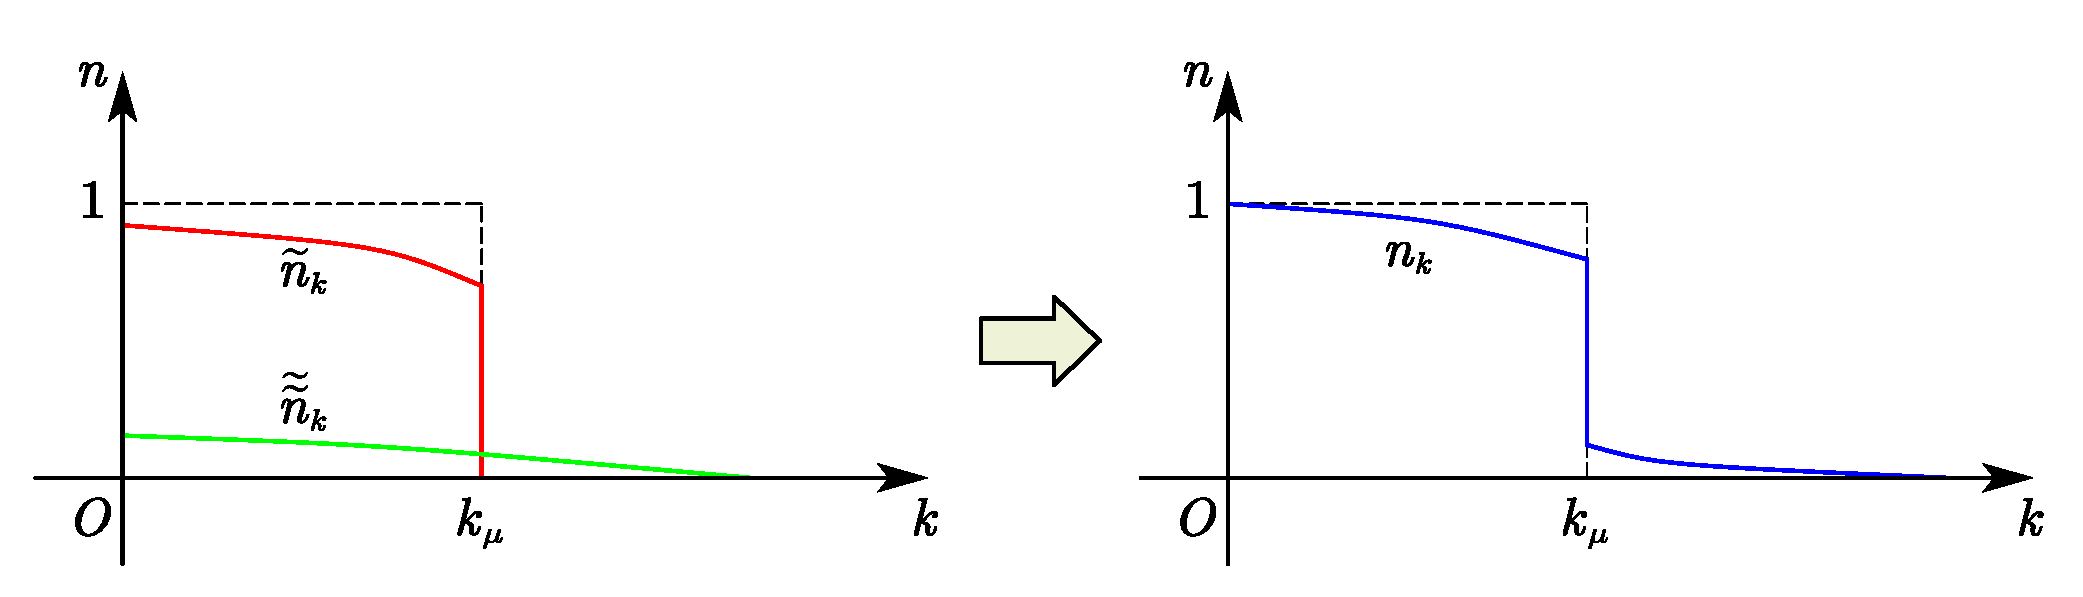
\includegraphics[width=15cm]{figure/dist.pdf}
    \caption{最强发散项近似下的基态电子分布函数示意图.}
    \label{MD-nk}
\end{figure}

凝胶模型的最强发散项近似能够反映系统的等离振荡. 但进一步考虑该模型电子关联, 需要利用密度关联格林函数, 得到介电函数的零点, 即格林函数的极点. 下面利用费曼图对这一方法进行讨论.
\subsection{密度关联格林函数}
回顾前面得到的, 电子间严格的有效相互作用的费曼图是 
\begin{equation}
    \feyndiagram{\propag[doublefermion, dashed] (1,0) to (-1,0);}=
    \feyndiagram{\propag[chasca] (1,0) to (-1,0);}
    +\feyndiagram{
        \normalpolar{a}{0,0};
            \propag[chasca](a) to (-1.5,0);
            \propag[doublefermion, dashed] (1.5,0) to (a);
    },
\end{equation}
对应的表达式: 
\begin{equation}
    \tilde{U}(k)=\frac{U(k)}{1-U(k)\Pi^{*}(k)}=\frac{V(\vct{k})}{1-V(\vct{k})\Pi^{*}(k)},
\end{equation}

严格的总极化图展开式为
\begin{equation}
    \singlepolar=\;
    \singlenormalpolar
    +
    \feyndiagram{
        \normalpolar{a}{-1,0};
        \polar{b}{0.5,0};
        \propag[sca] (a) to (b);
    },
\end{equation}
对应的表达式为 
\begin{equation}
    \Pi(k)=\frac{\Pi^*(k)}{1-U(k)\Pi^*(k)}=\frac{\Pi^*(k)}{1-V(\vct{k})\Pi^*(k)}.
\end{equation}

最强发散项近似的有效相互作用表达式为
\begin{equation}
    \feyndiagram{\propag[doublefermion, dashed] (1,0) to (-1,0);}=
    \feyndiagram{\propag[chasca] (1,0) to (-1,0);}
        +
        \feyndiagram{
            \vertex[ringblob] (a) at (0,0){};
            \propag[chasca](a) to (-1.5,0);
            \propag[doublefermion, dashed] (1.5,0) to (a);
        }.
\end{equation}
对应的数学表达式为 
\begin{equation}
    \tilde{U}_{\fun{MD}}(k)=\frac{U(k)}{1-U(k)\Pi^{*(0)}(k)}=\frac{V(\vct{k})}{1-V(\vct{k})\Pi^{*(0)}(k)}.
\end{equation}
在这一近似下, 极化图展开为
\begin{equation}
    \singlepolar=\;
    \feyndiagram{\vertex[ringblob]at(0,0){};}
    +
    \feyndiagram{
        \vertex[ringblob](a)at(-1,0){};
        \polar{b}{0.5,0};
        \propag[sca] (a) to (b);
    },
\end{equation}
对应的表达式为 
\begin{equation}
    \Pi_{\fun{MD}}(k)=\frac{\Pi^{*(0)}(k)}{1-U(k)\Pi^{*(0)}(k)}=\frac{\Pi^{*(0)}(k)}{1-V(\vct{k})\Pi^{*(0)}(k)}.
\end{equation}
总极化 $\Pi_{\fun{MD}}(k)$ 对应着(因果)密度关联格林函数, $\Pi^{*(0)}$ 是 Lindhard 函数. 这一形式可以得出与上一章相同的结果. 

有效相互作用可以进一步改写成 
\begin{equation}
    \tilde{U}(k)\equiv \frac{U(k)}{\epsilon(k)}=\frac{V(\vct{k})}{\epsilon(k)},
\end{equation}
其中有 
\begin{equation}
    \epsilon(k)=1-V(\vct{k})\Pi^*(k)
\end{equation}
称为系统介电函数. 最强发散项近似下有 
\begin{equation}
    \epsilon_{\fun{MD}}(k)=1-V(\vct{k})\Pi^{*(0)}(k).
\end{equation}
于是有一般成立的关系式:
\begin{equation}
    \frac{1}{\epsilon(k)}=1+V(\vct{k})\Pi(k)\Rightarrow \frac{1}{\epsilon_{\fun{MD}}(k)}=1+V(\vct{k})\Pi_{\fun{MD}}(k).
\end{equation}
下面具体计算在几种极限下的 Lindhard 函数.

(A) 长波极限($q\to 0$).

根据之前的计算, 得到 
  \begin{align}
        \Pi^{*(0)}(\vct{q},\omega)=&2\int\frac{\dd\vct{k}}{(2\pi)^3}\theta(|\vct{k}+\vct{q}|-k_{\fun{F}})\theta(k_{\fun{F}}-|\vct{k}|)\nonumber\\
        &\times \lmi \frac{1}{\omega-\omega_{kq}+\ii\eta}-\frac{1}{\omega+\omega_{kq}-\ii\eta} \rmi,
    \end{align}
其中 
\begin{equation}
    \omega_{kq}\equiv \epsilon_{k+q}^0-\epsilon_k^0=\frac{1}{2m}\ls q^2+2\vct{q}\cdot \vct{k} \rs.
\end{equation}
采用球极坐标
$$
\begin{tikzpicture}
    \draw [arrows = {-Stealth[reversed,reversed]}] (0,0) -- (2,0);
    \draw [arrows = {-Stealth[reversed,reversed]}] (0,0) -- (0,2);
    \draw [arrows = {-Stealth[reversed,reversed]}] (0,0) -- (-1.4,-1);
    \draw [arrows = {-Stealth[harpoon]}] (-0.3,1) -- (-0.3,1.7);
    \draw (-0.6,1.7) node{$\vct{q}$};
    \draw (2.3,0) node{$k_y$};
    \draw (0,2.3) node{$k_z$};% node和文字大括号之间不要加空格.
    \draw (-1.5,-1.4) node{$k_x$};
    \draw (-0.1,-0.3) node{$O$};
    \draw [very thick, arrows = {-Stealth[reversed,reversed]}] (0,0) -- (1,1.4);
    \draw [line width =1pt, dashed] (1,1.4) -- (1,-1.3);
    \draw [line width =1pt, dashed] (1,-1.3) -- (0,0);
    \draw (1.2,1.6) node{$\vct{k}$};
    \draw [-Stealth] (0,1) arc [start angle=90, end angle=40, radius=20pt];
    \draw [-Stealth] (-0.7,-0.5) arc [start angle=-120, end angle=-69, radius=40pt];
    \draw (0.3,1.3) node{$\theta$};
    \draw (0,-1) node{$\varphi$};
\end{tikzpicture}
$$
Lindhard 函数进一步写成 
  \begin{align}
        \Pi^{*(0)}(\vct{q},\omega)=&\frac{2}{(2\pi)^3}\int_0^{2\pi}\dd\varphi\int_0^\pi\sin\theta\dd\theta\int_{|\vct{k}|\le k_{\fun{F}},\atop |\vct{k}+\vct{q}|>k_{\fun{F}}}k^2 \dd k\nonumber\\
        &\times\lmi \frac{1}{\omega-\frac{1}{2m}\ls q^2+2kq\cos\theta \rs+\ii\eta}-\frac{1}{\omega+\frac{1}{2m}(q^2+2kq\cos\theta)-\ii\eta} \rmi,
    \end{align}
在长波极限下, $\vct{q}$ 取值很小, 相应有 $\vct{k}\to \vct{k}_{\fun{F}}$. 取极限 $k\to k_{\fun{F}}$, $q$ 只保留到一次项, $q^2=0$. 于是积分与 $k$ 无关. 利用对 $k$ 的限制:
\begin{itemize}
    \item $k\le k_{\fun{F}}$,
    \item $\sqrt{k^2+q^2+2qk\cos\theta}>k_{\fun{F}}\Rightarrow k+q\cos\theta>k_{\fun{F}}\Rightarrow\cos\theta>0$,
    \item $k>k_{\fun{F}}-q\cos\theta$,
\end{itemize} 
积分式可以写成 
 \begin{align}
        \Pi^{*(0)}(\vct{q},\omega)=&\frac{1}{2\pi^2}\int_0^{\pi/2}\sin\theta\dd\theta \int_{k_{\fun{F}}-q\cos\theta}^{k_{\fun{F}}}k_{\fun{F}}^2\dd k\nonumber\\
        &\times \lmi \frac{1}{\omega-\frac{1}{2m}\ls 2k_{\fun{F}}q\cos\theta \rs+\ii\eta} -\frac{1}{\omega+\frac{1}{2m}(2k_\fun{F}q\cos\theta)-\ii\eta}\rmi,
    \end{align}
令 $x=\cos\theta$, 有 
 \begin{align}
        \Pi^{*(0)}(\vct{q},\omega)=&\frac{q k_{\fun{F}}^2}{2\pi^2}\int_0^1\dd x\; x\nonumber\\
        &\times\lmi \frac{1}{\omega-\frac{k_{\fun{F}}qx}{m}+\ii\eta}-\frac{1}{\omega+\frac{k_{\fun{F}}qx}{m}-\ii\eta} \rmi,
    \end{align}
再引入 $\displaystyle\xi\equiv \frac{m\omega}{k_{\fun{F}}q}$, 得到 
\begin{equation}
    \Pi^{*(0)}(\vct{q},\omega)=\frac{mk_{\fun{F}}}{2\pi^2}\int_0^1 \dd x\; x\lmi \frac{1}{\xi-x+\ii\eta}-\frac{1}{\xi+x-\ii\eta} \rmi.
\end{equation}
利用柯西主值积分, 第一项: 
  \begin{align}
        \int_0^1\dd x\; x\frac{1}{\xi-x+\ii\eta}=&\int_0^1\dd x\; x\lmi \frac{\mathcal{P}}{\xi-x}-\ii\pi\delta(\xi-x) \rmi\nonumber\\
        =&\mathcal{P}\int_0^1\dd x\frac{x-\xi+\xi}{\xi-x}-\ii\pi\xi\theta(1-\xi)\theta(\xi)\nonumber\\
        =&-1-\xi\mathcal{P}\int_0^1\frac{\dd x}{x-\xi}-\ii\pi\xi\theta(1-\xi)\theta(\xi),
    \end{align}
其中, 当 $0<\xi<1$ 时, 有 
\begin{equation}
    \mathcal{P}\int_0^1\frac{\dd x}{x-\xi}=\int_0^{\xi-\delta}\frac{\dd x}{x-\xi}+\int_{\xi+\delta}^1\frac{\dd x}{x-\xi}=\ln \left| \frac{1-\xi}{\xi} \right|.
\end{equation}
代回第一项积分, 有 
\begin{equation}
    \int_0^1\dd x\frac{x}{\xi-x+\ii\eta}=-1-\xi\ln\left| \frac{1-\xi}{\xi} \right|-\ii\pi\xi\theta(1-\xi),\quad (0<\xi<1).
\end{equation}
类似地, 有第二项
 \begin{align}
        -\int_0^1\dd x\frac{x}{\xi+x-\ii\eta}=&-1+\xi\ln\left| \frac{1+\xi}{\xi} \right|+\ii\pi\xi\theta(1+\xi),\quad (-1<\xi<0)\nonumber\\
        =&-1+\xi\ln\left| \frac{1+\xi}{\xi} \right|-\ii\pi|\xi|\theta(1-|\xi|).
    \end{align}
两项合并, 得到 
\begin{equation}
    \int_0^1\dd x\;x\lmi \frac{1}{\xi-x+\ii\eta}-\frac{1}{\xi+x-\ii\eta} \rmi=-2+\xi\ln\left| \frac{1+\xi}{1-\xi} \right|-\ii\pi\theta(1-|\xi|)|\xi|.
\end{equation}
代回 Lindhard 函数中, 有 
\begin{equation}
    \Pi^{*(0)}(\vct{q},\omega)=\frac{-mk_{\fun{F}}}{\pi^2}\lmi 1-\frac{\xi}{2}\ln\left| \frac{1+\xi}{1-\xi} \right|+\frac{\ii\pi}{2}|\xi|\theta(1-|\xi|) \rmi,
\end{equation}
其中有 $\displaystyle \xi\equiv \frac{m\omega}{k_{\fun{F}}q}$, $q\to 0$, $\xi\to \infty$. 考虑小量展开 
\begin{equation}
    \ln\left| \frac{1+\xi}{1-\xi} \right|\approx \frac{2}{\xi}+\frac{2}{3}\frac{1}{\xi^3},
\end{equation}
有 
\begin{equation}
    \Pi^{*(0)}(\vct{q}\to 0,\omega)=\frac{mk_{\fun{F}}}{\pi^2}\frac{1}{3}\ls \frac{k_{\fun{F}}q}{m\omega} \rs^2=\frac{nq^2}{m\omega^2},\quad n=\frac{N}{V}.
\end{equation}
总极化的表达式 
\begin{equation}
    \Pi_{\fun{MD}}(\vct{q},\omega)=\frac{\Pi^{*(0)}(\vct{q},\omega)}{1-V(\vct{q})\Pi^{*(0)}(\vct{q},\omega)},
\end{equation}
等离激元的振荡频率由上式的极点方程给出, 即 
 \begin{align}
        1=&V(\vct{q})\Pi^{*(0)}(\vct{q},\omega),\nonumber\\
        \Rightarrow 1=&\frac{4\pi e^2}{q^2}\frac{nq^2}{m\omega^2},\nonumber\\
        \Rightarrow \omega^2=&\frac{4\pi e^2n}{m}= \omega_p^2,\nonumber\\
        \Rightarrow\omega_p=&\sqrt{\frac{4\pi e^2n}{m}},
    \end{align}
即得等离振荡频率, 也就是系统集体激发的准粒子能谱. 

(B) 静电屏蔽($\omega=0$).

Lindhard 函数: 
 \begin{align}
        \Pi^{*(0)}=&-4\int\frac{\dd\vct{k}}{(2\pi)^3}\frac{\theta(|\vct{k}+\vct{q}|-k_{\fun{F}})\theta(k_{\fun{F}}-|\vct{k}|)}{\epsilon_{k+q}^0-\epsilon_k^0}\nonumber\\
        =&-4\int\frac{\dd \vct{k}}{(2\pi)^3}\frac{[1-\theta(k_{\fun{F}}-|\vct{k}+\vct{q}|)]\theta(k_{\fun{F}}-|\vct{k}|)}{\epsilon_{k+q}^0-\epsilon_k^0},
    \end{align}
其中, 虚部始终为零. 考虑括号中第二项: 
\begin{equation}
        A=4\int\frac{\dd\vct{k}}{(2\pi)^3}\frac{\theta(k_{\fun{F}}-|\vct{k}+\vct{q}|)\theta(k_{\fun{F}}-|\vct{k}|)}{\epsilon_{k+q}^0-\epsilon_k^0},
\end{equation}
作变量代换, 有 $\vct{k}\to -\vct{k}-\vct{q}$, 得到 
\begin{equation}
    A=4\int\frac{\dd\vct k}{(2\pi)^3}\frac{\theta(k_{\fun{F}}-|\vct{k}|)\theta(k_{\fun{F}}-|\vct{k}+\vct{q}|)}{\epsilon_k^0-\epsilon_{k+q}^0},
\end{equation}
这里得到的结果, 分子不变, 分母差一负号, 即有 $A=-A\Rightarrow A=0$. 于是 $\Pi^{*(0)}$ 表达式中只需要考虑第一项. 有:
\begin{align}
        \Pi^{*(0)}(\vct{q},0)=&-4\int\frac{\dd \vct{k}}{(2\pi)^3}\frac{\theta(k_{\fun{F}}-|\vct{k}|)}{\frac{1}{2m}(q^2+2\vct{q}\cdot \vct{k})}\nonumber\\
        =&-\frac{2m}{\pi^2}\int_0^{k_{\fun{F}}}k^2\dd k\int_{-1}^1\frac{\dd x}{q^2+2qkx}\nonumber\\
        =&-\frac{m}{\pi^2 q}\int_0^{k_{\fun{F}}}k\dd k\ln\left| \frac{q^2+2qk}{q^2-2qk} \right|,
    \end{align}
其中第二步取 $x\equiv \cos\theta$. 再利用积分公式 
\begin{equation}
    \int\dd x x\ln|x+a|=\frac{1}{2}(x^2-a^2)\ln|x+a|-\frac{x^2}{4}+\frac{ax}{2},
\end{equation}
表达式进一步写成 
\begin{equation}
    \Pi^{*(0)}(\vct{q},0)=-\frac{mk_{\fun{F}}}{2\pi^2}\lmi 1+\frac{1}{y}\ls 1-\frac{y^2}{4} \rs\ln\left| \frac{1+\frac{y}{2}}{1-\frac{y}{2}} \right| \rmi,
\end{equation}
其中有 $y\equiv q/k_{\fun{F}}$. 下面利用这一结果来讨论系统的有效相互作用.
 \begin{align}
        \tilde U_{\fun{MD}}(\vct{q},0)=&\frac{V(\vct{q})}{1-V(\vct{q})\Pi^{*(0)}(\vct{q},0)}\nonumber\\
        =&\frac{V(\vct{q})}{\epsilon_{\fun{MD}}(\vct{q},0)}\nonumber\\
        =&\frac{4\pi e^2}{q^2-4\pi e^2\Pi^{*(0)}(\vct{q},0)},
    \end{align}
傅里叶变换到实空间下, 有 
\begin{equation}
    \tilde U_{\fun{MD}}(\vct{r})=\int\frac{\dd\vct{q}}{(2\pi)^3}\tilde U_{\fun{MD}}(\vct{q},0)\e^{\ii\vct{q}\cdot \vct{r}}\propto \frac{\cos(2k_{\fun{F}}r)}{r^3},
\end{equation}
在 $r\to \infty$ 时振荡衰减. 这一结果常称为 Friedel 震荡, 如图\ref{friedel}所示. 

\begin{figure}[htbp]
    \centering
    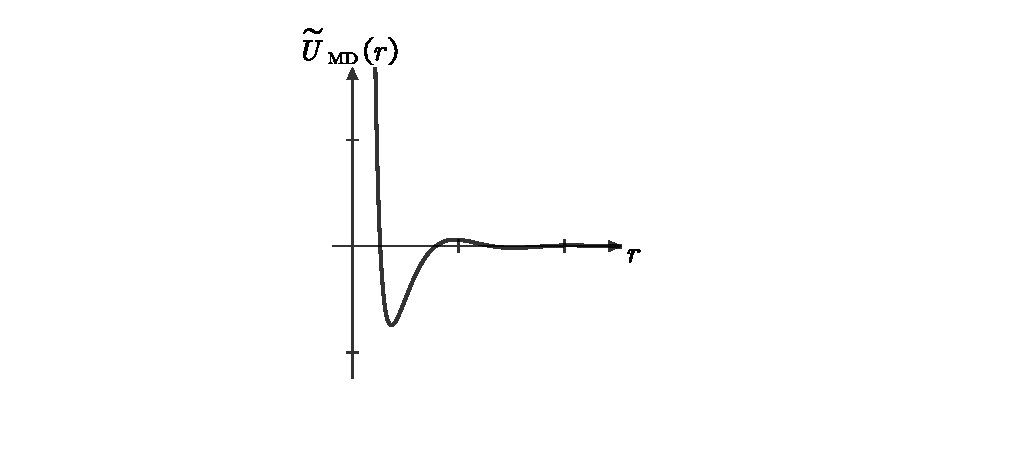
\includegraphics[width=4cm]{figure/friedel.pdf}
    \caption{Friedel 震荡函数.}
    \label{friedel}
\end{figure}

下面讨论 $q\to 0,\omega\to 0$ 的情况: 
\begin{equation}
    \Pi^{*(0)}(\vct{q}\to 0,0)=-\frac{mk_{\fun{F}}}{\pi^2},
\end{equation}
\begin{equation}
    \tilde U_{\fun{MD}}(\vct q\to 0,0)=\frac{4\pi e^2}{q^2+4\pi e^2\frac{mk_{\fun{F}}}{\pi^2}}=\frac{4\pi e^2}{q^2+\lambda^2},
\end{equation}
其中有 
\begin{equation}
    \lambda^2\equiv \frac{4 e^2mk_{\fun{F}}}{\pi}=\frac{6\pi ne^2}{E_{\fun{F}}},\quad n=\frac{N}{V},
\end{equation}
我们称 
\begin{equation}
    \lambda^{-1}=\frac{1}{\sqrt{\frac{6\pi ne^2}{E_{\fun{F}}}}}
\end{equation}
为 Thomas-Fermi 屏蔽长度. 并有 
\begin{equation}
    \tilde{U}_{\fun{MD}}(\vct{r})=\frac{e^2}{r}\e^{-\lambda r}
\end{equation}
称为汤川(Yukawa)屏蔽势, 如图\ref{yukawa}所示.
\begin{figure}[htbp]
    \centering
    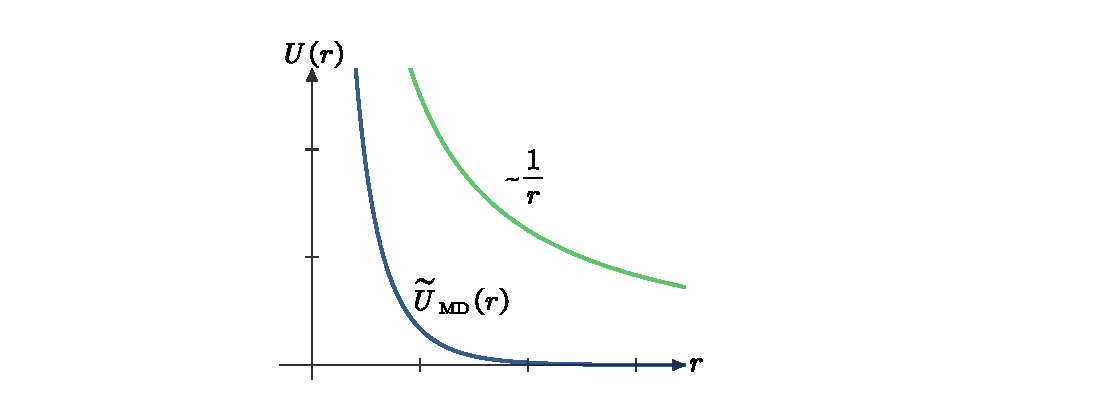
\includegraphics[width=5cm]{figure/yukawa.pdf}
    \caption{汤川屏蔽势和库仑势.}
    \label{yukawa}
\end{figure}
\begin{note}
    下面讨论一下最强发散项近似的成立条件.

    考虑这样三种自能图:
    $$
        \feyndiagram{
            \vertex(a)at(-1,-1);
            \vertex(b)at(1,-1);
            \vertex(c)at(-1,1);
            \vertex(d)at(1,1);
            \propag[plain](a)to(b);
            \propag[sca](a)to(c);
            \propag[sca](b)to(d);
            \propag[plain](c)to[half left, looseness=1.5](d);
            \propag[plain](d)to[half left, looseness=1.5](c);
            \vertex(e)at(-1.3,0){$\vct{q}$};
            \vertex(f)at(1.3,0){$\vct{q}$};
        },\quad
        \feyndiagram{
            \vertex(a)at(-1,-1);
            \vertex(b)at(1,-1);
            \vertex(c)at(-1,1);
            \vertex(d)at(1,1);
            \propag[plain](a)to(b);
            \propag[sca](a)to(c);
            \propag[sca](b)to(d);
            \propag[plain](c)to[half left, looseness=1.5](d);
            \propag[plain](d)to[half left, looseness=1.5](c);
            \vertex(e)at(-1.3,0){$\vct{q}$};
            \vertex(f)at(1.3,0){$\vct{q}$};
            \propag[sca](0,1.8)to(0,0.1);
        },\quad
        \feyndiagram{
            \vertex(a)at(-1,-1);
            \vertex(b)at(1,-1);
            \vertex(c)at(-1,1);
            \vertex(d)at(1,1);
            \propag[plain](a)to(b);
            \propag[sca](a)to(c);
            \propag[sca](b)to(d);
            \propag[plain](c)to[half left, looseness=1.5](d);
            \propag[plain](d)to[half left, looseness=1.5](c);
            \vertex(e)at(-1.3,0){$\vct{q}$};
            \vertex(f)at(1.3,0){$\vct{q}$};
            \propag[sca](-0.4,1.7)to(-0.4,0.3);
            \propag[sca](0.4,1.7)to(0.4,0.3);
        },\quad
    $$
    这三种图的发散程度相同, 但我们在取近似时, 只考虑了第一种, 而忽略了后两种. 这是因为在高密度情况下, 第一项的贡献要远大于其它项. 下面证明这一结论.

    在高密度近似下, 假设一个电子所占据的体积可以用等体积的球来描述, 即有 
    \begin{equation}
        \frac{V}{N}\equiv \frac{4}{3}\pi r^3_0.
    \end{equation}
    引入无量纲参数 $r_s$, 令 $r_0\equiv r_sa_H$, 其中 $a_H$ 是氢原子玻尔第一轨道半径, 有 $a_H=\hbar^2/me^2$.
    高密度近似对应着 $r_s\ll 1$, 即 
    \begin{equation}
        r_s=\frac{\ls \frac{9}{4}\pi \rs^{1/3}}{a_Hk_{\fun{F}}}\ll 1\Rightarrow \frac{1}{a_Hk_{\fun{F}}}\ll 1.
    \end{equation}
    下面主要分析 $\feyndiagram{\vertex[ringblob](0,0){};}$ 和 $\feyndiagram{\propag[plain](-0.4,0)to[half left, looseness=1.8](0.4,0);\propag[plain](0.4,0)to[half left, looseness=1.8](-0.4,0);\propag[sca](0,-0.4)to(0,0.4);}$ 的贡献.

    (a)
    $$
    \feyndiagram{
        \vertex(c)at(-1,0);
        \vertex(d)at(1,0);
        \propag[fer](c)to[half left, looseness=1.5](d);
        \propag[fer](d)to[half left, looseness=1.5](c);
        \vertex(a)at(0,-1.3){$\vct{k}+\vct{k}_1$};
        \vertex(v)at(0,1.3){$\vct{k}_1$};
    }
    $$
    \begin{equation}
        \Pi^{*(0)}(k)=-2\ii\int\frac{\dd k_1}{(2\pi)^4}G^0(k+k_1)G^0(k_1).
    \end{equation}

    (b)
    $$
    \feyndiagram{
        \vertex(a)at(-1,0);
        \vertex(b)at(1,0);
        \vertex(c)at(0,1);
        \vertex(d)at(0,-1);
        \propag[fer](a)to[quarter left, looseness=1](c);
        \propag[fer](c)to[quarter left, looseness=1](b);
        \propag[fer](b)to[quarter left, looseness=1](d);
        \propag[fer](d)to[quarter left, looseness=1](a);
        \propag[sca](c)to(d);
        \vertex (1) at (-1,-1.2){$\vct{k}_2+\vct{k}$};
        \vertex (2) at (-1,1.2){$\vct{k}_2$};
        \vertex (3) at (1,1.2){$\vct{k}_1$};
        \vertex (4) at (1,-1.2){$\vct{k}_1+\vct{k}$};
        \vertex (5) at (-0.2,0){$\vct{k}_2-\vct{k}_1$};
    }
    $$
      \begin{align}
            \Pi^{*(1)}(k)=&-2\ii^2\int\frac{\dd k_1}{(2\pi)^4}\int\frac{\dd k_2}{(2\pi)^4}G^0(k_1+k)G^0(k_1) V(\vct{k}_1-\vct{k}_2)G^0(k_2+k)G^0(k_2)\nonumber\\
            =&-2\ii^2\frac{4\pi e^2}{k_{\fun{F}}^2}\lmi \int\frac{\dd k_1}{(2\pi)^4}G^0(k_1+k)G^0(k_1) \rmi\lmi \int\frac{\dd k_2}{(2\pi)^4}G^0(k_2+k)G^0(k_2) \rmi,
        \end{align}
    可以看出, 两个表达式的关系为 
    \begin{equation}
        \left| \Pi^{*(1)}(k) \right|\sim\frac{e^2}{k_{\fun{F}}^2}\left| \Pi^{*(0)}(k) \right|^2,
    \end{equation}
    考虑两个函数的比值, 有 
    \begin{equation}
        \frac{\left| \Pi^{*(1)}(k) \right|}{\left| \Pi^{*(0)}(k) \right|}\sim\frac{e^2}{k_{\fun{F}}^2}\left| \Pi^{*(0)}(k) \right|\sim\frac{e^2}{k_{\fun{F}}^2}mk_{\fun{F}}=\frac{me^2}{k_{\fun{F}}}\sim\frac{1}{k_{\fun{F}}a_H}.
    \end{equation}
    上式在高密度极限下远小于 1. 于是有 $|\Pi^{*(1)}(k)|\ll |\Pi^{*(0)}(k)|$ 可以忽略, 对应着电子的无规则相位最强. 这是近似成立的条件.
\end{note}
\begin{question}{}{}
    计算下面两个动量空间费曼图, 要求对所有内部自旋求和, 所有内部频率积分.
    $$
        \feyndiagram{
            \propag[plain](-2,0) to (2,0);
            \propag[plain](-1,1.5) to[half left, looseness=1.5](1,1.5);
            \propag[plain](1,1.5) to[half left, looseness=1.5](-1,1.5);
            \propag[sca](0,0)to(0,0.6);
            \propag[sca](-1,0) to (-1,1.5);
            \propag[sca](1,0)to(1,1.5);
        }
        \qquad
        \feyndiagram{
            \propag[plain](-2,0) to (2,0);
            \propag[sca](-1.5,0)to[half left, looseness=1.6](0.5,0);
            \propag[sca](-0.5,0) to[half left, looseness=1.6](1.5,0);
        }
    $$
\end{question}
\setcounter{chapter}{3}
\chapter{有限温单粒子格林函数, 费曼图技术及其应用}
\begin{introduction}
\item 松原(Matsubara)格林函数
\item 物理量的表示
\item 松原格林函数的若干性质及傅里叶变换
\item 自由粒子的松原格林函数
\item 松原格林函数的 Lehmann 表示
\item 其他单粒子热力学格林函数(实时)
\item 相互作用绘景下的松原格林函数
\item Wick 定理
\item 松原格林函数的坐标空间费曼图规则
\item 松原格林函数的动量空间费曼图规则
\item 松原格林函数的频率求和方法
\item 松原格林函数的应用
\end{introduction}
目前为止我们讲到的三种格林函数都是零温情况的, 它们分别是因果格林函数, 推迟格林函数和超前格林函数. 其中, 因果格林函数可以利用 Wick 定理展开. 

现在要讨论的是有限温度下的系统. 可以引入有限温度下的因果、推迟和超前热力学格林函数, 但不能直接由零温格林函数通过代换基态平均得到. 此时必须考虑另外一种格林函数. 日本京都大学的松原教授提出一个非常巧妙的方案, 人们称为松原格林函数, 也称为虚时格林函数. 在有限温度中, 只有这种格林函数可以利用费曼图技术, 其他格林函数可以利用相互之间的关系式求出来. 下面介绍松原格林函数.
\section{松原(Matsubara)格林函数}
考虑有限温度时, 采用巨正则系综比较方便. 

巨正则系综下, 哈密顿量改写为: $\hat{H}\to \hat{H}-\mu\hat{N}\equiv \hat{K}$, 其中 $\mu$ 是系统的化学势, $\hat{N}$ 是总粒子数算符.

有限温情况下, 需要引入密度算符处理混合态: 
\begin{equation}
    \hat{\rho}\equiv \frac{\e^{-\beta\hat{K}}}{\Xi },
\end{equation}
其中 $\beta=1/k_{\fun{B}}T$, $\Xi$ 是巨正则系综的配分函数, 表达式为 
\begin{equation}
    \Xi=\fun{Tr}\lmi \e^{-\beta \hat{K}} \rmi.
\end{equation}
巨正则系综下, 有类似于正则系综中自由能的热力学势 
\begin{equation}
    \Omega\equiv -\frac{1}{\beta}\ln \Xi,
\end{equation}
配分函数可以用热力学势表示为 
\begin{equation}
    \Xi =\e^{-\beta\Omega},
\end{equation}
相应的可以把密度算符表示成 
\begin{equation}
    \hat{\rho}=\e^{\beta (\Omega-\hat{K})}.
\end{equation}
巨正则系综中, 算符的平均值可以用密度算符表示为 
\begin{equation}
    \lag \hat{A} \rag_T=\fun{Tr}\lmi \e^{\beta(\Omega-\hat{K})}\hat{A} \rmi,
\end{equation}
通常通过粒子数算符的平均值来确定化学势 $\mu$, 有 
\begin{equation}
    \lag \hat{N} \rag_T=\fun{Tr}\lmi \e^{\beta(\Omega-\hat{K}) }\hat{N} \rmi_\mu=N.
\end{equation}

设 $\hat{H}$ 不显含时间, 巨正则系综的场算符在诸绘景下可以表示为:
\begin{itemize}
    \item 薛定谔绘景: 
    \begin{equation}
        \hat{\psi}^{}_{\alpha}(\vct{x}),\quad \hat{\psi}_\beta^\dg (\vct{x}'). 
    \end{equation}
    \item 海森伯绘景: 
    \begin{equation}
        \hat{\psi}_{H\alpha}^{ }(\vct{x},\tau)\equiv \e^{\hat{K}\tau}\hat{\psi}_\alpha(\vct{x})\e^{-\hat{K}\tau},\quad \hat{\psi}^\dg_{H\alpha}(\vct{x},\tau)\equiv \e^{\hat{K}\tau}\hat{\psi}_\alpha^\dg (\vct{x})\e^{-\hat{K}\tau}.
    \end{equation}
    与零温情况相比, $\tau\to \ii t$ 称为虚时, 取值范围 $\tau \in [0,\beta]$. 此处需要注意的是, 虚时情况的海森伯绘景场算符并不是厄米算符, 即 
    \begin{equation}
        \hat{\psi}_{H\alpha} (\vct{x},\tau)\ne \lmi \hat{\psi}^{}_{H\alpha}(\vct{x},\tau) \rmi^\dg.
    \end{equation}
\end{itemize}
有限温格林函数将采用海森伯绘景下的虚时场算符. 下面给出松原格林函数的定义.

\begin{definition}{松原格林函数}{}
  \begin{align}
        \mathcal{G}_{\alpha\beta}(\vct{x},\tau; \vct{x}',\tau')\equiv& -\fun{Tr}\lmi \hat{\rho}\hat{T}^{}_\tau \left[\hat{\psi}^{ }_{H\alpha}(\vct{x},\tau)\hat{\psi}^\dg_{H\beta}(\vct{x}',\tau')\right] \rmi\nonumber\\
        =&-\llag \hat{T}^{}_\tau \lmi \hat{\psi}_{H\alpha}^{ }(\vct{x},\tau)\hat{\psi}_{H\beta}^\dg (\vct{x}',\tau') \rmi \rrag_T.
    \end{align}
\end{definition}
\section{物理量的表示}
\subsection{单体算符的平均值}
单体算符的一般表达式为 
\begin{equation}
    F_2^{(1)}=\sum_\alpha\sum_\beta\int\hat{\psi}_\alpha^\dg (\vct{x})\hat{f}_{\alpha\beta}(\vct{x})\hat{\psi}_\beta^{ }(\vct{x})\dd \vct{x},
\end{equation}
单体算符在有限温下的平均值表示为 
    \begin{align}
        \llag \hat{F}_2^{(1)} \rrag_T=&\sum_\alpha\sum_\beta\int\dd \vct{x}\fun{Tr}\lmi \hat{\rho}\hat{\psi}_\alpha^\dg (\vct{x})\hat{f}_{\alpha\beta}(\vct{x})\hat{\psi}_\beta^{ }(\vct{x}) \rmi\nonumber\\
        =&\sum_\alpha\sum_\beta\int\dd \vct{x}\lim_{\vct{x}'\to \vct{x}}\hat{f}^{}_{\alpha\beta}(\vct{x})\fun{Tr}\lmi \hat{\rho}\hat{\psi}_\alpha^\dg(\vct{x}')\hat{\psi}_\beta^{ }(\vct{x}) \rmi\nonumber\\
        =&\sum_\alpha\sum_\beta\int\dd \vct{x}\lim_{\vct{x}'\to \vct{x}}\hat{f}^{}_{\alpha\beta}(\vct{x})\fun{Tr}\lmi \hat{\rho}\e^{-\hat{K}\tau}\hat{\psi}_{H\alpha}^\dg (\vct{x}',\tau)\e^{\hat{K}\tau} \e^{-\hat{K}\tau}\hat{\psi}_{H\beta}^{ }(\vct{x},\tau)\e^{\hat{K}\tau} \rmi\nonumber\\
        =&\sum_\alpha\sum_\beta\int\dd \vct{x}\lim_{\vct{x}'\to \vct{x}\atop \tau'\to \tau^+}\hat{f}^{}_{\alpha\beta}(\vct{x})\fun{Tr}\lmi \hat{\rho}\hat{\psi}_{H\alpha}^\dg (\vct{x}',\tau')\hat{\psi}_{H\beta}^{ }(\vct{x},\tau) \rmi\nonumber\\
        =&\sum_\alpha\sum_\beta\int\dd \vct{x}\lim_{\vct{x}'\to \vct{x}\atop \tau'\to \tau^+}\hat{f}^{}_{\alpha\beta}(\vct{x})\fun{Tr}\lmi \hat{\rho}\hat{T}_{\tau}\left[\hat{\psi}_{H\alpha}^\dg (\vct{x}',\tau')\hat{\psi}_{H\beta}^{ }(\vct{x},\tau)\right] \rmi\nonumber\\
        =&\pm\sum_\alpha\sum_\beta\int\dd \vct{x}\lim_{\vct{x}'\to \vct{x}\atop \tau'\to \tau^+}\hat{f}^{}_{\alpha\beta}(\vct{x})\fun{Tr}\lmi \hat{\rho}\hat{T}_{\tau}\left[\hat{\psi}_{H\beta}^{ }(\vct{x},\tau)\hat{\psi}_{H\alpha}^\dg (\vct{x}',\tau')\right] \rmi\nonumber\\
        =&\mp\sum_\alpha\sum_\beta\int\dd \vct{x}\lim_{\vct{x}'\to \vct{x}\atop \tau'\to \tau^+}\hat{f}^{}_{\alpha\beta}(\vct{x}) \mathcal{G}_{\beta\alpha}(\vct{x},\tau; \vct{x}',\tau').
    \end{align}
若 $\hat{f}_{\alpha\beta}$ 与自旋无关, 即
\begin{equation}
\hat{f}_{\alpha\beta}=\hat{f}\delta_{\alpha\beta},
\end{equation}
则有
\begin{equation}
 \llag \hat{F}_2^{(1)} \rrag_T=\mp\sum_\alpha\int\dd \vct{x}\lim_{\vct{x}'\to \vct{x}\atop \tau'\to \tau^+}\hat{f}(\vct{x}) \mathcal{G}_{\alpha\alpha}(\vct{x},\tau; \vct{x}',\tau').
\end{equation}

\begin{example}总动量算符

\begin{equation}
\langle\hat{T}\rangle_T=\mp\sum_\alpha\int\dd \vct{x}\lim_{\vct{x}'\to \vct{x}\atop \tau'\to \tau^+}\left(-\frac{\nabla_x^2}{2m}\right) \mathcal{G}_{\alpha\alpha}(\vct{x},\tau; \vct{x}',\tau').
\end{equation}
\end{example}

\begin{example}总粒子数算符

\begin{equation}
\langle\hat{N}\rangle_T=\mp\sum_\alpha\int\dd \vct{x}\lim_{\vct{x}'\to \vct{x}\atop \tau'\to \tau^+} \mathcal{G}_{\alpha\alpha}(\vct{x},\tau; \vct{x}',\tau').
\end{equation}
\end{example}

\begin{example}总自旋算符

\begin{equation}
\langle \hat{S} \rangle_T=\mp\sum_\alpha\sum_\beta\int\dd \vct{x}\lim_{\tau'\to \tau^+}S_{\alpha\beta}\mathcal{G}_{\beta\alpha}(\vct{x},\tau; \vct{x},\tau').
\end{equation}
\end{example}

\subsection{两体相互作用}
两体相互作用可以写作
\begin{equation}
\hat{V}=\frac{1}{2}\sum_{\alpha}\sum_\beta\iint\mathrm{d}\vct x \mathrm{d} \vct x' \hat{\psi}_{\alpha}^{\dg}(\vct x) \hat{\psi}_{\beta}^{\dg}(\vct x')\hat{V}(\vct x-\vct x')\hat{\psi}_{\beta}^{}(\vct x')\hat{\psi}_{\alpha}^{}(\vct x),
\end{equation}
考虑两体相互作用与自旋无关, 则两体相互作用的平均值为
\begin{equation}
\langle\hat{V}\rangle_T=\mp \frac{1}{2} \sum_\alpha \int \mathrm{d} \vct{x} \lim _{\substack{\vct{x}^{\prime} \rightarrow \vct{x} \\ \tau^{\prime} \rightarrow \tau^{+}}}\left[-\frac{\partial}{\partial \tau}+\frac{\nabla_{\vct x}^2}{2 m}+\mu\right] \mathcal{G}_{\alpha \alpha}\left(\vct{x}, \tau ; \vct{x}^{\prime}, \tau^{\prime}\right) .
\end{equation}

\subsection{内能}
内能可以表示为体系哈密顿量的热力学平均, 即
\begin{align}
E=&\langle\hat{H}\rangle_T=\langle\hat{T}\rangle_T+\langle\hat{V}\rangle_T\nonumber\\
=&\mp \frac{1}{2} \sum_\alpha \int \mathrm{d} \vct{x} \lim _{\substack{\vct{x}^{\prime} \rightarrow \vct{x}\\ \tau^{\prime} \rightarrow \tau^{+}}}\left[-\frac{\partial}{\partial \tau}-\frac{\nabla_{\vct x}^2}{2 m}+\mu\right] \mathcal{G}_{\alpha \alpha}\left(\vct{x}, \tau ; \vct{x}^{\prime}, \tau^{\prime}\right) .
\end{align}

\subsection{热力学势 $\Omega$ 的计算公式}
巨正则系综下, 热力学势 $\Omega$ 是一个很重要的物理量. 如果可以计算出体系的热力学势, 就可以得到体系的很多信息. 仿照上一章计算零温基态能的第二种方式, 引入如下赝哈密顿量:
\begin{equation}
\hat{H}(\lambda)=\hat{H}_0+\lambda \hat{H}_1,
\end{equation}
其中 $\lambda \in[0,1]$. $\hat{H}_0$ 表示自由粒子体系的哈密顿量, 通常是总动能 $\hat{T}$. $\hat{H}_1$ 表示粒子间的相互作用, 通常考虑两体相互作用 $\hat{V}$. $\lambda=0$ 时, $\hat{H}(0)$ 表示不考虑相互作用的自由粒子体系的哈密顿量; $\lambda=1$ 时, $\hat{H}(1)$ 是相互作用体系真实的哈密顿量; $(0,1)$ 区间内的 $\lambda$ 对应的哈密顿量 $\hat{H}(\lambda)$, 只是为了方便数学计算, 并不对应实际的哈密顿量. 对于巨正则系综, 还可以引入:
\begin{equation}
\hat{K}(\lambda)=\hat{H}(\lambda)-\mu \hat{N}=\hat{H}_0-\mu \hat{N}+\lambda \hat{H}_1\equiv\hat{K}_0+\lambda \hat{K}_1,
\end{equation}
其中
\begin{equation}
\hat{K}_0 \equiv \hat{H}_0-\mu \hat{N}, \quad \hat{K}_1 \equiv \hat{H}_1.
\end{equation}
按巨配分函数的定义, 可以得到 $\hat{K}(\lambda)$ 对应的巨配分函数:
\begin{equation}
\Xi(\lambda)=\operatorname{Tr}\left[\e^{-\beta \hat{K}(\lambda)}\right],
\end{equation}
则赝哈密顿量 $\hat{H}(\lambda)$ 对应的热力学势为:
\begin{equation}
\Omega(\lambda)=-\frac{1}{\beta} \ln \Xi(\lambda) .
\end{equation}
如果我们计算出松原格林函数表示巨配分函数 $\Xi(\lambda)$ 的形式, 很快就可以得到用松原格林函数表示热力学势 $\Omega(\lambda)$ 的表达式, 但是 $\Xi(\lambda)$ 的松原格林函数表示形式并不容易得到. 按之前计算基态能的方法, 在上式两边对 $\lambda$ 求偏导, 得到:
\begin{equation}
\frac{\partial \Omega(\lambda)}{\partial \lambda}=-\frac{1}{\beta} \frac{1}{\Xi(\lambda)} \frac{\partial \Xi(\lambda)}{\partial \lambda},
\end{equation}
这样上式两边再对 $\lambda$ 从 0 到 1 积分就可以得到相互作用体系的热力学势 $\Omega=\Omega(1)$ 的表达式, 这似乎还是需要计算 $\Xi(\lambda)$, 而且还要计算 $\displaystyle\frac{\partial \Xi(\lambda)}{\partial \lambda}$ . 但在实际计算过程中, $\Xi(\lambda)$ 会被消去, 只需要计算 $\displaystyle\frac{\partial \Xi(\lambda)}{\partial \lambda}$. 下面就来计算这一项:
\begin{align}
\frac{\partial \Xi(\lambda)}{\partial \lambda} =&\frac{\partial}{\partial \lambda} \operatorname{Tr}\left[\sum_{n=0}^{\infty} \frac{[-\beta \hat{K}(\lambda)]^n}{n !}\right]\nonumber \\
=&\sum_{n=0}^{\infty} \frac{(-\beta)^n}{n !} \operatorname{Tr}\left[\frac{\partial}{\partial \lambda}\left(\hat{K}_0+\lambda \hat{K}_1\right)^n\right] \nonumber\\
=&\sum_{n=1}^{\infty} \frac{(-\beta)^n}{n !} \operatorname{Tr}\left[n\left(\hat{K}_0+\lambda \hat{K}_1\right)^{(n-1)}\hat{K}_1\right]\nonumber\\
=&(-\beta) \sum_{n=1}^{\infty} \frac{(-\beta)^{(n-1)}}{(n-1) !} \operatorname{Tr}\left[\left(\hat{K}_0+\lambda \hat{K}_1\right)^{(n-1)} \hat{K}_1\right]\nonumber \\
\stackrel{m=n-1}{\longrightarrow} &(-\beta) \sum_{m=0}^{\infty} \frac{(-\beta)^m}{m !} \operatorname{Tr}\left[\left(\hat{K}_0+\lambda \hat{K}_1\right)^m \hat{K}_1\right]\nonumber \\
=&(-\beta) \operatorname{Tr}\left[\e^{-\beta \hat{K}(\lambda)} \hat{K}_1\right] \nonumber\\
=&-\frac{\beta}{\lambda} \e^{-\beta \Omega(\lambda)} \operatorname{Tr}\left[\e^{\beta(\Omega(\lambda)-\hat{K}(\lambda))} \lambda \hat{K}_1\right] \nonumber\\
=&-\frac{\beta}{\lambda} \e^{-\beta \Omega(\lambda)}\left\langle\lambda \hat{K}_1\right\rangle_\lambda,
\end{align}
这里利用了密度矩阵的表达式，最后的均值与 $\lambda$ 有关，而且是将 $\lambda \hat{K}_1$ 看成一个整体的相互作用进行计算, 所以 $\lambda$ 不能提出来消去. 故:
\begin{equation}
\frac{\partial \Omega(\lambda)}{\partial \lambda}=-\frac{1}{\beta}\frac{1}{\Xi(\lambda)}\left[-\frac{\beta}{\lambda} \e^{-\beta \Omega(\lambda)}\left\langle\lambda \hat{K}_1\right\rangle_\lambda\right]=\frac{\left\langle\lambda \hat{K}_1\right\rangle_\lambda}{\lambda},
\end{equation}
其中利用了热力学势与巨配分函数的关系式. 这样两边对 $\lambda$ 积分得到:
\begin{equation}
\left.\Omega(\lambda)\right|_0 ^1=\int_0^1 \mathrm{~d} \lambda \frac{\left\langle\lambda \hat{K}_1\right\rangle_\lambda}{\lambda}
\end{equation}
最终得到:
\begin{equation}
\Omega=\Omega_0+\int_0^1 \mathrm{~d} \lambda \frac{\left\langle\lambda \hat{K}_1\right\rangle_\lambda}{\lambda},
\end{equation}
其中 $\Omega_0$ 是自由粒子体系的热力学势. 考虑两体相互作用, 即 $\hat{K}_1=\hat{H}_1=\hat{V}$, 参考利用松原格林函数表示 $\hat{V}$ 的表达式, 可以得到完全类似的 $\lambda \hat{K}_1$ 的表达式 (将整个 $\lambda \hat{K}_1$ 看成 $\hat{V}$, 此时的松原格林函数将与 $\lambda$ 有关). 这样可以得到用松原格林函数表示热力学势的最终表达式:
\begin{equation}
\Omega=\Omega_0 \mp \frac{1}{2}\sum_\alpha\int_0^1 \frac{\mathrm{d} \lambda}{\lambda}   \int \mathrm{d} \vct{x} \lim _{\substack{\vct{x}^{\prime} \rightarrow \vct{x} \\ \tau^{\prime} \rightarrow \tau^{+}}}\left[-\frac{\partial}{\partial \tau}+\frac{\nabla_{\vct x}^2}{2 m}+\mu\right] \mathcal{G}\left(\vct{x}, \tau ; \vct{x}^{\prime}, \tau^{\prime} ; \lambda\right) .
\end{equation}

有了热力学势, 就可以得到诸多物理量:
\begin{align}
\langle \hat N \rangle_T &= -\left(\frac{\partial \Omega}{\partial \mu}\right)_{T,V};\\
P &= -\left(\frac{\partial \Omega}{\partial V}\right)_{\mu ,T};\\
S &= -\left(\frac{\partial \Omega}{\partial T}\right)_{\mu ,V}.
\end{align}

\section{松原格林函数的若干性质及傅里叶变换}
\subsection{松原格林函数的对称性}
与零温单粒子格林函数相同, 当体系(或哈密顿量)具有某种对称性, 相应的松原格林函数可以进行简化:
\begin{itemize}
\item 若 $\hat{H}$ 不显含时间, 则 
\begin{equation}
\mathcal{G}_{\alpha \beta}\left(\vct{x}, \tau ; \vct{x}^{\prime}, \tau^{\prime}\right)=\mathcal{G}_{\alpha \beta}\left(\vct{x}, \vct{x}^{\prime} ; \tau-\tau^{\prime}\right);
\end{equation}\\
\item 若体系是空间均匀的, 即 $[\hat{H}, \hat{\vct{P}}]_{-}=0$, 其中$\hat{\vct{P}}$是总动量算符, 则
\begin{equation}
\mathcal{G}_{\alpha \beta}\left(\vct{x}, \tau ; \vct{x}^{\prime}, \tau^{\prime}\right)=\mathcal{G}_{\alpha \beta}\left(\vct{x}-\vct{x}^{\prime} ; \tau, \tau^{\prime}\right);
\end{equation}\\
\item 若相互作用与自旋无关, 则 
\begin{equation}
\mathcal{G}_{\alpha \beta}\left(\vct{x}, \tau ; \vct{x}^{\prime}, \tau^{\prime}\right)=\delta_{\alpha \beta} \mathcal{G}\left(\vct{x}, \tau ; \vct{x}^{\prime}, \tau^{\prime}\right),
\end{equation}
其中 
\begin{equation}
\mathcal{G}\left(\vct{x}, \tau ; \vct{x}^{\prime}, \tau^{\prime}\right)=\frac{\sum\limits_{ \alpha} \mathcal{G}_{\alpha \alpha}\left(\vct{x}, \tau ; \vct{x}^{\prime}, \tau^{\prime}\right)}{2 S+1}.
\end{equation} 
\end{itemize}
\subsection{松原格林函数的周期性与反周期性}
考虑体系的哈密顿量不显含时间, 即 
\begin{equation}
\mathcal{G}_{\alpha \beta}\left(\vct{x}, \tau ; \vct{x}^{\prime}, \tau^{\prime}\right)=\mathcal{G}_{\alpha \beta}\left(\vct{x}, \vct{x}^{\prime} ; \tau-\tau^{\prime}\right)\equiv\mathcal{G}_{\alpha \beta}\left(\vct{x}, \vct{x}^{\prime} ; \tilde{\tau}\right).
\end{equation} 
这里定义了 $ \tilde{\tau}\equiv\tau-\tau^{\prime}$, 由 $\tau, \tau^{\prime} \in[0, \beta]$ 可知 $\tilde{\tau} \in[-\beta, \beta]$. 这时可以得出松原格林函数有如下周期性(反周期性):
\begin{equation}
\mathcal{G}_{\alpha \beta}\left(\vct{x}, \vct{x}^{\prime} ; \tilde{\tau}<0\right)=\pm \mathcal{G}_{\alpha \beta}\left(\vct{x}, \vct{x}^{\prime} ; \tilde{\tau}+\beta>0\right),
\end{equation}
其中 $+$ 对应玻色子, $-$ 对应费米子. 将该关系表示在数轴上, 如图\ref{period}所示.
\begin{figure}[htbp]
    \centering
    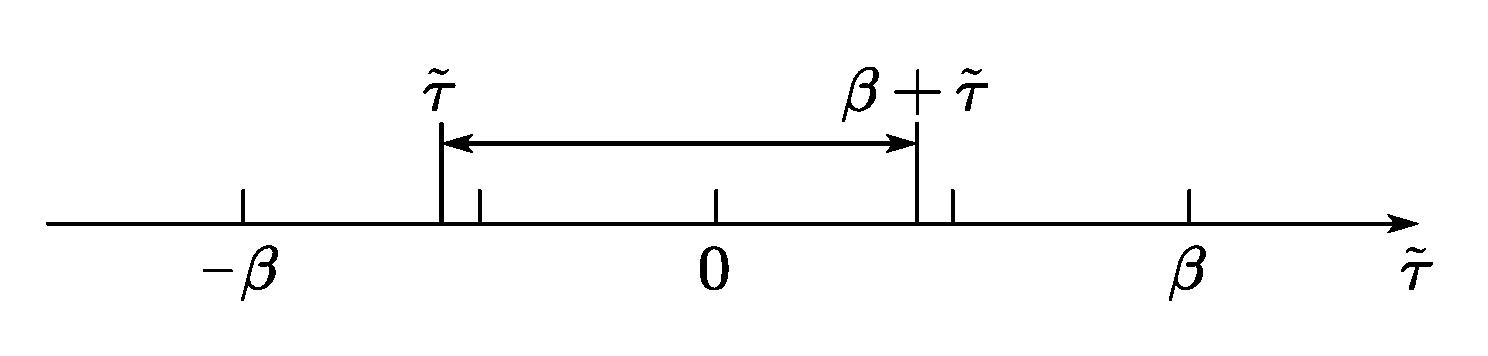
\includegraphics[width=8.5cm]{figure/period.pdf}
    \caption{松原格林函数的周期性(反周期性).}
    \label{period}
\end{figure}
\\下面来证明这一关系.
\begin{proof}
由松原格林函数的定义式:
\begin{equation}
\mathcal{G}_{\alpha \beta}\left(\vct{x}, \vct{x}^{\prime} ; \tilde{\tau}\right)=-\operatorname{Tr}\left[\e^{\beta(\Omega-\hat{K})} \hat{T}_\tau\left[\hat{\psi}^{}_{H \alpha}(\vct{x}, \tilde{\tau}) \hat{\psi}_{H\beta}^{\dagger}\left(\vct{x}^{\prime}\right)\right]\right],
\end{equation}
可以看出由于虚时编时乘积的作用, $\tilde{\tau}>0$ 和 $\tilde{\tau}<0$ 时的松原格林函数的表达式不同, 由此引入了周期性或反周期性. 下面分别讨论这两种情况下松原格林函数的表达式.

(i) $\tau>\tau^{\prime}$, 即 $\tilde{\tau}>0$:
\begin{equation}
\mathcal{G}^{(1)}_{\alpha \beta}\left(\vct{x}, \vct{x}^{\prime} ; \tilde{\tau}\right)  =-\operatorname{Tr}\left[\e^{\beta(\Omega-\hat{K})} \hat{\psi}^{}_{H \alpha}(\vct{x}, \tilde{\tau}) \hat{\psi}_{H\beta}^{\dagger}\left(\vct{x}^{\prime}\right)\right] ;
\end{equation}

(ii) $\tau<\tau^{\prime}$, 即 $\tilde{\tau}<0$:
\begin{align}
\mathcal{G}^{(2)}_{\alpha \beta}\left(\vct{x}, \vct{x}^{\prime} ; \tilde{\tau}\right) & =\mp \operatorname{Tr}\left[\e^{\beta(\Omega-\hat{K})} \hat{\psi}_{H\beta}^{\dagger}\left(\vct{x}^{\prime}\right) \hat{\psi}^{}_{H \alpha}(\vct{x}, \tilde{\tau})\right] \nonumber\\
& =\mp \operatorname{Tr}\left[\e^{\beta(\Omega-\hat{K})} \hat{\psi}_{H\beta}^{\dagger}\left(\vct{x}^{\prime}\right) \e^{\hat{K} \tilde{\tau}} \hat{\psi}^{}_\alpha(\vct{x}) \e^{-\hat{K} \tilde{\tau}}\right]\nonumber \\
& =\mp \operatorname{Tr}\left[\e^{\hat{K} \tilde{\tau}} \hat{\psi}^{}_\alpha(\vct{x}) \e^{-\hat{K} \tilde{\tau}} \e^{\beta(\Omega-\hat{K})} \hat{\psi}_{H\beta}^{\dagger}\left(\vct{x}^{\prime}\right)\right]\nonumber \\
& =\mp \operatorname{Tr}\left[\e^{\beta \Omega} \e^{\hat{K} \tilde{\tau}} \hat{\psi}^{}_\alpha(\vct{x}) \e^{-\hat{K}(\tilde{\tau}+\beta)} \hat{\psi}_{H\beta}^{\dagger}\left(\vct{x}^{\prime}\right)\right] \nonumber\\
& =\mp \operatorname{Tr}\left[\e^{\beta(\Omega-\hat{K})} \e^{\hat{K}(\tilde{\tau}+\beta)} \hat{\psi}^{}_\alpha(\vct{x}) \e^{-\hat{K}(\tilde{\tau}+\beta)} \hat{\psi}_{H\beta}^{\dagger}\left(\vct{x}^{\prime}\right)\right] \nonumber\\
& =\mp \operatorname{Tr}\left[\e^{\beta(\Omega-\hat{K})}  \hat{\psi}^{}_{H\alpha}(\vct{x},\beta+ \tilde{\tau})  \hat{\psi}_{H\beta}^{\dagger}\left(\vct{x}^{\prime}\right)\right]\nonumber \\
& =\pm \mathcal{G}^{(1)}_{\alpha \beta}\left(\vct{x}, \vct{x}^{\prime} ; \tilde{\tau}+\beta\right) .
\end{align}
这样就证明了松原格林函数的周期性(反周期性).
\end{proof}

\subsection{松原格林函数对“虚时”的傅里叶变换}
与零温格林函数的傅里叶变换不同, 有限温格林函数中的 “虚时” $\tau$ 是在 $[-\beta, \beta]$ 区间内变换, 而且具有周期性或反周期性. 零温格林函数中的时间是从 $(-\infty,+\infty)$ 区间内变换, 所以可以引入平面波表象进行连续的傅里叶变换. 而有限温格林函数需要进行分立的傅里叶变换, 引入如下在 $[-\beta, \beta]$ 区间内完备的波函数(三角函数基):
\begin{equation}
\psi_n(\tau)=\frac{1}{\sqrt{2 \beta}} \e^{-\ii \omega_n \tau}, \quad \omega_n=\frac{n \pi}{\beta}, \quad n=0, \pm 1, \pm 2, \cdots .
\end{equation}
这一组完备波函数满足如下正交关系和完备关系:
\begin{equation}
\left\{\begin{aligned}
\int_{-\beta}^\beta \psi_{n^{\prime}}^*(\tau) \psi^{}_n(\tau) \mathrm{d} \tau & =\delta_{n n^{\prime}}, \\
\sum_n \psi_n^*\left(\tau^{\prime}\right) \psi^{}_n(\tau) & =\delta\left(\tau-\tau^{\prime}\right) .
\end{aligned}\right.
\end{equation}

暂时忽略坐标和自旋, 松原格林函数的傅里叶变换(傅里叶级数展开)定义为:
\begin{equation}
\mathcal{G}(\tau)=\frac{1}{\beta} \sum_n \mathcal{G}\left(\ii \omega_n\right) \e^{-\ii \omega_n \tau},
\end{equation}
相应逆变换(傅里叶变换的分量)为:
\begin{equation}
\mathcal{G}\left(\ii \omega_n\right)=\frac{1}{2} \int_{-\beta}^\beta \mathcal{G}(\tau) \e^{\ii \omega_n \tau}\mathrm{d} \tau .
\end{equation}
进一步考虑 $\mathcal{G}(\tau)$ 的分段性质可以得到:
\begin{equation}
\mathcal{G}\left(\ii \omega_n\right)=\frac{1}{2} \int_{-\beta}^0 \mathcal{G}^{(2)}(\tau) \e^{\ii \omega_n \tau} \mathrm{d} \tau+\frac{1}{2} \int_0^\beta \mathcal{G}^{(1)}(\tau) \e^{\ii \omega_n \tau} \mathrm{d} \tau,
\end{equation}
利用(反)周期性上式第一项可以写为:
\begin{align}
\frac{1}{2} \int_{-\beta}^0 \mathcal{G}^{(2)}(\tau) \e^{\ii \omega_n \tau} \mathrm{d} \tau  =&\pm \frac{1}{2} \int_{-\beta}^0 \mathcal{G}^{(1)}(\tau+\beta) \e^{\ii \omega_n \tau} \mathrm{d} \tau \nonumber\\
\stackrel{\tau^{\prime}=\tau+\beta}{\longrightarrow} & \pm \frac{1}{2} \int_0^\beta \mathcal{G}^{(1)}\left(\tau^{\prime}\right) \e^{\ii \omega_n\left(\tau^{\prime}-\beta\right)} \mathrm{d} \tau^{\prime}\nonumber \\
=&\pm \frac{1}{2} \e^{-\ii \omega_n \beta} \int_0^\beta \mathcal{G}^{(1)}(\tau) \e^{\ii \omega_n \tau}\mathrm{d} \tau ,
\end{align}
这样我们可以只用 $\tau>0$ 时的松原格林函数 $\mathcal{G}^{(1)}(\tau)$ 表示 $\mathcal{G}\left(\ii \omega_n\right)$ :
\begin{align}
\mathcal{G}\left(\ii \omega_n\right) & =\frac{1}{2} \int_0^{\beta} \mathcal{G}^{(1)}(\tau) \e^{\ii \omega_n \tau} \mathrm{d} \tau \pm \frac{1}{2} \e^{-\ii \omega_n \beta}  \int_0^\beta \mathcal{G}^{(1)}(\tau) \e^{\ii \omega_n \tau} \mathrm{d} \tau \nonumber\\
& =\frac{1}{2}\left(1 \pm \e^{-\ii \omega_n \beta}\right) \int_0^\beta \mathcal{G}^{(1)}(\tau) \e^{\ii \omega_n \tau}\mathrm{d} \tau\nonumber\\
& =\frac{1}{2}\left(1 \pm \e^{-\ii \frac{n\pi}{\beta}\beta}\right) \int_0^\beta \mathcal{G}^{(1)}(\tau) \e^{\ii \omega_n \tau}\mathrm{d} \tau\nonumber\\
& =\frac{1}{2}\left[1 \pm(-1)^n\right] \int_0^\beta \mathcal{G}^{(1)}(\tau) \e^{\ii \omega_n \tau}\mathrm{d} \tau.
\end{align}

对于玻色子和费米子, 分别有:
\begin{itemize}
\item 玻色子: $n$ 为偶数时, $\mathcal{G}\left(\ii \omega_n\right)$ 可能不为零;
\item 费米子: $n$ 为奇数时, $\mathcal{G}\left(\ii \omega_n\right)$ 可能不为零.
\end{itemize}
故最终可以得到:
\begin{equation}
\mathcal{G}\left(\ii \omega_n\right)=\int_0^\beta   \mathcal{G}^{(1)}(\tau) \e^{\ii \omega_n \tau}\mathrm{d}\tau,
\end{equation}
由于 $\mathcal{G}(\tau)$ 在 $[0, \beta]$ 区间内就是 $\mathcal{G}^{(1)}(\tau)$, 所以上式还可以更一般地写为:
\begin{equation}
\mathcal{G}\left(\ii \omega_n\right)=\int_0^\beta   \mathcal{G}(\tau) \e^{\ii \omega_n \tau}\mathrm{d}\tau,
\end{equation}
其中
\begin{equation}
\omega_n=\left\{\begin{aligned}
&\frac{2 n \pi}{\beta} &\text{(玻色子);} \\
&\frac{(2 n+1) \pi}{\beta}& \text {(费米子),}
\end{aligned}\quad n=0, \pm 1, \pm 2, \cdots .\right.
\end{equation}

\section{自由粒子的松原格林函数}
自由粒子系统的单粒子零温格林函数在微扰计算中十分重要, 同样, 自由粒子系统的松原格林函数在微扰计算中也是十分重要, 下面计算其具体的形式.

自由粒子体系的哈密顿量可以在平面波表象下写成如下二次量子化的形式:
\begin{equation}
\hat{H}=\hat{H}_0=\sum_{k \sigma} \epsilon_k^0 \hat{C}_{k \sigma}^{\dagger} \hat{C}^{}_{k \sigma}.
\end{equation}
有限温度下, 有:
\begin{equation}
\hat{K}=\hat{K}_0=\hat{H}_0-\mu \hat{N}=\sum_{k \sigma}\left(\epsilon_k^0-\mu\right) \hat{C}_{k \sigma}^{\dagger} \hat{C}^{}_{k \sigma},
\end{equation}
薛定谔绘景下的场算符也可以用平面波展开为:
\begin{equation}
\left\{\begin{aligned}
\hat{\psi}_\alpha(\vct{x})&=\frac{1}{\sqrt{V}} \sum_k \e^{\ii \vct{k} \cdot \vct{x}} \hat{C}_{k \alpha}, \\
\hat{\psi}_\beta^{\dagger}(\vct{x})&=\frac{1}{\sqrt{V}} \sum_k \e^{-\ii \vct{k} \cdot \vct{x}} \hat{C}_{k \beta}^{\dagger},
\end{aligned}\right.
\end{equation}
而有限温度下, 海森堡绘景中的场算符可以写作:
\begin{equation}
\left\{\begin{aligned}
\hat{\psi}_{H \alpha}(\vct{x}, \tau)&=\e^{\hat{K}_0 \tau} \hat{\psi}_\alpha(\vct{x}) \e^{-\hat{K}_0 \tau}, \\
\hat{\psi}_{H \beta}^{\dagger}(\vct{x}, \tau)&=\e^{\hat{K}_0 \tau} \hat{\psi}_\beta^{\dagger}(\vct{x}) \e^{-\hat{K}_0 \tau},
\end{aligned}\right.
\end{equation}
把 $\hat{\psi}_\alpha(\vct{x})$ 和 $\hat{\psi}_\alpha^{\dagger}(\vct{x})$ 的平面波展开代入到上式, 利用算符间的对易关系得到:
\begin{align}
\hat{\psi}_{H \alpha}(\vct{x}, \tau)&=\frac{1}{\sqrt{V}} \sum_k \e^{\ii \vct{k} \cdot \vct{x}} \e^{\hat{K}_0 \tau} \hat{C}_{k \alpha} \e^{-\hat{K}_0 \tau}\nonumber\\
&=\frac{1}{\sqrt{V}} \sum_k \e^{\ii \vct{k} \cdot \vct{x}} \hat{C}_{k \alpha} \e^{-\left(\epsilon_k^0-\mu\right) \tau} \nonumber\\
&=\frac{1}{\sqrt{V}} \sum_k  \hat{C}_{k \alpha} \e^{\ii \vct{k} \cdot \vct{x}-\left(\epsilon_k^0-\mu\right) \tau};\\
\hat{\psi}_{H \beta}^{\dagger}(\vct{x}, \tau)&=\frac{1}{\sqrt{V}} \sum_k \e^{-\ii \vct{k} \cdot \vct{x}} \e^{\hat{K}_0 \tau} \hat{C}_{k \beta}^{\dagger} \e^{-\hat{K}_0 \tau}\nonumber\\
&=\frac{1}{\sqrt{V}} \sum_k \e^{-\ii \vct{k} \cdot \vct{x}} \hat{C}_{k \beta}^{\dagger} \e^{\left(\epsilon_k^0-\mu\right) \tau}\nonumber\\
&=\frac{1}{\sqrt{V}} \sum_k  \hat{C}_{k \beta}^{\dagger} \e^{-\ii \vct{k} \cdot \vct{x}+\left(\epsilon_k^0-\mu\right) \tau} .
\end{align}

由松原格林函数的定义式可以得到自由粒子体系的松原格林函数:
\begin{align}
\mathcal{G}_{\alpha \beta}^0\left(\vct{x}, \tau ; \vct{x}^{\prime}, \tau^{\prime}\right)= & -\operatorname{Tr}\left[\e^{\beta\left(\Omega_0-\hat{K}_0\right)} \hat{T}_\tau\left[\hat{\psi}^{}_{H \alpha}(\vct{x}, \tau) \hat{\psi}_{H \beta}^{\dagger}\left(\vct{x}^{\prime}, \tau^{\prime}\right)\right]\right] \nonumber\\
= & -\theta\left(\tau-\tau^{\prime}\right) \operatorname{Tr}\left[\e^{\beta\left(\Omega_0-\hat{K}_0\right)} \hat{\psi}^{}_{H \alpha}(\vct{x}, \tau) \hat{\psi}_{H \beta}^{\dagger}\left(\vct{x}^{\prime}, \tau^{\prime}\right)\right]\nonumber \\
& \mp \theta\left(\tau^{\prime}-\tau\right) \operatorname{Tr}\left[\e^{\beta\left(\Omega_0-\hat{K}_0\right)} \hat{\psi}_{H \beta}^{\dagger}\left(\vct{x}^{\prime}, \tau^{\prime}\right) \hat{\psi}^{}_{H \alpha}(\vct{x}, \tau)\right] .
\end{align}
利用有限温度下海森堡绘景中场算符的平面波展开, 我们可以分别计算上式中的两项. 首先计算第一项:
\begin{equation}
\begin{aligned}
& -\theta\left(\tau-\tau^{\prime}\right) \operatorname{Tr}\left[\e^{\beta\left(\Omega_0-\hat{K}_0\right)} \hat{\psi}^{}_{H \alpha}(\vct{x}, \tau) \hat{\psi}_{H \beta}^{\dagger}\left(\vct{x}^{\prime}, \tau^{\prime}\right)\right] \\
= & -\theta\left(\tau-\tau^{\prime}\right) \frac{1}{V} \sum_k \sum_{k^{\prime}} \e^{\ii \vct{k} \cdot \vct{x}} \e^{-\ii \vct{k}^{\prime} \cdot \vct{x}^{\prime}} \e^{-\left(\epsilon_k^0-\mu\right) \tau} \e^{\left(\epsilon_{k^{\prime}}^0-\mu\right) \tau^{\prime}} \operatorname{Tr}\left[\e^{\beta\left(\Omega_0-\hat{K}_0\right)} \hat{C}^{}_{k \alpha} \hat{C}_{k^\prime \beta}^{\dagger}\right],
\end{aligned}
\end{equation}
其中:
\begin{equation}
\operatorname{Tr}\left[\e^{\beta\left(\Omega_0-\hat{K}_0\right)} \hat{C}^{}_{k \alpha} \hat{C}_{k^\prime \beta}^{\dagger}\right]=\left\langle\hat{C}^{}_{k \alpha} \hat{C}_{k^\prime \beta}^{\dagger}\right\rangle_T=\delta_{\alpha \beta} \delta_{{k} k^{\prime}}\left\langle 1 \pm \hat{n}_k\right\rangle_0=\delta_{\alpha \beta} \delta_{{k} {k}^{\prime}}\left(1 \pm n_k^0\right),
\end{equation}
这里 $n_k^0$ 是自由粒子体系的单粒子分布函数:
\begin{equation}
n_k^0=\frac{1}{\e^{\beta\left(\epsilon_k^0-\mu\right)} \mp 1} .
\end{equation}
这样第一项可以写为:
\begin{equation}
-\theta\left(\tau-\tau^{\prime}\right) \frac{1}{V} \sum_k \e^{\ii \vct{k} \cdot\left(\vct{x}-\vct{x}^{\prime}\right)} \e^{-\left(\epsilon_k^0-\mu\right)\left(\tau-\tau^{\prime}\right)} \delta_{\alpha \beta}\left(1 \pm n_k^0\right).
\end{equation}
与第一项的计算过程完全相同, 第二项可以写为:
\begin{equation}
\mp \theta\left(\tau^{\prime}-\tau\right) \frac{1}{V} \sum_k \e^{\ii \vct{k} \cdot\left(\vct{x}-\vct{x}^{\prime}\right)} \e^{-\left(\epsilon_k^0-\mu\right)\left(\tau-\tau^{\prime}\right)} \delta_{\alpha \beta} n_k^0.
\end{equation}
故自由粒子的松原格林函数可以表示为:
\begin{align}
\mathcal{G}_{\alpha \beta}^0\left(\vct{x}, \tau ; \vct{x}^{\prime}, \tau^{\prime}\right)=& -\theta\left(\tau-\tau^{\prime}\right) \frac{1}{V} \sum_k \e^{\ii \vct{k} \cdot\left(\vct{x}-\vct{x}^{\prime}\right)} \e^{-\left(\epsilon_k^0-\mu\right)\left(\tau-\tau^{\prime}\right)} \delta_{\alpha \beta}\left(1 \pm n_k^0\right) \nonumber\\
& \mp \theta\left(\tau^{\prime}-\tau\right) \frac{1}{V} \sum_k \e^{\ii \vct{k} \cdot\left(\vct{x}-\vct{x}^{\prime}\right)} \e^{-\left(\epsilon_k^0-\mu\right)\left(\tau-\tau^{\prime}\right)} \delta_{\alpha \beta} n_k^0 .
\end{align}

考虑粒子数算符的平均值:
\begin{align}
\langle\hat{N}\rangle_T & =\mp \sum_\alpha \int \mathrm{d} \vct{x} \lim _{\substack{\vct{x}^{\prime} \rightarrow \vct{x} \\
\tau^{\prime} \rightarrow \tau^{+}}} \mathcal{G}_{\alpha \alpha}^0\left(\vct{x}, \tau ; \vct{x}^{\prime}, \tau^{\prime}\right) \nonumber\\
& =\mp \sum_\alpha \int \mathrm{d} \vct{x} \lim _{\substack{\vct{x}^{\prime} \rightarrow \vct{x} \\
\tau^{\prime} \rightarrow \tau^{+}}}\left[\mp \frac{1}{V} \sum_k \e^{\ii \vct{k} \cdot\left(\vct{x}-\vct{x}^{\prime}\right)} \e^{-\left(\epsilon_k^0-\mu\right)\left(\tau-\tau^{\prime}\right)} \delta_{\alpha \alpha } n_k^0\right] \nonumber\\
& =\sum_{ \alpha}\sum_{k} \frac{1}{V} \int \mathrm{d} \vct{x} n_k^0 \nonumber\\
& =\sum_{ \alpha}\sum_{k} n_k^0 .
\end{align}
注意这里 $\tau^{\prime} \rightarrow \tau^{+}>\tau$, 所以只需考虑第二项. 同样地, 内能的平均值可以写为:
\begin{align}
\langle E\rangle_T=&\langle\hat{H}\rangle_T=\langle\hat{H}_0\rangle_T\nonumber\\
=&\mp \frac{1}{2} \sum_\alpha \int \mathrm{d} \vct{x} \lim _{\substack{\vct{x}^{\prime} \rightarrow \vct{x} \\ \tau^{\prime} \rightarrow \tau^{+}}}\left[-\frac{\partial}{\partial \tau}-\frac{\nabla_{\vct x}^2}{2 m}+\mu\right] \mathcal{G}^0_{\alpha \alpha}\left(\vct{x}, \tau ; \vct{x}^{\prime}, \tau^{\prime}\right)\nonumber\\
=&\mp \frac{1}{2} \sum_\alpha \int \mathrm{d} \vct{x} \lim _{\substack{\vct{x}^{\prime} \rightarrow \vct{x} \\ \tau^{\prime} \rightarrow \tau^{+}}}\left[-\frac{\partial}{\partial \tau}-\frac{\nabla_{\vct x}^2}{2 m}+\mu\right]\left[\mp \frac{1}{V} \sum_k \e^{\ii \vct{k} \cdot\left(\vct{x}-\vct{x}^{\prime}\right)} \e^{-\left(\epsilon_k^0-\mu\right)\left(\tau-\tau^{\prime}\right)} n_k^0\right] \nonumber\\
=& \frac{1}{2}\frac{1}{V}\sum_\alpha\sum_k\int \mathrm{d} \vct{x}\lim _{\substack{\vct{x}^{\prime} \rightarrow \vct{x} \\ \tau^{\prime} \rightarrow \tau^{+}}} \left[\left(\epsilon_k^0-\mu\right)-\frac{(\ii \vct{k})^2}{2 m}+\mu\right]\left[\e^{\ii \vct{k} \cdot\left(\vct{x}-\vct{x}^{\prime}\right)} \e^{-\left(\epsilon_k^0-\mu\right)\left(\tau-\tau^{\prime}\right)}\right]n_k^0\nonumber\\
=& \frac{1}{2}\frac{1}{V}\sum_\alpha\sum_k\int \mathrm{d} \vct{x}\left[\left(\epsilon_k^0-\mu\right)+\epsilon_k^0+\mu\right]n_k^0\nonumber\\
=&\sum_\alpha\sum_k\epsilon_k^0 n_k^0 .
\end{align}

考虑自由粒子体系松原格林函数的傅里叶变换:
\begin{equation}
\mathcal{G}_{\alpha \beta}^0\left(\vct{x}, \tau ; \vct{x}^{\prime}, \tau^{\prime}\right)=\frac{1}{V} \sum_k  \frac{1}{\beta} \sum_n\e^{\ii \vct{k} \cdot\left(\vct{x}-\vct{x}^{\prime}\right)} \e^{-\ii \omega_n\left(\tau-\tau^{\prime}\right)} \mathcal{G}_{\alpha \beta}^0(\vct{k}, \ii \omega_n),
\end{equation}
其逆变换为:
\begin{equation}
\mathcal{G}_{\alpha \beta}^0(\vct{k}, \ii \omega_n)=\int \mathrm{d}\left(\vct{x}-\vct{x}^{\prime}\right)\int_0^\beta \mathrm{d}\left(\tau-\tau^{\prime}\right) \e^{-\ii \vct{k} \cdot\left(\vct{x}-\vct{x}^{\prime}\right)}  \e^{\ii \omega_n\left(\tau-\tau^{\prime}\right)} \mathcal{G}_{\alpha \beta}^0\left(\vct{x}, \tau ; \vct{x}^{\prime}, \tau^{\prime}\right)
\end{equation}
只需考虑 $\tau>\tau^{\prime}$ 的情况, 也就是在傅里叶变换中只需考虑前面计算得到的第一项:
\begin{align}
\mathcal{G}_{\alpha \beta}^0(\vct{k}, \ii \omega_n) =&-\frac{\delta_{\alpha \beta}}{V} \int \mathrm{d}\left(\vct{x}-\vct{x}^{\prime}\right) \e^{-\ii \vct{k} \cdot\left(\vct{x}-\vct{x}^{\prime}\right)} \int_0^\beta \mathrm{d}\left(\tau-\tau^{\prime}\right) \e^{\ii \omega_n\left(\tau-\tau^{\prime}\right)} \nonumber\\
&\sum_{k^{\prime}} \e^{\ii \vct{k}^{\prime} \cdot\left(\vct{x}-\vct{x}^{\prime}\right)} \e^{-\left(\epsilon_{k^{\prime}}^0-\mu\right)\left(\tau-\tau^{\prime}\right)}\left(1 \pm n_{k^{\prime}}^0\right) \nonumber\\
=&-\delta_{\alpha \beta} \int_0^\beta  \mathrm{d}\left(\tau-\tau^{\prime}\right)\e^{\left[\ii \omega_n-\left(\epsilon_k^0-\mu\right)\right]\left(\tau-\tau^{\prime}\right)}\left(1 \pm n_k^0\right) \nonumber\\
=&-\left.\frac{\delta_{\alpha \beta}}{\ii \omega_n-\left(\epsilon_k^0-\mu\right)} \e^{\left[\ii \omega_n-\left(\epsilon_k^0-\mu\right)\right]\left(\tau-\tau^{\prime}\right)}\right|_{\tau-\tau^{\prime}=0} ^\beta\left(1 \pm n_k^0\right) \nonumber\\
=&-\frac{\delta_{\alpha \beta}}{\ii \omega_n-\left(\epsilon_k^0-\mu\right)}\left\{\e^{\left[\ii \omega_n-\left(\epsilon_k^0-\mu\right)\right] \beta}-1\right\}\left(1 \pm n_k^0\right) .
\end{align}
分两种情况讨论:
\begin{itemize}
\item 玻色子. 此时 $\omega_n=\frac{2 n \pi}{\beta}, n=0, \pm 1, \pm 2, \cdots, \e^{\ii \omega_n \beta}=1$, 有:
\begin{equation}
\left\{\e^{\left[\ii \omega_n-\left(\epsilon_k^0-\mu\right)\right] \beta}-1\right\}\left(1+n_k^0\right)=\left[\e^{-\left(\epsilon_k^0-\mu\right) \beta}-1\right]\left[1+\frac{1}{\e^{\beta\left(\epsilon_k^0-\mu\right)}-1}\right]=-1 .
\end{equation}
\item 费米子. 此时 $\omega_n=\frac{(2 n+1) \pi}{\beta}, n=0, \pm 1, \pm 2, \cdots, \e^{\ii \omega_n \beta}=-1$, 有:
\begin{equation}
\left\{\e^{\left[\ii \omega_n-\left(\epsilon_k^0-\mu\right)\right] \beta}-1\right\}\left(1-n_k^0\right)=\left[-\e^{-\left(\epsilon_k^0-\mu\right) \beta}-1\right]\left[1-\frac{1}{\e^{\beta\left(\epsilon_k^0-\mu\right)}+1}\right]=-1 .
\end{equation}
\end{itemize}
两种情况结果相同, 可以得到一个统一的表达式:
\begin{equation}
\mathcal{G}_{\alpha \beta}^0(\vct{k}, \ii \omega_n)=\frac{\delta_{\alpha \beta}}{\ii \omega_n-\left(\epsilon_k^0-\mu\right)},
\end{equation}
这是之后费曼图展开后的基本单元.

\section{松原格林函数的 Lehmann 表示}
为了进一步考虑松原格林函数的解析性质, 我们引入松原格林函数的 Lehmann 表示. 和零温情况一样, 松原格林函数的 Lehmann 表示也是考虑均匀的系统, 即$[\hat{H}, \hat{\vct{P}}]_{-}=0$, 存在一组完备力学量组 $\{\hat{H}, \hat{N}, \hat{\vct{P}}\}$, 它们彼此对易, 存在一组共同的本征态 $\{|n\rangle\}=\left\{\left|E_n, N_n, \vct{P}_n\right\rangle\right\}$, 满足如下关系:
\begin{equation}
\hat{H}|n\rangle=E_n|n\rangle, \quad \hat{N}|n\rangle=N_n|n\rangle, \quad \hat{\vct{P}}|n\rangle=\vct{P}_n|n\rangle.
\end{equation}
在有限温情况下, 我们通常考虑 $\hat{K}=\hat{H}-\mu \hat{N}$, 用它代替 $\hat{H}$ 有:
\begin{equation}
\hat{K}|n\rangle=(\hat{H}-\mu \hat{N})|n\rangle=\left(E_n-\mu N_n\right)|n\rangle=K_n|n\rangle .
\end{equation}
和零温时计算 Lehmann 表示相同, 我们在格林函数中插入一组完备关系. 不同的是, 零温时只考虑基态平均, 但在有限温的情况下需要考虑对所有可能状态的量子统计平均. 由定义式, 有:
\begin{align}
\mathcal{G}_{\alpha \beta}\left(\vct{x}, \tau ; \vct{x}^{\prime}, \tau^{\prime}\right)= & -\left\langle\hat{T}_\tau\left[\hat{\psi}^{}_{H \alpha}(\vct{x}, \tau) \hat{\psi}_{H \beta}^{\dagger}\left(\vct{x}^{\prime}, \tau^{\prime}\right)\right]\right\rangle_T \nonumber\\
= & -\operatorname{Tr}\left[\e^{\beta(\Omega-\hat{K})} \hat{T}_\tau\left[\hat{\psi}^{}_{H \alpha}(\vct{x}, \tau) \hat{\psi}_{H \beta}^{\dagger}\left(\vct{x}^{\prime}, \tau^{\prime}\right)\right]\right]\nonumber \\
= & -\theta\left(\tau-\tau^{\prime}\right) \sum_n\left\langle n\left|\e^{\beta(\Omega-\hat{K})} \hat{\psi}^{}_{H \alpha}(\vct{x}, \tau) \hat{\psi}_{H \beta}^{\dagger}\left(\vct{x}^{\prime}, \tau^{\prime}\right)\right| n\right\rangle\nonumber \\
& \mp \theta\left(\tau^{\prime}-\tau\right) \sum_n\left\langle n\left|\e^{\beta(\Omega-\hat{K})} \hat{\psi}^{\dagger}_{H \beta}\left(\vct{x}^{\prime}, \tau^{\prime}\right) \hat{\psi}^{}_{H\alpha}(\vct{x}, \tau)\right| n\right\rangle \nonumber\\
\equiv & I_1+I_2 .
\end{align}
先考虑第一项, 有:
\begin{align}
I_1 & =-\theta\left(\tau-\tau^{\prime}\right) \sum_n\left\langle n\left|\e^{\beta(\Omega-\hat{K})} \hat{\psi}^{}_{H \alpha}(\vct{x}, \tau) \hat{\psi}_{H\beta}^{\dagger}\left(\vct{x}^{\prime}, \tau^{\prime}\right)\right| n\right\rangle \nonumber\\
& =-\theta\left(\tau-\tau^{\prime}\right) \sum_{m n}\left\langle n\left|\e^{\beta(\Omega-\hat{K})} \hat{\psi}^{}_{H \alpha}(\vct{x}, \tau)\right| m\right\rangle\left\langle m\left|\hat{\psi}_{H \beta}^{\dagger}\left(\vct{x}^{\prime}, \tau^{\prime}\right)\right| n\right\rangle \nonumber\\
& =-\theta\left(\tau-\tau^{\prime}\right) \e^{\beta \Omega} \sum_{m n} \e^{-K_n \beta}\left\langle n\left| \hat{\psi}^{}_{H \alpha}(\vct{x}, \tau)\right| m\right\rangle\left\langle m\left|\hat{\psi}_{H \beta}^{\dagger}\left(\vct{x}^{\prime}, \tau^{\prime}\right)\right| n\right\rangle ,
\end{align}
下面计算两矩阵元. 有限温度下, 海森堡绘景中的场算符可以写作:
\begin{equation}
\hat{\psi}_{H \alpha}(\vct{x}, \tau)=\e^{\hat{K} \tau} \hat{\psi}_\alpha(\vct{x}) \e^{-\hat{K} \tau}, 
\end{equation}
其中 $\hat{\psi}_\alpha(\vct{x})$ 是薛定谔绘景下的场算符, 可以用平面波展开为:
\begin{equation}
\hat{\psi}_\alpha(\vct{x})=\frac{1}{\sqrt{V}} \sum_k \e^{\ii \vct{k} \cdot \vct{x}} \hat{C}_{k \alpha}, 
\end{equation}
取 $x=0$, 有
\begin{equation}
\hat{\psi}_\alpha(0)=\frac{1}{\sqrt{V}} \sum_k  \hat{C}_{k \alpha}.
\end{equation}
由总动量算符的定义
\begin{equation}
\hat{\vct{P}}  =\sum_{k \alpha} \vct{k} \hat{C}_{k \alpha}^{\dagger} \hat{C}^{}_{k \alpha} ,
\end{equation}
可以得到
\begin{equation}
 \e^{-\ii \hat{\vct{P}} \cdot \vct{x}} \hat{C}_{k \alpha} \e^{\ii \hat{\vct{P}} \cdot \vct{x}}=\hat{C}_{k \alpha} \e^{\ii \vct{k} \cdot \vct{x}} .
\end{equation}
\begin{proof}
利用 Campbell-Baker-Hausdorff 公式:
\begin{equation}
\e^A B \e^{-A}=B+[A, B]_-+\frac{1}{2 !}[A,[A, B]_-]_-+\frac{1}{3 !}[A,[A,[A, B]_-]_-]_-+\cdots ,
\end{equation}
这里令 $A=-\ii \hat{\vct{P}} \cdot \vct{x}$, $B=\hat{C}_{k \alpha}$,
则
\begin{align}
  \e^{-\ii \hat{\vct{P}} \cdot \vct{x}} \hat{C}_{k \alpha} \e^{\ii \hat{\vct{P}} \cdot \vct{x}}&=\hat{C}_{k \alpha}+\left[-\ii \hat{\vct{P}} \cdot \vct{x}, \hat{C}_{k \alpha}\right]_-+\frac{1}{2 !}\left[-\ii \hat{\vct{P}} \cdot \vct{x} ,\left[-\ii \hat{\vct{P}} \cdot \vct{x}, \hat{C}_{k \alpha}\right]_-\right]_-+\cdots \nonumber\\
& =\hat{C}_{k \alpha}+(-\ii \vct{x})\left[\hat{\vct{P}}, \hat{C}_{k \alpha}\right]_-+\frac{1}{2 !}(-\ii \vct{x})^2\left[\hat{\vct{P}},\left[\hat{\vct{P}}, \hat{C}_{k \alpha}\right]_-\right]_-+\cdots ,
\end{align}
其中:
\begin{align}
\left[\hat{\vct{P}}, \hat{C}^{}_{k \alpha}\right]_-&=\sum_{k^{\prime} \alpha^{\prime}} \vct{k}^\prime\left[\hat{C}_{k^{\prime} \alpha^{\prime}}^{\dagger} \hat{C}^{}_{k^{\prime} \alpha^{\prime}}, \hat{C}^{}_{k \alpha}\right]_- \nonumber\\
& =\sum_{k^\prime \alpha^{\prime}} \vct{k}^{\prime}\left[\hat{C}_{k^{\prime} \alpha^{\prime}}^{\dagger}, \hat{C}^{}_{k \alpha}\right]_- \hat{C}^{}_{k^{\prime} \alpha^{\prime}} \nonumber\\
& =-\vct{k} \hat{C}_{k \alpha},
\end{align}
代回原表达式中, 有:
\begin{align}
\e^{-\ii \hat{\vct{P}} \cdot \vct{x}} \hat{C}_{k \alpha} \e^{\ii \hat{\vct{P}} \cdot \vct{x}}&=\hat{C}_{k \alpha}+(-\ii \vct{x}) \cdot(-\vct{k}) \cdot \hat{C}_{k \alpha}+\frac{1}{2 !} \cdot(-\ii \vct{x})^2 \cdot(-\vct{k})^{2} \cdot \hat{C}_{k \alpha}+\cdots \nonumber\\
& =\hat{C}_{k \alpha}\left[1+(\ii \vct{x} \cdot \vct{k})+\frac{1}{2 !}(\ii \vct{x} \cdot \vct{k})^2+\cdots\right] \nonumber\\
& =\hat{C}_{k \alpha} \e^{\ii \vct{k} \cdot \vct{x}} ,
\end{align}
即:
\begin{equation}
\e^{-\ii \hat{\vct{P}} \cdot \vct{x}} \hat{C}_{k \alpha} \e^{\ii \hat{\vct{P}} \cdot \vct{x}}=\hat{C}_{k \sigma} \e^{\ii \vct{k} \cdot \vct{x}}.
\end{equation}
\end{proof}
利用上式, 可将薛定谔绘景下的场算符表示为:
\begin{align}
\hat{\psi}_\alpha(\vct{x}) & =\frac{1}{\sqrt{V}} \sum_{k } \hat{C}_{k \alpha} \e^{\ii \vct{k} \cdot \vct{x}}\nonumber\\
&=\frac{1}{\sqrt{V}} \sum_{k} \e^{-\ii \hat{\vct{P}} \cdot \vct{x}} \hat{C}_{k \alpha} \e^{\ii \hat{\vct{P}} \cdot \vct{x}}\nonumber\\
&=\e^{-\ii \hat{\vct{P}} \cdot \vct{x}}\left(\frac{1}{\sqrt{V}} \sum_{k} \hat{C}_{k \alpha}\right) \e^{\ii \hat{\vct{P}} \cdot \vct{x}} \nonumber\\
& =\e^{-\ii \hat{\vct{P}} \cdot \vct{x}} \hat{\psi}_\alpha(0) \e^{\ii \hat{\vct{P}} \cdot \vct{x}}.
\end{align}
所以
\begin{align}
\hat{\psi}_{H \alpha}(\vct{x}, \tau)=&\e^{\hat{K} \tau} \hat{\psi}_\alpha(\vct{x}) \e^{-\hat{K} \tau}=\e^{\hat{K} \tau} \e^{-\ii \hat{\vct{P}} \cdot \vct{x}} \hat{\psi}_\alpha(0) \e^{\ii \hat{\vct{P}} \cdot \vct{x}} \e^{-\hat{K} \tau}\nonumber\\
=& \e^{-\ii \hat{\vct{P}} \cdot \vct{x}}\e^{\hat{K} \tau} \hat{\psi}_\alpha(0)\e^{-\hat{K} \tau} \e^{\ii \hat{\vct{P}} \cdot \vct{x}} ,
\end{align}
代入矩阵元中可以得到:
\begin{equation}
\left\langle n\left| \hat{\psi}_{H \alpha}(\vct{x}, \tau)\right| m\right\rangle=\left\langle n\left|\e^{-\ii \hat{\vct{P}} \cdot \vct{x}}\e^{\hat{K} \tau} \hat{\psi}_\alpha(0)\e^{-\hat{K} \tau} \e^{\ii \hat{\vct{P}} \cdot \vct{x}}\right| m\right\rangle=\e^{-\ii \vct{P}_{nm} \cdot \vct{x}}\e^{{K}_{nm} \tau}\left\langle n\left|\hat{\psi}_\alpha(0)\right| m\right\rangle,
\end{equation}
这里定义了
\begin{equation}
K_{n m}\equiv K_n-K_m, \quad \vct{P}_{n m}\equiv \vct{P}_n-\vct{P}_m .
\end{equation}
类似地, 有
\begin{equation}
\hat{\psi}^{\dagger}_{H \beta}(\vct{x}^{\prime}, \tau^{\prime})= \e^{-\ii \hat{\vct{P}} \cdot \vct{x}^{\prime}}\e^{\hat{K} \tau^{\prime}} \hat{\psi}^{\dagger}_\beta(0)\e^{-\hat{K} \tau^{\prime}} \e^{\ii \hat{\vct{P}} \cdot \vct{x}^{\prime}} ,
\end{equation}
\begin{equation}
\left\langle m\left| \hat{\psi}^{\dagger}_{H \beta}(\vct{x}^{\prime}, \tau^{\prime})\right| n\right\rangle=\e^{\ii \vct{P}_{nm} \cdot \vct{x}^{\prime}}\e^{-{K}_{nm} \tau^{\prime}}\left\langle m\left|\hat{\psi}^{\dagger}_\beta(0)\right| n\right\rangle.
\end{equation}
将计算得到的矩阵元表达式带回 $I_1$, 有:
\begin{align}
I_1 =&-\theta\left(\tau-\tau^{\prime}\right) \e^{\beta \Omega} \nonumber\\
&\times\sum_{m n} \e^{-K_n \beta}\e^{-\ii \vct{P}_{nm} \cdot \vct{x}}\e^{{K}_{nm} \tau}\left\langle n\left|\hat{\psi}^{}_\alpha(0)\right| m\right\rangle \e^{\ii \vct{P}_{nm} \cdot \vct{x}^{\prime}}\e^{-{K}_{nm} \tau^{\prime}}\left\langle m\left|\hat{\psi}_\beta^{\dagger}(0)\right| n\right\rangle \nonumber\\
=&-\theta\left(\tau-\tau^{\prime}\right) \e^{\beta \Omega} \sum_{m n} \e^{-K_n \beta}\e^{K_{n m}\left(\tau-\tau^{\prime}\right)} \e^{-\ii \vct{P}_{n m} \cdot\left(\vct{x}-\vct{x}^{\prime}\right)}\left\langle n\left|\hat{\psi}^{}_\alpha(0)\right| m\right\rangle\left\langle m\left|\hat{\psi}_\beta^{\dagger}(0)\right| n\right\rangle \nonumber\\
\xlongequal[]{\text{对调}n, m}&-\theta\left(\tau-\tau^{\prime}\right) \e^{\beta \Omega} \sum_{m n} \e^{-K_m \beta}\e^{-K_{n m}\left(\tau-\tau^{\prime}\right)} \e^{\ii \vct{P}_{n m} \cdot\left(\vct{x}-\vct{x}^{\prime}\right)}\left\langle m\left|\hat{\psi}^{}_\alpha(0)\right| n\right\rangle\left\langle n\left|\hat{\psi}_\beta^{\dagger}(0)\right| m\right\rangle .
\end{align}
注意 $I_1$ 最后表达式中暗含求和中只有 $N_n-N_m=1$ 的项不为零. 同理可以得到:
\begin{equation}
I_2=\mp \theta\left(\tau^{\prime}-\tau\right) \e^{\beta \Omega} \sum_{m n} \e^{-K_n \beta}\e^{K_{n m}\left(\tau^{\prime}-\tau\right)} \e^{-\ii \vct{P}_{n m} \cdot\left(\vct{x}^{\prime}-\vct{x}\right)}\left\langle n\left|\hat{\psi}_\beta^{\dagger}(0)\right| m\right\rangle\left\langle m\left|\hat{\psi}^{}_\alpha(0)\right| n\right\rangle ,
\end{equation}
这里也是 $N_n-N_m=1$ 时的项不为零. 这样可以得到:
\begin{align}
&\mathcal{G}_{\alpha \beta}\left(\vct{x}, \tau ; \vct{x}^{\prime}, \tau^{\prime}\right)\nonumber\\
=&  -\theta\left(\tau-\tau^{\prime}\right) \e^{\beta \Omega} \sum_{m n} \e^{-K_m \beta}\e^{-K_{n m}\left(\tau-\tau^{\prime}\right)} \e^{\ii \vct{P}_{n m} \cdot\left(\vct{x}-\vct{x}^{\prime}\right)} \left\langle m\left|\hat{\psi}^{}_\alpha(0)\right| n\right\rangle\left\langle n\left|\hat{\psi}_\beta^{\dagger}(0)\right| m\right\rangle \nonumber\\
&\mp \theta\left(\tau^{\prime}-\tau\right) \e^{\beta \Omega} \sum_{m n} \e^{-K_n \beta}\e^{K_{n m}\left(\tau^{\prime}-\tau\right)} \e^{-\ii \vct{P}_{n m} \cdot\left(\vct{x}^{\prime}-\vct{x}\right)}\left\langle n\left|\hat{\psi}_\beta^{\dagger}(0)\right| m\right\rangle\left\langle m\left|\hat{\psi}^{}_\alpha(0)\right| n\right\rangle ,
\end{align}
整体只有 $N_n-N_m=1$ 时的项不为零.

下面计算动量空间中的格林函数, 前面已经讨论过松原格林函数的傅里叶变换可以只用 $\tau>\tau^{\prime}$ 的部分表示, 有:
\begin{align}
\mathcal{G}_{\alpha \beta}\left(\vct{k}, \ii \omega_n\right)=&\int_0^\beta \mathrm{d}\left(\tau-\tau^{\prime}\right) \int \mathrm{d}\left(\vct{x}-\vct{x}^{\prime}\right)\e^{\ii \omega_n\left(\tau-\tau^{\prime}\right)}  \e^{-\ii \vct{k} \cdot\left(\vct{x}-\vct{x}^{\prime}\right)}\mathcal{G}_{\alpha \beta}\left(\vct{x}, \tau ; \vct{x}^{\prime}, \tau^{\prime}\right) \nonumber\\
=& -\int_0^\beta \mathrm{d}\left(\tau-\tau^{\prime}\right) \int \mathrm{d}\left(\vct{x}-\vct{x}^{\prime}\right) \e^{\beta \Omega} \sum_{m n} \e^{-K_m \beta}\left\langle m\left|\hat{\psi}_\alpha(0)\right| n\right\rangle\left\langle n\left|\hat{\psi}_\beta^{\dagger}(0)\right| m\right\rangle \nonumber\\
& \times\e^{-K_{n m}\left(\tau-\tau^{\prime}\right)} \e^{\ii \vct{P}_{n m} \cdot\left(\vct{x}-\vct{x}^{\prime}\right)} \e^{-\ii \vct{k} \cdot\left(\vct{x}-\vct{x}^{\prime}\right)} \e^{\ii \omega_n\left(\tau-\tau^{\prime}\right)}\nonumber \\
= & -\int_0^\beta \mathrm{d}\left(\tau-\tau^{\prime}\right) \int \mathrm{d}\left(\vct{x}-\vct{x}^{\prime}\right) \e^{\beta \Omega} \sum_{m n} \e^{-K_m \beta}\left\langle m\left|\hat{\psi}^{}_\alpha(0)\right| n\right\rangle\left\langle n\left|\hat{\psi}_\beta^{\dagger}(0)\right| m\right\rangle \nonumber\\
&  \times\e^{\left(\ii \omega_n-K_{n m}\right)\left(\tau-\tau^{\prime}\right)} \e^{-\ii\left(\vct{k}-\vct{P}_{n m}\right) \cdot\left(\vct{x}-\vct{x}^{\prime}\right)} \nonumber\\
= & -\e^{\beta \Omega} \sum_{m n} \e^{-K_m \beta}(2 \pi)^3 \delta\left(\vct{k}-\vct{P}_{n m}\right)\nonumber\\
& ~~~~~~~~~~~~~~~~~~ \times\left.\left\langle m\left|\hat{\psi}^{}_\alpha(0)\right| n\right\rangle\left\langle n\left|\hat{\psi}_\beta^{\dagger}(0)\right| m\right\rangle \frac{\e^{\left(i \omega_n-K_{n m}\right)\left(\tau-\tau^{\prime}\right)}}{\ii \omega_n-K_{n m}}\right|_{\tau-\tau^{\prime}=0} ^\beta\nonumber \\
= & -(2 \pi)^3 \e^{\beta \Omega} \sum_{m n} \e^{-{K}_m \beta} \delta\left(\vct{k}-\vct{P}_{n m}\right)\left\langle m\left|\hat{\psi}^{}_\alpha(0)\right| n\right\rangle\left\langle n\left|\hat{\psi}_\beta^{\dagger}(0)\right| m\right\rangle \frac{\e^{\left(\ii \omega_n-K_{n m}\right) \beta}-1}{\ii \omega_n-K_{n m}}\nonumber \\
= & (2 \pi)^3 \e^{\beta \Omega} \sum_{m n} \e^{-{K}_m \beta} \delta\left(\vct{k}-\vct{P}_{n m}\right)\left\langle m\left|\hat{\psi}^{}_\alpha(0)\right| n\right\rangle\left\langle n\left|\hat{\psi}_\beta^{\dagger}(0)\right| m\right\rangle \frac{1 \mp \e^{-\beta K_{n m}}}{\ii \omega_n-K_{n m}},
\end{align}
这里最后考虑了对于玻色子体系和费米子体系具体的松原频率. 可以看出相比于零温情况, 有限温度下的松原格林函数的 Lehmann 表示只包含一项, 其形式似乎更简单. 

同样地, 可以引入谱函数:
\begin{align}
A_{\alpha \beta}(\vct{k}, \omega)=(2 \pi)^3 \e^{\beta \Omega} \sum_{m n}& \e^{-{K}_m \beta}\left\langle m\left|\hat{\psi}^{}_\alpha(0)\right| n\right\rangle\left\langle n\left|\hat{\psi}_\beta^{\dagger}(0)\right| m\right\rangle\nonumber\\
& \times\left(1 \mp \e^{-\beta K_{n m}}\right) \delta\left(\vct{k}-\vct{P}_{n m}\right) \delta\left(\omega-K_{n m}\right),
\end{align}
松原格林函数可以用谱函数表示:
\begin{equation}
\mathcal{G}_{\alpha \beta}\left(\vct{k}, \ii \omega_n\right)=\int_{-\infty}^{\infty} \mathrm{d} \omega^{\prime} \frac{A_{\alpha \beta}\left(\vct{k}, \omega^{\prime}\right)}{\ii \omega_n-\omega^{\prime}} .
\end{equation}
如果考虑相互作用与自旋无关, 则有:
\begin{align}
\mathcal{G}\left(\vct{k}, \ii \omega_n\right)=&\frac{1}{2 S+1} \sum_\alpha \mathcal{G}_{\alpha \alpha}\left(\vct{k}, \ii \omega_n\right), \nonumber\\
=&\frac{(2 \pi)^3}{2 S+1}\e^{\beta \Omega}\sum_\alpha \sum_{m n} \e^{-{K}_m \beta}\delta\left(\vct{k}-\vct{P}_{n m}\right)\frac{1 \mp \e^{-\beta K_{n m}}}{\ii \omega_n-K_{n m}}\left|\left\langle m\left|\hat{\psi}(0)\right| n\right\rangle\right|^2,
\end{align}
引入谱函数:
\begin{align}
A(\vct{k}, \omega)=\frac{(2 \pi)^3}{2 S+1}\e^{\beta \Omega}  \sum_\alpha \sum_{m n} &\e^{-{K}_m \beta} \left|\left\langle m\left|\hat{\psi}(0)\right| n\right\rangle\right|^2\nonumber\\
& \times\delta\left(\vct{k}-\vct{P}_{n m}\right)\left(1 \mp \e^{-\beta K_{n m}}\right) \delta\left(\omega-K_{n m}\right),
\end{align}
则松原格林函数可以用谱函数表示为:
\begin{equation}
\mathcal{G}\left(\vct{k}, \ii \omega_n\right)=\int_{-\infty}^{\infty} \mathrm{d} \omega^{\prime} \frac{A\left(\vct{k}, \omega^{\prime}\right)}{\ii \omega_n-\omega^{\prime}} .
\end{equation}
下一节将证明 $A(\vct{k}, \omega)$ 是归一化的. 可以看到, 松原格林函数的 Lehmann 表示与粒子态密度相关.

\section{其他单粒子热力学格林函数(实时)}
引入 Lehmann 表示后可以很方便地讨论有限温度下三个热力学格林函数间的关系以及它们与松原格林函数的关系. 
\subsection{其他单粒子热力学格林函数的定义}
\begin{definition}{因果格林函数}{}
\begin{align}
\ii G_{\alpha \beta}\left(\vct{x}, t ; \vct{x}^{\prime}, t^{\prime}\right)_T &\equiv \operatorname{Tr}\left[\e^{\beta(\Omega-\hat{K})} \hat{T}_t\left[\hat{\psi}^{}_{H \alpha}(\vct{x}, t) \hat{\psi}_{H \beta}^{\dagger}\left(\vct{x}^{\prime}, t^{\prime}\right)\right]\right]\nonumber\\
&=\left\langle \hat{T}_t\left[\hat{\psi}^{}_{H \alpha}(\vct{x}, t) \hat{\psi}_{H \beta}^{\dagger}\left(\vct{x}^{\prime}, t^{\prime}\right)\right]\right\rangle_T.
\end{align}
取 $T\to 0$ 时应得到零温格林函数.
\end{definition}

\begin{definition}{推迟格林函数}{}
\begin{equation}
 G_{\alpha \beta}^R\left(\vct{x}, t ; \vct{x}^{\prime}, t^{\prime}\right) \equiv - \ii\theta\left(t-t^{\prime}\right) \operatorname{Tr}\left[\e^{\beta(\Omega-\hat{K})}\left[\hat{\psi}^{}_{H \alpha}(\vct{x}, t), \hat{\psi}_{H \beta}^{\dagger}\left(\vct{x}^{\prime}, t^{\prime}\right)\right]_{\mp}\right].
\end{equation}
\end{definition}

\begin{definition}{超前格林函数}{}
\begin{equation}
 G_{\alpha \beta}^A\left(\vct{x}, t ; \vct{x}^{\prime}, t^{\prime}\right) \equiv  \ii\theta\left(t^{\prime}-t\right) \operatorname{Tr}\left[\e^{\beta(\Omega-\hat{K})}\left[\hat{\psi}^{}_{H \alpha}(\vct{x}, t), \hat{\psi}_{H \beta}^{\dagger}\left(\vct{x}^{\prime}, t^{\prime}\right)\right]_{\mp}\right].
\end{equation}
\end{definition}

\subsection{其他单粒子热力学格林函数的 Lehmann 表示}
考虑相互作用与自旋无关, 可以得到上述三种单粒子热力学格林函数的 Lehmann 表示.
\begin{itemize}
\item 因果格林函数:
实部与虚部分别为:
\begin{equation}
\left\{\begin{aligned}
\operatorname{Re} G(\vct{k}, \omega)_T&=\mathcal{P} \int_{-\infty}^{\infty} \mathrm{d} \omega^{\prime} \frac{A\left(\vct{k}, \omega^{\prime}\right)}{\omega-\omega^{\prime}} ,\\
\operatorname{Im} G(\vct{k}, \omega)_T&=-\pi A(\vct{k}, \omega) \frac{1 \pm \e^{- \beta\omega}}{1 \mp \e^{-\beta\omega}}=-\pi A(\vct{k}, \omega) \left[\tanh\left(\frac{\beta \omega}{2}\right)\right] ^{\mp 1},
\end{aligned}\right.
\end{equation}
可得到实部与虚部间的关系为:
\begin{equation}
\operatorname{Re} G(\vct{k}, \omega)_T=-\frac{\mathcal{P}}{\pi} \int_{-\infty}^{\infty} \mathrm{d} \omega^{\prime} \frac{\operatorname{Im} G\left(\vct{k}, \omega^{\prime}\right)_T}{\omega-\omega^{\prime}} \left[\tanh \left(\frac{\beta \omega^{\prime}}{2}\right)\right]^{\pm 1} ,
\end{equation}
此即色散关系.
\item 推迟格林函数:
\begin{equation}
 G^R(\vct{k}, \omega)=\int_{-\infty}^{\infty} \mathrm{d} \omega^{\prime} \frac{A\left(\vct{k}, \omega^{\prime}\right)}{\omega-\omega^{\prime}+\ii \eta},
\end{equation}
可得实部与虚部分别为:
\begin{equation}
\left\{\begin{aligned}
\operatorname{Re} G^R(\vct{k}, \omega)&=\mathcal{P} \int_{-\infty}^{\infty} \mathrm{d} \omega^{\prime} \frac{A\left(\vct{k}, \omega^{\prime}\right)}{\omega-\omega^{\prime}},\\
\operatorname{Im} G^R(\vct{k}, \omega)&=-\pi A(\vct{k}, \omega) ,
\end{aligned}\right.
\end{equation}
实部与虚部间的关系为:
\begin{equation}
\operatorname{Re} G^R(\vct{k}, \omega)=-\frac{\mathcal{P}}{\pi} \int_{-\infty}^{\infty} \mathrm{d} \omega^{\prime} \frac{\operatorname{Im} G^R\left(\vct{k}, \omega^{\prime}\right)}{\omega-\omega^{\prime}} .
\end{equation}
\item 超前格林函数:
\begin{equation}
 G^A(\vct{k}, \omega)=\int_{-\infty}^{\infty} \mathrm{d} \omega^{\prime} \frac{A\left(\vct{k}, \omega^{\prime}\right)}{\omega-\omega^{\prime}-\ii \eta},
\end{equation}
可得实部与虚部分别为:
\begin{equation}
\left\{\begin{aligned}
\operatorname{Re} G^A(\vct{k}, \omega)&=\mathcal{P} \int_{-\infty}^{\infty} \mathrm{d} \omega^{\prime} \frac{A\left(\vct{k}, \omega^{\prime}\right)}{\omega-\omega^{\prime}},\\
\operatorname{Im} G^A(\vct{k}, \omega)&=\pi A(\vct{k}, \omega) ,
\end{aligned}\right.
\end{equation}
实部与虚部间的关系为:
\begin{equation}
\operatorname{Re} G^A(\vct{k}, \omega)=\frac{\mathcal{P}}{\pi} \int_{-\infty}^{\infty} \mathrm{d} \omega^{\prime} \frac{\operatorname{Im} G^A\left(\vct{k}, \omega^{\prime}\right)}{\omega-\omega^{\prime}} .
\end{equation}
\end{itemize}
可见, 只要知道了谱函数 $A(\vct{k}, \omega)$, 就能得到所有的格林函数: $G^A(\vct{k}, \omega)$, $G^R(\vct{k}, \omega)$, $G(\vct{k}, \omega)_T$, $\mathcal{G}\left(\vct{k}, \ii \omega_n\right)$. 

\begin{question}{}{}
证明:
\begin{equation}
 G^R(\vct{k}, \omega)=\int_{-\infty}^{\infty} \mathrm{d} \omega^{\prime} \frac{A\left(\vct{k}, \omega^{\prime}\right)}{\omega-\omega^{\prime}+\ii \eta}.
\end{equation}
\end{question}

\subsection{各种单粒子格林函数间的关系}
相互作用与自旋无关时, 不同的格林函数之间满足关系:
\begin{equation}
\left\{\begin{aligned}
G^A(\vct{k}, \omega)&=\left[G^R(\vct{k}, \omega)\right]^*,\\
\operatorname{Re} G(\vct{k}, \omega)_T&=\operatorname{Re} G^R(\vct{k}, \omega)=\operatorname{Re} G^A(\vct{k}, \omega), \\
\operatorname{Im} G(\vct{k}, \omega)_T&=\operatorname{Im} G^R(\vct{k}, \omega)\left[\tanh\left(\frac{\beta \omega}{2}\right)\right] ^{\mp 1}=-\operatorname{Im} G^A(\vct{k}, \omega) \left[\tanh\left(\frac{\beta \omega}{2}\right)\right] ^{\mp 1} .
\end{aligned}\right.
\end{equation}
可以看出松原格林函数与热力学推迟格林函数间有如下关系:
\begin{equation}
G^R(\vct{k}, \omega)=\mathcal{G}\left(\vct{k}, \ii \omega_n \rightarrow \omega+\ii \eta\right)=\int_{-\infty}^{\infty} \mathrm{d} \omega^{\prime} \frac{A\left(\vct{k}, \omega^{\prime}\right)}{\omega-\omega^{\prime}+\ii \eta},
\end{equation}
解析延拓后得到
\begin{equation}
\left\{\begin{aligned}
\mathcal{G}\left(\vct{k}, \ii \omega_n \right)&\left.=G^R(\vct{k}, \omega)\right|_{\omega\to\ii\omega_n \atop(\omega_n>0)},\\
\mathcal{G}\left(\vct{k}, \ii \omega_n \right)&\left.=G^A(\vct{k}, \omega)\right|_{\omega\to\ii\omega_n \atop(\omega_n<0)}.
\end{aligned}\right.
\end{equation}

通常我们先利用有限温度下的费曼图技术得到松原格林函数的解析结果, 进一步得到热力学推迟格林函数, 而后得到全部的热力学格林函数.

最后, 我们证明谱函数 $A(\vct{k}, \omega)$ 是归一化的.
\begin{proof}
一方面, 当相互作用与自旋无关时, 推迟格林函数可表示为:
\begin{equation}
 G^R\left(\vct{x}, t \right) = - \ii\theta(t)\sum\limits_{\alpha}\frac{1}{2S+1}\operatorname{Tr}\left[\e^{\beta(\Omega-\hat{K})}\left[\hat{\psi}^{}_{H \alpha}(\vct{x}, t), \hat{\psi}_{H \alpha}^{\dagger}\left(0,0\right)\right]_{\mp}\right],
\end{equation}
取 $t\to \eta$, 有
\begin{align}
 G^R\left(\vct{x}, \eta \right) =& - \ii\sum\limits_{\alpha}\frac{1}{2S+1}\operatorname{Tr}\left[\e^{\beta(\Omega-\hat{K})}\left[\hat{\psi}^{}_{H \alpha}(\vct{x}, 0), \hat{\psi}_{H \alpha}^{\dagger}\left(0,0\right)\right]_{\mp}\right]\nonumber\\
=&- \ii\sum\limits_{\alpha}\frac{1}{2S+1}\operatorname{Tr}\left[\e^{\beta(\Omega-\hat{K})}\right] \delta(\vct x)\nonumber\\
=&-\ii \delta(\vct x),
\end{align}
做傅里叶变换后得到:
\begin{equation}
 G^R\left(\vct{k}, \eta \right)= \int\mathrm{d}\vct{x}\e^{-\ii\vct{k}\cdot\vct{x}}G^R\left(\vct{x}, \eta \right)=-\ii.
\end{equation}

另一方面, 将推迟格林函数用谱函数表示, 有
\begin{align}
 G^R\left(\vct{k}, \eta \right) =&\frac{1}{2\pi}\int_{-\infty}^{\infty}\mathrm{d}\omega G^R\left(\vct{k}, \omega \right)\e^{-\ii\omega\eta}\nonumber\\
=&\frac{1}{2\pi}\int_{-\infty}^{\infty}\mathrm{d}\omega \left[\int_{-\infty}^{\infty} \mathrm{d} \omega^{\prime} \frac{A\left(\vct{k}, \omega^{\prime}\right)}{\omega-\omega^{\prime}+\ii \eta}\right]\e^{-\ii\omega\eta}\nonumber\\
=&\frac{1}{2\pi}\int_{-\infty}^{\infty}\mathrm{d}\omega^{\prime} A\left(\vct{k}, \omega^{\prime}\right) \int_{-\infty}^{\infty}\mathrm{d} \omega \frac{\e^{-\ii\omega\eta}}{\omega-\omega^{\prime}+\ii \eta}\nonumber\\
=&\frac{1}{2\pi}\int_{-\infty}^{\infty}\mathrm{d}\omega^{\prime}A\left(\vct{k}, \omega^{\prime}\right) (-2\pi \ii)\nonumber\\
=&-\ii  \int_{-\infty}^{\infty}\mathrm{d}\omega^{\prime} A\left(\vct{k}, \omega^{\prime}\right).
\end{align}

比较两式便可得
\begin{equation}
 \int_{-\infty}^{\infty} A\left(\vct{k}, \omega^{\prime}\right)\mathrm{d}\omega^{\prime}=1,
\end{equation}
即谱函数归一.
\end{proof}

\subsection{（补充）解析延拓与物理量的计算}
利用松原格林函数的谱表示式，可以通过解析延拓将松原格林函数和热力学格林函数联系起来。考虑推迟格林函数 $G^{\text{R}}$ 的谱表示 
\begin{equation}
    G^{\text{R}}(\vct{k},\omega)=\int_{-\infty}^{\infty}\frac{\dd\omega'}{2\pi}\frac{A(\vct{k},\omega')}{\omega-\omega'+\ii 0+}
\end{equation}
由于推迟格林函数在下半平面存在极点，只能解析延拓到上半平面，因此取 $\omega=\ii\omega_l(\omega_l>0)$ 就是松原格林函数，即 
\begin{equation}
    G(\vct{k},\ii\omega_l)=G^{\fun{R}}(\vct{k},\ii\omega_l),\quad \omega_l>0.
\end{equation}
同理，超前格林函数 $G^{\text{A}}$ 的解析延拓形式为
\begin{equation}
    G(\vct{k},\ii\omega_l)=G^{\text{A}}(\vct{k},\ii\omega_l),\quad \omega_l<0.
\end{equation}
以上两式给出了从热力学格林函数变换到松原格林函数的解析延拓关系。但是在实际物理问题的计算中，人们更常需要考虑的是，先利用松原格林函数考虑图形展开，再将结果解析延拓得到热力学格林函数，从而能够计算各种实频物理量，如电子谱函数，电导率，磁化率等等。因此，这里的要求是确定松原格林函数的解析延拓形式。因为这一方法比直接计算热力学格林函数更简单。
\section{相互作用绘景下的松原格林函数}
有限温度下相互作用绘景中的格林函数是后面微扰计算的基础, 与零温时的方法相同, 需要得到海森堡绘景下的场算符和相互作用绘景中的场算符间的关系.

\subsection{有限温相互作用绘景中的算符}
在巨正则系综中, 考虑
\begin{equation}
\hat{K}=\hat{H}-\mu\hat{N}=\hat{H}_0+\hat{H}^\prime-\mu\hat{N}\equiv\hat{K}_0+\hat{H}^\prime,
\end{equation}
由此可以定义有限温情况下相互作用绘景中算符(为方便, 暂时不考虑自旋):
\begin{equation}
\hat{A}_I(\tau) \equiv \e^{\hat{K}_0 \tau} \hat{A}_S \e^{-\hat{K}_0 \tau},
\end{equation}
其中 $\hat{A}_S$ 是薛定谔绘景中的算符, $\hat{A}_I$ 是相互作用绘景中的算符, 可以得到:
\begin{equation}
\hat{A}_S=\e^{-\hat{K}_0 \tau} \hat{A}_I(\tau) \e^{\hat{K}_0 \tau}.
\end{equation}
海森伯绘景与薛定谔绘景中的算符有如下关系:
\begin{equation}
\hat{A}_{H}(\tau)= \e^{\hat{K}\tau}\hat{A}_S\e^{-\hat{K}\tau},
\end{equation}
可得到海森伯绘景与相互作用绘景中的算符满足:
\begin{equation}\label{HI}
\hat{A}_{H}(\tau)= \e^{\hat{K}\tau}\e^{-\hat{K}_0 \tau} \hat{A}_I(\tau) \e^{\hat{K}_0 \tau}\e^{-\hat{K}\tau}.
\end{equation}

\subsection{有限温相互作用绘景中的“时间”演化算符}
类似于零温情况, 可以定义有限温相互作用绘景中的“时间”演化算符, 也就是“虚时”演化算符:
\begin{equation}
\hat{S}\left(\tau, \tau^{\prime}\right) \equiv \e^{\hat{K}_0 \tau} \e^{-\hat{K}\left(\tau-\tau^{\prime}\right)} \e^{-\hat{K}_0 \tau^{\prime}},
\end{equation}
注意这里 $\tau$ 的变化范围是 $[-\beta, \beta]$. “虚时”演化算符不是幺正算符, 有如下性质：
\begin{itemize}
\item 归一性
\begin{equation}
\hat{S}(\tau, \tau)=\mathbbm{1}.
\end{equation}
\item 传递性
\begin{equation}
\hat{S}\left(\tau_1, \tau_3\right) \hat{S}\left(\tau_3, \tau_2\right)=\hat{S}\left(\tau_1, \tau_2\right).
\end{equation}
\item 逆算符

由归一性和传递性, 有
\begin{align}
\hat{S}\left(\tau_1, \tau_3\right) \hat{S}\left(\tau_3, \tau_1\right)=\hat{S}\left(\tau_1, \tau_1\right)=\mathbbm{1},\nonumber\\
\hat{S}\left(\tau_3, \tau_1\right) \hat{S}\left(\tau_1, \tau_3\right)=\hat{S}\left(\tau_3, \tau_3\right)=\mathbbm{1}.
\end{align}
由此可以定义逆算符:
\begin{equation}
\hat{S}^{-1}\left(\tau, \tau^{\prime}\right)=\hat{S}\left(\tau^{\prime}, \tau\right).
\end{equation}
这里算符的逆是指对于任意算符 $\hat A$, 如果存在算符 $\hat B$ 满足: $\hat{A} \hat{B}=\mathbbm{1}$, $\hat{B} \hat{A}=\mathbbm{1}$, 则称 $\hat{B}$ 是 $\hat{A}$ 的逆, 记为 $\hat{A}^{-1}$.
\item 重要关系式
\begin{equation}
\hat{S}(0, \tau)=\e^{\hat{K} \tau} \e^{-\hat{K}_0 \tau},\quad \hat{S}(\tau, 0)=\e^{\hat{K}_0 \tau} \e^{-\hat{K} \tau}.
\end{equation}
这两项关系在下面计算有限温相互作用绘景中算符与海森堡绘景中算符间的关系时十分重要. 将该式代入式\eqref{HI}, 可得
\begin{align}
\hat{A}_K(\tau) & =\e^{\hat{K} \tau} \hat{A}_S \e^{-\hat{K} \tau}=\e^{\hat{K} \tau}\left[\e^{-\hat{K}_0 \tau} \hat{A}_I(\tau) \e^{\hat{K}_0 \tau}\right] \e^{-\hat{K} \tau} \nonumber\\
& =\hat{S}(0, \tau) \hat{A}_I(\tau) \hat{S}(\tau, 0).
\end{align}
考虑自旋指标, 进而得到两个绘景间场算符的关系:
\begin{equation}
\left\{\begin{aligned}
\hat{\psi}_{H \alpha}(\vct{x}, \tau)&=\hat{S}(0, \tau)\hat{\psi}_{I \alpha}(\vct{x}, \tau)\hat{S}(\tau, 0), \\
\hat{\psi}_{H \alpha}^{\dagger}(\vct{x}, \tau)&=\hat{S}(0, \tau)\hat{\psi}_{I \alpha}^{\dagger}(\vct{x}, \tau) \hat{S}(\tau, 0).
\end{aligned}\right.
\end{equation}
\end{itemize}

按零温格林函数相互作用绘景中的讨论, 为了进行微扰计算, 需要引入“虚时”演化算符 $\hat{S}(\tau, 0)$ 的积分表达式. 按“虚时”演化算符的定义, 容易得到 $\hat{S}(\tau, 0)$ 对 $\tau$ 的微分:
\begin{align}
\frac{\partial}{\partial \tau} \hat{S}(\tau, 0) & =\frac{\partial}{\partial \tau}\left(\e^{\hat{K}_0 \tau} \e^{-\hat{K} \tau}\right)\nonumber\\
&=\hat{K}_0 \e^{\hat{K}_0 \tau} \e^{-\hat{K} \tau}-\e^{\hat{K}_0 \tau} \hat{K} \e^{-\hat{K} \tau} \nonumber\\
& =\e^{\hat{K}_0 \tau}\left(\hat{K}_0-\hat{K}\right) \e^{-\hat{K} \tau}\nonumber\\
&=-\e^{\hat{K}_0 \tau} \hat{H}^{\prime} \e^{-\hat{K} \tau} \nonumber\\
& =-\e^{\hat{K}_0 \tau} \hat{H}^{\prime} \e^{-\hat{K}_0 \tau} \e^{\hat{K}_0 \tau} \e^{-\hat{K} \tau}\nonumber\\
&=-\hat{H}_I^{\prime}(\tau) \e^{\hat{K}_0 \tau} \e^{-\hat{K} \tau}\nonumber \\
& =-\hat{H}_I^{\prime}(\tau) \hat{S}(\tau, 0),
\end{align}
这里最后用到了相互作用绘景中算符的表达式. 上式两边对 $\tau$ 积分, 有
\begin{equation}
\int_0^\tau \frac{\partial}{\partial \tau^\prime}\hat{S}(\tau^\prime, 0)\mathrm{d} \tau^\prime=-\int_0^\tau \hat{H}_I^{\prime}(\tau^\prime) \hat{S}(\tau^\prime, 0)\mathrm{d} \tau^\prime,
\end{equation}
积分左侧为
\begin{equation}
\int_0^\tau \frac{\partial}{\partial \tau^\prime}\hat{S}(\tau^\prime, 0)\mathrm{d} \tau^\prime=\hat{S}(\tau, 0)-\mathbbm{1},
\end{equation}
故可得到 $\hat{S}(\tau, 0)$ 的积分表达式:
\begin{align}
\hat{S}(\tau, 0) & =\mathbbm{1}-\int_0^\tau \hat{H}_I^{\prime}(\tau^{\prime}) \hat{S}\left(\tau^{\prime}, 0\right) \mathrm{d} \tau^{\prime}\nonumber \\
& =\sum_{n=0}^{\infty} \frac{(-1)^n}{n !} \int_0^\tau \mathrm{d} \tau_1 \int_0^\tau \mathrm{d} \tau_2 \cdots \int_0^\tau \mathrm{d} \tau_n \hat{T}_\tau\left[\hat{H}_I^{\prime}\left(\tau_1\right) \hat{H}_I^{\prime}\left(\tau_2\right) \cdots \hat{H}_I^{\prime}\left(\tau_n\right)\right] \nonumber\\
& =\hat{T}_\tau \exp \left[-\int_0^\tau \mathrm{d} \tau' \hat{H}_I^{\prime}\left(\tau^{\prime}\right)\right] .
\end{align}

巨正则系综中的玻尔兹曼因子可以用“虚时”演化算符表示为:
\begin{equation}
\e^{-\beta \hat{K}}=\e^{-\beta \hat{K}_0} \hat{S}(\beta, 0).
\end{equation}
\begin{proof}
已知
\begin{equation}
\e^{-\hat{K}\tau}=\e^{-\hat{K}_0\tau}\e^{\hat{K}_0\tau}\e^{-\hat{K}\tau}=\e^{-\hat{K}_0 \tau} \hat{S}(\tau, 0),
\end{equation}
取 $\tau=\beta$, 有
\begin{equation}
\e^{-\beta \hat{K}}=\e^{-\beta \hat{K}_0} \hat{S}(\beta, 0).
\end{equation}
\end{proof}


\subsection{相互作用绘景下松原格林函数的表达式}
下面考虑利用相互作用绘景中的场算符表示有限温度下的松原格林函数. 首先, 配分函数可以表示为:
\begin{equation}
\Xi=\operatorname{Tr}\left[\e^{-\beta \hat{K}}\right]=\operatorname{Tr}\left[\e^{-\beta \hat{K}_0} \hat{S}(\beta, 0)\right]=\e^{-\beta \Omega}.
\end{equation}
利用松原格林函数的定义, 可以得到:
\begin{align}
\mathcal{G}_{\alpha \beta}\left(\vct{x}, \tau ; \vct{x}^{\prime}, \tau^{\prime}\right) \equiv & -\operatorname{Tr}\left[\e^{\beta(\Omega-\hat{K})} \hat{T}_\tau\left[\hat{\psi}^{}_{H \alpha}(\vct{x}, \tau) \hat{\psi}_{H \beta}^{\dagger}\left(\vct{x}^{\prime}, \tau^{\prime}\right)\right]\right] \nonumber\\
= & -\theta\left(\tau-\tau^{\prime}\right) \operatorname{Tr}\left[\e^{\beta(\Omega-\hat{K})} \hat{\psi}^{}_{H \alpha}(\vct{x}, \tau) \hat{\psi}_{H \beta}^{\dagger}\left(\vct{x}^{\prime}, \tau^{\prime}\right)\right] \nonumber\\
& \mp \theta\left(\tau^{\prime}-\tau\right) \operatorname{Tr}\left[\e^{\beta(\Omega-\hat{K})} \hat{\psi}_{H \beta}^{\dagger}\left(\vct{x}^{\prime}, \tau^{\prime}\right) \hat{\psi}^{}_{H \alpha}(\vct{x}, \tau)\right],
\end{align}
分别考虑 $\tau>\tau^{\prime}$ 和 $\tau<\tau^{\prime}$ 的情况.

当 $\tau>\tau^{\prime}$ 时, 只取第一项:
\begin{align}
&\mathcal{G}_{\alpha \beta}\left(\vct{x}, \tau ; \vct{x}^{\prime}, \tau^{\prime}\right) \nonumber\\
=& -\frac{1}{\e^{-\beta \Omega}} \operatorname{Tr}\left[\e^{-\beta \hat{K}} \hat{\psi}^{}_{H \alpha}(\vct{x}, \tau) \hat{\psi}_{H \beta}^{\dagger}\left(\vct{x}^{\prime}, \tau^{\prime}\right)\right]\nonumber \\
=& -\frac{\operatorname{Tr}\left[\e^{-\beta \hat{K}} \hat{\psi}^{}_{H \alpha}(\vct{x}, \tau) \hat{\psi}_{H \beta}^{\dagger}\left(\vct{x}^{\prime}, \tau^{\prime}\right)\right]}{\operatorname{Tr}\left[\e^{-\beta \hat{K}_0} \hat{S}(\beta, 0)\right]} \nonumber\\
=& -\frac{\operatorname{Tr}\left[\e^{-\beta \hat{K}_0} \hat{S}(\beta, 0) \hat{S}(0, \tau) \hat{\psi}^{}_{I \alpha}(\vct{x}, \tau) \hat{S}(\tau, 0) \hat{S}\left(0, \tau^{\prime}\right) \hat{\psi}_{I \beta}^{\dagger}\left(\vct{x}^{\prime}, \tau^{\prime}\right) \hat{S}\left(\tau^{\prime}, 0\right)\right]}{\operatorname{Tr}\left[\e^{-\beta \hat{K}_0} \hat{S}(\beta, 0)\right]} \nonumber\\
=& -\frac{\operatorname{Tr}\left[\e^{-\beta \hat{K}_0} \hat{S}(\beta, \tau) \hat{\psi}^{}_{I \alpha}(\vct{x}, \tau) \hat{S}\left(\tau, \tau^{\prime}\right) \hat{\psi}_{I \beta}^{\dagger}\left(\vct{x}^{\prime}, \tau^{\prime}\right) \hat{S}\left(\tau^{\prime}, 0\right)\right]}{\operatorname{Tr}\left[\e^{-\beta \hat{K}_0} \hat{S}(\beta, 0)\right]},
\end{align}
这里 $0<\tau, \tau^{\prime}<\beta$, 可以用“虚时”编时乘积简写为:
\begin{align}
&\mathcal{G}_{\alpha \beta}\left(\vct{x}, \tau ; \vct{x}^{\prime}, \tau^{\prime}\right)\nonumber\\
=& -\frac{\operatorname{Tr}\left[\e^{-\beta \hat{K}_0} \hat{T}_\tau\left[\hat{S}(\beta, \tau) \hat{\psi}^{}_{I \alpha}(\vct{x}, \tau) \hat{S}\left(\tau, \tau^{\prime}\right) \hat{\psi}_{I \beta}^{\dagger}\left(\vct{x}^{\prime}, \tau^{\prime}\right) \hat{S}\left(\tau^{\prime}, 0\right)\right]\right]}{\operatorname{Tr}\left[\e^{-\beta \hat{K}_0} \hat{S}(\beta, 0)\right]}\nonumber \\
=& -\frac{\operatorname{Tr}\left[\e^{-\beta \hat{K}_0} \hat{T}_\tau\left[\hat{\psi}^{}_{I \alpha}(\vct{x}, \tau) \hat{\psi}_{I \beta}^{\dagger}\left(\vct{x}^{\prime}, \tau^{\prime}\right) \hat{S}(\beta, 0)\right]\right]}{\operatorname{Tr}\left[\e^{-\beta \hat{K}_0} \hat{S}(\beta, 0)\right]} \nonumber\\
=& -\frac{\operatorname{Tr}\left[\e^{\beta\left(\Omega_0-\hat{K}_0\right)} \hat{T}_\tau\left[\hat{\psi}^{}_{I \alpha}(\vct{x}, \tau) \hat{\psi}_{I \beta}^{\dagger}\left(\vct{x}^{\prime}, \tau^{\prime}\right) \hat{S}(\beta, 0)\right]\right]}{\operatorname{Tr}\left[\e^{\beta\left(\Omega_0-\hat{K}_0\right)} \hat{S}(\beta, 0)\right]}\nonumber \\
=& -\frac{\left\langle\hat{T}_\tau\left[\hat{\psi}^{}_{I \alpha}(\vct{x}, \tau) \hat{\psi}_{I \beta}^{\dagger}\left(\vct{x}^{\prime}, \tau^{\prime}\right) \hat{S}(\beta, 0)\right]\right\rangle_0}{\langle\hat{S}(\beta, 0)\rangle_0} ,
\end{align}
由于 $\hat{S}$ 是玻色型算符, 在编时乘积内部换序不改变符号. 这里最后利用了自由粒子体系中巨正则系综下的平均值公式:
\begin{equation}
\langle\cdots\rangle_0=\operatorname{Tr}\left[\e^{\beta\left(\Omega_0-\hat{K}_0\right)} \cdots\right] .
\end{equation}

当 $\tau<\tau^{\prime}$ 时, 只取第二项:
\begin{align}
&\mathcal{G}_{\alpha \beta}\left(\vct{x}, \tau ; \vct{x}^{\prime}, \tau^{\prime}\right) \nonumber\\
=& \mp\frac{\operatorname{Tr}\left[\e^{-\beta \hat{K}_0} \hat{S}(\beta, 0) \hat{S}(0, \tau^\prime)\hat{\psi}_{I \beta}^{\dagger}\left(\vct{x}^{\prime}, \tau^{\prime}\right)  \hat{S}(\tau^{\prime}, 0) \hat{S}\left(0, \tau\right) \hat{\psi}^{}_{I \alpha}(\vct{x}, \tau) \hat{S}\left(\tau, 0\right)\right]}{\operatorname{Tr}\left[\e^{-\beta \hat{K}_0} \hat{S}(\beta, 0)\right]} \nonumber\\
=& \mp\frac{\operatorname{Tr}\left[\e^{-\beta \hat{K}_0} \hat{S}(\beta, \tau^\prime) \hat{\psi}_{I \beta}^{\dagger}\left(\vct{x}^{\prime}, \tau^{\prime}\right) \hat{S}\left(\tau^{\prime}, \tau\right)\hat{\psi}^{}_{I \alpha}(\vct{x}, \tau)  \hat{S}\left(\tau, 0\right)\right]}{\operatorname{Tr}\left[\e^{-\beta \hat{K}_0} \hat{S}(\beta, 0)\right]}\nonumber\\
=& \mp\frac{\operatorname{Tr}\left[\e^{-\beta \hat{K}_0} \hat{T}_\tau\left[\hat{S}(\beta, \tau) \hat{\psi}_{I \beta}^{\dagger}\left(\vct{x}^{\prime}, \tau^{\prime}\right) \hat{S}\left(\tau, \tau^{\prime}\right) \hat{\psi}^{}_{I \alpha}(\vct{x}, \tau)  \hat{S}\left(\tau^{\prime}, 0\right)\right]\right]}{\operatorname{Tr}\left[\e^{-\beta \hat{K}_0} \hat{S}(\beta, 0)\right]} \nonumber\\
=& \mp\frac{\operatorname{Tr}\left[\e^{-\beta \hat{K}_0} \hat{T}_\tau\left[\hat{\psi}_{I \beta}^{\dagger}\left(\vct{x}^{\prime}, \tau^{\prime}\right)\hat{\psi}^{}_{I \alpha}(\vct{x}, \tau)  \hat{S}(\beta, 0)\right]\right]}{\operatorname{Tr}\left[\e^{-\beta \hat{K}_0} \hat{S}(\beta, 0)\right]} ,
\end{align}
对于玻色子, 交换两个场算符不带来符号改变, 而对于费米子, 交换两个场算符将引入一个负号, 故:
\begin{align}
&\mathcal{G}_{\alpha \beta}\left(\vct{x}, \tau ; \vct{x}^{\prime}, \tau^{\prime}\right)\nonumber \\
=& -\frac{\operatorname{Tr}\left[\e^{-\beta\hat{K}_0} \hat{T}_\tau\left[\hat{\psi}^{}_{I \alpha}(\vct{x}, \tau) \hat{\psi}_{I \beta}^{\dagger}\left(\vct{x}^{\prime}, \tau^{\prime}\right) \hat{S}(\beta, 0)\right]\right]}{\operatorname{Tr}\left[\e^{-\beta\hat{K}_0} \hat{S}(\beta, 0)\right]}\nonumber \\
=& -\frac{\operatorname{Tr}\left[\e^{\beta\left(\Omega_0-\hat{K}_0\right)} \hat{T}_\tau\left[\hat{\psi}^{}_{I \alpha}(\vct{x}, \tau) \hat{\psi}_{I \beta}^{\dagger}\left(\vct{x}^{\prime}, \tau^{\prime}\right) \hat{S}(\beta, 0)\right]\right]}{\operatorname{Tr}\left[\e^{\beta\left(\Omega_0-\hat{K}_0\right)} \hat{S}(\beta, 0)\right]} \nonumber\\
=& -\frac{\left\langle\hat{T}_\tau\left[\hat{\psi}^{}_{I \alpha}(\vct{x}, \tau)\hat{\psi}_{I \beta}^{\dagger}\left(\vct{x}^{\prime}, \tau^{\prime}\right) \hat{S}(\beta, 0)\right]\right\rangle_0}{\langle\hat{S}(\beta, 0)\rangle_0} ,
\end{align}
与 $\tau>\tau^{\prime}$ 情况结果一样.

这样就得到了相互作用绘景中松原格林函数的表达式:
\begin{equation}
\mathcal{G}_{\alpha \beta}\left(\vct{x}, \tau ; \vct{x}^{\prime}, \tau^{\prime}\right)=\frac{-\left\langle\hat{T}_\tau\left[\hat{\psi}^{}_{I \alpha}(\vct{x}, \tau) \hat{\psi}_{I \beta}^{\dagger}\left(\vct{x}^{\prime}, \tau^{\prime}\right) \hat{S}(\beta, 0)\right]\right\rangle_0}{\langle\hat{S}(\beta, 0)\rangle_0},
\end{equation}
其中
\begin{equation}
\hat{\psi}_{I\alpha}(\vct{x}, \tau)=\e^{\hat{K}_0 \tau} \hat{\psi}_\alpha(\vct{x}) \e^{-\hat{K}_0 \tau},
\end{equation}
\begin{equation}
\hat{S}(\beta, 0) =\hat{T}_\tau \exp \left[-\int_0^\beta \mathrm{d} \tau' \hat{H}_I^{\prime}\left(\tau^{\prime}\right)\right].
\end{equation}
注意这里的均值是自由粒子体系中巨正则系综下的平均值. 特别地, 在自由粒子体系中 $S(\hat{\beta}, 0)=\e^{\hat{K}_0 \tau} \e^{-\hat{K}_0 \tau}=1$, 所以自由粒子体系的松原格林函数可以写为:
\begin{equation}
\mathcal{G}_{\alpha \beta}^0\left(\vct{x}, \tau ; \vct{x}^{\prime}, \tau^{\prime}\right)=-\left\langle\hat{T}_\tau\left[\hat{\psi}^{}_{I \alpha}(\vct{x}, \tau) \hat{\psi}_{I \beta}^{\dagger}\left(\vct{x}^{\prime}, \tau^{\prime}\right)\right]\right\rangle_0.
\end{equation}

同零温时的情况一样, 将格林函数在相互作用绘景中表示出来后, 我们要引入 Wick 定理进行进一步的计算.


\section{Wick 定理}
考虑有限温度下相互作用绘景中的场算符 $A$, $B$, 可以定义这两个场算符间的收缩为:
\begin{equation}
\contraction{}{A}{}{B}{A B} \equiv\left\langle\hat{T}_\tau[A B]\right\rangle_0=\operatorname{Tr}\left[\e^{\beta\left(\Omega_0-\hat{K}_0\right)} \hat{T}_\tau[A B]\right] .
\end{equation}
注意这里不同于零温的情况, 收缩是用自由粒子体系中的统计平均定义的, 没有引入正规乘积. 
\begin{example}
自由粒子体系中令 $A=\hat{\psi}_{I \alpha}(\vct{x}, \tau), B=\hat{\psi}_{I \beta}^{\dagger}\left(\vct{x}^{\prime}, \tau^{\prime}\right)$ 时,
\begin{equation}
\contraction{}{A}{}{B}{A B}=\left\langle\hat{T}_\tau\left[\hat{\psi}^{}_{I \alpha}(\vct{x}, \tau) \hat{\psi}_{I \beta}^{\dagger}\left(\vct{x}^{\prime}, \tau^{\prime}\right)\right]\right\rangle_0=-\mathcal{G}_{\alpha \beta}^0\left(\vct{x}, \tau ; \vct{x}^{\prime}, \tau^{\prime}\right) .
\end{equation}
这一公式是后面总结费曼图规则的基础. 注意到, 此时
\begin{equation}
\contraction{}{B}{}{A}{BA}=\pm \contraction{}{A}{}{B}{A B}.
\end{equation}
\end{example}
\begin{theorem}{有限温度下的 Wick 定理}{}
偶数个相互作用绘景下场算符“虚时”编时乘积的统计平均值(自由粒子情况下)可以表示成如下形式:
\begin{align}
& \left\langle\hat{T}_\tau[A B C D\cdots X Y]\right\rangle_0\nonumber \\
= &  \sum(\pm 1)^P \contraction{}{A}{}{B}{A B} \contraction{}{C}{}{D}{CD}\cdots \contraction{}{X}{}{Y}{XY}\nonumber\\
= &\sum(\pm 1)^P\left\langle\hat{T}_\tau[A B]\right\rangle_0\left\langle\hat{T}_\tau[C D]\right\rangle_0 \cdots\left\langle\hat{T}_\tau[X Y]\right\rangle_0 ,
\end{align}
这里求和包括所有可能的收缩, $P$ 是收缩过程中算符交换的次数.
\end{theorem}

\begin{example}
计算 $\left\langle\hat{T}_\tau[A B C D]\right\rangle_0$:
\begin{align}
\left\langle\hat{T}_\tau[A B C D]\right\rangle_0=&\contraction{}{A}{}{B}{A B} \contraction{}{C}{}{D}{CD} \pm \contraction{}{A}{}{C}{A C} \contraction{}{B}{}{D}{BD} +\contraction{}{A}{}{D}{AD} \contraction{}{B}{}{C}{BC}\nonumber\\
=&\left\langle\hat{T}_\tau[A B]\right\rangle_0\left\langle\hat{T}_\tau[C D]\right\rangle_0\pm\left\langle\hat{T}_\tau[A C]\right\rangle_0\left\langle\hat{T}_\tau[B D]\right\rangle_0+\left\langle\hat{T}_\tau[A D]\right\rangle_0\left\langle\hat{T}_\tau[BC]\right\rangle_0.
\end{align}
\end{example}

下面我们以四个场算符的情况为例来证明有限温度下的 Wick 定理, 这一方法可以推广到更多偶数个算符的情况. 
\begin{proof}
假设 $\tau_A>\tau_B>\tau_C>\tau_D$, 如果实际四个算符不满足这一条件, 总是可以经过有限次调换使其满足这一要求, 结果最多相差一个负号. 场算符的坐标并不影响收缩的结果, 以下为方便讨论暂时不考虑坐标, 这样只需证明:
\begin{equation}
\left\langle A B C D\right\rangle_0=\langle A B\rangle_0\langle C D\rangle_0 \pm\langle A C\rangle_0\langle B D\rangle_0+\langle A D\rangle_0\langle B C\rangle_0.
\end{equation}
这一式的证明可以考虑场算符总能用产生(消灭)算符展开为:
\begin{equation}
A(\vct{x}, \tau)=\sum_i \varphi_i(\vct{x}, \tau) \hat{\alpha}_i ,
\end{equation}
例如:
\begin{align}
\hat{\psi}_{I \alpha}(\vct{x}, \tau)&=\frac{1}{\sqrt{V}} \sum_k  \hat{C}_{k \alpha} \e^{\ii \vct{k} \cdot \vct{x}-\left(\epsilon_k^0-\mu\right) \tau};\nonumber\\
\hat{\psi}_{I \beta}^{\dagger}(\vct{x}, \tau)&=\frac{1}{\sqrt{V}} \sum_k  \hat{C}_{k \beta}^{\dagger} \e^{-\ii \vct{k} \cdot \vct{x}+\left(\epsilon_k^0-\mu\right) \tau} .
\end{align}
这样对场算符的平均可以写为对产生(消灭)算符的平均, 而产生和消灭算符的平均容易计算. 四个场算符的统计平均可以写为:
\begin{align}
& \left\langle A\left(\vct{x}_A, \tau_A\right) B\left(\vct{x}_B \tau_B\right) C\left(\vct{x}_C \tau_C\right) D\left(\vct{x}_D \tau_D\right)\right\rangle_0 \nonumber\\
= & \sum_a \sum_b \sum_c \sum_d \varphi_a\left(\vct{x}_A, \tau_A\right) \varphi_b\left(\vct{x}_B, \tau_B\right) \varphi_c\left(\vct{x}_C, \tau_C\right) \varphi_d\left(\vct{x}_D, \tau_D\right)\left\langle\hat{\alpha}_a \hat{\alpha}_b \hat{\alpha}_c \hat{\alpha}_d\right\rangle_0,
\end{align}
这样就只需要证明:
\begin{equation}
\left\langle\hat{\alpha}_a \hat{\alpha}_b \hat{\alpha}_c \hat{\alpha}_d\right\rangle_0=\left\langle\hat{\alpha}_a \hat{\alpha}_b\right\rangle_0\left\langle\hat{\alpha}_c \hat{\alpha}_d\right\rangle_0 \pm\left\langle\hat{\alpha}_a \hat{\alpha}_c\right\rangle_0\left\langle\hat{\alpha}_b \hat{\alpha}_d\right\rangle_0+\left\langle\hat{\alpha}_a \hat{\alpha}_d\right\rangle_0\left\langle\hat{\alpha}_b \hat{\alpha}_c\right\rangle_0 .
\end{equation}

从左边直接计算, 为了得到两两收缩的形式我们利用算符的(反)对易关系, 进行如下分解:
\begin{align}
\left\langle\hat{\alpha}_a \hat{\alpha}_b \hat{\alpha}_c \hat{\alpha}_d\right\rangle_0 & =\left\langle\left(\left[\hat{\alpha}_a, \hat{\alpha}_b\right]_{\mp} \pm \hat{\alpha}_b \hat{\alpha}_a\right) \hat{\alpha}_c \hat{\alpha}_d\right\rangle_0 \nonumber\\
& =\left[\hat{\alpha}_a, \hat{\alpha}_b\right]_{\mp}\left\langle\hat{\alpha}_c \hat{\alpha}_d\right\rangle_0 \pm\left\langle\hat{\alpha}_b \hat{\alpha}_a \hat{\alpha}_c \hat{\alpha}_d\right\rangle_0 \nonumber\\
& =\left[\hat{\alpha}_a, \hat{\alpha}_b\right]_{\mp}\left\langle\hat{\alpha}_c \hat{\alpha}_d\right\rangle_0 \pm\left\langle\hat{\alpha}_b\left(\left[\hat{\alpha}_a ,\hat{\alpha}_c\right]_{\mp} \pm \hat{\alpha}_c \hat{\alpha}_a\right) \hat{\alpha}_d\right\rangle_0 \nonumber\\
& =\left[\hat{\alpha}_a, \hat{\alpha}_b\right]_{\mp}\left\langle\hat{\alpha}_c \hat{\alpha}_d\right\rangle_0 \pm\left[\hat{\alpha}_a, \hat{\alpha}_c\right]_{\mp}\left\langle\hat{\alpha}_b \hat{\alpha}_d\right\rangle_0+\left\langle\hat{\alpha}_b \hat{\alpha}_c \hat{\alpha}_a \hat{\alpha}_d\right\rangle_0\nonumber \\
& =\left[\hat{\alpha}_a, \hat{\alpha}_b\right]_{\mp}\left\langle\hat{\alpha}_c \hat{\alpha}_d\right\rangle_0 \pm\left[\hat{\alpha}_a, \hat{\alpha}_c\right]_{\mp}\left\langle\hat{\alpha}_b \hat{\alpha}_d\right\rangle_0+\left\langle\hat{\alpha}_b \hat{\alpha}_c\left(\left[\hat{\alpha}_a, \hat{\alpha}_d\right]_{\mp} \pm \hat{\alpha}_d \hat{\alpha}_a\right)\right\rangle_0 \nonumber\\
& =\left[\hat{\alpha}_a, \hat{\alpha}_b\right]_{\mp}\left\langle\hat{\alpha}_c \hat{\alpha}_d\right\rangle_0 \pm\left[\hat{\alpha}_a, \hat{\alpha}_c\right]_{\mp}\left\langle\hat{\alpha}_b \hat{\alpha}_d\right\rangle_0+\left[\hat{\alpha}_a, \hat{\alpha}_d\right]_{\mp}\left\langle\hat{\alpha}_b \hat{\alpha}_c\right\rangle_0 \pm\left\langle\hat{\alpha}_b \hat{\alpha}_c \hat{\alpha}_d \hat{\alpha}_a\right\rangle_0,
\end{align}
上式右边最后一项移到左边得到:
\begin{equation}\label{cs}
\left\langle\hat{\alpha}_a \hat{\alpha}_b \hat{\alpha}_c \hat{\alpha}_d\right\rangle_0 \mp\left\langle\hat{\alpha}_b \hat{\alpha}_c \hat{\alpha}_d \hat{\alpha}_a\right\rangle_0=\left[\hat{\alpha}_a, \hat{\alpha}_b\right]_{\mp}\left\langle\hat{\alpha}_c \hat{\alpha}_d\right\rangle_0 \pm\left[\hat{\alpha}_a, \hat{\alpha}_c\right]_{\mp}\left\langle\hat{\alpha}_b \hat{\alpha}_d\right\rangle_0+\left[\hat{\alpha}_a, \hat{\alpha}_d\right]_{\mp}\left\langle\hat{\alpha}_b \hat{\alpha}_c\right\rangle_0.
\end{equation}
利用统计平均的定义式和求迹的轮换不变性可以得到上式左边为:
\begin{align}
& \operatorname{Tr}\left[\e^{\beta\left(\Omega_0-\hat{K}_0\right)} \hat{\alpha}_a \hat{\alpha}_b \hat{\alpha}_c \hat{\alpha}_d\right] \mp \operatorname{Tr}\left[\e^{\beta\left(\Omega_0-\hat{K}_0\right)} \hat{\alpha}_b \hat{\alpha}_c \hat{\alpha}_d \hat{\alpha}_a\right] \nonumber\\
= & \e^{\beta \Omega_0} \operatorname{Tr}\left[\e^{-\beta \hat{K}_0} \hat{\alpha}_a \hat{\alpha}_b \hat{\alpha}_c \hat{\alpha}_d\right] \mp \e^{\beta \Omega_0} \operatorname{Tr}\left[\hat{\alpha}_a \e^{-\beta \hat{K}_0} \hat{\alpha}_b \hat{\alpha}_c \hat{\alpha}_d\right] \nonumber\\
= & \e^{\beta \Omega_0} \operatorname{Tr}\left[\e^{-\beta \hat{K}_0} \hat{\alpha}_a \hat{\alpha}_b \hat{\alpha}_c \hat{\alpha}_d\right] \mp \e^{\beta \Omega_0} \operatorname{Tr}\left[\e^{-\beta \hat{K}_0} \e^{\beta \hat{K}_0} \hat{\alpha}_a \e^{-\beta \hat{K}_0} \hat{\alpha}_b \hat{\alpha}_c \hat{\alpha}_d\right]\nonumber \\
= & \e^{\beta \Omega_0} \operatorname{Tr}\left[\e^{-\beta \hat{K}_0} \hat{\alpha}_a \hat{\alpha}_b \hat{\alpha}_c \hat{\alpha}_d\right] \mp \e^{\beta \Omega_0} \operatorname{Tr}\left[\e^{-\beta \hat{K}_0} \e^{\lambda_a \beta\left(\varepsilon_a^0-\mu\right)} \hat{\alpha}_a \hat{\alpha}_b \hat{\alpha}_c \hat{\alpha}_d\right] \nonumber\\
= & \left[1 \mp \e^{\lambda_a \beta\left(\varepsilon_a^0-\mu\right)}\right] \operatorname{Tr}\left[\e^{\beta\left(\Omega_0-\hat{K}_0\right)} \hat{\alpha}_a \hat{\alpha}_b \hat{\alpha}_c \hat{\alpha}_d\right]\nonumber \\
= & \left[1 \mp \e^{\lambda_a \beta\left(\varepsilon_a^0-\mu\right)}\right]\left\langle\hat{\alpha}_a \hat{\alpha}_b \hat{\alpha}_c \hat{\alpha}_d\right\rangle_0,
\end{align}
其中, $\lambda_a$ 为:
\begin{equation}
\lambda_a= \begin{cases}-1, & \hat{\alpha}_a \text {为消灭算符,} \\ +1, & \hat{\alpha}_a \text {为产生算符.}\end{cases}
\end{equation}
这里用到了关系式
\begin{equation}
\e^{\beta \hat{K}_0} \hat{\alpha}_a \e^{-\beta \hat{K}_0}=\e^{\lambda_a \beta\left(\varepsilon_a^0-\mu\right)}\hat{\alpha}_a,
\end{equation}
可以由 Baker-Hausdorff 公式及算符间的对易关系得到. 

把上面结果代回式\eqref{cs}, 并把前面的常数因子移到右边, 可以得到:
\begin{equation}
\left\langle\hat{\alpha}_a \hat{\alpha}_b \hat{\alpha}_c \hat{\alpha}_d\right\rangle_0=\frac{\left[\hat{\alpha}_a, \hat{\alpha}_b\right]_{\mp}\left\langle\hat{\alpha}_c \hat{\alpha}_d\right\rangle_0}{1 \mp \e^{\lambda_a \beta\left(\varepsilon_a^0-\mu\right)}} \pm \frac{\left[\hat{\alpha}_a, \hat{\alpha}_c\right]_{\mp}\left\langle\hat{\alpha}_b \hat{\alpha}_d\right\rangle_0}{1 \mp \e^{\lambda_a \beta\left(\varepsilon_a^0-\mu\right)}}+\frac{\left[\hat{\alpha}_a, \hat{\alpha}_d\right]_{\mp}\left\langle\hat{\alpha}_b \hat{\alpha}_c\right\rangle_0}{1 \mp \e^{\lambda_a \beta\left(\varepsilon_a^0-\mu\right)}} .
\end{equation}
这和最终要证明的结果已经十分相近了, 进一步的计算只需考虑上式右边的某一项. 以第一项为例, 只需要证明:
\begin{equation}\label{fin}
\frac{\left[\hat{\alpha}_a, \hat{\alpha}_b\right]_{\mp}}{1 \mp \e^{\lambda_a \beta\left(\varepsilon_a^0-\mu\right)}}=\left\langle\hat{\alpha}_a \hat{\alpha}_b\right\rangle_0,
\end{equation}
其它项显然与上式有相同的关系. 上式的证明有两种方法:
\begin{itemize}
\item \textbf{方法一:}
\end{itemize}
\begin{align}
{\left[\hat{\alpha}_a, \hat{\alpha}_b\right]_{\mp} } & =\left\langle\left[\hat{\alpha}_a, \hat{\alpha}_b\right]_{\mp}\right\rangle_0 \nonumber\\
& =\left\langle\left(\hat{\alpha}_a \hat{\alpha}_b \mp \hat{\alpha}_b \hat{\alpha}_a\right)\right\rangle_0\nonumber \\
& =\operatorname{Tr}\left[\e^{\beta\left(\Omega_0-\hat{K}_0\right)} \hat{\alpha}_a \hat{\alpha}_b\right] \mp \operatorname{Tr}\left[\e^{\beta\left(\Omega_0-\hat{K}_0\right)} \hat{\alpha}_b \hat{\alpha}_a\right] \nonumber\\
& =\e^{\beta \Omega_0} \operatorname{Tr}\left[\e^{-\beta \hat{K}_0} \hat{\alpha}_a \hat{\alpha}_b\right] \mp \e^{\beta \Omega_0} \operatorname{Tr}\left[\hat{\alpha}_a \e^{-\beta \hat{K}_0} \hat{\alpha}_b\right]\nonumber \\
& =\e^{\beta \Omega_0} \operatorname{Tr}\left[\e^{-\beta \hat{K}_0} \hat{\alpha}_a \hat{\alpha}_b\right] \mp \e^{\beta \Omega_0} \operatorname{Tr}\left[\e^{-\beta \hat{K}_0} \e^{\beta \hat{K}_0} \hat{\alpha}_a \e^{-\beta \hat{K}_0} \hat{\alpha}_b\right] \nonumber\\
& =\e^{\beta \Omega_0} \operatorname{Tr}\left[\e^{-\beta \hat{K}_0} \hat{\alpha}_a \hat{\alpha}_b\right] \mp \e^{\beta \Omega_0} \operatorname{Tr}\left[\e^{-\beta \hat{K}_0} \e^{\lambda_a \beta\left(\varepsilon_a^0-\mu\right)} \hat{\alpha}_a \hat{\alpha}_b\right] \nonumber\\
& =\left(1 \mp \e^{\lambda_a \beta\left(\varepsilon_a^0-\mu\right)}\right) \operatorname{Tr}\left[\e^{\beta\left(\Omega_0-\hat{K}_0\right)} \hat{\alpha}_a \hat{\alpha}_b\right] \nonumber\\
& =\left(1 \mp \e^{\lambda_a \beta\left(\varepsilon_a^0-\mu\right)}\right)\left\langle\hat{\alpha}_a \hat{\alpha}_b\right\rangle_0.
\end{align}
\begin{itemize}
\item \textbf{方法二: 穷举法}
\begin{itemize}

\item $\hat{\alpha}_a$ 和 $\hat{\alpha}_b$ 均为产生或均为消灭算符时, 式\eqref{fin}两边都为零, 等式显然成立.\\
\item $\hat{\alpha}_a$ 和 $\hat{\alpha}_b$ 中一个是产生算符另一个是消灭算符, 但 $a \neq b$ 时, 式\eqref{fin}两边也都为零, 等式显然成立.\\
\item $\hat{\alpha}_a$ 是消灭算符 $\hat{C}_\alpha$, $\hat{\alpha}_b$ 是产生算符 $\hat{C}_\alpha^{\dagger}$, 此时 $\lambda_a=-1$. 分别计算式\eqref{fin}左右两边得到:
\begin{align}
\text {左边} & =\frac{\left[\hat{C}^{}_\alpha, \hat{C}_\alpha^{\dagger}\right]_{\mp}}{1 \mp \e^{-\beta\left(\varepsilon_a^0-\mu\right)}}=\frac{1}{1 \mp \e^{-\beta\left(\varepsilon_a^0-\mu\right)}}= \frac{\e^{\beta\left(\varepsilon_a^0-\mu\right)}}{\e^{\beta\left(\varepsilon_a^0-\mu\right)} \mp 1} \nonumber\\
& =\frac{\e^{\beta\left(\varepsilon_a^0-\mu\right)} \mp 1 \pm 1}{\e^{\beta\left(\varepsilon_a^0-\mu\right)} \mp 1}=1 \pm \frac{1}{\e^{\beta\left(\varepsilon_a^0-\mu\right)} \mp 1}=1 \pm n_\alpha^0 ,\\
\text {右边}&=\left\langle\hat{C}^{}_\alpha \hat{C}_\alpha^{\dagger}\right\rangle_0=\left\langle 1 \pm \hat{C}_\alpha^{\dagger} \hat{C}^{}_\alpha\right\rangle_0=1 \pm n_\alpha^0=\text {左边},
\end{align}
即式\eqref{fin}成立.\\
\item $\hat{\alpha}_a$ 是产生算符 $\hat{C}_\alpha^{\dagger}$, $\hat{\alpha}_b$ 是消灭算符 $\hat{C}_\alpha$, 此时 $\lambda_a=1$. 同样分别计算式\eqref{fin}左右两边得到:
\begin{align}
\text {左边}&=\frac{\left[\hat{C}_\alpha^{\dagger}, \hat{C}^{}_\alpha\right]_{\mp}}{1 \mp \e^{\beta\left(\varepsilon_a^0-\mu\right)}}=\frac{-1}{1 \mp \e^{\beta\left(\varepsilon_a^0-\mu\right)}}=n_\alpha^0 , \\
\text {右边}&=\left\langle\hat{C}_\alpha^{\dagger} \hat{C}^{}_\alpha\right\rangle_0=n_\alpha^0=\text {左边},
\end{align}
即\eqref{fin}成立.
\end{itemize}
\end{itemize}

综上所述, 式\eqref{fin}成立, 从而四个算符情况下的 Wick 定理成立. 对于更多偶数个场算符的 Wick 定理证明方法是类似的.
\end{proof}

按有限温度下收缩的定义, 考虑相互作用绘景中场算符, 有:
\begin{align}
\contraction{}{\hat{\psi}}{^{}_{I \alpha}(\vct{x}, \tau)}{\hat{\psi}}\hat{\psi}^{}_{I \alpha}(\vct{x}, \tau) \hat{\psi}_{I \beta}^{\dagger}\left(\vct{x}^{\prime}, \tau^{\prime}\right)&=\left\langle\hat{T}_\tau\left[\hat{\psi}^{}_{I \alpha}(\vct{x}, \tau) \hat{\psi}^{\dagger}_{I \beta}\left(\vct{x}^{\prime}, \tau^{\prime}\right)\right]\right\rangle_0=-\mathcal{G}_{\alpha \beta}^0\left(\vct{x}, \tau ; \vct{x}^{\prime}, \tau^{\prime}\right),\nonumber \\
\contraction{}{\hat{\psi}}{_{I \alpha}(\vct{x}, \tau)}{\hat{\psi}}\hat{\psi}_{I \alpha}(\vct{x}, \tau) \hat{\psi}_{I \beta}\left(\vct{x}^{\prime}, \tau^{\prime}\right)&=\left\langle\hat{T}_\tau\left[\hat{\psi}_{I \alpha}(\vct{x}, \tau) \hat{\psi}_{I \beta}\left(\vct{x}^{\prime}, \tau^{\prime}\right)\right]\right\rangle_0=0, \nonumber\\
\contraction{}{\hat{\psi}}{_{I \alpha}^{\dagger}(\vct{x}, \tau)}{\hat{\psi}}\hat{\psi}_{I \alpha}^{\dagger}(\vct{x}, \tau) \hat{\psi}_{I \beta}^{\dagger}\left(\vct{x}^{\prime}, \tau^{\prime}\right)&=\left\langle\hat{T}_\tau\left[\hat{\psi}^{\dagger}_{I \alpha}(\vct{x}, \tau) \hat{\psi}^{\dagger}_{I \beta}\left(\vct{x}^{\prime}, \tau^{\prime}\right)\right]\right\rangle_0=0,
\end{align}
故在微扰计算中利用 Wick 定理时, 只需要考虑产生和消灭算符间的收缩. 

\begin{example}计算下面四个费米子算符的统计平均(暂不考虑自旋):
\begin{align}
& \left\langle\hat{T}_\tau\left[\hat{\psi}_I^{\dagger}\left(\vct{x}_1, \tau_1\right) \hat{\psi}_I^{\dagger}\left(\vct{x}_2, \tau_2\right) \hat{\psi}^{}_I\left(\vct{x}_3, \tau_3\right) \hat{\psi}^{}_I\left(\vct{x}_4, \tau_4\right)\right]\right\rangle_0 \nonumber\\
= &
\contraction[0.5ex]{}{\hat{\psi}}{_I^{\dagger}\left(\vct{x}_1, \tau_1\right) \hat{\psi}_I^{\dagger}\left(\vct{x}_2, \tau_2\right)}{\hat{\psi}_I}
\contraction[1ex]{\hat{\psi}_I^{\dagger}\left(\vct{x}_1, \tau_1\right)}{\hat{\psi}}{_I^{\dagger}\left(\vct{x}_2, \tau_2\right) \hat{\psi}^{}_I\left(\vct{x}_3, \tau_3\right)}{\hat{\psi}}
\hat{\psi}_I^{\dagger}\left(\vct{x}_1, \tau_1\right) \hat{\psi}_I^{\dagger}\left(\vct{x}_2, \tau_2\right) \hat{\psi}^{}_I\left(\vct{x}_3, \tau_3\right) \hat{\psi}^{}_I\left(\vct{x}_4, \tau_4\right)\nonumber\\
&+
\contraction[0.5ex]{}{\hat{\psi}}{_I^{\dagger}\left(\vct{x}_1, \tau_1\right) \hat{\psi}_I^{\dagger}\left(\vct{x}_2, \tau_2\right) \hat{\psi}^{}_I\left(\vct{x}_3, \tau_3\right)}{\hat{\psi}}
\contraction[1ex]{\hat{\psi}_I^{\dagger}\left(\vct{x}_1, \tau_1\right) }{\hat{\psi}}{_I^{\dagger}\left(\vct{x}_2, \tau_2\right)}{\hat{\psi}}
\hat{\psi}_I^{\dagger}\left(\vct{x}_1, \tau_1\right) \hat{\psi}_I^{\dagger}\left(\vct{x}_2, \tau_2\right) \hat{\psi}^{}_I\left(\vct{x}_3, \tau_3\right) \hat{\psi}^{}_I\left(\vct{x}_4, \tau_4\right) \nonumber\\
= & -
\contraction{}{\hat{\psi}}{^{}_I\left(\vct{x}_3, \tau_3\right)}{\hat{\psi}}
\contraction{\hat{\psi}^{}_I\left(\vct{x}_3, \tau_3\right) \hat{\psi}_I^{\dagger}\left(\vct{x}_1, \tau_1\right)}{\hat{\psi}}{^{}_I\left(\vct{x}_4, \tau_4\right) }{\hat{\psi}}
\hat{\psi}^{}_I\left(\vct{x}_3, \tau_3\right) \hat{\psi}_I^{\dagger}\left(\vct{x}_1, \tau_1\right) \hat{\psi}^{}_I\left(\vct{x}_4, \tau_4\right) \hat{\psi}_I^{\dagger}\left(\vct{x}_2, \tau_2\right)\nonumber\\
&+
\contraction{}{\hat{\psi}}{^{}_I\left(\vct{x}_4, \tau_4\right)}{\hat{\psi}}
\contraction{\hat{\psi}^{}_I\left(\vct{x}_4, \tau_4\right) \hat{\psi}_I^{\dagger}\left(\vct{x}_1, \tau_1\right)}{\hat{\psi}}{^{}_I\left(\vct{x}_3, \tau_3\right) }{\hat{\psi}}
\hat{\psi}^{}_I\left(\vct{x}_4, \tau_4\right) \hat{\psi}_I^{\dagger}\left(\vct{x}_1, \tau_1\right) \hat{\psi}^{}_I\left(\vct{x}_3, \tau_3\right) \hat{\psi}_I^{\dagger}\left(\vct{x}_2, \tau_2\right) \nonumber\\
=&-\left\langle\hat{T}_\tau\left[\hat{\psi}^{}_{I}(\vct{x}_3, \tau_3) \hat{\psi}^{\dagger}_{I}\left(\vct{x}_1, \tau_1 \right)\right]\right\rangle_0 \left\langle\hat{T}_\tau\left[\hat{\psi}^{}_{I}(\vct{x}_4, \tau_4) \hat{\psi}^{\dagger}_{I}\left(\vct{x}_2, \tau_2 \right)\right]\right\rangle_0\nonumber\\
&+\left\langle\hat{T}_\tau\left[\hat{\psi}^{}_{I}(\vct{x}_4, \tau_4) \hat{\psi}^{\dagger}_{I}\left(\vct{x}_1, \tau_1 \right)\right]\right\rangle_0 \left\langle\hat{T}_\tau\left[\hat{\psi}^{}_{I}(\vct{x}_3, \tau_3) \hat{\psi}^{\dagger}_{I}\left(\vct{x}_2, \tau_2 \right)\right]\right\rangle_0\nonumber\\
= & -\mathcal{G}^0\left(\vct{x}_3, \tau_3 ; \vct{x}_1, \tau_1\right) \mathcal{G}^0\left(\vct{x}_4, \tau_4 ; \vct{x}_2, \tau_2\right)+\mathcal{G}^0\left(\vct{x}_4, \tau_4 ; \vct{x}_1, \tau_1\right) \mathcal{G}^0\left(\vct{x}_3, \tau_3 ; \vct{x}_2, \tau_2\right) .
\end{align}
\end{example}
下面利用 Wick 定理展开相互作用绘景中的松原格林函数:
\begin{equation}
\mathcal{G}_{\alpha \beta}\left(\vct{x}, \tau ; \vct{x}^{\prime}, \tau^{\prime}\right)=-\frac{\left\langle\hat{T}_\tau\left[\hat{\psi}^{}_{I \alpha}(\vct{x}, \tau) \hat{\psi}_{I \beta}^{\dagger}\left(\vct{x}^{\prime}, \tau^{\prime}\right) \hat{S}(\beta, 0)\right]\right\rangle_0}{\langle\hat{S}(\beta, 0)\rangle_0}, 
\end{equation}
其中
\begin{equation}
\hat{S}(\beta, 0)=\hat{T}_\tau \exp \left[-\int_0^\beta \mathrm{d} \tau^{\prime} \hat{H}_I^{\prime}\left(\tau^{\prime}\right)\right].
\end{equation}
特别地, 对于两体相互作用, 有:
\begin{equation}
\hat{H}_I^{\prime}\left(\tau_1\right)=\frac{1}{2} \sum\limits_{\alpha\beta}\iint \mathrm{d} \vct{x}_1 \mathrm{d} \vct{x}_2 \hat{\psi}_{I \alpha}^{\dagger}\left(\vct{x}_1, \tau_1\right) \hat{\psi}_{I \beta}^{\dagger}\left(\vct{x}_2, \tau_2\right) V\left(\vct{x}_1- \vct{x}_2\right) \hat{\psi}^{}_{I \beta}\left(\vct{x}_2, \tau_2\right) \hat{\psi}^{}_{I \alpha}\left(\vct{x}_1, \tau_1\right) ,
\end{equation}
定义如下四维势:
\begin{equation}
U\left(\vct{x}_1-\vct{x}_2, \tau_1-\tau_2 \right) \equiv V\left(\vct{x}_1-\vct{x}_2\right) \delta\left(\tau_1-\tau_2\right),
\end{equation}
有
\begin{equation}
\int_0^\beta  \mathrm{d} \tau_2 U\left(\vct{x}_1-\vct{x}_2, \tau_1-\tau_2 \right)=\int_0^\beta  \mathrm{d} \tau_2 V\left(\vct{x}_1-\vct{x}_2\right) \delta\left(\tau_1-\tau_2\right)=V\left(\vct{x}_1-\vct{x}_2\right),
\end{equation}
则两体相互作用可以写作:
\begin{align}
 \hat{H}_I^{\prime}\left(\tau_1\right) =\frac{1}{2} \sum\limits_{\alpha\beta}\int_0^\beta  \mathrm{d} \tau_2\iint \mathrm{d} \vct{x}_1 \mathrm{d} \vct{x}_2 &\hat{\psi}_{I \alpha}^{\dagger}\left(\vct{x}_1, \tau_1\right) \hat{\psi}_{I \beta}^{\dagger}\left(\vct{x}_2, \tau_2\right)\nonumber\\
& \times U\left(\vct{x}_1-\vct{x}_2, \tau_1-\tau_2 \right) \hat{\psi}^{}_{I \beta}\left(\vct{x}_2, \tau_2\right) \hat{\psi}^{}_{I \alpha}\left(\vct{x}_1, \tau_1\right) .
\end{align}
为方便, 引入四维坐标 $x=\{\vct{x}, \tau\}$, 这样“虚时”演化算符中对相互作用的“虚时”积分可以写为:
\begin{equation}
\int_0^\beta \hat{H}_I^{\prime}\left(\tau_1\right) \mathrm{d} \tau_1=\frac{1}{2} \sum\limits_{\alpha\beta}\iint \mathrm{d} x_1 \mathrm{d} x_2 \hat{\psi}_{I \alpha}^{\dagger}\left(x_1\right) \hat{\psi}_{I \beta}^{\dagger}\left(x_2\right) U\left(x_1-x_2\right) \hat{\psi}^{}_{I \beta}\left(x_2\right) \hat{\psi}^{}_{I \alpha}\left(x_1\right).
\end{equation}
在相互作用小到可以看成微扰时, 能够对“虚时”演化算符进行级数展开, 和零温时一样可以引入相应的费曼图技术进行计算. 与零温时的分析相同, 可以得到:
\begin{align}
\mathcal{G}\text{中分子}&= \text{所有相连图之和} \times \text{所有真空图之和},\nonumber\\
\mathcal{G}\text{中分母}&= \text{所有真空图之和},
\end{align}
故用费曼图技术时同样只用考虑相连图, 即:
\begin{equation}
\mathcal{G}_{\alpha \beta}\left(\vct{x}, \tau ; \vct{x}^{\prime}, \tau^{\prime}\right)=-\left\langle\hat{T}_\tau\left[\hat{\psi}_{I \alpha}(\vct{x}, \tau) \hat{\psi}_{I \beta}^{\dagger}\left(\vct{x}^{\prime}, \tau^{\prime}\right)\right]\right\rangle_{0\mathrm{C}},
\end{equation}
这里C表示所有相连的图. 进一步, 可以按零温时的方法得到有限温度下的费曼图规则.

\section{松原格林函数的坐标空间费曼图规则}
按照 Wick 定理给出的结果, 在相互作用很小的情况下, 可以对"虚时"演化算符进行级数展开. 和零温格林函数类似, 我们也可以引入费曼图技术来计算这种格林函数. 费曼图规则如下.

(i) 画出有 $n$ 条相互作用线(点线)和 $2n+1$ 条粒子线(实线)的所有拓扑不等价相连图. 实线对应 $\mathcal{G}_{\alpha\beta}^0$,
$$
\begin{gathered}
    \begin{tikzpicture}
        \begin{feynhand}
            \vertex (a) at (0,0){$\vct x\alpha$}; \vertex (b) at (3,0){$\vct x' \beta$};
            \propagator[antfer] (a) to (b);
        \end{feynhand}
    \end{tikzpicture}\\
    \mathcal{G}_{\alpha\beta}^{0}({x}-{x}'),
\end{gathered}
$$
其中, 格林函数的具体表达式为 
 \begin{align}
        \mathcal{G}_{\alpha\beta}^{0}(x-x')=&-\theta(\tau-\tau')\frac{1}{V}\sum_k\e^{\ii\vct{k}\cdot(\vct{x}-\vct{x}')-(\epsilon_k^0-\mu)(\tau-\tau')}(1\pm n_k^{0})\delta_{\alpha\beta}\nonumber\\
        &\mp \theta(\tau'-\tau)\frac{1}{V}\sum_k\e^{\ii\vct{k}\cdot (\vct{x}-\vct{x}')-(\epsilon _k^0-\mu)(\tau-\tau')}n_k^{0}\delta_{\alpha\beta}.
    \end{align}
点线对应相互作用 $U$:
$$
\begin{gathered}
    \begin{tikzpicture}
        \begin{feynhand}
            \vertex (a) at (0,0){$x$}; \vertex (b) at (3,0){$x'$};
            \propagator[antsca] (a) to (b);
        \end{feynhand}
    \end{tikzpicture}\\
    U(x-x')=V\left(\vct x-\vct x'\right) \delta\left(\tau-\tau'\right).
\end{gathered}
$$

(ii) 对所有内部变量积分, 对所有内部自旋变量求和.

(iii) 所得结果前乘因子 $(-1)^n(-1)^F$, 其中 $F$ 为闭合费米环数目.

(iv) $\mathcal{G}^{0}$ 的两个时间变量相等时, 解释为:
\begin{equation}
  \mathcal{G}_{\alpha\beta}^0(\boldsymbol{x},\tau;\boldsymbol{x}',\tau)=\mathcal{G}_{\alpha\beta}^0(\boldsymbol{x},\boldsymbol{x}';\tau-\tau)\equiv \mathcal{G}_{\alpha\beta}^0(\boldsymbol{x},\boldsymbol{x}';-\eta),\quad \eta=0^+.
\end{equation}

利用以上规则, 同样可以引入\textbf{自能图} $\singleselfenergy$, 定义为:
\begin{equation}
    \feyndiagram{
        \vertex (a) at (0,0);
        \vertex (b) at (1.5,0);
        \propag[doublefermion] (b) to (a);
        \vertex (c) at (0.75,0.4){$\mathcal{G}_{\alpha\beta}(x,x')$};
    }
    =
    \feyndiagram{
            \vertex (a) at (0,0);
            \vertex (b) at (1.5,0);
            \propag[fer] (b) to (a);
            % \vertex (c) at (0.75,0.4){$G_0$};
    }
    +
    \feyndiagram{
            \vertex (a) at (0,0);
            \vertex (c) at (3,0);
            \selfsigma{b}{1.5,0};
            % \vertex[ringblob] (b) at (1.5,0){\selfenergy};
            \propag[fer] (b) to (a);
            \propag[fer] (c) to (b);
            \vertex (f) at (1.5, 0.7){$\Sigma$};
    },
\end{equation}
类似地, 可以定义\textbf{正规自能图} $\singlenormalselfenergy$, 记为 $\Sigma^*$, 定义式为 
 \begin{align}
        \singleselfenergy=&\;\singlenormalselfenergy+
        \feyndiagram{
            \selfnormalsigma{a}{-0.7,0};
            \selfnormalsigma{b}{0.7,0};
            \propag[fer](b) to (a);
        }
        +
        \feyndiagram{
            \selfnormalsigma{a}{-0.7,0};
            \selfnormalsigma{b}{0.7,0};
            \selfnormalsigma{c}{2.1,0};
            \propag[fer](b) to (a);
            \propag[fer](c) to (b);
        }
        +\cdots\nonumber\\    
        =&\;\singlenormalselfenergy 
        +
        \feyndiagram{
            \selfnormalsigma{a}{-0.7,0};
            \selfsigma{b}{0.7,0};
            \propag[fermion](b)to(a);
        },
    \end{align}
正规自能图的展开式(展开到一阶和二阶)为 
 \begin{align}
        \singlenormalselfenergy=\;&\feyndiagram{
            \vertex (a) at (0,-0.5);
            \vertex (b) at (0,0);
            \vertex (c) at (0,0.5);
            \propag [sca] (a) to (b);
            \propag[plain](b) to[half right, looseness=2] (c);
            \propag[plain](c) to[half right, looseness=2] (b);
        }
        +
        \feyndiagram{
            \vertex (a) at (-0.5,0);
            \vertex (b) at (0.5,0);
            \propag[plain](a) to (b);
            \propag [sca] (a) to [half left, looseness=2] (b);
        }
       \nonumber \\
        &+
        \begin{tikzpicture}[baseline=(g.center)]
            \begin{feynhand}
                % \vertex (a) at (-0.5,0);
                \vertex (b) at (0,0);
                % \vertex (c) at (0.5,0);
                % \propag[plain](a) to (c);
                \vertex (d) at (0,0.34);
                \propag[sca] (b) to (d);
                \vertex (e) at (-0.3,0.6);
                \vertex (f) at (0.3,0.6);
                \propag[plain](f) to [half right, looseness=1.5] (e);
                \propag[plain](e) to [half right, looseness=1.5] (f);
                \vertex (g) at (0,0.86);
                \vertex (h) at (0,1.1);
                \vertex (i) at (-0.3,1.36);
                \vertex (j) at (0.3,1.36);
                \propag[sca] (g) to (h);
                \propag[plain](j) to [half right, looseness=1.5] (i);
                \propag[plain](i) to [half right, looseness=1.5] (j);
            \end{feynhand}
        \end{tikzpicture}
        +
        \begin{tikzpicture}[baseline=(a.center)]
            \begin{feynhand}
                \vertex (a) at (-0.5,0);
                    \vertex (b) at (0,0);
                    \vertex (c) at (0.5,0);
                    \propag[sca] (a) to [half right, looseness=2] (c);
                    \vertex (d) at (0,0.34);
                    \propag[sca] (b) to (d);
                    \vertex (e) at (-0.3,0.6);
                    \vertex (f) at (0.3,0.6);
                    \propag[plain](f) to [half right, looseness=1.5] (e);
                    \propag[plain](e) to [half right, looseness=1.5] (f);
                    % \vertex (g) at (-1,0);
                    % \vertex (h) at (1,0);
                    \propag[plain](a) to (c);
                \end{feynhand}
            \end{tikzpicture}
        +
        \begin{tikzpicture}[baseline=(d.center)]
            \begin{feynhand}
                % \vertex (a) at (-0.5,0);
                    \vertex (b) at (0,0);
                    % \vertex (c) at (0.5,0);
                    \vertex (d) at (0,0.34);
                    \propag[sca] (b) to (d);
                    \vertex (e) at (-0.4,0.7);
                    \vertex (f) at (0.4,0.7);
                    \propag[plain](f) to [half right, looseness=1.6] (e);
                    \propag[plain](e) to [half right, looseness=1.6] (f);
                    \propag[sca] (e) to (f);
                    % \vertex (g) at (-1,0);
                    % \vertex (h) at (1,0);
                    % \propag[plain](g) to (h);
            \end{feynhand}
        \end{tikzpicture}
        +
        \begin{tikzpicture}[baseline=(d.center)]
            \begin{feynhand}
                \vertex (a) at (-0.4,0);
                    \vertex (b) at (0,0);
                    \vertex (c) at (0.4,0);
                    \vertex (d) at (0,0.34);
                    % \propag[sca] (b) to (d);
                    \vertex (e) at (-0.4,0.7);
                    \vertex (f) at (0.4,0.7);
                    \propag[plain](f) to [half right, looseness=1.6] (e);
                    \propag[plain](e) to [half right, looseness=1.6] (f);
                    \propag[sca] (c) to (f);
                    \propag[sca] (a) to (e);
                    % \vertex (g) at (-1,0);
                    % \vertex (h) at (1,0);
                    \propag[plain](a) to (c);
            \end{feynhand}
        \end{tikzpicture}
        +
            \begin{tikzpicture}[baseline=(l.center)]
                \begin{feynhand}
                    \vertex (l) at (0, 0.34);
                    \vertex (a) at (-0.3,0);
                    \vertex (b) at (0.3,0);
                    \propag[sca] (b) to [half right, looseness=1.6] (a);
                    \vertex (c) at (-0.7,0);
                    \vertex (d) at (0.7,0);
                    \propag[sca] (d) to [half right, looseness=2] (c);
                    % \vertex (e) at (-1,0);
                    % \vertex (f) at (1,0);
                    \propag[plain](c) to (d);
                \end{feynhand}
            \end{tikzpicture}
        +
        \begin{tikzpicture}[baseline=(a.center)]
        \begin{feynhand}
            \vertex (a) at (-0.3,0);
            \vertex (b) at (0.3,0);
            \vertex (c) at (-0.7,0);
            \vertex (d) at (0.7,0);
            \propag[sca] (d) to [half right, looseness=2] (a);
            \propag[sca] (b) to [half left, looseness=2] (c);
            % \vertex (e) at (-1,0);
            % \vertex (f) at (1,0);
            \propag[plain](c) to (d);
        \end{feynhand}
        \end{tikzpicture}\nonumber\\
        &+\cdots.
    \end{align}
利用以上定义的正规自能图, 可以写出松原格林函数的 Dyson 方程为
\begin{equation}
    \feyndiagram{
        \propag[doublefermion](0.8,0)to(-0.8,0);
    }
    =\;
    \feyndiagram{
        \propag[fermion](0.8,0)to(-0.8,0);
    }
    +
    \feyndiagram{
        \selfnormalsigma{a}{0,0};
        \propag[fer](a)to(-1,0);
        \propag[doublefermion](1,0)to(a);
    }.
\end{equation}
\section{松原格林函数的动量空间费曼图规则}
考虑松原格林函数的傅里叶变换:
\begin{equation}
    \left\{
        \begin{aligned}
            &\mathcal{G}_{\alpha\beta}(\vct{x},\tau;\vct{x}',\tau')=\frac{1}{\beta}\sum_n\int\frac{\dd\vct{k}}{(2\pi)^3}\mathcal{G}_{\alpha\beta}(\vct{k},\ii\omega_n)\e^{\ii\vct{k}\cdot (\vct{x}-\vct{x}')-\ii\omega_n(\tau-\tau')},\\
            &\mathcal{G}_{\alpha\beta}(\vct{k},\ii\omega_n)=\int_0^\beta\dd(\tau-\tau')\int\dd(\vct{x}-\vct{x}')\mathcal{G}_{\alpha\beta}(\vct{x},\tau;\vct{x}',\tau')\e^{-\ii\vct{k}\cdot (\vct{x}-\vct{x}')+\ii\omega_n(\tau-\tau')},
        \end{aligned}
    \right.
\end{equation}
相互作用变换到动量空间下为 
\begin{equation}
    U(\vct{k},\ii\omega_n)=V(\vct{k}).
\end{equation}
此外, 考虑两个常用关系式 
\begin{equation}
    \left\{
        \begin{aligned}
            &\frac{1}{\beta}\sum_n\e^{-\ii\omega_n\tau}=\delta(\tau),\\
            &\frac{1}{\beta}\int_0^\beta\dd\tau\e^{-\ii(\omega_n-\omega_m)\tau}=\delta_{nm},
        \end{aligned}
    \right.
\end{equation}
利用以上关系式, 我们可以写出动量空间下的松原格林函数费曼图规则($n$ 阶).

(i) 画出有 $n$ 条相互作用线和 $2n+1$ 条粒子线的所有拓扑不等价费曼图, 即 
$$
    \feyndiagram{
        \vertex(a)at(-1.4,0){$\alpha$};
        \vertex(b)at(1.4,0){$\beta$};
        \propag[fer](1.2,0)to(-1.2,0);
        \vertex(c)at(0,0.4){$\mathcal{G}_{\alpha\beta}^{0}(\vct{k},\ii\omega_n)$};
        \vertex(d)at(0,-0.4){$\vct{k},\ii\omega_n$};
    },
    \qquad 
    \feyndiagram{
        \propag[chasca](1.2,0)to(-1.2,0);
        \vertex(a)at(0,0.4){$U(\vct{k},\ii\omega_n)=V(\vct{k})$};
        \vertex(b)at(0,-0.4){$\vct{k},\ii\omega_n$};
    }.
$$

(ii) 在每一个顶点保持动量和频率守恒.

(iii) 所得结果前乘因子 $\displaystyle \ls \frac{-1}{(2\pi)^3\beta} \rs^n (-1)^F$, 其中 $F$ 为闭合费米环数目.

(iv) 形成费米闭合环的 $\mathcal{G}_{\alpha\beta}^{0}(\vct{k}')$ 以及两端与同一个相互作用线相连接的 $\mathcal{G}^{0}(\vct{k}')$ 要对应 $\mathcal{G}^{0}(\vct{k}')\e^{\ii\omega_n'\eta}\; (\eta=0^+)$.

\begin{example}{}{}
    $$
    \begin{tikzpicture}
        \begin{feynhand}
        \vertex (a) at (0,0); \vertex (b) at (6,0);\vertex (c) at (3,0);\vertex (d) at (3,1);
        \vertex (g) at (3,1.4){$\sigma_2$};\vertex (h) at (3,-0.3){$\sigma_1$};\vertex (i) at (0,-0.3){$\alpha$}; \vertex (j) at (6,-0.3){$\beta$};
        \vertex (k) at (1.5,-0.3){$\vct{k},\ii\omega_n$};
        \vertex (l) at (4.5,-0.3){$\vct{k},\ii\omega_n$};
        \vertex (m) at (2.5,0.5){$U(0)$};
        \vertex (n) at (3,2.4){$\vct{k}',\ii\omega_n'$};
        \vertex (e) at (2,2);\vertex (f) at (4,2);
        \propagator[antfer] (a) to (c);
        \propagator[antfer] (c) to (b);
        \propagator[chasca] (c) to (d);
        %\propagator[plain] (e) to [quarter right] (d);
        %\propagator[plain] (d) to [quarter right] (f);
        \propag[fer] (f) to [half right, looseness=1.6] (e);
        \propagator[plain] (e) to [half right, looseness=1.6] (f);
        \end{feynhand}
        \end{tikzpicture}
    $$
    对应的表达式是
    \begin{equation}
        \mathcal{G}_{\alpha\beta}^{(a)}(\vct{k},\ii\omega_n)=\frac{1}{(2\pi)^3\beta}\sum_{\sigma_1\sigma_2} \sum_{\omega_n'}\int \dd \vct{k}' \mathcal{G}_{\alpha\sigma_1}^{0}(\vct{k},\ii\omega_n)\mathcal{G}_{\sigma_1\beta}^{0}(\vct{k},\ii\omega_n)\mathcal{G}_{\sigma_2\sigma_2}^{0}(\vct{k}',\ii\omega_n')V(0)\e^{\ii\omega_n'\eta}.
    \end{equation}
\end{example}
\begin{example}
    $$
    \begin{tikzpicture}
        \begin{feynhand}
        \vertex (a) at (0,0); \vertex (b) at (6,0);\vertex (c) at (2,0);\vertex (d) at (4,0);
        \vertex (g) at (2,-0.3){$\sigma_2$};\vertex (h) at (4,-0.3){$\sigma_1$};\vertex (i) at (0,-0.3){$\alpha$}; \vertex (j) at (6,-0.3){$\beta$};
        \vertex (k) at (1,-0.3){$\vct{k},\ii\omega_n$};
        \vertex (l) at (3,-0.3){$\vct{k}',\ii\omega_n'$};
        \vertex (m) at (5,-0.3){$\vct{k},\ii\omega_n$};
        \vertex (n) at (3,1.5){$\vct{k-k}',\ii(\omega_n-\omega_n')$};
        \propagator[antfer] (a) to (c);
        \propagator[antfer] (c) to (d);
        \propagator[antfer] (d) to (b);
        \propag[antsca] (c) to [half left, looseness=2] (d);
        \end{feynhand}
        \end{tikzpicture}
    $$
    对应的表达式是 
    \begin{equation}
        \mathcal{G}_{\alpha\beta}^{(b)}(\vct{k},\ii\omega_n)=\frac{-1}{(2\pi)^3\beta}\sum_{\sigma_1\sigma_2}\sum_{\omega_n'}\int\dd\vct{k}'\mathcal{G}_{\alpha\sigma_2}^{0}(\vct{k},\ii\omega_n)\mathcal{G}_{\sigma_2\sigma_1}^{0}(\vct{k}',\ii\omega_n')\mathcal{G}_{\sigma_1\beta}^{0}(\vct{k},\ii\omega_n)V(\vct{k}-\vct{k}')\e^{\ii\omega_n'\eta}.
    \end{equation}
\end{example}
同样地, 动量空间松原格林函数的 Dyson 方程是 
\begin{equation}
    \feyndiagram{
        \propag[doublefermion](1,0)to(-1,0);
    }
    =
    \feyndiagram{
        \propag[fer](1,0)to(-1,0);
    }
    +
    \feyndiagram{
        \selfnormalsigma{a}{0,0};
        \propag[fer](a)to(-1,0);
        \propag[doublefermion](1,0)to(a);
    },
\end{equation}
假设相互作用与自旋无关, 那么可以用正规自能把动量空间的松原格林函数表达出来, 有
\begin{equation}
    \mathcal{G}(\vct{k},\ii\omega_n)=\frac{1}{\ii\omega_n-(\epsilon_k^0-\mu)-\Sigma^*(\vct{k},\ii\omega_n)},
\end{equation}
这样, 问题就转化成了计算正规自能. 下面, 与上一章类似, 可以引入\textbf{正规自能骨架图}来明确一些近似方法:
\begin{equation}
    \singlenormalselfenergy=
    \begin{tikzpicture}
        \begin{feynhand}
            \propag[sca] (0,-0.8) to (0,0);
            \propag[doublefermion](0.5,0.5) to [half right, looseness=1.8](-0.5,0.5);
            \propag[double distance=2pt, line width=1pt](-0.5,0.5) to [half right, looseness=1.8](0.5,0.5);
        \end{feynhand}
    \end{tikzpicture}
    +
    \begin{tikzpicture}
        \begin{feynhand}
            \propag[double distance=2pt,line width=1pt] (-1,0) to (1,0);
            \propag[double distance=2pt, line width=1pt, dashed] (-1,0) to [half left, looseness=1.8] (1,0);
        \end{feynhand}
        \draw[fill=gray] (-0.5,0) -- (-0.5,0.87) arc (120:180:1) -- (-0.5,0);
    \end{tikzpicture}.
\end{equation}
同样地, 可以引入\textbf{极化图} $\Pi$, 表示为 $\singlepolar$, 以及\textbf{正规极化图} $\Pi^*$, 表示为 $\singlenormalpolar$. 于是有效相互作用 $\tilde{U}$ 可以表示为 
\begin{align}
        \feyndiagram{\propag[doublefermion, dashed] (1,0) to (-1,0);}=\;&
        \feyndiagram{\propag[chasca] (1,0) to (-1,0);}+
        \feyndiagram{
            \polar{a}{0,0};
            \propag[chasca](a) to (-1.5,0);
            \propag[chasca] (1.5,0) to (a);
        }\nonumber\\
        =\;&
        \feyndiagram{\propag[chasca] (1,0) to (-1,0);}+
        \feyndiagram{
            \normalpolar{a}{0,0};
            \propag[chasca](a) to (-1.5,0);
            \propag[chasca] (1.5,0) to (a);
        }+
        \feyndiagram{
            \normalpolar{a}{0,0};
            \normalpolar{b}{1.5,0};
            \propag[chasca](a) to (-1.5,0);
            \propag[chasca] (b) to (a);
            \propag[chasca] (3,0) to (b);
        }\nonumber\\
        &+
        \feyndiagram{
            \normalpolar{a}{0,0};
            \normalpolar{b}{1.5,0};
            \propag[chasca](a) to (-1.5,0);
            \propag[chasca] (b) to (a);
            \normalpolar{c}{3,0};
            \propag[chasca] (c) to (b);
            \propag[chasca] (4.5,0) to (c);
        }
        +\cdots\nonumber\\
        =\;&
        \feyndiagram{\propag[chasca] (1,0) to (-1,0);}
        +
        \feyndiagram{
            \normalpolar{a}{0,0};
            \propag[chasca](a) to (-1.5,0);
            \propag[doublefermion, dashed] (1.5,0) to (a);
        },
    \end{align}
从中可以解出
\begin{equation}
    \tilde{U}(k)=\frac{V(k)}{1-V(\vct{k})\Pi^*(k)}.
\end{equation}

在频率表象下, 热力学量的平均值很容易计算出来, 在此给出结论:
\begin{equation}
    \langle \hat{N} \rangle_T=\mp(2S+1)V\frac{1}{\beta}\sum_{\omega_n}\int\frac{\dd \vct{k}}{(2\pi)^3}\mathcal{G}(\vct{k},\ii\omega_n)\e^{\ii\omega_n\eta},
\end{equation}
\begin{equation}
    \lag \hat{H} \rag_T=\mp \frac{V}{2}(2S+1)\frac{1}{\beta}\sum_{\omega_n}\int\frac{\dd\vct{k}}{(2\pi)^3}\lmi 2\epsilon_k^0+\Sigma^*(\vct{k},\ii\omega_n) \rmi\mathcal{G}(\vct{k},\ii\omega_n)\e^{\ii\omega_n\eta},
\end{equation}
\begin{equation}
    \Omega=\Omega_0\mp \frac{V}{2}(2S+1)\int_0^1\frac{\dd\lambda}{\lambda}\frac{1}{\beta}\sum_{\omega_n}\int\frac{\dd\vct{k}}{(2\pi)^3}\Sigma^*(\vct{k},\ii\omega_n;\lambda)_\lambda\mathcal{G}(\vct{k},\ii\omega_n;\lambda)_\lambda\e^{\ii\omega_n\eta}.
\end{equation}
介绍完频率求和后, 我们将以热力学势为例进行具体计算.
\section{松原格林函数的频率求和方法}
在热力学量的计算中, 总会有形如 $\displaystyle \sum_{\omega_n}f(\ii\omega_n)$ 的级数求和, 下面分别就玻色子系统和费米子系统两种情况计算一般形式的松原频率求和.

(a) 玻色子系统
\begin{equation}
    \omega_n=\frac{2n\pi}{\beta},\quad n=0,\pm 1,\pm 2,\cdots,
\end{equation}
需要计算的级数的一般形式为
\begin{equation}
    S=\frac{1}{\beta}\sum_{\omega_n}f(\ii\omega_n).
\end{equation}
考虑一个围道积分 
\begin{equation}
    I=\lim_{R\to \infty}\ointctrclockwise \dd zf(z)n_{\fun{B}}^{0}(z),\quad n_{\fun{B}}^{0}(z)=\frac{1}{\e^{\beta z}-1},
\end{equation}
假设有 
\begin{equation}
    \lim_{|z|\to \infty}z f(z)n_{\fun{B}}^{0}(z)=0,
\end{equation}
那么根据复变函数的 Jordan 引理, 应有 $I=0$. 也就是 $f(z)n_{\fun{B}}^{0}(z)$ 的留数应为零.

$f(z)$ 的极点是 $\{ z_1,z_2,\cdots,z_m \}$. 当 $z=\ii\omega_n$ 时, 有 
\begin{equation}
    n_{\fun{B}}^{0}(\ii\omega_n)=\frac{1}{\e^{\ii\omega_n\beta}-1}=\frac{1}{\e^{\ii\frac{2n\pi}{\beta}\beta}-1}=\infty,
\end{equation}
于是 $n_{\fun{B}}^{0}(z)$ 有无穷多个极点. 下面利用洛必达法则, 验证它们都是一阶极点:
\begin{equation}
    \lim_{z\to \ii\omega_n}\frac{z-\ii\omega_n}{\e^{\beta z}-1}=\frac{1}{\beta\e^{\ii\beta \omega_n}}=\frac{1}{\beta}=\text{常数}.
\end{equation}
假设 $f(z)$ 和 $n_{\fun{B}}^{0}(z)$ 的留数不重合, 于是有 $f(z)$ 上的 $m$ 阶极点留数的计算公式 
\begin{equation}
    \fun{Res}\lmi f(z) \rmi_m=\frac{1}{(m-1)!}\frac{\dd^{m-1}}{\dd z^{m-1}}\lb (z-b)^mf(z) \rb_{z=b},
\end{equation}
即有 
 \begin{align}
        I=&2\pi\ii\fun{Res}\lmi f(z)n_{\fun{B}}^{0}(z) \rmi\nonumber\\
        =&2\pi \ii \lmi \sum_{z=z_1}^{z_m} [\fun{Res} f(z)  n_{\fun{B}}^{0}(z)] + \sum_{\omega_n}\frac{1}{\beta}f(\ii\omega_n) \rmi\nonumber\\
        =&0,
    \end{align}
于是得到频率求和公式 
\begin{equation}
    \frac{1}{\beta}\sum_{\omega_n}f(\ii\omega_n)=-\sum_{z=z_1}^{z_m}[\fun{Res} f(z) n_{\fun{B}}^{0}(z)].
\end{equation}

(b) 费米子系统 
\begin{equation}
    \omega_n=\frac{(2n+1)\pi}{\beta},\quad n=0,\pm1,\pm2,\cdots,
\end{equation}
需要计算的级数 
\begin{equation}
    S=\frac{1}{\beta}\sum_{\omega_n}f(\ii\omega_n).
\end{equation}
同样考虑围道积分
\begin{equation}
    I=\lim_{R\to \infty}\ointctrclockwise\dd zf(z)n_{\fun{F}}^{0}(z),\quad n_{\fun{F}}^{0}(z)=\frac{1}{\e^{\beta z}+1},
\end{equation}
假设有 
\begin{equation}
    \lim_{|z|\to \infty}z f(z)n_{\fun{F}}^{0}(z)=0,
\end{equation}
与玻色子情况相同, 此时应有 $I=0$. $f(z)$ 的极点设为 $\{ z_1,z_2,\cdots,z_m \}$, $n_{\fun{F}}^{0}(z)$ 在虚轴上有无穷多极点, 留数值为 $-1/\beta$. 于是有 
 \begin{align}
        I=&2\pi \ii\fun{Res}\lmi f(z)n_{\fun{F}}^{0}(z) \rmi\nonumber\\
        =&2\pi\ii \lmi \sum_{z=z_1}^{z_m} \fun{Res}[f(z)n_{\fun{F}}^{0}(z)]-\frac{1}{\beta}\sum_{\omega_n}f(\ii\omega_n) \rmi\nonumber\\
        =&0,
    \end{align}
于是得到费米子的频率求和公式 
\begin{equation}
    \frac{1}{\beta}\sum_{\omega_n}f(\ii\omega_n)=\sum_{z=z_1}^{z_m}\fun{Res}[f(z)n_{\fun{F}}^{0}(z)].
\end{equation}
\begin{example}{}{有限温度下的 Lindhard 方程(费米子情况)}

    需要计算的圈图是 
$$
        \feyndiagram{
            \propag[sca](-2,0)to(-1,0);
            \propag[fer](-1,0)to[half left, looseness=1.5](1,0);
            \propag[fer](1,0)to[half left, looseness=1.5](-1,0);
            \propag[sca](1,0)to(2,0);
            \vertex(a)at(-1.5,0.3){$\vct{q},\ii\nu_m$};
            \vertex(b)at(1.5,0.3){$\vct{q},\ii\nu_m$};
            \vertex(c)at(0,1.3){$\vct{p}+\vct{q},\ii\omega_n+\ii\nu_m$};
            \vertex(d)at(0,-1.3){$\vct{p},\ii\omega_n$};
        },
$$
    即需要计算松原级数
   \begin{align}
            I=&\frac{1}{\beta}\sum_p\sum_{\omega_n}\mathcal{G}^{0}(\vct{p},\ii\omega_n)\mathcal{G}^{0}(\vct{p}+\vct{q},\ii\omega_n+\ii\nu_m)\nonumber\\
            =&\sum_{p}\frac{1}{\beta}\sum_{\omega_n}\frac{1}{\ii\omega_n-(\epsilon_p^0-\mu)}\cdot\frac{1}{\ii\omega_n+\ii\nu_m-(\epsilon_{p+q}^0-\mu)}.
        \end{align}
    由于两个格林函数都是费米型, 即 $\ii\omega_n$ 和 $\ii\omega_n+\ii\nu_m$ 是费米型, 于是 $\nu_m$ 应为玻色型, 即 
    \begin{equation}
        \left\{
            \begin{aligned}
                \omega_n&=\frac{(2n+1)\pi}{\beta},\\
                \nu_m&=\frac{2m\pi}{\beta}.
            \end{aligned}
        \right.
    \end{equation}
    令: 
    \begin{equation}
        f(z)=\frac{1}{z-(\epsilon_p^0-\mu)}\cdot\frac{1}{z+\ii\nu_m-(\epsilon_{p+q}^0-\mu)},
    \end{equation}
    上式有两个极点:
    \begin{equation}
        z_1=\epsilon_p^0-\mu,\quad z_2=\epsilon_{p+q}^0-\mu-\ii\nu_m. 
    \end{equation}
    于是由留数定理, 有
     \begin{align}
            I=& \sum_{p}\lmi \frac{n_{\fun{F}}^{0}(\epsilon_p^0-\mu)}{(\epsilon_p^0-\mu)+\ii\nu_m-(\epsilon_{p+q}^0-\mu)}+\frac{n_{\fun{F}}^{0}(-\ii\nu_m+\epsilon_{p+q}^0-\mu)}{-\ii\nu_m+(\epsilon_{p+q}^0-\mu)-(\epsilon_p^0-\mu)}\rmi \nonumber\\
            =&\sum_p \lmi \frac{n_{\fun{F}}^{0}(\epsilon_p^0-\mu)}{\ii\nu_m+\epsilon_p^0-\epsilon_{p+q}^0}+\frac{n_{\fun{F}}^{0}(-\ii\nu_m+\epsilon_{p+q}^0-\mu)}{-\ii\nu_m+\epsilon_{p+q}^0-\epsilon_p^0}\rmi,
        \end{align}
    其中有 
    \begin{align}
            n_{\fun{F}}^{0}(-\ii\nu_m+\epsilon_{p+q}^0-\mu)=&\frac{1}{\e^{\beta (-\ii\nu_m+\epsilon_{p+q}^0-\mu)}+1}\nonumber\\
            =&\frac{1}{\e^{-\ii\beta\nu_m}\e^{\beta(\epsilon_{p+q}^0-\mu)}+1}\nonumber\\
            =&n_{\fun{F}}^{0}(\epsilon_{p+q}^0-\mu),
        \end{align}
    最终得到 
    \begin{equation}
        I=\sum_p\frac{[n_{\fun{F}}^{0}(\epsilon_p^0-\mu)-n_{\fun{F}}^{0}(\epsilon_{p+q}^0-\mu)]}{\ii\nu_m+\epsilon_p^0-\epsilon_{p+q}^0}.
    \end{equation}
\end{example}
\begin{question}{}{}
    完成下列三个费曼图的内部频率和自旋求和.
    $$
        \feyndiagram{
            \propag[fer](-0.7,0)to(-1.5,0);
            \propag[fer](0.7,0)to(-0.7,0);
            \propag[fer](1.5,0)to(0.7,0);
            \propag[sca](-0.7,0)to(-0.7,1);
            \propag[sca](0.7,0)to(0.7,1);
            \propag[plain](-0.7,1)to[half left, looseness=1.5](0.7,1);
            \propag[fer](0.7,1)to[half left, looseness=1.5](-0.7,1);
            \vertex(a)at(0,-0.5){(a)};
        }        
        \qquad
        \feyndiagram{
            \propag[fer](-1.5,0)to(-2,0);
            \propag[fer](-0.7,0)to(-1.5,0);
            \propag[fer](0.7,0)to(-0.7,0);
            \propag[fer](1.5,0)to(0.7,0);
            \propag[fer](2,0)to(1.5,0);
            \propag[sca](-1.5,0)to[half left, looseness=1.5](1.5,0);
            \propag[sca](-0.7,0)to[half left, looseness=1.5](0.7,0);
            \vertex(b)at(0,-0.5){(b)};
        }        
        \qquad
        \feyndiagram{
            \propag[fer](-1.5,0)to(-2,0);
            \propag[fer](-0.7,0)to(-1.5,0);
            \propag[fer](0.7,0)to(-0.7,0);
            \propag[fer](1.5,0)to(0.7,0);
            \propag[fer](2,0)to(1.5,0);
            \propag[sca](-1.5,0)to[half left, looseness=1.5](0.7,0);
            \propag[sca](-0.7,0)to[half left, looseness=1.5](1.5,0);
            \vertex(c)at(0,-0.5){(c)};
        }
    $$
\end{question}

\section{凝胶模型中热力学势的计算(松原格林函数的应用之一)}
\subsection{热力学势的具体形式}
在有限温情况下, 哈密顿量改写为 
 \begin{align}
        \hat{K}=&\hat{H}-\mu\hat{N}\nonumber\\
        =&\sum_{k\sigma}(\epsilon_k^0-\mu)\hat{C}_{k\sigma}^\dg \hat{C}_{k\sigma}^{ }+\frac{1}{2V}\sum_k\sum_{k'}\sum_\sigma\sum_{\sigma'}\sum_{q\ne 0}V(\vct{q})\hat{C}_{k+q,\sigma}^\dg \hat{C}_{k'-q,\sigma'}^\dg \hat{C}_{k',\sigma'}^{ }\hat{C}_{k,\sigma}^{ },
    \end{align}
对应的热力学势为 
\begin{equation}
    \Omega=-\frac{1}{\beta}\ln \Xi,\quad \Xi=\fun{Tr}\lmi \e^{-\beta\hat{K}} \rmi,
\end{equation}
利用第二小节给出的结论, 热力学势可以表示为
\begin{equation}
    \Omega=\Omega_0+\int_0^1\frac{\dd\lambda}{\lambda}\int\dd\vct{x}\lim_{\vct{x}'\to \vct{x},\atop \tau'\to \tau^+}\ls -\frac{\pt}{\pt \tau}+\frac{\nabla^2_x}{2m}+\mu \rs \mathcal{G}(\vct{x},\tau;\vct{x}',\tau')_{\lambda},
\end{equation}
这里是用实空间单粒子松原格林函数表达热力学势, 而实际应用时动量空间更常用. 对格林函数进行傅里叶变换, 有 
\begin{equation}
    \mathcal{G}(\vct{x},\tau;\vct{x}',\tau')=\frac{1}{\beta}\sum_{\omega_n}\int\frac{\dd\vct{k}}{(2\pi)^3}\mathcal{G}(\vct{k},\ii\omega_n)_\lambda \e^{\ii\vct{k}\cdot (\vct{x}-\vct{x}')-\ii\omega_n(\tau-\tau')},
\end{equation}
于是热力学势可以改写为 
   \begin{align}
        \Omega=&\Omega_0+\int_0^1\frac{\dd\lambda}{\lambda}\int \dd x\lim_{\vct{x}'\to \vct{x}\atop \tau'\to \tau^+}\frac{1}{\beta}\sum_{\omega_n}\int\frac{\dd\vct{k}}{(2\pi)^3}\ls \ii\omega_n-\frac{k^2}{2m}+\mu \rs\mathcal{G}(\vct{k},\ii\omega_n)_\lambda \e^{\ii\vct{k}\cdot (\vct{x}-\vct{x}')-\ii\omega_n(\tau-\tau')}\nonumber\\
        =&\Omega_0+V\int_0^1\frac{\dd\lambda}{\lambda}\frac{1}{\beta}\sum_{\omega_n}\int\frac{\dd\vct{k}}{(2\pi)^3}\ls \ii\omega_n-\frac{k^2}{2m}+\mu \rs\mathcal{G}(\vct{k},\ii\omega_n)_\lambda \e^{\ii\omega_n\eta},
    \end{align}
其中有 
\begin{equation}
    \mathcal{G}(\vct{k},\ii\omega_n)=\frac{1}{\ii\omega_n-\epsilon_k^0+\mu-\Sigma^*(\vct{k},\ii\omega_n)},
\end{equation}
从中可以解出 
\begin{equation}
    \ii\omega_n-\epsilon_k^0+\mu=\frac{1}{\mathcal{G}(\vct{k},\ii\omega_n)_\lambda}+\Sigma^*(\vct{k},\ii\omega_n)_\lambda,
\end{equation}
代回到热力学势的表达式中, 就得到了 
\begin{equation}
    \Omega=\Omega_0+V\int_0^1\frac{\dd\lambda}{\lambda}\frac{1}{\beta}\sum_{\omega_n}\int\frac{\dd\vct{k}}{(2\pi)^3}\lmi 1+\Sigma^*(\vct{k},\ii\omega_n)_\lambda\mathcal{G}(\vct{k},\ii\omega_n)_\lambda \rmi \e^{\ii\omega_n\eta}.
\end{equation}
下面证明, 上式中有 
\begin{equation}
    \frac{1}{\beta}\sum_{\omega_n}\e^{\ii\omega_n\eta}=0.
\end{equation}
\begin{proof}
    (a) 玻色子情况
    \begin{equation}
        \omega_n=\frac{2n\pi}{\beta},\quad n=0,\pm1,\pm2,\cdots,
    \end{equation}
    于是有 
     \begin{align}
            \sum_{\omega_n}\e^{\ii 2n\pi\eta/\beta}=&\sum_{n=0}^\infty \e^{\ii 2n\pi\eta/\beta}+\sum_{n=-\infty}^0\e^{\ii 2n\pi\eta/\beta}-1\quad\text{($n=0$重复一次.)}\nonumber\\
            =&\sum_{n=0}^\infty\e^{\ii 2n\pi\eta/\beta}+\sum_{n=0}^\infty\e^{\ii 2n\pi\eta/\beta}-1\nonumber\\
            =&\frac{1}{1-\e^{\ii 2\pi \eta/\beta}}+\frac{1}{1-\e^{-\ii 2\pi\eta/\beta}}-1\nonumber\\
            =&\frac{1-\e^{-\ii 2\pi\eta/\beta}+1-\e^{\ii 2\pi\eta/\beta}}{(1-\e^{\ii 2\pi\eta/\beta})(1-\e^{-\ii 2\pi \eta/\beta})}-1\nonumber\\
            =&\frac{(1-\e^{-\ii 2\pi\eta/\beta})(1-\e^{\ii 2\pi\eta/\beta})}{(1-\e^{\ii 2\pi\eta/\beta})(1-\e^{-\ii 2\pi\eta/\beta})}-1\nonumber\\
            =&0.
        \end{align}

    (b) 费米子情况 
    \begin{equation}
        \omega_n=\frac{(2n+1)\pi}{\beta},\quad n=0,\pm1,\pm2,\cdots,
    \end{equation}
    于是有 
    \begin{equation}
        \sum_{\omega_n}\e^{\ii\omega_n\eta}=\sum_{\omega_n}\e^{\ii(2n+1)\pi\eta/\beta}=\underbrace{\ls \sum_{\omega_n}\e^{\ii 2n\pi\eta/\beta} \rs}_{=0}\cdot \e^{\ii \pi\eta/\beta}=0.
    \end{equation}
\end{proof}
最终得到 
\begin{equation}
    \Omega=\Omega_0+V\int_0^1\frac{\dd\lambda}{\lambda}\frac{1}{\beta}\sum_{\omega_n}\int\frac{\dd\vct{k}}{(2\pi)^3}\Sigma^*(\vct{k},\ii\omega_n)_\lambda \mathcal{G}(\vct{k},\ii\omega_n)_\lambda\e^{\ii\omega_n\eta}.
\end{equation}
问题转化为求解 $\Sigma_\lambda^*\mathcal{G}_\lambda^{ }$.
根据戴森方程, 有 
\begin{equation}
    \feyndiagram{\propag[doublefermion] (0.4,0) to (-0.5,0);}=
    \feyndiagram{\propag[fer] (0.4,0) to (-0.4,0);}
    +
    \feyndiagram{\vertex (a) at (-1,0);\selfnormalsigma{b}{0,0};\vertex (c) at (1,0);\propag[fer](b) to (a);\propag[fer] (c) to (b);}
    +
    \feyndiagram{\vertex (a) at (-1.5,0);\selfnormalsigma{b}{-0.5,0};\selfnormalsigma{c}{0.5,0};\vertex (d) at (1.5,0);\propag[fer] (b) to (a);\propag[plain](c) to (b);\propag[fer](d) to (c);}
    % +
    % \feyndiagram{\vertex (a) at (-1.5,0);\selfnormalsigma{b}{-0.5,0};\selfnormalsigma{c}{0.5,0};\selfnormalsigma{d}{1.5,0};\vertex (e) at (2.5,0);\propag[fer] (b) to (a);\propag[plain](c) to (b);\propag[plain](d) to (c);\propag[fer] (e) to (d);}
    +\cdots,
\end{equation}
即 
 \begin{align}
        \Sigma_\lambda^*\mathcal{G}_{\lambda}^{ }=& \Sigma_\lambda^*\ls \mathcal{G}^{0}+\mathcal{G}^{0}\Sigma_{\lambda}^*\mathcal{G}^{0}+\mathcal{G}^{0}\Sigma_{\lambda}^*\mathcal{G}^{0}\Sigma_{\lambda}^*\mathcal{G}^{0}+\cdots \rs\nonumber\\
        =& \Sigma_{\lambda}^*\mathcal{G}^{0}+\Sigma_{\lambda}^*\mathcal{G}^{0}\Sigma_{\lambda}^*\mathcal{G}^{0}+\Sigma_{\lambda}^*\mathcal{G}^{0}\Sigma_{\lambda}^*\mathcal{G}^{0}\Sigma_{\lambda}^*\mathcal{G}^{0}+\cdots.
    \end{align}
为得到热力学势的具体形式, 下面我们考虑不同阶近似下的计算分析.

\subsection{一阶近似}

一阶近似下的戴森方程为 
\begin{equation}
    \Sigma_\lambda^*\mathcal{G}^{ }_{\lambda} \approx \Sigma_{\lambda (1)}^*\mathcal{G}^{0},
\end{equation}
其中一阶近似下的自能图为
\begin{equation}
    \feyndiagram{
        \vertex (a) at (-2,0){$\Sigma_{\lambda (1)}^*=$};
        \propag[fer](1,0)to(-1,0);
        \propag[sca](1,0)to[half right, looseness=1.8](-1,0);
        \vertex (b) at (0,1.3){$\vct{k}-\vct{k}',\ii\omega_n-\ii\omega_n'$};
        \vertex (c) at (0,-0.3){$\vct{k}',\ii\omega_n'$};
    },
\end{equation}
即需要计算的自能表达式为 
  \begin{align}
        \Sigma_{(1)}^*(\vct{k},\ii\omega_n)=&-\frac{1}{\beta}\sum_{\omega_n'}\int\frac{\dd\vct{k}'}{(2\pi)^3}\mathcal{G}^{0}(\vct{k}',\ii\omega_n')V(\vct{k}-\vct{k}')\e^{\ii\omega_n'\eta}\\
        =&-\int\frac{\dd\vct{k}'}{(2\pi)^3}V(\vct{k}-\vct{k}')\frac{1}{\beta}\sum_{\omega_n'}\frac{\e^{\ii\omega_n'\eta}}{\ii\omega_n'-(\epsilon_k^0-\mu)}.
    \end{align}
令
\begin{equation}
    f(z)=\frac{\e^{z\eta}}{z-(\epsilon_k^0-\mu)},
\end{equation}
首先, 检验这一函数满足 $\displaystyle \lim_{|z|\to +\infty}zf(z)n_{\fun{F}}^{0}(z)\to 0$:
\begin{equation}
    \lim_{|z|\to +\infty}z\frac{\e^{z\eta}}{z-(\epsilon_k^0-\mu)}\cdot \frac{1}{\e^{z\beta}+1}\sim \e^{-(\beta-\eta)\infty}=0
\end{equation}
符合条件. 利用频率求和公式得到:
\begin{equation}
    \Sigma_{(1)}^*(\vct{k},\ii\omega_n)=-\int\frac{\dd\vct{k}'}{(2\pi)^3}V(\vct{k}-\vct{k}')n_{\fun{F}}^{0}(\epsilon_{k'}^{0}-\mu),
\end{equation}
从而 
\begin{equation}
    \Sigma_{\lambda(1)}^*(\vct{k},\ii\omega_n)=-\int\frac{\dd\vct{k}'}{(2\pi)^3}\lambda V(\vct{k}-\vct{k}')n_{\fun{F}}^{0}(\epsilon_{k'}^0-\mu).
\end{equation}
要求解一阶近似下的戴森方程, 也就是要求如下费曼图:
$$
    \feyndiagram{
        \propag[fer](1,0)to(-1,0);
        \propag[sca](1,0)to[half right, looseness=1.8](-1,0);
        \propag[fer, blue](-1,0)to[half right, looseness=1.8](1,0);
        \vertex (c) at (0,-0.3){$\vct{k}',\ii\omega_n'$};
    }.
$$
对应的表达式为 
\begin{equation}
    \Sigma_{\lambda (1)}^*\mathcal{G}^0=-\int\frac{\dd\vct{k}'}{(2\pi)^3}\lambda V(\vct{k}-\vct{k}')n_{\fun{F}}^{0}(\epsilon_{k'}^0-\mu)\mathcal{G}^{0}(\vct{k}',\ii\omega_n'),
\end{equation}
于是一阶近似下的热力学势可以表示成 
 \begin{align}
        \Delta\Omega_{(1)}\equiv & \Omega_{(1)}-\Omega_0\nonumber\\
        =& V\int_0^1\frac{\dd\lambda}{\lambda}\frac{1}{\beta}\sum_{\omega_n}\int\frac{\dd\vct{k}}{(2\pi)^3}\lmi -\int\frac{\dd\vct{k}'}{(2\pi)^3}\lambda V(\vct{k}-\vct{k}')n_{\fun{F}}^0(\epsilon_{k'}^0-\mu) \rmi \mathcal{G}(\vct{k},\ii\omega_n)\e^{\ii\omega_n\eta}\nonumber\\
        =&-V\int\frac{\dd\vct{k}}{(2\pi)^3}\int\frac{\dd\vct{k}'}{(2\pi)^3}V(\vct{k}-\vct{k}')n_{\fun{F}}^{0}(\epsilon_{k'}^{0}-\mu)n_{\fun{F}}^{0}(\epsilon_k^0-\mu).
    \end{align}
对应的比热和温度的关系为 $C\propto T/\ln T$, 这与实验测得的 $C\propto T$ 不符. 因此还需要考虑进更高阶近似. 下面进一步介绍二阶近似下的自能图.

\subsection{二阶近似} 

二阶近似的戴森方程展开式中有两类, 分别是自能图取二阶的 $\Sigma_\lambda^*\mathcal{G}^{0}$ 和自能图取一阶的 $\Sigma_\lambda^*\mathcal{G}^{0}\Sigma_\lambda^*\mathcal{G}^{0}$. 其中, 第一类中的三个不等价二阶自能图分别是 
$$
    \Sigma_{(2)}^*:\quad 
    \feyndiagram{
        \propag[plain](-1,0)to(1,0);
        \propag[sca](-1,0)to(-1,1);
        \propag[sca](1,0)to(1,1);
        \propag[plain](-1,1)to[half left, looseness=1.2](1,1);
        \propag[plain](-1,1)to[half right, looseness=1.2](1,1);
        \vertex (c) at (0,-1){$\Sigma_{(2a)}^*$};
    },
    \quad
    \feyndiagram{
        \propag[plain](-1,0)to(1,0);
        \propag[sca](-1,0)to[half right, looseness=1.6](0.3,0);
        \propag[sca](-0.3,0)to[half left, looseness=1.6](1,0);
        \vertex (c) at (0,-1){$\Sigma_{(2b)}^*$};
    },
    \quad
    \feyndiagram{
        \propag[plain](-1,0)to(1,0);
        \propag[sca](-0.3,0)to[half left, looseness=1.6](0.3,0);
        \propag[sca](-1,0)to[half left, looseness=1.6](1,0);
        \vertex (c) at (0,-1){$\Sigma_{(2c)}^*$};
    },
$$
对应的热力学势二阶展开项分别为
$$
    \Delta\Omega_{(2)}:\quad 
    \feyndiagram{
        \propag[plain](-1,0)to(1,0);
        \propag[sca](-1,0)to(-1,1);
        \propag[sca](1,0)to(1,1);
        \propag[plain](-1,1)to[half left, looseness=1.2](1,1);
        \propag[plain](-1,1)to[half right, looseness=1.2](1,1);
        \propag[plain, blue](-1,0)to[half right, looseness=1.6](1,0);
        \vertex (c) at (0,-1.5){$\Delta\Omega_{(2a)}$};
    },
    \quad
    \feyndiagram{
        \propag[plain](-1,0)to(1,0);
        \propag[sca](-1,0)to[half right, looseness=1.6](0.3,0);
        \propag[sca](-0.3,0)to[half left, looseness=1.6](1,0);
        \propag[plain, blue](-1,0)to[half right, looseness=1.6](1,0);
        \vertex (c) at (0,-1.5){$\Delta\Omega_{(2b)}$};
    },
    \quad
    \feyndiagram{
        \propag[plain](-1,0)to(1,0);
        \propag[sca](-0.3,0)to[half left, looseness=1.6](0.3,0);
        \propag[sca](-1,0)to[half left, looseness=1.6](1,0);
        \propag[plain, blue](-1,0)to[half right, looseness=1.6](1,0);
        \vertex (c) at (0,-1.5){$\Delta\Omega_{(2c)}$};
    }.
$$
此外, 考虑另一种二阶自能图 
$$
    \Sigma_{(2d)}^*:\quad 
    \feyndiagram{
        \propag[plain](-1.5,0)to(1.5,0);
        \propag[sca](-1.5,0)to[half left, looseness=1.6](-0.5,0);
        \propag[sca](0.5,0)to[half left, looseness=1.6](1.5,0);
    },
$$
其对应的热力学势 
$$
    \Delta\Omega_{(2d)}:\quad
    \feyndiagram{
        \propag[plain](-1.5,0)to(1.5,0);
        \propag[sca](-1.5,0)to[half left, looseness=1.6](-0.5,0);
        \propag[sca](0.5,0)to[half left, looseness=1.6](1.5,0);
        \propag[plain, blue](-1.5,0)to[half right, looseness=1.2](1.5,0);
    }
$$
与 $\Delta\Omega_{(2c)}$ 是拓扑等价图, 因此实际只需计算一项. 二阶热力学势的计算过程略. 其中 $\Delta\Omega_{(2b)}$ 和 $\Delta\Omega_{(2c)}$ 都不发散, 但是 $\Delta\Omega_{(2a)}$ 项会发散. 为了处理这一问题, 需要再考虑进更高阶近似.

\subsection{更高阶近似}

在考虑三阶及以上近似时, 与零温情况类似, 只考虑发散最强的项并对它们求和( 在高密度情况下, 这一处理方式是合理的 ). 各阶 $\Sigma^*\mathcal{G}^{0}$ 对应的费曼图为: 
\begin{equation}
    \Sigma^*\mathcal{G}^{0}=
    \feyndiagram{
        \vertex (l) at (0, 0.34);
                \propag[plain](-0.7,0) to (0.7,0);
                \vertex[ringblob] (a) at (-0.7,1){};
                \vertex[ringblob] (b) at (0.7,1){};
                \propag[sca] (-0.7,0) to (a);
                \propag[sca] (a) to (b);
                \propag[sca] (b) to (0.7,0);
                \propag[plain, blue](-0.7,0)to[half right, looseness=1.6](0.7,0);
    }
    +
    \feyndiagram{
        \vertex (l) at (0, 0.34);
                % \propag[plain](-0.7,0) to (0.7,0);
                \vertex[ringblob] (a) at (-0.7,1){};
                \vertex[ringblob] (b) at (0.7,1){};
                % \propag[sca] (-0.7,0) to (a);
                \propag[sca] (a) to (b);
                \propag[sca] (b) to (0.7,0);
                \propag[plain](-2.1,0) to (0.7,0);
                \vertex[ringblob] (c) at (-2.1,1){};
                \propag[sca] (-2.1,0) to (c);
                \propag[sca] (c) to (a);
                \propag[plain, blue](-2.1,0)to[half right, looseness=1.6](0.7,0);
    }
    +
    \feyndiagram{
        \vertex (l) at (0, 0.34);
                \vertex[ringblob] (b) at (-0.7,1){};
                \vertex[ringblob] (c) at (-2.1,1){};
                \vertex[ringblob] (d) at (0.7,1){};
                \vertex[ringblob] (e) at (2.1,1){};
                \propag[sca](c) to (b);
                \propag[sca] (e) to (d);
                \propag[sca](b)to(d);
                \propag[plain](-2.1,0) to (2.1,0);
                \propag[sca](c) to (-2.1,0);
                \propag[sca](e) to (2.1,0);
                \propag[plain, blue](-2.1,0)to[half right, looseness=1.6](2.1,0);
    }
    +\cdots,
\end{equation}
最强发散项近似下, 相应的热力学势可以在形式上写成 
\begin{equation}
    \Delta\Omega_{(r)}=
    \feyndiagram{
            \propag[line width=1pt] (-1,0) to (1,0);
            \propag[double distance=2pt, dashed, line width=1pt] (1,0) to [half right, looseness=1.8] (-1,0);
            \propag[plain](-1,0)to[half right, looseness=1.8](1,0); 
    }
    -
    \feyndiagram{
            \propag[plain] (-1,0) to (1,0);
            % \propag[double distance=2pt, dashed, line width=1pt] (1,0) to [half right, looseness=1.8] (-1,0);
            \propag[sca](1,0)to[half right, looseness=1.8](-1,0);
            \propag[plain](-1,0)to[half right, looseness=1.8](1,0); 
    }
    \equiv 
    \feyndiagram{
            \propag[plain] (-1,0) to (1,0);
            \propag[double distance=2pt, dashed, line width=1pt] (1,0) to [half right, looseness=1.8] (-1,0);
            \propag[sca](0.85,0)to[half right, looseness=1.8](-0.85,0);
            \propag[plain](-1,0)to[half right, looseness=1.8](1,0); 
    },
\end{equation}
其中, 热力学势的下标 $(r)$ 表示这里是对所有环图(ring)求和.

最强发散项近似的有效相互作用为
 \begin{align}
        \feyndiagram{\propag[doublefermion, dashed] (1,0) to (-1,0);\vertex(a)at(0,0.4){$U(\vct{k},\ii\nu_m)$};}=& \; 
        \feyndiagram{\propag[chasca] (1,0) to (-1,0);}
        +
        \feyndiagram{
            \vertex[ringblob] (a) at (0,0){};
            \propag[chasca](a) to (-1.5,0);
            \propag[chasca] (1.5,0) to (a);
        }
        +
        \feyndiagram{
            \vertex[ringblob] (a) at (0,0){};
            \vertex[ringblob](b)at(1.5,0){};
            \propag[chasca](a) to (-1.5,0);
            \propag[chasca] (b) to (a);
            \propag[chasca](3,0)to(b);
        }+\cdots \nonumber\\
        =& \;
        \feyndiagram{\propag[chasca] (1,0) to (-1,0);\vertex(a)at(0,-0.4){$V(\vct{k})$};}
            +
            \feyndiagram{
                \vertex[ringblob] (a) at (0,0){};
                \propag[chasca](a) to (-1.5,0);
                \propag[doublefermion, dashed] (1.5,0) to (a);
                \vertex(b)at(0.3,0.6){$\Pi^{*(0)}(\vct{k},\ii\nu_m)$};
                \vertex(c)at(-1,-0.5){$V(\vct{k})$};
                \vertex(d)at(1.2,-0.5){$U(\vct{k},\ii\nu_m)$};
            },
    \end{align}
其中 $\Pi^{*(0)}(\vct{k},\ii\nu_m)$ 被称为 Lindhard 函数, 表示不含 $\lambda$ 的泡泡图, 表达式为 
\begin{equation}
    \Pi^{*(0)}(\vct{k},\ii\nu_m)=2\int\frac{\dd\vct{q}}{(2\pi)^3}\frac{1}{\beta}\sum_{\omega_n}\mathcal{G}^{0}(\vct{q}+\vct{k},\ii\omega_n+\ii\nu_m)\mathcal{G}^{0}(\vct{q},\ii\omega_n),
\end{equation}
式中系数 $2$ 由自旋指标求和得到.

相应地有 
\begin{equation}
    \feyndiagram{
        \propag[sca](-1,-0.1)to(1,-0.1);
        \propag[sca](-1,0)to(1,0);
        \propag[sca](-1,0.1)to(1,0.1);
        \vertex(a)at(0,-0.4){$\tilde{U}(\vct{k},\ii\nu_m)$};
    }
    =
    \feyndiagram{
        \propag[sca](-1,0.05)to(1,0.05);
        \propag[sca](-1,-0.05)to(1,-0.05);
        \vertex(a)at(0,-0.4){$U(\vct{k},\ii\nu_m)$};
    }
    -
    \feyndiagram{
        \propag[sca](-1,0)to(1,0);
        \vertex(a)at(0,-0.4){$V(\vct{k})$};
    }.
\end{equation}
有效相互作用可以用 Lindhard 函数写成
\begin{equation}
    U(\vct{k},\ii\nu_m)=\frac{V(\vct{k})}{1-V(\vct{k})\Pi^{*(0)}(\vct{k},\ii\nu_m)},
\end{equation}
从而有 
  \begin{align}
        \tilde{U}(\vct{k},\ii\nu_m)=&U(\vct{k},\ii\nu_m)-V(\vct{k})\nonumber\\
        =&\frac{V(\vct{k})}{1-V(\vct{k})\Pi^{*(0)}(\vct{k},\ii\nu_m)} -V(\vct{k})\nonumber\\
        =&\frac{V^2(\vct{k})\Pi^{*(0)}(\vct{k},\ii\nu_m)}{1-V(\vct{k})\Pi^{*(0)}}.
    \end{align}
将 $V(\vct{k})$ 代换成 $\lambda V(\vct{k})$, 就得到了待求的 $U_\lambda$:
\begin{equation}
    U_\lambda(\vct{k},\ii\nu_m)=\frac{\lambda V(\vct{k})}{1-\lambda V(\vct{k})\Pi^{*(0)}(\vct{k},\ii\nu_m)},
\end{equation}
相应的 $\tilde{U}_{\lambda}$ 就可以写成 
\begin{equation}
    \tilde{U}_{\lambda}(\vct{k},\ii\nu_m)=\frac{\lambda^2V^2(\vct{k})\Pi^{*(0)}(\vct{k},\ii\nu_m)}{1-\lambda V(\vct{k})\Pi^{*(0)}(\vct{k},\ii\nu_m)},
\end{equation}
代回热力学势的表达式中, 得到 
 \begin{align}
        \Delta\Omega_{(r)}=
        &V\int_0^1\frac{\dd\lambda}{\lambda}\frac{1}{\beta} \sum_{\omega_n} \int\frac{\dd\vct{k}}{(2\pi)^3}\mathcal{G}^{0}(\vct{k},\ii\omega_n) \e^{\ii\omega_n \eta}\nonumber\\
        &\times  \lmi -\frac{1}{\beta}\sum_{\nu_m}\int\frac{\dd\vct{q}}{(2\pi)^3}\frac{\lambda^2 V^2(\vct{q})\Pi^{*(0)}(\vct{q},\ii\nu_m)}{1-\lambda V(\vct{q})\Pi^{*(0)}(\vct{q},\ii\nu_m)}\mathcal{G}^{0}(\vct{k}-\vct{q},\ii \omega_n-\ii\nu_m) \rmi\nonumber\\
        =& -V\int_0^1\frac{\dd\lambda}{\lambda}\int\frac{\dd\vct{q}}{(2\pi)^3}\frac{1}{\beta}\sum_{\nu_m}\frac{\lambda^2 V^2(\vct{q})\Pi^{*(0)}(\vct{q},\ii\nu_m)}{1-\lambda V(\vct{q})\Pi^{*(0)}(\vct{q},\ii\nu_m)}\nonumber\\
        &\times \lmi \int\frac{\dd\vct{k}}{(2\pi)^3}\frac{1}{\beta}\sum_{\omega_n}\mathcal{G}^{0}(\vct{k}-\vct{q},\ii\omega_n-\ii\nu_m)\mathcal{G}^{0}(\vct{k},\ii\omega_n) \rmi\nonumber\\
        =&-\frac{V}{2}\int_0^1\frac{\dd\lambda}{\lambda}\int\frac{\dd\vct{q}}{(2\pi)^3}\frac{1}{\beta}\sum_{\nu_m}\frac{\lambda^2 V^2(\vct{q})\Pi^{*(0)}(\vct{q},\ii\nu_m)}{1-\lambda V(\vct{q})\Pi^{*(0)}(\vct{q},\ii\nu_m)}\Pi^{*(0)}(-\vct{q},-\ii\nu_m),
    \end{align}
可以证明, 式中 Lindhard 函数是关于宗量的偶函数, 即
\begin{equation}
    \Pi^{*(0)}(\vct{q},\ii\nu_m)=\Pi^{*(0)}(-\vct{q},-\ii\nu_m).
\end{equation}
\begin{proof}
    Lindhard 函数可以改写为如下形式:
  \begin{align}
         &   \Pi^{*(0)}(\vct{q},\ii\nu_m)\nonumber\\
=&2\int\frac{\dd\vct{k}}{(2\pi)^3}\frac{1}{\beta}\sum_{\omega_n}\mathcal{G}^{0}(\vct{k}+\vct{q},\ii\omega_n+\ii\nu_m)\mathcal{G}^{0}(\vct{k},\ii\omega_n)\nonumber\\
            =&2\int\frac{\dd\vct{k}}{(2\pi)^3}\frac{n_{\fun{F}}^{0}(\epsilon_k^0-\mu)-n_{\fun{F}}^{0}(\epsilon_{k+q}^0-\mu)}{\ii\nu_m+\epsilon_k^0-\epsilon_{k+q}^0}\nonumber\\
            =&2\int\frac{\dd\vct{k}}{(2\pi)^3}\frac{1}{\ii\nu_m+\epsilon_k^0-\epsilon_{k+q}^0}\nonumber\\
            &\times \lb n_{\fun{F}}^{0}(\epsilon_k^0-\mu)\lmi1-n_{\fun{F}}^{0}(\epsilon_{k+q}^0-\mu)\rmi - \underbrace{n_{\fun{F}}^{0}(\epsilon_{k+q}^0-\mu)\lmi 1-n_{\fun{F}}^{0}(\epsilon_k^{0}-\mu)\rmi}_{\vct{k}\to-\vct{k}-\vct{q}}\rb \nonumber\\
            =&2\int\frac{\dd\vct{k}}{(2\pi)^3}n_{\fun{F}}^{0}(\epsilon_k^0-\mu)\lmi 1-n_{\fun{F}}^{0}(\epsilon_{k+q}^0-\mu) \rmi \nonumber\\
            &\times\ls \frac{1}{\ii\nu_m+\epsilon_k^0-\epsilon_{k+q}^0}-\frac{1}{\ii\nu_m+\epsilon_{k+q}^0-\epsilon_k^0} \rs\nonumber\\
            =&2\int\frac{\dd\vct{k}}{(2\pi)^3}n_{\fun{F}}^{0}(\epsilon_{k}^0-\mu)\lmi 1-n_{\fun{F}}^{0}(\epsilon_{k+q}^0-\mu) \rmi \times\frac{2(\epsilon_{k+q}^0-\epsilon_k^0)}{(\ii\nu_m)^2-(\epsilon_{k+q}^0-\epsilon_k^0)^2},
        \end{align}
    由上式可以看出, Lindhard 函数具有性质:
    \begin{equation}
        \Pi^{*(0)}(\vct{q},\ii\nu_m)=\Pi^{*(0)}(\vct{q},-\ii\nu_m).
    \end{equation}
    其中取 $\vct{q}\to -\vct{q}$, 有 
  \begin{align}
            \Pi^{*(0)}(-\vct{q},\ii\nu_m)=&\Pi^{*(0)}(-\vct{q},-\ii\nu_m)\nonumber\\
            =&2\int\frac{\dd\vct{k}}{(2\pi)^3}\frac{n_{\fun{F}}^{0}(\epsilon_k^0-\mu)\lmi 1-n_{\fun{F}}^{0}(\epsilon_{k-q}^0-\mu)\rmi 2(\epsilon_{k-q}^0-\epsilon_k^0) }{(\ii\nu_m)^2-(\epsilon_{k-q}^0-\epsilon_k^0)^2}\nonumber\\
            \xlongequal[]{\vct{k}\to -\vct{k}}&\Pi^{*(0)}(\vct{q},\ii\nu_m).
        \end{align}
\end{proof}
这样, 热力学势可以写成 
\begin{equation}
        \Delta\Omega_{(r)}=-\frac{V}{2}\int_0^1\frac{\dd\lambda}{\lambda}\int\frac{\dd\vct{q}}{(2\pi)^3}\frac{1}{\beta}\sum_{\nu_m}\frac{\lambda^2 V^2(\vct{q})\lmi\Pi^{*(0)}(\vct{q},\ii\nu_m)\rmi^2}{1-\lambda V(\vct{q})\Pi^{*(0)}(\vct{q},\ii\nu_m)},
\end{equation}
其中对 $\lambda$ 的积分可以算出:
 \begin{align}
        &\int_0^1\frac{\dd\lambda}{\lambda}\cdot\frac{\lambda^2V^2(\vct{q})\left[\Pi^{*(0)}(\vct{q},\ii\nu_m)\right]^2}{1-\lambda V(\vct{q})\Pi^{*(0)}(\vct{q},\ii\nu_m)}\nonumber\\
=&\int_0^{V(\vct{q})\Pi^{*(0)}(\vct{q},\ii\nu_m)}\frac{\lambda\dd\lambda}{1-\lambda}\nonumber\\
        =&\left.\lmi- \lambda-\ln(1-\lambda) \rmi\right|_0^{V(\vct{q})\Pi^{*(0)}(\vct{q},\ii\nu_m)}\nonumber\\
        =&-V(\vct{q})\Pi^{*(0)}(\vct{q},\ii\nu_m)-\ln\left[ 1- V(\vct{q})\Pi^{*(0)}(\vct{q},\ii\nu_m) \right],
    \end{align}
最后, 得到 
\begin{equation}
    \Delta\Omega_{(r)}=\frac{V}{2}\int\frac{\dd\vct{q}}{(2\pi)^3}\frac{1}{\beta}\sum_{\nu_m}\lb V(\vct{q})\Pi^{*(0)}(\vct{q},\ii\nu_m)+\ln\lmi 1-V(\vct{q})\Pi^{*(0)}(\vct{q},\ii\nu_m) \rmi \rb.
\end{equation}

综合上述推导, 如果三阶及以上只考虑最强发散项, 热力学势可以表示为 
\begin{equation}
    \Omega_{\fun{RPA}}=\Omega_0+\Delta\Omega_{(1)}+\Delta\Omega_{(2b)}+2\Delta\Omega_{(2c)}+\Delta\Omega_{(r)},
\end{equation}
利用上式可以求得各热力学量. 例如内能可以表示为 
\begin{equation}
    \frac{E_{\fun{RPA}}}{N}= \frac{2.211}{r_s^2}-\frac{0.916}{r_s}+0.0622\ln r_s-0.094 \quad \text{[Ry]},
\end{equation}
其中第一项为自由粒子基态能, 前两项是 Hatree-Fock 近似下的基态能, 后两项是关联能.

\section{电子-声子相互作用(松原格林函数的应用之二)}
\subsection{电子-声子相互作用的哈密顿量}
电子-声子相互作用的哈密顿量为 
\begin{equation}
    \hat{H}=\hat{H}_{\fun{el}}+\hat{H}_{\fun{el}-\fun{el}}+\hat{H}_{\fun{ph}}+\hat{H}_{\fun{el}-\fun{ph}},
\end{equation}
其中凝胶模型只考虑了前两项, 第三项为声子单体哈密顿量, 第四项为电子-声子相互作用的哈密顿量.

在平面波表象下取体积 $V=1$, 电子-子系统的哈密顿量可以写成 
    \begin{align}
       \hat{H}_{\fun{el}} &=\sum_{k\sigma}(\epsilon_k^0-\mu)\hat{C}_{k\sigma}^\dg \hat{C}_{k\sigma}^{ },\\
        \hat{H}_{\fun{el}-\fun{el}}&=\frac{1}{2}\sum_k\sum_{k'}\sum_{\sigma}\sum_{\sigma'}\sum_{q\ne 0}V(\vct{q})\hat{C}_{k+q,\sigma}^\dg \hat{C}_{k'-q,\sigma'}^\dg \hat{C}_{k',\sigma'}^{ }\hat{C}_{k\sigma}^{ }, 
    \end{align}
声子-子系统的哈密顿量可以写成 
\begin{equation}
    \hat{H}_{\fun{ph}}=\sum_q\omega(\vct{q})\ls \hat{a}_q^\dg \hat{a}_q^{ }+\frac{1}{2} \rs,
\end{equation}
电子-声子相互作用的耦合系统哈密顿量为 
\begin{equation}
    \hat{H}_{\fun{el-ph}}=\sum_{k\sigma}\sum_{q\ne 0}g(\vct{q})(\hat{a}_q^{ }+\hat{a}_{-q}^{ })\hat{C}_{k+q,\sigma}^\dg \hat{C}_{k\sigma}^{ },
\end{equation}
其中定义了
\begin{equation}
    g(\vct{q})\equiv -\ii\sqrt{\frac{N}{2m\omega(\vct{q})}}V_q(\hat{\vct{e}}_i\cdot \vct{q}).
\end{equation}
电子-声子相互作用可以表示为如下两种相互作用过程:
$$
    \feyndiagram{
        \propag[fer](-1,-1)to(0,0);
        \propag[chabos](1,-1)to(0,0);
        \propag[fer](0,0)to(0,1);
        \vertex(a)at(-0.3,0){$g$};
        \vertex(b)at(-0.7,-0.3){$\vct{k}$};
        \vertex(c)at(0.7,-0.3){$\vct{q}$};
        \vertex(d)at(0.6,0.8){$\vct{k}+\vct{q}$};
        \vertex(e)at(0,-2){吸收声子};
    },
    \quad\quad\quad
    \feyndiagram{
        \propag[fer](0,-1)to(0,0);
        \propag[fer](0,0)to(-1,1);
        \propag[chabos](0,0)to(1,1);
        \vertex(a)at(0.3,-0.7){$\vct{k}$};
        \vertex(b)at(1,0.5){$-\vct{q}$};
        \vertex(c)at(-1.3,0.5){$\vct{k}+\vct{q}$};
        \vertex(d)at(-0.3,0){$g$};
        \vertex(e)at(0,-2){发射声子};
    }.
$$
电声相互作用的哈密顿量可以进一步写成 
\begin{equation}
    \hat{H}_{\fun{el-ph}}=\sum_{k\sigma}\sum_{q\ne 0}g(\vct{q})\hat{A}^{ }_{q}\hat{C}_{k+q,\sigma}^\dg \hat{C}_{k\sigma}^{ },\quad \hat{A}_{q}\equiv \hat{a}_q^\dg +\hat{a}_{-q}^{\dg}.
\end{equation}
将总哈密顿量拆分成 $\hat{H}_0$ 和 $\hat{H}'$ 两部分, 其中 
\begin{equation}
    \hat{H}_0=\hat{H}_{\fun{el}}+\hat{H}_{\fun{ph}},\quad \hat{H}'=\hat{H}_{\fun{el-el}}+\hat{H}_{\fun{el-ph}}.
\end{equation}
定义自由声子格林函数: 
\begin{equation}
    D^{0}(\vct{q},\tau)\equiv -\llag \hat{T}_\tau \lmi \hat{A}_q(\tau)\hat{A}_q^\dg \rmi \rrag_0,
\end{equation}
其中
\begin{equation}
    \left\{
        \begin{aligned}
            &\hat{A}_q(\tau)=\e^{\hat{H}_{\fun{ph}}\tau}\hat{A}_{q}\e^{-\hat{H}_{\fun{ph}}\tau},\\
            &\lag\cdots\rag_0\equiv \fun{Tr}\lmi \frac{\e^{-\beta\hat{H}_{\fun{ph}}\tau}\cdots}{\fun{Tr}\e^{-\beta\hat{H}_{\fun{ph}}}} \rmi.
        \end{aligned}
    \right.
\end{equation}
我们只需求出 $\tau>0$ 时的表达式即可.

$\tau>0$ 时的自由声子格林函数可以写成: 
\begin{align}
        D^{0}(\vct{q},\tau)=&-\llag \hat{A}_q^{ }(\tau)\hat{A}_q^{ } \rrag_0\nonumber\\
        =&-\llag \ls \hat{a}_q^{ }(\tau)+\hat{a}_{-q}^\dg(\tau) \rs \ls \hat{a}_q^\dg+\hat{a}_{-q}^{ } \rs \rrag_0\nonumber\\
        =&-\llag \ls \hat{a}_q\e^{-\omega(\vct{q})\tau}+\hat{a}^\dg_{-q}\e^{\omega(\vct{q})\tau} \rs \ls \hat{a}_q^\dg+\hat{a}_{-q}^{ } \rs \rrag_0\nonumber\\
        =&-\e^{-\omega(\vct{q})\tau}\llag \hat{a}_q\hat{a}_q^\dg \rrag_0 -\e^{\omega(\vct{q})\tau}\llag \hat{a}_{-q}^\dg \hat{a}_{-q}^{ } \rrag_0\nonumber\\
        =&-\e^{-\omega(\vct{q})\tau}\lmi 1+n_{\fun{B}}^{0}\left(\omega(\vct{q})\right) \rmi-\e^{\omega(\vct{q})\tau}n_{\fun{B}}^{0}\ls \omega(\vct{q}) \rs,
    \end{align}
其中 
\begin{equation}
    n_{\fun{B}}^{0}(\omega(\vct{q}))=\frac{1}{\e^{\beta\omega(\vct{q})}-1}
\end{equation}
是零温时的玻色分布函数.

对格林函数作傅立叶变换, 得到  
 \begin{align}
        D^{0}(\vct{q},\ii\nu_m)=&\int_0^\beta\dd\tau\e^{\ii\nu_m\tau}D^{0}(\vct{q},\tau)\quad\ls \nu_m\equiv \frac{2m\pi}{\beta} \rs\nonumber\\
        =&\int_0^\beta\dd\tau \e^{\ii\nu_m\tau}\lb -\e^{-\omega(\vct{q})\tau}\lmi 1+n_{\fun{B}}^{0}\left(\omega(\vct{q})\right) \rmi-\e^{\omega(\vct{q})\tau} n_{\fun{B}}^{0}\ls \omega(\vct{q}) \rs \rb\nonumber\\
        =&-\lmi 1+n_{\fun{B}}^{0}\ls \omega(\vct{q}) \rs \rmi\int_0^\beta\dd\tau\e^{\ii\nu_m\tau-\omega(\vct{q})\tau}\nonumber\\
        &-n_{\fun{B}}^{0}\ls \omega(\vct{q}) \rs \int_0^\beta\dd\tau\e^{\ii\nu_m\tau+\omega(\vct{q})\tau} \nonumber\\
        =&\frac{1}{\ii\nu_m-\omega(\vct{q})}-\frac{1}{\ii\nu_m+\omega(\vct{q})}\nonumber\\
        =&\frac{2\omega(\vct{q})}{(\ii\nu_m)^2-\omega^2(\vct{q})}.
    \end{align}

回顾之前我们曾定义过的电子格林函数及对应的费曼图表示方法, 在这里我们同样可以用费曼图来表示声子的格林函数. 定义声子格林函数对应的费曼图:
$$
    \begin{tikzpicture}[baseline=(l.center)]
        \begin{feynhand}
          \vertex(l)at(0,-0.1);
          \propag[doublepho](1,0)to(-1,0);
          \draw [-{Latex[length=14pt, width=12pt]}] (-0.3,0) to (-0.3001,0);
          \vertex(a)at(0,0.5){$D(\vct{q},\ii\nu_m)$};
          \vertex(b)at(0,-0.5){$\vct{q},\ii\nu_m$};
        \end{feynhand}
      \end{tikzpicture}
$$
与电子系统类似, 相互作用表象下的声子格林函数可以表示为 
\begin{equation}
    D(\vct{q},\tau)=\frac{-\llag \hat{T}_\tau\lmi \hat{A}_{Iq}^{ }(\tau)\hat{A}_{Iq}^\dg \hat{S}(\beta,0) \rmi \rrag_0}{\llag \hat{S}(\beta,0) \rrag_0},
\end{equation}
其中平均值定义为 
\begin{equation}
    \lag\cdots\rag_0\equiv\frac{\fun{Tr}\lmi \e^{-\beta\hat{H}_0} \cdots\rmi}{\fun{Tr}\lmi \e^{-\beta\hat{H}_0} \rmi}.
\end{equation}
类似地可以将表达式简化为 
\begin{equation}
    D(\vct{q},\tau)=-\llag \fun{T}_\tau\lmi \hat{A}_{Iq}^{ }(\tau)\hat{A}_{Iq}^\dg\hat{S}(\beta,0) \rmi \rrag_{0\fun{C}}.
\end{equation}
在考虑电声相互作用对格林函数的各阶贡献时, 需注意只有偶数阶有贡献. 另外, 由于哈密顿量中没有 $\vct{q}=0$ 项, 所以, 如下两个来自电子的一阶修正和来自声子的二阶修正的费曼图
$$
    \feyndiagram{
        \propag[plain](-1,0)to(1,0);
        \propag[sca](0,0)to(0,1);
        \propag[plain](0,1)to[half left, looseness=1.7](0,2);
        \propag[plain](0,2)to[half left, looseness=1.7](0,1);
        \vertex(a)at(0.7,0.7){$\vct{q}=0$};
    },\quad \quad\quad
    \feyndiagram{
        \propag[plain](-1,0)to(1,0);
        \propag[bos](0,0)to(0,1);
        \propag[plain](0,1)to[half left, looseness=1.7](0,2);
        \propag[plain](0,2)to[half left, looseness=1.7](0,1);
        \vertex(a)at(0.7,0.7){$\vct{q}=0$};
        },
$$
都没有贡献. 真正引入了修正的费曼图有 
$$
    \feyndiagram{
        \propag[fer](3,0)to(1.5,0);
        \propag[fer](1.5,0)to(-1.5,0);
        \propag[fer](-1.5,0)to(-3,0);
        \propag[chasca](1.5,0)to[half right, looseness=1.6](-1.5,0);
        \vertex(a)at(3,0.4){$\vct{k},\ii\omega_n$};
        \vertex(b)at(0,-0.4){$\vct{k}-\vct{q},\ii\omega_n-\ii\nu_m$};
        \vertex(c)at(-3,0.4){$\vct{k},\ii\omega_n$};
        \vertex(d)at(0,2){$V(\vct{q})$};
        \vertex(e)at(0,0.9){$\vct{q},\ii\nu_m$};
    },
    \,
    \feyndiagram{
        \propag[fer](3,0)to(1.5,0);
        \propag[fer](1.5,0)to(-1.5,0);
        \propag[fer](-1.5,0)to(-3,0);
        \propag[chabos](1.5,0)to[half right, looseness=1.6](-1.5,0);
        \vertex(a)at(3,-0.4){$\vct{k},\ii\omega_n$};
        \vertex(b)at(0,-0.4){$\vct{k}-\vct{q},\ii\omega_n-\ii\nu_m$};
        \vertex(c)at(-3,-0.4){$\vct{k},\ii\omega_n$};
        \vertex(d)at(0,2){$D^{0}(\vct{q},\ii\nu_n)$};
        \vertex(e)at(0,0.9){$\vct{q},\ii\nu_m$};
        \vertex(f)at(-2,0.3){$g^*(\vct{q})$};
        \vertex(g)at(2,0.3){$g(\vct{q})$};
    },
$$
等等, 其中 $g^*(\vct{q})$ 和 $g(\vct{q})$ 是二阶声子修正对应的耦合因子.

下面我们讨论电子-声子相互作用对系统某些物理量造成的修正. 

\subsection{声子频率的修正}

自由声子的哈密顿量为 
\begin{equation}
    \hat{H}_{\fun{ph}}=\sum_q\omega(\vct{q})\ls \hat{a}_q^\dg \hat{a}_q^{ }+\frac{1}{2} \rs,
\end{equation}
其中 $\omega(\vct{q})$ 是把电子系统当作负电背景时的晶格振动频率, 可以用离子质量 $M$ 表示为
\begin{equation}
    \omega^2(\vct{q})=\frac{4\pi e^2n}{M}.
\end{equation}
在进行修正时, 要考虑两类相互作用. 下面我们用费曼图技术, 使用不同的近似方法进行推导.

(a) 不考虑电子-电子相互作用时的耦合系统 

声子格林函数对应的 Dyson 方程可以表示为 
\begin{equation}
    \feyndiagram{
        \propag[doublepho](1,0)to(-1,0);
        \draw [-{Latex[length=14pt, width=12pt]}] (-0.3,0) to (-0.3001,0);
    }
    =
    \feyndiagram{
        \propag[chabos](1,0)to(-1,0);
    }
    \;+\;
    \feyndiagram{
        \propag[doublepho](1,0)to(-1,0);
        \draw [-{Latex[length=14pt, width=12pt]}] (-0.3,0) to (-0.3001,0);
        \propag[doublefermion](-1,0)to[half right, looseness=1.7](-2,0);
        \propag[doublefermion](-2,0)to[half right, looseness=1.7](-1,0);
        \propag[chabos](-2.05,0)to(-4,0);
        \draw [fill=black, opacity=0.5](-1.2,0.32)arc(45:-45:0.48);
    },
\end{equation}
其中, 阴影部分代表顶角修正. 不考虑电子-电子相互作用时, 费米子双线可以简化为单线, 相应的 Dyson 方程简化为
\begin{equation}
    \feyndiagram{
        \propag[doublepho](1,0)to(-1,0);
        \draw [-{Latex[length=14pt, width=12pt]}] (-0.3,0) to (-0.3001,0);
    }
    =
    \feyndiagram{
        \propag[chabos](1,0)to(-1,0);
    }
    \;+\;
    \feyndiagram{
        \propag[doublepho](1,0)to(-1,0);
        \draw [-{Latex[length=14pt, width=12pt]}] (-0.3,0) to (-0.3001,0);
        \propag[fermion](-1,0)to[half right, looseness=1.7](-2,0);
        \propag[fermion](-2,0)to[half right, looseness=1.7](-1,0);
        \propag[chabos](-2,0)to(-4,0);
        \draw [fill=black, opacity=0.5](-1.18,0.37)arc(47:-47:0.52);
    },
\end{equation}
其中, 顶角修正部分的展开式为
\begin{equation}
    \feyndiagram{
        \propag[bos](1,0)to(0,0);
        \propag[fer](0,0)to(-1,-1);
        \propag[fer](0,0)to(-1,1);
        \draw [fill=black, opacity=0.5](0,0)--(-0.3,-0.3)--(-0.3,0.3)--(0,0);
    }
    =
    \feyndiagram{
        \propag[bos](1,0)to(0,0);
        \propag[fer](0,0)to(-1,-1);
        \propag[fer](0,0)to(-1,1);
    }
    +
    \feyndiagram{
        \propag[bos](1,0)to(0,0);
        \propag[fer](0,0)to(-1,-1);
        \propag[fer](0,0)to(-1,1);
        \propag[bos](-0.3,-0.3)to[half left, looseness=1.6](-0.3,0.3);
    }
    +
    \feyndiagram{
        \propag[bos](1,0)to(0,0);
        \propag[fer](0,0)to(-1,-1);
        \propag[fer](0,0)to(-1,1);
        \propag[bos](-0.3,-0.3)to[half left, looseness=1.6](-0.3,0.3);
        \propag[bos](-0.7,-0.7)to[half left, looseness=1.6](-0.7,0.7);
    }
    +
    \feyndiagram{
        \propag[bos](1,0)to(0,0);
        \propag[fer](0,0)to(-1,-1);
        \propag[fer](0,0)to(-1,1);
        \propag[bos](-0.3,-0.3)to[half left, looseness=1.2](-0.3,0.3);
        \propag[bos](-0.15,0.15)to[half right, looseness=1.6](-0.7,0.7);
        % \propag[bos](0,0)to[half left, looseness=1.6](-0.7,-0.7);
    }
    +
    \cdots,
\end{equation}
这些修正项难以处理, 但是人们发现, 顶角修正中的每条声子线都能给出一个 $\sqrt{\frac{m}{M}}$, 对于金属来说, 这一项相对零阶修正是一个可以忽略的小量, 因此可以不计入顶角修正. 这一简化最早是 Migdal 定理得到的.

于是 Dyson 方程就变成了比较简单的形式: 
\begin{equation}
    \feyndiagram{
        \propag[doublepho](1,0)to(-1,0);
        \draw [-{Latex[length=14pt, width=12pt]}] (-0.3,0) to (-0.3001,0);
        \vertex(a)at(0,-0.5){$D'$};
    }
    =
    \feyndiagram{
        \propag[chabos](1,0)to(-1,0);
        \vertex(b)at(0,-0.5){$D^{0}$};
    }
    \;+\;
    \feyndiagram{
        \propag[doublepho](1,0)to(-1,0);
        \draw [-{Latex[length=14pt, width=12pt]}] (-0.3,0) to (-0.3001,0);
        \propag[fermion](-1,0)to[half right, looseness=1.7](-2,0);
        \propag[fermion](-2,0)to[half right, looseness=1.7](-1,0);
        \propag[chabos](-2,0)to(-4,0);
        \vertex(a)at(-1.3,-0.8){$\Pi^{*(0)}$};
        \vertex(b)at(-3,-0.5){$D^{0}$};
        \vertex(c)at(0,-0.5){$D'$};
    },
\end{equation}
从中反解出 $D'$, 有 
\begin{equation}
    D'(\vct{q},\ii\nu_n)=\frac{1}{\lmi D^{0}(\vct{q},\ii\nu_n)\rmi^{-1}-\Pi^{*(0)}(\vct{q},\ii\nu_n)\left| g(\vct{q}) \right|^2}.
\end{equation}
这是忽略了电子相互作用后得到的声子格林函数. 下面考虑进电子相互作用, 重新进行计算.

(b) 考虑电子-电子相互作用时的耦合系统

考虑 $\hat{H}_{\fun{el-el}}$ 的贡献, 用完整的极化图来代替原来的顶角修正, 声子格林函数满足的 Dyson 方程就变成了如下这种形式:
\begin{equation}
    \feyndiagram{
        \propag[doublepho](1,0)to(-1,0);
        \draw [-{Latex[length=14pt, width=12pt]}] (-0.3,0) to (-0.3001,0);
    }
    =
    \feyndiagram{
        \propag[chabos](1,0)to(-1,0);
    }
    +
    \feyndiagram{
        \polar{a}{-1,0};
        \propag[doublepho](1,0)to(a);
        \draw [-{Latex[length=14pt, width=12pt]}] (-0.3,0) to (-0.3001,0);
        \propag[chabos](a)to(-3,0);
    },
\end{equation}
这里的极化图同样比较复杂, 我们使用凝胶模型中的极化图来代替, 即
\begin{equation}
    \Pi(\vct{q},\ii\nu_n)\approx \Pi_{\fun{RPA}}(\vct{q},\ii\nu_n),
\end{equation}
用正规极化图 $\singlenormalpolar$ 展开为
\begin{equation}
    \singlepolar=\singlenormalpolar +
    \feyndiagram{
        \normalpolar{a}{0.7,0};
        \normalpolar{b}{-0.7,0};
        \propag[sca](a)to(b);
    }
    +\cdots,
\end{equation}
而 RPA 的正规极化图 $\Pi^*_{\fun{RPA}}$ 就是 $\Pi^{*(0)}$, 所以极化图可以进一步化简为
\begin{equation}
    \singlepolar 
    =
    \feyndiagram{
        \vertex[ringblob](a)at(0,0){};
    }
    +
    \feyndiagram{
        \vertex[ringblob](a)at(-0.7,0){};
        \vertex[ringblob](b)at(0.7,0){};
        \propag[sca](b)to(a);
    }
    +\cdots,
\end{equation}
从中解出极化函数 
\begin{equation}
    \Pi_{\fun{RPA}}=\frac{\Pi^{*(0)}}{1-V(\vct{q})\Pi^{*(0)}},
\end{equation}
也称因果密度关联格林函数, 与系统中的介电函数相关. 这一函数与第一章中讨论的推迟格林函数有所区别.

下面讨论系统的介电函数 $\epsilon(\vct{q},\ii\nu_n)$. 在 RPA 近似下的有效相互作用表达式为 
 \begin{align}
        \feyndiagram{\propag[doublefermion, dashed] (0.8,0) to (-0.8,0);}=\;&
        \feyndiagram{
            \propag[chasca](0.8,0)to(-0.8,0);
        }
        +
        \feyndiagram{
            \vertex[ringblob](a)at(0,0){};
            \propag[chasca](1.3,0)to(a);
            \propag[chasca](a)to(-1.3,0);
        }
        +
        \feyndiagram{
            \vertex[ringblob](a)at(0,0){};
            \vertex[ringblob](b)at(-1.3,0){};
            \propag[chasca](1.3,0)to(a);
            \propag[chasca](a)to(b);
            \propag[chasca](b)to(-2.6,0);
        }
        +\cdots\nonumber\\
        =&
        \feyndiagram{
            \propag[chasca](0.8,0)to(-0.8,0);
        }
        +
        \feyndiagram{
            \vertex[ringblob](a)at(0,0){};
            \propag[doublefermion, dashed](1.3,0)to(a);
            \propag[chasca](a)to(-1.3,0);
        },
    \end{align}
从中解出 $U_{\fun{RPA}}$: 
\begin{equation}
    \begin{aligned}
        U_{\fun{RPA}}=&\frac{V(\vct{q})}{1-V(\vct{q})\Pi^{*(0)}}\\
        =&\frac{V(\vct{q})}{\epsilon_{\fun{RPA}}(\vct{q},\ii\nu_n)},
    \end{aligned}
\end{equation}
其中第二步利用了线性响应理论. 从而就可以得到与之前类似的关系式:
\begin{equation}
    \frac{\frac{1}{\epsilon_{\fun{RPA}}}-1}{V(\vct{q})}=\Pi_{\fun{RPA}},
\end{equation}
即密度关联格林函数的极点对应着介电函数的零点.

根据 RPA 近似后的声子 Dyson 方程, 可以得到 
  \begin{align}
        D_{\fun{RPA}}(\vct{q},\ii\nu_n)=&\frac{1}{\lmi D^{0}(\vct{q},\ii\nu_n)\rmi^{-1}-\Pi_{\fun{RPA}}(\vct{q},\ii\nu_n)\left| g(\vct{q}) \right|^2}\nonumber\\
        =&\frac{1}{\frac{(\ii\nu_n)^2-\omega^2(\vct{q})}{2\omega(\vct{q})}-\frac{\epsilon_{\fun{RPA}}^{-1}-1}{V(\vct{q})}\left| g(\vct{q}) \right|^2}\nonumber\\
        =&\frac{2\omega(\vct{q})}{(\ii\nu_n^2)-\omega^2(\vct{q})-\frac{2\omega(\vct{q})|g(\vct{q})|^2}{V(\vct{q})}\ls \epsilon_{\fun{RPA}}^{-1}-1 \rs}\nonumber\\
        =&\frac{2\omega(\vct{q})}{(\ii\nu_n)^2-\omega^2(\vct{q})- \omega^2(\vct{q})\ls \epsilon_{\fun{RPA}}^{-1}-1 \rs}\nonumber\\
        =&\frac{2\omega(\vct{q})}{(\ii\nu_n)^2-\frac{\omega^2(\vct{q})}{\epsilon_{\fun{RPA}}(\vct{q},\ii\nu_n)}}\nonumber\\
        \equiv &\frac{2\omega(\vct{q})}{(\ii\nu_n)^2-\tilde{\omega}^2(\vct{q})},
    \end{align}
其中, 
\begin{equation}
    \omega^2(\vct{q})=\frac{4\pi e^2N}{M},\quad\frac{2\omega(\vct{q})}{V(\vct{q})}\left| g(\vct{q}) \right|^2 = \omega^2(\vct{q}),\label{pho-freq}
\end{equation}
而
\begin{equation}
    \tilde{\omega}^2(\vct{q})\equiv \frac{\omega^2(\vct{q})}{\epsilon_{\fun{RPA}}}
\end{equation}
就是待求的声子频率(能谱). 

考虑到固体中离子运动得很慢, 介电函数可以取定态微扰极限, 即 
\begin{equation}
    \lim_{\ii\nu_n\to 0}\epsilon_{\fun{RPA}}(\vct{q},\ii\nu_n)=1+\frac{q_{\fun{TF}}^2}{q^2},
\end{equation}
其中 $\vct{q}_{\fun{TF}}$ 是 Thomas-Fermi 波矢, 有 
\begin{equation}
    q_{\fun{TF}}^2=\frac{6\pi Ne^2}{E_{\fun{F}}},
\end{equation}
其中 $E_{\fun{F}}$ 是金属系统的费米能. 代回到 $\tilde{\omega}^2(\vct{q})$ 的表达式中, 并考虑低能声子的长波极限, $\vct{q}\ll \vct{q}_{\fun{TF}}$ 舍去, 得到 
\begin{equation}
    \tilde{\omega}^2(\vct{q})=\frac{\omega^2(\vct{q})}{1+\frac{q^2_{\fun{TF}}}{q^2}}=\frac{q^2\omega^2(\vct{q})}{q^2+q_{\fun{TF}}^2}\approx\frac{1}{3}\frac{m}{M}v_{\fun{F}}^2q^2,
\end{equation}
从而得到声子频率 
\begin{equation}
    \tilde{\omega}(\vct{q})=\sqrt{\frac{1}{3}\frac{m}{M}}v_{\fun{F}}q\equiv c_{\fun{L}}q,
\end{equation}
其中系数 $c_{\fun{L}}$ 表示声速. 这一表达式也称为 Bohn-Staver 公式. 声子频率在长波极限下与 $q$ 成正比, 这与实验得到的结论一致. 此外, 声速 $c_{\fun{L}}$ 也与固体理论的结果一致.

\subsection{$\hat{H}_{\fun{el-ph}}$ 和 $\hat{H}_{\fun{el-el}}$ 对电子-离子相互作用的修正}

下面考虑电声相互作用和电子相互作用对电子-离子相互作用的修正. 电子-声子相互作用并不只有前面提到的电子发射声子和吸收声子这两种简单的状态, 其中还有其他的间接作用, 即有 
\begin{equation}
        \feyndiagram{
            \propag[chabos](1,0)to(0,0);
            \propag[fer](0,0)to(-1,1);
            \propag[fer](-1,-1)to(0,0);
            \vertex(a)at(0.3,-0.3){$g$};
        }
        +
        \feyndiagram{
            \propag[chabos](1.5,0)to(0.5,0);
            \propag[fer](-0.5,0)to[half left, looseness=1.5](0.5,0);
            \propag[fermion](0.5,0)to[half left, looseness=1.5](-0.5,0);
            \propag[chasca](-0.5,0)to(-1.5,0);
            \propag[fer](-1.5,0)to(-2.5,1);
            \propag[fer](-2.5,-1)to(-1.5,0);
        }
        +
        \feyndiagram{
            \propag[chabos](2,0)to(1,0);
            \propag[fer](0,0)to[half left, looseness=1.5](1,0);
            \propag[fer](1.0,0)to[half left, looseness=1.5](0.0,0);
            \propag[chasca](0,0)to(-1,0);
            \propag[fer](-1,0)to[half left, looseness=1.5](-2,0);
            \propag[fer](-2,0)to[half left, looseness=1.5](-1,0);
            \propag[chasca](-2,0)to(-3,0);
            \propag[fer](-3,0)to(-4,1);
            \propag[fer](-4,-1)to(-3,0);
        }
        +\cdots,
\end{equation}
以上展开式可以用有效相互作用势表示为
\begin{equation}
    \feyndiagram{
        \propag[chabos](1,0)to(0,0);
        \propag[fer](0,0)to(-1,1);
        \propag[fer](-1,-1)to(0,0);
        \vertex(a)at(0.3,-0.3){$g$};
    }
    +
    \feyndiagram{
        \propag[chabos](2,0)to(1,0);
        \propag[fer](0.0,0)to[half left, looseness=1.5](1,0);
        \propag[fer](1,0)to[half left, looseness=1.5](0.0,0);
        \propag[doublefermion, dashed](0,0)to(-1,0);
        \propag[fer](-1,0)to(-2,1);
        \propag[fer](-2,-1)to(-1,0);
    }
    \equiv 
    \feyndiagram{
        \vertex[NWblob](a)at(0,0){};
        \propag[chabos](1.3,0)to(a);
        \propag[fer](-1.3,-1.3)to(a);
        \propag[fer](a)to(-1.3,1.3);
        \vertex(b)at(0.6,0.6){$g_{\fun{RPA}}$};
    },
\end{equation}
其中, 我们定义了 RPA 近似下的声子耦合系数 $g_{\fun{RPA}}$ 对应的费曼图表示为 $\feyndiagram{\vertex[NWblob](a)at(0,0){};}$. 

用与前面类似的方法可以计算:
 \begin{align}
        g_{\fun{RPA}}=&g+U_{\fun{RPA}}\Pi^{*(0)}g\nonumber\\
        =&g\lmi 1+U_{\fun{RPA}}\Pi^{*(0)} \rmi\nonumber\\
        =&g\lmi 1+\frac{V(\vct{q})}{1-V(\vct{q})\Pi^{*(0)}}\Pi^{*(0)} \rmi\nonumber\\
        =&\frac{g}{1-V(\vct{q})\Pi^{*(0)}}\nonumber\\
        =&\frac{g}{\epsilon_{\fun{RPA}}(\vct{q},\ii\nu_n)}\nonumber\\
        =&-\ii\sqrt{\frac{N}{2M\omega(\vct{q})}}\frac{V(\vct{q})}{\epsilon_{\fun{RPA}}}\ls \hat{\vct{e}}_{q}\cdot \vct{q} \rs.
    \end{align}
可以看到, 库仑相互作用势 $V(\vct{q})$ 现在具有短程 Yukawa 势傅里叶变换后的形式, 即 
\begin{equation}
    V(\vct{q})\to\frac{V(\vct{q})}{\epsilon_{\fun{RPA}}}=\frac{4\pi e^2}{q^2+q^2_{\fun{TF}}},
\end{equation}
这里相互作用的强度变化是电声相互作用造成的.

\subsection{有效电子-电子相互作用}

考虑有效电子-电子相互作用和声子-声子相互作用, 两种相互作用可以分别用费曼图表示为 
$$
    \feyndiagram{
        \propag[plain](2,1)to(1,0);
        \propag[plain](2,-1)to(1,0);
        \propag[doublefermion, dashed](1,0)to(-1,0);
        \propag[plain](-1,0)to(-2,-1);
        \propag[plain](-1,0)to(-2,1);
        \vertex(a)at(0,0.4){$U_{\fun{RPA}}$};
    },
    \quad\quad\quad 
    \feyndiagram{
        \vertex[NWblob](a)at(1,0){};
        \vertex[NWblob](b)at(-1,0){};
        \vertex(c)at(0,0.4){$D_{\fun{RPA}}$};
        \propag[plain](2,1)to(a);
        \propag[plain](2,-1)to(a);
        \propag[doublepho](a)to(b);
        \propag[plain](b)to(-2,1);
        \propag[plain](b)to(-2,-1);
        \vertex(d)at(-1.9,0){$g^*_{\fun{RPA}}$};
        \vertex(e)at(1.9,0){$g_{\fun{RPA}}$};
        \draw [-{Latex[length=14pt, width=12pt]}] (-0.3,0) to (-0.3001,0);
    }.
$$
将两类相互作用统一用 $\feyndiagram{\propag[sca](1,-0.05)to(-1,-0.05);\propag[bos](1,0.05)to(-1,0.05);\draw [-{Latex[length=14pt, width=12pt]}] (-0.3,0) to (-0.3001,0);}$ 来表示, 有 
\begin{equation}
    \feyndiagram{\propag[sca](1,-0.05)to(-1,-0.05);\propag[bos](1,0.05)to(-1,0.05);\draw [-{Latex[length=14pt, width=12pt]}] (-0.3,0) to (-0.3001,0);}
    =
    \feyndiagram{
        \propag[doublefermion,dashed](1,0)to(-1,0);
    }
    +
    \feyndiagram{
        \vertex[NWblob](a)at(1,0){};
        \vertex[NWblob](b)at(-1,0){};
        \propag[doublepho](a)to(b);
        \draw [-{Latex[length=14pt, width=12pt]}] (-0.3,0) to (-0.3001,0);
    },
\end{equation}
相应的有效相互作用势就可以表示为 
   \begin{align}
        \tilde{U}_{\fun{RPA}}=&U_{\fun{RPA}}+D_{\fun{RPA}}\left| g_{\fun{RPA}} \right|^2\nonumber\\
        =&\frac{V(\vct{q})}{\epsilon_{\fun{RPA}}}+\frac{2\omega(\vct{q})}{(\ii\nu_n)^2-\tilde{\omega}^2(\vct{q})}\frac{|g|^2}{\epsilon_{\fun{RPA}}^2}.
    \end{align}
利用关系式 \eqref{pho-freq},
% \begin{equation}
%     \frac{2\omega(\vct{q})}{V(\vct{q})}|g|^2=\omega^2(\vct{q}),
% \end{equation}
有效相互作用势可以进一步写成 
 \begin{align}
        \tilde{U}_{\fun{RPA}}=&\frac{V(\vct{q})}{\epsilon_{\fun{RPA}}}+\frac{V(\vct{q})\omega^2(\vct{q})}{\lmi (\ii\nu_n)^2-\tilde{\omega}^2(\vct{q}) \rmi \epsilon_{\fun{RPA}}^2}\frac{V(\vct{q})}{\epsilon_{\fun{RPA}}}\lmi 1+\frac{\tilde{\omega}_q}{(\ii\nu_n)^2-\tilde{\omega}^2(\vct{q})} \rmi\nonumber\\
        =&U_{\fun{RPA}}\frac{(\ii\nu_n)^2}{(\ii\nu_n)^2-\tilde{\omega}^2(\vct{q},\ii\nu_n)}.
    \end{align}
作解析延拓, 取 $\ii\nu_n\to\omega+\ii\eta$ 后得到有效相互作用势的实部
\begin{equation}
    \fun{Re}\;\tilde{U}_{\fun{RPA}}\propto \fun{Re}\ls \frac{\omega^2}{\omega^2-\fun{Re}[\omega^2(\vct{q})]+\ii\delta} \rs,
\end{equation}
函数图像大致为图 \ref{U-rpa}. 这一函数的特点为频率较低时, 有一部分可以表现为负值, 即引力相互作用. 引力相互作用的范围大致可以用声子截断频率 $\omega_{\fun{D}}$ 来区别, 这不是电子-电子的直接相互作用, 而是以声子为媒介的间接相互作用, 对超导相变来说很重要. 人们证明了只要费米球外两个电子之间存在引力相互作用, 它们就可以形成束缚在一起的 Cooper 对.
\begin{figure}[htbp]
    \centering
    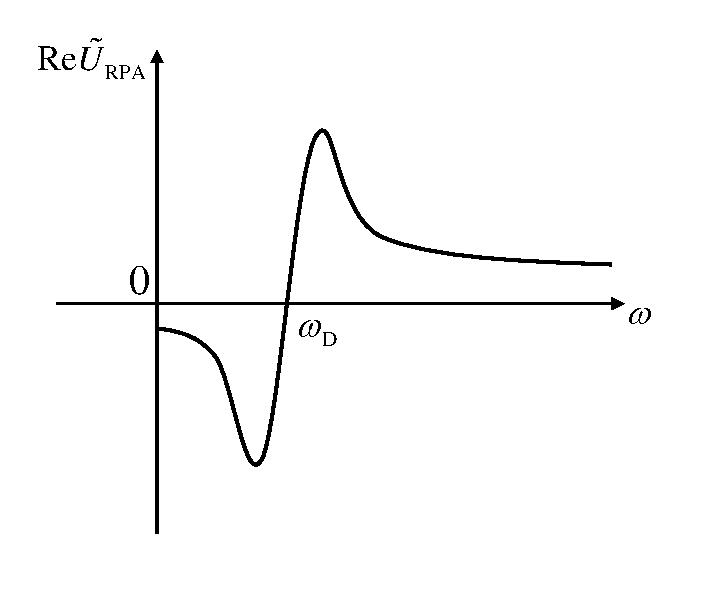
\includegraphics[width=7cm]{figure/RPA1.pdf}
    \caption{有效相互作用势实部随频率变化曲线.}
    \label{U-rpa}
\end{figure}

\subsection{电子-声子系统有效哈密顿量}

前面已经基本分析完了金属体系中, 声子对电子系统的影响. 现在我们要考虑电子-声子相互作用对电子态的影响. 在这里我们不需要从头开始重新计算, 只要选取能突出基本物理的有效哈密顿量即可, 这就是这里讨论有效哈密顿量的原因. 电子-声子系统的有效哈密顿量由三部分组成: 
\begin{equation}
    \hat{H}_{\fun{eff}}=\hat{H}_{\fun{el}}+\hat{H}_{\fun{ph}}+\hat{H}_{\fun{el-ph}},
\end{equation}
其中: 
\begin{equation}
    \hat{H}_{\fun{el}}=\sum_{k\sigma}\ls \frac{k^2\hbar^2}{2m^*}-\mu \rs \hat{c}_{k\sigma}^{\dg}\hat{c}_{k\sigma}^{ },
\end{equation}
\begin{equation}
    \hat{H}_{\fun{ph}}=\sum_q\tilde{\omega}(\vct{q})\ls \hat{a}_q^\dg \hat{a}_q^{ }+\frac{1}{2} \rs,
\end{equation}
\begin{equation}
    \hat{H}_{\fun{el-ph}}=\sum_{k\sigma}\sum_{q\ne 0}g_{\fun{RPA}}(\vct{q})\hat{A}_q^{ }\hat{c}_{k+q,\sigma}^\dg \hat{c}_{k\sigma}^{ },
\end{equation}
考虑进声子相互作用后, 每个子系统哈密顿量都不同于原始哈密顿量. 其中 $\hat{c}_{k\sigma}^\dg$ 和 $\hat{c}_{k\sigma}^{ }$ 是有效电子的产生湮灭算符, 声子频率 $\tilde{\omega}(\vct{q})$ 是前面我们修正过的, 电声耦合 $g_{\fun{RPA}}(\vct{q})$ 也是前面修正过后的结果.

不考虑电子-电子相互作用, 电子自能和声子自能可以分别用费曼图表示为 
$$
    \feyndiagram{
        \vertex[NWblob](a)at(1,0){};
        \vertex[NWblob](b)at(-1,0){};
        \propag[plain](2,0)to(a);
        \propag[plain](a)to(b);
        \propag[plain](b)to(-2,0);
        \propag[bos](a)to[half right, looseness=1.6](b);
        \vertex(c)at(0,0.8){$D_{\fun{RPA}}$};
        \vertex(d)at(0,-1.3){电子自能};
    },\qquad\quad
    \feyndiagram{
        \vertex[NWblob](a)at(0.7,0){};
        \vertex[NWblob](b)at(-0.7,0){};
        \propag[bos](2,0)to(a);
        \propag[plain](a)to[half left, looseness=1.4](b);
        \propag[plain](b)to[half left, looseness=1.4](a);
        \propag[bos](b)to(-2,0);
        \vertex(c)at(1.7,0.4){$D_{\fun{RPA}}$};
        \vertex(c)at(-1.7,0.4){$D_{\fun{RPA}}$};
        \vertex(d)at(0,-1.3){声子自能};
    }.
$$
上述两个修正过的自能图可以用于讨论电子-声子相互作用对金属电阻随温度变化的影响. 

另外, 可以由 Migdal 定理证明关系式: 
\begin{equation}
    \feyndiagram{
        \vertex[NWblob](a)at(0,0){};
        \vertex[NWblob](b)at(-1,-1){};
        \vertex[NWblob](c)at(-1,1){};
        \propag[bos](1.5,0)to(a);
        \propag[plain](a)to(b);
        \propag[plain](a)to(c);
        \propag[plain](b)to(-2,-2);
        \propag[plain](c)to(-2,2);
        \propag[bos](b)to[half left, looseness=1.6](c);
    }
    \propto 
    \sqrt{\frac{m}{M}}\times
    \feyndiagram{
        \vertex[NWblob](a)at(0,0){};
        \propag[bos](1.5,0)to(a);
        \propag[plain](a)to(-1,-1);
        \propag[plain](a)to(-1,1);
    },
\end{equation}
Migdal 这一证明的前提假设也是 $\tilde{\omega_q}\propto c_{\fun{L}}q$, 因此整体来说, 我们在上面给出的推导是自洽的.

\section{Gor'kov 的超导格林函数理论(松原格林函数的应用之三)}
正确的超导理论最早是 1956 年提出的 BCS 理论, 这一套理论虽然成功, 但是它的短板是只能考虑大块的均匀超导体. 当系统具有外磁场等影响时, 这套理论将束手无策. 因此我们非常需要一套能够处理非均匀情况的超导理论. Gor'kov 于 1958 年提出的格林函数的超导理论正是用来描述非均匀超导的一套成功的理论, 其中运用的就是有限温的格林函数. 

在 1950 年左右, 人们提出了一套超导的唯象理论, 即 G-L 理论, 但这一理论的微观基础人们并不明确. Gor'kov 理论从微观的格林函数满足的方程出发, 导出了 G-L 理论满足的方程. 这一做法非常令人惊叹, 这一套理论需要大量推导. 可见 Gor'kov 的物理直觉十分敏锐, 数学功底非常扎实. 希望理论工作的同学们要向老一辈物理学家看齐, 学习他们认真踏实, 坚韧不拔, 严密的工作精神. 

下面我们简单地介绍一下这一理论. 
\subsection{约化哈密顿量及其平均场近似}
约化哈密顿量由两部分构成:
\begin{equation}
    \hat{H}=\hat{H}_0+\hat{H}',\quad \hat{H}_0=\sum_\alpha \int\dd \vct{x}\hat{\psi}_\alpha^{\dg}(\vct{x})\hat{h}(\vct{x})\hat{\psi}_\alpha^{ }(\vct{x}),
\end{equation}
其中 $\hat{h}(\vct{x})$ 是单体算符, 表示为 
\begin{equation}
    \hat{h}(\vct{x})=\frac{\lmi -\ii\nabla-e\vct{A}(\vct{x}) \rmi^2}{2m},
\end{equation}
其中 $\hat{A}(\vct{x})$ 是磁矢势. 在这里还考虑了 London 规范, 即有 
\begin{equation}
    \left\{
        \begin{aligned}
            &\nabla\times\vct{A}=\vct{B},\\
            &\nabla\cdot\vct{A}=0.
        \end{aligned}
    \right.
\end{equation}
在巨正则系综下有 
\begin{equation}
    \hat{h}_\mu(\vct{x})=\hat{h}(\vct{x})-\mu.
\end{equation}

二体相互作用项表示为 
\begin{equation}
    \hat{H}'=\frac{1}{2}\sum_{\alpha\beta}\iint\dd\vct{x}\dd \vct{x}'\hat{\psi}_\alpha^\dg (\vct{x})\hat{\psi}_{\beta}^\dg(\vct{x}')V(\vct{x}-\vct{x}')\hat{\psi}_{\beta}^{ }(\vct{x}')\hat{\psi}_{\alpha}^{ }(\vct{x}).
\end{equation}
这里的相互作用势对超导体来说 $V<0$ 是吸引势. 为简单起见, 我们考虑以下几种简化情况.

(a) 自旋单态超导体 

自旋单态超导体的自旋指标 $\beta=\bar{\alpha}$, 即二体相互作用项可以简化为 
  \begin{align}
        \hat{H}'=&\frac{1}{2}\sum_{\alpha}\iint\dd\vct{x}\dd \vct{x}'\hat{\psi}_\alpha^\dg (\vct{x})\hat{\psi}_{\bar{\alpha}}^\dg(\vct{x}')V(\vct{x}-\vct{x}')\hat{\psi}_{\bar{\alpha}}^{ }(\vct{x}')\hat{\psi}_{\alpha}^{ }(\vct{x})\nonumber\\
        =&\iint\dd\vct{x}\dd\vct{x}'\hat\psi_{\ua}^\dg(\vct{x})\hat\psi_\da^\dg(\vct{x}')V(\vct{x}-\vct{x}')\hat\psi_\da^{ }(\vct{x}')\hat\psi_\ua^{ }(\vct{x}).
    \end{align}

(b) 只考虑 $s$-波情况 

此时只有点接触型相互作用 $V(\vct{x}-\vct{x}')=-g\delta(\vct{x}-\vct{x}')$, 其中 $g>0$. 此时二体相互作用项写为  
\begin{equation}
    \hat{H}'=-g\int\dd\vct{x}\hat{\psi}_\ua^\dg(\vct{x})\hat\psi_\da^\dg(\vct{x})\hat{\psi}_\da^{ }(\vct{x})\hat{\psi}_{\ua}^{ }(\vct{x}),
\end{equation}
这样的场算符四次项难以处理, 下面我们取平均场近似进行计算.

平均场近似的基本假设是 
\begin{equation}
    \llag \hat{\psi}_\ua^\dg(\vct{x})\hat\psi_\da^\dg(\vct{x}) \rrag\ne 0,\quad \llag \hat\psi_\da(\vct{x})\hat\psi_\ua(\vct{x}) \rrag\ne 0.
\end{equation}
将场算符二次项表示为 
\begin{equation}
    \hat{\psi}_{\downarrow}(\vct{x}) \hat{\psi}_{\uparrow}(\vct{x})=\left\langle\hat{\psi}_{\downarrow}(\vct{x}) \hat{\psi}_{\uparrow}(\vct{x})\right\rangle+\left(\hat{\psi}_{\downarrow}(\vct{x}) \hat{\psi}_{\uparrow}(\vct{x})-\left\langle\hat{\psi}_{\downarrow}(\vct{x}) \hat{\psi}_{\uparrow}(\vct{x})\right\rangle\right),
\end{equation}
\begin{equation}
    \hat{\psi}_{\uparrow}^\dg(\vct{x}) \hat{\psi}_{\downarrow}^\dg(\vct{x}) =\left\langle\hat{\psi}_{\uparrow}^\dg(\vct{x}) \hat{\psi}_{\downarrow}^\dg(\vct{x})\right\rangle+\left(\hat{\psi}_{\uparrow}^\dg(\vct{x}) \hat{\psi}_{\downarrow}^\dg(\vct{x})-\left\langle\hat{\psi}_{\uparrow}^\dg(\vct{x}) \hat{\psi}_{\downarrow}^\dg(\vct{x})\right\rangle\right) .
\end{equation}
将括号中的两项视为一阶涨落 $\delta$, 并忽略二阶及以上的小量, 二体相互作用项可以表示为
 \begin{align}
        \hat{H}'= & -g \int \mathrm{d} \vct{x}\left[\left\langle\hat{\psi}_{\uparrow}^\dg(\vct{x}) \hat{\psi}_{\downarrow}^\dg(\vct{x})\right\rangle+\left(\hat{\psi}_{\uparrow}^\dg(\vct{x}) \hat{\psi}_{\downarrow}^\dg(\vct{x})-\left\langle\hat{\psi}_{\uparrow}^\dg(\vct{x}) \hat{\psi}_{\downarrow}^\dg(\vct{x})\right\rangle\right)\right]\nonumber \\
        & \times{\left[\left\langle\hat{\psi}_{\downarrow}(\vct{x}) \hat{\psi}_{\uparrow}(\vct{x})\right\rangle+\left(\hat{\psi}_{\downarrow}(\vct{x}) \hat{\psi}_{\uparrow}(\vct{x})-\left\langle\hat{\psi}_{\downarrow}(\vct{x}) \hat{\psi}_{\uparrow}(\vct{x})\right\rangle\right)\right] } \nonumber\\
        \approx & -g \int \mathrm{d} \vct{x}\left(\left\langle\hat{\psi}_{\uparrow}^\dg(\vct{x}) \hat{\psi}_{\downarrow}^\dg(\vct{x})\right\rangle \hat{\psi}_{\downarrow}(\vct{x}) \hat{\psi}_{\uparrow}(\vct{x})+\hat{\psi}_{\uparrow}^\dg(\vct{x}) \hat{\psi}_{\downarrow}^\dg(\vct{x})\left\langle\hat{\psi}_{\downarrow}(\vct{x}) \hat{\psi}_{\uparrow}(\vct{x})\right\rangle\right.\nonumber\\
        &\qquad\qquad\left.-\left\langle\hat{\psi}_{\uparrow}^\dg(\vct{x}) \hat{\psi}_{\downarrow}^\dg(\vct{x})\right\rangle\left\langle\hat{\psi}_{\downarrow}(\vct{x}) \hat{\psi}_{\uparrow}(\vct{x})\right\rangle\right),
        \end{align}
定义\textbf{对势}(\textbf{pair potential}) $\Delta$:
\begin{equation}
    \left\{
        \begin{aligned}
            &-g\left\langle\hat{\psi}_{\downarrow}(\vct{x}) \hat{\psi}_{\uparrow}(\vct{x})\right\rangle \equiv \Delta(\vct{x}), \\
            &-g\left\langle\hat{\psi}_{\uparrow}^\dg(\vct{x}) \hat{\psi}_{\downarrow}^\dg(\vct{x})\right\rangle \equiv \Delta^*(\vct{x}) ,
        \end{aligned}
    \right.
\end{equation}
通常也称 $\Delta$ 为能隙函数, 此处要注意它不是一个算符. 

这样就可以把平均场哈密顿量表示为
  \begin{align}
        \hat{H}=&\sum_\alpha \int \mathrm{d} \vct{x} \hat{\psi}_\alpha^\dg(\vct{x}) \hat{h}_\mu(\vct{x}) \hat{\psi}_\alpha(\vct{x})+\int \mathrm{d} \vct{x} \Delta^*(\vct{x}) \hat{\psi}_{\downarrow}(\vct{x}) \hat{\psi}_{\uparrow}(\vct{x})\nonumber\\
        &+\int \mathrm{d} \vct{x} \Delta(\vct{x}) \hat{\psi}_{\uparrow}^\dg(\vct{x}) \hat{\psi}_{\downarrow}^\dg(\vct{x})+\int \mathrm{d} \vct{x} \frac{|\Delta(\vct{x})|^2}{g}.
    \end{align}
\subsection{Gor'kov 的超导格林函数}
为求解平均场近似下的哈密顿量, 定义如下单粒子松原格林函数: 
\begin{equation}
    \mathcal{G}_{\alpha\beta}(\vct{x},\tau;\vct{x}',\tau')=-\llag \hat{T}_\tau\lmi \hat{\psi}_{H\alpha}^{ }(\vct{x},\tau)\hat{\psi}_{H\beta}^\dg(\vct{x}',\tau') \rmi \rrag,
\end{equation}
其中场算符是有限温下的海森堡算符: 
\begin{equation}
    \left\{
        \begin{aligned}
            &\hat{\psi}_{H\alpha}^{ }(\vct{x},\tau)=\e^{\hat{K}\tau}\hat\psi_{\alpha}^{ }(\vct{x})\e^{-\hat{K}\tau},\\
            &\hat{\psi}_{H\beta}^{\dg}(\vct{x}',\tau')=\e^{\hat{K}\tau'}\hat{\psi}_{\beta}^{\dg}(\vct{x}')\e^{-\hat{K}\tau'}.
        \end{aligned}
    \right.
\end{equation}
另外, 此处 $\lag\cdots\rag$ 定义为 
\begin{equation}
    \lag\cdots\rag\equiv \frac{\fun{Tr}\lmi \e^{-\beta\hat{K}}\cdots \rmi}{\fun{Tr}\lmi \e^{-\beta\hat{K}} \rmi}.
\end{equation}

超导的核心思想之一在于费米面附近的态密度足够大, 总可以把任意的色散关系在费米面附近线性展开, 这样就和光子的色散关系一致了, 也就是有化学势 $\mu=0$, 粒子数任意变化而不会改变能量. 所以有巨正则系综下的 $\hat{K}\equiv \hat{H}$. 

下面我们分别用运动方程法和有限温下的费曼图技术求解这一单粒子松原格林函数, 导出 Gor'kov 方程.
\subsection{海森伯绘景中的解法(运动方程法)}
首先考虑场算符的时间导数 
 \begin{align}
        \frac{\pt}{\pt\tau}\hat{\psi}_{H\alpha}(\vct{x},\tau)=&\ls\frac{\pt}{\pt\tau}\e^{\hat{K}\tau}\rs \hat{\psi}_{\alpha}(\vct{x})\e^{-\hat{K}\tau}+\e^{\hat{K}\tau}\hat{\psi}_{\alpha}(\vct{x})\ls \frac{\pt}{\pt \tau}\e^{-\hat{K}\tau} \rs\nonumber\\
        =&\hat{K}\e^{\hat{K}\tau}\hat{\psi}_{\alpha}(\vct{x})\e^{-\hat{K}\tau}-\e^{\hat{K}\tau}\hat{\psi}_{\alpha} (\vct{x})\e^{-\hat{K}\tau}\hat{K}\nonumber\\
        =&\lmi \hat{K},\hat{\psi}_{H\alpha}(\vct{x},\tau) \rmi_-,
    \end{align}
代入超导哈密顿量 $\hat{H}$ 的具体表达式并计算对易关系, 有: 
\begin{align}
        \lmi \hat{H},\hat{\psi}_{\alpha}(\vct{x}) \rmi_-=&\sum_{\beta}\int\dd\vct{x}'\lmi \hat{\psi}_{\beta}^\dg(\vct{x}')\hat{h}(\vct{x}')\hat{\psi}_{\beta}^{ }(\vct{x}'),\hat{\psi}_{\alpha}^{ }(\vct{x}) \rmi_- \nonumber\\
&+ \int\dd\vct{x}'\lmi \Delta(\vct{x}')\hat{\psi}_{\alpha}^\dg (\vct{x}')\hat{\psi}_{\bar{\alpha}}^\dg (\vct{x}'),\hat{\psi}_\alpha^{ }(\vct{x}) \rmi_-,
    \end{align}
第一项对易式: 
 \begin{align}
      \sum_{\beta}\int\dd\vct{x}'  \lmi \hat{\psi}_{\beta}^\dg(\vct{x}')\hat{h}(\vct{x}')\hat{\psi}_{\beta}^{ }(\vct{x}'),\hat{\psi}_{\alpha}(\vct{x}) \rmi_-=&\sum_{\beta}\int\dd\vct{x}'\lmi \hat{\psi}_{\beta}^\dg(\vct{x}'),\hat{\psi}_\alpha(\vct{x}) \rmi_- \hat{h}(\vct{x}')\hat{\psi}_\beta^{ }(\vct{x}')\nonumber\\
        =&-\sum_{\beta}\int\dd\vct{x}'\delta_{\alpha\beta}\delta(\vct{x}'-\vct{x})\hat{h}(\vct{x}')\hat{\psi}_{\beta}^{ }(\vct{x}')\nonumber\\
        =&-\hat{h}(\vct{x})\hat{\psi}_{\alpha}^{ }(\vct{x}),
    \end{align}
第二项对易式
 \begin{align}
       \int\dd\vct{x}' \lmi \Delta(\vct{x}')\hat{\psi}_{\alpha}^\dg(\vct{x}')\hat{\psi}_{\bar{\alpha}}^\dg (\vct{x}'), \hat{\psi}_{\alpha}^{ }(\vct{x})\rmi_-=&-\int\dd\vct{x}'\Delta(\vct{x}')\hat{\psi}_{\bar{\alpha}}^\dg(\vct{x}')\ls -\delta(\vct{x}'-\vct{x}) \rs\nonumber\\
        =&-\Delta(\vct{x})\hat{\psi}_{\bar{\alpha}}^\dg(\vct{x}),
    \end{align}
所以有 
\begin{equation}
    \frac{\pt}{\pt\tau}\hat{\psi}_{H\alpha}^{ }(\vct{x},\tau)=-\hat{h}(\vct{x})\hat{\psi}_{H\alpha}^{ }(\vct{x},\tau)-\alpha\Delta(\vct{x})\hat{\psi}_{H\bar{\alpha}}^\dg(\vct{x},\tau).
\end{equation}
类似地, 有
\begin{equation}
    \frac{\pt}{\pt\tau}\hat{\psi}_{H\alpha}^\dg (\vct{x},\tau)=\hat{h}(\vct{x})\hat{\psi}_{H\alpha}^\dg (\vct{x},\tau)+\alpha\Delta^*(\vct{x})\hat{\psi}_{H\bar\alpha}^{ }(\vct{x},\tau).
\end{equation}
格林函数对"时间"的导数就可以写成: 
  \begin{align}
        \frac{\pt}{\pt \tau}\mathcal{G}_{\alpha\alpha}(\vct{x},\tau;\vct{x}',\tau')=&-\delta(\vct{x}-\vct{x}')\delta(\tau-\tau')-\hat{h}(\vct{x})\mathcal{G}_{\alpha\alpha}(\vct{x},\tau;\vct{x}',\tau')\nonumber\\
&+\alpha \Delta(\vct{x})\mathcal{F}_{\bar{\alpha}\alpha}^{\dg}(\vct{x},\tau;\vct{x}',\tau'),
    \end{align}
其中定义了反常格林函数 
\begin{equation}
    \mathcal{F}_{\bar{\alpha}\alpha}^\dg\equiv \llag \hat{T}_\tau \lmi \hat{\psi}_{H\bar \alpha}^\dg(\vct{x},\tau)\hat{\psi}_{H\alpha}^\dg(\vct{x}',\tau') \rmi \rrag,
\end{equation}
其中改变了自旋指标, 这并不影响计算结果. 这一项在正常态费米子体系中等于零, 但在超导体系中可以不等于零. 另外, 反常格林函数与超导能隙函数直接相关, 即有 
\begin{equation}
    \mathcal{F}_{\downarrow\uparrow}^\dg(\vct{x},\tau;\vct{x}',\tau')=\frac{\Delta^*(\vct{x})}{g}.
\end{equation}

下面求解关于 $\mathcal{F}_{\alpha\beta}^\dg$ 的运动方程, 对 $\tau$ 求导有 
\begin{equation}
    \frac{\pt}{\pt\tau}\mathcal{F}_{\bar{\alpha}\alpha}^\dg(\vct{x},\tau;\vct{x}',\tau')=\hat{h}^*(\vct{x})\mathcal{F}_{\bar{\alpha}\alpha}^\dg(\vct{x},\tau;\vct{x}',\tau')+\alpha \Delta^*(\vct{x})\mathcal{G}_{\alpha\alpha}(\vct{x},\tau;\vct{x}',\tau').
\end{equation}
与前面对 $\mathcal{G}_{\alpha\alpha}$ 的时间导数联立, 得到 Gor'kov 方程组:
\begin{equation}
    \left\{
        \begin{aligned}
            &\frac{\pt}{\pt\tau}\mathcal{G}(\vct{x},\tau;\vct{x}',\tau')=-\delta(\vct{x}-\vct{x}')\delta(\tau-\tau')-\hat{h}(\vct{x})\mathcal{G}(\vct{x},\tau;\vct{x}',\tau')+\Delta(\vct{x})\mathcal{F}^\dg(\vct{x},\tau;\vct{x}',\tau'),\\
            &\frac{\pt}{\pt\tau}\mathcal{F}^\dg(\vct{x},\tau;\vct{x}',\tau')=\hat{h}^*(\vct{x})\mathcal{F}^\dg(\vct{x},\tau;\vct{x}',\tau')+\Delta^*(\vct{x})\mathcal{G}(\vct{x},\tau;\vct{x}',\tau').
        \end{aligned}
    \right.
\end{equation}
由于这里的哈密顿量与时间无关, 可以对时间进行傅立叶变换, 得到:
\begin{equation}
    \left\{
    \begin{aligned}
        &\lmi \ii\omega_n-\hat h(\vct{x}) \rmi\mathcal{G}(\vct{x},\vct{x}';\ii\omega_n)+\Delta(\vct{x})\mathcal{F}^\dg (\vct{x},\vct{x}';\ii\omega_n)=\delta(\vct{x}-\vct{x}'),\\
        &\lmi \ii\omega_n+\hat h^*(\vct{x}) \rmi \mathcal{F}^\dg(\vct{x},\vct{x}';\ii\omega_n)+\Delta^*(\vct{x})\mathcal{G}(\vct{x},\vct{x}';\ii\omega_n)=0,
    \end{aligned}
    \right. 
\end{equation}
同样是 Gor'kov 方程.

在无外磁场的情况下, 系统是空间均匀的, 此时哈密顿量只是粒子坐标差的函数. 因此能隙函数 $\Delta$ 成为一个与坐标无关的常数. 方程可以进一步写成 
\begin{equation}
    \left\{
        \begin{aligned}
            &\lmi \ii\omega_n-\xi_k \rmi\mathcal{G}(\vct{k},\ii\omega_n)+\Delta\mathcal{F}^\dg (\vct{k},\ii\omega_n)=\vct{1},\\
            &\lmi \ii\omega_n +\xi_k\rmi\mathcal{F}^\dg (\vct{k},\ii\omega_n)+\Delta^*\mathcal{G}(\vct{k},\ii\omega_n)=0,
        \end{aligned}
    \right.
\end{equation}
其中有 
\begin{equation}
    \xi_k=\frac{\hbar^2 k^2}{2m}-\mu\equiv \epsilon_k^0-\mu.
\end{equation}
从方程组中易解出 
\begin{equation}
    \left\{
        \begin{aligned}
            &\mathcal{G}(\vct{k},\ii\omega_n)=-\frac{\ii\omega_n+\xi_k}{\omega_n^2+E_k^2},\\
            &\mathcal{F}^\dg(\vct{k},\ii\omega_n)=\frac{\Delta^*}{\omega_n^2+E_k^2},
        \end{aligned}
    \right.
\end{equation}
其中: 
\begin{equation}
    E_k^2\equiv \xi_k^2+|\Delta|^2.
\end{equation}
下一小节利用费曼图技术重新推导出这一结果.
\subsection{费曼图法}
考虑相互作用绘景下的松原格林函数及各自的费曼图:
\begin{equation}
    \left\{
        \begin{aligned}
            &\mathcal{G}_{\ua\da}(\vct{x},\tau;\vct{x}',\tau')=-\llag\hat{T}_{\tau}\lmi \hat{\psi}_{I\ua}(\vct{x},\tau)\hat{\psi}_{I\ua}^\dg(\vct{x}',\tau')\hat{S}(\beta,0) \rmi \rrag_{0\fun{C}}:&\feyndiagram{\propag[doublefermion](1,0)to(-1,0);},\\
            &\mathcal{F}_{\da\ua}^\dg (\vct{x},\tau;\vct{x}',\tau')=\llag \hat{T}_\tau\lmi \hat{\psi}_{I\da}^\dg(\vct{x},\tau)\hat{\psi}_{I\ua}^\dg(\vct{x}',\tau')\hat{S}(\beta,0) \rmi \rrag_{0\fun{C}}:&\feyndiagram{\propag[doublefermion](1,0)to(0,0);\propag[doublefermion](-1,0)to(0,0);}.
        \end{aligned}
    \right.
\end{equation}
其中相互作用绘景下的场算符表达式为 
\begin{equation}
    \hat{\psi}_{I\da}^\dg(\vct{x},\tau)=\e^{\hat{H}_0\tau}\hat{\psi}_{\da}^\dg(\vct{x})\e^{-\hat{H}_0\tau},
\end{equation}
有限温下的散射矩阵 $\hat{S}$ 表达式为
\begin{equation}
    \hat{S}(\beta,0)=\hat{T}_\tau\fun{exp}\lmi -\int_0^\beta\hat{H}_I'(\tau')\dd\tau' \rmi,
\end{equation} 
这一项的展开式从二阶项开始.

用单费米线 $\feyndiagram{\propag[fer](0.5,0)to(-0.5,0);}$ 表示自由粒子系统格林函数 $\mathcal{G}^{0}(\vct{x},\tau;\vct{x}',\tau')$, 格林函数的展开式就可以表示为 
   \begin{align}
        \feyndiagram{
            \propag[doublefermion](1,0)to(-1,0);
            \vertex(a)at(0,-0.4){$\vct{k},\ii\omega_n$};
        }
        =\; 
        &
        \feyndiagram{
            \propag[fer](1,0)to(-1,0);
            \vertex(a)at(0,-0.4){$\vct{k},\ii\omega_n$};
        }
        +
        \feyndiagram{
            \propag[fer](-1,0)to(-3,0);
            \propag[fer](-1,0)to(1,0);
            \propag[fer](3,0)to(1,0);
            \propag[sca](-1,0)to(-1,1);
            \propag[sca](1,0)to(1,1);
            \vertex(a)at(1.1,1.1){$\Delta^*$};
            \vertex(b)at(-1,1.1){$\Delta$};
            \vertex(c)at(-2.3,-0.3){$\vct{k},\ii\omega_n$};
            \vertex(d)at(0,-0.3){$ -\vct{k},-\ii\omega_n$};
            \vertex(e)at(2.3,-0.3){$\vct{k},\ii\omega_n$};
        }\nonumber\\
        &+
        \feyndiagram{
            \propag[fer](-3,0)to(-1,0);
            \propag[fer](1,0)to(-1,0);
            \propag[fer](1,0)to(3,0);
            \propag[fer](5,0)to(3,0);
            \propag[fer](-3,0)to(-5,0);
            \propag[sca](-1,0)to(-1,1);
            \propag[sca](1,0)to(1,1);
            \propag[sca](-3,0)to(-3,1);
            \propag[sca](3,0)to(3,1);
            \vertex(a)at(1,1.1){$\Delta$};
            \vertex(b)at(-0.9,1.1){$\Delta^*$};
            \vertex(f)at(-3,1.1){$\Delta$};
            \vertex(g)at(3.1,1.1){$\Delta^*$};
        }\nonumber\\
        &+\cdots,
    \end{align}
回顾前面章节中, 我们用正规自能表示格林函数时有
 \begin{align}
        \feyndiagram{\propag[doublefermion] (0.4,0) to (-0.5,0);}=\; &
        \feyndiagram{\propag[fer] (0.4,0) to (-0.4,0);}
        +
        \feyndiagram{\vertex (a) at (-1,0);\selfnormalsigma{b}{0,0};\vertex (c) at (1,0);\propag[fer](b) to (a);\propag[fer] (c) to (b);}
        +
        \feyndiagram{\vertex (a) at (-1.5,0);\selfnormalsigma{b}{-0.5,0};\selfnormalsigma{c}{0.5,0};\vertex (d) at (1.5,0);\propag[fer] (b) to (a);\propag[plain](c) to (b);\propag[fer](d) to (c);}
        % +
        % \feyndiagram{\vertex (a) at (-1.5,0);\selfnormalsigma{b}{-0.5,0};\selfnormalsigma{c}{0.5,0};\selfnormalsigma{d}{1.5,0};\vertex (e) at (2.5,0);\propag[fer] (b) to (a);\propag[plain](c) to (b);\propag[plain](d) to (c);\propag[fer] (e) to (d);}
        +\cdots\nonumber\\
        =&\feyndiagram{\propag[fer] (0.4,0) to (-0.4,0);}
         +
            \feyndiagram{
            \vertex(a)at(-1,0);
            \selfnormalsigma{b}{0,0};
            \vertex(c)at(1,0);
            \propag[fer](b)to(a);
            \propag[doublefermion](c)to(b);
        },
    \end{align}
可以按照类似的关系来定义超导格林函数的正规自能:
\begin{equation}
    \feyndiagram{
        \propag[fer](-1,0)to(1,0);
        \propag[sca](-1,0)to(-1,1);
        \propag[sca](1,0)to(1,1);
        \vertex(a)at(-1,1.1){$\Delta$};
        \vertex(b)at(1.1,1.1){$\Delta^*$};
    },\quad\Sigma^*\equiv-\frac{|\Delta|^2}{-\ii\omega_n-\xi_{-k}}=\frac{|\Delta|^2}{\ii\omega_n+\xi_k},
\end{equation}
从而得到格林函数 
\begin{equation}
    \mathcal{G}(\vct{k},\ii\omega_n)=\frac{1}{\ii\omega_n-\xi_k-\frac{|\Delta|^2}{\ii\omega_n+\xi_k}}=-\frac{\ii\omega_n+\xi_k}{\omega_n^2+E_k^2},
\end{equation}
这一结果与前一节的计算结果一致. 

类似地, 有反常格林函数的费曼图展开式 
  \begin{align}
        \feyndiagram{
            \propag[doublefermion](1,0)to(0,0);
            \propag[doublefermion](-1,0)to(0,0);
            }
            =\;&
            \feyndiagram{
                \propag[fer](-1,0)to(0,0);
                \propag[fer](1,0)to(0,0);
                \propag[sca](0,0)to(0,1);
                \vertex(a)at(0.1,1.1){$\Delta^*$};
            }
            +
            \feyndiagram{
                \propag[fer](-2,0)to(-1,0);
                \propag[fer](0,0)to(-1,0);
                \propag[fer](0,0)to(1,0);
                \propag[fer](2,0)to(1,0);
                \propag[sca](-1,0)to(-1,1);
                \propag[sca](0,0)to(0,1);
                \propag[sca](1,0)to(1,1);
                \vertex(a)at(-0.9,1.1){$\Delta^*$};
                \vertex(b)at(0,1.1){$\Delta$};
                \vertex(c)at(1.1,1.1){$\Delta^*$};
            }
            +\cdots\nonumber\\
            =\;&
            \feyndiagram{
                \propag[fer](-1,0)to(0,0);
                \propag[doublefermion](1,0)to(0,0);
                \propag[sca](0,0)to(0,1);
                \vertex(a)at(0.1,1.1){$\Delta^*$};
            },
    \end{align}
解出反常格林函数为 
\begin{equation}
    \mathcal{F}^\dg(\vct{k},\ii\omega_n)=\frac{\Delta^*}{-\ii\omega_n-\xi_k}\ls -\frac{\ii\omega_n+\xi_k}{\omega_n^2+E_k^2} \rs=\frac{\Delta^*}{\omega_n^2+E_k^2}.
\end{equation}

费曼图形式的方程组:
\begin{equation}
    \left\{
    \begin{aligned}
        &\feyndiagram{
            \propag[doublefermion](0.6,0)to(-0.6,0);
        }
        =\;
        \feyndiagram{
            \propag[fer](1,0)to(-1,0);
        }
        +
        \feyndiagram{
            \propag[fer](0,0)to(-1,0);
            \propag[doublefermion](1.2,0)to(0.6,0);
            \propag[doublefermion](0,0)to(0.6,0);
            \propag[sca](0,0)to(0,1);
            \vertex(a)at(0.1,1.1){$\Delta^*$};
        },\\
        &\feyndiagram{
            \propag[doublefermion](-0.6,0)to(0,0);
            \propag[doublefermion](0.6,0)to(0,0);
        }
        =
        \feyndiagram{
            \propag[fer](-1,0)to(0,0);
            \propag[doublefermion](1,0)to(0,0);
            \propag[sca](0,0)to(0,1);
            \vertex(a)at(0.1,1.1){$\Delta^*$};
        },
    \end{aligned}
    \right.
\end{equation}
亦即 Gor'kov 方程.

对超导格林函数变形:
 \begin{align}
        \mathcal{G}(\vct{k},\ii\omega_n)&=-\frac{\ii\omega_n+\xi_k}{\omega_n^2+E_k^2}\nonumber\\
        &=\frac{u_k^2}{\ii\omega_n-E_k}+\frac{v_k^2}{\ii\omega_n+E_k}\nonumber\\
        &\equiv \int_{-\infty}^{\infty}\frac{A(\vct k,\omega')}{\ii\omega_n-\omega'}\dd\omega',
    \end{align}
其中有 
\begin{equation}
    \left\{
        \begin{aligned}
            &u_k^2=\frac{1}{2}\left( 1+\frac{\xi_k}{E_k} \right),\\
            &v_k^2=\frac{1}{2}\left( 1-\frac{\xi_k}{E_k} \right),
        \end{aligned}
    \right.
\end{equation}
并且有关系式 $u_k^2+v_k^2=1$. 另外, 谱函数 $A(\vct{k},\omega)$ 的表达式为 
\begin{equation}
    A(\vct{k},\omega)=u_k^2\delta(\omega-E_k)+v_k^2\delta(\omega+E_k),
\end{equation}
格林函数的正极点对应着准粒子的能量, 有 
\begin{equation}
    E_k=\sqrt{\xi_k^2+|\Delta|^2},
\end{equation}
其中有
\begin{equation}
    \xi_k=\frac{k^2}{2m}-E_{\fun{F}},
\end{equation}
当 $k=k_{\fun{F}}$ 时上式取最小值, 在 $\mu=E_{\fun{F}}$ 时这一结果符合弱耦合理论. 这时 $E_k=|\Delta|$ 称为能隙, 即激发准粒子需要的最小能量.

反常格林函数也可以表示为 
  \begin{align}
        \mathcal{F}^\dg(\vct{k},\ii\omega_n)=&\frac{\Delta^*}{\omega_n^2+E_k^2}\nonumber\\
        =&-\frac{\Delta^*}{2E_k}\ls \frac{1}{\ii\omega_n-E_k}-\frac{1}{\ii\omega_n+E_k} \rs,
    \end{align}
\subsection{物理量的计算}
(a) 能隙方程 

对于大块的超导体, 我们可以选取 $\Delta$ 为实数, 能隙函数可以表示为 
\begin{equation}
    \Delta^*=g\mathcal{F}^\dg(0,-\eta),
\end{equation}
考虑反常格林函数的傅立叶变换 
\begin{equation}
    \mathcal{F}^\dg(\vct{x}-\vct{x}';\tau-\tau')=\int\frac{\dd\vct
    k}{(2\pi)^3}\frac{1}{\beta}\sum_{\omega_n}\e^{\ii\vct{k}\cdot(\vct{x}-\vct{x}')}\e^{-\ii\omega_n(\tau-\tau')}\mathcal{F}^\dg(\vct{k},\ii\omega_n),
\end{equation}
取 $\tau'=\tau+\eta$, $\vct{x}'=\vct{x}$, 就有 
\begin{equation}
    \mathcal{F}^\dg(0,-\eta)=\int\frac{\dd\vct
    k}{(2\pi)^3}\frac{1}{\beta}\sum_{\omega_n}\e^{\ii\omega_n\eta}\mathcal{F}^\dg(\vct{k},\ii\omega_n).
\end{equation}
能隙函数就可以表示成 
  \begin{align}
        \Delta^*&=g\int\frac{\dd\vct
        k}{(2\pi)^3}\frac{1}{\beta}\sum_{\omega_n}\e^{\ii\omega_n\eta}\lmi -\frac{\Delta^*}{2E_k}\ls \frac{1}{\ii\omega_n-E_k}-\frac{1}{\ii\omega_n+E_k} \rs \rmi\nonumber\\
        &=-g\int\frac{\dd\vct{k}}{(2\pi)^3}\ls \frac{1}{\beta}\sum_{\omega_n}\frac{\e^{\ii\omega_n\eta}}{\ii\omega_n-E_k}-\frac{1}{\beta}\sum_{\omega_n}\frac{\e^{\ii\omega_n\eta}}{\ii\omega_n+E_k} \rs\frac{\Delta^*}{2E_k}\nonumber\\
        &=-g\int\frac{\dd\vct{k}}{(2\pi)^3}\lmi n_{\fun{F}}(E_k)-n_{\fun{F}}(-E_k) \rmi\frac{\Delta^*}{2E_k}\nonumber\\
        &=g\Delta^*\int\frac{\dd\vct{k}}{(2\pi)^3}\frac{\tanh\ls \frac{\beta E_k}{2} \rs}{2E_k},
    \end{align}
即有 
\begin{equation}
    1=g\int\frac{\dd\vct{k}}{(2\pi)^3}\frac{\tanh\ls \frac{\beta E_k}{2} \rs}{2E_k},
\end{equation}
其中 $g$ 是电子-声子相互作用的强度. 由于声子只会导致费米面附近的电子有相互吸引作用, 能隙对动量的积分就可以用对能量的积分乘以态密度来代替, 考虑表征声子能量的德拜频率 $\omega_{\fun{D}}$, 就有 
 \begin{align}
        1=&g\int\dd\xi_k N(\xi_k)\frac{\tanh\ls \frac{\beta E_k}{2} \rs}{2\sqrt{\xi_k^2+\Delta^2}} \nonumber \\
        \approx&N(0)g\int_{-\omega_{\fun{D}}}^{\omega_{\fun{D}}}\dd\xi_k\frac{\tanh\ls \frac{\beta E_k}{2} \rs}{2 E_k},
    \end{align}
最后就得到了能隙方程 
\begin{equation}
    1=N(0)g\int_0^{\omega_{\fun{D}}}\dd\xi_k\frac{\tanh\ls \frac{\beta E_k}{2} \rs}{E_k}.
\end{equation}

令 $T=T_{\fun{C}}$, 求解方程得到 
\begin{equation}
    T_{\fun{C}}=1.13\omega_{\fun{D}}\exp\lmi -\frac{1}{gN(0)} \rmi.
\end{equation}

令 $T=0$, 得到 
\begin{equation}
    \Delta(0)=2\omega_{\fun{D}}\exp\lmi -\frac{1}{gN(0)} \rmi,
\end{equation}
并且得到普适关系式 
\begin{equation}
    \frac{2\Delta(0)}{T_{\fun{C}}}=3.53.
\end{equation}

当 $T\ll T_{\fun{C}}$ 时, 有 
\begin{equation}
    \Delta(T)\approx \Delta(0)-\sqrt{ 2\pi T\Delta(0) } \e^{-\Delta(0)/T}.
\end{equation}

当 $T_{\fun{C}}-T\ll T_{\fun{C}}$ 时, 有 
\begin{equation}
    \Delta(T)\approx 3.06 T_{\fun{C}}\ls 1-\frac{T}{T_{\fun{C}}} \rs.
\end{equation}

(b) 热力学势的计算 

前面得到, 热力学势的表达式为
\begin{equation}
    \Omega =\Omega_0+\int_0^1\frac{\dd\lambda}{\lambda}\lag \lambda \hat{H}' \rag_{\lambda},
\end{equation}
其中 
\begin{equation}
    \hat{H}'=-g\int\dd\vct{x}\hat{\psi}^\dg_\ua (\vct{x})\hat{\psi}^\dg_{\da}(\vct{x})\hat{\psi}^{ }_{\da}(\vct{x})\hat{\psi}^{ }_{\ua}(\vct{x}),
\end{equation}
令 $\lambda g\equiv g'$, 并取平均场近似, 得到 
 \begin{align}
        \lambda \hat{H}'=&-g'\int\dd\vct{x}\llag \hat{\psi}_{\ua}^\dg (\vct{x})\hat{\psi}_{\da}^\dg (\vct{x}) \rrag_{g'} \hat{\psi}_{\da}^{ }(\vct{x})\hat{\psi}_{\ua}^{ }(\vct{x})\nonumber\\
        &-g'\int\dd\vct{x}\hat{\psi}_{\ua}^\dg (\vct{x})\hat{\psi}_{\da}^\dg (\vct{x})\llag \hat{\psi}_{\da}^{ }(\vct{x})\hat{\psi}_{\ua}^{ }(\vct{x}) \rrag_{g'}\nonumber\\
        &+g'\int\dd\vct{x}\llag \hat{\psi}_{\ua}^\dg(\vct{x}) \hat{\psi}_{\da}^{\dg}(\vct{x}) \rrag_{g'}\llag \hat{\psi}_\da(\vct{x})\hat{\psi}_{\ua}(\vct{x})  \rrag_{g'},
    \end{align}
对上式再取一次平均值, 就有 
 \begin{align}
        \llag \lambda \hat{H}' \rrag_{\lambda} &=-g'\int\dd\vct{x}\llag \hat{\psi}_\ua^\dg(\vct{x})\hat{\psi}_\da^\dg(\vct{x}) \rrag_{g'} \llag \hat{\psi}_\da^{ }(\vct{x})\hat{\psi}_{\ua}^{ }(\vct{x}) \rrag_{g'}\nonumber\\
        &=-\int\frac{|\Delta_{g'}|^2}{g'}\dd\vct{x}\nonumber\\
        &=-V\frac{|\Delta_{g'}|^2}{g'},
    \end{align}
其中, 由于前面设 $\Delta_{g'}$ 为实数, 所以此处有 $\Delta_{g'}=\Delta^*_{g'}$. 热力学势可以表示为 
  \begin{align}
        \Delta\Omega=&-V\int_0^1\frac{\dd\lambda}{\lambda}\frac{|\Delta_{g'}|^2}{g'}\nonumber\\
        =&-V\int_0^g\frac{\dd g'}{g'}\frac{\Delta^2_{g'}}{g'}\nonumber\\
        =&V\int_0^\Delta \dd\Delta_{g'}\frac{\dd\ls \frac{1}{g'} \rs}{\dd\Delta_{g'}}\Delta^2_{g'},
    \end{align}
根据前面得到的能隙方程, 有 
\begin{equation}
    \frac{1}{g'}=N(0)\int_0^{\omega_{\fun{D}}}\dd\xi_k\lmi \frac{\tanh \ls \frac{\beta\sqrt{\xi_k^2+\Delta_{g'}^2}}{2} \rs }{\sqrt{\xi_k^2+\Delta_{g'}^2}} \rmi,
\end{equation}
代入热力学势表达式中, 就得到 
  \begin{align}
        \frac{\Delta \Omega}{V}=&\int_0^\Delta \Delta^2_{g'}\frac{\dd}{\dd\Delta_{g'}}\lmi N(0)\int_0^{\omega_{\fun{D}}}\dd\xi_k \frac{1}{\sqrt{\xi_k^2+\Delta_{g'}^2}}\tanh\ls \frac{\beta\sqrt{\xi_k^2+\Delta^2_{g'}}}{2} \rs \rmi \dd\Delta_{g'}\nonumber\\
        =&\Delta^2_{g'}N(0)\int_0^{\omega_{\fun{D}}}\frac{1}{\sqrt{\xi_k^2+\Delta_{g'}^2}}\tanh\ls \frac{\beta\sqrt{\xi_k^2+\Delta_{g'}^2}}{2} \rs \dd\xi_k\nonumber\\
        &-2N(0)\int_0^{\omega_{\fun{D}}}\dd\xi_k \lmi \int_0^{\Delta_{g'} }\frac{\Delta_{g'}\dd\Delta_{g'}}{\sqrt{\xi_k^2+\Delta_{g'}^2}}\tanh\ls \frac{\beta\sqrt{\xi_k^2+\Delta_{g'}^2}}{2} \rs \rmi. 
    \end{align}
将 $\Omega-\Omega_0$ 视为自由能的增量, 得到表达式 
  \begin{align}
        \frac{\Omega-\Omega_0}{V}=&\frac{\Delta^2(\tau)}{g}-\frac{4N(0)}{\beta}\int_0^{\omega_{\fun{D}}}\dd\xi_k\fun{ln}\left| \frac{\cosh\ls \frac{\beta E_k}{2} \rs}{\cosh\ls \frac{\beta\xi_k}{2} \rs} \right|\nonumber\\
        =&-\frac{1}{2}N(0)\Delta^2(\tau)-N(0)\Delta^2(\tau)\ln \left| \frac{\Delta(0)}{\Delta(\tau)} \right|\nonumber\\
        &-4N(0)\frac{1}{\beta}\int_0^{\omega_{\fun{D}}}\dd\xi\ln\left| 1+\e^{\beta E_k} \right| +\frac{N(0)}{3}\frac{\pi^2}{\beta^2}.
    \end{align}

利用自由能可以得到比热的普适关系 
\begin{equation}
    \ls \frac{C_{\fun{S}}-C_{\fun{N}}}{C_{\fun{N}}} \rs_{T_{\fun{C}}}=1.43,
\end{equation}
其中超导比热 $C_{\fun{S}}\propto \e^{-\Delta(0)\beta}$ 呈指数衰减. 如图 \ref{sc1} 所示.
\begin{figure}[htbp]
    \centering
    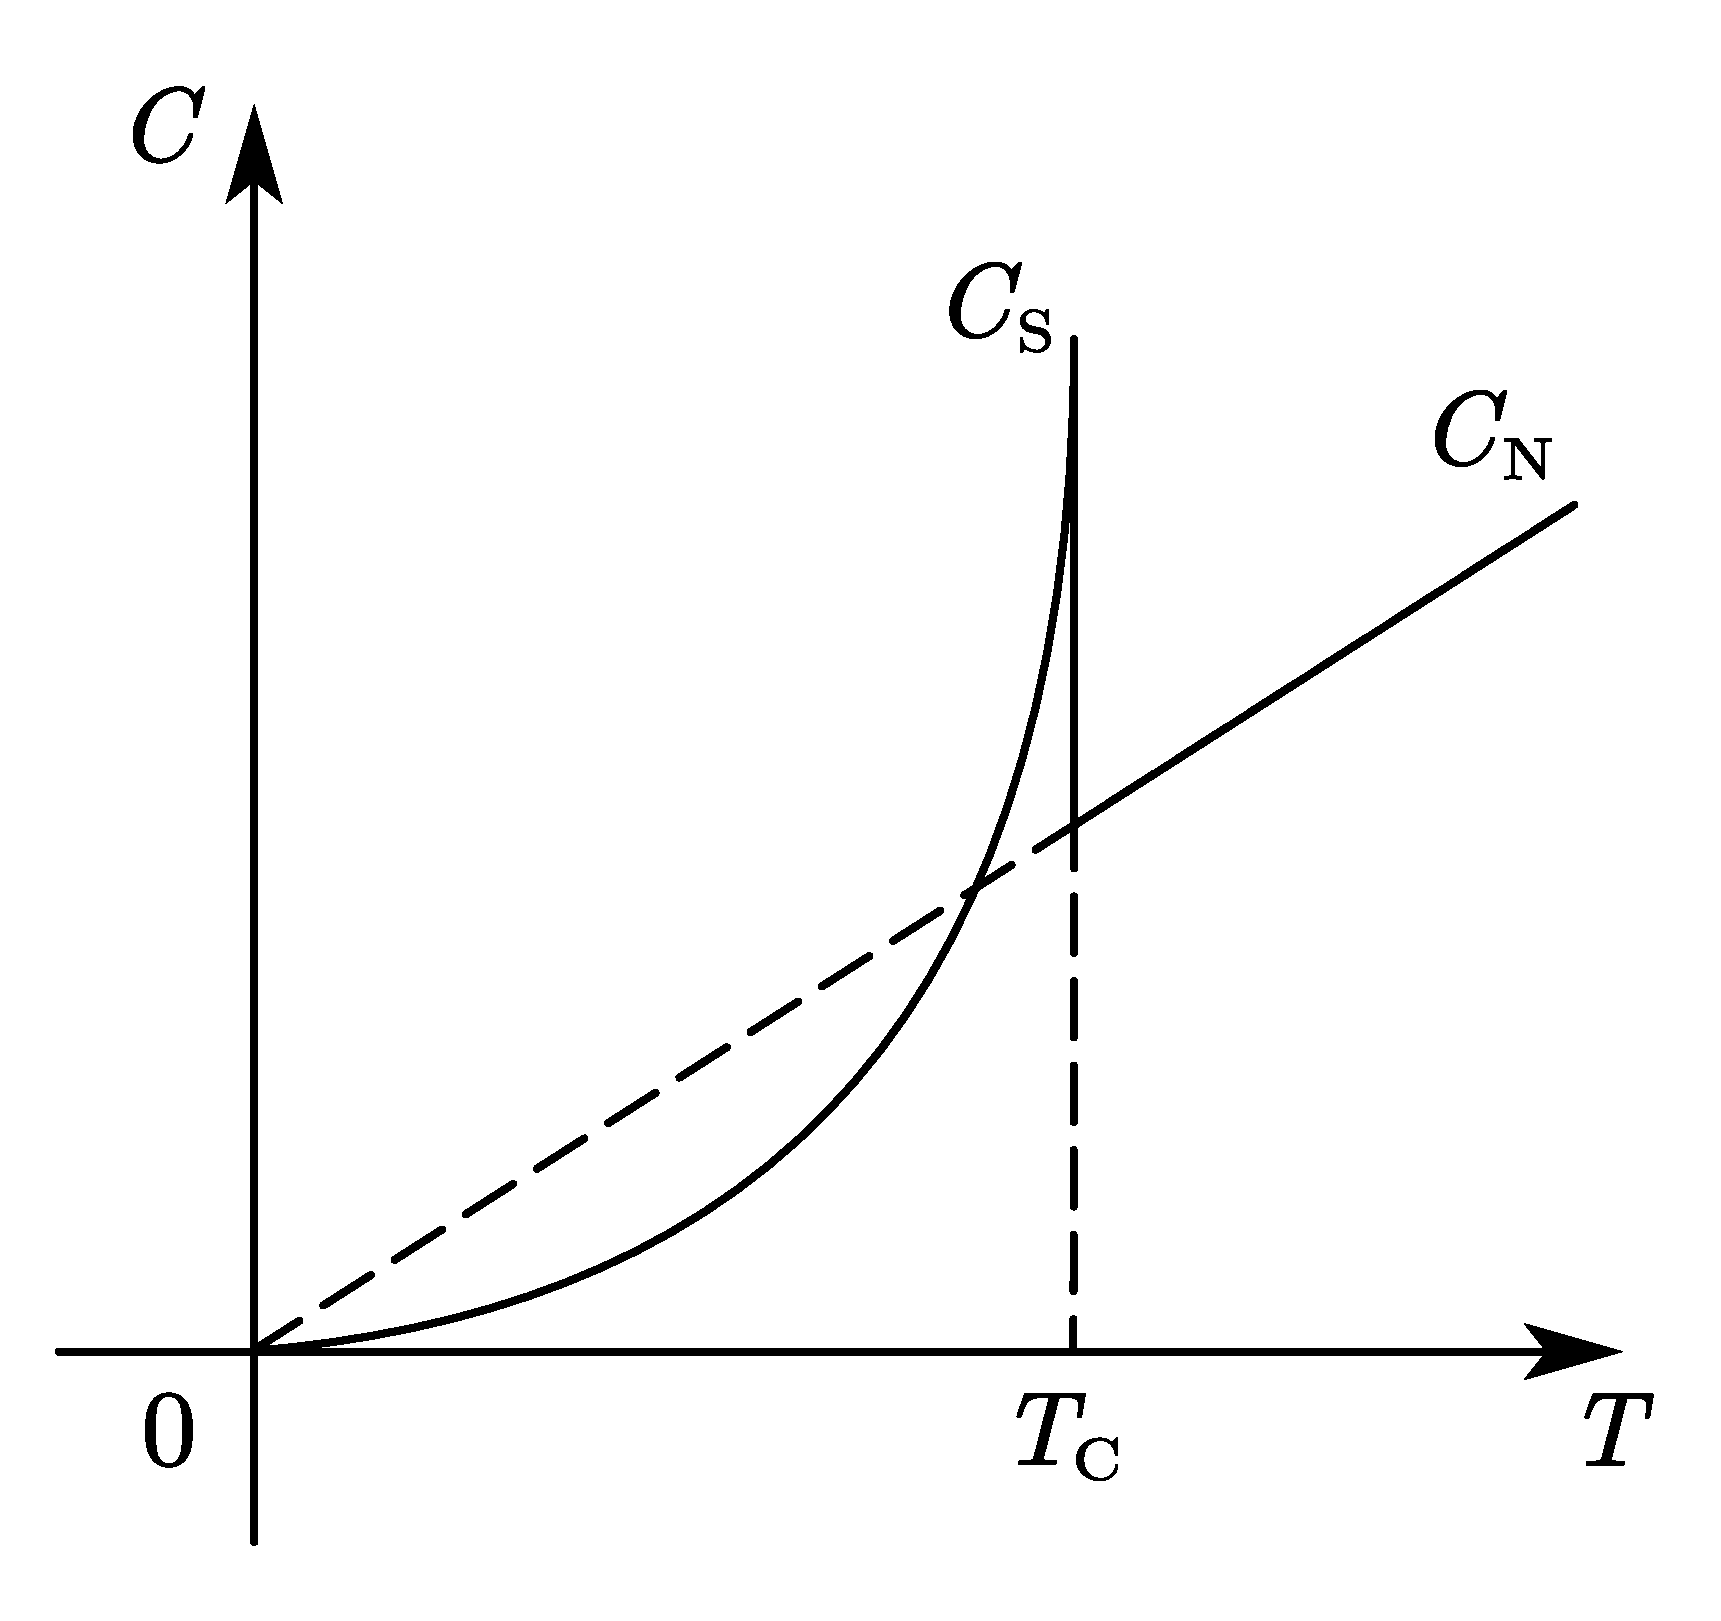
\includegraphics[width=6cm]{figure/sc1.pdf}
    \caption{超导电子比热.}
    \label{sc1}
\end{figure}

临界磁场具有表达式
\begin{equation}
    \left\{
        \begin{aligned}
            &H_{\fun{C}}(T)=H_{\fun{C}}(0)\lmi 1-1.06\ls \frac{T}{T_{\fun{C}}} \rs^2 \rmi,\quad (T\ll T_{\fun{C}}),\\
            &H_{\fun{C}}(T)=1.74 H_{\fun{C}}(0)\ls 1-\frac{T}{T_{\fun{C}}} \rs,\quad (T_{\fun{C}}-T\ll T_{\fun{C}}),
        \end{aligned}
    \right.
\end{equation}
这与 BCS 理论给出的结果一致, 如图 \ref{sc2} 所示.
\begin{figure}[htbp]
    \centering
    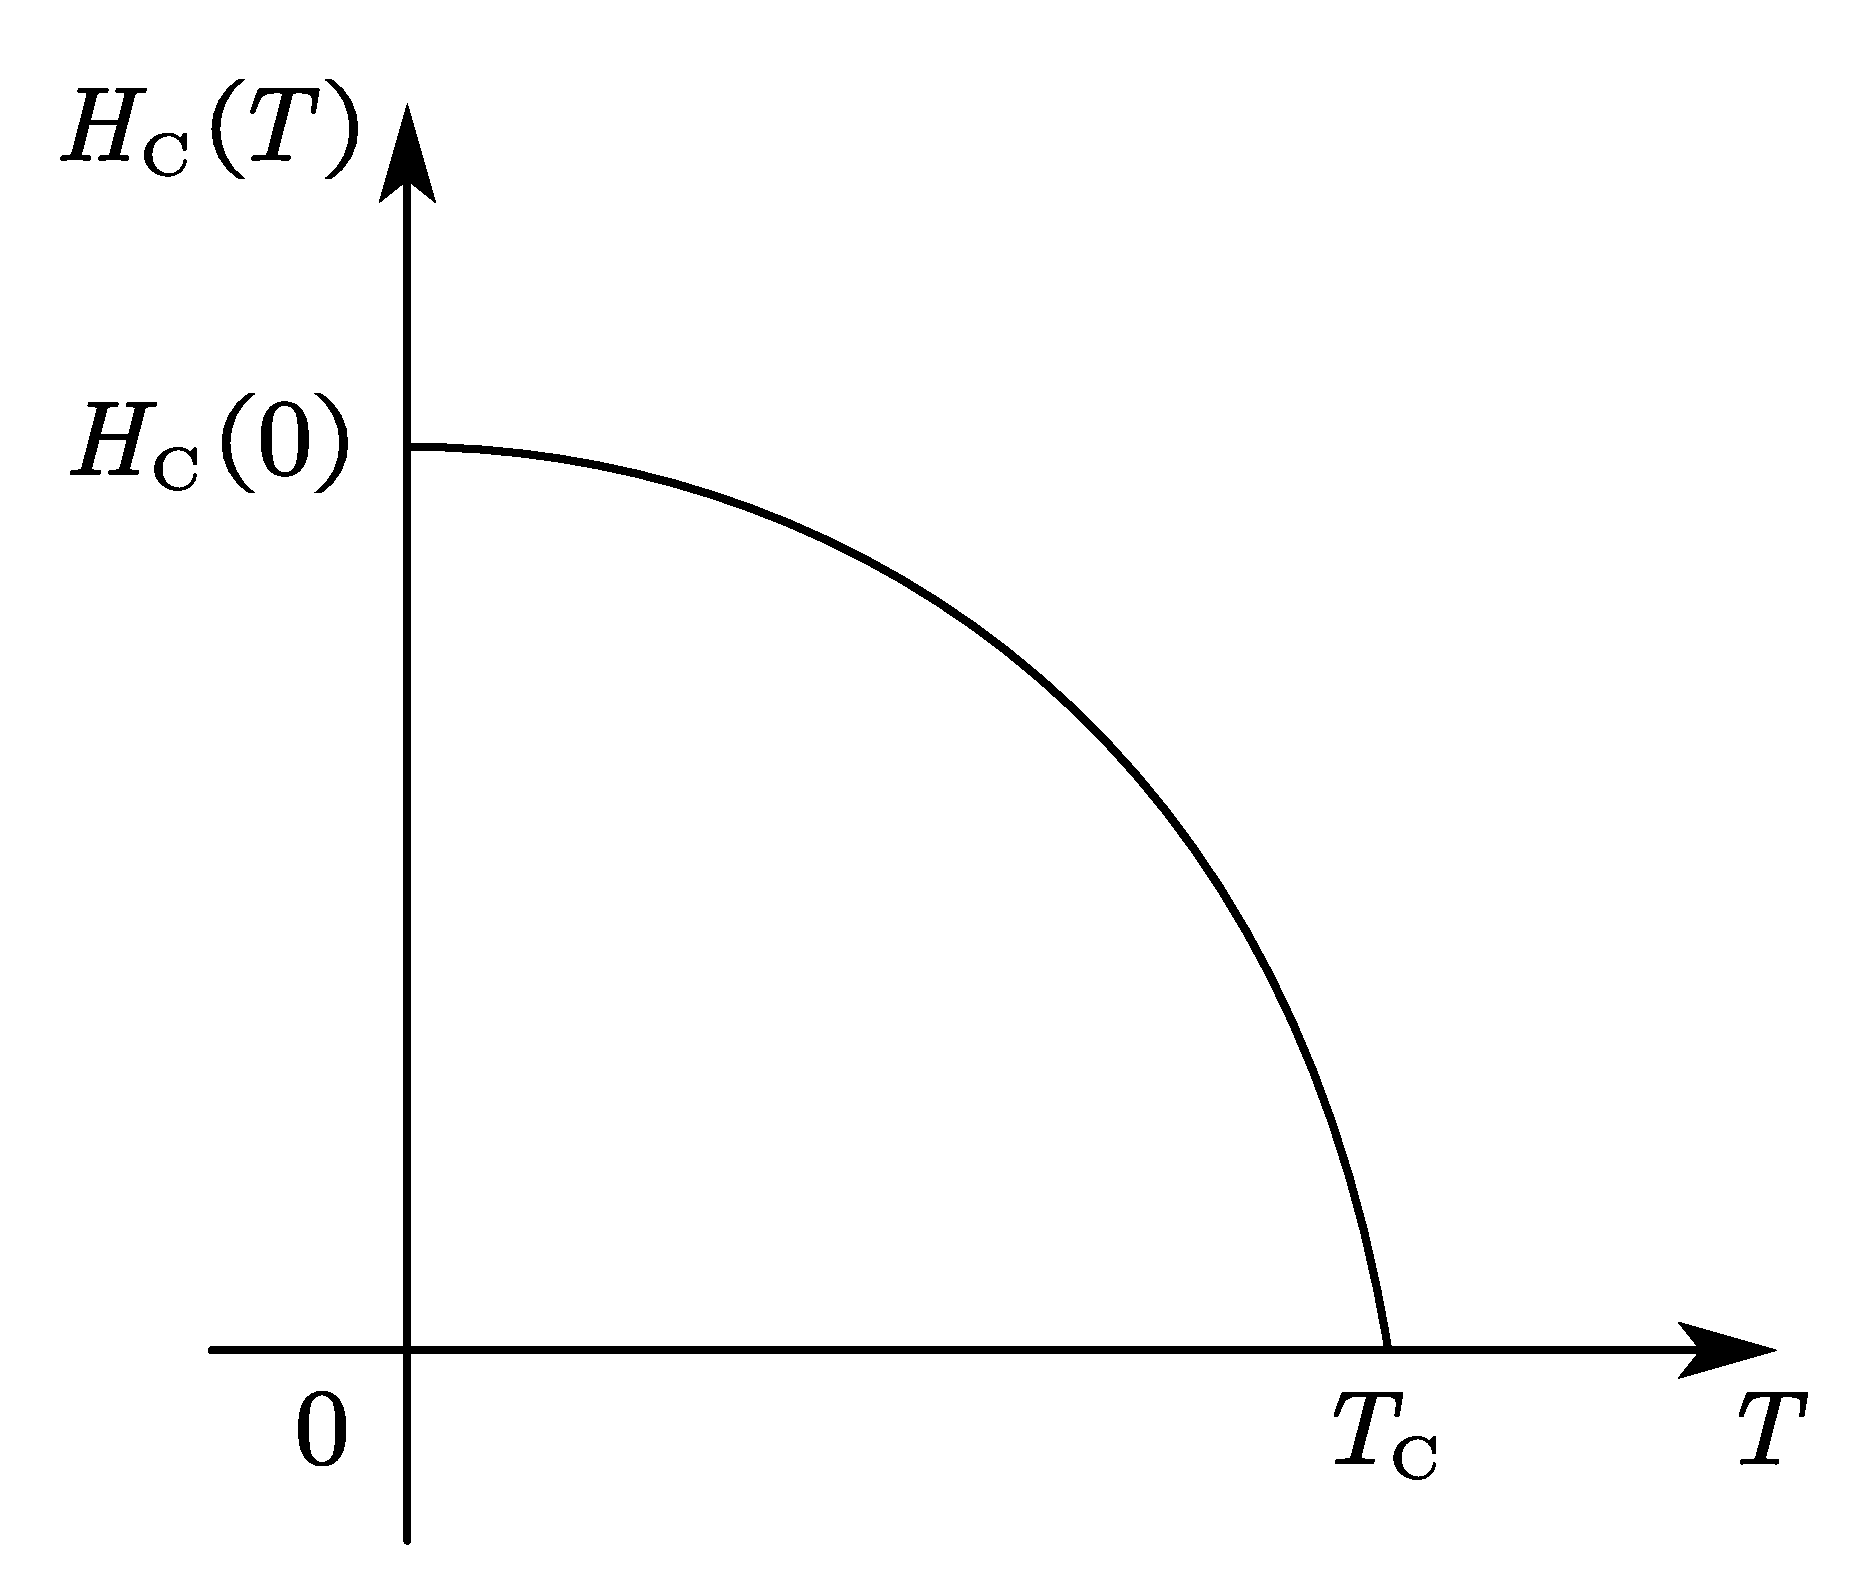
\includegraphics[width=6.5cm]{figure/sc2.pdf}
    \caption{超导电子临界磁场随温度变化.}
    \label{sc2}
\end{figure}

(c) 超导电子动量分布与态密度

计算超导电子的粒子数期望值:
 \begin{align}
        \lag\hat{N}\rag=&2V\frac{1}{\beta}\sum_{\omega_n}\int\frac{\dd\vct{k}}{(2\pi)^3}\mathcal{G}(\vct{k},\ii\omega_n)\e^{\ii\omega_n\eta}\nonumber\\
        =&2V\frac{1}{\beta}\sum_{\omega_n}\int\frac{\dd\vct{k}}{(2\pi)^3}\ls \frac{u_k^2}{\ii\omega-E_k}+\frac{v_k^2}{\ii\omega+E_k} \rs\e^{\ii\omega_n\eta}\nonumber\\
        =&2V\int\frac{\dd\vct{k}}{(2\pi)^3}\lmi u_k^2n_{\fun{F}}(E_k)+v_k^2n_{\fun{F}}(-E_k) \rmi\nonumber\\
        =&2\sum_k\lmi u_k^2n_{\fun{F}}(E_k)+v_k^2n_{\fun{F}}(-E_k) \rmi,
    \end{align}
其中费米分布的表达式为 
\begin{equation}
    n_{\fun{F}}(E_k)=\frac{1}{\e^{\beta E_k}+1},
\end{equation}
设粒子数分布与自旋指标无关, 则算符和期望值可以在形式上表示成 
\begin{equation}
    \hat{N}=\sum_{k\sigma}\hat{C}_{k\sigma}^\dg \hat{C}_{k\sigma}^{ },\quad \lag \hat{N} \rag=\sum_{k\sigma}\lag \hat{C}_{k\sigma}^\dg \hat{C}_{k\sigma}^{ } \rag=2\sum_k\lag \hat{C}_k^\dg \hat{C}_k^{ } \rag,
\end{equation}
令 
\begin{equation}
    \lag \hat{C}_k^\dg \hat{C}_k^{ } \rag\equiv n_k,
\end{equation}
就得到超导电子的动量分布为 
\begin{equation}
    n_k=u_k^2 n_{\fun{F}}(E_k)+v_k^2n_{\fun{F}}(-E_k).
\end{equation}
当 $T=0$ 时, 有 $n_k=v_k^2$. 在超导电子的动量分布中, 超导态的电子会增加动能, 但是 Cooper pair 的势能减少得更多. 这是一种与 Pauli 不相容原理相关的多体关联效应. 超导电子的动量分布如图 \ref{sc3} 所示.
\begin{figure}[htbp]
    \centering
    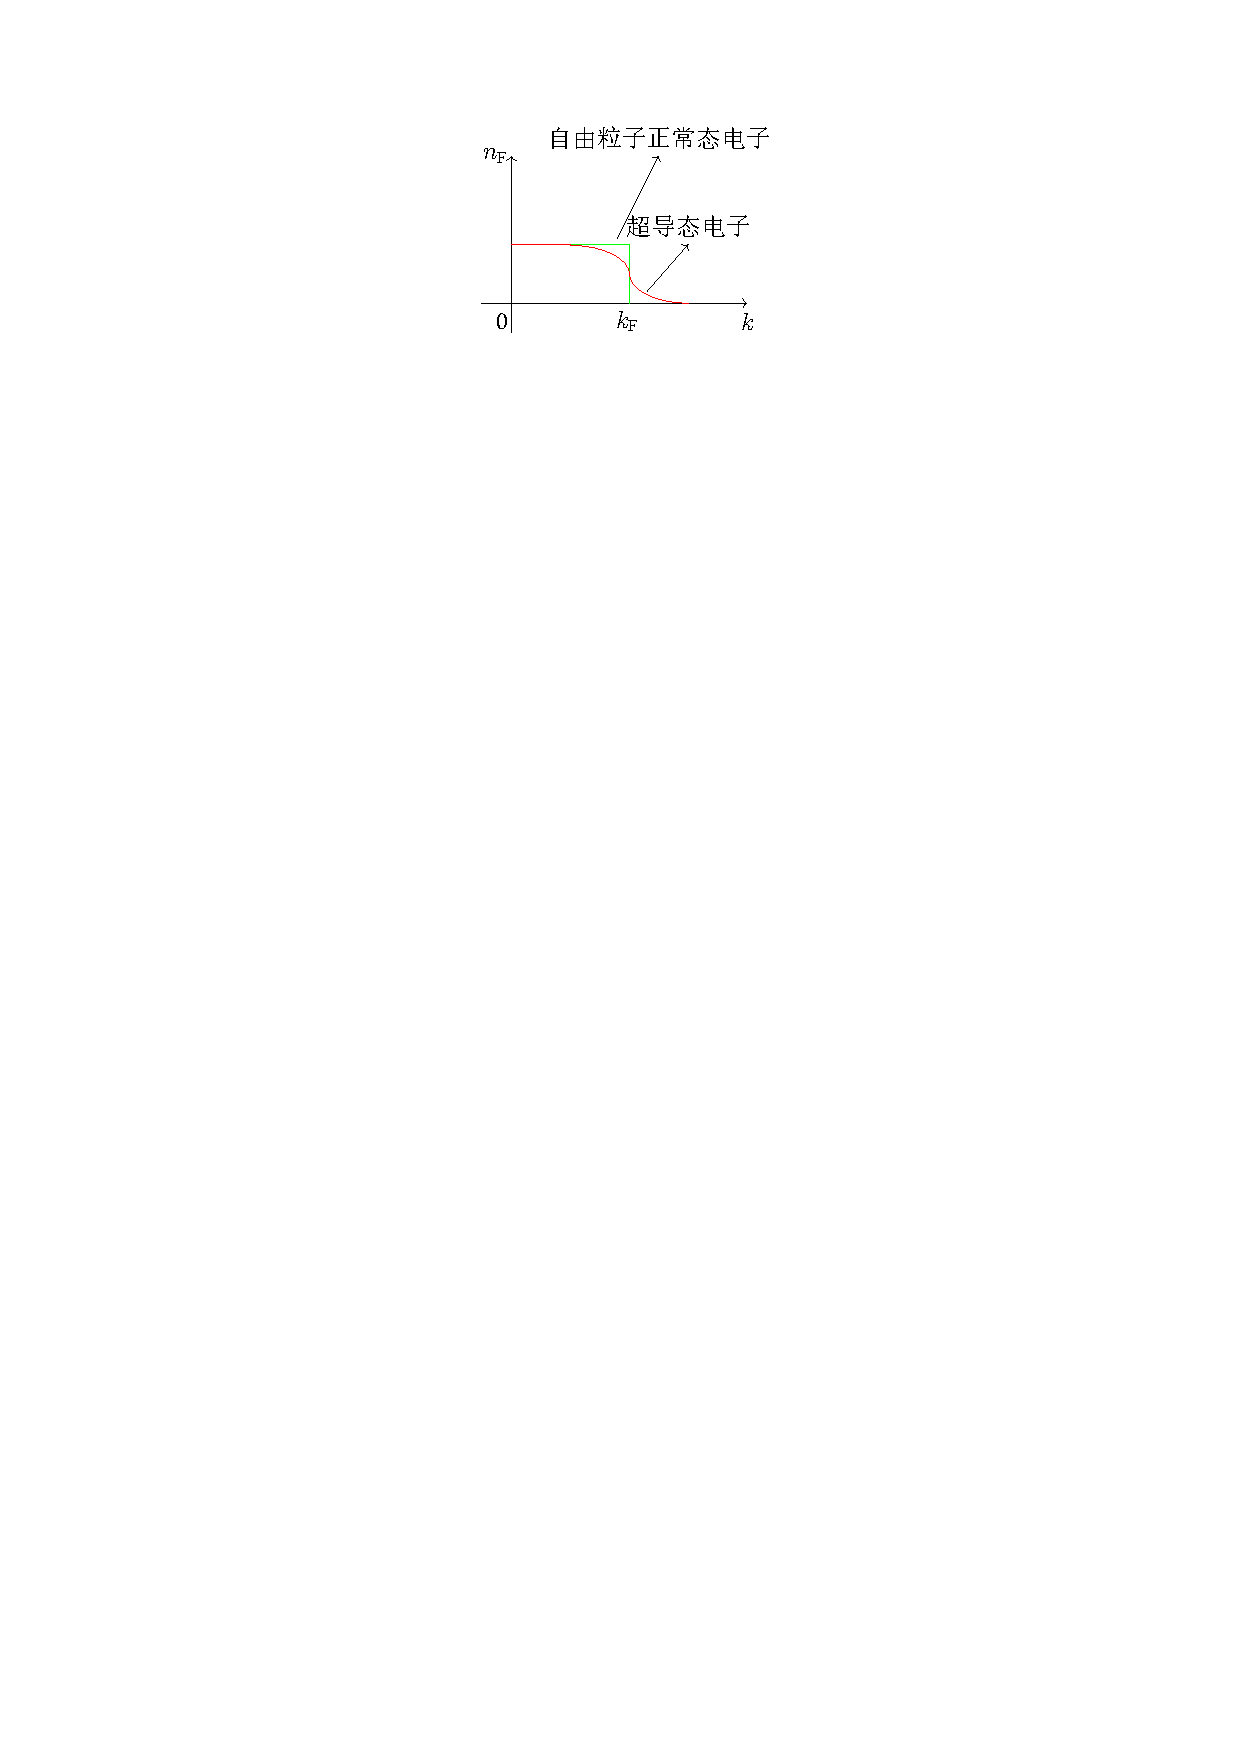
\includegraphics[width=6.5cm]{figure/sc3.pdf}
    \caption{超导电子的动量分布.}
    \label{sc3}
\end{figure}

重新将 $\lag N \rag$ 变形, 有 
 \begin{align}
        \lag N \rag=&2V\int\frac{\dd\vct{k}}{(2\pi)^3}\lmi u_k^2 n_{\fun{F}}(E_k)+v_{\fun{F}}^2n_{\fun{F}}(-E_k) \rmi\nonumber\\
        =&2\int\dd\omega n_{\fun{F}}(\omega)\sum_k\lmi u_k^2\delta(\omega-E_k)+v_k^2\delta(\omega+E_k) \rmi\nonumber\\
        \equiv &2\int\dd\omega n_{\fun{F}}(\omega)N_{\fun{S}}(\omega),
    \end{align}
其中 $N_{\fun{S}}(\omega)$ 的物理意义是 $\omega$ 态粒子的态密度, 表达式可以写成 
  \begin{align}
        N_{\fun{S}}(\omega)=&\sum_k\lmi u_k^2\delta(\omega-E_k)+v_{k}^2\delta(\omega+E_k) \rmi\nonumber\\
        =&\sum_k A(\vct{k},\omega),
    \end{align}
其中谱函数 $A(\vct{k},\omega)$ 与推迟格林函数有直接联系: 
\begin{equation}
    A(\vct{k},\omega)=-\frac{1}{\pi}\fun{Im}G^{R}(\vct{k},\ii\omega),
\end{equation}
所以电子态密度可以表示成 
\begin{equation}
    N_{\fun{S}}(\vct{k})=\sum_k -\frac{1}{\pi} \fun{Im}G^R(\vct{k},\ii\omega),
\end{equation}
根据松原格林函数和热力学推迟格林函数之间的关系, 可以直接得到推迟格林函数的表达式 
 \begin{align}
        \mathcal{G}(\vct{k},\ii\omega_n\to \omega+\ii\eta)=&G^R(\vct{k},\omega)\nonumber\\
        =&\frac{u_k^2}{\omega-E_k+\ii\eta}+\frac{v_k^2}{\omega+E_k+\ii\eta}.
    \end{align}
超导电子态密度分布如图 \ref{sc4} 所示, 这一结果与实验测得结果一致.

\begin{figure}[htbp]
    \centering
    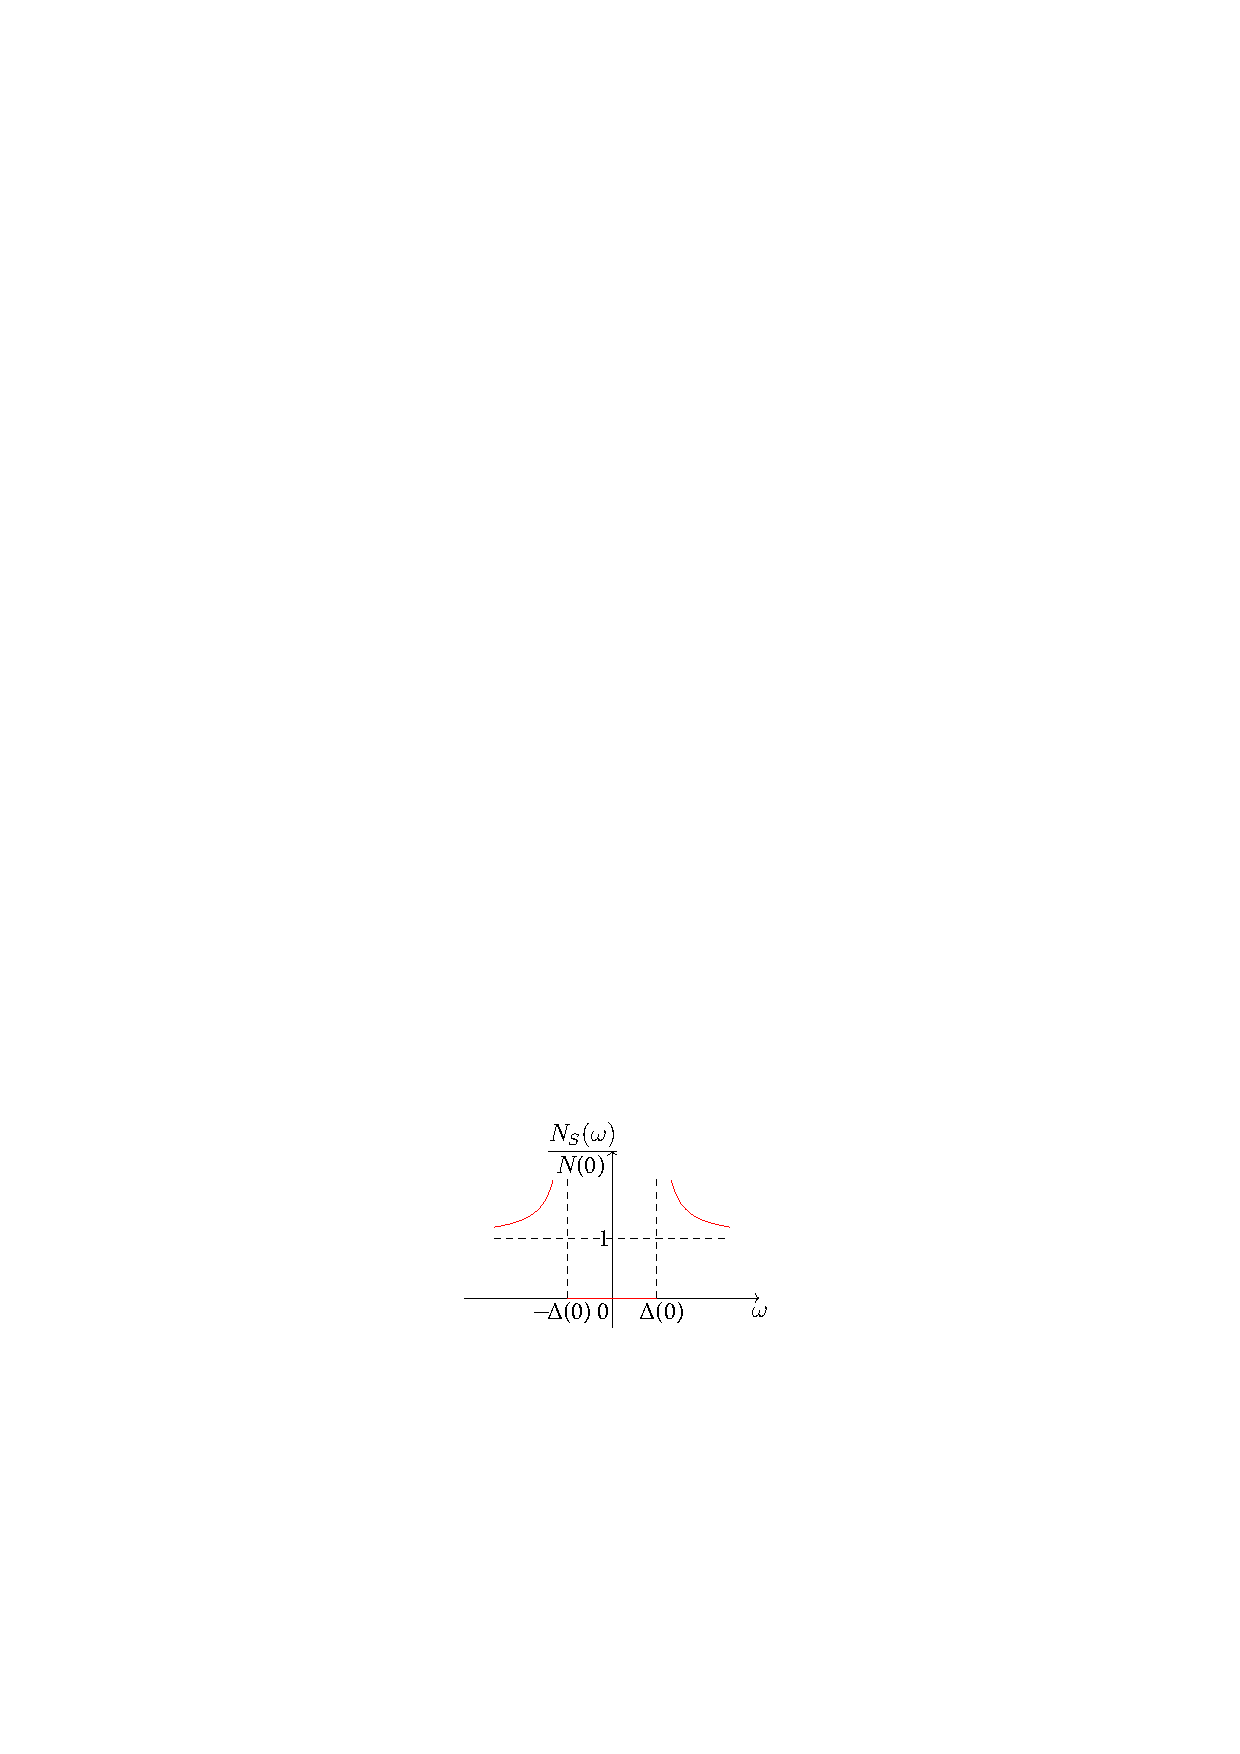
\includegraphics[width=7cm]{figure/sc4.pdf}
    \caption{超导电子态密度分布.}
    \label{sc4}
\end{figure}

另外, 根据谱定理, 有 
   \begin{align}
        \llag \hat{C}_k^\dg \hat{C}_k^{ } \rrag=&2\sum_k\int_{-\infty}^{\infty}\frac{-\frac{1}{\pi}\fun{Im}G^{R}(\vct{k},\omega)}{\e^{\beta\omega}+1}\dd\omega\nonumber\\
        \equiv &2\int\dd\omega n_{\fun{F}}(\omega)N_{\fun{S}}(\omega),
    \end{align}
从而有 
\begin{equation}
    N_{\fun{S}}(\omega)=\sum_k-\frac{1}{\pi}\fun{Im}G^R(\vct{k},\omega),
\end{equation}
这与前面得到的结果一致. 

\setcounter{chapter}{4}
\chapter{相干态路径积分及其应用}
\begin{introduction}
\item 谐振子相干态
\item 多体理论中的玻色子系统相干态
\item 多体理论中的费米子系统相干态
\item Stratonovich-Hubbard 变换
\item 路径积分方法在超导理论中的应用
\end{introduction}
\section{谐振子相干态}
一维谐振子的哈密顿量可以写为如下形式:
\begin{equation}
\hat{H}=\left(\hat{a}^{\dagger} \hat{a}+\frac{1}{2}\right) \hbar\omega,
\end{equation}
这里$\hat{a}^\dagger$、$\hat a$分别是产生、消灭算符, 满足如下玻色子对易关系:
\begin{equation}
\left[\hat{a}, \hat{a}^{\dagger}\right]_{-}=1,\quad\left[\hat{a}, \hat{a}\right]_{-}=\left[\hat{a}^{\dagger}, \hat{a}^{\dagger}\right]_{-}=0.
\end{equation}

产生、消灭算符本身不是厄米算符, 但两者的乘积可以构成厄米算符:
\begin{equation}
\hat{N}=\hat{a}^{\dagger} \hat{a},
\end{equation}
即粒子数算符. 粒子数算符与哈密顿量对易, 可以得到共同本征态 $|n\rangle(n=0,1,2, \cdots)$ 满足如下本征方程:
\begin{align}
&\hat{N}|n\rangle=n|n\rangle, \nonumber\\
&\hat{H}|n\rangle=\left(n+\frac{1}{2}\right)\hbar \omega|n\rangle .
\end{align}
同样可以证明 $|n\rangle$ 是一组正交完备的本征态, 满足如下关系:
\begin{align}
\sum_{n}|n\rangle\langle n| &=\mathbbm 1 &\text {(完备性), }\nonumber\\
\left.\left\langle n^{\prime}\right| n\right\rangle &=\delta_{n n^{\prime}} & \text{(正交性). }
\end{align}
定义粒子真空态 $|0\rangle$, 满足:
\begin{equation}
\hat{a}|0\rangle=0,
\end{equation}
一般地, 有:
\begin{align}
|n\rangle&=\frac{\left(\hat{a}^{\dagger}\right)^n}{\sqrt{n!}}|0\rangle,\nonumber\\
\hat{a}^{\dagger}|n\rangle &=\sqrt{n+1}|n+1\rangle, \nonumber\\
\hat{a}|n\rangle &=\sqrt{n}|n-1\rangle .
\end{align}


下面在谐振子本征态的基础上引入谐振子相干态, 即消灭算符的本征态:
\begin{equation}
\hat{a}|\alpha\rangle=\alpha|\alpha\rangle,
\end{equation}
其共轭式为:
\begin{equation}
\langle\alpha| \hat{a}^{\dagger}=\alpha^{*}\langle\alpha| .
\end{equation}
这里 $\alpha$ 是一个复数, 且 $|\alpha\rangle$ 具有如下形式:
\begin{equation}
|\alpha\rangle=\e^{-\frac{|\alpha|^{2}}{2}} \e^{\alpha \hat{a}^{\dagger}}|0\rangle,
\end{equation}
前面的常数因子是归一化常数. 

相干态首先是归一的, 即
\begin{equation}
\left.\left\langle\alpha \right| \alpha\right\rangle=1.
\end{equation}
但其一般不正交，有如下关系:
\begin{equation}
\left.\left\langle\alpha^{\prime} \right| \alpha\right\rangle=\exp \left[-\frac{|\alpha|^2}{2}-\frac{\left|\alpha^{\prime}\right|^{2}}{2}+\alpha \alpha^{\prime *}\right],
\end{equation}
进一步可以得到:
\begin{equation}
\left.\left|\left\langle\alpha^{\prime} \right| \alpha\right\rangle\right|^{2}=\e^{-\left|\alpha-\alpha^{\prime}\right|^{2}},
\end{equation}
在复平面上, 当 $\left|\alpha-\alpha^{\prime}\right| \rightarrow \infty$ 时, 有 $\left\langle\alpha^{\prime} \mid \alpha\right\rangle \rightarrow 0$, 这时两个态近似正交.谐振子的相干态虽然不正交, 却是一组完备基, 这种性质称为\textbf{超完备性}. 有如下完备性关系:
\begin{equation}
\int \frac{\mathrm{d}^{2} \alpha}{\pi}|\alpha\rangle\langle\alpha|=\mathbbm{1},
\end{equation}
其中积分测度为:
\begin{equation}
\mathrm{d}^{2} \alpha=\mathrm{d} (\operatorname{Re}\alpha) \mathrm{d} (\operatorname{Im}\alpha).
\end{equation}
取$\alpha = x+\mathrm i y,\alpha^*=x-\mathrm i y$，则
\begin{equation}
\mathrm{d} (\operatorname{Re}\alpha)=\mathrm{d} x, \quad \mathrm{d} (\operatorname{Im}\alpha)=\mathrm{d} y ,
\end{equation}
这样完备性条件可以写为:
\begin{equation}
\iint \frac{\mathrm{d} x \mathrm{d} y}{\pi}|\alpha\rangle\langle\alpha|=\mathbbm 1 .
\end{equation}

由于相干态具有完备性, 可以利用相干态展开任意态, 称这种表象为\textbf{相干态表象}:
\begin{equation}
|\psi\rangle=\int \frac{\mathrm{d}^{2} \alpha}{\pi}|\alpha\rangle\langle\alpha | \psi\rangle,
\end{equation}
但是由于超完备性, 这种展开并不唯一. 同样, 算符也可以展开为:
\begin{equation}
\hat{A}=\int \frac{\mathrm{d}^{2} \alpha}{\pi} \int \frac{\mathrm{d}^{2} \alpha^{\prime}}{\pi}|\alpha\rangle\langle\alpha|\hat{A}| \alpha^{\prime}\rangle\langle\alpha^{\prime}| .
\end{equation}
可以得到如下关系:
\begin{align}
\hat{a}|\alpha\rangle &=\alpha|\alpha\rangle, \nonumber\\
\langle\alpha| \hat{a}^{\dagger} &=\langle\alpha| \alpha^{*}, \nonumber\\
\hat{a}^{\dagger}|\alpha\rangle &=\left(\frac{\partial}{\partial \alpha}+\frac{\alpha^{*}}{2}\right)|\alpha\rangle, \nonumber\\
\langle\alpha| \hat{a} &=\left(\frac{\partial}{\partial \alpha^{*}}+\frac{\alpha}{2}\right)\langle\alpha| .
\end{align}
特别地, 对体系本征态求迹可以写为对相干态的“求迹”:
\begin{align}
\operatorname{Tr} \hat{A} &=\sum_{n}\langle n|\hat{A}| n\rangle\nonumber\\
&=\sum_{n}\left\langle n\left|\int \frac{\mathrm{d}^{2} \alpha}{\pi}\right| \alpha\right\rangle\langle\alpha|\hat{A}| n\rangle \nonumber\\
&=\int \frac{\mathrm{d}^{2} \alpha}{\pi} \sum_{n}\langle n | \alpha\rangle\langle\alpha|\hat{A}| n\rangle\nonumber\\
&=\int \frac{\mathrm{d}^{2} \alpha}{\pi} \sum_{n}\langle\alpha|\hat{A}| n\rangle\langle n |\alpha\rangle \nonumber\\
&=\int \frac{\mathrm{d}^{2} \alpha}{\pi}\langle\alpha|\hat{A}| \alpha\rangle.
\end{align}


\section{多体理论中的玻色子系统相干态}
前面已经介绍了一维谐振子相干态, 而对于全同粒子体系, 每一个单粒子态都对应着不同的相干态. 下面介绍凝聚态场论中全同玻色子系统的相干态. 为简单起见, 先从单分量的情况考虑, 这实际上就是一维谐振子相干态.

\subsection{单分量玻色子相干态}
场论中我们用 $|\phi\rangle$ 代替 $|\alpha\rangle$ 表示相干态, 这里 $|\phi\rangle$ 仍然是消灭算符的本征态. 为方便起见, 凝聚态场论中考虑如下没有归一化的相干态:
\begin{equation}
|\phi\rangle\equiv\e^{\phi \hat{a}^{\dagger}}|0\rangle,
\end{equation}
这里 $\phi$ 仍是复数, $|0\rangle$ 是粒子真空态. 有如下本征方程:
\begin{equation}
\hat{a}|\phi\rangle=\phi|\phi\rangle,
\end{equation}
上式的厄米共轭为:
\begin{equation}
\langle\phi| \hat{a}^{\dagger}=\phi^{*}\langle\phi|,
\end{equation}
可以得到如下关系:
\begin{equation}
\left\{\begin{aligned}
\hat{a}^{\dagger}|\phi\rangle &=\frac{\partial}{\partial \phi}|\phi\rangle, \\
\langle\phi| \hat{a} &=\frac{\partial}{\partial \phi^{*}}\langle\phi| .
\end{aligned}\right.
\end{equation}

下面讨论单分量情况玻色子系统相干态的性质:
\begin{itemize}
\item 内积(非正交归一) \\
凝聚态场论中用到的相干态是非归一化的, 而且相干态本身不同的态之间不正交，一般有如下关系:
\begin{equation}
\langle\phi| \phi\rangle=\e^{\phi^{*} \phi}=\e^{|\phi|^{2}}.
\end{equation}
\begin{proof}
\begin{align}
\langle\phi | \phi\rangle &=\left\langle 0\left|\e^{\hat{a} \phi^{*}} \e^{\phi \hat{a}^{\dagger}}\right| 0\right\rangle\\
&=\left\langle 0\left|\sum_{m} \frac{\left(\hat{a} \phi^{*}\right)}{m !} \sum_{n} \frac{\phi \hat{a}^{\dagger}}{n !}\right| 0\right\rangle \nonumber\\
&=\sum_{m} \sum_{n} \frac{\left(\phi^{*}\right)^{m}}{m !} \frac{\phi^{n}}{n !}\left\langle 0\left|\hat{a}^{m}\left(\hat{a}^{\dagger}\right)^{n}\right| 0\right\rangle\nonumber\\
&=\sum_{m} \sum_{n} \frac{\left(\phi^{*}\right)^{m}}{m !} \frac{\phi^{n}}{n !}\langle m|\sqrt{m !} \sqrt{n !}| n\rangle \nonumber\\
&=\sum_{m} \sum_{n} \frac{(\phi^{*})^{m}}{m !} \frac{\phi^{n}}{n !} \sqrt{m !} \sqrt{n !} \delta_{m n}\nonumber\\
&=\sum_{n} \frac{\left(\phi^{*} \phi\right)^{n}}{n !} \nonumber\\
&=\e^{\phi^{*} \phi}.
\end{align}
\end{proof}
一般地, 有:
\begin{equation}
\langle\phi^\prime | \phi\rangle=\e^{\phi^{\prime *} \phi}.
\end{equation}

\item 完备性\\
相干态本身具有超完备性, 但是这里我们使用的是未归一化的相干态, 所以单位算符和前面的形式有所不同:
\begin{equation}
\int \frac{\mathrm{d}^{2} \phi}{\pi} \e^{-\phi^{*} \phi}|\phi\rangle\langle\phi|=\mathbbm 1 .
\end{equation}
\end{itemize}

同样地, 可以在相干态表象下对算符求迹:
\begin{equation}
\operatorname{Tr} \hat{A}=\int \frac{\mathrm{d}^{2} \phi}{\pi} \e^{-\phi^{*} \phi}\langle\phi|\hat{A}| \phi\rangle,
\end{equation}
这是下面推导配分函数路径积分形式的基础.

考虑 $\hat{H}$ 写成了产生、消灭算符的函数形式 $\hat{H}\left(\hat{a}^{\dagger}, \hat{a}\right)$, 而且产生、消灭算符是按正规乘积的顺序排列的, 则单分量玻色子情况的配分函数函数可以写成如下求迹的形式:
\begin{equation}
\mathcal{Z}=\operatorname{Tr}\left[\e^{-\beta \hat{H}\left(\hat{a}^{\dagger}, \hat{a}\right)}\right]=\int \frac{\mathrm{d}^{2} \phi}{\pi} \e^{-\phi^{*} \phi}\left\langle\phi\left|\e^{-\beta \hat{H}\left(\hat{a}^{\dagger}, \hat{a}\right)}\right| \phi\right\rangle.
\end{equation}
按量子力学中路径积分的方法, 把 $\beta$ 看成是时间(虚时), 分为 $N$ 个等份, 每一份为 $\displaystyle \Delta \tau=\frac{\beta}{N}$, 得到:
\begin{align}
\left\langle\phi\left|\e^{-\beta \hat{H}}\right| \phi\right\rangle &=\left\langle\phi\left|\left(\e^{-\Delta \tau \hat{H}}\right)^{N}\right| \phi\right\rangle \nonumber\\
&=\left\langle\phi\left|\e^{-\Delta \tau \hat{H}} \cdots \e^{-\Delta \tau \hat{H}} \cdots \e^{-\Delta \tau \hat{H}}\right| \phi\right\rangle,
\end{align}
在任意两个相邻 $\e^{-\Delta \tau \hat{H}}$ 之间插入单位算符 $\displaystyle\int \frac{\mathrm{d}^{2} \phi}{\pi} \e^{-\phi^{*} \phi}|\phi\rangle\langle\phi|$, 得到:
\begin{align}
\left\langle\phi\left|\e^{-\beta \hat{H}}\right| \phi\right\rangle=& \int \frac{\mathrm{d}^{2} \phi_{1}}{\pi} \cdots \frac{\mathrm{d}^{2} \phi_{N-1}}{\pi} \e^{-\phi_{1}^{*} \phi^{}_{1}} \cdots \e^{-\phi_{j}^{*} \phi^{}_{j}} \cdots \e^{\phi_{N-1}^{*} \phi^{}_{N-1}} \nonumber\\
&\times\left\langle\phi\left|\e^{-\Delta \tau \hat{H}}\right| \phi_{N-1}\right\rangle \cdots\left\langle\phi_{j}\left|\e^{-\Delta \tau \hat{H}}\right| \phi_{j-1}\right\rangle \cdots\left\langle\phi_{1}\left|\e^{-\Delta \tau \hat{H}}\right| \phi\right\rangle,
\end{align}
为了方便表示, 令:
\begin{equation}
|\phi\rangle \equiv\left|\phi_{0}\right\rangle, \quad\langle\phi| \equiv\left\langle\phi_{N}\right|,
\end{equation}
实际上 $\phi_{0}=\phi_{N}$. 考虑 $N \rightarrow \infty, \Delta\tau \rightarrow 0^{+}$ 是小量, 展开到一阶, 这时上式中的通项可以展开为:
\begin{align}
\left\langle\phi_{j}\left|\e^{-\Delta \tau \hat{H}}\right| \phi_{j-1}\right\rangle & \approx\left\langle\phi_{j}\left|(1-\Delta \tau \hat{H})\right| \phi_{j-1}\right\rangle \nonumber\\
&=\left.\left\langle\phi^{}_{j} \right| \phi^{}_{j-1}\right\rangle-\Delta \tau\left\langle\phi^{}_{j}\left|\hat{H}\left(\hat{a}^{\dagger}, \hat{a}\right)\right| \phi^{}_{j-1}\right\rangle \nonumber\\
&=\left.\left\langle\phi^{}_{j} \right| \phi^{}_{j-1}\right\rangle-\Delta \tau\left\langle\phi^{}_{j}\left|H\left(\phi_{j}^{*}, \phi^{}_{j-1}\right)\right| \phi^{}_{j-1}\right\rangle\nonumber \\
&=\left[1-\Delta \tau H\left(\phi_{j}^{*}, \phi^{}_{j-1}\right)\right]\left.\left\langle\phi^{}_{j} \right| \phi^{}_{j-1}\right\rangle \nonumber\\
&=\e^{-\Delta \tau H\left(\phi_{j}^{*}, \phi^{}_{j-1}\right)} \e^{\phi_{j}^{*} \phi^{}_{j-1}}.
\end{align}
定义
\begin{equation}
\mathscr{D}_{N}\left(\phi^{*}, \phi\right)=\prod_{j=1}^{N}\left(\frac{\mathrm{d}^{2} \phi_{j}}{\pi}\right),
\end{equation}
这样配分函数可以写为:
\begin{align}
\mathcal{Z} &=\lim _{N \rightarrow \infty} \int \mathscr{D}_{N}\left(\phi^{*}, \phi\right) \exp \left\{-\sum_{j=1}^{N}\left[\phi_{j}^{*}\left(\phi^{}_{j}-\phi^{}_{j-1}\right)+\Delta \tau H\left(\phi_{j}^{*}, \phi^{}_{j-1}\right)\right]\right\} \nonumber\\
&=\lim _{N \rightarrow \infty}\int \mathscr{D}_{N}\left(\phi^{*}, \phi\right) \exp \left\{-\Delta \tau \sum_{j=1}^{N}\left[ \frac{\phi_{j}^{*}\left(\phi^{}_{j}-\phi^{}_{j-1}\right)}{\Delta \tau}+H\left(\phi_{j}^{*}, \phi^{}_{j-1}\right)\right]\right\} \nonumber\\
&\equiv\lim _{N \rightarrow \infty} \int \mathscr{D}_{N}\left(\phi^{*}, \phi\right) \e^{-S_{N}},
\end{align}
其中
\begin{equation}
S_{N}=\Delta \tau \sum_{j=1}^{N}\left[ \frac{\phi_{j}^{*}\left(\phi^{}_{j}-\phi^{}_{j-1}\right)}{\Delta \tau}+H\left(\phi_{j}^{*}, \phi^{}_{j-1}\right)\right]
\end{equation}
是作用量. 当 $N \to\infty$ 时, 进一步做变换:
\begin{align}
\phi_{j} & \rightarrow \phi(\tau), \nonumber\\
\frac{\phi_{j}^{*}\left(\phi^{}_{j}-\phi^{}_{j-1}\right)}{\Delta \tau}& \rightarrow \phi^{*}(\tau) \frac{\partial}{\partial \tau} \phi(\tau), \nonumber\\
\sum_{j=1}^{N}\Delta \tau & \rightarrow \int_{0}^{\beta} \mathrm{d} \tau,\nonumber \\
\mathscr{D}_{N}\left(\phi^{*}, \phi\right) & \rightarrow \mathscr{D}\left(\phi^{*}, \phi\right),\nonumber\\
S_N&\rightarrow S,
\end{align}
可将离散情况连续化, 这里 $0<\tau<\beta$. 这样配分函数可以写为:
\begin{equation}
\mathcal{Z}=\int \mathscr{D}\left(\phi^{*}, \phi\right) \e^{-S\left(\phi^{*}, \phi\right)},
\end{equation}
其中作用量 $S$ 是 $\left(\phi^{*}, \phi\right)$ 的泛函:
\begin{equation}
S=\int_{0}^{\beta} \mathrm{d} \tau\left[\phi^{*}(\tau) \frac{\partial}{\partial \tau} \phi(\tau)+H\left(\phi^{*}(\tau), {\phi}(\tau)\right)\right],
\end{equation}
边界条件为:
\begin{equation}
\phi(0)=\phi(\beta), \quad \phi^{*}(0)=\phi^{*}(\beta).
\end{equation}

\begin{example}谐振子哈密顿量为:
\begin{equation}
\hat{H}=(\varepsilon-\mu) \hat{a}^{\dagger} \hat{a},
\end{equation}
此时的作用量为:
\begin{align}
S=&\int_{0}^{\beta} \mathrm{d} \tau\left[\phi^{*}(\tau) \frac{\partial}{\partial \tau} \phi(\tau)+H\left(\phi^{*}, {\phi}\right)\right]\nonumber\\
=&\int_{0}^{\beta} \mathrm{d} \tau \phi^{*}(\tau)\left[\frac{\partial}{\partial \tau}+(\varepsilon-\mu)\right] \phi(\tau) .
\end{align}
\end{example}

\subsection{多分量玻色子相干态}
多分量(多粒子)系统的相干态是单变量(单粒子)系统相干态的直积, 哈密顿量为
\begin{equation}
\hat H=\sum_k(\varepsilon_k^0-\mu) \hat{a}_k^{\dagger} \hat{a}^{}_k + \frac{1}{2}\sum_{kk^\prime}\sum_{q}V(\vct q)\hat{a}^{\dagger}_{k+q}\hat{a}^{\dagger}_{k^\prime-q}\hat{a}^{}_{k^\prime}\hat{a}^{}_{k},
\end{equation}
其中
\begin{equation}
\left[\hat{a}^{}_{k}, \hat{a}^{\dagger}_{k^\prime}\right]_{-}=\delta_{kk^\prime},\quad\left[\hat{a}^{}_{k}, \hat{a}^{}_{k^\prime}\right]_{-}=\left[\hat{a}_{k}^{\dagger}, \hat{a}_{k^\prime}^{\dagger}\right]_{-}=0.
\end{equation}
定义多分量系统相干态为:
\begin{equation}
|\phi\rangle \equiv \prod_{k} \e^{\phi^{}_{k} \hat{a}_{k}^{\dagger}}|0\rangle,
\end{equation}
这一相干态是任意单粒子态消灭算符 $\hat{a}_{k}$ 的本征态, 有如下本征方程:
\begin{equation}
\hat{a}_{k}|\phi\rangle=\phi_{k}|\phi\rangle,
\end{equation}
其厄米共轭为:
\begin{equation}
\langle\phi| \hat{a}^{\dagger}=\phi_{k}^{*}\langle\phi|.
\end{equation}
同样可以得到如下关系:
\begin{equation}
\left\{\begin{aligned}
\hat{a}_{k}^{\dagger}|\phi\rangle=\frac{\partial}{\partial \phi_{k}}|\phi\rangle, \\
\langle\phi| \hat{a}_{k}=\frac{\partial}{\partial \phi_{k}^{*}}\langle\phi| .
\end{aligned}\right.
\end{equation}

下面讨论多分量情况玻色子系统相干态的性质.
\begin{itemize}
\item 内积(非正交归一)
\begin{equation}
\left.\left\langle\phi \right|\phi\right\rangle=\exp \left(\sum_{k} \phi_{k}^{*} \phi^{}_{k}\right)=\prod_{k} \e^{\phi^{*}_{k} \phi^{}_{k}},
\end{equation}
一般地, 有:
\begin{equation}
\left.\left\langle\phi^{\prime} \right| \phi\right\rangle=\exp \left(\sum_{k} \phi_{{k}^{\prime}}^{*} \phi^{}_{k}\right)=\prod_{k} \e^{\phi^{*}_{k^{\prime}} \phi^{}_{k}}.
\end{equation}

\item 完备性\\
有如下恒等算符:
\begin{equation}
\int\left(\prod_{k} \frac{\mathrm{d}^{2} \phi_{k}}{\pi}\right) \e^{-\sum\limits_{k} \phi_{k}^{*} \phi^{}_{k}}|\phi_k\rangle\langle\phi_k|=\mathbbm 1 .
\end{equation}
\end{itemize}

同样, 多分量情况下对玻色子系统本征态的求迹可以写为对相干态的积分形式:
\begin{equation}
\operatorname{Tr} \hat{A}=\int\left(\prod_{k} \frac{\mathrm{d}^{2} \phi_{k}}{\pi}\right) \e^{-\sum\limits_{k} \phi^*_{k} \phi^{}_{k}}\langle\phi|\hat{A}| \phi\rangle.
\end{equation}

对多分量情况中的每一个分量进行前面单分量情况下的路径积分操作, 可以得到配分函数:
\begin{equation}
\mathcal{Z}=\int\mathscr{D}\left(\phi^{*}, \phi\right) \e^{-S\left(\phi^{*}, \phi\right)},
\end{equation}
其中泛函积分测度为:
\begin{equation}
\mathscr{D}\left(\phi^{*}, \phi\right)=\prod_{k}\mathscr{D}\left(\phi_{k}^{*}, \phi^{}_{k}\right),
\end{equation}
作用量为:
\begin{equation}
S=\int_{0}^{\beta} \mathrm{d} \tau\sum_{k}\left[\left(\phi_{k}^{*}(\tau) \frac{\partial}{\partial \tau} \phi^{}_{k}(\tau)\right)+H\left(\phi_{k}^{*}, \phi^{}_k\right)\right].
\end{equation}

\begin{example}对多分量系统, 作用量为:
\begin{align}
S=&\int_{0}^{\beta} \mathrm{d} \tau\Bigg[\sum_{k}\left(\phi_{k}^{*}(\tau) \frac{\partial}{\partial \tau} \phi^{}_{k}(\tau)\right)+\sum_k(\varepsilon_k^0-\mu) {\phi}_k^{*}(\tau) {\phi}^{}_k(\tau)\nonumber\\
 &+ \frac{1}{2}\sum_{kk^\prime}\sum_{q}V(\vct q){\phi}^{*}_{k+q}(\tau){\phi}^{*}_{k^\prime-q}(\tau){\phi}^{}_{k^\prime}(\tau){\phi}^{}_{k}(\tau)\Bigg].
\end{align}
\end{example}

\section{多体理论中的费米子系统相干态}
\subsection{Grassmann数}
费米系统的产生、消灭算符可以记作$\hat{C}^\dagger$、$\hat C$, 满足如下费米子对易关系:
\begin{equation}
\left[\hat{C}, \hat{C}^{\dagger}\right]_{+}=1,
\end{equation}
且有
\begin{equation}
\hat C \hat C=\hat{C}^{\dagger}\hat{C}^{\dagger}=0.
\end{equation}
引入粒子数算符:
\begin{equation}
\hat{N}=\hat{C}^{\dagger} \hat{C},
\end{equation}
其满足本征方程:
\begin{equation}
\hat{N}|n\rangle=n|n\rangle,
\end{equation}
对应本征态为
\begin{align}
|n=0\rangle&=|0\rangle,\nonumber\\
|n=1\rangle&=|1\rangle=\hat C^{\dagger}|0\rangle.
\end{align}

费米子体系中的消灭算符没有本征值为非零复数的本征态. 为方便研究, 我们直接假设 $\hat C$ 的本征态为 $|\xi\rangle$, 本征值为 $\xi$, 即:
\begin{equation}
\hat C |\xi\rangle=\xi|\xi\rangle,
\end{equation}
其复共轭为:
\begin{equation}
\langle\xi| \hat{C}^{\dagger}=\xi^{*}\langle\xi|,
\end{equation}
此时的 $\xi$ 和 $\xi^{*}$ 已经不再是普通的数(复数). 我们称这个“奇怪”的数为\textbf{Grassmann 数}.

Grassmanss 数 $\xi$ 满足如下关系(Grassmann 代数):
\begin{equation}
\left[\xi, \xi^{*}\right]_{+}=0, \quad \xi^{2}=\left(\xi^{*}\right)^{2}=0,
\end{equation}
这里 $\xi^{*}$ 是 $\xi$ 的复共轭, 但是两者是相互独立的. 对于复数 $\lambda$, 有如下关系:
\begin{equation}
(\lambda \xi)^{*}=\lambda^{*} \xi^{*}.
\end{equation}
Grassmann 数自身的乘积运算满足反对易关系, 其与费米子产生和消灭算符间的乘积运算也满足如下反对易关系:
\begin{equation}
\left[\hat{C}, \xi\right]_{+}=\left[\hat{C}, \xi^{*}\right]_{+}=\left[\hat{C}^{\dagger}, \xi\right]_{+}=\left[\hat{C}^{\dagger}, \xi^{*}\right]_{+}=0 .
\end{equation}
Grassmann 数的函数可以用其泰勒展开定义, 例如函数 $f\left(\xi, \xi^{*}\right)$ 为:
\begin{equation}
f\left(\xi, \xi^{*}\right)=f_{0}+f_{1} \xi+\bar{f}_{1} \xi^{*}+f_{12} \xi^{*} \xi,
\end{equation}
可以看出由于 Grassmann 数之间的反对易关系, Grassmann 数的函数的展开总是有限的, 这一点可以推广到多变量的情况.

下面讨论 Grassmann 数的微分和积分. 首先是微分运算, 这里以对 $f\left(\xi, \xi^{*}\right)$ 的微分为例:
\begin{equation}
\frac{\partial}{\partial \xi} f\left(\xi, \xi^{*}\right)=f_{1}+f_{12} \frac{\partial}{\partial \xi}\left(\xi^{*}\xi\right),
\end{equation}
上式最后的微分运算可以利用 Grassmann 数间的反对易关系将 $\xi$ 移动到靠近前面微分的位置然后计算得到:
\begin{equation}
\frac{\partial}{\partial \xi} f\left(\xi, \xi^{*}\right)=f_{1}-f_{12} \xi^{*},
\end{equation}
因此也可以定义对 Grassmann 数的微分 $\displaystyle\frac{\partial}{\partial \xi}$ 与 Grassmann 数 $\xi^{*}$ 是反对易的:
\begin{equation}
\left[\frac{\partial}{\partial \xi}, \xi^{*}\right]_{+}=0.
\end{equation}
同样地, 可以得到如下一阶微分:
\begin{equation}
\frac{\partial}{\partial \xi^{*}} f\left(\xi, \xi^{*}\right)=\bar{f}_{1}+f_{12} \xi.
\end{equation}
通过一阶微分可以计算得到二阶微分:
\begin{equation}
\frac{\partial^{2}}{\partial \xi^{*} \partial \xi} f\left(\xi, \xi^{*}\right)=\frac{\partial}{\partial \xi^{*}}\left(f_{1}-f_{12} \xi^{*}\right)=-f_{12},
\end{equation}
对 Grassmann 数的二阶微分不同于普通数的二阶微分, 而是有顺序的, 这里是先对 $\xi$ 微分, 然后对 $\xi^{*}$ 微分. 交换微分顺序, 可以得到:
\begin{equation}
\frac{\partial^{2}}{\partial \xi \partial \xi^{*}} f\left(\xi, \xi^{*}\right)=f_{12},
\end{equation}
结果与刚才不同, 相差一个负号. 为方便, 可以认为 Grassmann 数的微分之间也是反对易的:
\begin{equation}
\left[\frac{\partial}{\partial \xi}, \frac{\partial}{\partial \xi^{*}}\right]_{+}=0,
\end{equation}
注意这里的 $\xi$ 和 $\xi^{*}$ 是两个独立的量.

下面考虑积分运算. 首先对 Grassmann 数的积分做如下定义:
\begin{align}
\int \mathrm{d} \xi \cdot 1&=0, \quad \int \mathrm{d} \xi^{*} \cdot 1=0,\nonumber\\
\int \mathrm{d} \xi \cdot \xi&=1, \quad \int \mathrm{d} \xi^{*} \cdot \xi^{*}=1,
\end{align}
即任意常数对 Grassmann 数的积分为零, 只有当被积函数是积分变量的一次项时积分才不为零. 根据定义, 可以得到 Grassmann 数的积分有如下推论:
\begin{corollary}{}{}
\begin{equation} 
\int \mathrm{d} \xi \cdot \xi^{*}=0, \quad \int \mathrm{d} \xi^{*} \cdot \xi=0.
\end{equation}
\end{corollary}

下面计算 $f\left(\xi, \xi^{*}\right)$ 对 $\xi$ 的积分:
\begin{align}
\int \mathrm{d} \xi f\left(\xi, \xi^{*}\right) &=\int \mathrm{d} \xi\left[f_{0}+f_{1} \xi+\bar{f}_{1} \xi^{*}+f_{12} \xi^{*} \xi\right]\nonumber \\
&=f_{1}-f_{12} \xi^{*} \int \mathrm{d} \xi \cdot   \xi \nonumber\\
&=f_{1}-f_{12} \xi^{*},
\end{align}
同样地, 可以计算 $f\left(\xi, \xi^{*}\right)$ 对 $\xi ^*$ 的积分:
\begin{equation}
\int \mathrm{d} \xi^* f\left(\xi, \xi^{*}\right) =\int \mathrm{d} \xi^*\left[f_{0}+f_{1} \xi+\bar{f}_{1} \xi^{*}+f_{12} \xi^{*} \xi\right] =\bar{f}_{1}+f_{12} \xi.
\end{equation}
可以看到, Grassmann 数的积分运算结果与前述微分运算结果一致.

\subsection{单分量费米子相干态}
在 Grassmann 数的基础上可以定义单分量情况下费米子系统相干态 $|\xi\rangle$ 为：
\begin{equation}
|\xi\rangle \equiv \e^{-\xi \hat{C}^{\dagger}}|0\rangle,
\end{equation}
这里 $|0\rangle$ 仍代表粒子真空态, 满足 $\langle 0 | 0\rangle=1$. 这样定义的费米子相干态是费米子消灭算符的本征态, 满足如下本征方程:
\begin{equation}
\hat{C}|\xi\rangle=\xi|\xi\rangle.
\end{equation}
\begin{proof}
\begin{align}
\hat{C}|\xi\rangle&=\hat{C} \e^{-\xi \hat{C}^{\dagger}}|0\rangle=\hat{C}\left(1-\xi \hat{C}^{\dagger}\right)|0\rangle=-\hat{C} \xi \hat{C}^{\dagger}|0\rangle\nonumber\\
&=\xi \hat{C} \hat{C}^{\dagger}|0\rangle=\xi\left(1-\hat{C}^{\dagger} \hat{C}\right)|0\rangle=\xi|0\rangle\nonumber\\
&=\xi\left(1-\xi \hat{C}^{\dagger}\right)|0\rangle=\xi \e^{-\xi \hat{C}^{\dagger}}|0\rangle=\xi|\xi\rangle .
\end{align}
\end{proof}
和玻色子情况类似, 可以得到如下关系:
\begin{equation}
\left\{\begin{aligned} \hat{C}|\xi\rangle &=\xi|\xi\rangle, \\\langle\xi| \hat{C}^{\dagger} &=\xi^{*}\langle\xi|, \end{aligned}\right.\quad\left\{\begin{aligned}\hat{C}|\xi\rangle & =-\frac{\partial}{\partial \xi}|\xi\rangle, \\ \langle\xi| \hat{C}^{\dagger} & =\frac{\partial}{\partial \xi^{*}}\langle\xi| .\end{aligned}\right.
\end{equation}

下面考虑单分量情况下费米子相干态的性质.
\begin{itemize}
\item 内积(非正交归一)
\begin{equation}
\langle\xi^{\prime} | \xi \rangle=1+\xi^{\prime*} \xi=\e^{\xi^{\prime*} \xi}.
\end{equation}
\begin{proof}
\begin{align}
\langle\xi^{\prime} | \xi \rangle &=\left\langle 0\left|\e^{-\hat{C} \xi^{\prime*}} \e^{-\xi \hat{C}^{\dagger}}\right| 0\right\rangle\nonumber\\
&=\left\langle 0\left|\left(1-\hat{C} \xi^{\prime*}\right)\left(1-\xi \hat{C}^{\dagger}\right)\right| 0\right\rangle \nonumber\\
&=\langle 0 |0\rangle+\left\langle 0\left|\hat{C} \xi^{\prime*} \xi \hat{C}^{\dagger}\right| 0\right\rangle\nonumber\\
&=\langle 0 | 0\rangle+\xi^{\prime*} \xi\left\langle 0\left|\hat{C} \hat{C}^{\dagger}\right| 0\right\rangle \nonumber\\
&=\langle 0 | 0\rangle+\xi^{\prime*} \xi\left\langle 0\left|\left(1-\hat{C}^{\dagger} \hat{C}\right)\right| 0\right\rangle\nonumber\\
&=1+\xi^{\prime*} \xi .
\end{align}
\end{proof}
\item 完备性

费米子相干态也是超完备的, 有如下单位算符:
\begin{equation}
\int \mathrm{d} \xi^{*} \mathrm{d} \xi \e^{-\xi^{*} \xi}|\xi\rangle\langle\xi|=\mathbbm 1 .
\end{equation}
\begin{proof}
\begin{align}
\int \mathrm{d} \xi^{*} \mathrm{d} \xi \e^{-\xi^{*} \xi}|\xi\rangle\langle\xi| =&\int \mathrm{d} \xi^{*} \mathrm{d} \xi\left(1-\xi^{*} \xi\right)\left(1-\xi \hat{C}^{\dagger}\right)|0\rangle\langle 0|\left(1-\hat{C} \xi^{*}\right) \nonumber\\
=&\int \mathrm{d} \xi^{*} \mathrm{d} \xi\left(1-\xi^{*} \xi-\xi \hat{C}^{\dagger}+  \xi^{*} \xi \xi \hat{C}^{\dagger}  \right)|0\rangle\langle 0|\left(1-\hat{C} \xi^{*}\right) \nonumber\\
=&\int \mathrm{d} \xi^{*} \mathrm{d} \xi\left(1-\xi^{*} \xi-\xi \hat{C}^{\dagger}\right)|0\rangle\langle 0|\nonumber\\
&-\int \mathrm{d} \xi^{*} \mathrm{d} \xi\left(1-\xi^{*} \xi-\xi \hat{C}^{\dagger}\right)| 0\rangle\langle 0| \hat{C} \xi^{*} \nonumber\\
=&|0\rangle\langle 0|+\hat{C}^{\dagger}|0\rangle\langle 0|\hat{C} \nonumber\\
=&|0\rangle\langle 0|+|1\rangle\langle 1|=\mathbbm 1.
\end{align}
\end{proof}

\end{itemize}

同样地, 在相干态表象下对费米子本征态的求迹可以写成对相干态的积分:
\begin{align}
\operatorname{Tr} \hat{A}=&\langle 0|\hat{A}| 0\rangle+\langle 1|\hat{A}| 1\rangle \nonumber\\
=& \int \mathrm{d} \xi^{*} \mathrm{d} \xi \e^{-\xi^{*} \xi}\langle-\xi|\hat{A}| \xi\rangle,
\end{align}
注意这里左矢中的负号. 下面证明上式最后一行就是求迹:
\begin{proof}
\begin{align}
\int \mathrm{d} \xi^{*} \mathrm{d} \xi \e^{-\xi^{*} \xi}\langle-\xi|\hat{A}| \xi\rangle=& \int \mathrm{d} \xi^{*} \mathrm{d} \xi\left(1-\xi^{*} \xi\right)\left\langle 0\left|\left(1+\hat{C} \xi^{*}\right) \hat{A}\left(1-\xi \hat{C}^{\dagger}\right)\right| 0\right\rangle \nonumber\\
=& \int \mathrm{d} \xi^{*} \mathrm{d} \xi\left\langle 0\left|\left(1+\hat{C} \xi^{*}\right) \hat{A}\left(1-\xi \hat{C}^{\dagger}\right)\right| 0\right\rangle \nonumber\\
&-\int \mathrm{d} \xi^{*} \mathrm{d} \xi \xi^{*} \xi\left\langle 0\left|\left(1+\hat{C} \xi^{*}\right) \hat{A}\left(1-\xi \hat{C}^{\dagger}\right)\right| 0\right\rangle \nonumber\\
=&-\int \mathrm{d} \xi^{*} \mathrm{d} \xi\left\langle 0\left|\hat{C} \xi^{*} \hat{A} \xi \hat{C}^{\dagger}\right| 0\right\rangle-\int \mathrm{d} \xi^{*} \mathrm{d} \xi \xi^{*} \xi\langle 0|\hat{A}| 0\rangle \nonumber\\
=&\langle 1|\hat{A}| 1\rangle+\langle 0|\hat{A}| 0\rangle \nonumber\\
=&\operatorname{Tr} \hat{A}.
\end{align}
\end{proof}

考虑无相互作用体系哈密顿量具有形式
\begin{equation}
\hat{H}=(\varepsilon-\mu)\hat{C}^{\dagger}\hat{C},
\end{equation}
则其配分函数为:
\begin{align}
\mathcal{Z}&=\operatorname{Tr}\left[\e^{-\beta \hat{H}}\right]=\operatorname{Tr}\left[\e^{-\beta(\varepsilon-\mu)\hat{C}^{\dagger} \hat{C}} \right]\nonumber\\
&=\int \dd \xi^{*} \dd \xi \e^{-\xi^{*} \xi}\left\langle-\xi\left|\e^{-\beta(\varepsilon-\mu) \hat{C}^{\dagger} \hat{C}}\right| \xi\right\rangle.
\end{align}
考虑配分函数具有正规形式:
\begin{equation}
\hat N\left[\e^{-\beta(\varepsilon-\mu)\hat{C}^{\dagger} \hat{C}} \right]=1+\left[\e^{-\beta(\varepsilon-\mu)} -1\right]\hat{C}^{\dagger} \hat{C},
\end{equation}
则
\begin{align}
\mathcal{Z}&=\int \dd \xi^{*} \dd \xi \e^{{-\xi^{*} \xi}}\left\langle-\xi\left|\left[1+\left(\e^{-\beta(\varepsilon-\mu)}-1\right) \hat{C}^{\dagger} \hat{C}\right]\right| \xi\right\rangle\nonumber\\
&=\int \dd \xi^{*} \dd \xi \e^{-\xi^{*} \xi}\left[\langle -\xi | \xi\rangle+\left(\e^{-\beta(\varepsilon-\mu)}-1\right)\left\langle-\xi\left| \hat{C}^{\dagger} \hat{C} \right| \xi\right\rangle\right]\nonumber\\
&=\int \dd \xi^{*} \dd \xi \e^{-\xi^{*} \xi}\left[\langle-\xi | \xi\rangle+\left(\e^{-\beta(\varepsilon-\mu)}-1\right)\left(-\xi^{*} \xi\right)\langle-\xi | \xi\rangle\right]\nonumber\\
&=\int \dd \xi^{*} \dd \xi \e^{-\xi^{*} \xi}\left[1+\left(\e^{-\beta(\varepsilon-\mu)}-1\right)\left(-\xi^{*} \xi\right)\right] \e^{-\xi^{*} \xi}\nonumber\\
&=\int \dd \xi^{*} \dd \xi \e^{-2 \xi^{*} \xi}\left[1+\left(-\xi^{*} \xi\right)\left(\e^{-\beta(\varepsilon-\mu)}-1\right)\right]\nonumber\\
&=\int \dd \xi^{*} \dd \xi\left(1-2 \xi^{*} \xi\right)\left[1-\xi^{*} \xi\left(\e^{-\beta(\varepsilon-\mu)}-1\right)\right]\nonumber\\
&=\int \dd \xi^{*} \dd \xi\left[1-\xi^{*} \xi\left(\e^{-\beta(\varepsilon-\mu)}-1\right)-2 \xi^{*} \xi+2 \xi^{*} \xi\xi^{*} \xi\left(\e^{-\beta(\varepsilon-\mu)}-1\right)\right]\nonumber\\
&=-\int \dd \xi^{*} \dd \xi \xi^{*} \xi\left(\e^{-\beta(\varepsilon-\mu)}-1\right)-2 \int \dd \xi^{*} \dd \xi \xi^{*} \xi \nonumber\\
&=\left[\e^{-\beta(\varepsilon-\mu)}-1\right]+2\nonumber\\
&=1+\e^{-\beta(\varepsilon-\mu)}.
\end{align}
将其写成路径积分的形式, 有
\begin{align}
\mathcal{Z}&=\operatorname{Tr}\left[\e^{-\beta \hat{H}}\right]=\int \dd \xi^{*} \dd \xi \e^{-\xi^{*} \xi}\left\langle-\xi\left|\e^{-\beta\hat{H}}\right| \xi\right\rangle\nonumber\\
&=\lim _{N \rightarrow \infty} \int\left(\prod_{j=1}^{N} \dd \xi_{j}^{*} \dd \xi^{}_{j}\right) \exp \left[-\sum_{j=1}^{N} \xi_{j}^{*}\left(\xi^{}_{j}-\xi^{}_{j-1}\right)+\Delta \tau(\varepsilon-\mu) \xi_{j}^{*} \xi^{}_{j-1}\right].
\end{align}
写成连续形式, 有
\begin{equation}
\mathcal{Z}=\int \mathscr{D}\left(\xi^{*}, \xi\right) \e^{-S} ,
\end{equation}
其中
\begin{equation}
S=\int_{0}^{\beta} \dd \tau \xi^{*}(\tau)\left[\frac{\partial}{\partial \tau}+(\varepsilon-\mu)\right] \xi(\tau) ,
\end{equation}
具有边界条件: 
\begin{equation}
\xi(0)=-\xi(\beta), \quad \xi^{*}(0)=-\xi^{*}(\beta) .
\end{equation} 



\subsection{多分量费米子相干态}
考虑多分量情况下哈密顿量为
\begin{equation}
\hat{H}=\sum_{k \sigma}\left(\varepsilon_{k}^{0}-\mu\right) \hat{C}_{k \sigma}^{\dagger} \hat{C}^{}_{k \sigma}+\frac{1}{2} \sum_{k k^{\prime}} \sum_{\sigma \sigma^\prime} \sum_{q} V(\boldsymbol{q}) \hat{C}_{k+q , \sigma}^{\dagger} \hat{C}_{k^{\prime}- q,\sigma^\prime }^{\dagger} \hat{C}^{}_{k^{\prime} \sigma^{\prime}} \hat{C}^{}_{k \sigma}.
\end{equation}
引入产生、消灭算符对应的本征值:
\begin{equation}
\hat{C}^{}_{k} \rightarrow \xi^{}_{k} ,\quad \hat{C}_{k}^{\dagger} \rightarrow \xi_{k}^{\dagger},
\end{equation}
则可以定义相干态:
\begin{equation}
\left\{\begin{aligned}
\hat{C}_{k} |\xi\rangle&=\xi_{k}|\xi\rangle,\\
\langle\xi| \hat{C}_{k}^{\dagger}&=\langle\xi|\xi_{k}^{*},
\end{aligned}\right.
\end{equation}
满足以下反对易关系:
\begin{equation}
\left\{\begin{aligned}
&{\left[\xi^{}_{k}, \xi_{k^{\prime}}^{*}\right]_{+}=\left[\xi^{}_{k}, \xi^{}_{k^{\prime}}\right]_{+}=\left[\xi_{k}^{*}, \xi_{k^{\prime}}^{*}\right]_{+}=0 .} \\ 
&{\left[\hat{C}^{}_{k}, \xi^{}_{k^{\prime}}\right]_{+}=\left[\hat{C}_{k}^{\dagger}, \xi^{}_{k^{\prime}}\right]_{+}=\left[\hat{C}^{}_{k}, \xi_{k^{\prime}}^{*}\right]_{+}=\left[\hat{C}_{k}^{\dagger}, \xi_{k^{\prime}}^{*}\right]_{+}=0 .}\end{aligned}\right.
\end{equation}
定义厄米共轭:
\begin{equation}
\left(\hat{C}^{}_{k} \xi^{}_{k^{\prime}}\right)^{\dagger} \equiv \xi_{k^{\prime}}^{*} \hat{C}_{k}^{\dagger}.
\end{equation}

类似于玻色子情况, 多分量情况费米子体系的相干态是单分量情况费米子体系相干态的直积, 可以写为:
\begin{equation}
|\xi\rangle\equiv\e^{-\sum\limits_{k} \xi^{}_{k} \hat{C}_{k}^{\dagger}}|0\rangle=\prod_{k} \e^{-\xi^{}_{k} C_{k}^{\dagger}}|0\rangle,
\end{equation}
这是任意单粒子消灭算符的本征态. 

这样定义的费米子相干态有如下性质：
\begin{itemize} 
\item 内积(非正交归一)
\begin{equation}
\langle\xi^{\prime} | \xi \rangle=\e^{\sum\limits_{k} \xi_{k}^{\prime *} \xi^{}_k} .
\end{equation}
\item 完备性
\begin{equation}
\int\left(\prod_{k} \mathrm{d} \xi_{k}^{*} \mathrm{d} \xi^{}_{k}\right) \e^{-\sum\limits_{k} \xi^*_{k} \xi^{}_{k}}|\xi\rangle\langle\xi|=\mathbbm 1 .
\end{equation}
\end{itemize}

同样地, 求迹可以表示为:
\begin{equation}
\operatorname{Tr} \hat{A}=\int\left(\prod_{k} \mathrm{d} \xi_{k}^{*} \mathrm{d} \xi^{}_{k}\right) \e^{-\sum\limits_{k} \xi^*_{k} \xi^{}_{k}}\langle-\xi|\hat{A}| \xi\rangle .
\end{equation}

而多分量费米子体系配分函数的路径积分形式与玻色子情况的计算过程相似, 这里直接给出结果:
\begin{equation}
\mathcal{Z}=\int \mathscr{D}\left(\xi^{*}, \xi\right) \e^{-S},
\end{equation}
其中作用量为:
\begin{equation}
S=\int_{0}^{\beta} \mathrm{d} \tau\left[\sum_{k}\xi_{k}^{*}(\tau) \frac{\partial}{\partial \tau} \xi_{k}(\tau)+H\left(\xi_{k}^{*} , \xi^{}_{k}\right)\right] ,
\end{equation}
边界条件为:
\begin{equation}
\xi^{}_{k}(0) =-\xi^{}_{k} ( \beta ),\quad \xi_{k}^{*}(0)=-\xi_{k}^{*}(\beta).
\end{equation}

\section{Stratonovich-Hubbard 变换}
Stratonovich-Hubbard (S-H) 变换为:
\begin{align}
\e^{-g A B}&=\frac{\displaystyle\int \frac{\dd z^{*} \dd z}{2 \mathrm{i}} \e^{-|z|^{2} / g- \mathrm{i}\left(A z^{*}+B z\right)} }{ \displaystyle\int \frac{\dd z^{*} \dd z}{2  \mathrm{i}} \e^{-|z|^{2} / g}},\nonumber\\
\e^{g A B}&=\frac{\displaystyle\int \frac{\dd z^{*} \dd z}{2  \mathrm{i}} \e^{-|z|^{2}g+\left(A z^{*}+B z\right)}}{\displaystyle\int \frac{\dd z^{*} \dd z}{2  \mathrm{i}} \e^{-|z|^{2} / g}},
\end{align}
其中 $g>0$. 可以看到 S-H 变换为一种脱耦合手续.

下面对第一式进行证明, 第二式证明类似.
\begin{proof}
令
\begin{equation}
z=x+ \mathrm{i}y,\quad z^*=x- \mathrm{i}y,
\end{equation}
则
\begin{align}
&\displaystyle\int \frac{\dd z^{*} \dd z}{2 \mathrm{i}} \e^{-|z|^{2} / g- \mathrm{i}\left(A z^{*}+B z\right)}\nonumber\\
=&\iint \dd x \dd y \e^{-\frac{x^{2}+y^{2}}{g}-i[A(x- \mathrm{i}y)+B(x+ \mathrm{i} y)]}\nonumber\\
=&\iint \dd x \dd y \e^{-\frac{x^{2}+y^{2}}{g}- \mathrm{i}[(A+B) x+ \mathrm{i}(B-A) y]}\nonumber\\
=&\int \dd x \e^{-\frac{x^{2}}{g}- \mathrm{i}(A+B) x} \int \dd y \e^{-\frac{y^2}{g}+(B-A) y}\nonumber\\
=&\int \dd x \e^{-\frac{1}{g}\left[x^{2}+ \mathrm{i} g(A+B) x\right]} \int \dd y \e^{-\frac{1}{g}\left[y^{2}-g(B-A) y\right]}\nonumber\\
=&\int \dd x \e^{-\frac{1}{g}\left\{\left[x+\frac{ \mathrm{i}g}{2}(A+B)\right]^2-\left[\frac{ \mathrm{i}g}{2}(A+B)\right]^2\right\} }\nonumber\\
 &\times\int \dd y \e^{-\frac{1}{g}\left\{\left[y-\frac{g}{2}(B-A)\right]^2-\left[\frac{g}{2}(B-A)\right]^2\right\} }\nonumber\\
=&\int \dd x \e^{-\frac{x^{2}}{g}}\e^{-g\left(\frac{A+B}{2}\right)^2} \int \dd y \e^{-\frac{y^2}{g}}\e^{g\left(\frac{B-A}{2}\right)^2}\nonumber\\
=&\e^{-g\left[\left(\frac{A+B}{2}\right)^2-\left(\frac{B-A}{2}\right)^2\right]}\iint \dd x \dd y \e^{-\frac{x^{2}+y^{2}}{g}}\nonumber\\
=&\e^{-gA B} \int \frac{\dd z^{*} \dd z}{2  \mathrm{i}} \e^{-\frac{|z|^{2}}{g}},
\end{align}
即有:
\begin{equation}
\e^{-g A B}=\frac{\displaystyle\int \frac{\dd z^{*} \dd z}{2 \mathrm{i}} \e^{-|z|^{2} / g- \mathrm{i}\left(A z^{*}+B z\right)} }{ \displaystyle\int \frac{\dd z^{*} \dd z}{2  \mathrm{i}} \e^{-|z|^{2} / g}}.
\end{equation}
\end{proof}

\section{路径积分方法在超导理论中的应用}
超导体的哈密顿量具有以下形式:
\begin{equation}
\hat{H}=\sum_\sigma \int \dd \boldsymbol{x}\hat{\psi}_{\sigma}^{\dagger}(\boldsymbol{x})\left(-\frac{\nabla^{2}}{2 m}-\mu\right) \hat{\psi}^{}_{\sigma}(\boldsymbol{x})-g \int \dd \boldsymbol{x} \hat{\psi}_{\uparrow}^{\dagger}(\boldsymbol{x}) \hat{\psi}_{\downarrow}^{\dagger}(\boldsymbol{x}) \hat{\psi}^{}_{\downarrow}(\boldsymbol{x}) \hat{\psi}^{}_{\uparrow}(\boldsymbol{x}),
\end{equation}
将升降算符对应的 Grassmann 数记作
\begin{equation}
\hat{C}^{}_{k} \rightarrow C^{}_{k}, \hat{C}_{k}^{\dagger} \rightarrow \bar{C}^{}_{k}, \hat{\psi}^{}_{\uparrow}(\boldsymbol{x}) \rightarrow \psi^{}_{\uparrow}(\boldsymbol{x}), \hat{\psi}_{\uparrow}^{\dagger}(\boldsymbol{x}) \rightarrow \bar{\psi}^{}_{\uparrow}(\boldsymbol{x}) ,
\end{equation}
则配分函数可以写作
\begin{equation}
\mathcal{Z}=\int \mathscr{D}\bar{\psi}\mathscr{D}\psi \e^{-S},
\end{equation}
其中
\begin{align}
S=\int_{0}^{\beta} \dd \tau \int \dd \boldsymbol{x}&\Bigg[\sum_{\sigma} \bar{\psi}_{\sigma}(\boldsymbol{x}, \tau)\left(\frac{\partial}{\partial \tau}-\frac{\nabla^{2}}{2 m}-\mu\right) \psi_{\sigma}(\boldsymbol{x}, \tau)\nonumber\\
&-g \bar{\psi}_{\uparrow}(\boldsymbol{x}, \tau) \bar{\psi}_{\downarrow}(\boldsymbol{x}, \tau) \psi_{\downarrow}(\boldsymbol{x}, \tau) \psi_{\uparrow}(\boldsymbol{x}, \tau)\Bigg].
\end{align}
引入四维坐标和四维动量, 即:
\begin{align}
x &\rightarrow\{\boldsymbol{x}, \tau\}, &\dd x &\rightarrow \dd \boldsymbol{x} \dd \tau;\nonumber\\
k &\rightarrow\left\{\boldsymbol k, \mathrm i \omega_{n}\right\}, &\sum_{k} &\rightarrow \sum_{\boldsymbol k} \sum_{\omega_{n}},
\end{align}
有
\begin{equation}
\e^{\mathrm i k x}=\e^{\mathrm i \boldsymbol{k} \cdot \boldsymbol{x}-\mathrm i \omega_{n} \tau},
\end{equation}
此时作用量可以写作
\begin{align}
S&=\int \dd x\left[{\sum_{\sigma} \bar{\psi}_{\sigma}(x)\left(\frac{\partial}{\partial \tau}-\frac{\nabla^{2}}{2 m}-\mu\right) \psi_{\sigma}(x)}{-g \bar{\psi}_{\uparrow}(x) \bar{\psi}_{\downarrow}(x) \psi_{\downarrow}(x) \psi_{\uparrow}(x)}\right]\nonumber\\
&\equiv S_0+S^\prime.
\end{align}
注意到
\begin{equation}
 \e^{-S^\prime}=\exp\left[g \int \dd x\bar{\psi}_{\uparrow}(x) \bar{\psi}_{\downarrow}(x) \psi_{\downarrow}(x) \psi_{\uparrow}(x)\right],
\end{equation}
其指数上有四次项, 可利用 S-H 变换解耦合. 首先, 令
\begin{equation}
A(x)=\psi_{\downarrow}(x) \psi_{\uparrow}(x)\equiv \Delta^*(x),\quad B(x)=\bar{\psi}_{\uparrow}(x) \bar{\psi}_{\downarrow}(x)\equiv\Delta(x),
\end{equation}
则
\begin{align}
\e^{g \bar{\psi}_{\uparrow}(x) \bar{\psi}_{\downarrow}(x) \psi_{\downarrow}(x) \psi_{\uparrow}(x)}&=\frac{\displaystyle\int \frac{\dd \Delta^{*} \dd \Delta}{2 \mathrm{i}} \e^{-\frac{|\Delta(x)|^{2}}{g}+\left[\Delta^{*}( x)\psi_{\downarrow}(x) \psi_{\uparrow}(x)+\Delta(x) \bar{\psi}_{\uparrow}(x) \bar{\psi}_{\downarrow}(x)\right]}} { \displaystyle\int \frac{\dd \Delta^{*} \dd \Delta}{2 \mathrm{i}} \e^{-\frac{|\Delta(x)|^{2}}{g}}}\nonumber\\
&\sim\int \dd \Delta^{*} \dd \Delta \e^{-\frac{|\Delta(x)|^{2}}{g}+\left[\Delta^{*}( x)\psi_{\downarrow}(x) \psi_{\uparrow}(x)+\Delta(x) \bar{\psi}_{\uparrow}(x) \bar{\psi}_{\downarrow}(x)\right]} ,
\end{align}
其中 $\sim$ 是忽略系数得到的. 则
\begin{equation}
\e^{-S^{\prime}}=\int \mathscr{D} \Delta^{*} \mathscr{D} \Delta \exp \left\{-\int \dd x\left[\frac{\left|\Delta(x)\right|^{2}}{g}-\left[\Delta^{*}( x)\psi_{\downarrow}(x) \psi_{\uparrow}(x)+\Delta(x) \bar{\psi}_{\uparrow}(x) \bar{\psi}_{\downarrow}(x)\right]\right]\right\},
\end{equation}
因此配分函数可以写作:
\begin{align}
\mathcal{Z}=&\int \mathscr{D} \bar{\psi} \mathscr{D} \psi \e^{-S}\nonumber\\
=&\int \mathscr{D} \bar{\psi} \mathscr{D} \psi \e^{-S_{0}} \e^{-S^{\prime}}\nonumber\\
=&\int \mathscr{D} \bar{\psi} \mathscr{D} \psi \e^{-\int \dd x\left[\sum\limits_{\sigma} \bar{\psi}_{\sigma}(x)\left(\frac{\partial}{\partial \tau}-\frac{\nabla^{2}}{2 m}-\mu\right) \psi_{\sigma}(x)\right]}\nonumber\\
&\times \int \mathscr{D} \Delta^{*} \mathscr{D} \Delta \e^{-\int \dd x \left\{\frac{|\Delta(x)|^2 }{g}-\left[\Delta^{*}( x)\psi_{\downarrow}(x) \psi_{\uparrow}(x)+\Delta(x) \bar{\psi}_{\uparrow}(x) \bar{\psi}_{\downarrow}(x)\right]\right\}}\nonumber\\
=&\int \mathscr{D} \Delta^{*} \mathscr{D} \Delta \e^{-\int \dd x \frac{|\Delta(x)|^2 }{g}}\nonumber\\
&\times \int \mathscr{D} \bar{\psi} \mathscr{D} \psi \e^{-\int \dd x\left\{\sum\limits_{\sigma} \bar{\psi}_{\sigma}(x)\left(\frac{\partial}{\partial \tau}-\frac{\nabla^{2}}{2 m}-\mu\right) \psi_{\sigma}(x)-\left[\Delta^{*}( x)\psi_{\downarrow}(x) \psi_{\uparrow}(x)+\Delta(x) \bar{\psi}_{\uparrow}(x) \bar{\psi}_{\downarrow}(x)\right]\right\}}\nonumber\\
\equiv&\int\mathscr{D} \Delta^{*}\mathscr{D} \Delta \e^{-\int \dd x \frac{|\Delta(x)|^{2}}{g}} F\left(\Delta^{*}, \Delta\right),
\end{align}
其中
\begin{equation}
F\left(\Delta^{*}, \Delta\right)=\int\mathscr{D} \bar{\psi} \mathscr{D} \psi \e^{-\int \dd x\left\{\sum\limits_{\sigma} \bar{\psi}_{\sigma}(x)\left(\frac{\partial}{\partial \tau}-\frac{\nabla^{2}}{2 m}-\mu\right) \psi_{\sigma}(x)-\left[\Delta^{*}( x)\psi_{\downarrow}(x) \psi_{\uparrow}(x)+\Delta(x) \bar{\psi}_{\uparrow}(x) \bar{\psi}_{\downarrow}(x)\right]\right\}}.
\end{equation}

下面用平均场近似处理上式, 为此将 $\Delta(x), \Delta^*(x)$ 近似为常量:
\begin{equation}
\Delta(x)=\Delta^{}_0, \quad \Delta^*(x)=\Delta^*_0,
\end{equation}
则
\begin{align}
F\left(\Delta^{*}, \Delta\right)&=F\left(\Delta_0^{*}, \Delta^{}_0\right)\nonumber\\
&=\int \mathscr{D} \bar{\psi} \mathscr{D} \psi \e^{-\int \dd x\left\{\sum\limits_{\sigma} \bar{\psi}^{}_{\sigma}(x)\left(\frac{\partial}{\partial \tau}-\frac{\nabla^{2}}{2 m}-\mu\right) \psi^{}_{\sigma}(x)-\left[\Delta_0^{*}( x)\psi_{\downarrow}(x) \psi_{\uparrow}(x)+\Delta^{}_0(x) \bar{\psi}_{\uparrow}(x) \bar{\psi}_{\downarrow}(x)\right]\right\}}.
\end{align}
引入傅里叶变换:
\begin{equation}
\left\{\begin{aligned}
\psi_{\sigma}(x)&=\frac{1}{\sqrt{V\beta}} \sum_{k} C_{\sigma}(k) \e^{\mathrm{i} k x} ,\\
\bar{\psi}_{\sigma}(x)&=\frac{1}{\sqrt{V\beta}} \sum_{k} \bar{C}_{\sigma}(k) \e^{-\mathrm{i} k x},
\end{aligned}\right.
\end{equation}
则
\begin{equation}
 F\left(\Delta_{0}^{*}, \Delta^{}_{0}\right)=\int \mathscr{D} \bar{C} \mathscr{D} C \e^{-\sum\limits_{kk^\prime} \bar{\phi}(k) M_{kk^\prime} \phi({k^\prime})},
\end{equation}
其中
\begin{equation}
\phi(k)\equiv\left(\begin{array}{c}
C_{\uparrow}(k) \\
\bar{C}_{\downarrow}(-k)
\end{array}\right), \bar{\phi}{(k)}=\left(\bar{C}_{\uparrow}(k), {C}_{\downarrow}(-k)\right) ,M_{k k^{\prime}}=\delta_{k k^{\prime}} M_{k k},
\end{equation}
我们常称 $\phi(k)$ 为 Nambu 旋量, 且
\begin{equation}
M_{k k} \equiv\left[\begin{array}{cc}
\mathrm{i} \omega_{n}-\xi_{k} & -\Delta_{0} \\
-\Delta_{0}^{*} & \mathrm{i} \omega_{n}+\xi_{k}
\end{array}\right],
\xi_{k}=\frac{k^2}{2m}-\mu,
\end{equation}
推出
\begin{equation}
 F\left(\Delta_{0}^{*}, \Delta^{}_{0}\right)=\int \mathscr{D} \bar{C} \mathscr{D} C \e^{-\sum\limits_{k} \bar{\phi}(k) M_{kk} \phi({k})}=\prod_{k} \operatorname{Det}\left[M_{k k}\right],
\end{equation}
代回配分函数, 得到
\begin{align}
\mathcal Z &=\int \mathscr{D} \Delta^{*}  \mathscr{D} \Delta \e^{-\int \dd x \frac{|\Delta(x)|^2}{g}} F\left(\Delta^{*}, \Delta\right) \nonumber\\
&=\int  \mathscr{D} \Delta^{*} \mathscr{D} \Delta \e^{-\int \dd x \frac{|\Delta (x)|^{2}}{g}} \e^{\ln F\left(\Delta^{*} , \Delta\right)}\nonumber \\
&\equiv\int  \mathscr{D} \Delta^{*} \mathscr{D} \Delta \e^{- S_{\operatorname{eff}}\left(\Delta^{*}, \Delta\right)}, 
\end{align}
其中取平均场近似后, 有
\begin{align}
 S_{\operatorname{eff}}\left(\Delta^{*}, \Delta\right)&=\int \dd x \frac{|\Delta_0|^{2}}{g}-\ln F\left(\Delta^{*}, \Delta\right)  \nonumber\\
& =\frac{|\Delta_0|^{2}}{g} V \beta-\ln \prod_{k} \operatorname{Det}\left[M_{k k}\right] .
\end{align}

接下来考虑\textbf{鞍点近似} (Saddle-point approximation), 又叫\textbf{最速下降法}, 即令
\begin{equation}
\frac{\partial S_{\operatorname{eff}}\left(\Delta_0^{*}, \Delta^{}_0\right) }{\partial\Delta_0^{*} }=0,
\end{equation} 
可以得到
\begin{equation}
\frac{\Delta_0}{g} \beta V-\frac{\sum\limits_{k} \frac{\partial}{\partial \Delta_0^{*}} \operatorname{Det}\left[M_{k k}\right]}{\operatorname{Det}\left[M_{k k}\right]}=0,
\end{equation}
其中
\begin{align}
\operatorname{Det}\left[M_{k k}\right]&=\left(\mathrm{i} \omega_{n}- \xi_{k}\right)\left(\mathrm{i} \omega_{n}+\xi_{k}\right)-|\Delta_0|^{2} ,\nonumber \\
\frac{\partial}{\partial \Delta_{0}^{*}} \operatorname{Det}\left[M_{k k}\right]&=-\Delta_0.
\end{align}
则
\begin{equation}
\frac{\Delta_0}{g} \beta V=\sum_{k}\sum_{\omega_n}\frac{ -\Delta_0}{\left(\mathrm{i} \omega_{n}- \xi_{k}\right)\left(\mathrm{i} \omega_{n}+\xi_{k}\right)-|\Delta_0|^{2} },
\end{equation}
移项化简可得:
\begin{align}
1&=-\frac{g}{\beta V}\sum_{k}\sum_{\omega_n}\frac{1}{\left(\mathrm{i} \omega_{n}- \xi_{k}\right)\left(\mathrm{i} \omega_{n}+\xi_{k}\right)-|\Delta_0|^{2} }\nonumber\\
&=-\frac{g}{\beta V}\sum_{k}\sum_{\omega_n}\frac{1}{\left(\mathrm{i} \omega_{n}\right)^2-\xi_{k}^2-|\Delta_0|^{2} }.
\end{align}
定义
\begin{equation}
E_k \equiv \sqrt{\xi_{k}^2+|\Delta_0|^{2}},
\end{equation}
有
\begin{equation}
1=-\frac{g}{V}\sum_{k}\frac{1}{\beta} \sum_{\omega_{n}} \frac{1}{\left(\mathrm i \omega_{n}+E_{k}\right)\left(\mathrm i \omega_{n}-E_{k}\right)}.
\end{equation}
利用 Matsubara 求和公式对 $\displaystyle \frac{1}{\beta} \sum_{\omega_{n}} \frac{1}{\left(\mathrm i \omega_{n}+E_{k}\right)\left(\mathrm i \omega_{n}-E_{k}\right)}$ 求和, 有
\begin{align}
1&=-\frac{g}{V}\sum_{k}\left[\left.\operatorname{Res} \frac{n_{\mathrm{F}}(z)}{\left(z+E_{k}\right)\left(z-E_{k}\right)}\right|_{z=E_{k}}+\left.\operatorname{Res} \frac{n_{\mathrm{F}}(z)}{\left(z+E_{k}\right)\left(z-E_{k}\right)}\right|_{z=-E_{k}}\right] \nonumber\\
&=-\frac{g}{V}\sum_{k}\left[\frac{n_{\mathrm{F}}\left(E_{k}\right)}{2 E_{k}}+\frac{n_{\mathrm{F}}\left(-E_{k}\right)}{-2 E_{k}}\right]\nonumber \\
&=-\frac{g}{V}\sum_{k}\frac{1}{2 E_{k}}\left[n_{\mathrm{F}}\left(E_{k}\right)-\left(n_{\mathrm{F}}\left(-E_{k}\right)\right)\right] \nonumber\\
&=-\frac{g}{V}\sum_{k}\frac{1}{2 E_{k}}\left[\frac{1}{\e^{\beta E_k}+1}-\frac{1}{\e^{-\beta E_k}+1}\right] \nonumber\\
&=\frac{g}{V}\sum_{k}\frac{\tanh \frac{\beta E_{k}}{2}}{2 E_{k}},
\end{align}
按照
\begin{equation}
\frac{1}{V}\sum_k \to N(0)\int_{-\omega_{\mathrm{D}}}^{\omega_{\mathrm{D}}}\dd \xi_k=2N(0)\int_{0}^{\omega_{\mathrm{D}}}\dd \xi_k
\end{equation}
将对 $\boldsymbol k$ 的求和转为积分, 有
\begin{equation}
1=gN(0)\int_0^{\omega_{\mathrm{D}}} \dd \xi_k \frac{\tanh \frac{\beta E_{k}}{2}}{ E_{k}},
\end{equation}
此即BCS能隙方程, 与第四章结果相同. 

最后, 如果继续考虑鞍点附近的函数, 可以得到更多有趣的东西.












\appendix
\renewcommand{\chaptermark}[1]{\markboth{\appendixname \; #1\;}{}}
\chapter{数学准备}
\section{Dirac 函数}
在格林函数方法中, 经常会用到如下公式:
\begin{equation}
    \lim_{\varepsilon\to 0^+}\int_{-\infty}^\infty\frac{f(x)}{x\pm\ii\epsilon}\mathrm{d}x=\mp\ii\pi f(0)+\mathcal{P}\int_{-\infty}^\infty\frac{f(x)}{x}\mathrm{d}x,
\label{S-P-theorem}
\end{equation}
其中 $\mathcal{P}$ 表示积分主值. 如果取 $f(x)$ 是狄拉克函数, 公式变成
\begin{equation}
    \lim_{\varepsilon\to 0^+}\frac{1}{x\pm\ii\varepsilon}=\mp\ii\pi\delta(x)+\mathcal{P}\left( \frac{1}{x}\right).
\end{equation}
上式亦被称作 \textbf{Sokhotsky-Weierstrass 定理}. 下面简单证明式 \eqref{S-P-theorem}.

首先引入一些概念. 狄拉克函数可以通过函数列取极限得到, 即
\begin{equation}
    \delta(x)=\lim_{\varepsilon\to 0^+}\eta_\varepsilon (x),
\end{equation}
其中 $\eta_\varepsilon(x)$ 称为\textbf{狄拉克函数列}(\textbf{nascent delta function}). 这一极限只有在积分形式下具有意义, 即
\begin{equation}
    \lim_{\varepsilon\to 0^+}\int_{-\infty}^{\infty}\eta_\varepsilon(x)f(x)\mathrm{d}x=f(0).
\end{equation} 
为讨论这些函数列的性质, 引入正核序列的概念.
\begin{definition}{正核序列}{}
    "正核序列" 是指满足下列条件的积分核 $\displaystyle{\{ K_n(x) \}_{n=1}^\infty}$:
    \begin{itemize}
        \item $\displaystyle{K_n(x)\ge 0}$;
        \item $\displaystyle{\int_{-\infty}^\infty K_n(x)\mathrm{d}x=1}$;
        \item $\displaystyle{\delta>0\Rightarrow\lim_{n\to\infty}\int_{|x|>\delta}K_n(x)\mathrm{d}x=0}$.
    \end{itemize}
\end{definition}
\begin{theorem}{}{}
    设 $\{K_n(x)\}$ 是正核序列, 若 $f(x)$ 可积有界并在 $x=0$ 处连续,则
    \begin{equation}
        \lim_{n\to\infty}\int_{-\infty}^\infty K_n(x)f(x)\mathrm{d}x=f(0),
    \end{equation}
    即 $\displaystyle{\lim_{n\to \infty}K_n(x)=\delta(x)}$.
\end{theorem}
\begin{proof}{}{}
    因 $f(x)$ 在 $x=0$ 处连续, $\forall \varepsilon>0,\exists\delta>0$, 使得 $|x|\le \delta\Rightarrow|f(x)-f(0) |<\varepsilon$;
\\由正核序列第二条性质得
    \begin{equation}
        \int_{-\infty}^{\infty}K_n(x)f(x)\mathrm{d}x-f(0)=\int_{-\infty}^\infty K_n(x)\left( f(x)-f(0) \right) \mathrm{d}x,
    \end{equation}
    又由核的非负性及积分基本不等式, 有
      \begin{align}
            \left| \int_{-\infty}^\infty K_n(x)f(x)\mathrm{d}x-f(0) \right|&\leqslant \int_{-\infty}^{\infty}K_n(x)|f(x)-f(0) |\mathrm{d}x\nonumber\\
            &=\int_{-\delta}^\delta K_n(x)|f(x)-f(0) |\mathrm{d}x+\int_{|x|>\delta}K_n(x)|f(x)-f(0) |\mathrm{d}x\nonumber\\
            &\leqslant \varepsilon \underbrace{\int_{-\delta}^\delta K_n(x)\mathrm{d}x}_{\leqslant 1} +\underbrace{2M\int_{|x|>\delta}K_n(x)\mathrm{d}x}_{<\varepsilon,~ \mathrm{when~}n\mathrm{~is~big~enough}}\nonumber\\
            &<2\varepsilon.
        \end{align}
    所以有 $\displaystyle{\lim_{n\to\infty}\int_{-\infty}^\infty K_n(x)f(x)\mathrm{d}x=f(0)}$ 成立.
\end{proof}
下面证明如果 $\psi(x)\ge 0$ 且 $\displaystyle{\int_{-\infty}^\infty \psi(x)\mathrm{d}x=1}$, 则可取 $K_n(x)=n\psi(nx)$.

\begin{proof}{}{}
    这样构造的 $K_n(x)$ 显然满足正核序列的前两条性质. 为验证性质 3, 取任意 $\delta>0$, 有
       \begin{align}
            \int_{|x|>\delta}K_n(x)\mathrm{d}x=&n\int_{|x|>\delta}\psi(nx)\mathrm{d}x\nonumber\\
            =&\int_{|y|>n\delta}\psi(y)\mathrm{d}y\nonumber\\
            =&\left[ \int_{-\infty}^\infty-\int_{|y|\le n\delta} \right] \psi(y)\mathrm{d}y\nonumber\\
            =&1-\int_{|y|\le n\delta}\psi(y)\mathrm{d}y\nonumber\\
\stackrel{n\to\infty}{\longrightarrow}&1-1\nonumber\\
=&0.
        \end{align}
    因此有 $\displaystyle{\lim_{\nu\to\infty}\nu\psi(\nu x)=\delta(x)}$.
\end{proof}
利用这一性质, 可以证明 $\displaystyle{\lim_{\varepsilon\to 0}\frac{1}{\pi}\frac{\varepsilon}{\varepsilon^2+x^2}=\delta(x)}$.
\begin{proof}{}{}
    令 $\displaystyle{\psi(x)=\frac{1}{\pi}\frac{1}{1+x^2}>0}$, 其积分为
    \begin{align}
            \int_{-\infty}^{\infty}\psi(x)\mathrm{d}x&=\frac{1}{\pi}\int_{-\infty}^\infty\frac{\mathrm{d}x}{1+x^2}\nonumber\\
            &=\frac{1}{\pi}\arctan x\Big|_{-\infty}^{+\infty}\nonumber\\
            &=\frac{1}{\pi}\left[ \frac{\pi}{2}-\left( -\frac{\pi}{2} \right) \right]\nonumber\\ 
            &=1.
        \end{align}
    因此有 $\displaystyle{\lim_{\nu\to \infty}\nu\psi(\nu x)=\delta(x)}$. 取 $\nu=1/\varepsilon$, 得到
    \begin{equation}
        \lim_{\varepsilon\to 0}\frac{1}{\pi}\frac{\varepsilon}{\varepsilon^2+x^2}=\delta(x).
    \end{equation}
    亦即
    \begin{equation}
        \lim_{\varepsilon\to 0^+}\int\frac{1}{\pi}\frac{\varepsilon}{\varepsilon^2+x^2}f(x)\mathrm{d}x=f(0).
        \label{nascent-delta}
    \end{equation}
\end{proof}
下面重新看 \eqref{S-P-theorem}, 首先等式左边可以写成
\begin{equation}
    \lim_{\varepsilon\to 0^+}\int_{-\infty}^\infty \frac{f(x)}{x\pm \ii\varepsilon}\mathrm{d}x=\mp \lim_{\varepsilon\to 0^+}\int_{-\infty}^\infty\frac{\varepsilon}{\pi(x^2+\varepsilon^2)}f(x)\mathrm{d}x+\lim_{\varepsilon\to 0^+}\int_{-\infty}^\infty \frac{x^2}{x^2+\varepsilon^2}\frac{f(x)}{x}\mathrm{d}x,
\end{equation}
其中, 等式右边第一项由 \eqref{nascent-delta} 应为 $\mp\ii\pi f(0)$, 第二项中的因子 $x^2/(x^2+\varepsilon^2)$ 在 $|x|\gg \varepsilon$ 时等于 1, 而在 $|x|\ll \varepsilon$ 时等于 0, 是一个关于 0 对称的函数.因此在取极限后, 这一项积分将变成\textbf{柯西主值积分}.

于是就得到了式 \eqref{S-P-theorem}:
\begin{equation}
    \lim_{\varepsilon\to 0^+}\int_{-\infty}^\infty\frac{f(x)}{x\pm\ii\varepsilon}\mathrm{d}x=\mp\ii\pi f(0)+\mathcal{P}\int_{-\infty}^\infty\frac{f(x)}{x}\mathrm{d}x.
\end{equation}

% \section{Mathematical Derivations of Kramers-Kronig Relation}
% 设有在上半复平面解析的函数 $\chi(\omega)$, 其中 $\omega$ 是复数变量, 并且设当 $|\omega|\to \infty$ 时有 $\chi(\omega)\to 0$. 这一函数可以分成实部和虚部两部分,即
% \begin{equation}
%     \chi(\omega)=\chi_1(\omega)+\ii\chi_2(\omega),
% \end{equation} 
% Kramers-Kronig 关系给出实部和虚部之间的关系,
% \begin{equation}
%     \left\{
%         \begin{aligned}
%             \chi_1(\omega)&=\frac{1}{\pi}\mathcal{P}\int_{-\infty}^\infty\frac{\chi_2(\omega')}{\omega'-\omega}\dd\omega',\\
%             \chi_2(\omega)&=-\frac{1}{\pi}\mathcal{P}\int_{-\infty}^{\infty}\frac{\chi_1(\omega')}{\omega'-\omega}\dd\omega',
%         \end{aligned}
%     \right.
% \end{equation}
% 其中 $\mathcal{P}$ 是柯西主值. 这也就是说, 函数的实部或虚部就包含了整个函数的全部信息. 下面利用留数定理简单证明这一关系.

\section{高斯积分}
这里列出各种高斯积分的结果:
\begin{itemize}
\item 实数单变量
\begin{equation}
\int_{-\infty}^{\infty} \e^{-\frac{a}{2} x^{2}} \mathrm{d} x=\sqrt{\frac{2 \pi}{a}}.
\end{equation}

\item 实数多变量
\begin{equation}
\int_{-\infty}^{\infty} \mathrm{d} x_{1} \cdots \mathrm{d} x_{n} \exp\left({-\frac{1}{2} \sum\limits_{i=1}^n\sum\limits_{j=1}^n x_{i} A_{i j} x_{j}}\right)=\frac{(2\pi)^\frac{n}{2}}{\sqrt{\det A}}.
\end{equation}
\item 复数单变量
\begin{equation}
\int \frac{\mathrm{d} z^{*} \mathrm{d} z}{2 \pi \mathrm{i}} \e^{-z^{*} a z}=\frac{1}{a}.
\end{equation}
\item 复数多变量
\begin{equation}
\int \prod_{i=1}^{n}\left(\frac{\mathrm{d} z_{i}^{*} z^{}_{i}}{2 \pi \mathrm{i}}\right) \exp \left(-\sum\limits_{i=1}^n\sum\limits_{j=1}^n z_{i}^{*} H^{}_{i j} z^{}_{j}\right)=\frac{1}{\det{H}}.
\end{equation}
\item Grassmann数单变量
\begin{equation}
\int \mathrm{d} \xi^{*} \mathrm{d} \xi \e^{-\xi^{*} a \xi}=a.
\end{equation}
\item Grassmann数多变量
\begin{equation}
\int \mathrm{d} \xi_{1}^{*} \mathrm{d} \xi^{}_{1} \cdots \mathrm{d} \xi_{n}^{*} \mathrm{d}\xi^{}_{n} \exp \left(-\sum\limits_{i=1}^n\sum\limits_{j=1}^n \xi_{i}^{*} H^{}_{i j} \xi^{}_{j}\right)=\det H.
\end{equation}
\end{itemize}
\chapter{课后习题}
\section{第一章课后习题}
\begin{question2}{}{}
证明:
\begin{equation}
    \hat U_I(t, t')=\mathrm e^{\frac{\mathrm i}{\hbar}\hat H_0(t-t_0)}\hat U_S(t, t')\mathrm e^{-\frac{\mathrm i}{\hbar}\hat H_0(t'-t_0)}. 
 \end{equation}
\end{question2}

\begin{question2}{}{}
推导电流密度算符和自旋密度算符的傅里叶变换, 即
\begin{equation}
    \left\{
 \begin{aligned}
 &\hat J(\vct x)=\frac{1}{V}\sum_{ q}\hat J(\vct q)\mathrm e^{\mathrm i\vct q\cdot \vct x}, \\
 &\hat J(\vct q)=\frac{e}{m}\sum_{k}\sum_{\sigma}\left( \vct k+\frac{\vct q}{2} \right)\hat C_{ k{\sigma}}^\dagger \hat{C}_{{k+q}, {\sigma}}^{}\;,
 \end{aligned}
 \right. 
 \end{equation}
和
\begin{equation}
    \left\{
 \begin{aligned}
 &\hat S(\vct x)=\frac{1}{V}\sum_{{q}} \hat S(\vct q)\mathrm e^{\mathrm i\vct q\cdot\vct x}, \\
 &\hat S(\vct q)=\sum_{{k}}\sum_\alpha\sum_\beta\hat C_{ k\alpha}^\dagger\left( \frac{\hbar}{2}\langle \alpha|\hat {\sigma}|\beta \rangle \right)\hat C_{{k+q}, \beta}^{}\;. 
 \end{aligned}
 \right. 
 \end{equation}
\end{question2}

\begin{question2}{}{}
证明引入收敛因子后, 凝胶模型相互作用的发散项可以转化成有限值, 即
\begin{equation}
    \int\frac{1}{r}\e^{-\ii\vct k\cdot\vct r}\e^{-\eta r}\fun{d}\vct r=\frac{4\pi}{k^2+\eta^2}. 
\end{equation}
\end{question2}
\section{第二章课后习题}
\begin{question2}{}{}
        推导超前格林函数 $G_{AB}^{\mathrm{A}}(\omega)$ 的 Kramers-Kronig 色散关系.
\end{question2}

\begin{question2}{}{}
自由费米子系统中, 利用对易子 $[\; ,\;]_{-}$ 重新计算格林函数运动方程.
\end{question2}

\begin{question2}{}{}
已知相互作用系统的哈密顿量
\begin{equation}
\hat{H}=\sum_{k  \sigma} (E_{k}^{(1)}-\mu) \hat{a}_{k  \sigma}^{\dagger} \hat{a}_{k  \sigma}^{}+\sum_{k  \sigma} (E_{k}^{(2)}-\mu) \hat{b}_{k  \sigma}^{\dagger} \hat{b}_{k  \sigma}^{}+V\sum_{k  \sigma} \left(\hat{a}_{k  \sigma}^{\dagger} \hat{b}_{k  \sigma}^{}+\hat{b}_{k  \sigma}^{\dagger} \hat{a}_{k  \sigma}^{}\right),
\end{equation}
分别计算 $a$ 带和 $b$ 带的粒子态密度.
\end{question2}

\begin{question2}{}{}
证明: 铁磁海森伯模型的基态能
\begin{equation}
    \hat{H}|g\rangle=E_{g}|g\rangle=-J S^{2} N Z |g\rangle.
    \end{equation}
\end{question2}

\begin{question2}{}{}
证明自旋缺陷态 $|\boldsymbol{l}\rangle$ 不是铁磁海森伯模型哈密顿量 $\hat{H}$ 的本征态.
\end{question2}

\begin{question2}{}{}
证明铁磁海森伯模型中, 有 
\begin{equation}
    \sum_{k}\left\langle\hat{b}_{k}^{\dagger} \hat{b}^{}_{k}\right\rangle_{T}\propto T^{3 / 2}.
    \end{equation}
\end{question2}
\begin{solution}
\begin{align}
\sum_{k}\left\langle\hat{b}_{k}^{\dagger} \hat{b}^{}_{k}\right\rangle_{T} =&\frac{V}{(2 \pi)^{3}} \int \mathrm{d}\boldsymbol{k} \frac{1}{\mathrm{e}^{\beta C k^{2}}-1} \nonumber\\
=&\frac{V}{2 \pi^{2}} \int_{0}^{k_\mathrm{D}} \mathrm{d} k \frac{k^{2}}{\mathrm{e}^{\beta C k^{2}}-1}\nonumber \\
\xlongequal[]{x=C\beta k^{2}} &\frac{V}{2 \pi^{2}} \int_{0}^{\beta C k_\mathrm{D}^{2}} \mathrm{d} \frac{x}{\beta} \sqrt{\frac{\beta C}{x}} \frac{x}{\beta C} \frac{1}{\mathrm{e}^{x}-1}\nonumber \\
=&\frac{V}{2 \pi^{2}(\beta C)^{3 / 2}} \int_{0}^{\beta C k_\mathrm{D}^{2}} \mathrm{d} x \frac{\sqrt{x}}{\mathrm{e}^{x}-1},
\end{align}
其中 $k_\mathrm{D}$ 是德拜半径, $C$ 是常系数. 因为这里对 $k$ 的积分是在第一布里渊区中进行的, 考虑低温下积分上限很大, 可以近似取为无穷大. 则
\begin{equation}
\sum_{k}\left\langle\hat{b}_{k}^{\dagger} \hat{b}^{}_{k}\right\rangle_{T} \approx\frac{V}{2 \pi^{2}(\beta C)^{3 / 2}} \int_{0}^{+\infty} \mathrm{d} x \frac{\sqrt{x}}{\mathrm{e}^{x}-1} .
\end{equation}
又
\begin{align}
\int_{0}^{+\infty} \frac{x^{n}}{\mathrm{e}^{x}-1} \mathrm{d} x &=\int_{0}^{+\infty} \frac{x^{n} \mathrm{e}^{-x}}{1-\mathrm{e}^{-x}} \mathrm{d} x \nonumber\\
&=\int_{0}^{+\infty} x^{n} \mathrm{e}^{-x} \sum_{k=0}^{+\infty}\left(\mathrm{e}^{-x}\right)^{k} \mathrm{d} x \nonumber\\
&=\sum_{k=0}^{+\infty} \int_{0}^{+\infty} x^{n} \mathrm{e}^{-(k+1) x} \mathrm{d} x \nonumber\\
&=\sum_{k=0}^{+\infty} \frac{1}{(k+1)^{n+1}} \int_{0}^{+\infty} x^{n} \mathrm{e}^{-x} \mathrm{d} x \nonumber\\
&=\zeta(n+1) \Gamma(n+1),
\end{align}
则
\begin{align}
\sum_{k}\left\langle\hat{b}_{k}^{\dagger} \hat{b}^{}_{k}\right\rangle_{T} &\approx\frac{V}{2 \pi^{2}(\beta C)^{3 / 2}} \int_{0}^{+\infty} \mathrm{d} x \frac{\sqrt{x}}{\mathrm{e}^{x}-1}\nonumber\\
&=\frac{V}{2 \pi^{2}(\beta C)^{3 / 2}}\zeta\left(\frac{3}{2}\right) \Gamma\left(\frac{3}{2}\right)\nonumber\\
&\propto \frac{1}{\beta^{3 / 2}}=(k T)^{3 / 2} .
\end{align}
\end{solution}

\begin{question2}{}{}
    验证:
    \begin{equation}
        \left[ \hat{S}_{l^\prime}^+,\hat{H} \right]_-=-2J\sum_\rho\left[ \hat{S}_{l^\prime}^z\hat{S}_{l^\prime+\rho}^+-\hat{S}_{l^\prime}^+\hat{S}_{l^\prime+\rho}^z \right].
    \end{equation}
\end{question2}

\begin{question2}{}{}
    证明 $\displaystyle F=\frac{1}{N}\sum_k\frac{1}{1-\gamma_k}$ 在三维情况收敛, 而在一维和二维情况下发散.
\end{question2}

\begin{question2}{}{}
    证明在低温区:
    \begin{equation}
        \psi(T)=\frac{1}{N}\sum_k\frac{1}{\mathrm{e}^{\beta\omega_k}-1}
    \end{equation}
    在三维情况下收敛, 在一维和二维情况下发散.
\end{question2}

\begin{question2}{}{}
    证明
    \begin{equation}
        \langle\text{Néel}|\hat{H}|\text{Néel}\rangle=-2 N Z|J| S^{2} .
        \end{equation}
\end{question2}

    \begin{question2}{}{}
        验证 
        \begin{equation}
                \left(\left[ \hat{C}^\dagger,\hat{H} \right]_-,\left[ \hat{C}^\dagger,\hat{H} \right]_-\right)=\left\langle \left[ \hat{C}^\dagger,\left[ \hat{H},\hat{C} \right]_- \right]_- \right\rangle   =\left\langle \left[ \left[ \hat{C},\hat{H}\right ]_-,\hat{C}^\dagger \right]_- \right\rangle.
            \end{equation}
    \end{question2}
\begin{proof}
利用
 \begin{equation}
        \left( \hat{A},\left[ \hat{C}^\dagger,\hat{H} \right]_- \right)=\left\langle \left[ \hat{C}^\dagger,\hat{A}^\dagger \right]_- \right\rangle,
        \end{equation}
有
\begin{align}
& \left(\left[ \hat{C}^\dagger,\hat{H} \right]_-,\left[ \hat{C}^\dagger,\hat{H} \right]_-\right)\nonumber\\
=&\left.\left(\hat{A},\left[\hat{C}^{\dagger}, \hat{H}\right]\right)\right|_{\hat{A}=\left[\hat{C}^{\dagger}, \hat{H}\right]_{-}}\nonumber\\
=&\left\langle\left[\hat{C}^{\dagger}, \hat{A}^{\dagger}\right]_{-}\right\rangle_{\hat{A}=\left[\hat{C}^{\dagger}, \hat{H}\right]_{-}} \nonumber\\
=&\left\langle\left[\hat{C}^{\dagger},\left[\hat{C}^{\dagger}, \hat{H}\right]_{-}^{\dagger}\right]_{-}\right\rangle\nonumber\\
=&\left\langle\left[\hat{C}^{\dagger},\left(\hat{C}^{\dagger} \hat{H}-\hat{H} \hat{C}^{\dagger}\right)^{\dagger}\right]_{-}\right\rangle\nonumber \\
=&\left\langle\left[\hat{C}^{\dagger}, \hat{H} \hat{C}-\hat{C} \hat{H}\right]_{-}\right\rangle\nonumber\\
=&\left\langle\left[\hat{C}^{\dagger},\left[\hat{H}, \hat{C}\right]_{-}\right]_{-}\right\rangle \nonumber\\
=&\left\langle\left[\hat{C}^{\dagger}\left(\hat{H} \hat{C}-\hat{C} \hat{H}\right)-\left(\hat{H} \hat{C}-\hat{C} \hat{H}\right) \hat{C}^{\dagger}\right]\right\rangle\nonumber \\
=&\frac{1}{\mathcal{Z}} \operatorname{Tr}\left[\e^{-\beta \hat{H}}\left(\hat{C}^{\dagger} \hat{H} \hat{C}-\hat{C}^{\dagger} \hat{C} \hat{H}-\hat{H} \hat{C} \hat{C}^{\dagger}+\hat{C} \hat{H} \hat{C}^{\dagger}\right)\right] \nonumber\\
=&\frac{1}{\mathcal{Z}} \operatorname{Tr}\left[\e^{-\beta \hat{H}}\left(\hat{C}^{\dagger} \hat{H} \hat{C}-\hat{H} \hat{C}^{\dagger} \hat{C}-\hat{C} \hat{C}^{\dagger} \hat{H}+\hat{C} \hat{H} \hat{C}^{\dagger}\right)\right]\nonumber\\
=&\left\langle\left[\left[\hat{C}^{\dagger}, \hat{H}\right]_{-}, \hat{C}\right]_{-}\right\rangle \nonumber\\
=&\left\langle\hat{C} \hat{H} \hat{C}-\hat{C}^{\dagger} \hat{C} \hat{H}-\hat{H} \hat{C} \hat{C}^{\dagger}+\hat{C} \hat{H} \hat{C}^{\dagger}\right\rangle\nonumber \\
=&\left\langle\hat{C} \hat{H} \hat{C}^{\dagger}-\hat{H} \hat{C} \hat{C}^{\dagger}-\hat{C}^{\dagger} \hat{C} \hat{H}+\hat{C} \hat{H} \hat{C}\right\rangle \nonumber\\
=&\left\langle\left(\hat{C} \hat{H}-\hat{H} \hat{C}\right) \hat{C}^{\dagger}-\hat{C}^{\dagger}\left(\hat{C} \hat{H}-\hat{H} \hat{C}\right)\right\rangle \nonumber\\
=&\left\langle\left[\left[\hat{C}, \hat{H}\right]_{-}, \hat{C}^{\dagger}\right]_{-}\right\rangle.
\end{align}
\end{proof}

\begin{question2}{}{}
        验证
\begin{align}
&\left\langle\left[\left[\hat{S}_{k}^{+}, \hat{H}\right]_{-}, \hat{S}_{-k}^{-}\right]_{-}\right\rangle\nonumber \\
= & 4 J \sum_{\rho}\left(1-\mathrm{e}^{\mathrm{i} \boldsymbol{k} \cdot \boldsymbol{\rho}}\right) \sum_{l}\left\langle\hat{S}_{l}^{z} \hat{S}_{l+\rho}^{z}+\frac{1}{4}\left(\hat{S}_{l}^{+} \hat{S}_{l+\rho}^{-}+\hat{S}_{l+\rho}^{-} \hat{S}_{l}^{+}\right)\right\rangle+2 g \mu_{\mathrm{B}} H N S^{z} ,
\end{align}
其中动量空间的哈密顿量为:
\begin{equation}
\hat{H}=-\frac{J Z}{N} \sum_{k} \gamma_{k}\left[\hat{S}_{k}^{z} \hat{S}_{-k}^{z}+\frac{1}{2}\left(\hat{S}_{k}^{+} \hat{S}_{-k}^{-}+\hat{S}_{k}^{-} \hat{S}_{-k}^{+}\right)\right]-g \mu_{\mathrm{B}} H \hat{S}_{k=0}^{z}.
\end{equation}
\end{question2}
\begin{proof}
把哈密顿量中的求和指标改成 $\vct k^{\prime}$, 有:
\begin{align}
\left[\hat{S}_k^{+}, \hat{H}\right]_{-}=& - \frac{JZ}{N} \sum_{k^{\prime}} \gamma_{k^{\prime}}\Big\{\left[\hat{S}_k^{+}, \hat{S}_{k^{\prime}}^z\right]_{-} \hat{S}_{-k^{\prime}}^z+\hat{S}_{k^{\prime}}^z\left[\hat{S}_k^{+}, \hat{S}_{-k^{\prime}}^z\right]_{-} \nonumber\\
& +\frac{1}{2}\left(\hat{S}_{k^{\prime}}^{+}\left[\hat{S}_k^{+}, \hat{S}_{-k^{\prime}}^{-}\right]_{-}+\left[\hat{S}_k^{+}, \hat{S}_{k^{\prime}}^{-}\right]_{-} \hat{S}_{-k^{\prime}}^{+}\right)\Big\}-g \mu_{\mathrm{B}} H\left[\hat{S}_k^{+}, \hat{S}_{k^{\prime}=0}^z\right]_{-} \nonumber\\
 =& \frac{JZ}{N} \sum_{k^{\prime}} \gamma_{k^{\prime}}\left\{\hat{S}_{k+k^{\prime}}^{+} \hat{S}_{-k^{\prime}}^z+\hat{S}_{k^{\prime}}^z \hat{S}_{k-k^{\prime}}^{+}-\hat{S}_{k^{\prime}}^{+} \hat{S}_{k-k^{\prime}}^z-\hat{S}_{k+k^{\prime}}^z \hat{S}_{-k^{\prime}}^{+}\right\}+g \mu_{\mathrm{B}} H \hat{S}_k^{+} ,
\end{align}
代入左边, 得到:
\begin{align}
& {\left[\left[\hat{S}_k^{+}, \hat{H}\right]_{-}, \hat{S}_{-k}^{-}\right]_{-}} \nonumber\\
 =& \frac{JZ}{N} \sum_{k^{\prime}} \gamma_{k^{\prime}}\left\{\left[\hat{S}_{k+k^{\prime}}^{+}, \hat{S}_{-k}^{-}\right]_{-} \hat{S}_{-k^{\prime}}^z+\hat{S}_{k+k^{\prime}}^{+}\left[\hat{S}_{-k^{\prime}}^z, \hat{S}_{-k}^{-}\right]_{-}+\left[\hat{S}_{k^{\prime}}^z, \hat{S}_{-k}^{-}\right]_{-} \hat{S}_{k-k^{\prime}}^{+}\right. \nonumber\\
&+\hat{S}_{k^{\prime}}^z\left[\hat{S}_{k-k^{\prime}}^{+}, \hat{S}_{-k}^{-}\right]_{-}-\left[\hat{S}_{k^{\prime}}^{+}, \hat{S}_{-k}^{-}\right]_{-} \hat{S}_{k-k^{\prime}}^z-\hat{S}_{k^{\prime}}^{+}\left[\hat{S}_{k-k^{\prime}}^z, \hat{S}_{-k}^{-}\right]_{-}\nonumber\\
& \left.-\left[\hat{S}_{k+k^{\prime}}^z, \hat{S}_{-k}^{-}\right]_{-} \hat{S}_{-k^{\prime}}^{+}-\hat{S}_{k+k^{\prime}}^z\left[\hat{S}_{-k^{\prime}}^{+}, \hat{S}_{-k}^{-}\right]_{-}\right\}+g \mu_{\mathrm{B}} H\left[\hat{S}_k^{+}, \hat{S}_{-k}^{-}\right]_{-} \nonumber\\
 =&\frac{J}{N} \sum_{k^{\prime} \rho} \mathrm{e}^{\ii \vct k^{\prime} \cdot \vct \rho}\Big\{2 \hat{S}_{k^{\prime}}^z \hat{S}_{-k^{\prime}}^z-\underbrace{\hat{S}_{k+k^{\prime}}^{+} \hat{S}_{-k-k^{\prime}}^{-}}_{\vct k^{\prime} \rightarrow \vct k^{\prime}-\vct k}-\underbrace{\hat{S}_{k^{\prime}-k}^{-} \hat{S}_{k-k^{\prime}}^{+}}_{\vct k^{\prime} \rightarrow \vct k^{\prime}+\vct k}+2 \hat{S}_{k^{\prime}}^z \hat{S}_{-k^{\prime}}^z \nonumber\\
& -2 \underbrace{\hat{S}_{k^{\prime}-k}^z \hat{S}_{k-k^{\prime}}^z}_{\vct k^{\prime} \rightarrow \vct k^{\prime}+\vct k}+\hat{S}_{k^{\prime}}^{+} \hat{S}_{-k^{\prime}}^{-}+\hat{S}_{k^{\prime}}^{-} \hat{S}_{-k^{\prime}}^{+}-2 \underbrace{\hat{S}_{k+k^{\prime}}^z \hat{S}_{-k-k^{\prime}}^z}_{\vct k^{\prime} \rightarrow \vct k^{\prime}-\vct k}\Big\}+2 g \mu_{\mathrm{B}} H \hat{S}_{k=0}^z\nonumber \\
 =&\frac{J}{N} \sum_{k^{\prime} \rho}\Big\{4 \hat{S}_{k^{\prime}}^z \hat{S}_{-k^{\prime}}^z \e^{\ii \vct k^{\prime} \cdot\vct \rho}-2 \hat{S}_{k^{\prime}}^z \hat{S}_{-k^{\prime}}^z \e^{\ii\left(\vct k^{\prime}-\vct k\right) \cdot\vct \rho}-2 \underbrace{\hat{S}_{k^{\prime}}^z \hat{S}_{-k^{\prime}}^z\e^{\ii\left(\vct k+\vct k^{\prime}\right)\cdot \vct \rho}}_{\vct \rho \rightarrow-\vct \rho, \vct k^{\prime} \rightarrow-\vct k^{\prime}} \nonumber\\
& +\hat{S}_{k^{\prime}}^{+} \hat{S}_{-k^{\prime}}^{-} \e^{\ii \vct k^{\prime} \cdot\vct \rho}-\hat{S}_{k^{\prime}}^{+} \hat{S}_{-k^{\prime}}^{-} \e^{\ii\left(\vct k^{\prime}-\vct k\right) \cdot\vct \rho}+\hat{S}_{k^{\prime}}^{-} \hat{S}_{-k^{\prime}}^{+} \e^{\ii \vct k^{\prime}\cdot \vct \rho}-\underbrace{\hat{S}_{k^{\prime}}^{-} \hat{S}_{-k^{\prime}}^{+} \e^{\ii\left(\vct k^{\prime}+\vct k\right)\cdot \vct \rho}}_{\vct \rho \rightarrow-\vct \rho}\Big\}+2 g \mu_{\mathrm{B}} H \hat{S}_{k=0}^z \nonumber\\
 =&\frac{4 J}{N} \sum_\rho\left(1-\mathrm{e}^{-\mathrm{i} \vct k \cdot \vct \rho}\right) \sum_{k^{\prime}}\left[\mathrm{e}^{\mathrm{i} \vct k^{\prime} \cdot \vct\rho}\left(\hat{S}_{k^{\prime}}^z \hat{S}_{-k^{\prime}}^z+\frac{1}{4} \hat{S}_{k^{\prime}}^{+} \hat{S}_{-k^{\prime}}^{-}\right)+\frac{1}{4}\mathrm{e}^{-\mathrm{i} \vct k^{\prime} \cdot \vct \rho} \hat{S}_{k^{\prime}}^{-} \hat{S}_{-k^{\prime}}^{+}\right]+2 g \mu_{\mathrm{B}} H \hat{S}_{k=0}^z \nonumber\\
\stackrel{\text { F.T. }}{=}& 4 J \sum_\rho\left(1-\mathrm{e}^{-\mathrm{i} \vct k \cdot \vct \rho}\right) \sum_l\left[\hat{S}_l^z \hat{S}_{l+\rho}^z+\frac{1}{4}\left(\hat{S}_l^{+} \hat{S}_{l+\rho}^{-}+\hat{S}_{l+\rho}^{-} \hat{S}_l^{+}\right)\right]+2 g \mu_{\mathrm{B}} H N S^{z} \nonumber\\
=& 4 J \sum_\rho\left(1-\mathrm{e}^{\mathrm{i} \vct k \cdot \vct \rho}\right) \sum_l\left[\hat{S}_l^z \hat{S}_{l+\rho}^z+\frac{1}{4}\left(\hat{S}_l^{+} \hat{S}_{l+\rho}^{-}+\hat{S}_{l+\rho}^{-} \hat{S}_l^{+}\right)\right]+2 g \mu_{\mathrm{B}} H N S^{z},
\end{align}
其中最后一步做了替换 $\vct \rho \rightarrow-\vct \rho$. 上式两边同时取期望便得到:
\begin{align}
&\left\langle\left[\left[\hat{S}_{k}^{+}, \hat{H}\right]_{-}, \hat{S}_{-k}^{-}\right]_{-}\right\rangle\nonumber \\
= & 4 J \sum_{\rho}\left(1-\mathrm{e}^{\mathrm{i} \boldsymbol{k} \cdot \boldsymbol{\rho}}\right) \sum_{l}\left\langle\hat{S}_{l}^{z} \hat{S}_{l+\rho}^{z}+\frac{1}{4}\left(\hat{S}_{l}^{+} \hat{S}_{l+\rho}^{-}+\hat{S}_{l+\rho}^{-} \hat{S}_{l}^{+}\right)\right\rangle+2 g \mu_{\mathrm{B}} H N S^{z} .
\end{align}
\end{proof}

\begin{question2}{}{}
验证铁磁海森伯模型二维正方和三维简立方时的 Mermin-Wagner 定理, 即推导

二维正方:
\begin{equation}
\left(S^{z}\right)^{2}<\frac{4 \pi J S^{2}(S+1)^{2}}{k_{\mathrm{B}} T \ln \left[1+\frac{2 J a^{2} S(S+1)}{g \mu_{\mathrm{B}} H S^{z}} k^2_{\mathrm{D}}\right]} ,
\end{equation}
以及三维简立方
\begin{equation}
\left(S^{z}\right)^{2}<\frac{S^{2}(S+1)^{2} 2 \pi^{2} J}{a k_{\mathrm{B}} T\left[k_{\mathrm{D}}-\sqrt{\frac{g \mu_{\mathrm{B}} H S^{z}}{2 J a^{2} S(S+1)}} \arctan \sqrt{\frac{2J a^{2} S(S+1) }{g \mu_{\mathrm{B}} H S^{2}}k_{\mathrm{D}}^{2}}\right]} .
\end{equation}
\end{question2}
\section{第三章课后习题}
\begin{question2}{}{}
    证明全同费米子体系有:
    \begin{equation}
           \lmi \hat\psi^{ }_\alpha(\vct{x}),\hat{H} \rmi_-= -\frac{\nabla^2}{2m} \hat{\psi}^{ }_\alpha(\vct{x})+\sum_\sigma\int\dd\vct{z}' \hat{\psi}_\sigma^\dg(\vct{z}') \hat{V}(\vct{x},\vct{z}')\hat{\psi}^{ }_\sigma(\vct{z'})\hat{\psi}^{ }_\alpha(\vct{x}),
    \end{equation}
    其中 
    \begin{equation}
        \hat{H}=\hat{T}_{K}+\hat{V},
    \end{equation}
    动能项和势能项分别为
     \begin{align}
            \hat{T}_{K}&=\sum_{\sigma}\int\dd\vct{x}\hat{\psi}_\sigma^\dg(\vct{x})\ls -\frac{\nabla^2}{2m} \rs \hat{\psi}_\sigma(\vct{x}),\\
            \hat{V}&=\frac{1}{2}\sum_\alpha\sum_\beta\iint\dd\vct{x}\dd\vct{x}'\hat{\psi}_\alpha^\dg(\vct{x})\psi_\beta^\dg(\vct{x}')\hat{V}(|\vct{x}-\vct{x}'|)\hat{\psi}_{\beta}^{ }(\vct{x}')\hat{\psi}_\alpha^{ }(\vct{x}).
        \end{align}
\end{question2}

\begin{proof}
费米子算符间满足的反对易关系为:
\begin{equation}
\left[\hat{\psi}^{ }_\alpha(\vct{x}), \hat{\psi}_\beta^{\dg}\left(\vct{x}^{\prime}\right)\right]_{+}=\delta^{ }_{\alpha \beta} \delta\left(\vct{x}-\vct{x}^{\prime}\right), \quad\left[\hat{\psi}^{ }_\alpha(\vct{x}), \hat{\psi}^{ }_\beta\left(\vct{x}^{\prime}\right)\right]_{+}=\left[\hat{\psi}_\alpha^{\dg}(\vct{x}), \hat{\psi}_\beta^{\dg}\left(\vct{x}^{\prime}\right)\right]_{+}=0,
\end{equation}
且对易子有如下等式:
\begin{equation}
[\hat{A}, \hat{B} \hat{C}]_{-}=[\hat{A}, \hat{B}]_{+} \hat{C}-\hat{B}[\hat{A}, \hat{C}]_{+} .
\end{equation}
将哈密顿量的表达式代入对易关系可以得到:
\begin{align}
{\left[\hat{\psi}^{ }_\alpha(\vct{x}), \hat{H}\right]_{-}=\left[\hat{\psi}^{ }_\alpha(\vct{x}), \sum_\sigma\right.} & \int \hat{\psi}_\sigma^{\dg}(\vct{z})\left(-\frac{\nabla^2}{2 m}\right) \hat{\psi}^{ }_\sigma(\vct{z}) \mathrm{d} \vct{z} \nonumber\\
& \left.+\frac{1}{2} \sum_{\rho \sigma} \iint \mathrm{d} \vct{z} \mathrm{d} \vct{z}^{\prime} \psi_\rho^{\dg}(\vct{z}) \hat{\psi}_\sigma^{\dg}\left(\vct{z}^{\prime}\right) V\left(\vct{z}, \vct{z}^{\prime}\right) \hat{\psi}^{ }_\sigma\left(\vct{z}^{\prime}\right) \hat{\psi}^{ }_\rho(\vct{z})\right]_- .
\end{align}
分别计算上式的对易关系. 第一项有:
\begin{align}
& \sum_\sigma \int \mathrm{d} \vct{z}\left[\hat{\psi}^{ }_\alpha(\vct{x}), \hat{\psi}_\sigma^{\dg}(\vct{z})\left(-\frac{\nabla^2}{2 m}\right) \hat{\psi}^{ }_\sigma(\vct{z})\right]_{-} \nonumber\\
=& \sum_\sigma \int \mathrm{d} \vct{z}\left[\hat{\psi}^{ }_\alpha(\vct{x}), \hat{\psi}_\sigma^{\dg}(\vct{z})\right]_{+}\left(-\frac{\nabla^2}{2 m}\right) \hat{\psi}^{ }_\sigma(\vct{z}) \nonumber\\
=& \sum_\sigma \int \mathrm{d} \vct{z} \delta^{ }_{\alpha \sigma} \delta(\vct{x}-\vct{z})\left(-\frac{\nabla^2}{2 m}\right) \hat{\psi}^{ }_\sigma(\vct{z})\nonumber\\
=& -\frac{\nabla^2}{2 m} \hat{\psi}_\alpha(\vct{x}) ,
\end{align}
第二项有:
\begin{align}
& \frac{1}{2} \sum_{\rho \sigma} \iint \mathrm{d} \vct{z} \mathrm{d} \vct{z}^{\prime} V\left(\vct{z}, \vct{z}^{\prime}\right)\left[\hat{\psi}^{ }_\alpha(\vct{x}), \psi_\rho^{\dg}(\vct{z}) \hat{\psi}_\sigma^{\dg}\left(\vct{z}^{\prime}\right) \hat{\psi}^{ }_\sigma\left(\vct{z}^{\prime}\right) \hat{\psi}^{ }_\rho(\vct{z})\right]_- \nonumber\\
=& \frac{1}{2} \sum_{\rho \sigma} \iint \mathrm{d} \vct{z} \mathrm{d} \vct{z}^{\prime} V\left(\vct{z}, \vct{z}^{\prime}\right)\left\{\left[\hat{\psi}^{ }_\alpha(\vct{x}), \psi_\rho^{\dg}(\vct{z})\right]_{+} \hat{\psi}_\sigma^{\dg}\left(\vct{z}^{\prime}\right) \hat{\psi}^{ }_\sigma\left(\vct{z}^{\prime}\right) \hat{\psi}^{ }_\rho(\vct{z})\right. \nonumber\\
& ~~~~~~~~~~~~~~~~~~~~~~~~~~~~~~~~~~~~~~~~~\left.-\psi_\rho^{\dg}(\vct{z})\left[\hat{\psi}^{ }_\alpha(\vct{x}), \hat{\psi}_\sigma^{\dg}\left(\vct{z}^{\prime}\right) \hat{\psi}^{ }_\sigma\left(\vct{z}^{\prime}\right) \hat{\psi}^{ }_\rho(\vct{z})\right]_{+}\right\} \nonumber\\
=& \frac{1}{2} \sum_{\rho \sigma} \iint \mathrm{d} \vct{z} \mathrm{d} \vct{z}^{\prime} V\left(\vct{z}, \vct{z}^{\prime}\right)\left\{\left[\hat{\psi}^{ }_\alpha(\vct{x}), \psi_\rho^{\dg}(\vct{z})\right]_{+} \hat{\psi}_\sigma^{\dg}\left(\vct{z}^{\prime}\right) \hat{\psi}_\sigma\left(\vct{z}^{\prime}\right) \hat{\psi}_\rho(\vct{z})\right. \nonumber\\
&  ~~~~~~~~~~~~~~~~~~~~~~~~~~~~~~~~~~~~~~~~~\left.-\psi_\rho^{\dg}(\vct{z})\left[\hat{\psi}^{ }_\alpha(\vct{x}), \hat{\psi}_\sigma^{\dg}\left(\vct{z}^{\prime}\right)\right]_{+} \hat{\psi}^{ }_\sigma\left(\vct{z}^{\prime}\right) \hat{\psi}^{ }_\rho(\vct{z})\right\} \nonumber\\
=& \frac{1}{2} \sum_{\rho \sigma} \iint \mathrm{d} \vct{z} \mathrm{d} \vct{z}^{\prime} V\left(\vct{z}, \vct{z}^{\prime}\right)\left[\delta^{ }_{\alpha \rho} \delta(\vct{x}-\vct{z}) \hat{\psi}_\sigma^{\dg}\left(\vct{z}^{\prime}\right) \hat{\psi}^{ }_\sigma\left(\vct{z}^{\prime}\right) \hat{\psi}^{ }_\rho(\vct{z})\right.\nonumber \\
&  ~~~~~~~~~~~~~~~~~~~~~~~~~~~~~~~~~~~~~~~~~\left.-\delta^{ }_{\alpha \sigma} \delta\left(\vct{x}-\vct{x}^{\prime}\right) \psi_\rho^{\dg}(\vct{z}) \hat{\psi}^{ }_\sigma\left(\vct{z}^{\prime}\right) \hat{\psi}^{ }_\rho(\vct{z})\right] \nonumber\\
=& \frac{1}{2} \sum_\sigma \int \mathrm{d} \vct{z}^{\prime} V\left(\vct{x}, \vct{z}^{\prime}\right) \hat{\psi}_\sigma^{\dg}\left(\vct{z}^{\prime}\right) \hat{\psi}^{ }_\sigma\left(\vct{z}^{\prime}\right) \hat{\psi}^{ }_\alpha(\vct{x})-\frac{1}{2} \sum_\rho \int \mathrm{d} \vct{z} V(\vct{z}, \vct{x}) \psi_\rho^{\dg}(\vct{z}) \hat{\psi}^{ }_\alpha(\vct{x}) \hat{\psi}^{ }_\rho(\vct{z}) \nonumber\\
=& \frac{1}{2} \sum_\sigma \int \mathrm{d} \vct{z}^{\prime} V\left(\vct{x}, \vct{z}^{\prime}\right) \hat{\psi}_\sigma^{\dg}\left(\vct{z}^{\prime}\right) \hat{\psi}^{ }_\sigma\left(\vct{z}^{\prime}\right) \hat{\psi}^{ }_\alpha(\vct{x})+\frac{1}{2} \sum_\rho \int \mathrm{d} \vct{z} V(\vct{z}, \vct{x}) \psi_\rho^{\dg}(\vct{z}) \hat{\psi}^{ }_\rho(\vct{z}) \hat{\psi}^{ }_\alpha(\vct{x}) \nonumber\\
=& \sum_\sigma \int \mathrm{d} \vct{z}^{\prime} \hat{\psi}_\sigma^{\dg}\left(\vct{z}^{\prime}\right) V\left(\vct{x}, \vct{z}^{\prime}\right) \hat{\psi}^{ }_\sigma\left(\vct{z}^{\prime}\right) \hat{\psi}^{ }_\alpha(\vct{x}),
\end{align}
故
   \begin{equation}
           \lmi \hat\psi^{ }_\alpha(\vct{x}),\hat{H} \rmi_-= -\frac{\nabla^2}{2m} \hat{\psi}^{ }_\alpha(\vct{x})+\sum_\sigma\int\dd\vct{z}' \hat{\psi}_\sigma^\dg(\vct{z}') \hat{V}(\vct{x},\vct{z}')\hat{\psi}^{ }_\sigma(\vct{z'})\hat{\psi}^{ }_\alpha(\vct{x}).
    \end{equation}
这里我们考虑两体相互作用 $V$ 是厄米算符, 且只与两粒子间的距离有关, 所以有 $V\left(\vct{x}, \vct{x}^{\prime}\right)=V\left(\left|\vct{x}-\vct{x}^{\prime}\right|\right)=V\left(\vct{x}^{\prime}, \vct{x}\right)$.
\end{proof}

\begin{question2}{}{}
    证明自由费米子的格林函数可以写成下面这种形式:
    \begin{align}
            G_{\alpha\beta}^0(\vct{k},\omega)=&\delta_{\alpha\beta}\lmi \frac{\theta(|\vct{k}|-k_{\fun{F}})}{\omega-\epsilon_k^0+\ii\eta}+\frac{\theta(k_{\fun{F}}-|\vct{k}|)}{\omega-\epsilon_k^0-\ii\eta} \rmi\nonumber\\
            =&\delta_{\alpha\beta}\frac{1}{\omega-\epsilon_k^0+\ii\eta\fun{sgn}(|\vct{k}|-k_{\fun{F}})},
        \end{align}
    其中符号函数 $\fun{sgn}(x)$ 的定义式为
    \begin{equation}
        \fun{sgn}(x)=\left\{ \begin{aligned}
            1,& \quad x>0,\\
            -1,& \quad x<0.
        \end{aligned} \right.
    \end{equation}
\end{question2}
\begin{question2}{}{}
    证明:
    \begin{equation}
    \contraction{}{\hat{\psi}_{I \alpha}}{(x)}{\hat{\psi}_{I \beta}}
    \hat{\psi}_{I \alpha}(x) \hat{\psi}_{I \beta}\left(y\right)=0,\quad
    \contraction{}{\hat{\psi}^{\dagger}_{I \alpha}}{(x)}{\hat{\psi}^{\dagger}_{I \beta}}
    \hat{\psi}^{\dagger}_{I \alpha}(x) \hat{\psi}^{\dagger}_{I \beta}\left(y\right)=0.
    \end{equation}
    \end{question2}

\begin{question2}{}{}
    计算十个二阶拓扑不等价相连图, 只要求完成对内部自旋变量求和.
\end{question2}

\begin{question2}{}{}
    按费曼图规则写出下列动量空间费曼图各顶点和线的标记, 并对自旋求和.
$$
\begin{matrix}
\begin{tikzpicture}
\begin{feynhand}
\vertex (a) at (-1.5,0); 
\vertex (b) at (-1,0);
\vertex (c) at (1,0);
\vertex (d) at (1.5,0);
\propag[plain](d) to (a);
\vertex (e) at (-1,1);
\propag [sca] (e) to (b);
\vertex (f) at (1,1);
\propag [sca] (f) to (c);
\vertex (g) at (-1,1.8);
\propag[plain](e) to [half right, looseness=1.8] (g);
\propag[plain](g) to [half right, looseness=1.8] (e);
\vertex (h) at (1,1.8);
\propag[plain](f) to [half right, looseness=1.8] (h);
\propag[plain](h) to [half right, looseness=1.8] (f);
\vertex (i) at (-0.55,1.4);
\vertex (j) at (0.55,1.4);
\propag [sca] (j) to (i);
\end{feynhand}
\end{tikzpicture}
&
\begin{tikzpicture}
\begin{feynhand}
\vertex (a1) at (-1.5,0);
\vertex (a2) at (-1,0);
\vertex (a3) at (0,0);
\vertex (a4) at (1,0);
\vertex (a5) at (1.5,0);
\propag[plain](a4) to (a3);
\propag[plain](a3) to (a2);
\propag[plain](a1) to (a5);
\vertex (b) at (0,0.8);
\vertex (b1) at (-1,1.4);
\vertex (b2) at (1,1.4);
\propag [sca] (a2) to (b1);
\propag [sca] (a4) to (b2);
\propag [sca] (a3) to (b);
\propag[plain](b2) to [half right, looseness=1] (b1);
\propag[plain](b1) to [half right, looseness=1] (b2);
\end{feynhand}
\end{tikzpicture}
&
\begin{tikzpicture}
\begin{feynhand}
\vertex (a) at (1.5,0);
\vertex (b) at (1,0);
\vertex (c) at (0,0);
\vertex (d) at (-1,0);
\vertex (e) at (0,1);
\vertex (f) at (1,2);
\vertex (g) at (-1,2);
\vertex (h) at (-1.5,2);
\propag[plain](a) to (d);
\propag[plain](d) to (f);
\propag[plain](f) to (h);
\propag [sca] (b) to (f);
\propag [sca] (c) to (e);
\propag [sca] (d) to (g);
\end{feynhand}
\end{tikzpicture}\\
(1)&(2)&(3)
\end{matrix}
$$
\end{question2}

\begin{question2}{}{}
    计算下面两个动量空间费曼图, 要求对所有内部自旋求和, 所有内部频率积分.
    $$
        \feyndiagram{
            \propag[plain](-2,0) to (2,0);
            \propag[plain](-1,1.5) to[half left, looseness=1.5](1,1.5);
            \propag[plain](1,1.5) to[half left, looseness=1.5](-1,1.5);
            \propag[sca](0,0)to(0,0.6);
            \propag[sca](-1,0) to (-1,1.5);
            \propag[sca](1,0)to(1,1.5);
        }
        \qquad
        \feyndiagram{
            \propag[plain](-2,0) to (2,0);
            \propag[sca](-1.5,0)to[half left, looseness=1.6](0.5,0);
            \propag[sca](-0.5,0) to[half left, looseness=1.6](1.5,0);
        }
    $$
\end{question2}
\section{第四章课后习题}
\begin{question2}{}{}
证明:
\begin{equation}
 G^R(\vct{k}, \omega)=\int_{-\infty}^{\infty} \mathrm{d} \omega^{\prime} \frac{A\left(\vct{k}, \omega^{\prime}\right)}{\omega-\omega^{\prime}+\ii \eta}.
\end{equation}
\end{question2}

\begin{question2}{}{}
    完成下列三个费曼图的内部频率和自旋求和.
    $$
        \feyndiagram{
            \propag[fer](-0.7,0)to(-1.5,0);
            \propag[fer](0.7,0)to(-0.7,0);
            \propag[fer](1.5,0)to(0.7,0);
            \propag[sca](-0.7,0)to(-0.7,1);
            \propag[sca](0.7,0)to(0.7,1);
            \propag[plain](-0.7,1)to[half left, looseness=1.5](0.7,1);
            \propag[fer](0.7,1)to[half left, looseness=1.5](-0.7,1);
            \vertex(a)at(0,-0.5){(a)};
        }        
        \qquad
        \feyndiagram{
            \propag[fer](-1.5,0)to(-2,0);
            \propag[fer](-0.7,0)to(-1.5,0);
            \propag[fer](0.7,0)to(-0.7,0);
            \propag[fer](1.5,0)to(0.7,0);
            \propag[fer](2,0)to(1.5,0);
            \propag[sca](-1.5,0)to[half left, looseness=1.5](1.5,0);
            \propag[sca](-0.7,0)to[half left, looseness=1.5](0.7,0);
            \vertex(b)at(0,-0.5){(b)};
        }        
        \qquad
        \feyndiagram{
            \propag[fer](-1.5,0)to(-2,0);
            \propag[fer](-0.7,0)to(-1.5,0);
            \propag[fer](0.7,0)to(-0.7,0);
            \propag[fer](1.5,0)to(0.7,0);
            \propag[fer](2,0)to(1.5,0);
            \propag[sca](-1.5,0)to[half left, looseness=1.5](0.7,0);
            \propag[sca](-0.7,0)to[half left, looseness=1.5](1.5,0);
            \vertex(c)at(0,-0.5){(c)};
        }
    $$
\end{question2}


% \newpage

% \bibliographystyle{unsrt}
% \bibliography{lzdtll}
% \nocite{*}
% \addcontentsline{toc}{chapter}{参考文献}
\end{document}

